\documentclass[11pt]{report}
\usepackage[version=4]{mhchem}
\usepackage{graphicx}
\usepackage{subfigure}
\usepackage{lscape}
%\usepackage{exscale,relsize}
\usepackage{longtable}
\usepackage{supertabular}
\setlength\LTcapwidth{1\columnwidth}
\setlength\LTleft{0pt}
\setlength\LTright{0.1\columnwidth}
%\usepackage{supertabular}
\usepackage{tabularx}
\usepackage{listings}
\lstset{language=Matlab}
\usepackage{multicol}
\usepackage{framed}
%\usepackage{mathtools}
\usepackage[numbered,autolinebreaks]{mcode}
\usepackage{booktabs}
\usepackage{multirow}
\usepackage{array}
\usepackage[left=1 in, right=2 in, top = 1 in, bottom=1 in]{geometry}
%\setcounter{secnumdepth}{1}
%\usepackage[colorlinks=false, citebordercolor = 0 0 0, linkbordercolor = 0 0 0, urlbordercolor = 0 0 0 ]{hyperref}
% Font packages
%\usepackage{mathpazo}
%\usepackage{helvet}
%\usepackage{mathptmx}
\usepackage[T1]{fontenc}
\usepackage{nameref}
\usepackage{framed}
\usepackage{fancyvrb}

\newdimen\tw \tw=\textwidth\advance\tw-10pt 

% Defining the look of the titles and section headings
\setcounter{secnumdepth}{3}
\newcommand{\chapterfont}{\Large{\textcolor{stanford}}}

\usepackage{titlesec}
\titleformat{\part}[display]{\color{stanford}\Large\rmfamily}{Part {\thepart}}{0.5em}{}
\titleformat{\chapter}[hang]{\color{stanford}\Large\rmfamily}{{\thechapter}}{0.5em}{\enskip}
%\titleformat{\chapter}[display]{\color{stanford}\large\rmfamily\bfseries}{\chaptertitlename \enskip {\thechapter}}{0.5em}{}
%\titleformat{\chapter}[hang]{\large\rmfamily\bfseries}{{\thesection}}{0.5em}{\enskip}
\titleformat{\section}[hang]{\color{stanford}\large\rmfamily}{{\thesection}}{0.5em}{\enskip}
\titleformat{\subsection}[hang]{\color{stanford}\rmfamily}{{\thesubsection}}{0.5em}{\enskip}
\titleformat{\subsubsection}[hang]{\color{stanford}\itshape\rmfamily}{{\thesubsubsection}}{0.5em}{\enskip}
\titleformat{\paragraph}[runin]{\color{stanford}\itshape\rmfamily}{}{0.5em}{\enskip}


% Use AMS math to get left-flush equations, with math indentention set to be equal to paragraph
% or no indentation
\usepackage{amsmath}
\usepackage{nccmath}
%\usepackage{exscale,relsize}
% Define the color that we want
\usepackage{xcolor}
\definecolor{light-gray}{gray}{0.95}
\definecolor{shadecolor}{gray}{0.95}
\definecolor{stanford}{RGB}{164,0,29}



% Use Paralist to make bullets in lists flush left
\usepackage{paralist}
\setdefaultleftmargin{1.1cm}{}{}{}{}{}

% Use font packages to change the mathematics font to times new roman.
\usepackage{mathpazo}
%\usepackage{helvet}
%\usepackage{mathptmx}

% Alter the captions to be consistent across all types of tables and figures
% IMPORTANT: Only turn this on for printed final runs, as it causes conflicts
\usepackage[font={color=stanford,rm,footnotesize},labelsep=colon,justification=justified,singlelinecheck=false]{caption}
\captionsetup[table]{position=below}
\captionsetup[figure]{position=above}

% Control the placement of captions above and below tables and figures
%\usepackage{floatrow}
%\floatsetup[table]{style=plaintop,justification=justified}
%\floatsetup[figure]{justification=justified}

% Allow better bibliography styles
\usepackage[sort&compress,numbers]{natbib}
%\usepackage{cite}
\usepackage{url}
\usepackage[hidelinks]{hyperref}
\usepackage{fancyvrb}

\hyphenation{estimator}
\hyphenation{injection}

% Declaring definitions that are used throughout the ROMEO documentation
%\DeclareMathAlphabet{\mathsf}{T1}{cmss}{m}{n}
\newcommand{\prm}[1]{\textsf{#1}}
%\newcommand{\prm}[1]{\texttt{#1}}
\newcommand{\mprm}[1]{\mathrm{#1}}
%\newcommand{\mprm}[1]{\mathtt{#1}}
\newcommand{\file}[1]{\textrm{#1}}
\newcommand{\arbtitle}[1]{\textrm{\Large{#1}}}
\newcommand{\marg}[1]{{\footnotesize\textit{\textcolor{stanford}{'#1'}}}}
\newcommand{\xlname}[1]{\raisebox{1pt}{\fcolorbox{light-gray}{light-gray}{\texttt{\textcolor{stanford}{\scriptsize{#1}}}}}}
\newcommand{\cellref}[1]{\raisebox{1pt}{\fcolorbox{stanford}{light-gray}{\texttt{\textcolor{stanford}{\scriptsize{#1}}}}}}


%
%\def\UrlFont{}
\newcommand{\boxtitle}[1]{\textcolor{stanford}{#1}}
\newcommand{\marginnote}[1]{\marginpar{\marg{#1}}}
\newcommand{\margcellref}[1]{\marginpar{\cellref{#1}}}
\newcommand{\margcellrefsheet}[2]{\marginpar{\marg{#1}}\marginpar{\cellref{#2}}}

\newcommand{\version}{v3.0b }
\newcommand{\sheet}[1]{\textit{`{#1}'}}
\newcommand{\stream}[1]{\begin{footnotesize}{\textcolor{stanford}{$\overrightarrow{#1}$}}\end{footnotesize}}
\newcommand{\mstream}[1]{{\scriptscriptstyle{\textcolor{stanford}{\overrightarrow{#1}\!}}}}

\newcommand{\eqnunit}[1]{\quad\quad \scriptstyle{\left[\text{#1}\right]}}
\newcommand{\eqnunitfrac}[2]{\quad\quad \scriptstyle{\left[\frac{\text{#1}}{\text{#2}}\right]}}


\setcounter{tocdepth}{1}

%% Define a new 'leo' style for the package that will use a smaller font.
\makeatletter
\def\url@leostyle{%
\@ifundefined{selectfont}{\def\UrlFont{\sf}}{\def\UrlFont{\small\ttfamily}}}
\makeatother
%% Now actually use the newly defined style.
\urlstyle{leo}

%\hypersetup{
% pdfauthor = {},
% pdftitle = {},
% pdfsubject = {},
% pdfkeywords = {},
% pdfcreator = {LaTeX with hyperref package}
%}

\usepackage{fancyhdr}
\pagestyle{fancyplain}
\fancyhf{}
\lhead{\fancyplain{}{\footnotesize{\textrm{Masnadi and Brandt}}}}
\chead{\fancyplain{}{\footnotesize{\textrm{OPGEE \version \; Documentation}}}}
\rhead{\fancyplain{}{\footnotesize{\textrm{\thepage}}}}

% Defining the spacing for the run-in heading on paragraphs.
\titlespacing{\paragraph}{-0.38cm}{0.5em}{0.5em}[0cm]

%Changing the look of the description environment
\renewcommand\descriptionlabel[1]{\hspace{\labelsep}\textbf{#1}}

\usepackage[ugly]{units}
\usepackage{amssymb}
\usepackage{marvosym}
\usepackage{longtable}
\usepackage{threeparttable}



\begin{document}

\thispagestyle{plain}
\noindent \arbtitle{\\
\\
\linethickness{0.6mm} \line(1,0){450}\\
\\
{{\textcolor{stanford}{Oil Production Greenhouse Gas Emissions Estimator \\
\\
OPGEE \version \;\\ 
\\
\large{User guide \& Technical documentation} }}}}
\\
\linethickness{0.6mm} \line(1,0){450}\\
\\
\\
\noindent 
\textrm{\\
\\
Adam R. Brandt$^{1,\dagger}$, Mohammad S. Masnadi,$^1$ Jeff S. Rutherford,$^1$, Hassan M. El-Houjeiri,$^{1,\star}$, Quinn Langfitt,$^2$ Kourosh Vafi,$^{1,\star}$, Yulia Chen,$^1$, James Duffy,$^2$ \\
\\
With technical contributions from:\\
Patrick Perrier,$^{1}$ Jingfan Wang$^1$, Sylvia Sleep,$^3$  Diana Pacheco,$^4$ Zainab Dashnadi,$^3$ Andrea Orellana,$^{4,\star}$ Jacob Englander,$^1$ Scott McNally,$^{1,\star}$ Heather MacLean,$^4$ Joule Bergerson$^3$\\
\\
$^1$ Department of Energy Resources Engineering, Stanford University \\
$^2$ California Air Resources Board, Industrial Strategies Division\\
$^3$ Department of Chemical and Petroleum Engineering, University of Calgary\\
$^4$ Department of Civil and Environmental Engineering, University of Toronto\\
$^\star$ Prior affiliation, now employed elsewhere
\\
\\
$^{\dagger}$Corresponding author: abrandt@stanford.edu, +1 (650) 724 8251
\\
\\
\\
\\
\\
\\
\\
\\
\\
\\
\\
\\
\today \\
\\
Funded by:\\
California Environmental Protection Agency, Air Resources Board}

\clearpage

\tableofcontents

\clearpage 

\listoffigures

\clearpage

\listoftables

\clearpage



%%%%%%%%%%%%%%%%%%%%%%%%%%%%%%%%%%%%%%%%%%%%%
%%%%%%%%%%%%%%%%%%%%%%%%%%%%%%%%%%%%%%%%%%%%%
%%%%%%%%%%%%%%%%%%%%%%%%%%%%%%%%%%%%%%%%%%%%%

\chapter{Acknowledgements}

The construction and improvement of OPGEE has benefitted from significant technical and financial support.  

\vspace{0.2in}
Because OPGEE is an open-source project, we would like to acknowledge technical support, feedback, error corrections, and other useful suggestions from the following individuals: Jessica Abella (ICF International), Joule Bergerson (University of Calgary), Kevin Cleary (California Air Resources Board), John Courtis (California Air Resources Board), Trevor Demayo (Chevron), Cheryl Dereniwski (IHS), Jacob Englander (Stanford University), Jackie Forrest (IHS), Sebastian Galarza (International Council on Clean Transportation), Deborah Gordon (Carnegie Endowment for Global Peace), Gary Howorth (Energy Redefined), Johnathan Lillien (Chevron), Ella Lowry (Stanford University), Christopher Malins (International Council on Clean Transportation), Jeremy Martin (Union of Concerned Scientists), Simon Mui (Natural Resources Defense Council), Don O'Connor (S\&T$^2$ Consultants), Jeff Rosenfeld (ICF International), Greg Schively (Booz Allen Hamilton), Timothy Skone (National Energy Technology Laboratory), Yuchi Sun (Stanford University), Luke Tonachel (Natural Resources Defense Council), Stefan Unnasch (Life Cycle Associates, LLC), Ann-Catarin Vaage (Statoil), Michael Wang (Argonne National Laboratory), Wojciech Winkler (European Commission, DG Climate). 

\vspace{0.2in}
\emph{Of course, all remaining errors and omissions remain the responsibility of the model authors.}

\vspace{0.2in}
We would like to acknowledge funding support for the development of OPGEE from the California Environmental Protection Agency, Air Resources Board (primary funder through research grants 10-418, 13-408, 18ISD011). Additional funding provided by Aramco Services Company (Sponsored Research Agreement  A-0422-2016). Gift funding for model development was also provided to research group of A.R. Brandt by Chevron Corporation, Ford Motor Company, Carnegie Endowment for Global Peace; European Commission, Directorate General Climate; International Council on Clean Transportation; and Stanford University School of Earth Sciences.

% TODO: Grant number of Ford? Grant from Canadians? Other grants? Talk with Thuy.



%%%%%%%%%%%%%%%%%%%%%%%%%%%%%%%%%%%%%%%%%%%%%
%%%%%%%%%%%%%%%%%%%%%%%%%%%%%%%%%%%%%%%%%%%%%
%%%%%%%%%%%%%%%%%%%%%%%%%%%%%%%%%%%%%%%%%%%%%

\part{Introduction and user guide}

%%%%%%%%%%%%%%%%%%%%%%%%%%%%%%%%%%%%%%%%%%%%%
%%%%%%%%%%%%%%%%%%%%%%%%%%%%%%%%%%%%%%%%%%%%%
%%%%%%%%%%%%%%%%%%%%%%%%%%%%%%%%%%%%%%%%%%%%%



%%%%%%%%%%%%%%%%%%%%%%%%%%%%%%%%%%%%%%%%%%%%%
%%%%%%%%%%%%%%%%%%%%%%%%%%%%%%%%%%%%%%%%%%%%%
%%%%%%%%%%%%%%%%%%%%%%%%%%%%%%%%%%%%%%%%%%%%%

\chapter{Introduction}

The Oil Production Greenhouse gas Emissions Estimator (OPGEE) is an engineering based life cycle assessment (LCA) tool that estimates greenhouse gas (GHG) emissions from the production, processing, and transport of crude petroleum or natural gas. For crude oil, the system boundary of OPGEE extends from initial exploration to a user-selected endpoint of the field boundary or the refinery entrance gate. For natural gas the user-selected endpoints include the field boundary, post-transportation, and end-consumer (see Figure \ref{fig:OPGEE_stages}).

This technical documentation introduces OPGEE and explains the calculations and data sources in the model. First, the overall goals and motivation for OPGEE are described. Then, the general user guide of OPGEE is introduced with a brief explanation of the worksheets contained in the model. Next, each production stage is explained in detail, outlining the methods and assumptions used to generate estimates of energy use and emissions for that stage. Then supplemental calculation worksheets are outlined. Lastly, we describe the worksheets that contain fundamental data inputs.


\clearpage

%%%%%%%%%%%%%%%%%%%%%%%%%%%%%%%%%%%%%
\section{Model motivation}

Current research suggests that GHG emissions from petroleum production can be quite variable \cite{Keesom2009, Rosenfeld2009, Howarth2010, Skone2008, Gerdes2009, Brandt2011b, Charpentier2009a, Charpentier2011, Masnadi2018}. Facilities will generally have low GHG emissions per unit of energy produced if they do not rely on energy intensive production methods, do not routinely flare hydrocarbon gases, and apply effective controls to limit fugitive emissions sources. High emissions from operations are partly due to the use of energy-intensive secondary and tertiary recovery technologies \cite{Brandt2010, Brandt2011b, ghgenius40}. Another major factor is significant variation in the control of venting, flaring and fugitive (VFF) emissions \cite{Johnson2008, Johnson2001, Elvidge2009}. In some cases, high emissions arise from increased pumping and separation work associated with increased fluid handling in depleted oil fields (i.e., fields with a high water-oil ratio). 

%TODO: Add more citations of crude oil variability

The set of general fuel cycle emissions transport life cycle assessment (LCA) models, exemplified by the GREET model \cite{Wang2010}, cover a wide range of transport fuels, from biofuels to electric vehicles. These broad models have the advantage of being publicly available and transparent. Unfortunately, they lack process-level detail for any particular fuel cycle and only represent pathway averages. For example,  conventional crude oil production in GREET is modeled using a small number of default production pathway, fuel mix, and energy efficiency scenarios (e.g., conventional crude vs. tight oil from fracturing). While these LCA tools have been useful to date, future regulatory approaches will require a more specific method of assessing the differences between crude oil sources. 


\begin{figure}
\fcolorbox{black}{gray!20}{ 
\parbox{\tw}{\boxtitle{Box 1.1. Goals of OPGEE}
\begin{small}
\begin{enumerate}
\item Build a rigorous, engineering-based model of GHG emissions from oil and gas production operations.
\item Use detailed data, where available, to provide maximum accuracy and flexibility.
\item Use public data wherever possible.
\item Document sources for all equations, parameters, and input assumptions.
\item Provide a model that is free to access, use, and modify by any interested party.
\item Build a model that easily integrates with existing fuel cycle models and could readily be extended to include additional functionality (e.g. refining)
\end{enumerate}
\end{small}
}} 
\end{figure}


\clearpage

%%%%%%%%%%%%%%%%%%%%%%%%%%%%%%%%%%%%%
\section{OPGEE model goals}

The goals of OPGEE development are listed in Box 1.1. 

First, OPGEE \version is built using engineering fundamentals of petroleum and natural gas production and processing. This allows more flexible and accurate emissions estimations from a variety of emissions sources.

OPGEE \version is constructed using \emph{Microsoft Excel} to ensure transparency and maximum accessibility by stakeholders, including industry, governments, and members of the public. OPGEE will be available for download from Stanford University servers, and servers of future institutions in which Adam Brandt is employed. This will ensure its future availability. Regular updates of the model are expected in intervals of 1-2 years.

Another goal of OPGEE is the generation of comprehensive documentation. Model functions and input data are documented within the \emph{Excel} worksheet to allow effective use and modification of the tool by users. Additionally, this document serves to explain model calculations and assumptions and provides information on model data sources.




\clearpage

%%%%%%%%%%%%%%%%%%%%%%%%%%%%%%%%%%%%%
\section{OPGEE model construction}

\subsection{Model functional unit}

The user first selects if they wish to assess crude oil or natural gas as the primary product of interest. If crude oil is selected, the functional unit of OPGEE is 1 MJ of crude petroleum, either at the field boundary or delivered to the refinery entrance (a well-to-refinery, or WTR process boundary). If natural gas is selected, the functional unit is 1 MJ of natural gas, evaluated at the field boundary, after  long-distance transmission or after distribution to end user. 

When analyzing multiple fields simultaneously, this functional unit is held constant across different fields using different production and processing pathways included in OPGEE. This allows for consistent comparison across multiple fields. This functional unit allows integration with other fuel cycle models that calculate refinery emissions per unit of crude oil processed, and to enable integration with refinery emissions models such as PRELIM \cite{Abella2012}. 

The heating value basis can be chosen as lower or higher heating value (LHV or HHV), depending on the desired basis for the emissions intensity. The model defaults to LHV basis for best integration with GREET.

All of these most general model settings are changed at the top of the \sheet{Inputs} worksheet.

\subsection{Model scope and focus}

OPGEE includes emissions from all production operations required to produce and transport crude hydrocarbons (see Figure \ref{fig:OPGEE_stages} for model system boundaries). Included production technologies are: primary production (e.g. water injection), secondary production (e.g. water flooding), and major tertiary recovery technologies (also called enhanced oil recovery or EOR, e.g. CO$_2$ EOR). Bitumen mining and upgrading processes are also included. 

\begin{figure}[t]
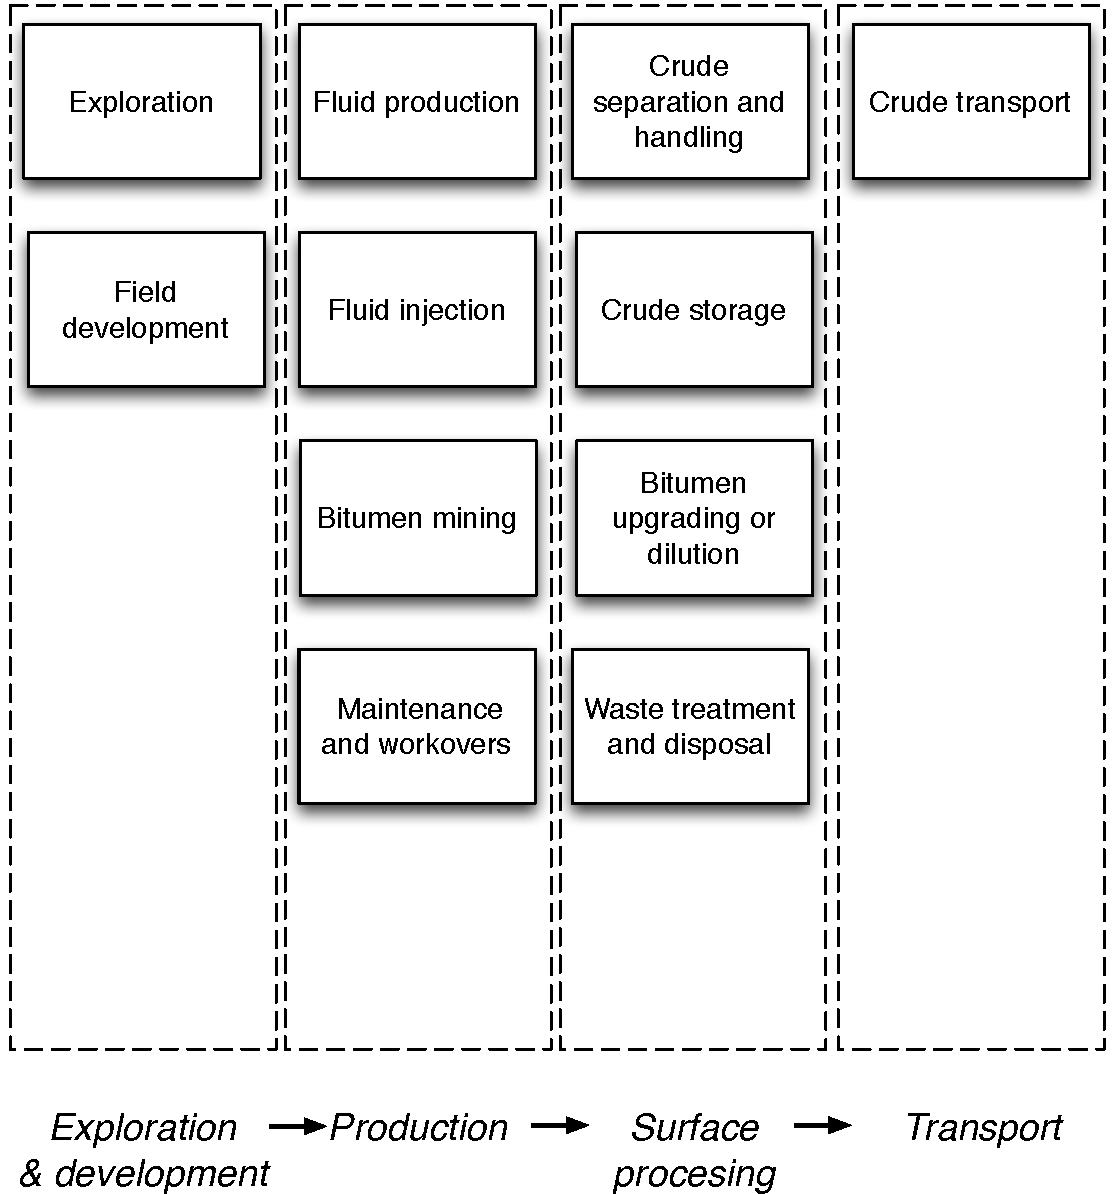
\includegraphics[width=0.85\columnwidth]{images/Flow_sheet_v4.pdf}
\caption{Schematic chart showing included stages within OPGEE for crude oil production.}
\label{fig:OPGEE_stages}
\end{figure}


\subsection{Spreadsheet structure}

OPGEE is modular in structure, with interlinked worksheets each representing a production or processing unit (sometimes called a ``unit process''). Streams connect each unit process with mass flows of oil, water, or numerous of gas species. Each unit process performs calculations representing the function of that process, resulting in output streams and an estimation of the energy use and emissions within that process. For example, the \sheet{Separation} sheet performs the calculations required to estimate the separation of the mixed oil, water, and gas stream from the wellbore into specific streams, and estimates the energy and emissions associated with that separation.

A number of summary sheets unite these process unit sheets, and provide overall summary results and naviagtion capabilities. These will be described in more detail below.

\subsection{Modeling detail and default specifications}

OPGEE models oil or natural gas production emissions in more detail than previous LCA models. For example, the energy consumed in lifting produced fluids (oil, water, and associated gas) to the surface is computed using the fundamental physics of fluid lifting, accounting for friction and pump efficiencies. 

Increased modeling detail results in an increase in the number of model parameters. All required inputs to OPGEE are assigned default values that can be kept as is or changed to match the characteristics of a given oil and/or gas field or marketable crude oil blend. If only a limited amount of information is available for a given facility, most input values will remain equal to defaults. In contrast, if detailed field-level data are available, a more accurate emissions estimate can be generated.

For some processes and sub-processes, correlations or relationships are developed for defaults, which we call ``smart defaults''. For example, the amount of water produced with oil (water-oil-ratio, or WOR) affects the energy consumed in lifting, handling, and separating fluids. If the WOR is known, it can be input directly into the model. However, in some regions, water production is not reported, so OPGEE includes a statistical relationship for water production as a function of reservoir age (see Section \ref{WORSmartDefault} for a description of the analysis underlying this smart default).

A workflow for updating and improving the data basis and accuracy of an emissions estimate using OPGEE is shown in Figure \ref{fig:OPGEE_flow}. This workflow represents one possible way that OPGEE could be used.


\begin{figure}[t]
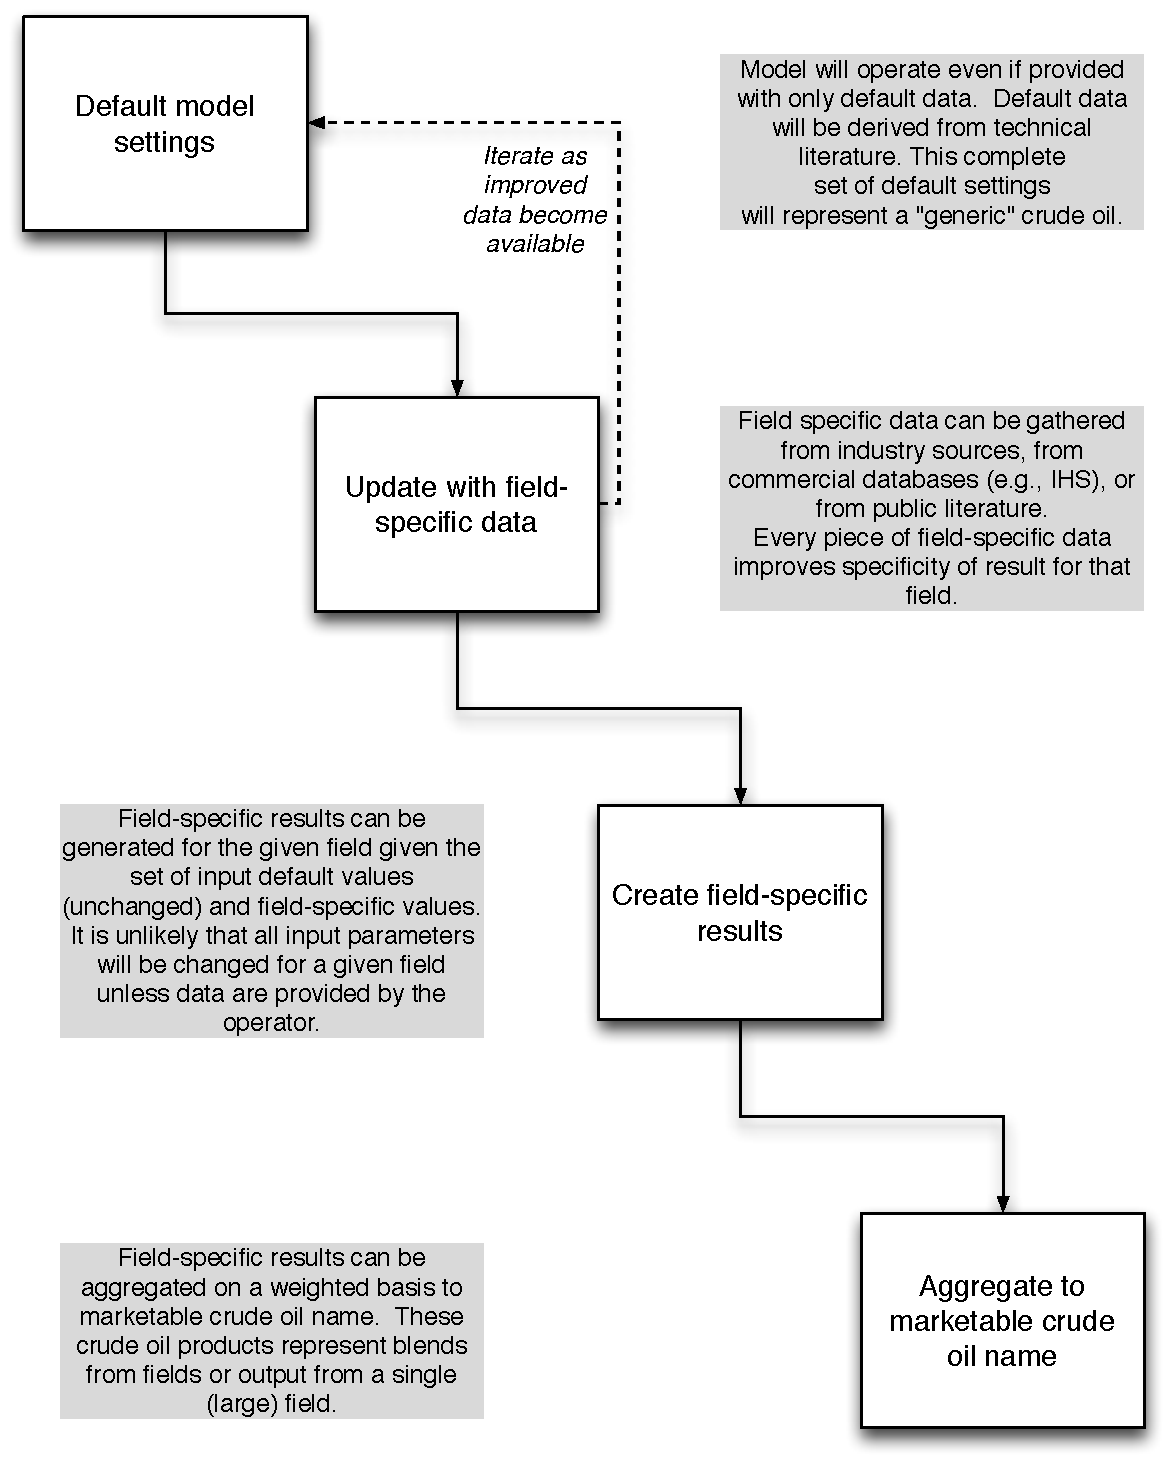
\includegraphics[width=0.8\columnwidth]{images/Flow_chart.pdf}
\caption{Proposed workflow for improving emissions estimates using OPGEE.}
\label{fig:OPGEE_flow}
\end{figure}




\subsection{Emissions sources classification}

Each process stage or sub-process in OPGEE can result in a variety of emissions sources. For example, the \sheet{Drilling \& Development} process stage includes the terrestrial drilling sub-process. Terrestrial drilling could include the following emissions sources:
\begin{itemize}
\item Combustion emissions from drilling rig prime mover;
\item Flaring emissions from drilling rig;
\item Vents and other upset emissions from drilling rig;
\item Combustion emissions from work performed in land clearing and site preparation;
\item Biogenic emissions from ecosystem disturbance during development;
\item Embodied emissions in cement and casing;
\item Embodied emissions in other consumable materials (e.g., fracturing sand)
\end{itemize}
Note that these emissions sources are of significantly different magnitude and have different causation and potential methods of mitigation. In total, over 100 emissions sources are classified in OPGEE \version across all process stages (e.g., all included processes and sub-processes). See Appendix \ref{sec:app_sources_classification} for a complete tabulation and classification of emissions sources.  Model coverage is also shown in the \sheet{Model Coverage} tab of OPGEE \version.



\subsection{Emissions source significance cutoffs}

It would be infeasible (and counter-productive) to attempt to estimate the magnitude of every emissions source listed in Appendix \ref{sec:app_sources_classification}. Fortunately, a small number of emissions sources will result in most of the emissions from petroleum production operations. 

For this reason, emissions sources included in the OPGEE system boundary are classified by estimated emissions magnitude. These emissions magnitudes are meant to represent \emph{possible} emissions magnitudes from a source, not the actual emissions that would result from that source for any particular field. An order-of-magnitude estimation approach is used, with each source assigned a rating in ``stars'' from one-star (*) to four-star (****) corresponding to 0.01 to 10 g CO$_2$ eq\ per MJ of crude oil delivered to the refinery gate. These classifications are explained in Table \ref{tab:emissions_significance}.

Emissions estimated to be one-star emissions (*) are not modeled in OPGEE due to insignificant magnitude. Since these small sources are known to have non-zero emissions, they are included in the overall emissions estimate by including a ``small sources'' term.  Two-star (**) sources are included simply or are included in the small sources term. Often, two-star sources are minor in magnitude, but are modeled due to the need to model the physics and chemistry of crude oil production and processing.\footnote{No strict criteria exist to determine the inclusion or exclusion of two-star sources. Modeler judgement is applied to determine the need for modeling these sources.} Three-star (***) sources are explicitly modeled in OPGEE. Four-star sources (****) are modeled in detail with stand-alone modules to allow variation, customization, and uncertainty analysis. 

\begin{table}
\begin{scriptsize}
\caption{Emissions classification, order of magnitude emissions, and significance description.}
\label{tab:emissions_significance}
\begin{tabular}{p{0.07\columnwidth}p{0.12\columnwidth}p{0.74\columnwidth}}
\toprule
Class & Est. mag. [gCO$_2$eq/MJ] & Description \\
\midrule
* & 0.01 & Minor emissions sources not worthy of further study or estimation. This is the most common classification. One-star emissions are accounted for by adding a value for miscellaneous minor emissions.\\
** & 0.1 & Minor emissions sources that are often neglected but may be included for physical completeness.\\
*** & 1 & Sources that can have material impacts on the final GHG estimate, and therefore are explicitly modeled in OPGEE. \\
**** & 10 & Sources that are large in magnitude (though uncommon). Examples include steam production for thermal oil recovery and associated gas flaring. These sources are significant enough to require their own dedicated OPGEE modules.\\
\bottomrule 
\end{tabular}
\end{scriptsize}
\end{table}


\subsection{Data sources}

Because of the need for transparent data basis, OPGEE uses data from a variety of technical reference works. For example, emissions factors are derived from standard engineering references from the American Petroleum Institute (API) and Environmental Protection Agency (EPA) \cite{EPA1995a, Shires2004}. A large number of technical references, journal articles, and fundamental data sources have been consulted during the construction of OPGEE, including: 
\begin{itemize}
\item Exploration and drilling \cite{Shires2004, Azar2007, Devereux1998, Gidley1989, Lapeyrouse2002, Mitchell2006, Mitchell2011, Wilson1999}
\item Production and surface separations \cite{Shires2004,  API1991, API1993a, API1995a, API1996b, API1998a, API2003, API2006, API2008a, API2008b, API2009a, API2009b, API2009c, API2009d, Arnold2007, Chilingarian1987, Chilingarian1989, Cholet2000, Clegg2007, Fanchi2007, GPSA2004, Holstein2007a, Holstein2007b, Leffler2006, Manning1991, Manning1995, Stewart2008, Stewart2009, Stewart2011, Takacs1993, Takacs2003}
\item Secondary and tertiary recovery \cite{Craig1993, Jarrell2002, Prats1985, Rose1989, Warner2007, Green1998}
\item Water treatment and waste disposal \cite{Wilson1999, Manning1995, Stewart2011, Khatib2002, Neff2007, Reed1996, Veil2004}
\item Venting, flaring, and fugitive emissions \cite{API1991, API1993a, API1995a, API1996b, API1998a, API1998b, API1998c, API2003, API2006, API2008a, API2008b, API2008c, API2009a, API1993b, API1995a, API2009e}
\item Petroleum transport and storage \cite{API2006, GPSA2004, API1993b, API1995b, API1997, API2009a, Mcallister2009, Miesner2006, Szilas1985}
\end{itemize}

%%%%%%%%%%%%%%%%%%%%%%%%%%%%%%%%%%%%%%%%%%%%%%%%
\clearpage

%%%%%%%%%%%%%%%%%%%%%%%%%%%%%%%%%%%%%%%%%%%%%
%%%%%%%%%%%%%%%%%%%%%%%%%%%%%%%%%%%%%%%%%%%%%
%%%%%%%%%%%%%%%%%%%%%%%%%%%%%%%%%%%%%%%%%%%%%

%\chapter{User Guide}
%
%\section{OPGEE Quick Start Guide}
%
%This section explains the basics of how to work with OPGEE. We divide OPGEE interactions into two separate use categories: (i) basic OPGEE interaction, and (ii) advanced OPGEE interaction. Brief guidance is provided for each use case, with frequent reference to more detailed explanations of OPGEE components in the technical documentation sections. See the next section, Section \ref{sec:guided_example}, for a guided example, and the OPGEE sheets referenced here are also described in more detail in the User Guide, in section \ref{sec:model_structure}.
%For the purposes of explanation, we divide OPGEE use into three key steps:
%
%
%\begin{itemize}
%\item Model formulation: The user establishes the goal and scope of the analysis. This involves specifying the LCA parameters of interest such as the reference unit of energy (e.g., functional unit), product system of interest (e.g., boundary), and how co-production accounting is handled.
%\item Parameter input: The user inputs data for an oil and gas field or multiple fields. Multiple types of data inputs exist, but the most important ones exist on the \sheet{Inputs} worksheet.
%\item Results viewing: OPGEE has multiple results viewing sheets which communicate key information related to emissions intensity, fugitives and venting, uncertainty, and model errors.
%\end{itemize}
%%%%%%%%%%%%%%%%%%%%%%%%%%%%%%%%%%%%%%
%\subsection{Basic OPGEE interaction} 
%
%At the simplest level, the easiest way to use OPGEE is to investigate GHG emissions for a single oil field. OPGEE analysis of a single field only requires the user to navigate two sheets, the \sheet{Inputs} worksheet and the \sheet{Active Field} worksheet. 
%
%%For an overview of the three key steps applied to basic OPGEE interaction, see Figure \ref{fig:basic_flow}.
%
%\clearpage
%
%%\begin{figure}[t]
%%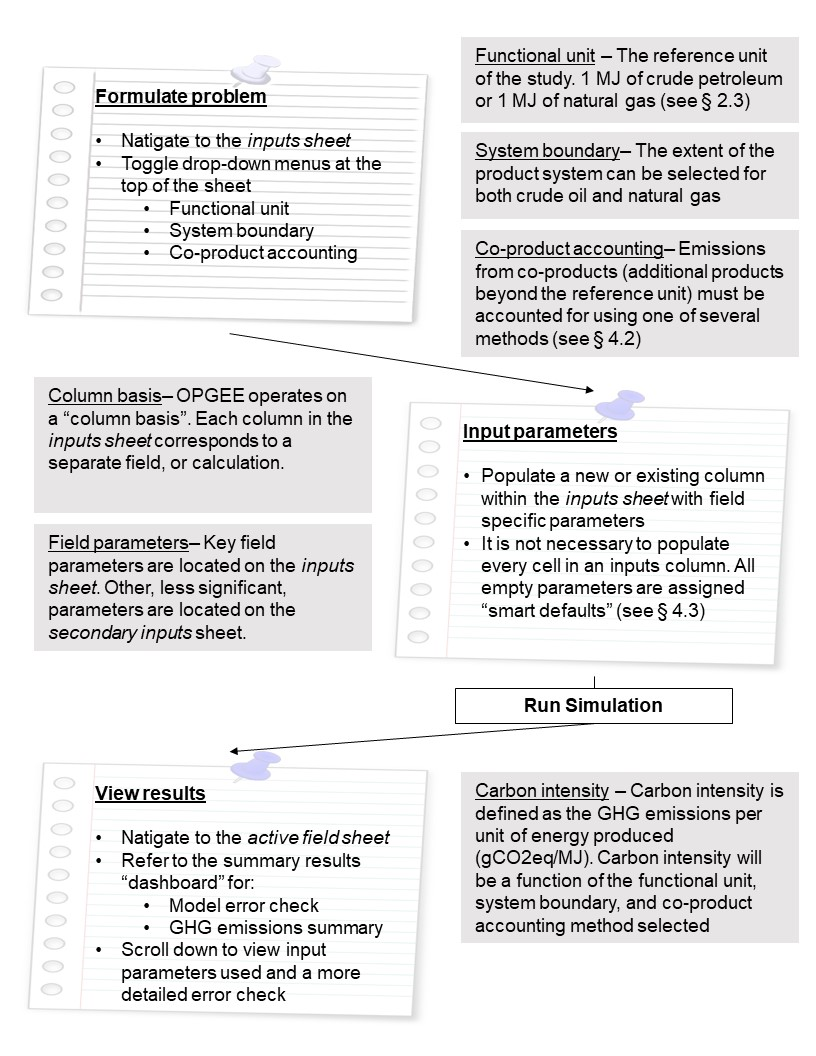
\includegraphics[width=1\columnwidth]{documentation/images/User_Guide_figs/basic.jpg}
%%\caption{Quick-start flowchart for basic operation}
%%\label{fig:basic_flow}
%%\end{figure}
%%
%%\clearpage
%
%%%%%%%%%%%%%%%%%%%%%%%%%%%%%%%%%%%%%%
%\subsection{Advanced OPGEE interaction} 
%
%Most OPGEE usage requires analysis beyond one realization of a single oil field. Advanced OPGEE interactions include:
%
%\begin{itemize}
%\item Simulating more than one field in a single OPGEE instance. This is a useful feature that saves time by ``batching'' fields to run at once versus simulating each one individually.
%\item Simulating multiple realizations in order to conduct a Monte Carlo uncertainty analysis. Due to issues with missing data, it is important to understand the uncertainty of your GHG emissions estimate.
%\end{itemize}
%
%Each of these analyses requires the user interact with OPGEE beyond the \sheet{Inputs} worksheet and the \sheet{Active Field} worksheet. These include the \sheet{Secondary Inputs}, \sheet{Results}, and \sheet{Uncertainty} worksheets. For an overview of the three steps (model formulation, parameter input, and results viewing) applied to these advanced OPGEE interactions, see Figure \ref{fig:multiple_flow}, Figure \ref{fig:gassy_flow}, and Figure \ref{fig:uncertainty_flow}.
%
%%\clearpage
%%
%%\begin{figure}[t]
%%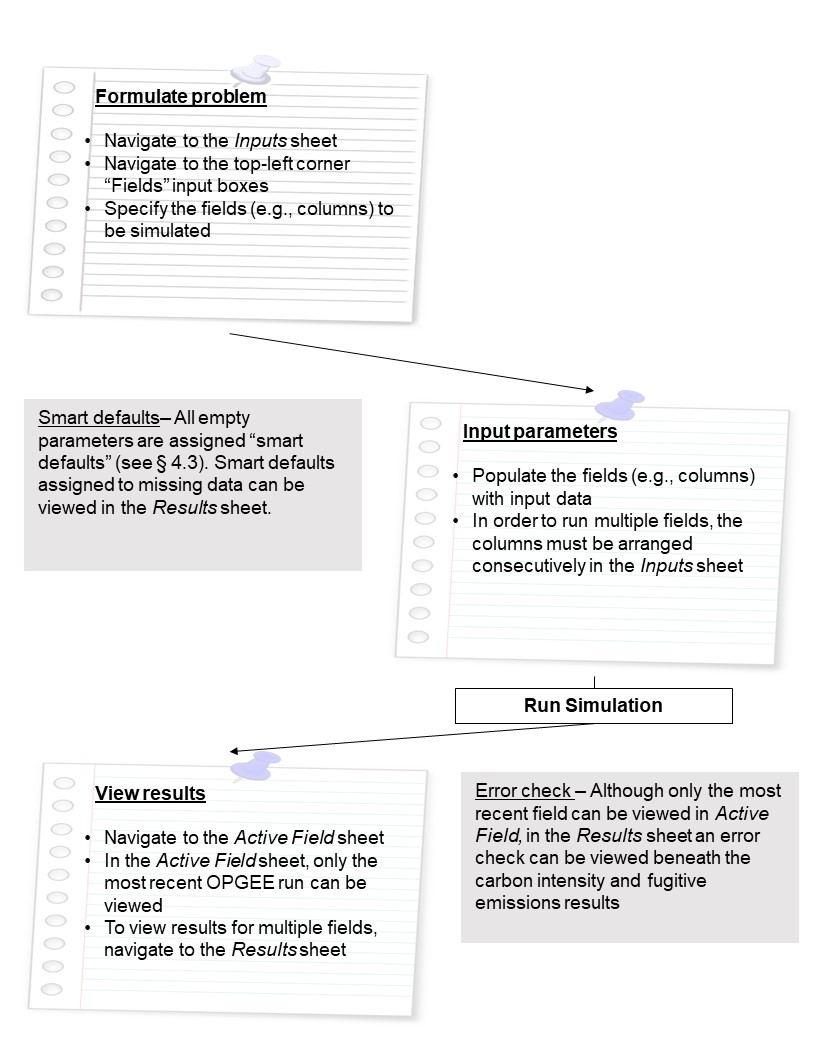
\includegraphics[width=1\columnwidth]{documentation/images/User_Guide_figs/multiple.jpg}
%%\caption{Quick-start flowchart for running multiple fields}
%%\label{fig:multiple_flow}
%%\end{figure}
%%
%%\clearpage
%%
%%\begin{figure}[t]
%%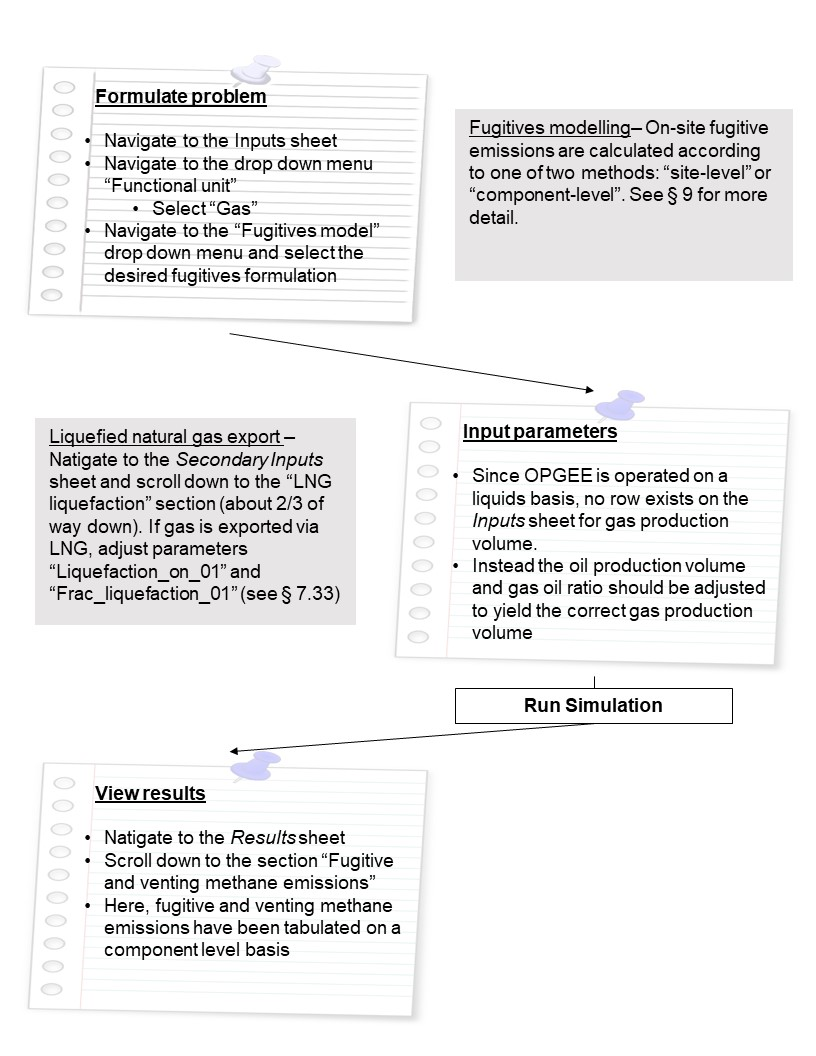
\includegraphics[width=1\columnwidth]{documentation/images/User_Guide_figs/gassy.jpg}
%%\caption{Quick-start flowchart for running gas-rich fields}
%%\label{fig:gassy_flow}
%%\end{figure}
%%
%%\clearpage
%%
%%\begin{figure}[t]
%%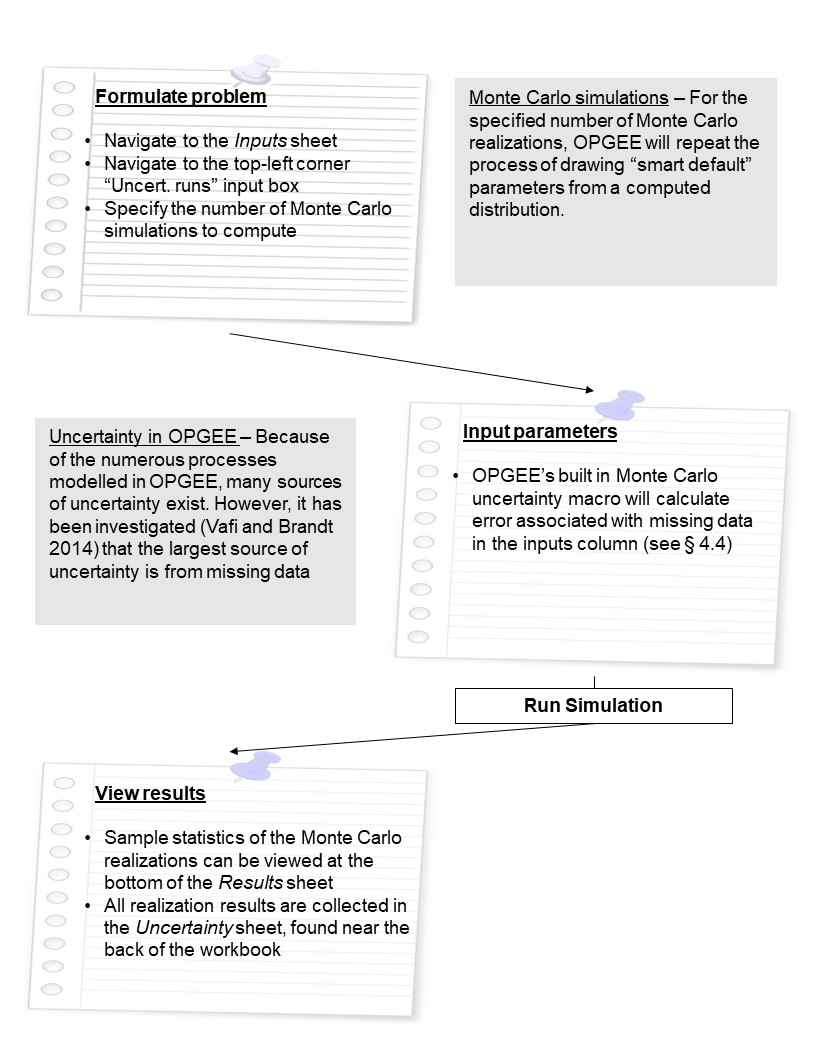
\includegraphics[width=1\columnwidth]{documentation/images/User_Guide_figs/uncertainty.jpg}
%%\caption{Quick-start flowchart for running fields with uncertainty analysis}
%%\label{fig:uncertainty_flow}
%%\end{figure}
%
%\clearpage
%
%\section{Example OPGEE calculation} \label{sec:guided_example}
%
%In order to demonstrate the steps described in previous sections of the User Guide, this section will provide a step-by-step OPGEE example applied to three different crude oils. In the first part, we look simply at basic OPGEE operation. In the second part, we will look at uncertainty analysis of the same three crude oils.
%For illustration of how key parameters affect crude oil GHG intensity, we have selected three distinctive field types (Table \ref{tab:example_parameters}). These field types, gas-rich, heavy, and tight, are based on approximate data from US fields Prudhoe Bay (Alaska), Midway Sunset, (California) and Eagle Ford (Texas), respectively.
%
%\begin{table}[ht]
%\begin{scriptsize}
%\caption{Key parameter inputs for example oil fields}
%\label{tab:example_parameters}
%\begin{tabular*}{1\columnwidth}{p{0.2\columnwidth}p{0.2\columnwidth}p{0.2\columnwidth}p{0.3\columnwidth}}
%\toprule
%Parameter & Gas-rich & Heavy & Tight \\
%\midrule
%Production methods & Water flooding, Gas reinjection/lifting & Steam flooding & Hydraulic fracturing/ horizontal drilling \\
%Field age [yrs] & 27 & 115 & 6 \\
%Oil production rate [bbls/day] & 354473 & 93407 & 462000 \\
%Gas-oil ratio [scf/bbl] & 22615 & 93 & 906 \\
%No. production wells & 700 & 11392 & 3695 \\
%API gravity [degAPI] & 29 & 19 & 46 \\
%\bottomrule
%\end{tabular*}
%\end{scriptsize}
%\end{table}
%
%\subsection{Basic OPGEE interaction} 
%
%\subsubsection{Model formulation}
%
%The following need to be considered in formulating an OPGEE run:
%
%\begin{itemize}
%\item Functional unit: Because these fields are primarily oil producers, we select the functional unit to be 1 MJ of crude petroleum.
%\item System boundary: For this analysis, we wish to include emissions including transportation of the key product (oil) to the refinery gate, so we select 'oil boundary' to be 'Refinery'.
%\item Co-product accounting: The method of co-product accounting should be chosen considering the methodologies of other studies the results might be compared to. These results won't be used for any comparisons, so we use the allocation methodology. In the allocation methodology, emissions are divided proportionally between products and co-products according to energy output. The alternative, co-product displacement, applies emissions credits/debits according to the average emission intensity of products that would be displaced in the economy by the production of the co-product.
%\item Fugitives modelling: A variety of related approaches are applied in OPGEE to estimate venting and fugitive emissions. For this example, we select the 'site-level approach'. More detail on these approaches is provided in Section \ref{sec:VFF}.
%\end{itemize}
%
%See Figure \ref{fig:lca_specs} below for the locations of adjustable model parameters on the \sheet{Inputs} worksheet.
%
%\begin{figure}
%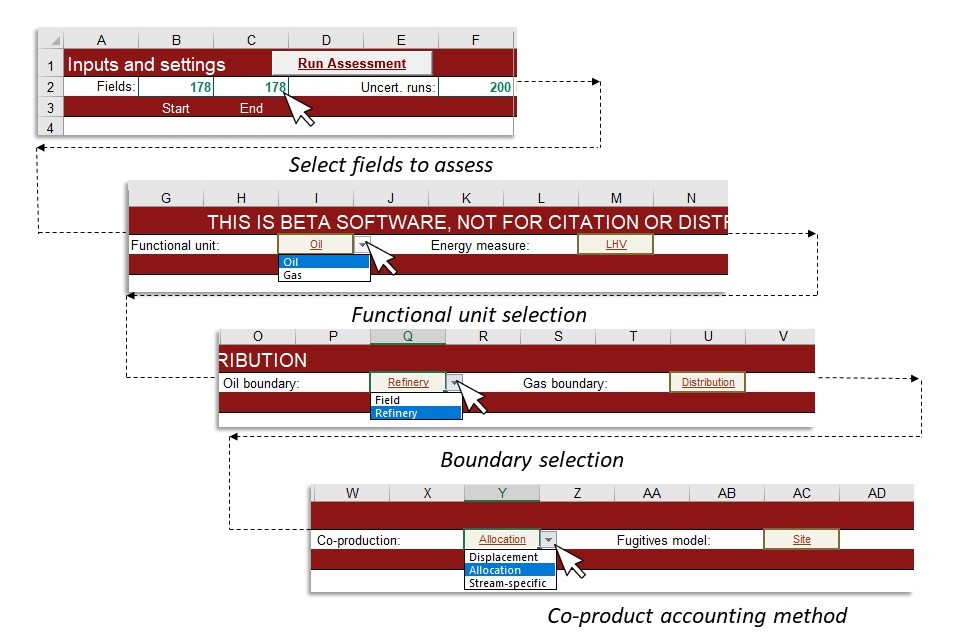
\includegraphics[width=1\columnwidth]{documentation/images/User_Guide_figs/lcaspecs_2.jpg}
%\caption{Screenshot demonstrating locations of OPGEE model parameters on the \sheet{Inputs} worksheet}
%\label{fig:lca_specs}
%\end{figure}
%
%\subsubsection{Input parameters}
%
%We populate columns 1-3 with data collected for our three oil fields. A single column in OPGEE is parameterized according to operating conditions for a single year. Therefore, the resulting CI provides a static estimate of emissions for a barrel of oil from a single oil field at a specific point in time. For those parameters that lack data, we leave the cells blank. In the absence of data inputs, OPGEE generates ``smart defaults'': statistically determined parameters designed to be representative of known oil and gas fields (with distributions generated from a global dataset, for more on smart defaults see Section \ref{sec:smart_defaults}). 
%
%For basic interaction, we will run each field one at a time with one uncertainty realization (recalling that the \sheet{Active Field} sheet only displays information one field at a time). In the case of our tight oil field, we note that horizontal drilling and hydraulic fracturing need to be turned on in the \sheet{Secondary Inputs} worksheet (as a first approximation, navigate to ``Drilling \& development'' in \sheet{Secondary Inputs} and set ``Fraction of wells fractured'' and ``Horizontal well?'' to ``1'').
%
%\begin{figure}[ht]
%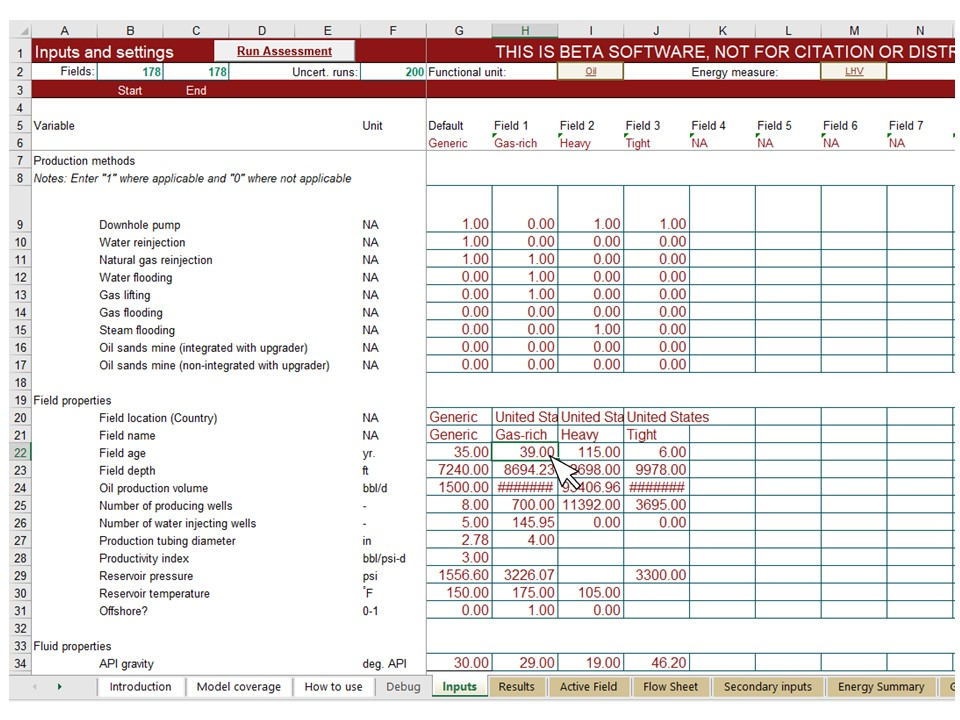
\includegraphics[width=1\columnwidth]{documentation/images/User_Guide_figs/inputs.jpg}
%\caption{Screenshot of input data entered into the \sheet{Inputs} worksheet}
%\label{fig:example_inputs}
%\end{figure}
%
%\subsubsection{Results viewing}
%
%The \sheet{Active Field} worksheet is the primary hub for gathering information relevant to the most recent model run. Here, model inputs for missing data are generated, results are gathered from \sheet{GHG Summary} and \sheet{Energy Summary}, and a detailed error check is done.
%
%Also on the \sheet{Active Field} sheet, key information is summarized in the summary results dashboard. 
%
%\begin{itemize}
%\item Error checking: If any errors are identified here, the source can be found at the bottom of the active field worksheet.
%\item Co-product balance: It is important to check if high shares of secondary product imports/exports are driving emissions. This is often the cased for mixed gas/oil fields.
%\end{itemize}
%
%\begin{figure}[!htbp]
%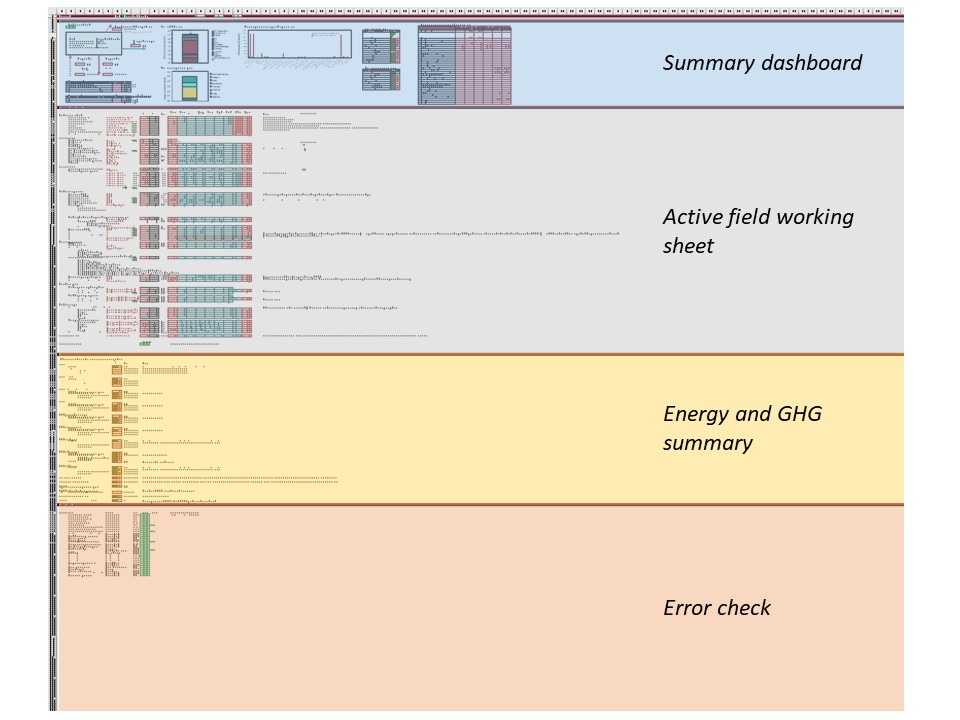
\includegraphics[width=1\columnwidth]{documentation/images/User_Guide_figs/activefield.jpg}
%\caption{\sheet{Active Field} worksheet at maximum zoom with major regions color coded and labelled}
%\label{fig:example_activefield}
%\end{figure}
%
%After checking that our results are error-free, we look at emissions results. Figure \ref{fig:example_ghgsummary} contains GHG emissions results for our three fields, each copied directly from the \sheet{Active Field} sheet. From these plots we can gather the total carbon intensity of each field, as well as the process-level breakdown of emissions. Clearly, the most intensive field is Midway Sunset, due to processing related emissions (looking closer in the \sheet{Energy Summary} sheet, it can be determined that these processing emissions are associated with treatment of produced water). Figure \ref{fig:example_vffsummary} contains source-specific venting and fugitive emissions for our three fields, also copied directly from the \sheet{Active Field} sheet. From this plot we gather that the gassiest field (Prudhoe Bay) has the most intensive venting and fugitive emissions, while the least gassy field (Midway Sunset) has the least intensive venting and fugitive emissions. For Prudhoe Bay, venting and fugitive emissions are largely explained by leaks during extraction (e.g., wellhead and separator) and transportation of the gas (e.g., gathering, transmission, and distribution).
%
%\begin{figure}[!htbp]
%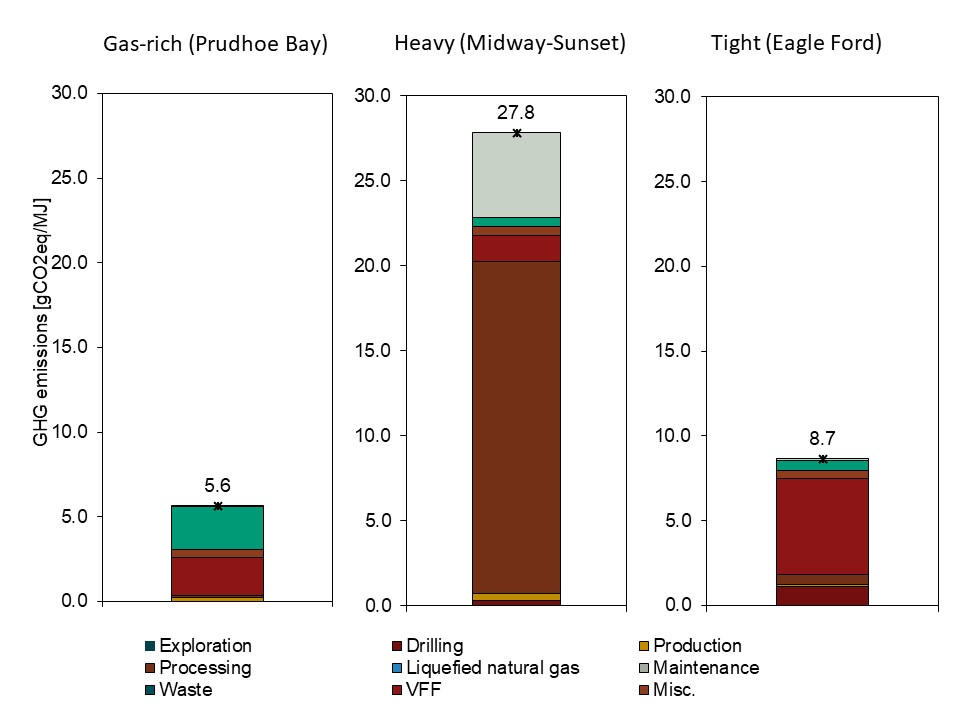
\includegraphics[width=1\columnwidth]{documentation/images/User_Guide_figs/ghgintensity.jpg}
%\caption{Summary GHG emissions results for three example fields, broken down by process stage}
%\label{fig:example_ghgsummary}
%\end{figure}
%
%% issue 1: are you sure the y-axis unit is correct? 
%
%\begin{figure}[!htbp]
%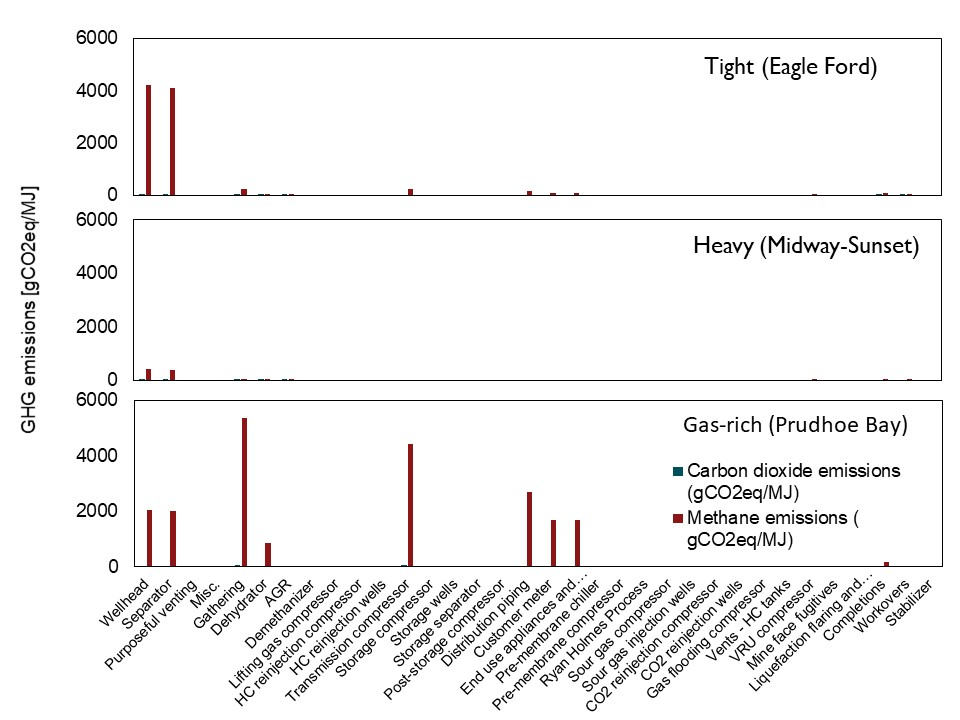
\includegraphics[width=1\columnwidth]{documentation/images/User_Guide_figs/vffsource.jpg}
%\caption{Summary venting and fugitive emissions for summary fields, broken down by source}
%\label{fig:example_vffsummary}
%\end{figure}
%
%\clearpage
%
%\subsection{Uncertainty analysis} 
%
%For this analysis, we wish to assess error for 200 Monte Carle realizations. Inputs for multiple fields can be handled sequentially in a single OPGEE ``run'' from the \sheet{Inputs} worksheet. Again recalling that hydraulic fracturing and horizontal drilling need to be adjusted in \sheet{Secondary Inputs} for our tight oil field, we split our model runs into two batches. One run includes 200 realizations each of our gassy and heavy fields, and our second run includes 200 realizations of our tight oil field (with adjustments in \sheet{Secondary Inputs}).
%After running the model, we perform analysis using the 200 realizations gathered in the \sheet{Uncertainty} worksheet. For this analysis, plotting is not performed in OPGEE, so we post-process the data in Matlab. For each field, a GHG intensity value was iteratively pulled from the OPGEE generated data as a new realization, and added to the pool of realizations. At each iteration, the sample mean ($\bar{\mu_{CI}}$) and standard deviation ($\bar{\sigma_{CI}}$) of the pool is recorded. In this way, we test the effect of number of realizations on $\bar{\mu_{CI}}$ and $\bar{\sigma_{CI}}$. By comparing how our three different fields behave, we can assess how data availability affects the number of realizations required for stable values of $\bar{\mu_{CI}}$ and $\bar{\sigma_{CI}}$. Based on our results (Figure \ref{fig:example_uncertainty_1}), $\bar{\mu_{CI}}$ stabilizes very quickly, and $\bar{\sigma_{CI}}$ stabilizes at a small value (less than 1 gCO$_2$eq/MJ for all fields) after about 100 realizations.
%
%\begin{figure}[ht]
%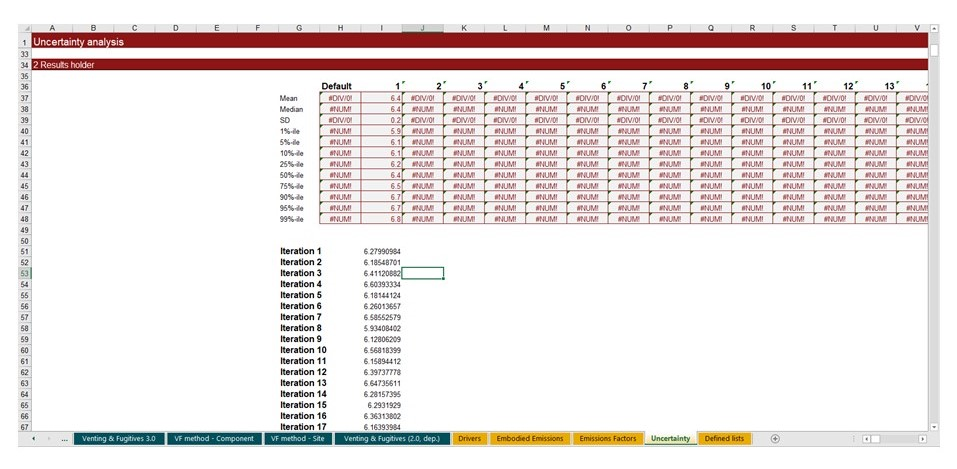
\includegraphics[width=1\columnwidth]{documentation/images/User_Guide_figs/uncertaintypage_2.jpg}
%\caption{Screenshot of \sheet{Uncertainty} worksheet}
%\label{fig:uncertaintypage}
%\end{figure}
%
%\begin{figure}[!htbp]
%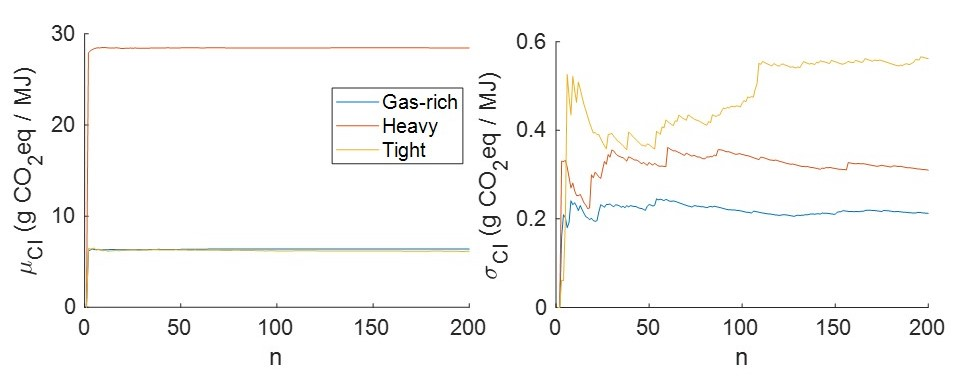
\includegraphics[width=1\columnwidth]{documentation/images/User_Guide_figs/uncertaintyresults_2.jpg}
%\caption{$\bar{\mu_{CI}}$ and $\bar{\sigma_{CI}}$ versus number of Monte Carlo realizations (n).}
%\label{fig:example_uncertainty_1}
%\end{figure}
%
%% issue 2: Jeff: move all three plots of figure 3.12 in one column
%
%\begin{figure}[!htbp]
%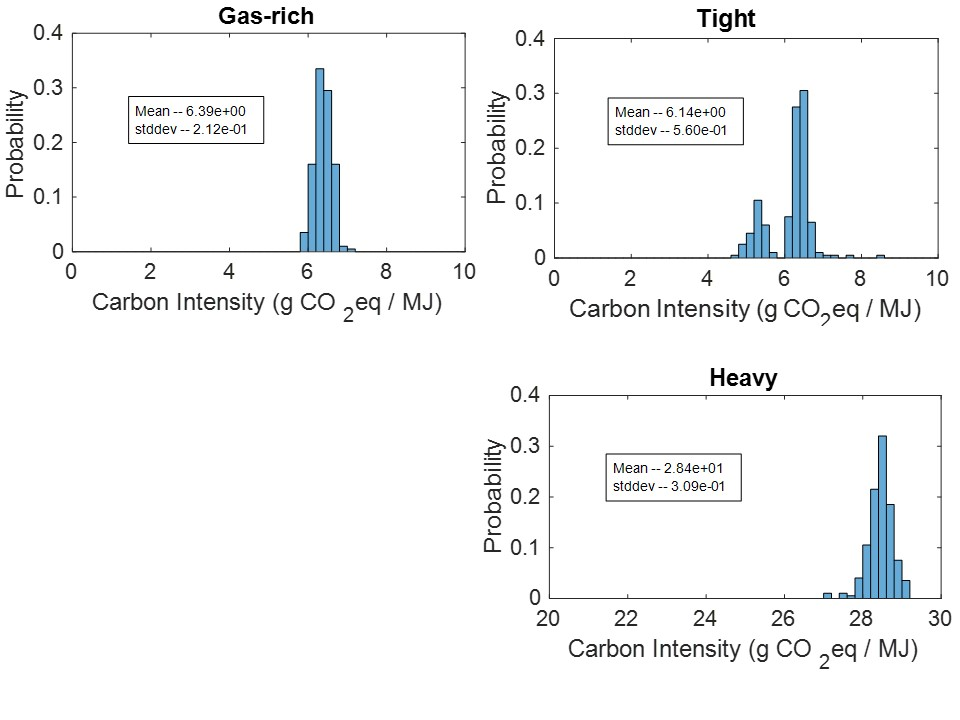
\includegraphics[width=1\columnwidth]{documentation/images/User_Guide_figs/histos.jpg}
%\caption{Histogarms of GHG intensity (CO$_2$eq/MJ) over 200 Monte Carlo simulations.}
%\label{fig:example_uncertainty_2}
%\end{figure}
%
%\clearpage

%%%%%%%%%%%%%%%%%%%%%%%%%%%%%%%%%%%%%
\section{OPGEE model structure}
\label{sec:model_structure}

OPGEE is composed of numerous worksheets, each of which can be categorized into one of five types: (1) input sheets, (2) field summary sheets, (3) process stage worksheets, (4) supplementary worksheets, and (5) output gathering worksheets. The excel tabs are colored beige, green, red, yellow, and grey, respectively. Navigating OPGEE worksheets is much easier if one has an understanding of how these five worksheet types interact (Figure \ref{fig:model_structure}). In this section, we will briefly describe each type of OPGEE worksheet.

\begin{landscape}
\begin{figure}[ht]
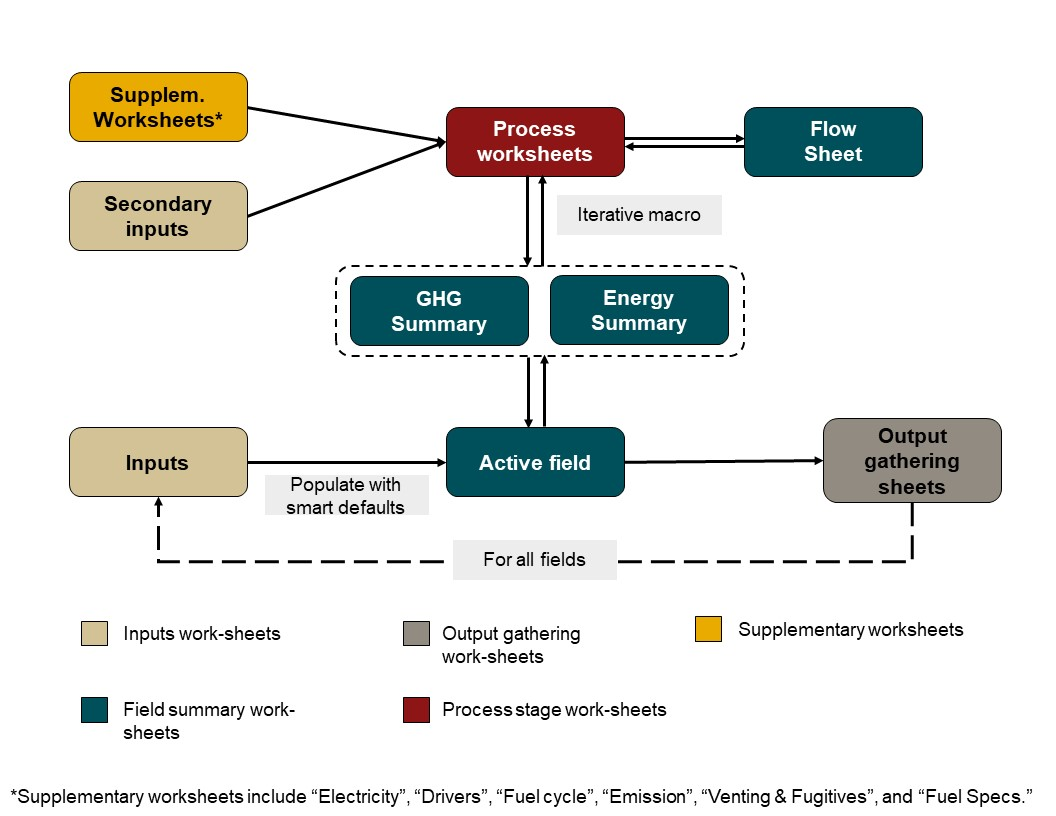
\includegraphics[width=1\columnwidth]{images/Fig_3.jpg}
\caption{OPGEE model workflow according to worksheet types).}
\label{fig:model_structure}
\end{figure}
\end{landscape}

In using the OPGEE workbook, the user will encounter different types of cells. Some cells are free to adjust (mostly input sheets) and some aren't (mostly process and supplementary worksheets). As shown in Figure \ref{fig:cell_types} below, User Free and Default Free cells are included with light tones, while User Locked and Default Locked cells are included with dark tones. In general, the user is advised to not change cells with dark background colors.

\begin{figure}[ht]
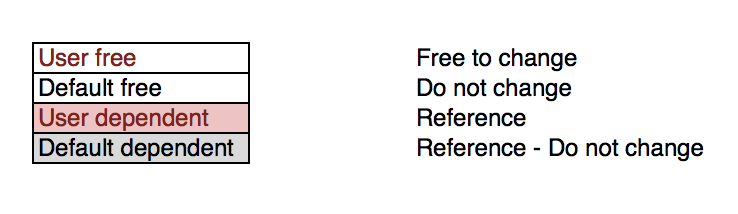
\includegraphics[width=1\columnwidth]{images/Cell_Types.png}
\caption{Types of cells. User Free and Default Free cells can be changed, while Locked cells should not be changed due to possibility of compromising model functionality. Flow sheet cells are either calculated in place or looked up from the large flow table.}
\label{fig:cell_types}
\end{figure}

\subsection{Input worksheets} 

OPGEE input data is classified as either ``primary input data'' or ``secondary input data''. Primary and secondary input data are divided between the \sheet{Inputs} worksheet and the \sheet{Secondary Inputs} worksheet.

\subsubsection{\sheet{Inputs} worksheet}

Primary input data are entered on the \sheet{Inputs} worksheet. This worksheet is labeled `Inputs' and is colored beige. Primary input data includes those parameters most important to calculation of carbon intensity. Primary input data share several common characteristics: (i) They have a significant effect on the GHG emissions from an oil and gas operation, (ii) they vary significantly across different operations and therefore could cause variability between different fields or projects, and (iii) they are likely to be measured or are well-understood by operators. Primary input data for hundreds of fields can be entered on the \sheet{Inputs} sheet. The data entered by the user are stored without modification, so the \sheet{Inputs} worksheet can be used to compile and store data for a variety of operations.

OPGEE v3.0a is run from the inputs worksheet. The user enters the starting field of analysis and the ending field of analysis and presses the ``Run Assessment'' button.

\subsubsection{\sheet{Secondary Inputs} worksheet} 

Secondary input data are entered on the \sheet{Secondary Inputs} worksheet. All secondary input parameters are free for the user to change, however, it should not be necessary to change these secondary input parameters in basic use of OPGEE. The secondary parameters include parameters with less effect on the resulting emissions, that are not highly variable across operations, or that are less likely to be known by model users. Examples include compressor suction pressure and temperature, type of prime mover, or pump efficiency. Note that some of these parameters (e.g., pump efficiency) can have significant effects on model results, but are not believed to be highly variable across fields.

\subsection{Field summary worksheets} 

Field summary worksheets present information about the field most recently analyzed. Field summary worksheets are colored dark green. The overall summary inputs and results for the field under analysis are presented on the \sheet{Active Field} sheet. Flows for the field under analysis are presented and organized in the \sheet{Flow Sheet} worksheet. Process stage calculations are compiled into summed energy consumption results (including energy co-production credits) on the \sheet{Energy Summary} sheet and summed GHG emissions (including any offsets from co-produced energy) on the \sheet{GHG Summary} sheet. Lastly, a summary of venting and fugitive emissions are presented in the \sheet{VFF Summary} worksheet.

\subsubsection{\sheet{Active field} worksheet}

The \sheet{Active field} worksheet presents summary inputs and results in tabular and graphical form for the most recently processed field. After a run involving multiple fields, \sheet{Active field} retains the data from last field assessed and does not save results for prior fields. \sheet{Active field} allows for detailed tracking and analysis of the results for an individual field. If one wants to debug results or explore results further for a particular field, it is recommended that they enter just that field number on the input sheet and then explore working backward from the \sheet{Active field} worksheet.

The \sheet{Active field} worksheet serves as a holding place for information on the field currently under analysis during a particular OPGEE run, and logic on the sheet applies many of the ``smart defaults'' defined below. For this reason, the \sheet{Active field} worksheet should not be modified by the user (at least without great care).

\subsubsection{\sheet{Flow Sheet} worksheet} 

The \sheet{Flow Sheet} worksheet tracks all flows into and out of each process unit for the active field. All flows for a set of tracked liquid, gas, and solid products are tracked from primary extraction from geologic deposits until final disposition. The flow sheet is also the key sheet for navigating to process level calculations via the process flow diagram presented below the large table of flows.

\subsubsection{\sheet{Energy Summary} worksheet}

The \sheet{Energy Summary} worksheet gathers data on energy consumption for sub-processes from all process worksheets. Each main process worksheet is included in the gathering table. All energy consumed is summed by type across all stages. This gross consumption is used to compute net consumption and energy imports and exports. The energy consumption worksheet is described in Section \ref{sec:energy_consumption}.

\subsubsection{\sheet{GHG Summary} worksheet} 

The \sheet{GHG Summary} worksheet gathers and summarizes the emissions computed in each process worksheet. Emissions are computed as tonne CO$_2$eq/d. The \sheet{GHG Summary} worksheet is described in Section \ref{sec:GHG_emissions}.

\subsection{Process stage worksheets} 

Process stage worksheets form the core of OPGEE, and are where most model calculations occur. These worksheets have red-colored tabs.
Process stage worksheets are most easily accessed through the \sheet{Flow Sheet} worksheet, where each process unit or process stage is represented by a box with a ``go to'' button. Press the ``go to'' button for each process unit to jump to that process unit to examine calculations. 

Most process stage worksheets are divided into three main sections: (1) Flows, (2) Calculations, and (3) Outputs.

\begin{itemize}
\item The \emph{flows} section of each process stage worksheet tracks mass flows into the process and flows out of the process. Flows are denominated in tonnes per day (with the exception of electricity, denominated in MWh per day). 
Flow cells are bold if directly computed in that sheet, and standard weight font if drawn directly from the flow table (for example, as an input to the process unit.
\item Below the flows section is the \emph{calculations} section of a worksheet, where intermediate model outputs are calculated. These intermediate outputs are summarized and compiled by the gathering worksheets to provide the overall energy and emissions measures compiled in the \sheet{Active field} worksheet.
Note that process stage worksheets refer to the inputs worksheet and secondary inputs worksheet through the use of ``named ranges''. The named ranges are defined on the \sheet{Active field} worksheet (for primary inputs) and \sheet{Secondary Inputs} worksheet and make it easier for the user to understand formulas.
\item The outputs section holds the summary results in terms of energy use and emissions that are later collected in the summary sheets.
\end{itemize}

\subsection{Supplementary worksheets} 

Supplementary worksheets support calculations throughout OPGEE, including: calculating intermediate outputs in the process stage worksheets, compiling output in the gathering worksheets, and calculating results in the \sheet{Active field} worksheet. Supplementary worksheets have yellow-colored tabs.

\subsubsection{\sheet{Electricity} worksheet}

This worksheet includes the offsite electricity mix and calculates the energy consumption in onsite electricity generation (other than electricity co-generated with steam).

\subsubsection{\sheet{Drivers} worksheet} 

This worksheet provides a database of energy consumption for different types and sizes of prime movers (gas and diesel engines, gas turbines and electric motors). The \sheet{Drivers} worksheet is described in Section \ref{sec:drivers}.

\subsubsection{\sheet{Fuel cycle} worksheet}

This worksheet retrieves and calculates the fuel cycle energy consumption and GHG emissions for the calculation of credits/debits from fuel exports/imports. The \sheet{Fuel cycle} worksheet is described in Section \ref{sec:fuel_cycle}.

\subsubsection{\sheet{Emission factors} worksheet} 

This worksheet retrieves and builds emissions factors for the calculation of combustion and non-combustion GHG emissions from energy use and losses. The \sheet{Emission factors} worksheet is described in Section \ref{sec:emissions_factors}.

\subsubsection{\sheet{Venting \& Fugitives 3.0} worksheet} 

This worksheet calculates in detail the GHG emissions associated with venting and fugitives. The \sheet{Venting \& Fugitives 3.0} worksheet is described in Section \ref{sec:VFF}. Sub-worksheets that feed into the  \sheet{Venting \& Fugitives 3.0}  worksheet are \sheet{VF - Component}, \sheet{VF - Site - onsite}, \sheet{VF - Site - offsite}, and \sheet{VF - Secondary prod}. A copy of the deprecated OPGEE v2.0 fugitives assessment method is retained on the worksheet \sheet{Venting \& Fugitives (2.0, deprec.)}.

\subsubsection{\sheet{Fuel Specs} worksheet}

This worksheet provides fuel specifications required for OPGEE calculations. The \sheet{Fuel Specs} worksheet is described in Section \ref{sec:data_inputs}.

\subsubsection{\sheet{Constants} worksheet} 

This worksheet provides other needed data inputs such as conversion factors and steam enthalpies. 

\subsection{Output gathering worksheets} 

\subsubsection{\sheet{Results} worksheet}

After the user enters data to the \sheet{Inputs} worksheet and clicks the 'Run Assessment' button, OPGEE computes the resulting GHG emissions. The results for the last field (End field number entered on \sheet{Inputs} sheet) analyzed are stored in the \sheet{Active field} worksheet, while the results from all fields in the analyzed set are stored in the \sheet{Results} worksheet in tabular form in gCO$_2$ (equivalent GHG emissions per MJ LHV crude oil delivered to the refinery gate). Emissions are broken down by stage (generally) or by type, with venting, flaring, and fugitive emissions for all process stages summed together for convenient interpretation as `VFF' emissions. Total energy consumed per unit of energy delivered to the refinery gate is also presented in tabular and graphical form.

\subsubsection{\sheet{Uncertainty} worksheet} 

If the user conducts a Monte Carlo analysis (enters >1 uncertainty runs in the \sheet{Inputs} worksheet), the multiple realizations are collected in the \sheet{Uncertainty} worksheet. Sample statistics are also calculated here. Using the tabulated realizations, the user can conduct further uncertainty analysis in Matlab or Excel.

\clearpage

%%%%%%%%%%%%%%%%%%%%%%%%%%%%%%%%%%%%%

%%%%%%%%%%%%%%%%%%%%%%%%%%%%%%%%%%%%%%%%%%%%%
%%%%%%%%%%%%%%%%%%%%%%%%%%%%%%%%%%%%%%%%%%%%%
%%%%%%%%%%%%%%%%%%%%%%%%%%%%%%%%%%%%%%%%%%%%%

\part{Technical documentation}

%%%%%%%%%%%%%%%%%%%%%%%%%%%%%%%%%%%%%%%%%%%%%
%%%%%%%%%%%%%%%%%%%%%%%%%%%%%%%%%%%%%%%%%%%%%
%%%%%%%%%%%%%%%%%%%%%%%%%%%%%%%%%%%%%%%%%%%%%





%%%%%%%%%%%%%%%%%%%%%%%%%%%%%%%%%%%%%%%%%%%%%
%%%%%%%%%%%%%%%%%%%%%%%%%%%%%%%%%%%%%%%%%%%%%
%%%%%%%%%%%%%%%%%%%%%%%%%%%%%%%%%%%%%%%%%%%%%

\chapter{\sheet{Active Field} gathering worksheet}
\label{sec:active_field}


\clearpage

%%%%%%%%%%%%%%%%%%%%%%%%%%%%%%%%%%%%%
\section{Introduction to the \sheet{Active Field} worksheet}

The \sheet{Active field} worksheet presents a summary and holding place of information for the most recently analyzed field and realization (for example, if multiple fields 6-10 are analyzed, \sheet{Active field} will only retain information for the last model run -- field 10 -- and not for prior fields). At the top of the \sheet{Active field} worksheet is a summary dashboard of information related to co-product allocation and process-specific GHG intensity. Below the summary dashboard is a holding place of user specified and ``smart default'' generated input data. Next on the \sheet{Active field} worksheet is the energy and GHG summary. Lastly, a set of error checks are listed.

%%%%%%%%%%%%%%%%%%%%%%%%%%%%%%%%%%%%%
\section{Energy and GHG calculations on the \sheet{Active Field} worksheet}
Energy intensity and GHG emissions on the \sheet{Active Field} sheet are calculated by process stage (e.g., Production \& Extraction). 

For a given process stage $i$, the energy intensity in [MJ/MJ output] is computed. First the total energy consumption in stage $i$ is gathered from \sheet{Energy Summary} (see Eq. \ref{eq:energy_intensity}). This is then divided by the total energy output for purposes of constructing the denominator of the intensity ratio. This is also computed on the \sheet{Energy Summary} sheet.
%TODO: Add this ref
%%%%%%%%%%%%%
\begin{equation} 
\label{eq:energy_intensity}
EI_{i} = \frac{E_{i,cons}}{E^{tot}_{out}} \quad\quad\eqnunitfrac{MJ}{MJ$_{out}$}
\end{equation}
%%%%%%%%%%%%%
where $E_{cons}$ = total energy consumption of the process [mmbtu/d]; $E^{tot}_{out}$ = total energy output [mmbtu/d] (calculated in the \sheet{Energy Summary}). 

For each process stage, GHG emissions are broken down into two categories: (i) combustion/land use, (ii) VFF. For combustion/land use emissions, the direct GHG emissions and land use GHG emissions associated with the process stage are summed in the \sheet{GHG Summary} worksheet. The direct GHG emissions from electricity generation, if any, are divided between the production \& extraction and surface processing stages based on the shares of total direct energy consumption between these stages. 

VFF emissions associated with a process stage are summed from the \sheet{GHG Summary} worksheet. Indirect GHG emissions calculated in the \sheet{GHG Summary} worksheet represent the total net credit/debt, which is allocated by process stage using the same allocation method used for allocating the total energy consumption.

For each process $i$ then the combustion/land use CI is computed as:
\begin{equation} 
CI_{i} = \frac{EM_{i,comb}}{E^{tot}_{out}} \quad\quad\eqnunitfrac{gCO$_{2}$eq}{MJ$_{out}$}
\end{equation}
%%%%%%%%%%%%%
And the VFF CI is computed similarly. In this equation $EM_{comb}$ represents combustion emissions [gCO$_2$/d] and $E^{tot}_{out}$ represents total output energy [MJ/d]. Conversion factors are applied on \sheet{Energy Summary} sheet to obtain these units. 

For ``downstream'' processes past the field boundary, only emissions and output from the main product branch are computed. For example, in assessing the emissions from an oil functional unit, the energy and emissions from downstream gas processing of the associated gas are not included. In the case where the emissions from co-products are divided by allocation, emissions in the field are allocated to oil and gas by energy content. But after the gas and oil are split at the field boundary, emissions and energy use from the gas transport and storage ``branch'' are not back-allocated to the oil product. This prevents inappropriate assignment of emissions to the incorrect product.

The \sheet{Active Field} sheet also includes credits for exported secondary products that result in offsite emissions credits as well as CO$_2$ sequestration credited accruing to the oilfield, which are described in Section \ref{sec:Sequestration}.

Finally, the total energy consumption and GHG emissions from the process stages of crude oil extraction and surface processing of associated fluids are integrated with the total energy consumption and GHG emissions of crude oil transport to the refinery to calculate the life cycle energy consumption and GHG emissions on a well-to-refinery basis. The life cycle GHG emissions, for example, are calculated as:
\begin{equation}
CI_{LC} = \epsilon_{CT} \Sigma_{i\neq CT} CI_{i}\,+CI_{CT} \quad\quad\eqnunitfrac{gCO$_{2}$eq}{MJ$_{ref}$}
\end{equation}
where $CI_{LC}$ = life cycle GHG emissions [gCO$_{2}$eq/MJ]; $CI^{i}$ = carbon intensity of process stage $i$ of crude oil production and processing [gCO$_{2}$eq/MJ$_{out}$]; $\epsilon_{CT}$ = crude oil transport loss factor (calculated based on the amount of crude oil lost in transportation) [-]; and $CI_{CT,tot}$ = total GHG intensity from transport [gCO$_{2}$eq/MJ$_{ref}$]. 

In words: the CI for all stages upstream of crude transport (stage $CT$) is modulated by a loss factor representing the fraction of crude oil lost along the value chain and therefore not emerging from the system boundary (very small factor of 1.0001). To this, the CI from the crude transport ($CI_{CT}$) is added. If gas is the primary product, the loss factor is set to 1 and does not affect the CI.
%TODO: Add this feature to the model during public review. 

\clearpage

%%%%%%%%%%%%%%%%%%%%%%%%%%%%%%%%%%%%%
\section{Smart defaults and uncertainty distributions of key parameters}
\label{sec:smart_defaults}

When input data are not available, OPGEE supplies defaults based on statistical analysis of petroleum engineering literature (e.g. O\&GJ \cite{OGJ2009a}). For example, the gas-oil-ratio (GOR, scf gas produced/bbl oil produced) and water-oil-ratio (WOR, bbl water produced/bbl oil produced) affect the energy cost of oil production and processing. When these parameters are not reported, OPGEE uses the API gravity and field age to estimate GOR and WOR, respectively, based on statistical analysis of historical data from other global oilfields. Such defaults allow OPGEE to generate estimates of emissions in fields without complete data. Below we explain some smart defaults and uncertainty distributions of the key parameters (see the Supplementary Materials of \cite{Masnadi2018}. 

\subsection{Default field age}

Field age (\xlname{Field\_age}) data were collected for global oil fields. A total of 8,434 global oil fields were collected from the Oil \& Gas Journal \emph{2010 Worldwide Oil Field Production Survey} \cite{OGJ2009a} and elsewhere \cite{Masnadi2018}. The histogram of field production start year is shown in Figure \ref{fig:age_distribution_all}. The mean date of discovery in the dataset was 1988.

 However, many of these fields are likely small fields that do not supply large quantities of oil to the global export markets. It is known that giant oilfields are somewhat older on average than the general field population \cite{Simmons2005, Simmons2006, Deffeyes2001, Deffeyes2005}. Figure \ref{fig:age_distribution_giant} shows the corresponding histogram if we only include fields with over 100,000 bbl/d production (109 fields in total). These fields produced cumulative ~32 million bbl/d crude oil in the year 2015 (~40\% of global production from 1.2\% of the world's fields). These giant fields have a count distribution and production-weighted average age distribution that are somewhat older than the complete set of global fields. See Table \ref{tab:oilfield_age} for a summary of fields age data. The giant oilfields volume-weighted average is used as OPGEE default. 
 
\begin{figure}[t]
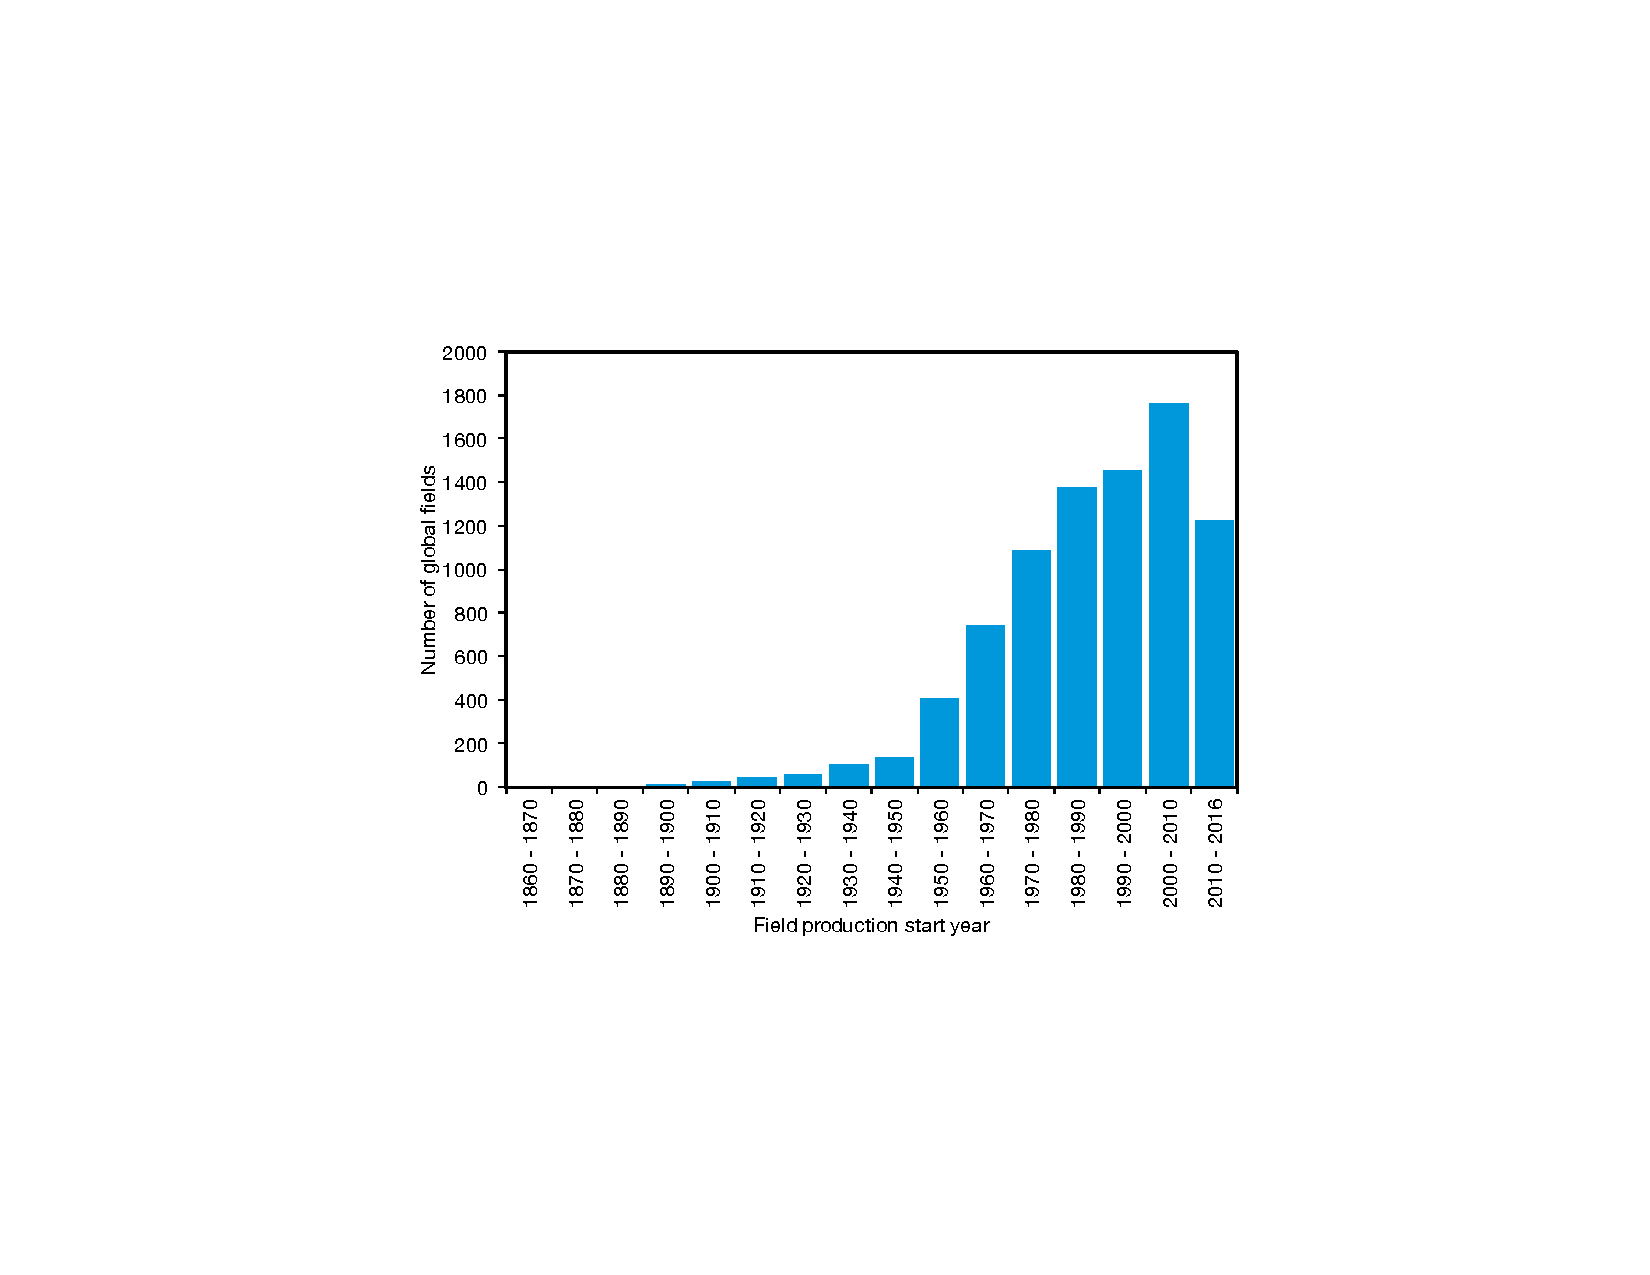
\includegraphics[width=0.85\columnwidth]{images/age_distribution_all.pdf}
\caption{Distributions of global oilfield ages.}
\label{fig:age_distribution_all}
\end{figure}

\begin{figure}[t]
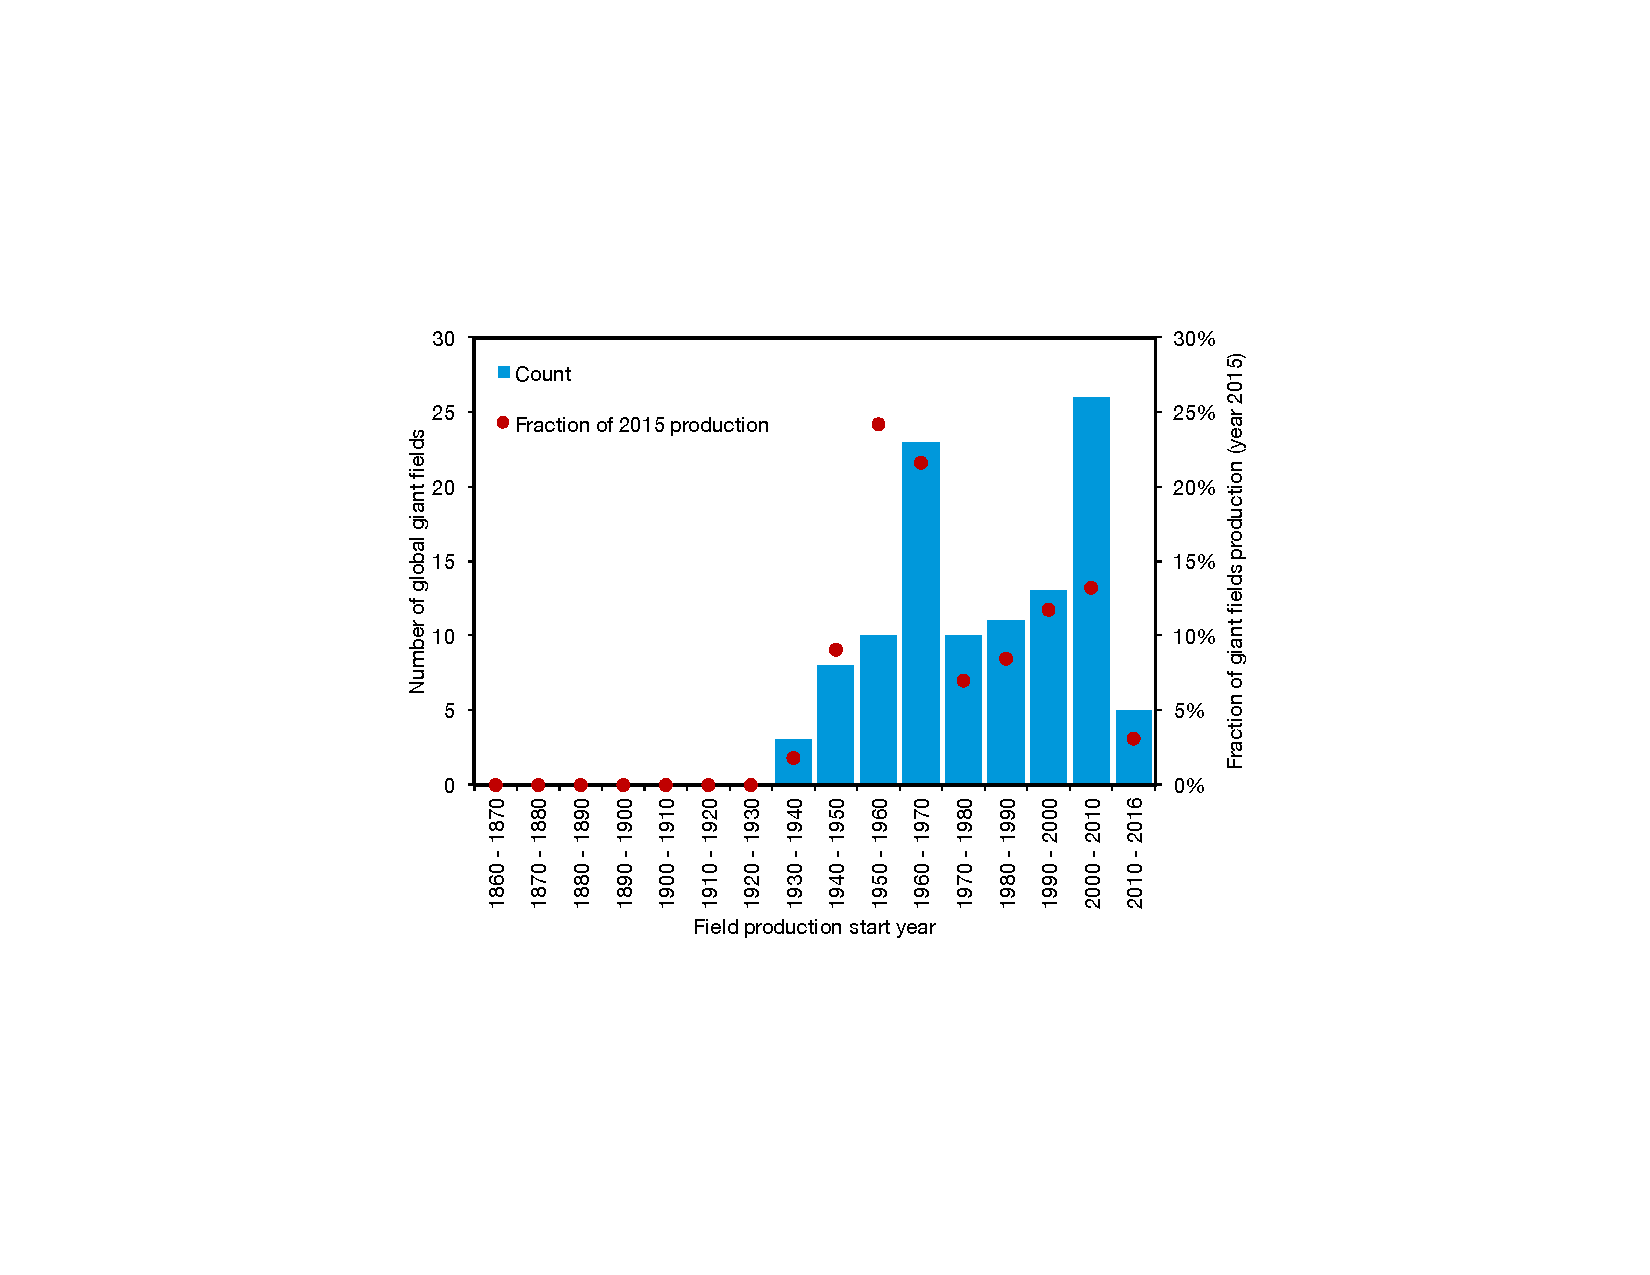
\includegraphics[width=0.85\columnwidth]{images/age_distribution_giant.pdf}
\caption{Distributions of giant oilfield ages.}
\label{fig:age_distribution_giant}
\end{figure}

\begin{table}
\begin{scriptsize}
\caption{Summary of oilfields age population data.}
\label{tab:oilfield_age}
\begin{tabular*}{0.8\columnwidth}{p{0.3\columnwidth}p{0.2\columnwidth}p{0.1\columnwidth}p{0.1\columnwidth}}
\toprule
Reference & Vol. W. Average & Median & SD \\
\midrule
All global oilfields & 1982 & 1991 & 21 \\
Giant oilfields & 1972 & 1980 & 22 \\
\bottomrule
\end{tabular*}
\end{scriptsize}
\end{table}
%TODO: Change smart default age to 2021-1980 = 41.




\subsection{Default field depth}

Field depth (\xlname{Field\_depth}) data were collected for a total of 7,344 global oilfields \cite{Masnadi2018}. For fields where a range of depths is presented, the mean of the range is used as a point estimate. The distribution of depths by number of fields per depth range is presented in in Figure \ref{fig:depth_distribution}. The mean depth for these fields is $\approx$7,122 ft (used as deterministic default) and the standard deviation (SD) is $\approx$3,851 ft. The depth distribution has a longer right tail (deep) than left tail (shallow), so the mean is somewhat larger than the median (6,654 ft).

\begin{figure}[t]
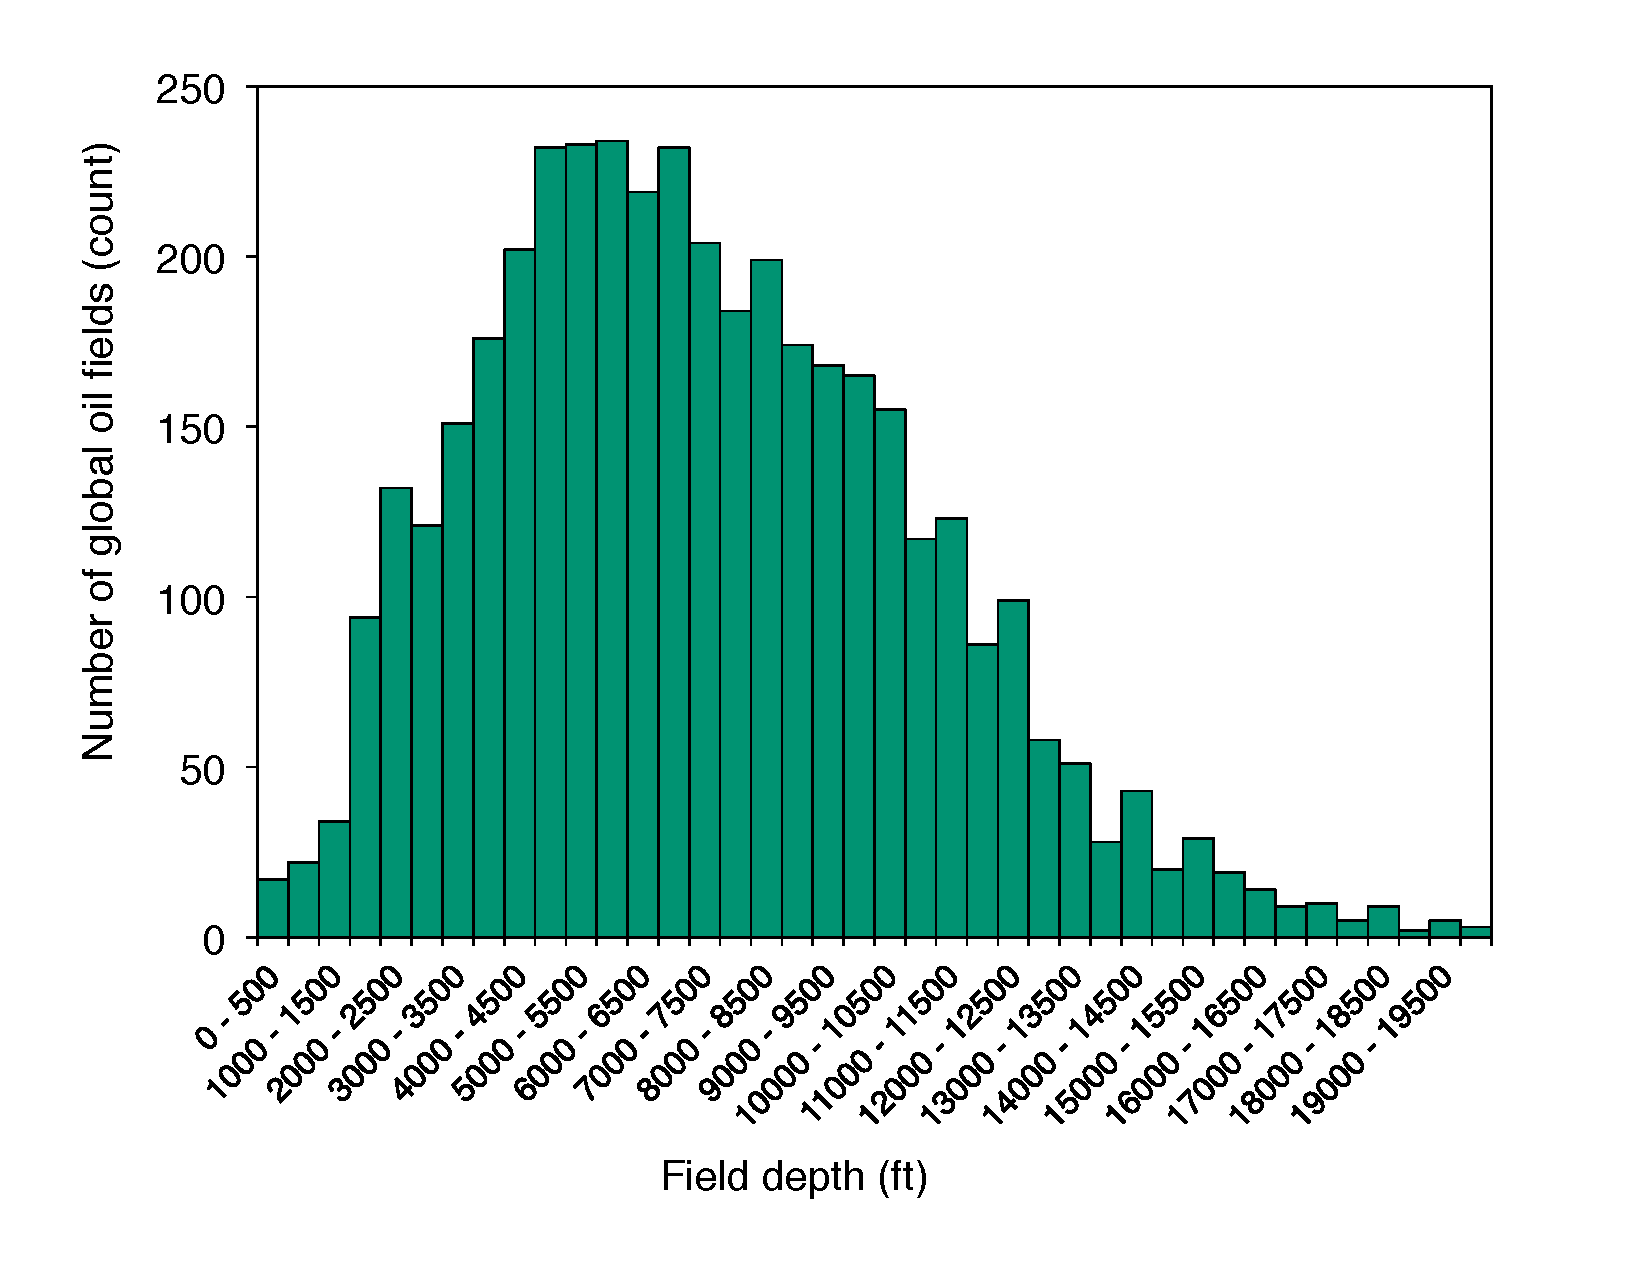
\includegraphics[width=0.8\columnwidth]{images/depth_distribution.pdf}
\caption{Distributions of global oilfield depths in bins of 500 ft depth.}
\label{fig:depth_distribution}
\end{figure}

\subsection{Default oil volumetric production}

In total, 5,070 global oilfields with available oil production data (\xlname{Oil\_prod}) are collected \cite{Masnadi2018}. As shown in Figure \ref{fig:production_distribution}, the majority of oilfields produce less than 250 bbl/d, with mean and SD of 2,098 and 2,445 bbl/d, respectively. 

\begin{figure}[t]
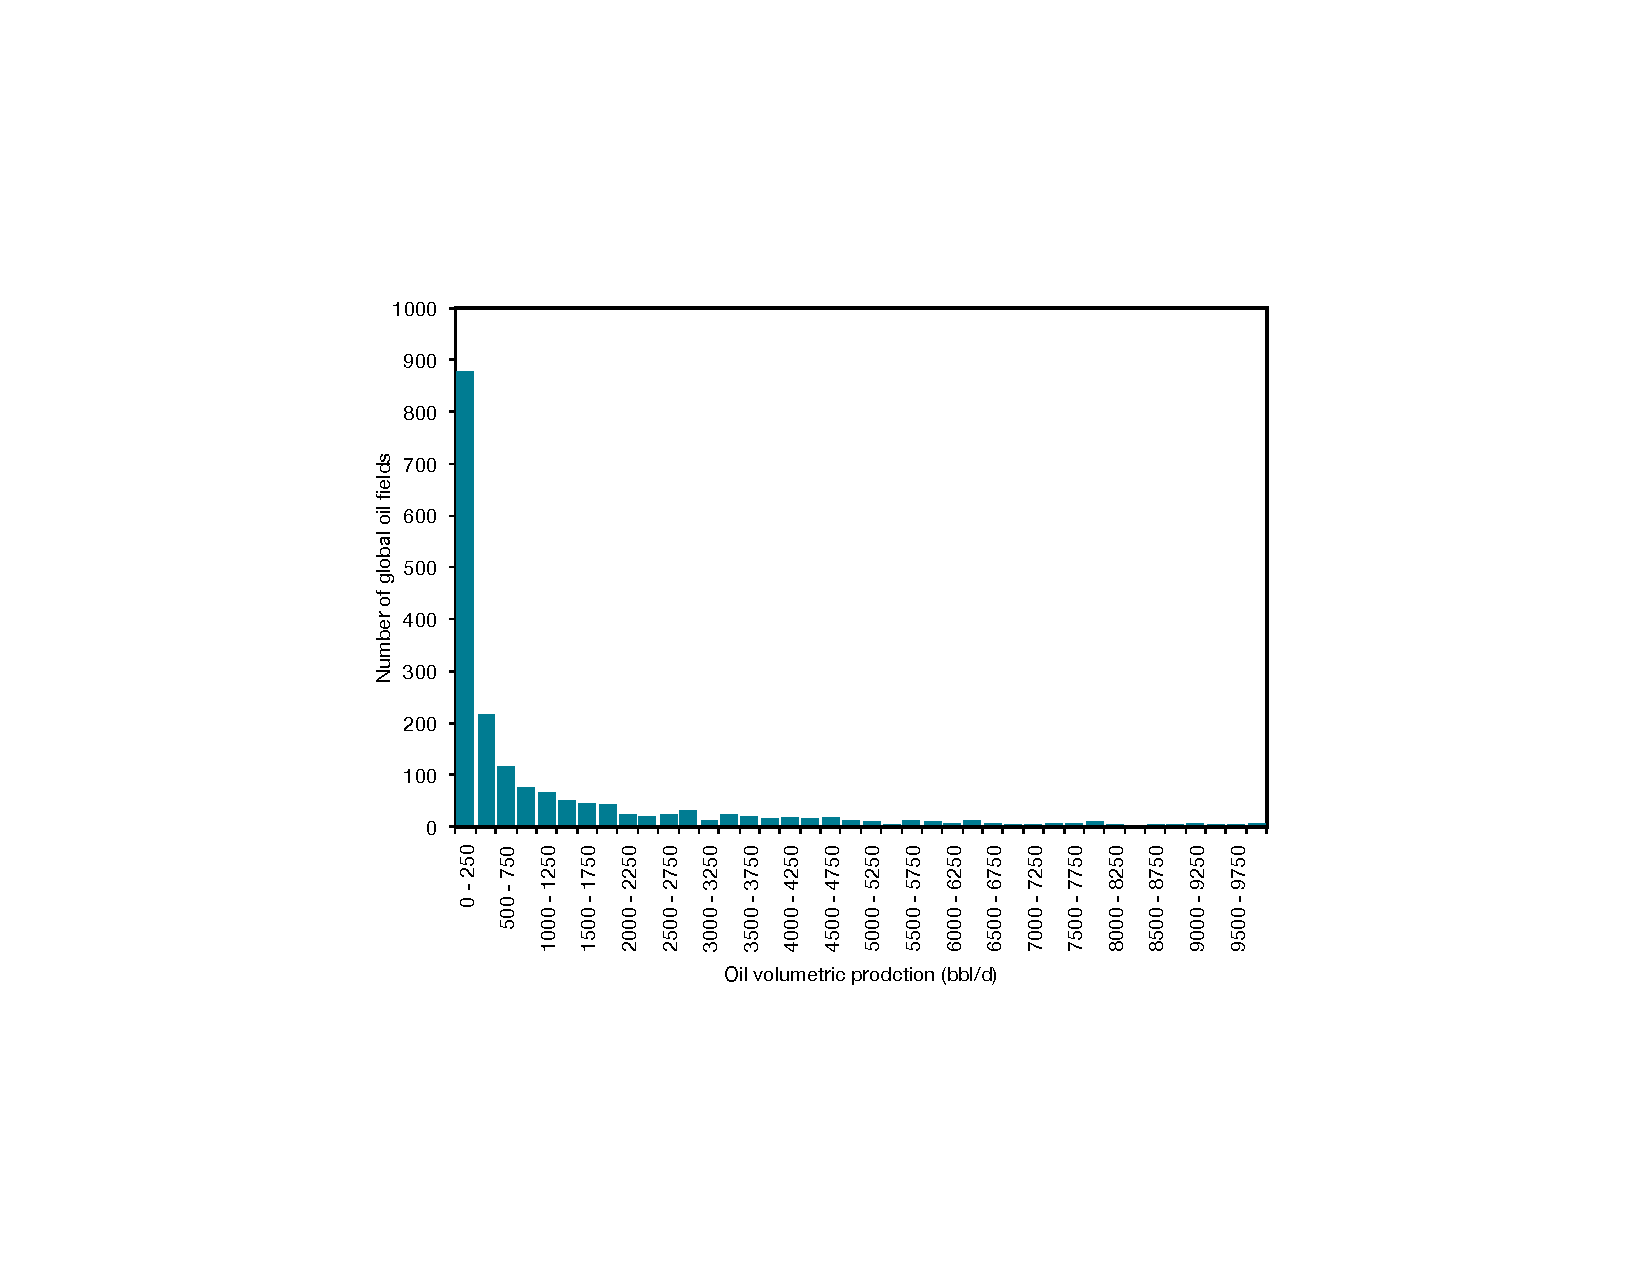
\includegraphics[width=0.8\columnwidth]{images/production_distribution.pdf}
\caption{Distributions of global oilfield daily volumetric oil production in bins of 250 bbl/d production.}
\label{fig:production_distribution}
\end{figure}

\subsection{Default production per well} \label{sec:well_production}

Country-level oil production data and numbers of producing wells were collected for a large number of oil producing countries. Data from a total of 106 oil producing countries were collected from the Oil \& Gas Journal \emph{2015 Worldwide Oil Field Production Survey} \cite{OGJ2015}. 

The distribution of per-well productivities for all countries is shown in Figure \ref{fig:productivity_distribution_all}. A majority of oil producing countries produced less than 500 bbl/well-d. Weighting these well productivities by country-level share of global production, we see a very similar distribution.

Because of the large number of countries producing less than 500 bbl/well-d, we plot the distribution for countries under 500 bbl/well-d (see Figure \ref{fig:productivity_distribution_low}). For the 61 countries with per-well productivity less than 500 bbl/well-d, the most common productivity by number of countries was the 0-25 bbl/well-d. However, when weighted by total production, the most common productivity bin is 75-100 bbl/well-d. An average productivity of 87.5 bbl/well-d is assumed as default well productivity in OPGEE. 

It is commonly known that the higher the field productivity index (PI, bbl/psi-d), the lower the number of producing wells and injectors. Based on the available data on the number of producing wells vs. the productivity index, the default number of producing wells is limited to 200 if the PI is higher than 6 bbl/psi-d. 

\begin{figure}[t]
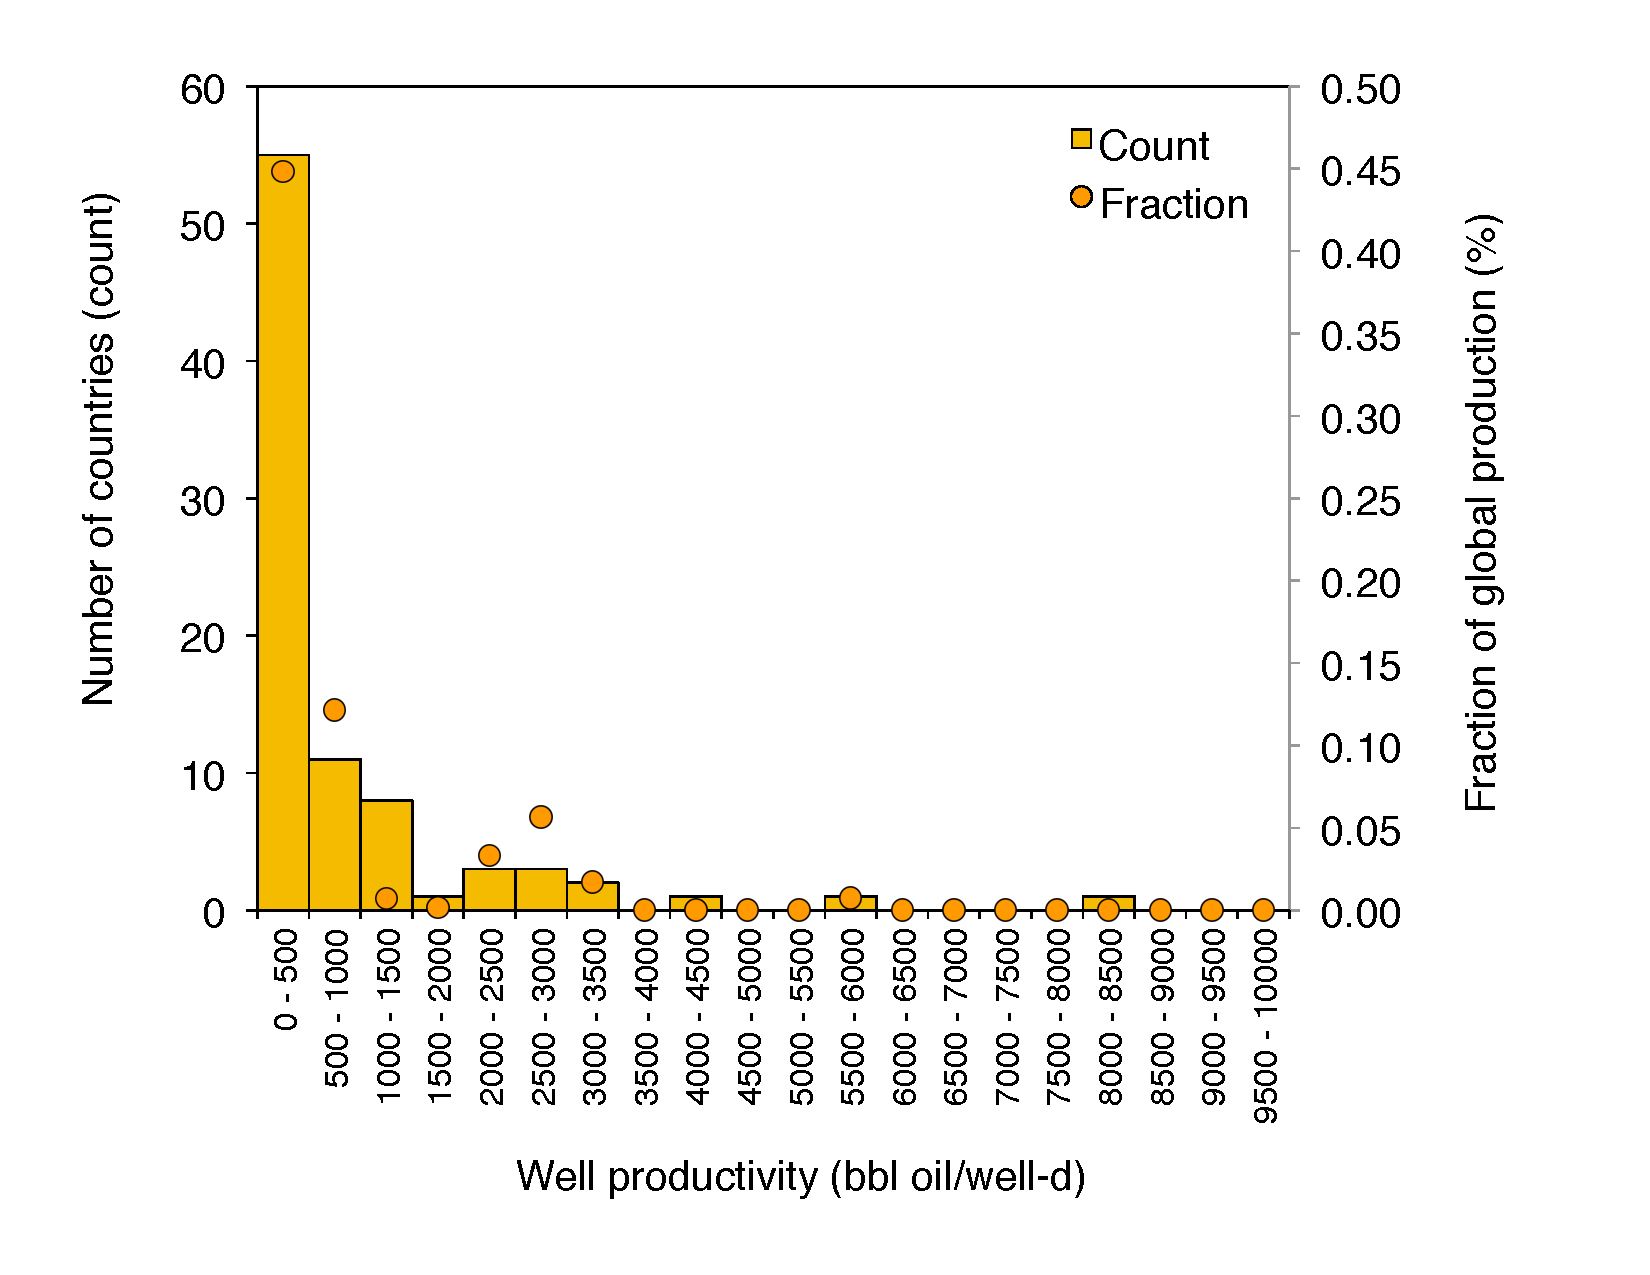
\includegraphics[width=0.8\columnwidth]{images/well_prod_all.pdf}
\caption{Distributions of oilfield per-well productivity (bbl oil/well-d) for bins of 500 bbl/d, counted by numbers of countries (bar) and by fraction of production (dot) $N$ = 106 countries.}
\label{fig:productivity_distribution_all}
\end{figure}

\begin{figure}[t]
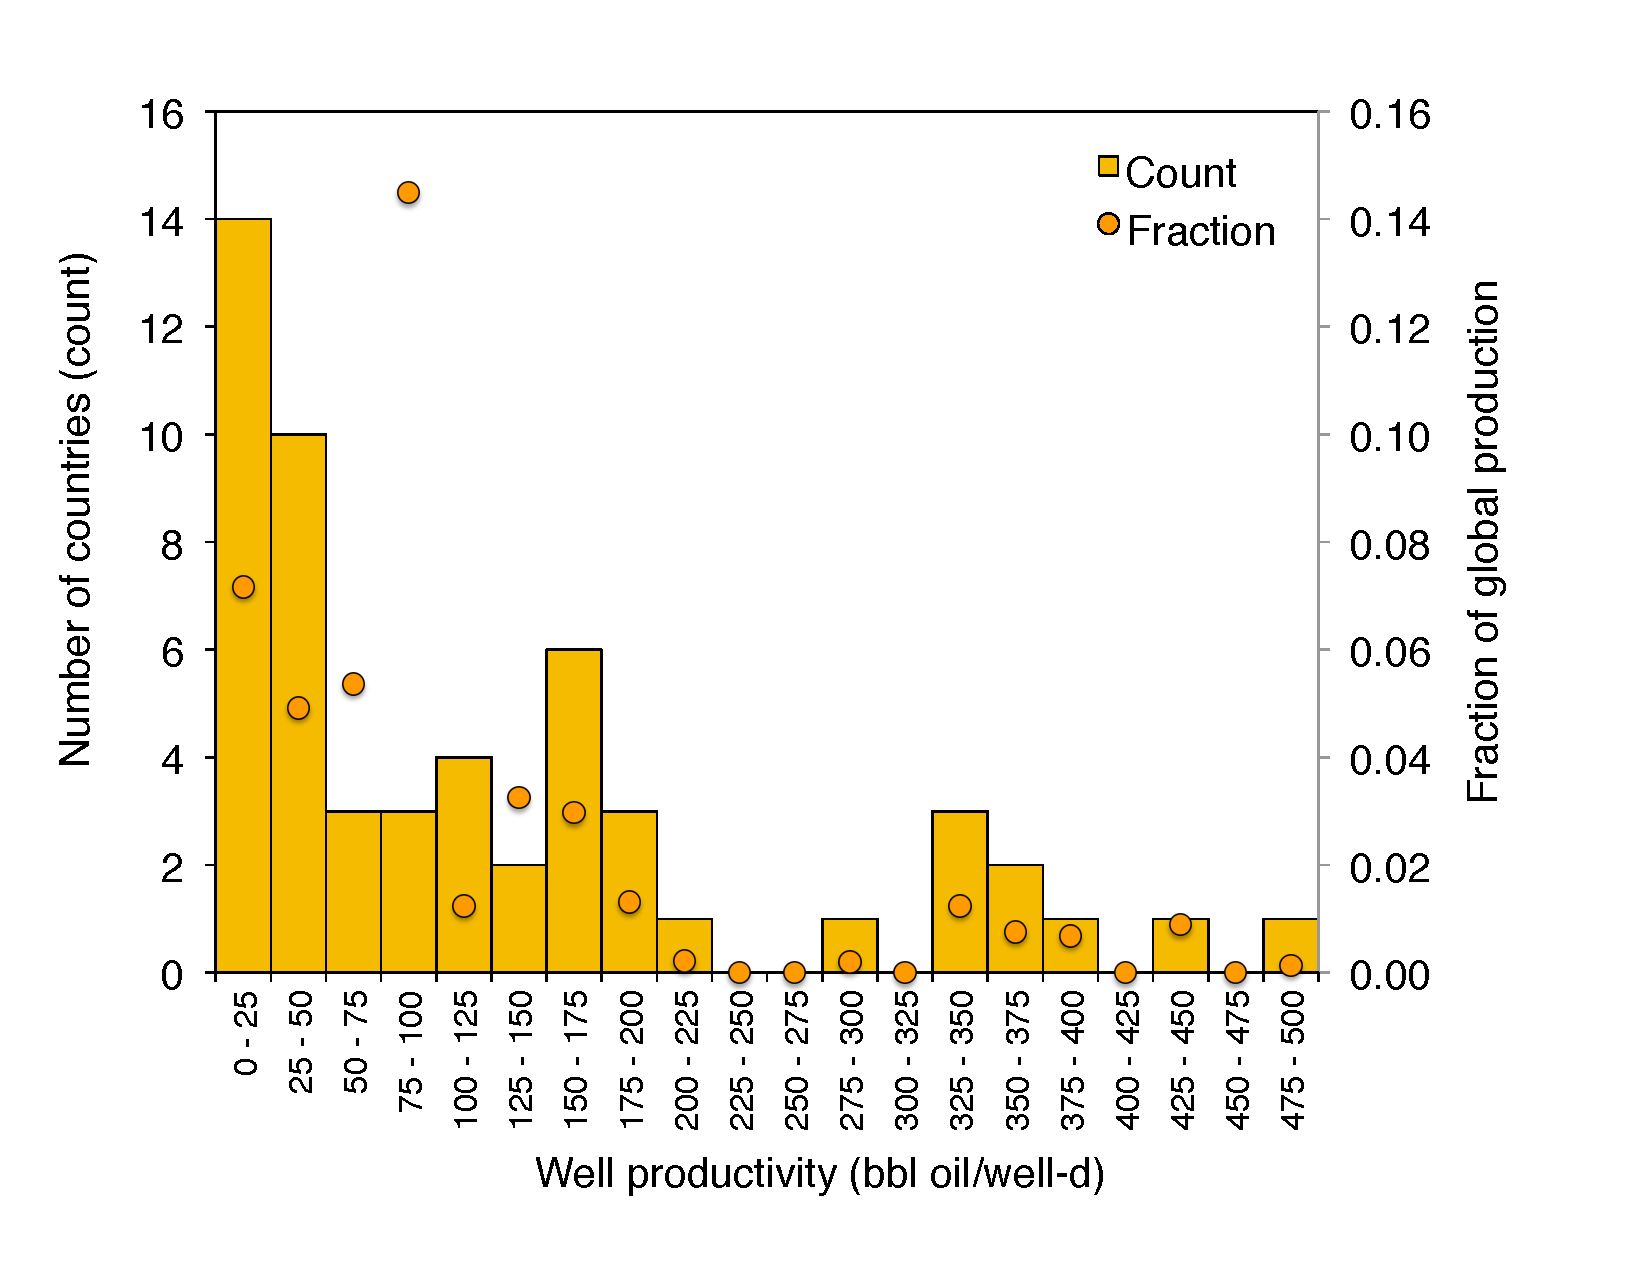
\includegraphics[width=0.8\columnwidth]{images/well_prod_low.pdf}
\caption{Distributions of oilfield per-well productivity (bbl oil/well-d) for all countries with per-well productivities lower than 500 bbl/well-d, counted by numbers of countries (bar) and by fraction of production (dot) $N$ = 61 countries.}
\label{fig:productivity_distribution_low}
\end{figure}

\subsection{Default number of injector wells}

The default number of injector wells (\xlname{Num\_water\_inj\_wells}) is a smart default based on the number of producing wells. To model this relationship, data from California, Alaska, and a variety of offshore fields from Canada, Nigeria, Norway and U.K. (206 fields in total) was collected \cite{DOGGR2011, AOGCC2012a}. Data from some of the offshore fields is provided in Table \ref{tab:offshore_inj_prod} below. Per-well productivity across these fields ranges from less than 10 bbl/d to over 10,000 bbl/d.

A strong relationship is seen between the productivity of producing wells and the number of injection wells required. Highly productive wells require a significantly larger number of injectors. Figure \ref{fig:inj_prod} shows the relationship between the per-well productivity of a field and the ratio of injectors to producers. Figure \ref{fig:inj_prod_hist} also shows the ratio of injectors to producers histogram that is not normally distributed. From these data, a relationship was generated for the mean and median ratio for each logarithmic bin of production well productivity (see Table \ref{tab:inj_prod_ratios}). Median values for each bin are used to define the smart default for the number of injector wells.

\begin{table}
\begin{scriptsize}
\caption{Mean and median injector to producer ratios.}
\label{tab:inj_prod_ratios}
\begin{tabular*}{0.8\columnwidth}{p{0.3\columnwidth}p{0.1\columnwidth}p{0.1\columnwidth}p{0.1\columnwidth}}
\toprule
Prod. well productivity & Mean & Median & SD \\
\midrule
0-10 bbl/d & 0.1957 & 0.143 & 0.167 \\
10 - 100 bbl/d & 0.338 & 0.267 & 0.259 \\
100 - 1000 bbl/d & 0.556 & 0.512 & 0.281 \\
$>$ 1000 bbl/d & 0.715 & 0.829 & 0.287 \\
\bottomrule
\end{tabular*}
\end{scriptsize}
\end{table}


\begin{figure}[t]
\includegraphics[width=0.8\columnwidth]{images/inj_prod.pdf}
\caption{Ratio of producers to injectors as a function of per-well productivity of 206 fields. Source: Various.}
\label{fig:inj_prod}
\end{figure}

\begin{figure}[t]
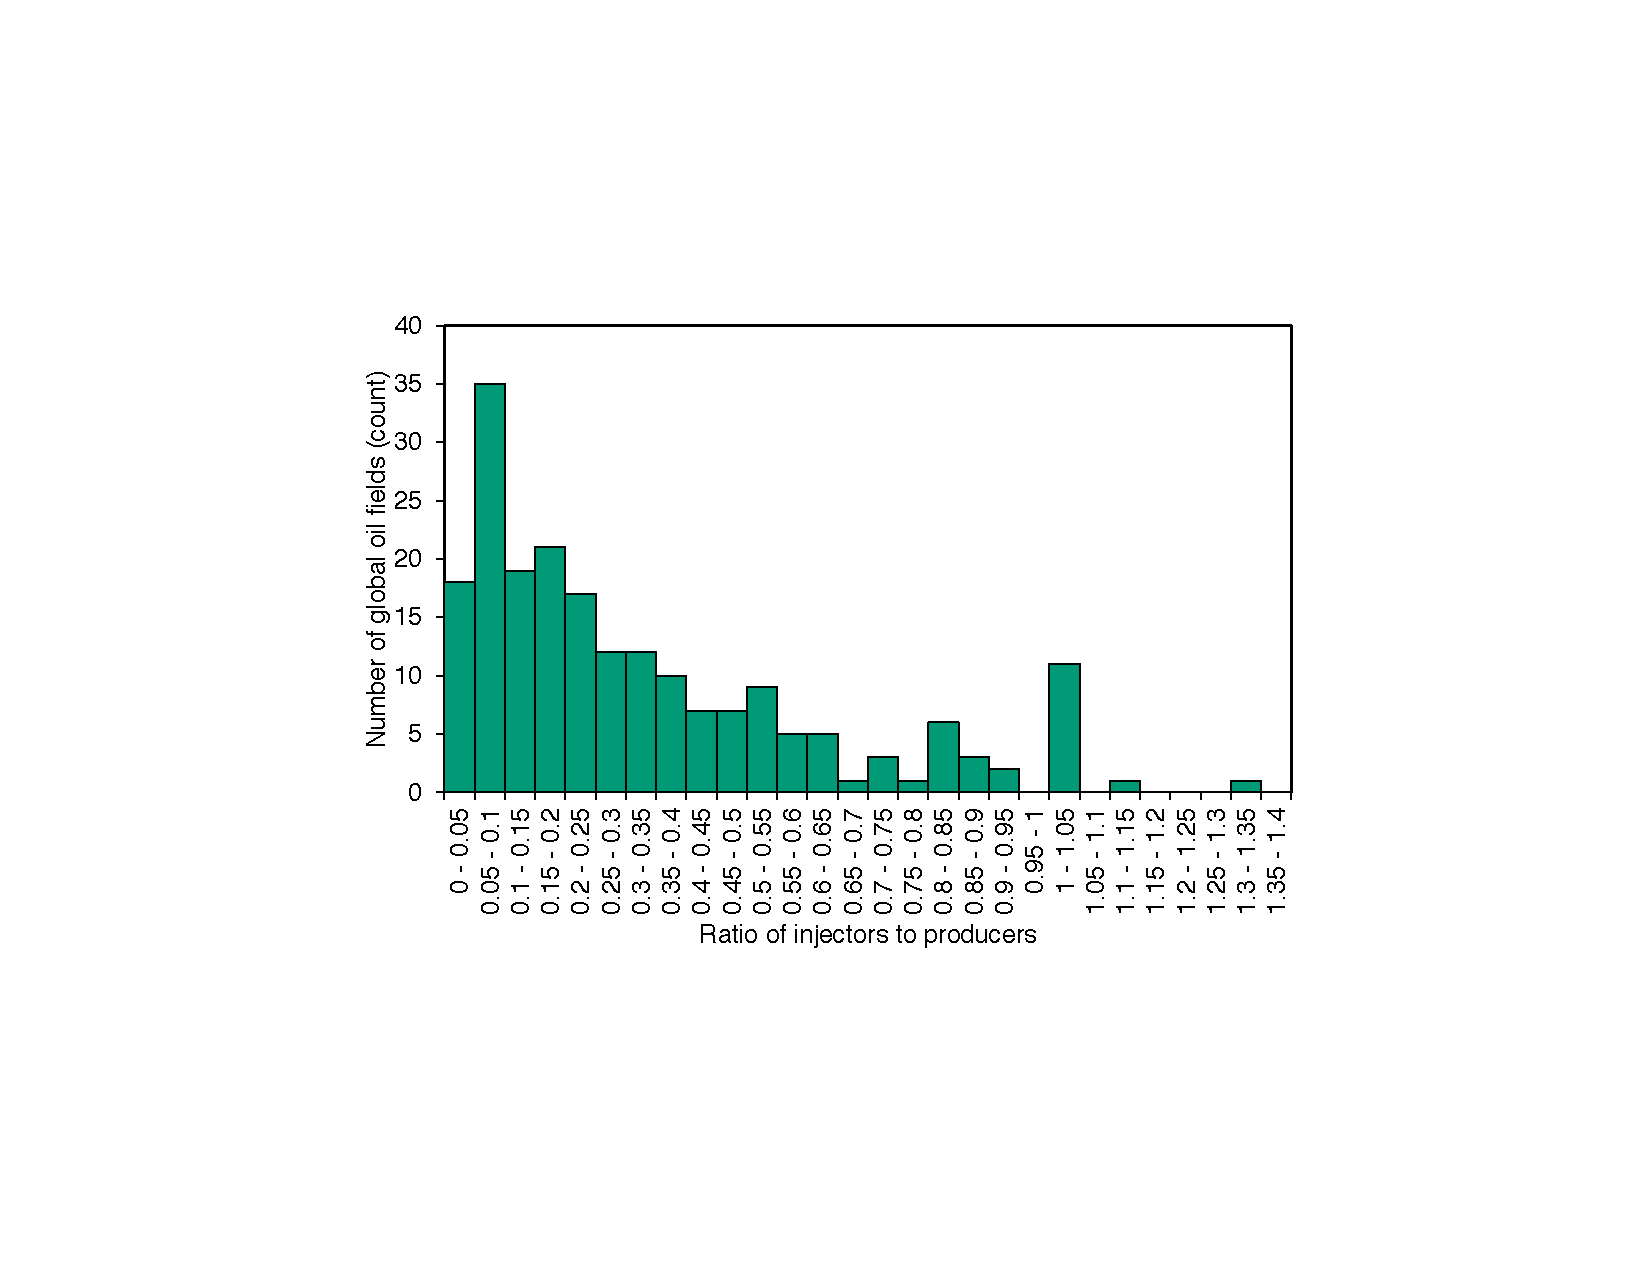
\includegraphics[width=0.8\columnwidth]{images/inj_prod_hist.pdf}
\caption{Distribution of the ratio of injectors to producers of 206 global oilfields.}
\label{fig:inj_prod_hist}
\end{figure}

\begin{landscape}
\begin{table}
\begin{scriptsize}
\caption{Data on production, number of production wells, and number of injection wells by offshore field.}
\label{tab:offshore_inj_prod}
\begin{tabular*}{1\columnwidth}{p{0.1\columnwidth}p{0.03\columnwidth}p{0.03\columnwidth}p{0.05\columnwidth}p{0.65\columnwidth}}
\toprule
Field & Prod. wells &Inj. wells & Prod. (bbl/d) &References \\
\midrule
Dalia &37 &31 &240000 &\url{http://www.offshore-technology.com/projects/dalia/} \\
Gimboa &3 &4 &14000 &\url{http://www.statoil.com/en/OurOperations/TradingProducts/CrudeOil/Crudeoilassays/PagPa/Gimboa.aspx}
\url{http://www.offshore-technology.com/projects/gimboa/} \\
Girassol &23 &13 &240000 &\url{http://www.offshore-technology.com/projects/girassol/} \\
Plutonio &20 &20 &240000 &\url{http://www.offshore-technology.com/projects/greater_plutonio/} \\
Hungo &30 &26 &130000 &\url{http://www.exxonmobil.com/crudeoil/about_crudes_hungo.aspx}
\url{http://www.fluor.com/projects/Pages/ProjectInfoPage.aspx?prjid=93} \\
Kissanje &25 &21 &150000 &\url{http://www.exxonmobil.com/crudeoil/about_crudes_kissanje.aspx} 
\url{http://www.ogj.com/articles/print/volume-103/issue-38/special-report/kizomba-b-attains-production-capacity-early.html} \\
Mondo &17 &17 &65000 &\url{http://www.exxonmobil.com/crudeoil/about_crudes_mondo.aspx}
\url{http://www.offshore-technology.com/projects/kizomba/} \\
Pazflor &25 &22 &220000 &\url{http://www.exxonmobil.com/crudeoil/about_crudes_pazflor.aspx}
\url{http://www.ship-technology.com/projects/pazflor-fpso/} \\
Azeri &58 &25 &823000 &\url{http://crudemarketing.chevron.com/crude/central_asian/azeri.aspx}
\url{http://www.bp.com/genericarticle.do?categoryId=9029616&contentId=7067613} \\
Albacora Leste &16 &14 &180000 &Albacora Leste Field Development Project, Offshore Technology Conference, 2006 (OTC 17925) \\
Bijupira &9 &6 &70000 &\url{http://www.offshore-technology.com/projects/bijupira/} \\
Frade &11 &4 &65000 &\url{http://www.offshore-technology.com/projects/fradefieldcamposbasi/} \\
Jubarte &20 &7 &180000 &\url{http://www.epcengineer.com/}
\url{http://subseaiq.com/data/Project.aspx?project_id=764&AspxAutoDetectCookieSupport=1} \\
Lula &5 &2 &100000 &\url{http://subseaiq.com/data/Project.aspx?project_id=274} \\
Marlim &102 &50 &390000 &\url{http://www.offshore-technology.com/projects/marlimpetro/} \\
Marlim Sul &41 &34 &300000 &\url{http://uk.reuters.com/article/2011/06/02/petrobras-platform-idUKN0227875420110602} 
\url{http://subseaiq.com/data/Project.aspx?project_id=371} \\
Polvo &10 &3 &30000 &\url{http://www.offshore-mag.com/articles/print/volume-68/issue-3/production-operations/devon-breaks-new-ground-at-polvo.html} \\
Roncador &40 &24 &460000 & \url{http://subseaiq.com/data/Project.aspx?project_id=348} \\
Sapinhoa &10 &10 &120000 & \url{http://www.offshore-technology.com/projects/guaraoilfield/} \\
\bottomrule
\end{tabular*}
\end{scriptsize}
\end{table}
\end{landscape}

\subsection{Default well diameter}
The well diameter parameter refers to the production tubing diameter. It is uncommon for a production tubing diameter (\xlname{Well\_diam}) to be over 5 inch (some highly productive wells in Middle East region excepted). Therefore, a triangularly distributed default well diameter with 1 to 5 inch range is defined in OPGEE. The OPGEE default diameter is 2.78 inches.   

\subsection{Default productivity index}
An oilfield's productivity index (PI)(\xlname{Prod\_index}) is an important OPGEE input parameter, as field PI directly affects the productivity of wells. However, \emph{PI} data are rarely reported in the literature. Masnadi et al. \cite{Masnadi2018} found a total of 11 datapoints of reported PI in their literature search.

To remedy this, the Wood MacKenzie dataset used in Masnadi et al. \cite{Masnadi2018}  was accessed for fields with key related parameters. Data from all fields was filtered to include fields with reported data on permeability and net pay thickness. A total of 3453 fields contain permeability data. Of these fields, a total of 366 contain both permeability and net pay thickness, two key determinants of PI. 

In order to model PI, The steady-state radial inflow model is assumed to apply \cite[Ch. 3]{Guo2019}. In addition to permeability and net pay thickness, the steady-state radial inflow model requires data on the following: (1) oil formation volume factor $B_o$ [reservoir bbl/stock tank bbl], (2) oil viscosity $\mu_o$ [cp], (3) the radius of the wellbore sand face  $r_w$ [ft] (4) the radius of the far-field constant pressure boundary, $r_e$ [ft], and (5) the skin factor $S$ [-]. For simplicity, $B_o$ is assumed to be = 1.3 for all fields, $r_w$ = 0.33 ft, $r_e$ = 1000 ft. 

Viscosity of crude is estimated using the classical Beggs and Robinson viscosity relationship for dead oil viscosity \cite{PengTools2021}. This relationship requires crude oil API gravity (available for all fields in WM dataset) and temperature. Temperature is used where available in dataset, or estimated using depth and geothermal gradient of 25 $^\circ$C per km increase from surface temperature of 15$^\circ$C.

The resulting distribution of PIs is given in Figure \ref{fig:PIdist}. The mean PI in the dataset is 6.85 bbl/psi-d. The production-weighted mean is 10.13 bbl/psi-d.


\begin{figure}
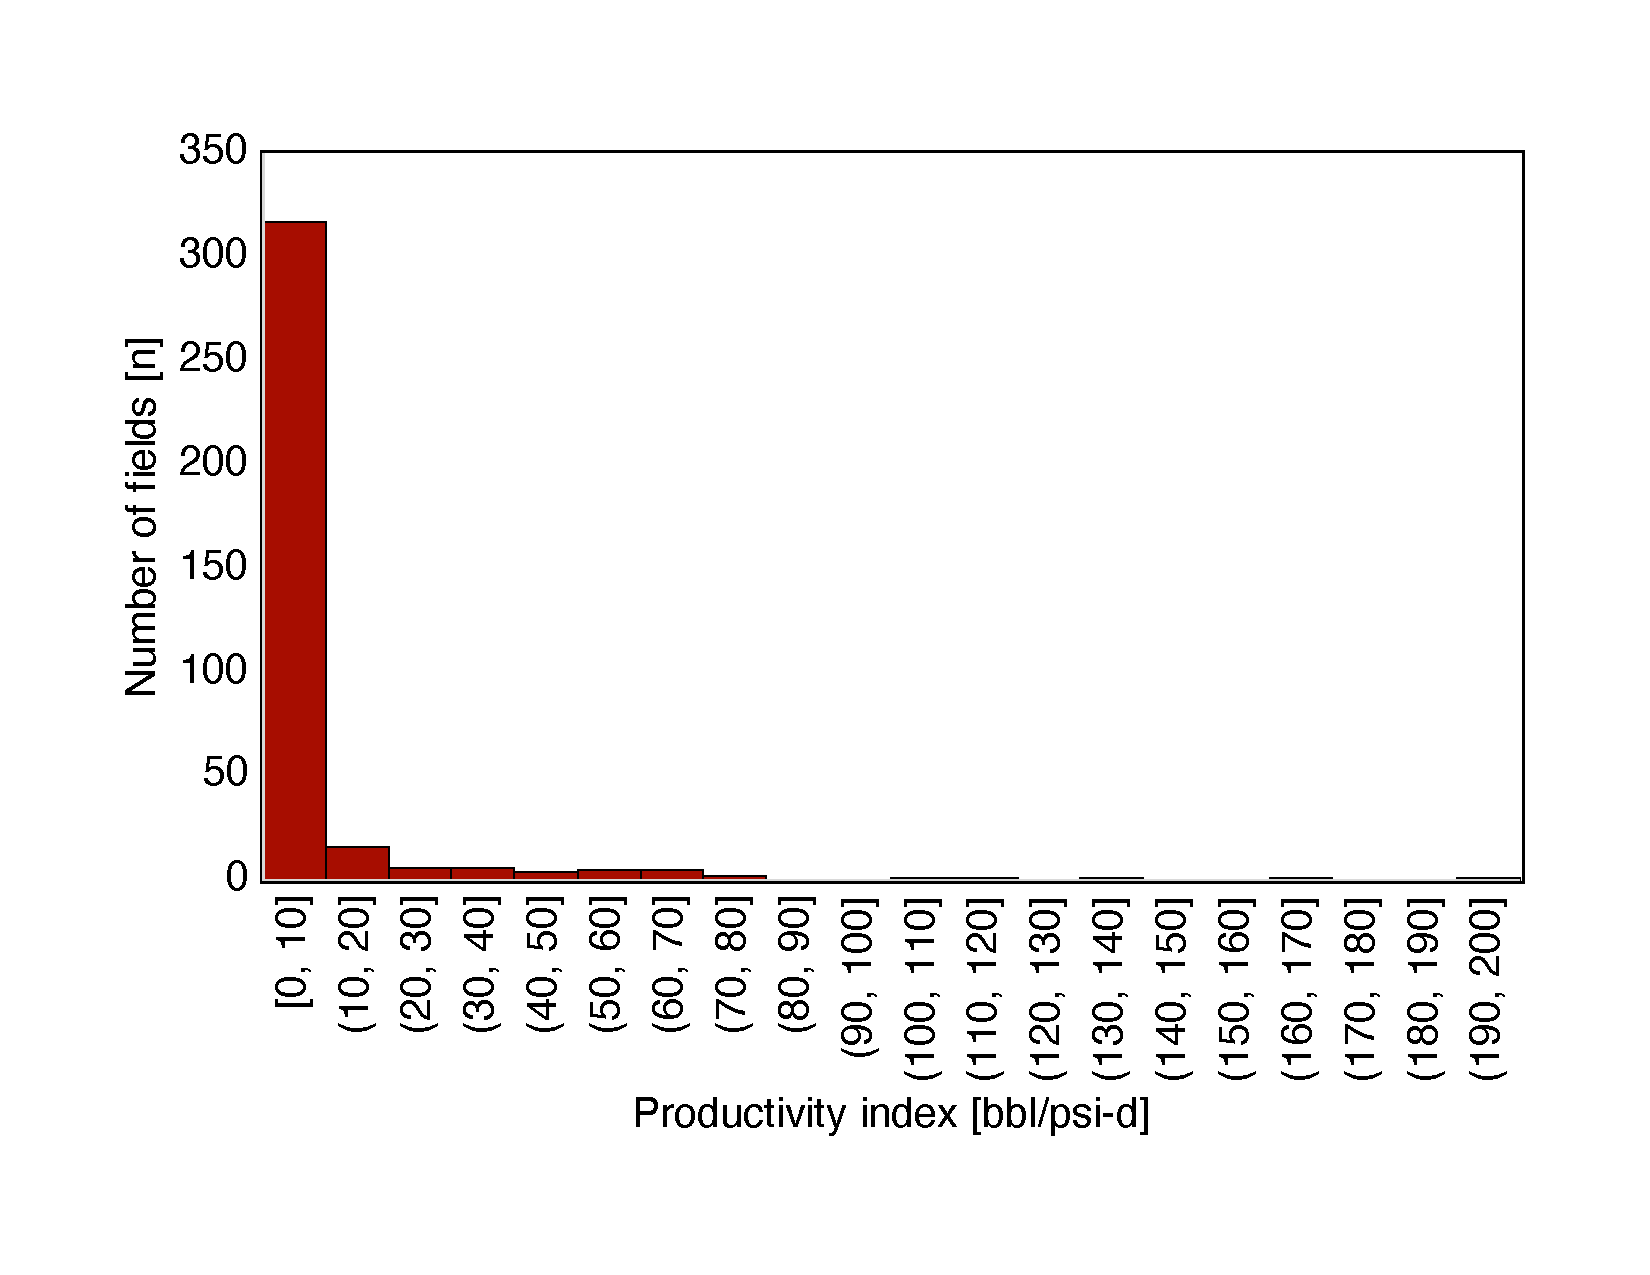
\includegraphics[width=0.8\columnwidth]{images/ProdIndexDist.pdf}
\caption{Distribution of productivity index (PI) [bbl/psi-d] for 366 fields.}
\label{fig:PIdist}
\end{figure}



\subsection{Default reservoir pressure}
The reservoir pressure (\xlname{Res\_press}) is calculated based on a multiplication of a coefficient $\alpha (t)$ (a function of reservoir age, \emph{t}) to the default initial reservoir pressure. The default reservoir pressure is assumed to be the hydrostatic pressure, or the pressure in the reservoir fluids necessary to sustain a column of water to the surface \cite{fertl1981abnormal}. 

%%%%%%%%%%
\begin{minipage}{0.6\columnwidth} \label{eq:res_pressure1}
\begin{fleqn}[0pt]
\begin{equation}
p_{R}= \alpha D_{w}/2.31 \quad\quad\eqnunit{psia}
\end{equation}
\end{fleqn}
\end{minipage}\hfill
\begin{minipage}{0.3\columnwidth}
        \begin{tabular}{|cl}
        & \\
        $p_{R}$   & \xlname{Res\_press}\\
        $D_{w}$   & \xlname{Field\_depth}\\
        & \\
        \end{tabular}
\end{minipage}
%%%%%%%%%%
where \xlname{Field\_depth} is the reservoir depth (ft). In order to find a relationship for $\alpha$, (2.31*\xlname{Res\_press}/\xlname{Field\_depth}) of several offshore and onshore global fields are plotted as a function of field age. Minimizing the square of residuals, different functions (i.e. exponential, logarithmic, polynomial, and power) are examined to find the best fit: 

%%%%%%%%%%
\begin{minipage}{0.6\columnwidth} \label{eq:res_pressure2}
\begin{fleqn}[0pt]
\begin{equation}
\alpha=4.9*10^{-8}t{^2}+0.95 \quad\quad\eqnunit{s}
\end{equation}
\end{fleqn}
\end{minipage}\hfill
\begin{minipage}{0.3\columnwidth}
        \begin{tabular}{|cl}
        & \\
        $t$   & \xlname{Field\_age}\\
        & \\
        \end{tabular}
\end{minipage}
\begin{equation}
\end{equation}
%%%%%%%%%%

\subsection{Default reservoir temperature}
Reservoir temperature (\xlname{Res\_temp}) is also a direct function of the reservoir depth. Reservoir temperature can be estimated base on the following expression:

%%%%%%%%%%
\begin{minipage}{0.6\columnwidth}\label{eq:res_temp}
\begin{fleqn}[0pt]
\begin{equation}
T_{R}=T_{a}+\Delta T\cdot D_{w}/100 \quad\quad\eqnunit{$^{\circ}$F}
\end{equation}
\end{fleqn}
\end{minipage}\hfill
\begin{minipage}{0.3\columnwidth}
        \begin{tabular}{|cl}
        & \\
        $T_{R}$   & \xlname{Res\_temp}\\
        $D_{w}$   & \xlname{Field\_depth}\\
        & \\
        \end{tabular}
\end{minipage}
%%%%%%%%%%
where $T_{R}$ and \emph{T$_{a}$} are reservoir and ambient temperatures, respectively. A geothermal gradient of 1.8$^{\circ}$ per 100 ft is assumed. 

\subsection{Default API gravity}

The API gravity (\xlname{API\_grav}) of 7,223 global oilfields have been obtained \cite{Masnadi2018}. The histogram shown in Figure \ref{fig:API} reveals that the majority of global fields lie within 35-40 $^\circ$API with an average of 32.8 $^\circ$API and a SD of 8.4 $^\circ$API.  

\begin{figure}
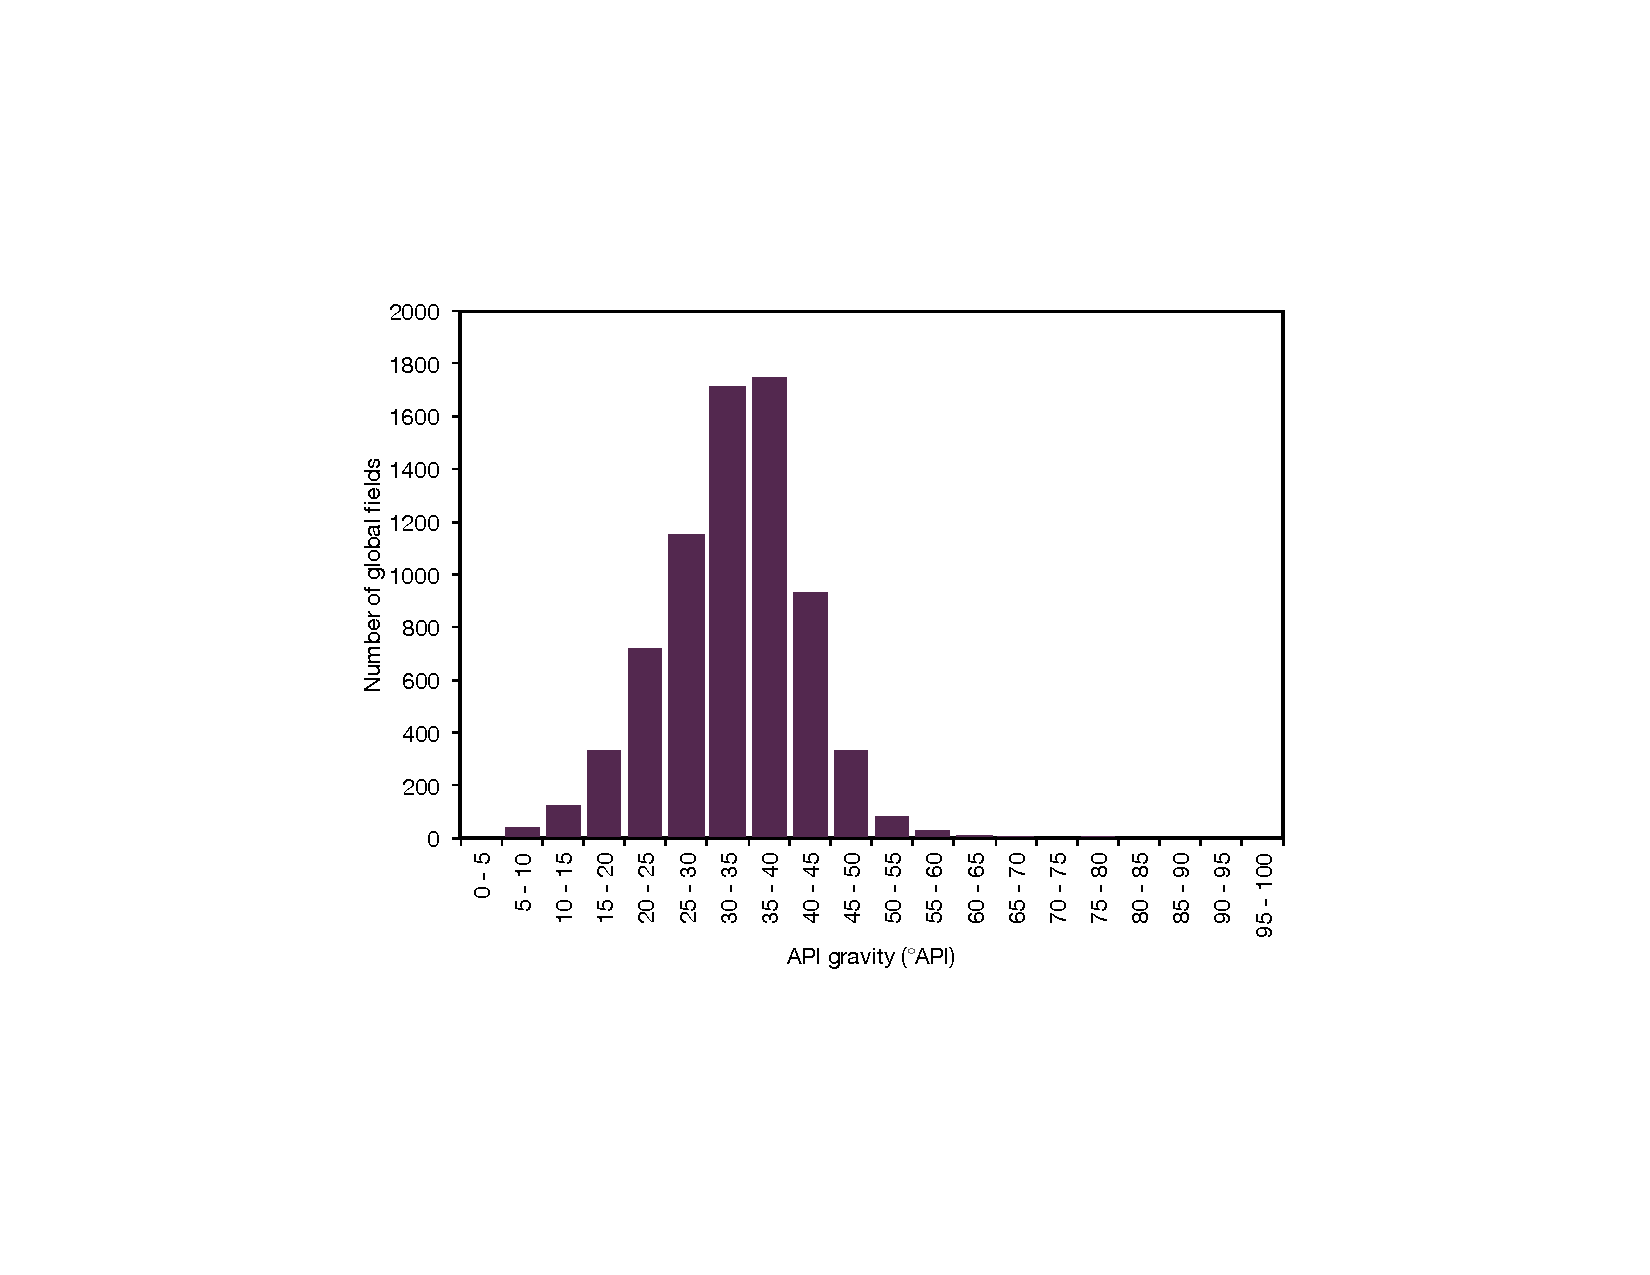
\includegraphics[width=0.8\columnwidth]{images/API.pdf}
\caption{The API gravity distribution of 7,223 global oilfields for bins of 5 $^\circ$API.}
\label{fig:API}
\end{figure}

\subsection{Default gas composition}

All gas species except for CO$_2$ are based on analysis by the National Energy Technology Laboratory \cite{Littlefield2019} of the US Geological Survey's Energy Geochemistry Laboratory Database (EGDB). Basin-specific gas composition data (mass fractions) (sourced from Report Exhibit 3-2 pp. 13-14) were converted to volume fractions and a US average was calculated by weighting according to basin-level gas production. 

For CO$_2$ concentration, the overall global OPGEE default gas composition uses values entirely based upon the NETL analysis of the USGS database. This results in CO$_2$ mole fraction of 0.3\%. This dataset is used for the global OPGEE default because it includes more samples than other known databases.

However, it is known that fields that supply California tend to have higher CO$_2$ fraction than present in the broader USGS database. The LCFS default, instead, uses a CO$_2$ mole fraction computed based on shares of crude oil supply to California. 

For California-specific production, the CO$_2$ content of associated gas from oil production is derived from reported gas composition data from 135 California oil fields \cite{Lee2011}. Species concentration distributions for major gas species is shown in Figure \ref{fig:gas_comp_major}. In order to remove outliers, all compositions with methane concentration less than 50\% were removed from the dataset (17 data points removed out of 135). The resulting mean compositions were rounded to the nearest \%. These values were used as the OPGEE default in OPGEE v2.0.

For the 75\% of crude supplied to California but not sourced in California, data were gathered from various sources. Wood Mackenzie data on CO$_2$ content of LCFS source countries was averaged for all reporting fields in each importing country.  For Ecuador, values from Masnadi et al. were used \cite{Masnadi2018}. For Alaska, Wood MacKenzie data were used for Alaska fields. For the remainder of US fields, the average of all other (non-California, non-Alaska) samples was used (0.2\% CO$_2$, similar to USGS). For countries with no CO$_2$ concentrations included in Wood MacKenzie, the average CO$_2$ fraction of all global Wood MacKenzie fields is used. This procedure results in a volume weighted average CO$_2$ content of California-supplying fields of 6.9 mol\%.

In order to allow mass balance to hold, all other gases in the case of the LCFS default are adjusted downward proportionally to allow mole fractions to sum to 100\%. The resulting default gas compositions are given in Table \ref{tab:gas_composition}.


\begin{figure}
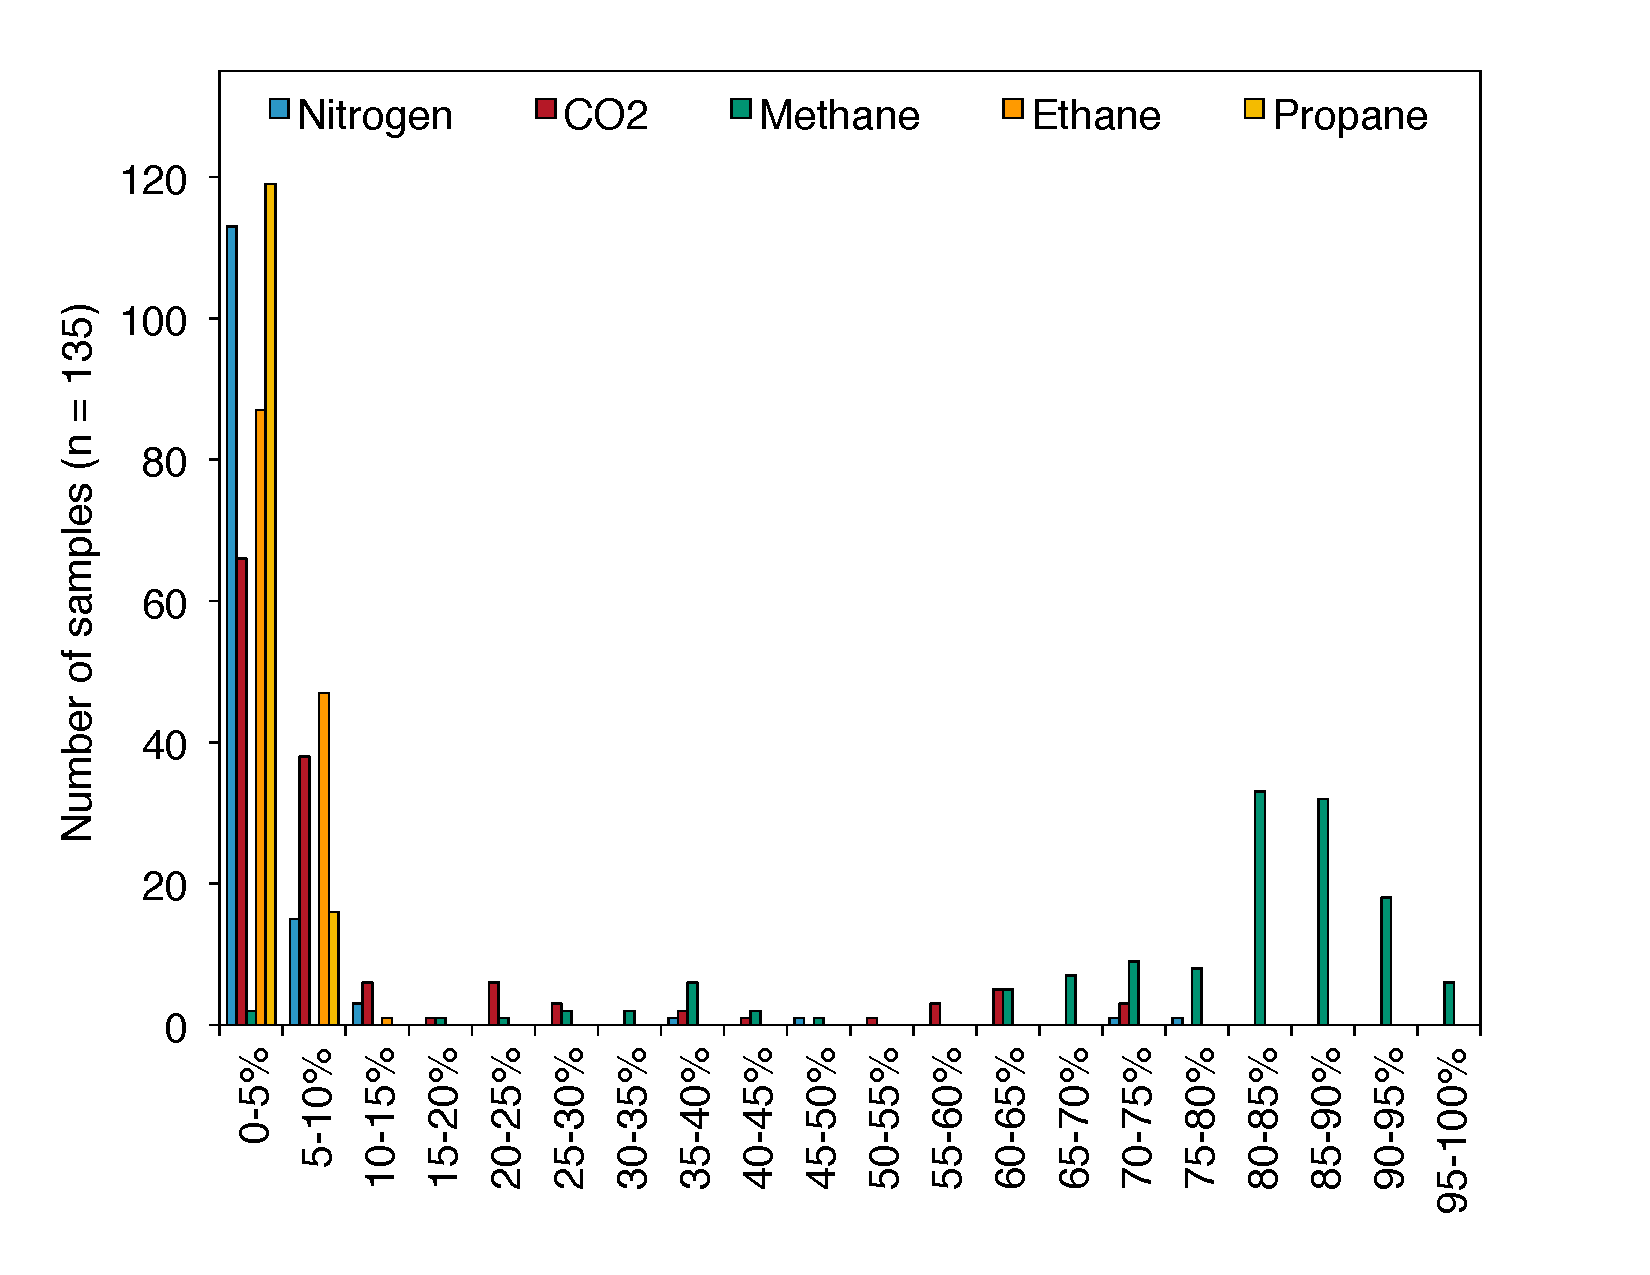
\includegraphics[width=0.8\columnwidth]{images/gas_comp_major.pdf}
\caption{Distributions of major gas species across 135 samples from California associated gas producers.}
\label{fig:gas_comp_major}
\end{figure}

\begin{table}
\begin{scriptsize}
\caption{Gas composition for overall OPGEE default and California LCFS default}
\label{tab:gas_composition}
\begin{tabular*}{0.5\columnwidth}{p{0.1\columnwidth}p{0.15\columnwidth}p{0.15\columnwidth}}
\toprule
Species & LCFS mole \% & Global mole \%  \\
\midrule
N$_2$	&2.7		& 2.9 \\
CO$_2$	&6.9		& 0.3 \\
C$_1$	&83.3	& 89.2 \\
C$_2$	&4.9		& 5.3 \\
C$_3$	&1.5		& 1.6 \\
C$_4+$	&0.7		& 0.7 \\
H$_2$S	&0.0		& 0.0 \\
\bottomrule
\end{tabular*}
\end{scriptsize}
\end{table}

\subsection{Default GOR} \label{sec:GOR_default}

The gas-oil ratio (GOR, \xlname{GOR}) varies over the life of the field. The amount of gas able to be evolved from crude oil depends on its API gravity, the gas gravity, and the temperature and pressure of the crude oil \cite[p. 297]{Mccain1990}. As the reservoir pressure drops, increasing amounts of gas evolve from the liquid hydrocarbons (beginning at the bubble point pressure if the oil is initially undersaturated) \cite{Mccain1990}. This tends to result in increasing producing GOR over time. Also, lighter crude oils tend to have a higher GOR. 

Because of this complexity, a static single value for GOR is not desirable. However, all data required to use empirical correlations for GOR is not likely to be available for all crude oils modeled. We obtained GOR data of 3,161 global oilfields \cite{Masnadi2018}. 

Crude oils are binned by API gravity into heavy ($<$ 20 $^\circ$API), medium ($\geq$ 20, $<$ 30 $^\circ$API), and light crude ($\geq$ 30 $^\circ$API). The associated gas GOR was compiled for 2015. The distributions, mean, and median values for each crude bin were generated. Outliers with GOR in excess of 10,000 scf/bbl were removed as those likely represent gas fields and are not useful for determining default oilfield GORs. See Figure \ref{fig:API-GOR} for plot of distributions and Table \ref{tab:GOR_averages} for listing of mean and median GORs by bin. The median GORs are used to assign a smart default for each bin. 

\begin{figure}
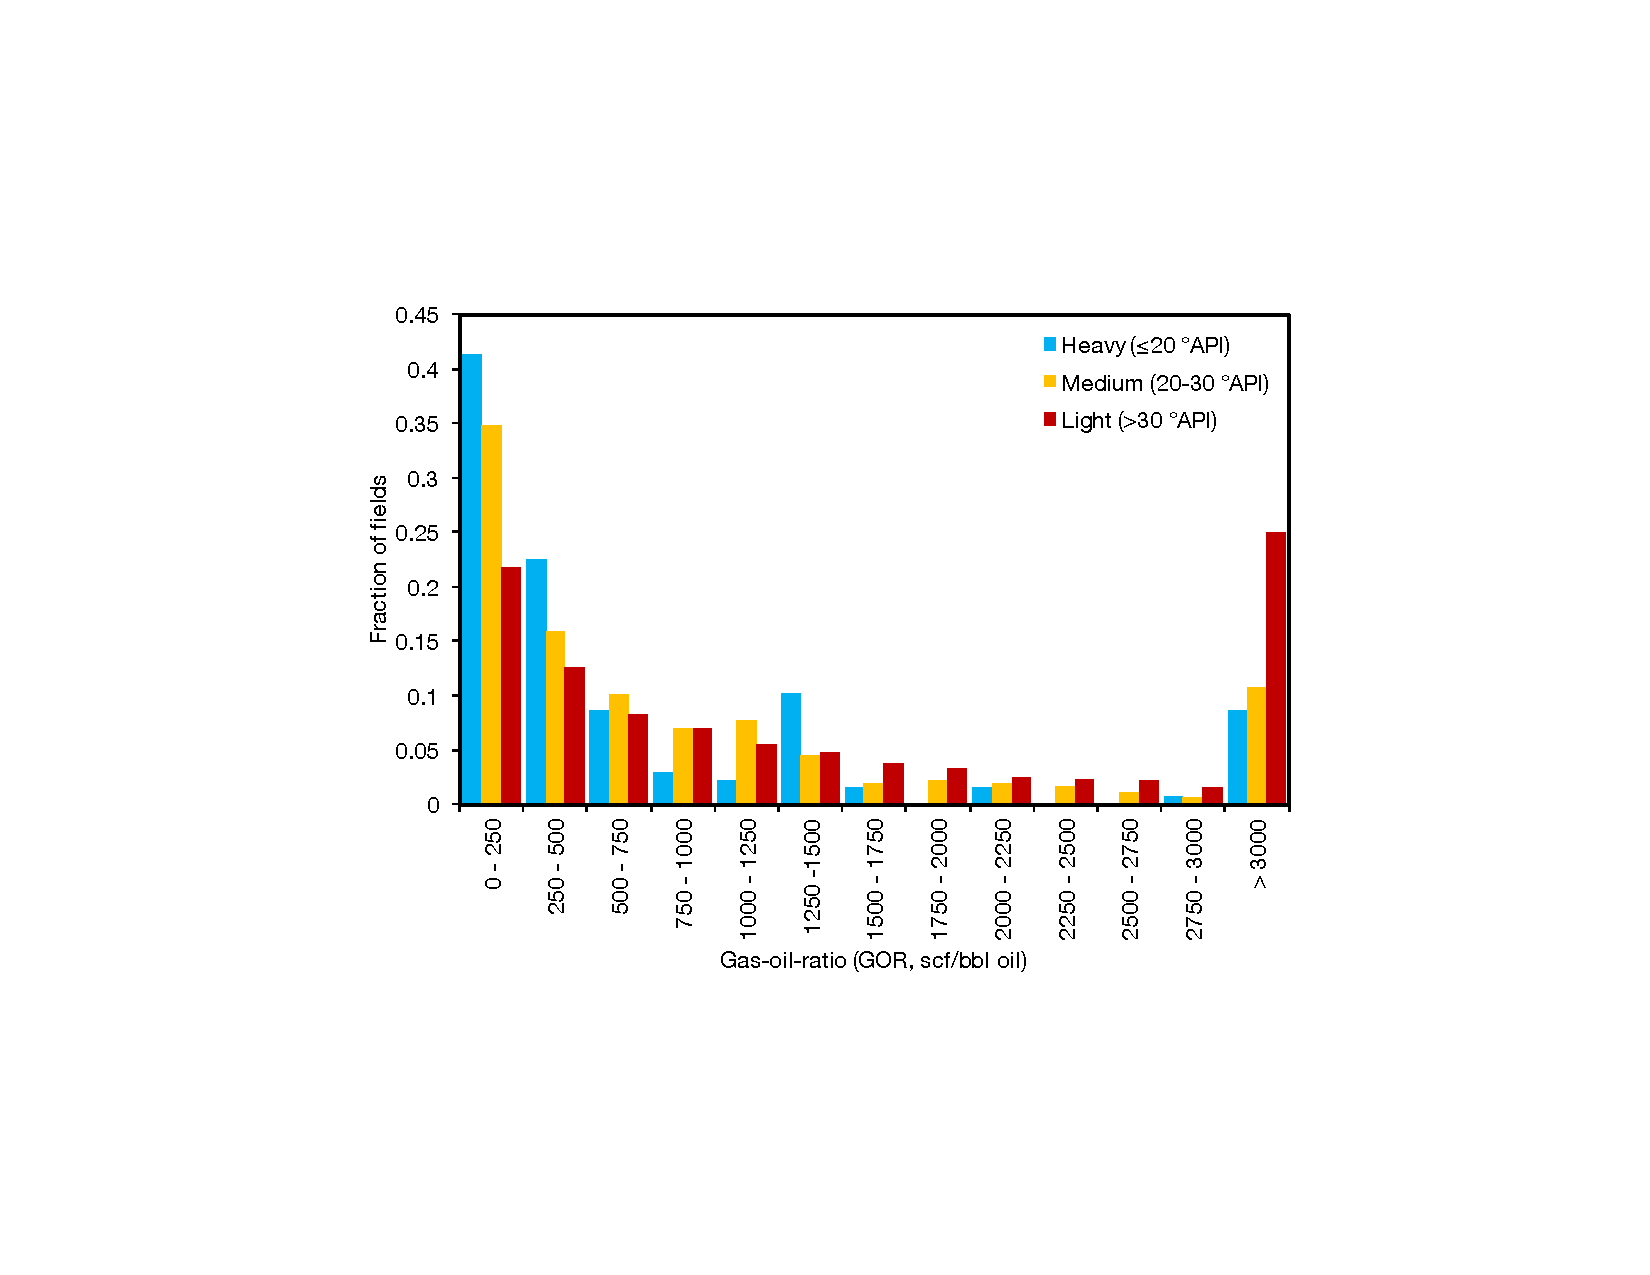
\includegraphics[width=0.8\columnwidth]{images/API-GOR.pdf}
\caption{Distributions of global GORs, binned by crude density.}
\label{fig:API-GOR}
\end{figure}

\begin{table}
\begin{scriptsize}
\caption{GOR values by crude oil API gravity bin.}
\label{tab:GOR_averages}
\begin{tabular*}{1\columnwidth}{p{0.15\columnwidth}p{0.08\columnwidth}p{0.15\columnwidth}p{0.15\columnwidth}p{0.1\columnwidth}p{0.1\columnwidth}p{0.1\columnwidth}}
\toprule
Crude bin & Num. fields & Gravity range & Avg. gravity & Mean GOR & Median GOR & SD GOR \\
& [\#] & [$^\circ$API] & [$^\circ$API] & [scf/bbl] & [scf/bbl] & [scf/bbl] \\
\midrule
Heavy & 149 & $<$ 20 & 16.4 & 1,122.4 & 333.3 & 2,829.7 \\
Medium & 758 & $\geq$ 20, $\leq$ 30 & 26.3 & 1,205.3 & 399.8 & 2,277.9 \\
Light & 2254 & $>$ 30 & 37.7 & 2,429.3 & 910.8 & 3,635.9 \\
\bottomrule
\end{tabular*}
\end{scriptsize}
\end{table}


\subsection{Default water oil ratio (WOR)} \label{WORSmartDefault}

Some defaults require more flexible (``smart'') default specifications. The water-oil-ratio (WOR, \xlname{WOR}) is a major parameter in influencing GHG emissions. OPGEE includes a statistical relationship for water production as a function of reservoir age. The default exponential relationship is a moderate case parameterized with a variety of industry data. Nevertheless, this relationship does not work well in predicting WOR for giant fields with very high per well productivity (e.g., Ghawar in Saudi Arabia).

A smart default for the water oil ratio as a function of field age was generated using data from large fields in various world regions. Data on oil and water production were extracted from reports issued by California Division of Oil, Gas and Geothermal Resources (DOGGR), Alberta Energy Resources Conservation Board (ERCB), Alaska Oil and Gas Conservation Commission (AOGCC), Natural Resources Canada (NRC), United Kingdom Department of Energy and Climate Change (DECC), and the Norwegian Petroleum Directorate (NPD). For the Norwegian fields, water production data were not available prior to the year 2000. For Alberta fields, data were not available prior to 1962. Only data for the first 60 years of production of a fields life were included. Only California fields contained data beyond 55 years, and therefore we excluded these years to avoid depleted field behavior in California from significantly affecting the least squares fit of a global relationship. 

Because the majority of crude oil that is marketed globally originates from larger oil fields, fields that have produced less than 100 million m$^3$ (630 million bbl) of crude oil were excluded. Also excluded from the analysis were fields that produce heavy crude using steam injection. 

Additionally, a small number of fields were excluded because of apparent data anomalies or unusual events that may have affected oil or water production. Both the Redwater field in Alberta and the Ninian field in UK North Sea were excluded for data anomalies. These fields have highly unusual water production data that can only be plausibly attributed to data entry error. Also, the Elk Hills field in California was excluded because it was part of the National Petroleum Reserve for many years and the Piper field in the UK was excluded because oil production was halted for several years. In total, data from 30 giant oil fields (12 onshore and 18 offshore) were included in the analysis. The largest and the only super-giant field to be included is Prudhoe Bay.


The default WOR is represented by an exponential function:

%%%%%%%%%%
\begin{minipage}{0.8\columnwidth}\label{eq:smart_default_WOR}
\begin{fleqn}[0pt]
\begin{equation}
WOR = a_{WOR} \exp [b_{WOR} ( t - t_0 )] - a_{WOR} \quad\quad\eqnunitfrac{bbl water}{bbl oil}
\end{equation}
\end{fleqn}
\end{minipage}\hfill
\begin{minipage}{0.3\columnwidth}
        \begin{tabular}{|cl}
        & \\
        $WOR$   & \xlname{WOR}\\
        & \\
\end{tabular}
\end{minipage}
%%%%%%%%%%
where $a_{WOR}$ = fitting constant for the initial $WOR$ in time = $t_0$ [bbl water/bbl oil]; $b_{WOR}$ = exponential growth rate [1/y]; $t_0$ = initial year of production (or year of discovery if year of first production unavailable) [y]; and $t$ = year being modeled (independent variable) [y]. Note that the pre-exponential $a_{WOR}$ is subtracted to force WOR to start at 0 when $t = t_0$. This model was fit to the collected data using a nonlinear least-squares fit from multiple starting points to ensure robustness of fit.

The results of fitting this model to the smart default fit values, compared to oil fields from a variety of world regions, is show in Figure \ref{fig:exponenital_fit_WOR}. The resulting fit gives $a_{WOR} = 4.020$ and $b_{WOR} = 0.024$. Figure \ref{fig:WOR_hist} histogram also shows that the 30 global oilfields WORs are distributed lognormally, with the majority of the data between 0-0.25 bbl water/bbl oil. 

The WOR data SDs are also plotted vs. field age, as shown in Figure \ref{fig:WOR_SD}. A power function with R$^2$ = 91\% is fitted to the data in order to be used as smart default WOR$_SD$:

%%%%%%%%%%
\begin{equation}\label{eq:smart_default_WOR_STDV}
WOR_{SD}(t) = C_{WOR}( t - t_0 )^{d_{WOR}} \quad\quad\eqnunitfrac{bbl water}{bbl oil}
\end{equation}
%%%%%%%%%%

Here \emph{C$_{WOR}$}=0.012 and \emph{d$_{WOR}$}=1.662. 

\begin{figure}
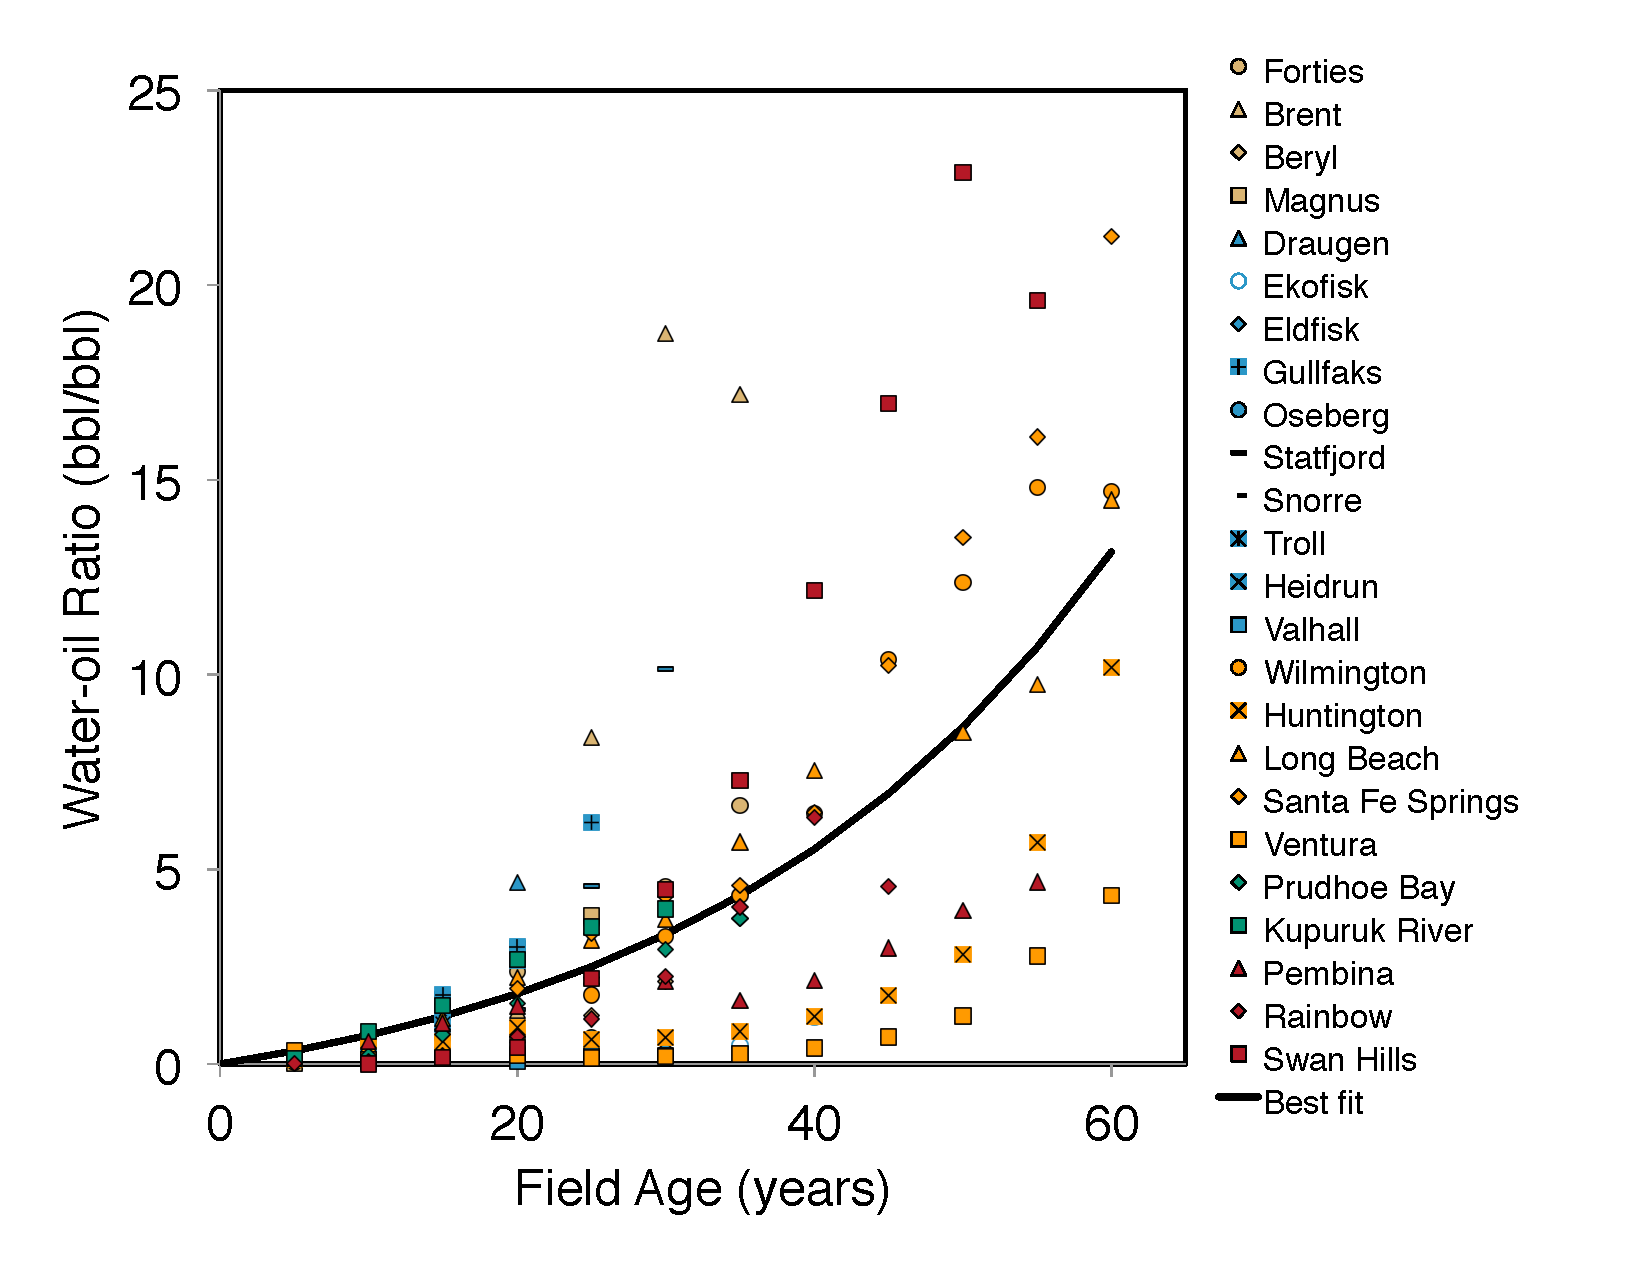
\includegraphics[width=1\columnwidth]{images/WOR_plot.pdf}
\caption{Exponential WOR model fit with smart default parameters. The best fit to data gives $a_{WOR} = 4.020$ and $b_{WOR} = 0.024$.}
\label{fig:exponenital_fit_WOR}
\end{figure}

\begin{figure}
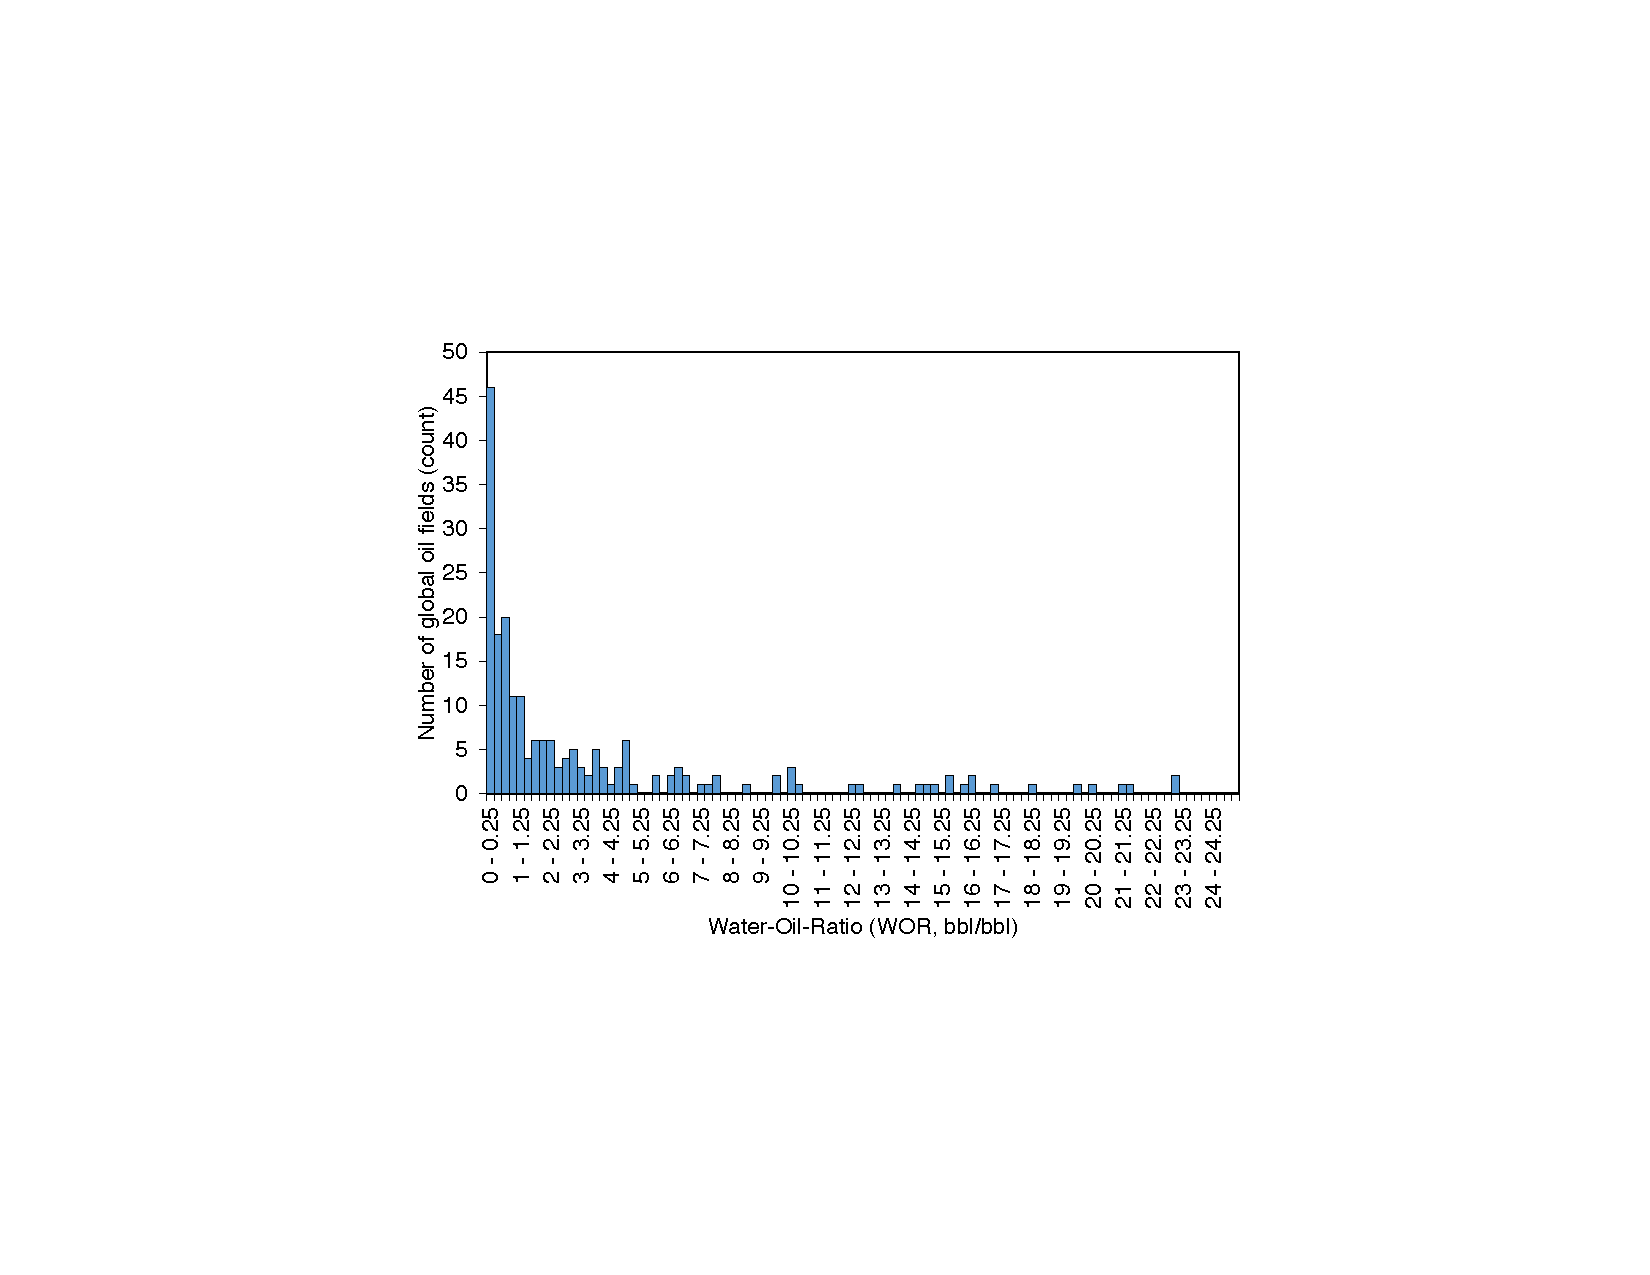
\includegraphics[width=1\columnwidth]{images/WOR_hist.pdf}
\caption{The WOR distribution of 30 global oilfields for bins of 0.25 bbl water/bbl oil.}
\label{fig:WOR_hist}
\end{figure}

\begin{figure}
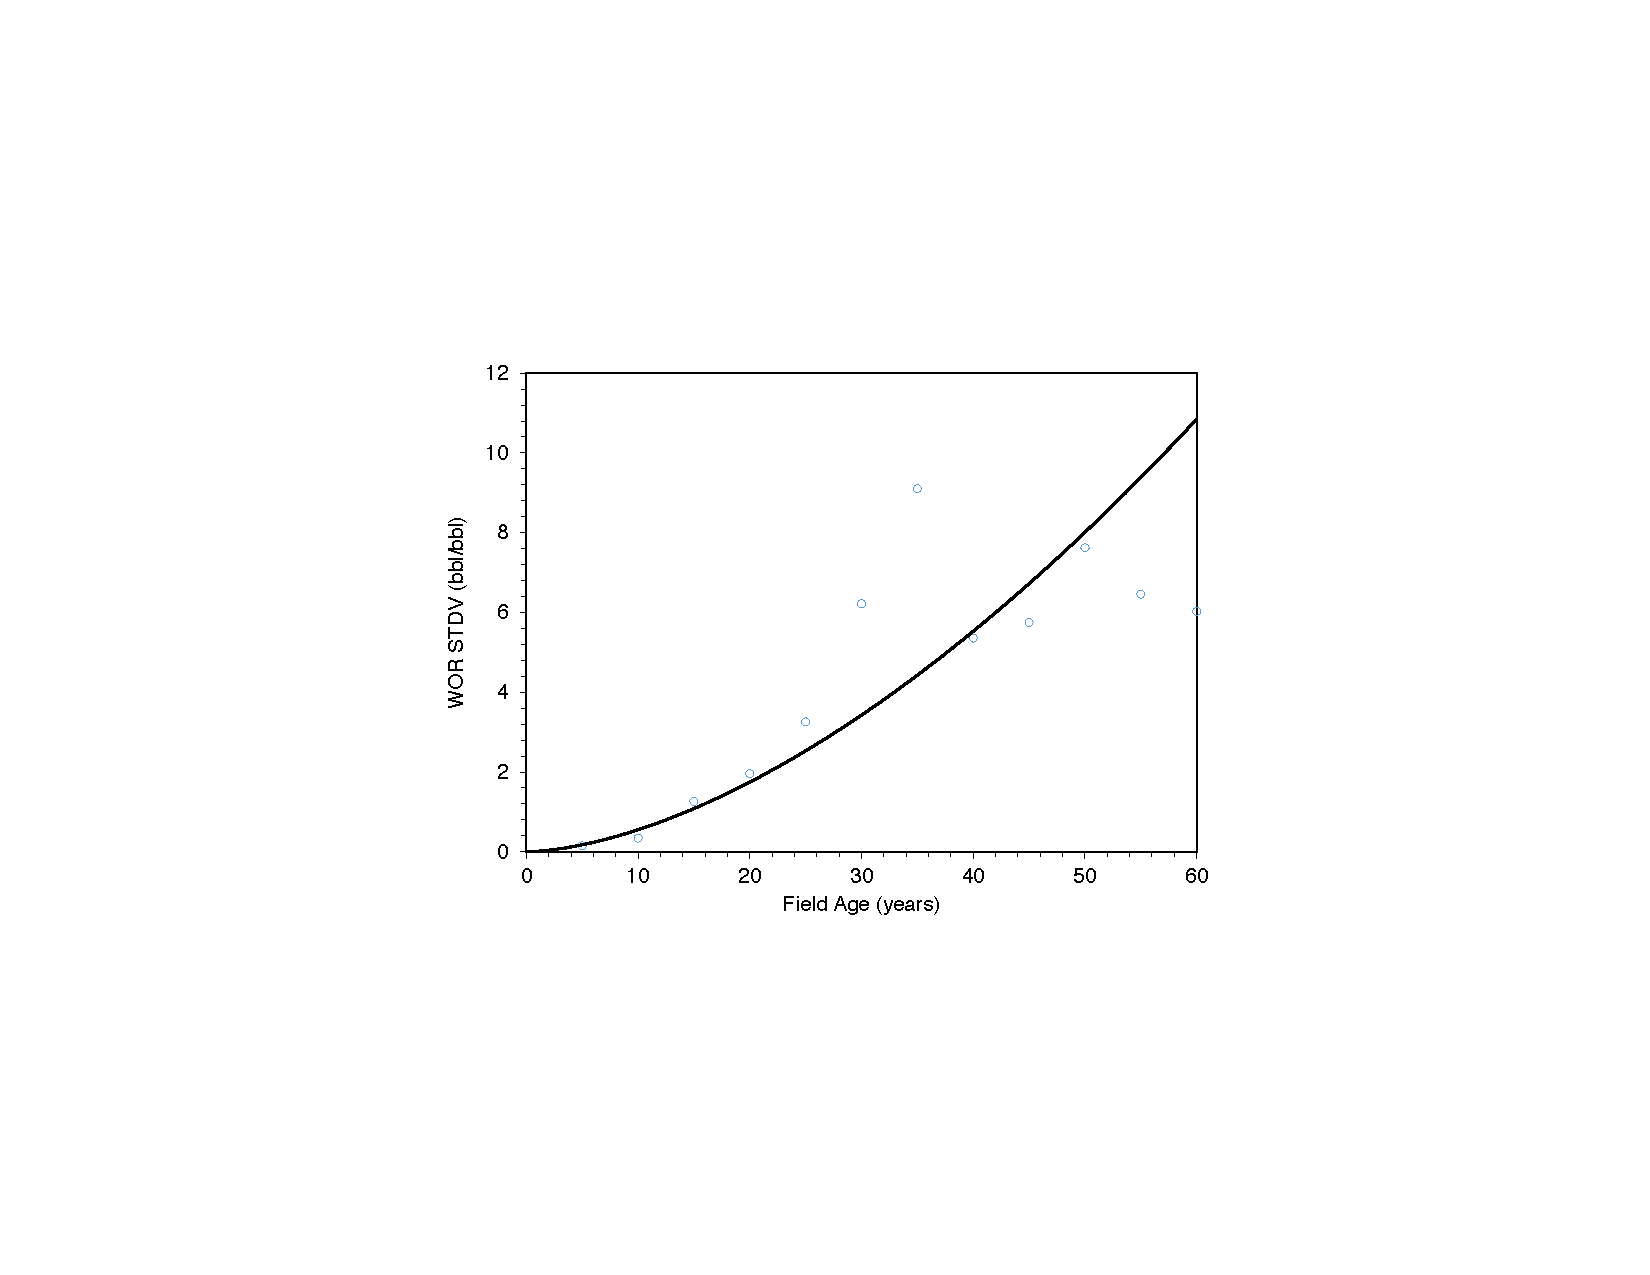
\includegraphics[width=1\columnwidth]{images/WOR_STDV.pdf}
\caption{Power WOR SD model fit with smart default parameters. }
\label{fig:WOR_SD}
\end{figure}


\subsection{Default waterflooding volume}

The volume of water injected in a waterflooding project (\xlname{WIR}) is meant to maintain reservoir pressure.As a default value, OPGEE assumes that the surface volume is replaced, such that the total oil produced plus the water produced is reinjected, or the injection per bbl = 1 + \xlname{WOR}.

\subsection{Default gas flooding injection ratio}

Gas flooding injection ratio (\xlname{GFIR}) is the ratio of the volume of flood gas injected [scf] to the volume of oil produced [bbl]. The volume of the oil is measured after bulk processing has removed the associated gas. The default flood gas injection ratio value depends on the choice of flood gas. If natural gas is selected as the flood gas, then the default ratio is calculated as follows:

%%%%%%%%%%
\begin{minipage}{0.6\columnwidth}\label{eq:NaturalGasAirOxygenFloodGasRatio}
\begin{fleqn}[0pt]
\begin{equation}
GFIR=1.5\cdot GOR \quad\quad\eqnunitfrac{scf gas}{bbl oil}
\end{equation}
\end{fleqn}
\end{minipage}\hfill
\begin{minipage}{0.3\columnwidth}
        \begin{tabular}{|cl}
        & \\
        $GFIR$   & \xlname{GFIR}\\
        $GOR$   & \xlname{GOR}\\
        & \\
        \end{tabular}
\end{minipage}

\begin{equation}
\end{equation}
%%%%%%%%%%
where $GFIR$ is gas flooding injection ratio [scf/bbl] and $GOR$ is the gas-oil-ratio [scf/bbl].

If N$_2$ is selected as the flood gas, then default $GFIR$ is 1,200 scf/bbl. This is based on the immiscible nitrogen flood operation at the Cantarell field in Mexico to maintain reservoir pressure. As described in the \nameref{sec:gas_flooding_compressor} section, the field operating equipment is designed to inject 1,200 mmscf/d \cite{Kuo2001}. In 2008, the injection rate was approximately 1,200 mmscf/d and the field was producing approximately 1.2 million bbl/d, leading to a default ratio of 1,200 scf/bbl \cite{Guzman2014}.

If CO$_2$ is selected as the flood gas, then default $GFIR$ is 10,000 scf/bbl. As with all injection ratios, $GFIR$ changes over the life cycle of the flood project. It can also vary based on the specific reservoir engineering strategies selected by the operator.  An example comes from DiPietro and Murrel (2013), who presented data from Kinder Morgan indicating that the injection ratio during the overall lifespan of an anonymous representative project was 6,000 scf/bbl. 

Another example is provided by Pyo et al. \cite{Pyo2003}, who reviewed the performance of a CO$_2$ flood at the Joffre Viking Pool in Alberta, Canada that had been active for approximately 30 years. The overall flood gas injection ratio during the life of the project was 10,800 scf/bbl; the ratios for the individual injector-producer well patterns within the field varied from 3,500 to 24,900 scf/bbl. 

The OPGEE default flood gas injection ratios are presented only as representative values that provide an order-of-magnitude estimate for when actual field data are not available. Actual field data should be obtained when possible.

\subsection{Default proportion of injected CO$_2$ that is recycled}
The OPGEE default for the proportion of CO$_2$ that breaks through to producing well is recycled (\xlname{Perc\_CO2\_breakthrough}) (not previously injected) is 59\%. This figure is from the Malone et al. \cite{NETL2014} discussion of an offshore CO$_2$ flood project at Weeks Island, Louisiana over an 9-year period (based on dates in the original reference by Johnston \cite{Johnson1988}). As with the flood gas injection ratio, actual data should be used if possible. 

\subsection{Default steam-oil-ratio (SOR)}

Because the SOR (\xlname{SOR}) is a key parameter driving GHG emissions from thermal oil production operations, we examine default values for SOR in more detail. 

SOR data are collected for California and Alberta thermal oil recovery operations for 2010 and 2011 \cite{DOGGR2010, DOGGR2011, DOGGRmonthly2010, ERCB2010, ERCB2011a}. 

For California operations, incremental SOR is calculated for 2009 using volumes of steam injected and reported incremental production due to steam injection. `Total' SOR is also calculated for 2009 using total production by field and total steam injection. For 2010, only monthly data are available, so incremental production data are not available. Therefore, only total SOR is reported.

For Alberta operations, data on bitumen produced and steam injected were collected for 24 thermal recovery projects (SAGD and CSS). No data were available on incremental rather than total production, and it is not clear what incremental production figures would represent bitumen operations where non-enhanced production would be very small.

Production volumes are binned by SOR for both regions and reported in Figure \ref{fig:SOR_dist}. Averages for SOR are presented in Table \ref{tab:SOR_stats}.  The default SOR in OPGEE \version \, is a conservative 3.0 bbl CWE per bbl oil. 

\begin{figure}[t]
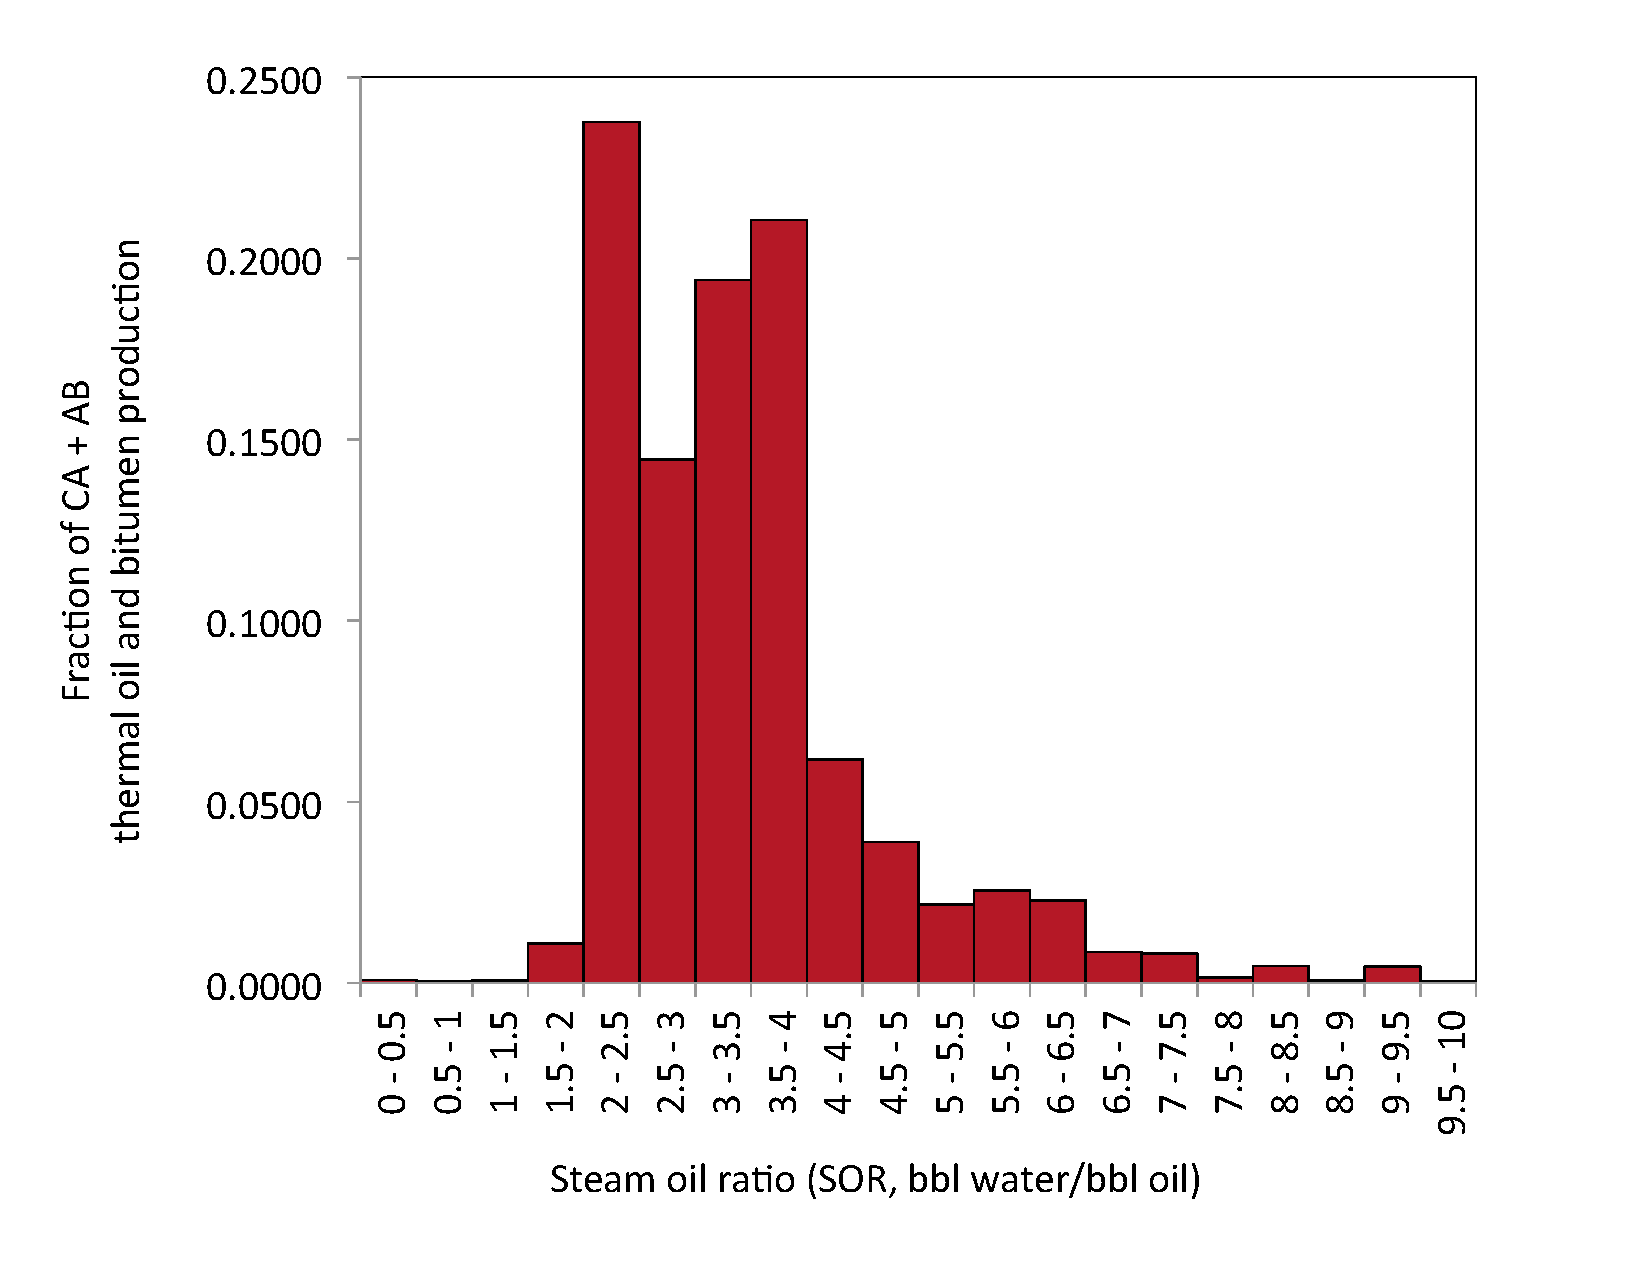
\includegraphics[width=0.85\columnwidth]{images/SOR_dist.pdf}
\caption{Distribution of SOR values for California and Alberta thermal EOR projects (steamflood, cyclic steam stimulation, steam-assisted gravity drainage).}
\label{fig:SOR_dist}
\end{figure}


\begin{table}
\caption{Indicators of SOR distributions for California and Alberta thermal EOR production. Units are bbl of cold water equivalent (CWE) per bbl of oil.}
\label{tab:SOR_stats}
\begin{scriptsize}
\begin{tabularx}{1\columnwidth}{p{0.3\columnwidth}p{0.15\columnwidth}p{0.15\columnwidth}}
\toprule
& Mean - SOR$_t$ & Mean - SOR$_i$ \\
\midrule
California - 2009 & 3.32 & 4.29 \\
California - 2010 & 3.41 & Unk. \\
Alberta - 2009 & 3.58 & NA \\
Alberta - 2010 & 3.32 & NA \\
\bottomrule
\end{tabularx}
\end{scriptsize}
\end{table}

\section{Probabilistic uncertainty analysis for missing key parameters}
\label{sec:Montecarlo}

As mentioned before, OPGEE uses approximately 50 primary input parameters as input data for each field in order to perform an assessment. If input data are not available for some of these parameters (common due to lack of publicly available data), OPGEE uses smart defaults (see Section \ref{sec:smart_defaults}) to fill missing information (deterministic analysis). What if one does not want to use OPGEE defaults? Then what is the uncertainty associated with using defaults in place of the missing data?

It has been shown before that emissions uncertainty depends on the key input parameters, and the use of default values in the place of specific data (\cite{brandt2014uncertainty,vafi2014uncertainty}). Therefore, OPGEE only analyzes the uncertainty associated with missing input parameters in \sheet{Inputs} worksheet. Other uncertainty sources include: unchanging parameters embedded into OPGEE (e.g. downhole pump efficiency, etc.), model structure, and modeling equations used for process units.

In OPGEE 3.0, the uncertainty associated with the GHG emissions estimates can be computed probabilistically using a Monte Carlo (MC) simulation method. In each Monte Carlo realization, for each field, missing data are replaced not with the OPGEE default value but instead with a value from the underlying distribution or statistical values presented in Section \ref{sec:smart_defaults}. Also, venting and fugitive emissions are drawn from empirical observations rather than using averages. The total number of Monte Carlo realizations per field can be determined by the user at the top panel of \sheet{Inputs} worksheet. It should be pointed out that the convergence analysis shows that after about 300 realizations, a consistent result distribution can be obtained per field. This implies that more MC simulations no longer strongly affects mean, median or standard deviation (SD) of uncertainty realizations. 

A summary of input parameters and their probabilistic distribution indices used for this analysis are listed in Table \ref{tab:Montecarlo}. The same indices are included from columns \emph{M} to \emph{U} of \sheet{Active Field} sheet where the user can customize the uncertainty analysis assumptions and settings. See \cite{Masnadi2018} for an example of global oilfields GHG emissions uncertainty analysis using OPGEE.

\begin{landscape}
\begin{scriptsize}
\tablefirsthead{\toprule Input Parameters {[}unit{]} & Mean     & SD       & Low Range & High Range & Prob. Yes (binary) & Distribution Type \\
\midrule}
\tablehead{ \multicolumn{8}{p{1\columnwidth}}{\textit{Continued from previous page}}\\ \toprule Input Parameters {[}unit{]} & Mean     & SD       & Low Range & High Range & Prob. Yes (binary) & Distribution Type \\
\midrule }
\tabletail{\bottomrule \multicolumn{8}{p{1\columnwidth}}{\textit{Continued on next page...}}\\}
\tablelasttail{\bottomrule}
\tablecaption{Summary of input default parameters and their probabilistic distribution measure used in \sheet{Active Field} worksheets.}
\label{tab:Montecarlo}
\begin{supertabular*}{1\columnwidth}{p{0.4\columnwidth}p{0.09\columnwidth}p{0.05\columnwidth}p{0.05\columnwidth}p{0.05\columnwidth}p{0.05\columnwidth}p{0.05\columnwidth}p{0.1\columnwidth}}
\midrule
Production methods &            &           &            &                    &                   \\                                                              \midrule
Downhole pump \xlname{Downhole\_Pump\_01}                                                                                                                                            & 0        & 0          & 0         & 0          & 0.95               & Binary            \\
Water reinjection \xlname{Water\_reinjection\_01}                                                                                                                                       & 0        & 0          & 0         & 0          & 0.25               & Binary            \\
Natural gas reinjection \xlname{Natural\_gas\_reinjection\_01}                                                                                                                                  & 0        & 0          & 0         & 0          & 0.95               & Binary            \\
Water flooding \xlname{Water\_flooding\_01}                                                                                                                                           & 0        & 0          & 0         & 0          & 0.75               & Binary            \\
Gas lifting \xlname{Gas\_lifting\_01}                                                                                                                                           & 0        & 0          & 0         & 0          & 0.05               & Binary            \\
Gas flooding \xlname{Gas\_flooding\_01}                                                                                                                                     & 0        & 0          & 0         & 0          & 0.05               & Binary            \\
Steam flooding \xlname{Steam\_flooding\_01}                                                                                                                                           & 0        & 0          & 0         & 0          & 0                  & Binary            \\
 Oil sands mine \xlname{Oil\_sands\_mine\_int\_01}                                                                                                                                          & 0        & 0          & 0         & 0          & 0                  & Binary            \\
Oil sands mine \xlname{Oil\_sands\_mine\_nonint\_01}                                                                                                                                     & 0        & 0          & 0         & 0          & 0                  & Binary            \\
\midrule
Field properties                                                                                                                                            &          &            &           &            &                    &                   \\
\midrule
Field age \xlname{Field\_age} \emph{t}) {[}y{]}                                                                                                                                    & 38       & 22         & 2         & 82         & -                  & Lognormal         \\
 Field depth \xlname{Field\_depth} {[}ft{]}                                                                                                                              & 7,122    & 3,851      & 59        & 35,837     & -                  & Lognormal         \\
Oil production volume \xlname{Oil\_prod} {[}bbl/d{]}                                                                                                                  & 2,098    & 2,445      & 10        & 10,000     & -                  & Lognormal         \\
Number of producing wells \xlname{Num\_prod\_wells} {[}\#{]}                                                                                                                       & \xlname{Oil\_prod}/87.5 & 2,445/87.5 & 1         & 114        & -                  & Lognormal         \\
Number of water injecting wells \xlname{Num\_water\_inj\_wells} {[}\#{]}                                                                                                                 & Tab. \ref{tab:inj_prod_ratios} & Tab. \ref{tab:inj_prod_ratios}   & 1         & 95         & -                  & Lognormal         \\
Well diameter \xlname{Well\_diam} {[}inch{]}                                                                                                                                 & 3        & 1          & 1         & 5          & -                  & Triangular        \\
Productivity index \xlname{Prod\_index} {[}bbl/psi-d{]}                                                                                                                  & 17       & 18         & 1         & 50         & -                  & Lognormal         \\
Average reservoir pressure \xlname{Res\_press} {[}psi{]}                                                                                                              &  eq. \ref{eq:res_pressure1}   & eq. \ref{eq:res_pressure1}     & 24        & 14,738     & -                  & Lognormal         \\
Average reservoir temperature \xlname{Res\_temp} {[}$^{\circ}$F{]}                                                                                                            & eq. \ref{eq:res_temp}  & eq. \ref{eq:res_temp}      & 71        & 582        & -                  & Normal            \\
Offshore? \xlname{Offshore\_01}                                                                                                                                                 & 0        & 0          & 0         & 0          & 0.2                & Binary            \\
\midrule
3. Fluid properties                                                                                                                                            &          &            &           &            &                    &                   \\
\midrule
API gravity of produced crude \xlname{API\_grav} {[}$^{\circ}$API{]}                                                                                                                 & 33       & 8          & 3         & 88         & -                  & Normal            \\
Associated gas composition {[}mol\%{]}                                                                                                                   &          &            &           &            &                    &                   \\
N$_2$ \xlname{Gas\_comp\_N2}                                                                                                                                                             & Tab. \ref{tab:gas_composition}        & -          &1         & 8         & -                  & Lognormal         \\
CO$_2$ \xlname{Gas\_comp\_CO2}                                                                                                                                                                       & Tab. \ref{tab:gas_composition}         & -          & 0         & 2         & -                  & Lognormal         \\
C$_1$ \xlname{Gas\_comp\_C1}                                                                                                                                                                      & Tab. \ref{tab:gas_composition}        & -          & 79       & 96        & -                  & Lognormal         \\
C$_2$ \xlname{Gas\_comp\_C2}                                                                                                                                                                       & Tab. \ref{tab:gas_composition}         & -          & 2         & 11         & -                  & Lognormal         \\
C$_3$ \xlname{Gas\_comp\_C3}                                                                                                                                                                     & Tab. \ref{tab:gas_composition}         & -          & 0         & 4         & -                  & Lognormal         \\
C$_4$+ \xlname{Gas\_comp\_C4}                                                                                                                                                                    & Tab. \ref{tab:gas_composition}         & -          & 0         & 2          & -                  & Lognormal         \\
H$_2$S \xlname{Gas\_comp\_H2S}                                                                                                                                                                      & Tab. \ref{tab:gas_composition}       & -          & 0         & 0.05          & -                  & Lognormal         \\
\midrule
Production practices                                                                                                                                        &          &            &           &            &                    &                   \\
\midrule
Gas-to-oil ratio \xlname{GOR} {[}scf/bbl oil{]}                                                                                                                 & Tab. \ref{tab:GOR_averages} & Tab. \ref{tab:GOR_averages}   & 1         & 34,000     & -                  & Lognormal         \\
Water-to-oil ratio \xlname{WOR} {[}bbl produced/bbl oil{]}                                                                                                      & eq. \ref{eq:smart_default_WOR}   & eq. \ref{eq:smart_default_WOR}     & 1         & 33         & -                  & Lognormal         \\
 Water injection ratio \xlname{WIR}  {[}bbl injected/bbl oil{]}                                                                                                         & \xlname{WOR}+1    & 0          & \xlname{WOR}+1     & \xlname{WOR}+1      & -                  & Uniform           \\
Gas lifting injection ratio \xlname{GLIR} {[}scf/bbl oil{]}                                                                                                            & 363      & 500        & 200       & 2500       & -                  & Lognormal         \\
Gas flooding injection ratio \xlname{GFIR} {[}scf/bbl oil{]}                                                                                                           & eq. \ref{eq:NaturalGasAirOxygenFloodGasRatio}   & 0          & eq. \ref{eq:NaturalGasAirOxygenFloodGasRatio}    & eq. \ref{eq:NaturalGasAirOxygenFloodGasRatio}     & -                  & Uniform           \\
Flood gas (1:Natural gas, 2: N$_2$, 3: CO$_2$) \xlname{Flood\_gas\_type}                                                                                                               & 1        & 0          & 1         & 1          & -                  & Uniform           \\
CO$_2$ flooding and sequestration parameters                                                                                                                &          &            &           &            &                    &                   \\
Fraction of CO$_2$ breaking through \xlname{Perc\_CO2\_breakthrough}                                                                   & 41       & 20         & 0         & 100        & -                  & Normal            \\
Source of CO$_2$ \xlname{Source\_CO2} (1: Natural subsurface reservoir, 2: Anthropogenic)                                                                                      & 1        & 0          & 1         & 1          & -                  & Uniform           \\
Percentage of sequestration credit assigned to the oilfield \xlname{Perc\_sequestration\_credit}                                                                                            & 0        & 0          & 0         & 0          & -                  & Uniform           \\
Steam-to-oil ratio \xlname{SOR} {[}bbl steam/bbl oil{]}                                                                                                         & 3.5      & 2          & 0         & 5          & -                  & Lognormal         \\
Fraction of required electricity generated onsite \xlname{Fraction\_elec\_onsite}                                                                                                        & 0.5      & 0.25       & 0         & 1          & -                  & Normal            \\
 Fraction of remaining gas reinjected \xlname{Fraction\_remaining\_gas\_inj}                                                                                                                      & 0.5      & 0.25       & 0         & 1          & -                  & Normal            \\
Fraction of water produced that is reinjected \xlname{Fraction\_water\_reinjected}                                                                                                             & 0.77     & 0.38       & 0         & 1          & -                  & Normal            \\
Fraction of steam generation via co-generation \xlname{Fraction\_steam\_cogen}                                                                                                           & 0.37     & 0.42       & 0         & 1          & -                  & Normal            \\
\midrule
Processing practices                                                                                                                                        &          &            &           &            &                    &                   \\
\midrule
 Heater/treater \xlname{Heater\_treater}                                                                                                                                           & 0        & 0          & 0         & 0          &                    & Binary            \\
Stabilizer column \xlname{Stabilizer}                                                                                                                                        & 0        & 0          & 0         & 0          &                    & Binary            \\
Upgrader type \xlname{Upgrader\_type} (0: None, 1: Delayed coking, 2: Hydroconversion, 3: Hydroconversion and fluid coking)                                                      & 0        & 0          & 0         & 0          & 0                  & Uniform           \\
Associated gas processing path \xlname{Gas\_processing\_path} (1: None, 2: Minimal - Dehydrator, 3: Acid Gas, 4: Wet Gas, 5: Acid Wet Gas, 6: CO$_2$-EOR Membrane, 7: CO$_2$-EOR Ryan Holmes) & 5        & 0          & 5         & 5          & -                  & Uniform           \\
 Flare-oil-ratio \xlname{FOR} {[}scf flared/bbl oil{]}                                                                                                           & NOAA     & NOAA*0.2   & 1         & 3000       & -                  & Normal            \\
 Ratio of venting to oil production \xlname{VOR}                                                                                                                       & 10       & 3          & 0         & 100        & -                  & Normal            \\
Volume fraction of diluent in diluted crude \xlname{Fraction\_diluent}                                                                                                             & 0        & 0          & 0         & 0          & -                  & Uniform           \\
\midrule
 Land use impacts                                                                                                                                            &          &            &           &            &                    &                   \\
\midrule
Crude ecosystem carbon richness                                                                                                                          &          &            &           &            &                    &                   \\
Low carbon richness (semi-arid grasslands) \xlname{Low\_ecosystem\_richness\_01}                                                                                                             & 0        & 0          & 0         & 0          & 0.33               & Binary            \\
Moderate carbon richness (mixed) \xlname{Med\_ecosystem\_richness\_01}                                                                                                                        & 0        & 0          & 0         & 0          & 0.33               & Binary            \\
 High carbon richness (forested) \xlname{High\_ecosystem\_richness\_01}                                                                                                                         & 0        & 0          & 0         & 0          & 0.33               & Binary            \\
Field development intensity                                                                                                                              &          &            &           &            &                    &                   \\
Low intensity dev. and low oxidation \xlname{Low\_land\_disturbance\_01}                                                                                                                   & 0        & 0          & 0         & 0          & 0.33               & Binary            \\
Moderate intensity dev. and moderate oxidation \xlname{Med\_land\_disturbance\_01}                                                                                                          & 0        & 0          & 0         & 0          & 0.33               & Binary            \\
High intensity dev. and high oxidation \xlname{High\_land\_disturbance\_01}                                                                                                                  & 0        & 0          & 0         & 0          & 0.33               & Binary            \\
\midrule
Crude oil transport                                                                                                                                         &          &            &           &            &                    &                   \\
\midrule
Fraction of oil transported by each mode                                                                                                                 Ocean tanker \xlname{Fraction\_oil\_transport\_tanker}                                                                                                                                           & 0        & 0          & 0         & 0          & 1                  & Binary            \\
Barge \xlname{Fraction\_oil\_transport\_barge}                                                                                                                                                   & 0        & 0          & 0         & 0          & 0                  & Binary            \\
Pipeline \xlname{Fraction\_oil\_transport\_pipeline}                                                                                                                                                & 0        & 0          & 0         & 0          & 1                  & Binary            \\
Rail \xlname{Fraction\_oil\_transport\_rail}                                                                                                                                                    & 0        & 0          & 0         & 0          & 0                  & Binary            \\
Truck \xlname{Fraction\_oil\_transport\_truck}                                                                                                                                                  & 0        & 0          & 0         & 0          & 0                  & Binary            \\
Transport distance (one way)                                                                                                                             &          &            &           &            &                    &                   \\
Ocean tanker \xlname{Oil\_transport\_distance\_tanker} {[}mile{]}                                                                                                                                & 8,000    & 2,000      & 1,000     & 12,000     & -                  & Normal            \\
Barge \xlname{Oil\_transport\_distance\_barge} {[}mile{]}                                                                                                                                       & NA       & NA         & NA        & NA         & -                  & NA                \\
Pipeline \xlname{Oil\_transport\_distance\_pipeline} {[}mile{]}                                                                                                                                    & 1,000    & 700        & 100       & 5,000      & -                  & Normal            \\
Rail \xlname{Oil\_transport\_distance\_rail} {[}mile{]}                                                                                                                                        & NA       & NA         & NA        & NA         & -                  & NA                \\
Truck \xlname{Oil\_transport\_distance\_truck} {[}mile{]}                                                                                                                                        & NA       & NA         & NA        & NA         & -                  & NA                \\
Ocean tanker size, if applicable \xlname{Ocean\_tanker\_size} {[}ton{]}                                                                                                               & 250,000  & 25,000     & 50,000    & 300,000    & -                  & Normal            \\
\midrule
Other sources emissions                                                                                                                                    &          &            &           &            &                    &                   \\
\midrule
Small sources emissions \xlname{Small\_sources\_adder}   {[}g CO$_2$eq/MJ{]}                                                                                                                & 0.5      & 0.15       & 0.1       & 1          & -                  & Normal \\
\end{supertabular*}
\end{scriptsize}
\end{landscape}

 
         

%%%%%%%%%%%%%%%%%%%%%%%%%%%%%%%%%%%%%%%%%%%%%
%%%%%%%%%%%%%%%%%%%%%%%%%%%%%%%%%%%%%%%%%%%%%
%%%%%%%%%%%%%%%%%%%%%%%%%%%%%%%%%%%%%%%%%%%%%

\chapter{Flow sheet}

%%%%%%%%%%%%%%%%%%%%%%%%%%%%%%%%%%%%%
\section{Flow sheet introduction}\label{sec:gas_balance}

The flow sheet is the main organizing sheet for tying OPGEE process modules together and tracking the flow of fluids through the system. It includes graphical representation of the process flows and numerical results for all streams. 

\section{Flow table}

At the top of the \sheet{Flow sheet} is the \xlname{FlowTable} (see Figure \ref{fig:FlowSheet}). In the \xlname{FlowTable} Streams are numbered 1-300 (with gaps for forward compatibility and model extension). At the top of the table, each stream can contain mass flow of a given set of tracked substances.  In the lower section of the flow table, a variety of other characteristics of each stream are computed. These properties are computed for all streams using equivalent formulas.

\begin{figure}[!h]
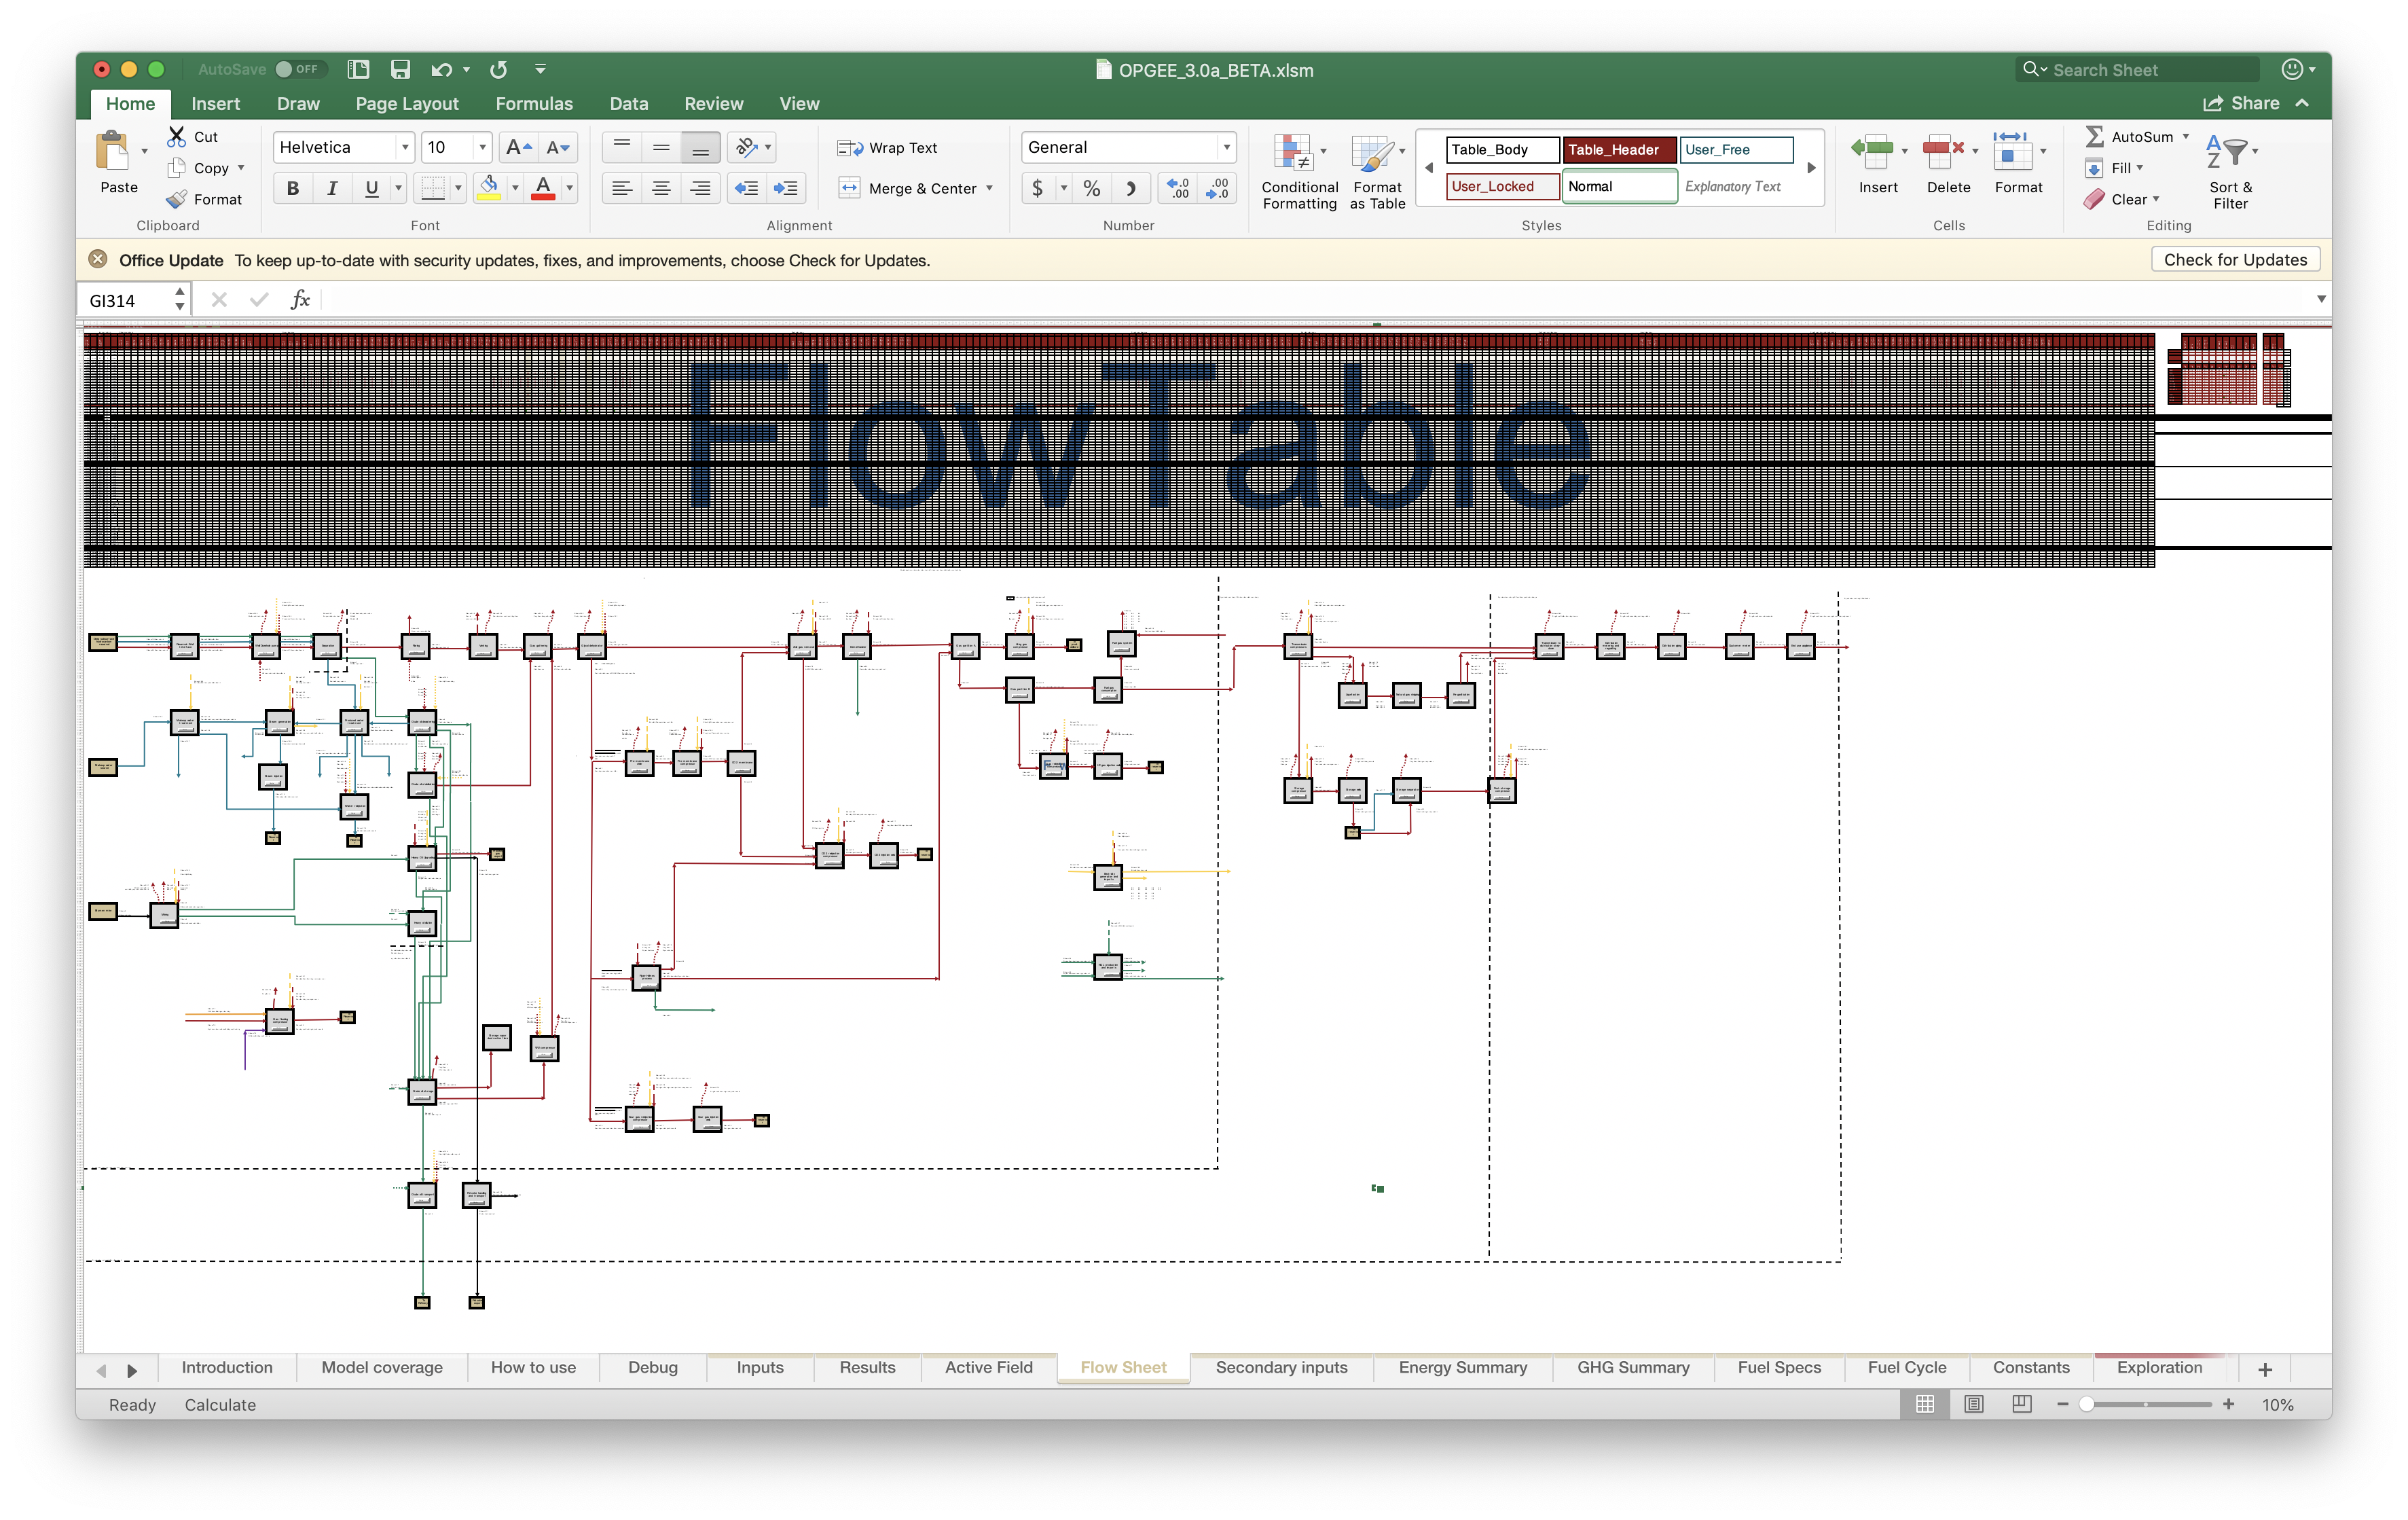
\includegraphics[width=0.70\columnwidth]{images/FlowSheet.png}
\caption{Flow sheet at maximum dimension showing the flow table at top and the process flow diagram below.}
\label{fig:FlowSheet}
\end{figure}

To look up a given stream property, the ``Index'' function in Excel is used. The syntax of the Index function is as follows:
\begin{verbatim}
Index([Table],[Row],[Column])
\end{verbatim}
where \verb+[Table]+ is the name of the table being accessed, and \verb+[Row]+ and \verb+[Column]+ are the row and column of the entry desired.

In order to call a quantity from the Flow table, the proper syntax would then be:
\begin{verbatim}
Index(FlowTable,PROP_NAME,STREAM_NUM)
\end{verbatim}
where \verb+PROP_NAME+ is the name of the property desired and \verb+STREAM_NUM+ is the number of the stream of interest.

The property names are defined below.

\section{Computing properties of flows}

\subsection{Mass flows}

Mass flows per day are named \xlname{M\_X} where \xlname{X} is a place holder for a given stream component [tonne/d].  The following streams are recognized in OPGEE:
\begin{itemize}
\item \xlname{PC} -- Petroleum coke streams
\item  \xlname{O} -- Oil streams
\item  \xlname{LPG} -- Liquified petroleum gas streams
\item \xlname{W} -- Water stream
\item  \xlname{N2} -- Nitrogen stream
\item  \xlname{O2} -- Oxygen stream
\item  \xlname{CO2} -- Carbon dioxide stream
\item  \xlname{H2O} -- Water vapor stream
\item  \xlname{C1} -- Methane stream
\item  \xlname{C2} -- Ethane stream
\item  \xlname{C3} -- Propane stream
\item  \xlname{C4} -- Butane stream
\item  \xlname{CO} -- Carbon monoxide stream
\item  \xlname{H2} -- Hydrogen stream
\item  \xlname{H2S} -- Hydrogen sulfide stream
\item \xlname{SO2} -- Sulfur dioxide stream
\end{itemize}

The only solid component tracked in the \sheet{Flow sheet} is petroleum coke \xlname{PC}. Petroleum coke is a solid form of primarily carbon, generated at crude oil upgrading and refining facilities. 

Three liquid components are tracked in the \sheet{Flow sheet}.  Oil streams \xlname{O} are defined as hydrocarbon streams that are liquid at standard temperature and pressure. For simplicity, bitumen is considered a liquid oil stream. Oil streams vary from API gravity of 6 $^\circ$API (heavy bitumen) to 70 $^\circ$API (light condensate or diluent). Liquified petroleum gas (LPG) streams \xlname{LPG} are gaseous at ambient temperature and pressure but will liquefy at low pressure and therefore are commonly transported in dense form (commonly: propane and butane). Water \xlname{W} can represent either brackish or fresh water.

Twelve gas components are tracked in the \sheet{Flow sheet}. These include constituents of air (\xlname{N2}, \xlname{O2}, \xlname{CO2}, and \xlname{H2O}). Note that water vapor is represented by \xlname{H2O} while liquid phase water is tracked as \xlname{W}.  Next are the four light hydrocarbons, \xlname{C1} - \xlname{C4}. Some sources distinguish a species in gas called ``pentanes plus''. Given that these are liquid at standard temperature and pressure, these would be considered a very light oil stream. Similarly, lease condensate and natural gas plant liquids are also tracked as oil \xlname{O} and not treated separately. Lastly, minor constituents are tracked: \xlname{CO}, \xlname{H2}, \xlname{H2S}, and \xlname{SO2}.


\subsection{Electricity flows}

Electricity is tracked by its energy flow rate per day [MWh/d] \xlname{E\_EL}. No distinction is made between high voltage or low voltage electricity, nor do we distinguish between DC and AC power.

\subsection{Properties of phases}

Certain properties are tracked for the composite of all phases in the stream.  These include temperature [$^\circ$F] \xlname{T}, absolute temperature  [$^\circ$R], \xlname{T\_ABS}, pressure [psia] \xlname{P}. We ignore pressure differences due to phase boundaries (i.e., arising due to surface tension) and therefore assume that all species present in a single stream are present at the same pressure.

Each stream is also classified using 0-1 binary parameters as containing oil \xlname{OIL\_01}, containing liquid phase water \xlname{WAT\_01}, and containing gases \xlname{GAS\_01}. These 0-1 binary parameters are used in logical flows for computing properties of different streams.

\subsection{Properties of oil}
\label{sec:oil_properties}

A number of properties of oil are tracked.  These properties can be a function of oil chemistry (e.g., heating value) as well as the temperature and pressure of the oil stream (e.g., solution gas oil ratio).

\paragraph{API gravity of oil}


The API gravity of the oil is tracked as variable in the flow sheet \xlname{API\_O}.  For conventional oil streams, this is generally defined as equal to the defined input parameter \xlname{API\_grav} (streams given in Table \ref{tab:Source_API_Gravity}).  For bitumen streams it is equal to defined input parameter \xlname{Bitumen\_API}.  For diluent streams it is equal to \xlname{Diluent\_API}. For LPG the API gravity is not computed as this parameter is not typically used to represent these products.

\begin{table}
\begin{scriptsize}
\caption{Source of API gravity for oil streams.}
\label{tab:Source_API_Gravity}
\begin{tabularx}{1\columnwidth}{p{0.05\columnwidth}p{0.35\columnwidth}p{0.2\columnwidth}p{0.1\columnwidth}p{0.1\columnwidth}}
\toprule
Stream num. & Stream name	&	Source of API gravity term		& Default		& Notes \\
\midrule
\stream{1}		& Crude oil in reservoir	& \xlname{API\_grav}			& 30$^\circ$ API &  \\
\stream{2}		& Bitumen in mine		& \xlname{API\_Bitumen}				& 30$^\circ$ API &  \\
\stream{3}		& Crude oil at well bottom	& \xlname{API\_grav}			& 30$^\circ$ API &  \\
\stream{4}		& Crude oil at wellhead	& \xlname{API\_grav}				& 30$^\circ$ API &  \\
\stream{5}		& Bitumen from mine to upgrader	& \xlname{API\_Bitumen}		& 30$^\circ$ API &  \\
\stream{6}		& Bitumen from mine to dilution	& \xlname{API\_Bitumen}		& 30$^\circ$ API &  \\
\stream{7}		& Crude oil after separator	& \xlname{API\_grav}			& 30$^\circ$ API &  \\
\stream{8}		& Crude oil to stabilizer	& \xlname{API\_grav}			& 30$^\circ$ API &  \\
\stream{9}		& Crude oil to storage	& \xlname{API\_grav}				& 30$^\circ$ API &  \\
\stream{10}		& Stabilized crude to storage	& \xlname{API\_grav}		& 30$^\circ$ API &  \\
\stream{11}		& Upgraded crude to storage	& \xlname{API\_grav}			& 30$^\circ$ API &  \\
\stream{12}		& Diluted bitumen to storage	& \xlname{API\_grav}		& 30$^\circ$ API &  \\
\stream{13}		& Crude oil to transport	& \xlname{API\_grav}			& 30$^\circ$ API &  \\
\stream{14}		& Transported crude oil at refinery	& \xlname{API\_grav}    & 30$^\circ$ API &  \\
\stream{15}		& Petcoke export from upgrader	& -				& NA &  \\
\stream{16}		& NGL/diluent to dilution	& \xlname{API\_diluent}			& 30$^\circ$ API &  \\
\stream{17}		& LPG to blend with crude oil	& \xlname{API\_diluent}		& 30$^\circ$ API &  \\
\stream{18}		& LPG to direct sales	& \xlname{API\_diluent}				& 30$^\circ$ API &  \\
\stream{19}		& Crude oil to upgrader	& \xlname{API\_grav}				& 30$^\circ$ API &  \\
\stream{20}		& Crude oil in dilution	& \xlname{API\_grav}				& 30$^\circ$ API &  \\
\bottomrule
\end{tabularx}
\end{scriptsize}
\end{table}

\paragraph{Specific gravity of oil}

The specific gravity of the oil is tracked as variable \xlname{GAMMA\_O}. Specific gravity is the density of a fluid compared to the density of water, both measured at 60 $^\circ$F and atmospheric pressure. Specific gravity is computed from the API gravity as follows:

\begin{minipage}{0.6\columnwidth}
\begin{fleqn}[0pt]
\begin{equation}
\gamma_o = \frac{141.5}{131.5 + API} \eqnunitfrac{g}{g}
\end{equation}
\end{fleqn}
\end{minipage}\hfill
\begin{minipage}{0.3\columnwidth}
        \begin{tabular}{|cl}
        & \\
        $\gamma_o$   & \xlname{GAMMA\_O}\\
        \emph{API}   & \xlname{API\_O}\\
        & \\
        \end{tabular}
\end{minipage}

This equation holds for conventional oil, bitumen, and diluent. For LPG streams the density is assumed equal to 550 kg/$m^3$, or midway between the density of propane (504 kg/m$^3$ at 60 $^\circ$F) and butane (600 kg/m$^3$ at 60 $^\circ$F). While $\gamma_o$ is sales oil specific gravity, is used as an input to computing the specific gravity of oil at pressure with dissolved gases in solution.

\paragraph{Solution gas oil ratio of oil}

The solution gas oil ratio $R_s$ \xlname{GOR\_OS} is the amount of gas in solution in a crude oil. The solution GOR is a function of a number of properties. If there is more gas present than the solution GOR, the gas will start to evolve from the oil into a separate gas phase (i.e., the gas will start to exsolve or bubble out of the oil).  As recommended in Fanchi \cite{Fanchi2007}, we re-arrange the bubblepoint pressure relationship to solve for the amount of gas in solution at a given pressure. We use the bubblepoint pressure relationship of Al-Shammasi (1999), as reproduced in \cite[vol 1, Table 6.6]{Fanchi2007}:

\begin{minipage}{0.6\columnwidth}
\begin{fleqn}[0pt]
\begin{equation}
R_{s} = \frac{p^{\left(\frac{1}{a_2}\right)} \gamma_o^{\left(-\frac{a_1}{a_2}\right)} e^{\left(\frac{a_3}{a_2}  \gamma_o  \gamma_g\right)}}{ \gamma_g T_{abs}} \eqnunitfrac{scf}{bbl}
\label{eq:GOR_OS}
\end{equation}
\end{fleqn}
\end{minipage}\hfill
\begin{minipage}{0.3\columnwidth}
        \begin{tabular}{|cl}
        & \\
        $\gamma_o$   & \xlname{GAMMA\_O}\\
        $\gamma_g$   & \xlname{GAMMA\_g}\\
        & \\
        \end{tabular}
\end{minipage}

If the resulting gas oil ratio is larger than the bubblepoint pressure gas oil ratio ($R_b$), then the equation defaults to the bubblepoint gas oil ratio. The equation for bubblepoint gas oil ratio is given below in Eq. \ref{eq:BOB}. 


\paragraph{Oil formation volume factor}

The oil formation volume factor $B_o$ \xlname{OVF} is the ratio of the number of barrels that a barrel of oil will occupy in the reservoir over the number of stock tank (standard condition) barrels that the oil will occupy. The oil formation volume factor is a function of the solution gas oil ratio, the temperature, and the pressure of the fluid, with the gas in solution being the largest determinant. The oil FVF at the bubblepoint pressure is generated via bubblepoint oil FVF correlations \xlname{FVF\_SAT}. We use the bubblepoint oil formation volume factor correlation from Al-Shammasi \cite[Table A-3, p. 317]{Fanchi2007}\cite{Alshammasi2001}:
\begin{equation}
B_{ob} = a_1+ a_2 R_s (T_r - 60) + a_3\left( \frac{R_s }{\gamma_o}\right) + a_4  \left(\frac{T_r - 60}{\gamma_o}\right)+ a_5 R_s \left( \frac{\gamma_g}{\gamma_o}\right)  \eqnunitfrac{bbl}{STB} 
\label{eq:BOB}
\end{equation}
this correlation is useful for saturated oil, or oil with its associated gas at the maximum amount (i.e., as pressure drops gas is evolved). 

For undersaturated oil, oil holds less gas in solution than it could at that temperature and pressure. In this case the pressure is above the bubblepoint pressure and the oil formation volume factor varies using a different functional form. The undersaturated oil FVF, $B_o$, \xlname{FVF\_UNSAT} is:

\begin{equation}
B_o = B_{ob} e^{[c_o (p_b-p)]} \eqnunitfrac{bbl}{STB}
\label{eq:BO}
\end{equation}
where $c_o$ is the isothermal compressibility of oil, $p_b$ the bubblepoint pressure of oil, and $p$ the pressure of the stream.

We use the correlation of Al-Marhoun \cite{Almarhoun1992} for the isothermal compressibility term $c_o$ \xlname{ISO\_CO}.

\begin{minipage}{0.75\columnwidth}
\begin{fleqn}[0pt]
\begin{equation}
c_o = 55.233 \times 10^{-6} - 60.588\times 10^{-6}\gamma_o \quad\quad\eqnunitfrac{1}{psi}
\end{equation}
\end{fleqn}
\end{minipage}\hfill
\begin{minipage}{0.3\columnwidth}
        \begin{tabular}{|cl}
        & \\
        $\gamma_o$   & \xlname{GAMMA\_O}\\
        & \\
        \end{tabular}
\end{minipage}

Finally, we can uses these two terms to compute the oil FVF \xlname{FVF\_UNSAT}. If $p<p_b$, $B_{ob}$ is used, while if $p \geq p_b$ then $B_o$ is used.

\paragraph{Density of oil}

Using the above terms, the density of crude \xlname{RHO\_O\_LB} can then be computed in using the following relation \cite[p. 277]{Fanchi2007}:

\begin{minipage}{0.6\columnwidth}
\begin{fleqn}[0pt]
\begin{equation}
\rho_o = \frac{a_1 \gamma_o+ a_2 \gamma_g R_{s}}{B_o} \eqnunitfrac{lbm}{ft$^3$}
\label{eq:rho_o}
\end{equation}
\end{fleqn}
\end{minipage}\hfill
\begin{minipage}{0.3\columnwidth}
        \begin{tabular}{|cl}
        & \\
        $\rho_o$   & \xlname{RHO\_O}\\
        $\gamma_o$   & \xlname{GAMMA\_O}\\
        $\gamma_g$   & \xlname{GAMMA\_g}\\
        & \\
        \end{tabular}
\end{minipage}
        
where \xlname{GAMMA\_g} is the specific gravity of gas (defined below in Eq. \ref{eq:gamma_g}) and $a_1$ and $a_2$ are the densities of water and air at standard conditions. This value is also converted to SI units [kg/m$^3$] \xlname{RHO\_O}. For LPG the density is assumed to be 550 kg/m$^3$.

\paragraph{Volumetric flow rate of oil}
The volumetric flow rate of oil is then given by the mass flow rate $m_o$ and the density of crude oil:
\begin{equation}
Q_o = \frac{m_o}{\rho_o}  \eqnunitfrac{m$^3$}{d}
\end{equation}

\paragraph{Energy density of oil}

The energy density (heating value per unit mass) of oil is computed using a polynomial correlation for LHV of crude as a function of crude API gravity from the API Technical Databook, eq. 14A1.3-3:

\begin{equation}
\begin{minipage}{0.75\columnwidth}
\begin{fleqn}[0pt]
\begin{equation}
LHV_o = a_1 + a_2 API - a_3 API^2 - a_4 API^3  \eqnunitfrac{btu LHV}{lbm}
\end{equation}
\end{fleqn}
\end{minipage}\hfill
\begin{minipage}{0.3\columnwidth}
        \begin{tabular}{|cl}
        & \\
        $LHV_o$   & \xlname{LHV\_o}\\
        $API$   & \xlname{API\_o}\\
        & \\
        \end{tabular}
\end{minipage}
\label{eq:LHVO}
\end{equation}

This is then converted to SI units [MJ/kg]. A similar polynomial function can be used to compute the HHV of oil as a function of API gravity:
\begin{equation}
HHV_o = a_1 + a_2 API - a_3 API^2 - a_4 API^3  \eqnunitfrac{btu HHV}{lbm}
\label{eq:HHVO}
\end{equation}
For LPG streams the energy density is set equal to 50 MJ/kg.

\paragraph{Energetic flow rate of oil}

The energetic flow rate of oil can then be computed using the above terms:

\begin{minipage}{0.6\columnwidth}
\begin{fleqn}[0pt]
\begin{equation}F_{LHV,o} = Q_o  LHV_o
\end{equation}
\end{fleqn}
\end{minipage}\hfill
\begin{minipage}{0.3\columnwidth}
        \begin{tabular}{|cl}
        & \\
         \emph{LHV$_o$} & \xlname{LHV\_o}\\
        & \\
        \end{tabular}
\end{minipage}



\begin{table}
\begin{scriptsize}
\caption{Constants in equations for liquid stream properties.}
\label{tab:ConstantsLiquidFlowSheet}
\begin{tabularx}{1\columnwidth}{p{0.05\columnwidth}p{0.35\columnwidth}p{0.05\columnwidth}p{0.1\columnwidth}p{0.2\columnwidth}p{0.1\columnwidth}}
\toprule
Eq. num. 			& Description	 			& Constant		& Value  		& Units		& Source \\
\midrule
\ref{eq:GOR_OS}	& Solution gas oil ratio		& $a_1$		& 5.527215	& -			& \cite{Alshammasi2001} \\
\ref{eq:GOR_OS}	& Solution gas oil ratio		& $a_2$		& 0.783716	& -			& \cite{Alshammasi2001} \\
\ref{eq:GOR_OS}	& Solution gas oil ratio		& $a_3$		& 1.841408	& -			& \cite{Alshammasi2001} \\
\midrule
\ref{eq:BOB}		& Bubblepoint oil FVF		& $a_1$		& 1			& -			& \cite{Alshammasi2001} \\
\ref{eq:BOB}		& Bubblepoint oil FVF		& $a_2$		& 5.25E-07	& -			& \cite{Alshammasi2001} \\
\ref{eq:BOB}		& Bubblepoint oil FVF		& $a_3$		& 1.81E-04	& -			& \cite{Alshammasi2001} \\
\ref{eq:BOB}		& Bubblepoint oil FVF		& $a_4$		& 4.49E-04	& -			& \cite{Alshammasi2001} \\
\ref{eq:BOB}		& Bubblepoint oil FVF		& $a_5$		& 2.06E-04	& -			& \cite{Alshammasi2001} \\
\midrule
\ref{eq:BO}		& Isothermal compressibility	& $a_1$		& -1.37E-05	& [bbl/scf]			& \cite{Almarhoun1992} \\
\ref{eq:BO}		& Isothermal compressibility	& $a_2$		& -1.93E-08	& [bbl$^2$/scf$^2$]			& \cite{Almarhoun1992} \\
\ref{eq:BO}		& Isothermal compressibility	& $a_3$		& 2.41E-02	& [-]			& \cite{Almarhoun1992} \\
\ref{eq:BO}		& Isothermal compressibility	& $a_4$		& -9.26E-03	& [1/$^\circ$R$^2$]			& \cite{Almarhoun1992} \\
\midrule
\ref{eq:rho_o}		& Density of oil				& $a_1$		& 62.428		& [lbm/ft$^3$]			& \cite{Fanchi2007} \\
\ref{eq:rho_o}		& Density of oil				& $a_2$		& 0.0136		& [lbm-bbl/ft$^3$-scf]			& \cite{Fanchi2007} \\
\midrule
\ref{eq:LHVO}		& Lower heating value of oil	& $a_1$		& 16796		& [btu LHV/lbm]	 & \cite{API1997} \\
\ref{eq:LHVO}		& Lower heating value of oil	& $a_2$		& 54.4		& [btu LHV/lbm-$^\circ$API]	 & \cite{API1997} \\
\ref{eq:LHVO}		& Lower heating value of oil	& $a_3$		& 0.217		& [btu LHV/lbm-$^\circ$API$^2$] & \cite{API1997} \\
\ref{eq:LHVO}		& Lower heating value of oil	& $a_4$		& 0.0019		& [btu LHV/lbm-$^\circ$API$^3$]& \cite{API1997} \\
\midrule
\ref{eq:HHVO}		& Higher heating value of oil	& $a_1$		& 17672		& [btu LHV/lbm]	 & \cite{API1997} \\
\ref{eq:HHVO}		& Higher heating value of oil	& $a_2$		& 66.6		& [btu LHV/lbm-$^\circ$API]	 & \cite{API1997} \\
\ref{eq:HHVO}		& Higher heating value of oil	& $a_3$		& 0.316		& [btu LHV/lbm-$^\circ$API$^2$] & \cite{API1997} \\
\ref{eq:HHVO}		& Higher heating value of oil	& $a_4$		& 0.0014		& [btu LHV/lbm-$^\circ$API$^3$]& \cite{API1997} \\
\bottomrule
\end{tabularx}
\end{scriptsize}
\end{table}


\subsection{Properties of gas}

Properties of the gas phase components of each stream are computed below the oil properties.

\paragraph{Total moles of gas}

The total number of moles of gas in a stream \xlname{TOTMOLGAS} is given by:
\begin{equation}
n_{tot} = \sum_{i}^{n} \left( \frac{m_i}{MW_i} \right)  \eqnunitfrac{mol}{d}
\end{equation}
where $i$ is the species index for gas species noted above, $m_i$ is the mass of gas flow for species $i$ [g] and $MW_i$ is the molecular weight of gas species $i$ [g/mol].

\paragraph{Molar fraction species}

The mole fraction $x_i$ for each species $i$ -- \xlname{MOL\_FRAC\_N2} $\ldots$ \xlname{MOL\_FRAC\_SO2} -- is given by:
\begin{equation}
x_i = \frac{m_i}{MW_i} \frac{1}{n_{tot}} \eqnunit{mol fraction}
\end{equation}
where $n_{tot}$ is the total molar flow [mol/d], $m_i$ is the mass flow of each gas species $i$ [g/d], and $MW_i$ is the molecular weight of species $i$ [g/mol].

\paragraph{Gas specific gravity}

Gas specific gravity $\gamma_g$ is the density of gas compared to the density of air, measured at standard conditions \xlname{GAMMA\_G}. Gas specific gravity is computed as:
\begin{equation}
\gamma_g = \frac{\sum_{i} x_i MW_i }{MW_{air}} \eqnunit{-}
\label{eq:gamma_g}
\end{equation}

\paragraph{Total flow rate in standard cubic feet}
Gas flow rate in units of millions of standard cubic feet \xlname{TOTmmscf} is given by $n_{tot}$ multiplied by the conversion factor for moles per standard cubic foot \xlname{mol\_per\_scf}.

\paragraph{Ratio of specific heats}

The ratio of the constant-pressure specific heat capacity $C_p$ [J/g-K] and the constant volume specific heat capacity $C_v$ [J/g-K] is needed in compressor equations. For a mixture of gases we compute $C_p/C_v$ as follows \xlname{CpCvRatio}:
\begin{equation}
\gamma = \frac{\sum_{i} m_i C_{p,i}}{\sum_{i} m_i C_{v,i}} \eqnunit{-}
\end{equation}
where $C_p$ and $C_v$ are the mass-specific (not mole-specific) heat capacities.

\paragraph{Psuedocritical temperature}

The pseudocritical temperature and pressure of a gas mixture are easily determinable approximations of the true critical parameters \cite[p. 111]{Mccain1990}. OPGEE uses a mixing rule to calculate the pseudocritical parameters based on the critical temperatures and pressures of the components of the gas mixture, weighted according to the specific composition of the mixture \cite{StewartBurkhardtVoo1959}. The uncorrected pseudocricial temperature is computed as:
\begin{equation}
a = \sum_i x_i \left( \frac{T_{c,i}}{p_{c,i}} \right)
\end{equation}
\begin{equation}
b = \sum_i x_i \left(\frac{T_{c,i}}{p_{c,i}} \right)^{0.5}
\end{equation}
\begin{equation}
J = \frac{1}{3}a + \frac{2}{3}b^2
\end{equation}
\begin{equation}
K = \sum_i x_i \left( \frac{T_{c,i}}{p_{c,i}^{0.5}}  \right)
\end{equation}
\begin{equation}\label{eq:Tpc}
T_{pc} = \frac{K^2}{J}
\end{equation}
\begin{equation}\label{eq:Ppc}
p_{pc} = \frac{K^2}{J^2}
\end{equation}
where $x_i$ are the mole fractions of gases in the mixture, $T_{c,i}$ is the critical temperature of species $i$, $p_{c,i}$ is the critical pressure of species $i$.  $T_{pc}$ is the uncorrected psuedocritical temperature of the gas mixture [$^\circ$R] and $p_{pc}$ is the uncorrected pseudocritical pressure of the gas mixture [psia].

The presence of carbon dioxide (CO$_2$) or hydrogen sulfide (H$_2$S) in a hydrocarbon gas mixture impart acidic (sour) qualities that alter the psuedocritical parameters and must be accounted for. OPGEE accounts for the presence of hydrogen sulfide (up to 74\% of the gas composition) or carbon dioxide (up to 54\% of the gas composition) using a correction factor to adjust the pseudocritical temperature and pressure \cite{WichertAziz1972}, adapted from Fanchi et al. \cite[p. 229]{Fanchi2007}. 

The corrected pseudocritical temperature is given by first computing the deviation parameter $\epsilon$:
\begin{equation}
\epsilon =  120\left[(x_{CO2} + x_{H2S})^{0.9} - (x_{CO2} + x_{H2S})^{1.6}\right] + 15 \left[ x_{H2S}^{0.5} - x_{H2S}^4 \right] \eqnunit{$^\circ$R}
\end{equation}
Using $\epsilon$ the corrected pseudocritical temperature is given by:
\begin{equation}
T_{pc}^{'} = T_{pc} - \epsilon \eqnunit{$^\circ$R}
\end{equation}
and the corrected pseudocritical pressure is given by:
\begin{equation}
p_c = \frac{ p_{cu}T_{pc}^{'}}{T_{pc} - x_{H2S}(1-x_{H2S})(T_{pc}-T_{pc}^{'})}  \eqnunit{psia}
\end{equation}


\paragraph{Pseudoreduced temperature and pressure}

The pseudoreduced parameters of a gas mixture are calculated using methods from McCain \cite[p. 111]{Mccain1990}. The psuedroreduced temperature \xlname{T\_R} is given by:
%%%%%%%%%%
\begin{equation} \label{eq:pseudoreduced_temperature}
T_{pr} = \frac{T}{T_{pc}^{'}} \quad\quad\eqnunit{}
\end{equation}
where $T_{pc}^{'}$ is the corrected pseudocritical temperature from above. The pseudoreduced pressure \xlname{P\_R} is given by:
%%%%%%%%%%
\begin{equation} \label{eq:pseudoreduced_pressure}
p_{pr} = \frac{p}{p_{pc}^{'}} \quad\quad\eqnunit{}
\end{equation}
where $p_{pc}^{'}$ is the corrected pseudocritical pressure.

\paragraph{Gas compressibility factor (Z-factor)}\label{sec:zfactor}

Compression-related calculations account for the compressibility factor (Z-factor) of the gas being compressed \xlname{Z\_FACTOR}. The Z-factor of a gas measures the degree to which its properties differ from ideal gas behavior and is dependent on pressure and temperature conditions. 

For compression of nitrogen (N$_2$) \cite{SpanLemmon2000}, carbon dioxide (CO$_2$) \cite{SpanWagner1996}, air \cite{LemmonJacobsen2000}, or oxygen (O$_2$) \cite{SchmidtWagner1985}, OPGEE refers to z-factor data generated using the National Institute of Standards and Technology's REFPROP thermodynamic software package, which uses equations of state to generate compressibility factors \cite{REFPROP}.  

The experimentally-determined Standing and Katz hydrocarbon Z-factor correlation chart (Figure\,\ref{fig:StandingKatzZFactors} \cite{StandingKatz1942}) presents compressibility factors for a hydrocarbon gas mixture based on its pseudoreduced temperature and psudoreduced pressure \cite{StandingKatz1942}.  When hydrocarbon gas mixtures are compressed, OPGEE uses a correlation generated from the Standing and Katz chart to calculate an approximate Z-factor for each stage of compression \cite{Standing1977}. The correlations for the upper and lower portions of the chart are presented in Figure \ref{fig:SBBCorrelationUpper} and Figure \ref{fig:SBBCorrelationLower}, respectively. These correlations are implemented in a VBA user-defined formula \xlname{zfactor(T\_R, P\_R)}.

\begin{figure}[ht]
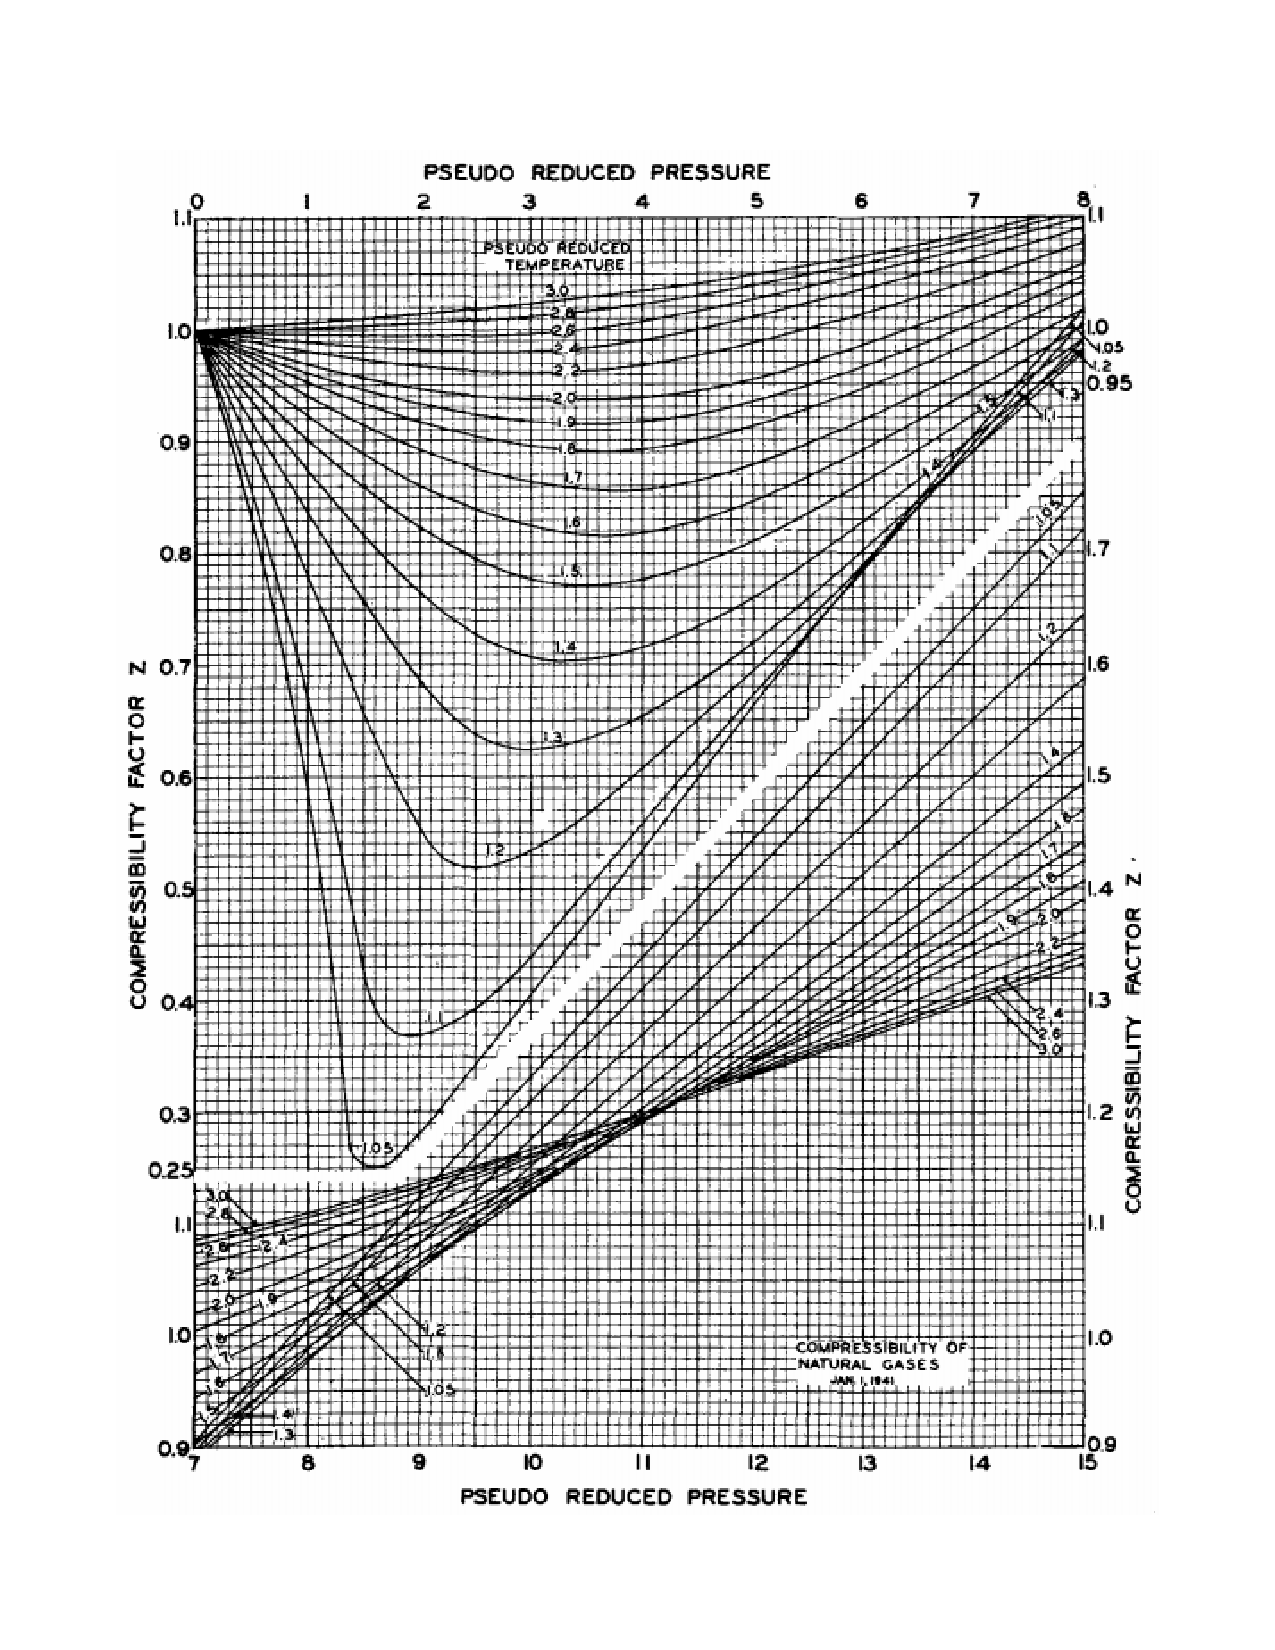
\includegraphics[width=0.70\columnwidth]{images/StandingKatzOriginal.pdf}
\caption{Standing and Katz \cite{StandingKatz1942} Natural Gas Mixture Z-Factor Chart.}
\label{fig:StandingKatzZFactors}
\end{figure}

\begin{figure}[ht]
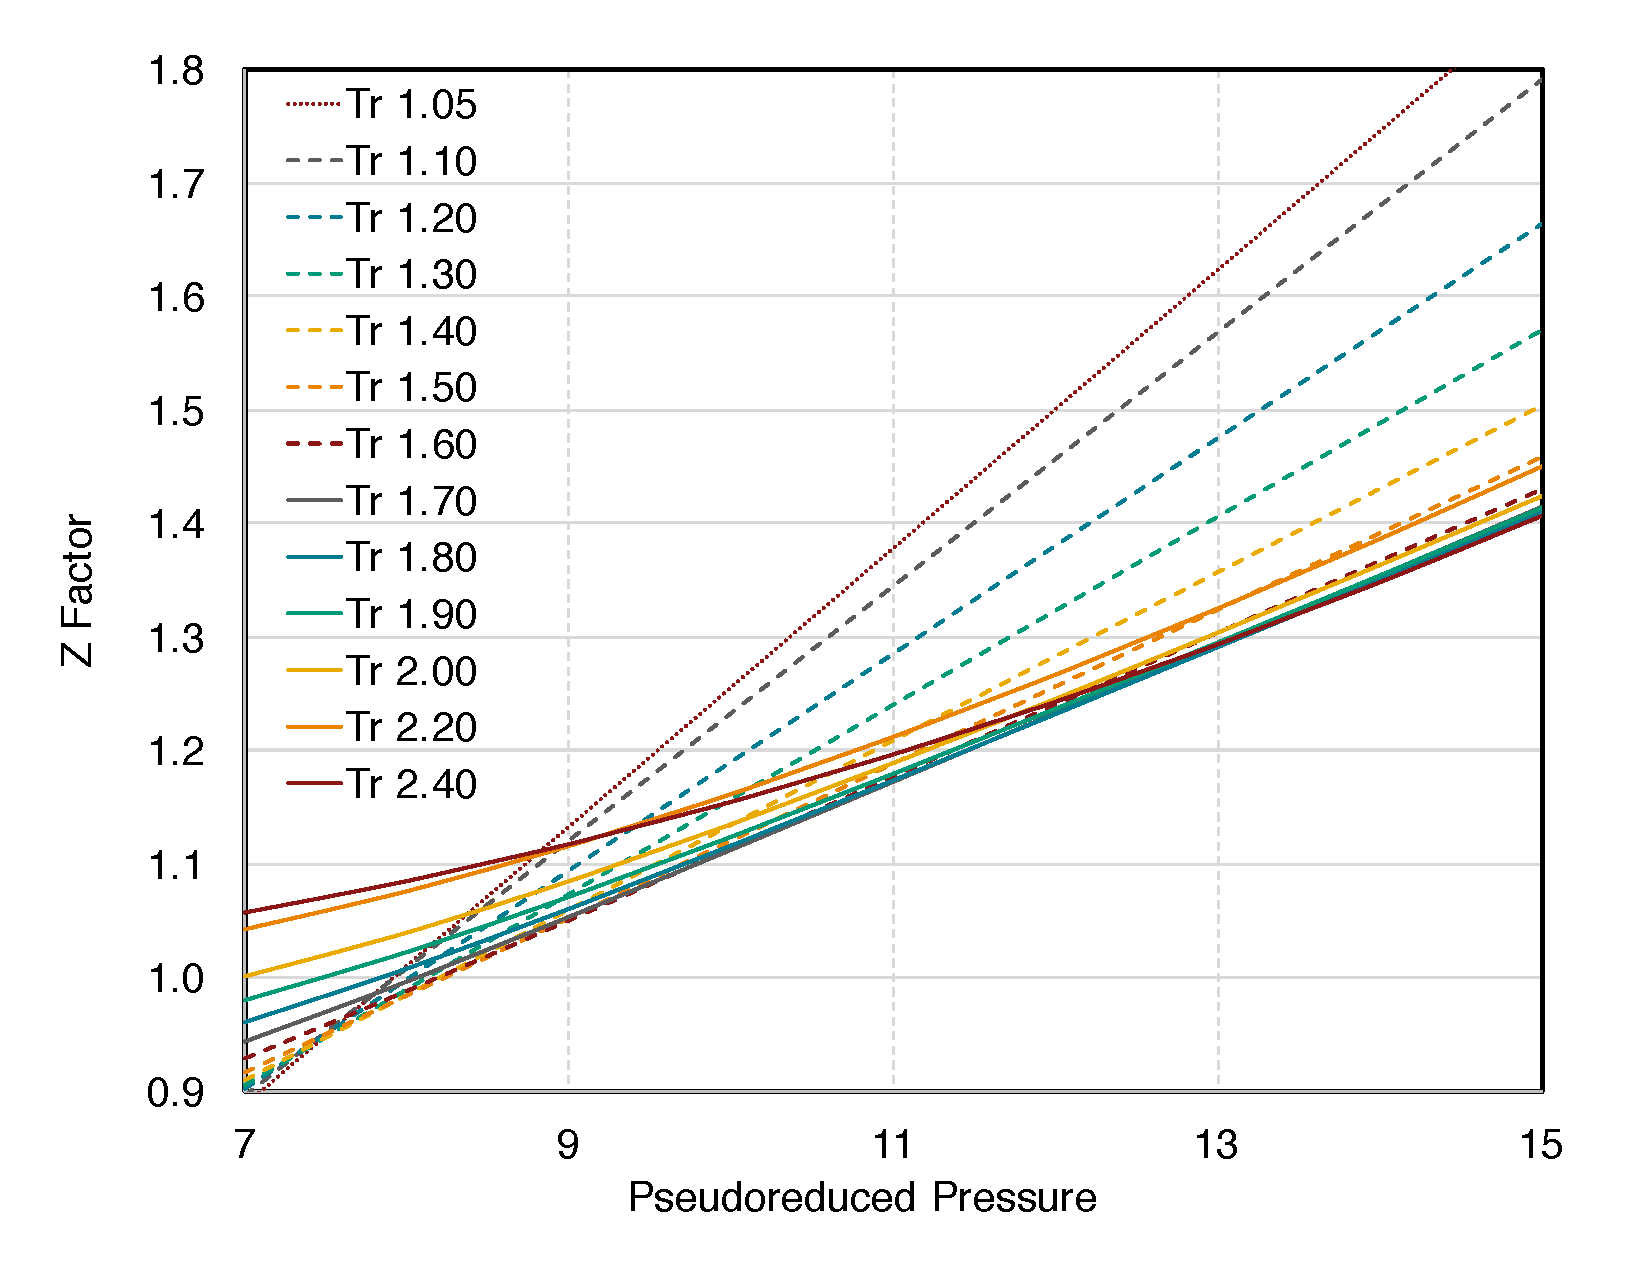
\includegraphics[width=0.70\columnwidth]{images/StandingKatzCorrelationUpper.pdf}
\caption{Correlation of Upper Portion of Standing and Katz Z-Factor Chart. Source: \cite{Standing1977}.}
\label{fig:SBBCorrelationUpper}
\end{figure}

\begin{figure}[ht]
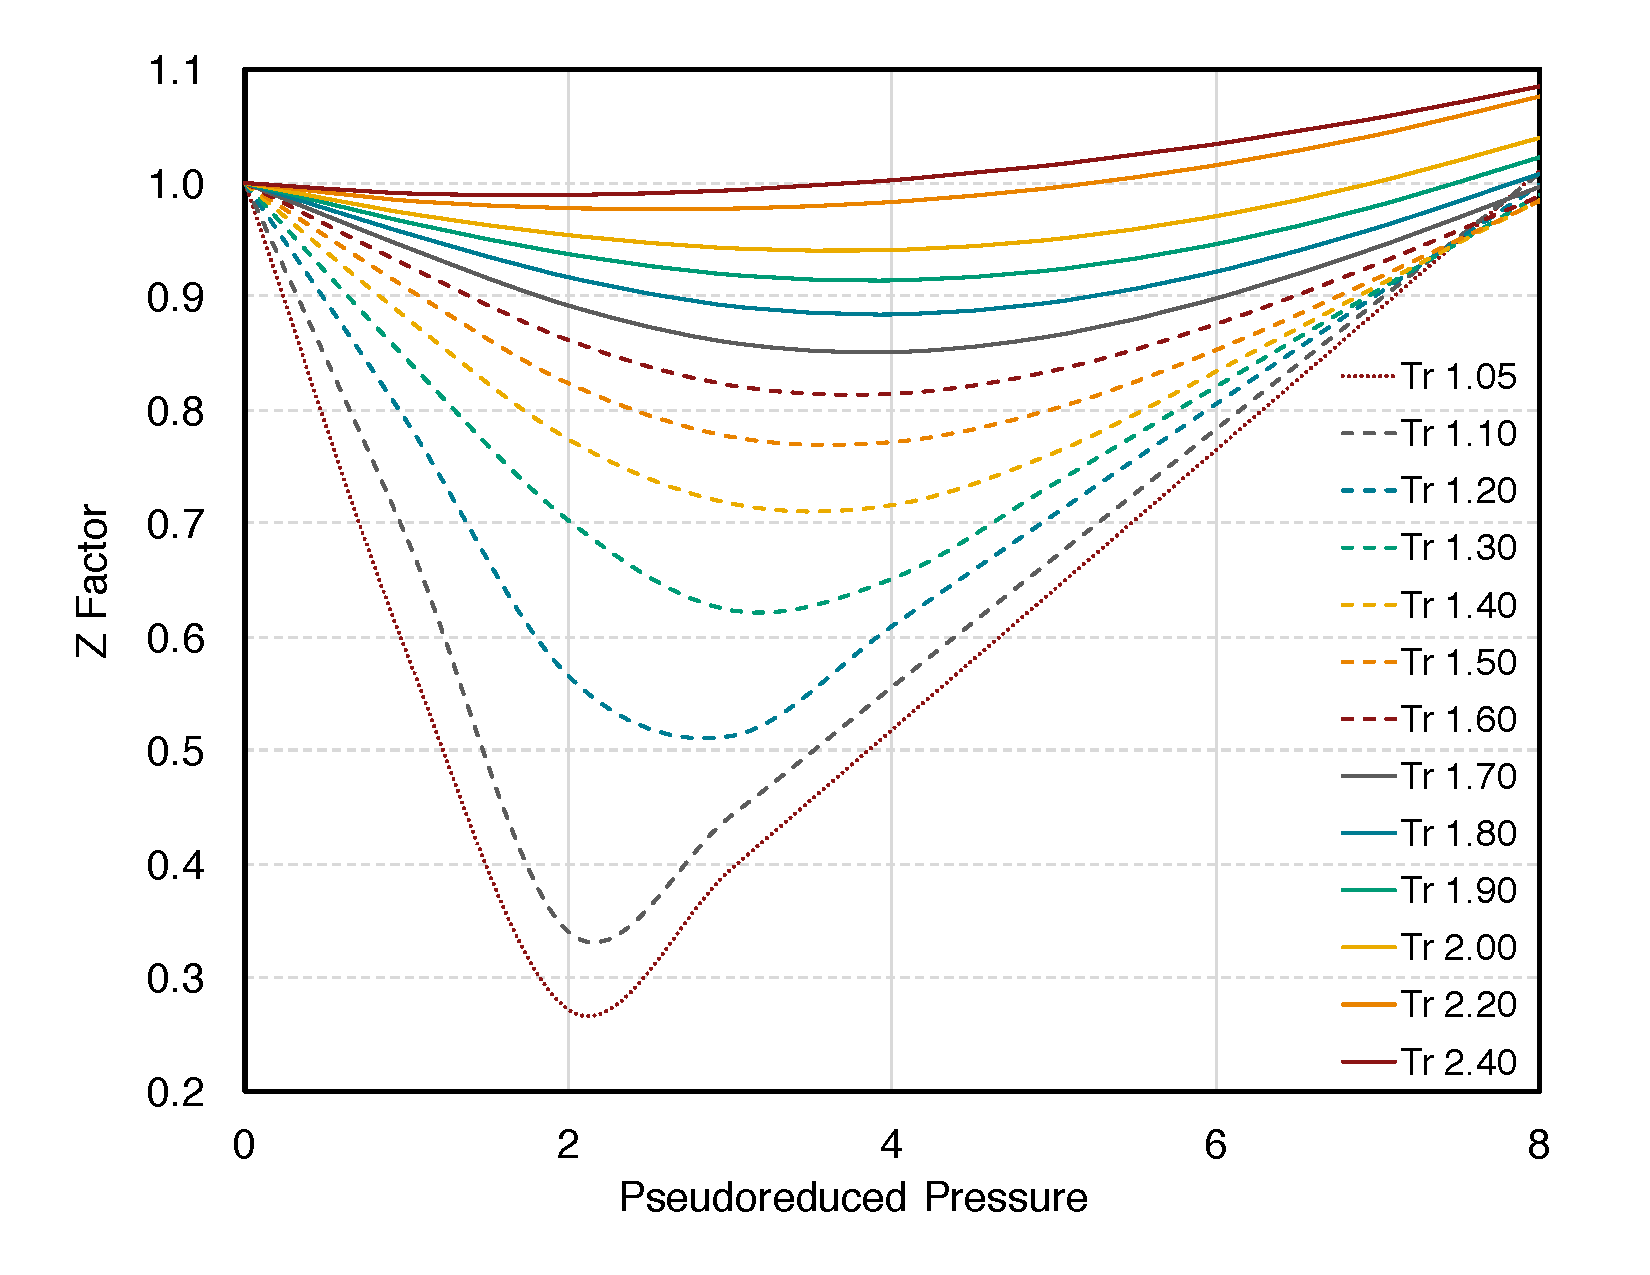
\includegraphics[width=0.70\columnwidth]{images//StandingKatzCorrelationLower.pdf}
\caption{Correlation of Lower Portion of Standing and Katz Z-Factor Chart. Source: \cite{Standing1977}.}
\label{fig:SBBCorrelationLower}
\end{figure}



\paragraph{Gas formation volume factor}

The gas formation volume factor \xlname{GVF} is the ratio of the volume of gas at the temperature and pressure of the stream in question to the volume of the same amount (moles) of gas at standard conditions.

Given the Z-factor computed above \xlname{Z\_FACTOR}, the gas volume ratio can be computed as:

\begin{minipage}{0.6\columnwidth}
\begin{fleqn}[0pt]
\begin{equation}
FVF_g= \frac{Z p_{0} T}{p T_{0}} \eqnunitfrac{m$^3$}{std m$^3$}
\end{equation}
\end{fleqn}
\end{minipage}\hfill
\begin{minipage}{0.3\columnwidth}
        \begin{tabular}{|cl}
        & \\
        $p_0$   & \xlname{Amb\_press}\\
        $T_0$   & \xlname{Amb\_temp}\\
        & \\
        \end{tabular}
\end{minipage}

where $T$ is the absolute temperature of the stream [$^\circ$R], $T_0$ is the ambient absolute temperature \xlname{Amb\_temp} [$^\circ$R], $p$ is the pressure of the stream [psia] and $p_0$ is ambient pressure [psia] \xlname{Amb\_press}.

\paragraph{Gas density}

Gas density \xlname{RHO\_G} is given by the MW of gas relative to air, the density of air at standard conditions, and the gas formation volume factor:

\begin{minipage}{0.6\columnwidth}
\begin{fleqn}[0pt]
\begin{equation}
\rho_g = \frac{\rho_{air}\gamma_g}{FVF_g}  \eqnunitfrac{tonne}{m$^3$}
\end{equation}
\end{fleqn}
\end{minipage}\hfill
\begin{minipage}{0.3\columnwidth}
        \begin{tabular}{|cl}
        & \\
        $\rho_g$   & \xlname{RHO\_G}\\
        & \\
        \end{tabular}
\end{minipage}

\paragraph{Gas molecular weight}

The molecular weight of the gas in a particular stream \xlname{MW\_G} is given by the mole-fraction-weighted molecular weight of species in the stream:
\begin{equation}
MW_g = \sum_i x_i MW_i \quad\quad\eqnunitfrac{g}{mol}
\end{equation} 
where $x_i$ is the mole fraction of species $i$ -- \xlname{MOL\_FRAC\_N2} $\ldots$ \xlname{MOL\_FRAC\_SO2} -- and $MW_i$ is the molecular weight of species $i$ [g/mol].

\paragraph{Gas volumetric flow rate}
The volumetric flow rate of gas per day \xlname{Q\_G} [m$^3$/d] is given by:

\begin{minipage}{0.6\columnwidth}
\begin{fleqn}[0pt]
\begin{equation}
Q_g = \frac{m_{tot,g}}{\rho_g} 	\eqnunitfrac{m$^3$}{d}
\end{equation}
\end{fleqn}
\end{minipage}\hfill
\begin{minipage}{0.3\columnwidth}
        \begin{tabular}{|cl}
        & \\
        $Q_g$    & \xlname{Q\_G}\\
        $\rho_g$   & \xlname{RHO\_G}\\
        & \\
        \end{tabular}
\end{minipage}

\paragraph{Gas energy density}

The energy density of the gas \xlname{LHV\_G} \xlname{LHV\_G\_lb} is given by the mass-fraction weighted energy densities of the species:

\begin{minipage}{0.6\columnwidth}
\begin{fleqn}[0pt]
\begin{equation}
 LHV_g = \frac{\sum_{1}^{12} m_i LHV_i }{\sum_{1}^{12} m_i}	\eqnunitfrac{MJ}{kg}
\end{equation}
\end{fleqn}
\end{minipage}\hfill
\begin{minipage}{0.3\columnwidth}
        \begin{tabular}{|cl}
        & \\
       \emph{LHV$_g$}   & \xlname{LHV\_G}\\
        & \\
        \end{tabular}
\end{minipage}

where $m_i$ is the mass of gas species $i$ and $LHV_i$ is the lower heating value (mass-specific) looked up from the \sheet{Fuel specs} sheet.

 \paragraph{Total gas energetic flow rate}
 
 The total gas energetic flow rate for a given stream is given by:
 
\begin{minipage}{0.6\columnwidth}
\begin{fleqn}[0pt]
\begin{equation}
 Q_{LHV,g} = m_{tot,g} LHV_g \quad\quad\eqnunitfrac{m$^3$}{d}
\end{equation}
\end{fleqn}
\end{minipage}\hfill
\begin{minipage}{0.3\columnwidth}
        \begin{tabular}{|cl}
        & \\
       \emph{LHV$_g$}   & \xlname{LHV\_G}\\
        & \\
        \end{tabular}
\end{minipage}
 
 \subsection{Properties of water}
 
 \paragraph{Specific gravity of water}

The specific gravity of produced water (\xlname{GAMMA\_W}) at standard conditions is calculated using \cite[p. 481]{Fanchi2007}: 
%%%%%%%%%%

\begin{minipage}{0.6\columnwidth}
\begin{fleqn}[0pt]
\begin{equation}
\gamma _{w}=1+C _{sd} 0.695 \times 10^{-6} \eqnunit{-}
\end{equation}
\end{fleqn}
\end{minipage}\hfill
\begin{minipage}{0.3\columnwidth}
        \begin{tabular}{|cl}
        & \\
       $\gamma_{w}$  & \xlname{GAMMA\_W}\\
        & \\
        \end{tabular}
\end{minipage}

%%%%%%%%%% 
where $C _{sd}$ = concentration of dissolved solids (also known as TDS) [\unitfrac{mg}{L}]. The constant 0.695 $\times$ 10$^{-6}$ has units of [\unitfrac{L}{mg}].


\paragraph{Water formation volume factor}

The water formation volume factor \xlname{WVF} is assumed to be 1.0 for all streams. Because water is nearly incompressible, equations for $B_w$ nearly always produce values near 1 (i.e., 1.03), so we reduce model complexity and requirements for iterative calculations by fixing $B_w$ to 1.0 regardless of stream temperature and pressure.

\paragraph{Water density}
Water density \xlname{RHO\_W} is given by the specific gravity of water and the water formation volume factor:

\begin{minipage}{0.6\columnwidth}
\begin{fleqn}[0pt]
\begin{equation}
\rho_w = \frac{\gamma _{w} \rho_{w,0}}{B_w} \eqnunitfrac{tonne}{m$^3$}.
\end{equation}
\end{fleqn}
\end{minipage}\hfill
\begin{minipage}{0.3\columnwidth}
        \begin{tabular}{|cl}
        & \\
        $\rho_w $   & \xlname{RHO\_W}\\
        $\gamma _{w}$   & \xlname{GAMMA\_W}\\
        & \\
        \end{tabular}
\end{minipage}

where $\rho_{w,0}$ is the density of pure water [1000 kg/m$^3$]. Because we assume $B_w$ = 1 for simplicity, $\rho_w = \gamma _{w} \rho_{w,0}$. 

\paragraph{Water flow rate}
Water flow rate \xlname{Q\_W} is computed from mass flow rate of water $m_w$ for a given stream and the density of water $\rho_w$ for that stream:

\begin{minipage}{0.6\columnwidth}
\begin{fleqn}[0pt]
\begin{equation}
Q_w = \frac{m_w}{\rho_w} \eqnunitfrac{m$^3$}{d}
\end{equation}
\end{fleqn}
\end{minipage}\hfill
\begin{minipage}{0.3\columnwidth}
        \begin{tabular}{|cl}
        & \\
        $Q_w$   & \xlname{Q\_W}\\
         $\rho_w $   & \xlname{RHO\_W}\\
        & \\
        \end{tabular}
\end{minipage}

This water flow rate is also converted to bbl \xlname{Q\_W\_bbl} and ft$^3$ \xlname{Q\_W\_ft3} for simplicity of interpretation.


\section{Process flow diagram}

Below the \xlname{FlowTable} lies diagrammatic illustration of the process modules presented in OPGEE and their interconnection with streams. An overall map of the process flow diagram (PFD) is given in Figure \ref{fig:PFD_map}. In general, the following colors are used to present different types of flows:
\begin{itemize}
    \item Green: Oil, diluent, bitumen, LPG
    \item Red: Gas
    \item Blue: Water
    \item Yellow: Electricity
    \item Black: Petroleum coke and raw bitumen
    \item Other: Non-hydrocarbon gases for injection (e.g., N$_2$ flooding) 
\end{itemize}

\begin{landscape}
\begin{figure}[t]
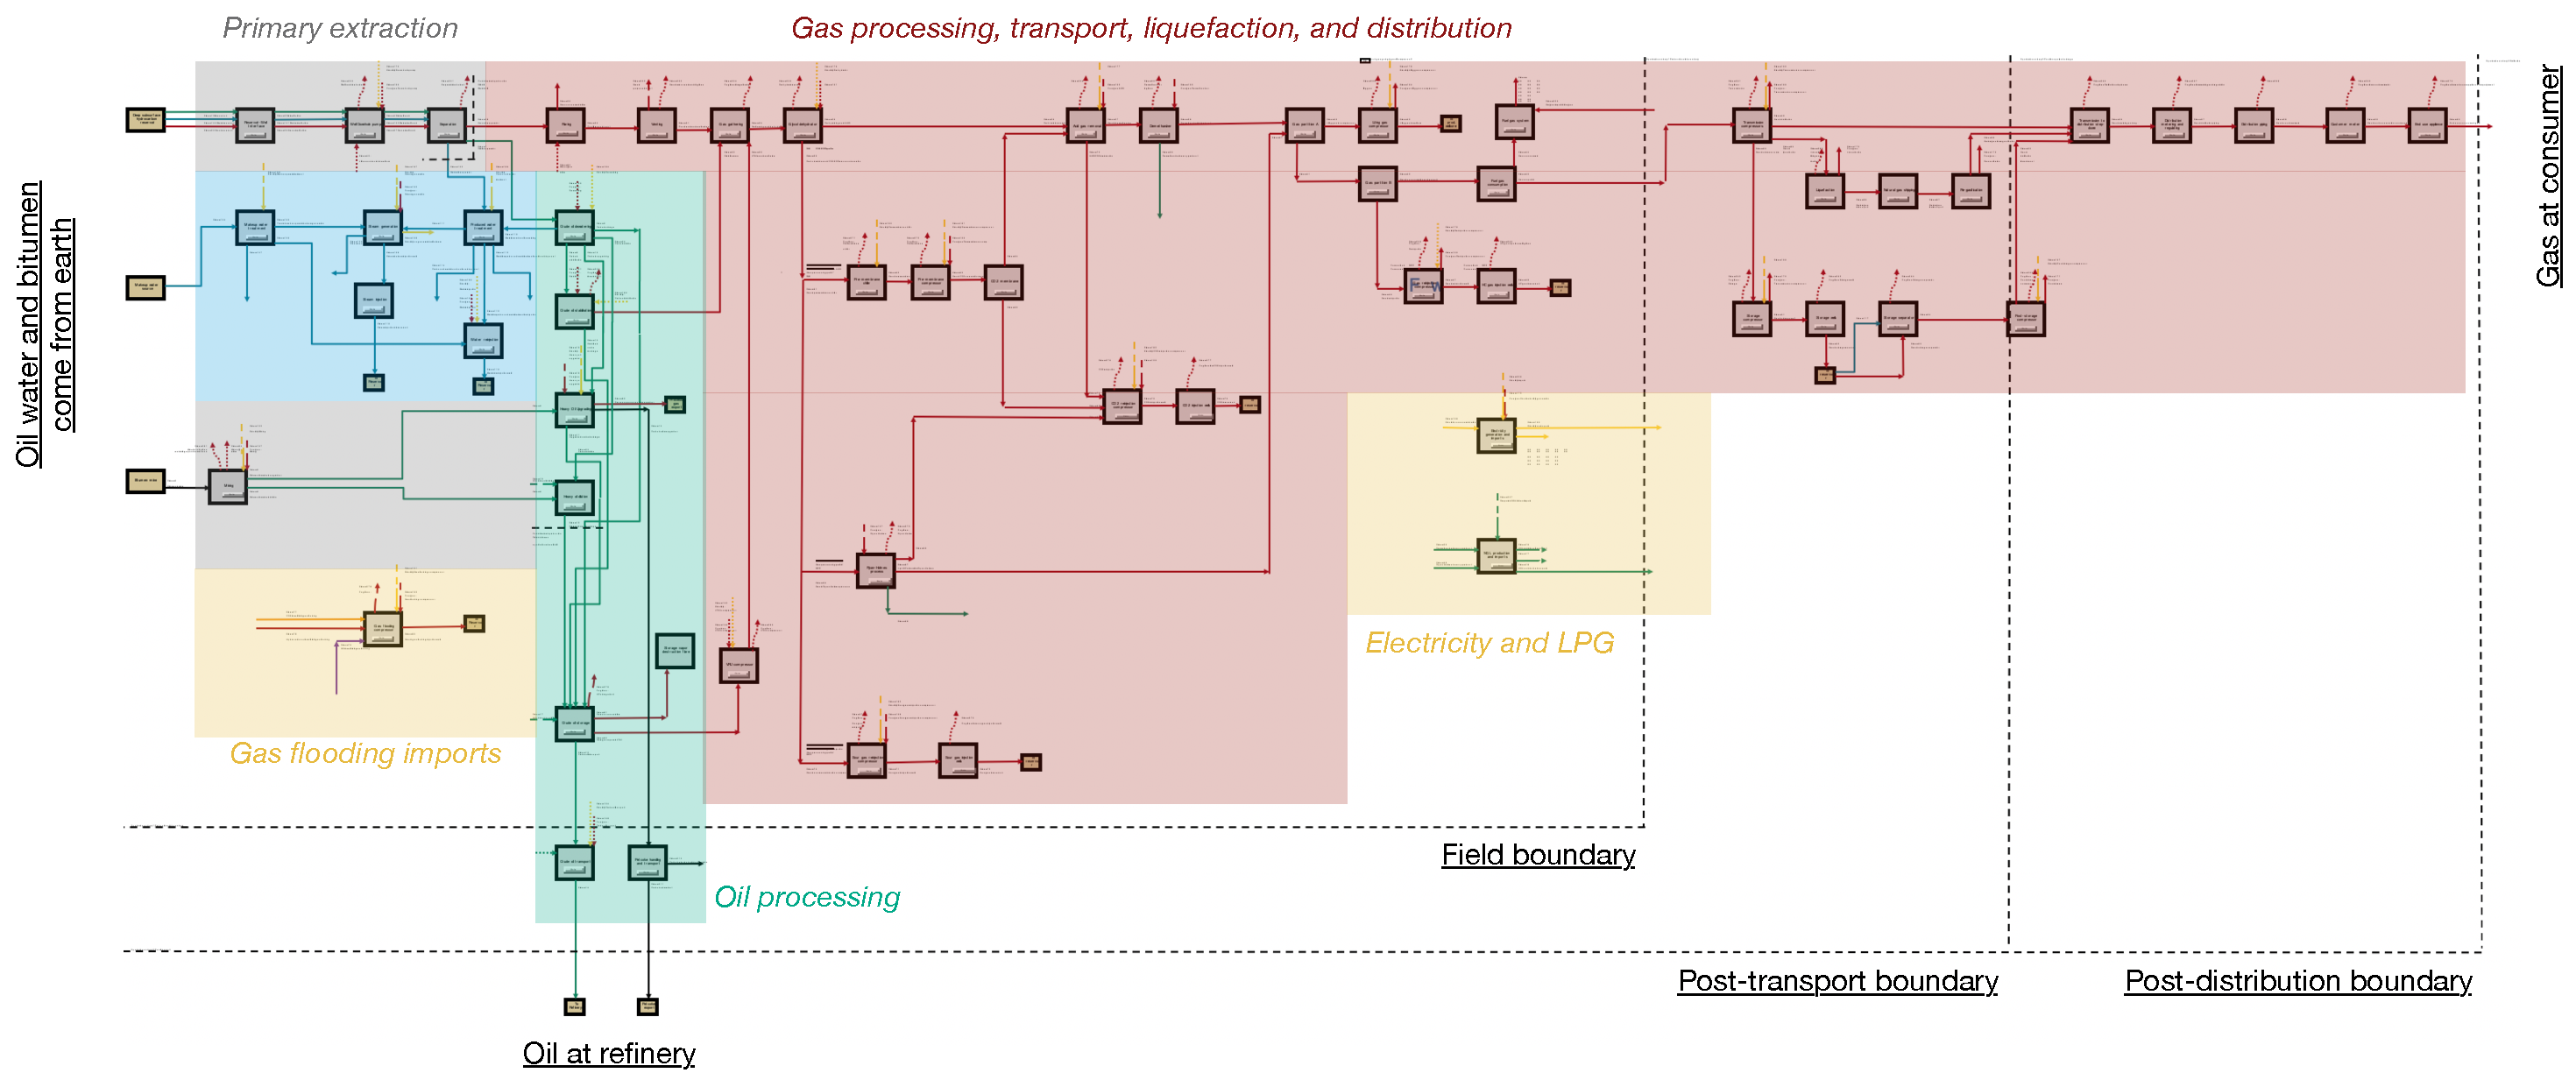
\includegraphics[width=1\columnwidth]{images/PFD_map.pdf}
\caption{Process flow diagram at maximum zoom, showing color-coded regions with each major stream type being processed in that region.}
\label{fig:PFD_map}
\end{figure}
\end{landscape}

Each process module can be examined more closely. Figure \ref{fig:Process_mod_diagram} below shows the ``up-close'' version of a process model along with its important elements. Entering streams have an arrow entering the module box, while leaving streams have arrows leaving. Entering streams that become dashed far away from the box are remote streams that come from elsewhere on the PFD but are not connected directly for clarity of presentation. Fugitive streams leaving are curved dashed lines. The ``Go to'' button allows you to jump directly to that process model. The operation indicator is always to the upper left of the process box and is the main place where the operation or non-operation is recorded (i.e., this directly calls from the \sheet{Active field} sheet and is used in downstream calculations). 

\begin{figure}[t]
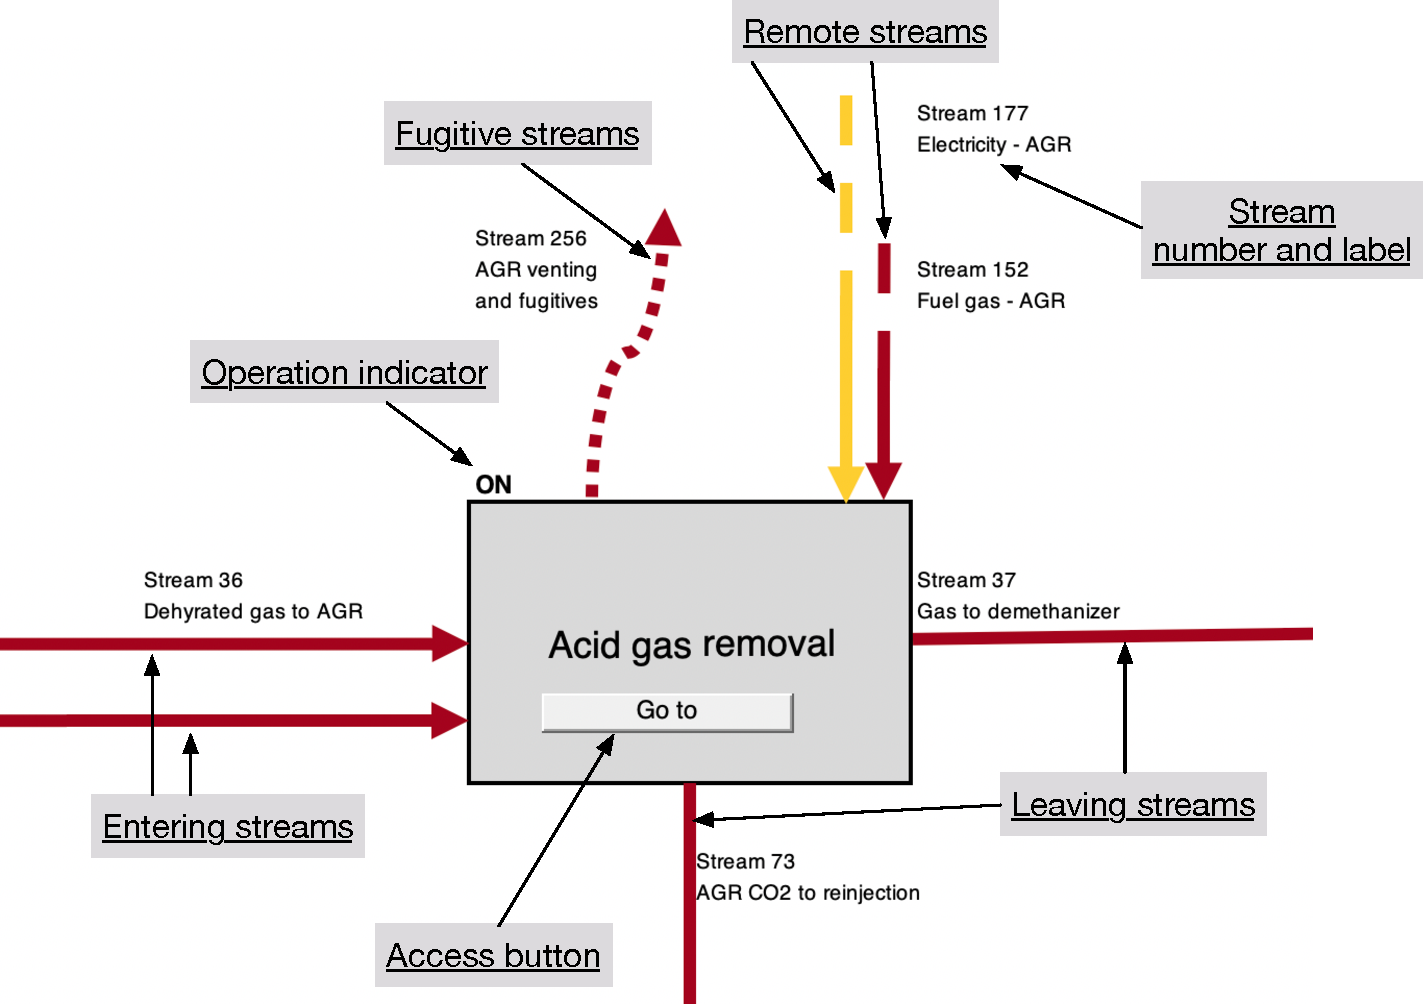
\includegraphics[width=1\columnwidth]{images/Process_mod_diagram.pdf}
\caption{Process module up close showing important elements.}
\label{fig:Process_mod_diagram}
\end{figure}


%%%%%%%%%%%%%%%%%%%%%%%%%%%%%%%%%%%%%%%%%%%%%
%%%%%%%%%%%%%%%%%%%%%%%%%%%%%%%%%%%%%%%%%%%%%
%%%%%%%%%%%%%%%%%%%%%%%%%%%%%%%%%%%%%%%%%%%%%

\chapter{Gathering worksheets}

This section explains three worksheets in OPGEE which are used to collect output from intermediate calculations in process stage and supplemental worksheets. This collected output is used to calculate the overall WTR energy consumption and GHG emissions of the study crude. These gathering worksheets are the \sheet{Energy Summary}, \sheet{GHG Summary}, and \sheet{Active Field} worksheets. 


\clearpage

%%%%%%%%%%%%%%%%%%%%%%%%%%%%%%%%%%%%%
\section{\sheet{Energy Summary} gathering worksheet}\label{sec:energy_consumption}

In the \sheet{Energy Summary} gathering worksheet, energy use is summed in order of process stages, from Exploration to Waste disposal. Table 1 on the \sheet{Energy Summary} sheet gathers energy use for all process worksheets. For consistency, all energy inputs are summed on a daily basis, either as thermal energy [mmBtu/d] or as electrical energy [kWh/d]. 

Table 2 on the \sheet{Energy Summary} sheet summarizes in simpler form the consumption for each fuel. 

In Table 3, the energy exports/imports are calculated by fuel type. Energy exports/imports are used to calculate indirect (offsite) energy consumption and GHG emissions by fuel type. Indirect energy consumption and GHG emissions are associated with the production and transport (production only in case of exports) of the fuel consumed directly. 

For example, the exports/imports of natural gas are calculated as: 
\begin{equation}
E_{ng,exp} = E_{ng,gr} - E_{ng,fuel} + E_{ng,mu} - E_{ng,rec} \quad\quad\eqnunitfrac{mmBtu}{d}
\end{equation}
where $E_{ng,exp}$ = natural gas export/import [mmBtu/d]; $E_{ng,gr}$ = gross natural gas consumption [mmBtu/d]; $E_{ng,fuel}$ = natural gas produced as fuel after gas lifting/re-injection [mmBtu/d]; $E_{ng,mu}$ = make up natural gas for gas flooding [mmBtu/d], if applicable; and $E_{ng,rec}$ = natural gas recovered from venting and fugitives. The produced gas remaining to be used as a process fuel is equal to 0 mmBtu/d in the case of gas flooding where 100\% of produced gas is re-injected. Negative $E_{ng,exp}$ represents gas exports. Positive $E_{ng,exp}$ represents gas imports.

The exports/imports of natural gas liquid (NGL) is calculated as:
\begin{equation}
E_{ngl,exp} = E_{ngl,gr} - E_{ngl,fuel} \quad\quad\eqnunitfrac{mmBtu}{d}
\end{equation}
where $E_{ngl,exp}$ = NGL export/import [mmBtu/d]; $E_{ngl,gr}$ = gross NGL consumption [mmBtu/d]; and $E_{ngl,fuel}$ = amount of NGL produced as fuel [mmBtu/d]. 

Note that Table 3 contains an indicator for whether displacement is used to allocate emissions for a given export stream or not. This is used in accounting for \sheet{Active Field} and \sheet{Results} sheet display, and is controlled in the control at the top of the \sheet{Inputs} sheet.

In Table 4, the indirect energy consumption by fuel type is calculated. Indirect energy consumption refers to offsite use of energy to supply the energy inputs consumed as net imports (and the opposite for exports). Indirect energy consumption is calculated as:
\begin{equation}
\begin{split}
& E_{k,ind} = E_{k,exp} \, E_{k,FC} \quad\quad \text{for}\,\, E_{k,exp} > 0\\
& E_{k,ind} = E_{k,exp} \, E_{k,DS} \quad\quad \text{for}\,\, E_{k,exp} < 0 \,\,\text{and displacement}\\ 
& E_{k,ind} = 0 \quad\quad\quad\quad\quad\quad\,\, \text{for}\,\, E_{k,exp} < 0 \,\,\text{and allocation by energy value}\\
\end{split}
\end{equation}
where $k$ refers to the fuel type; $E_{k,ind}$ = indirect energy consumption [mmBtu/d]; $E_{k,exp}$ = fuel export/import [mmBtu/d]; $E_{k,FC}$ = fuel cycle energy consumption [mmBtu/mmBtu]; and $E_{k,DS}$ = energy consumption of displaced system in case of fuel export [mmBtu/mmBtu]. For more details on the energy consumption of fuel cycles and displaced systems, see Section \ref{sec:fuel_cycle}.

Table 5 summarizes embodied energy contained in oilfield materials such as steel and cement that are used during development of the field. These calculations are performed in detail on the \sheet{Embodied Emissions} sheet, and only summarized here.

Lastly, Table 6 in the \sheet{Energy Summary} worksheet creates the total energy output for the denominator of LCA equations. The total primary energy output is either the oil or natural gas output from Table 3, depending on which product is selected as the primary product. Secondary products also exported are summarized here if applicable [mmBtu/d]. The heating value basis (LHV or HHV) for these products is as selected on the \sheet{Inputs} worksheet. \\

If the division of environmental impacts between co-products is done by energy value allocation and not co-product displacement (again, selected on \sheet{Inputs} sheet), the energy content of the co-products is added to the denominator of the CI calculation.

The final row of Table 6, ``Denominator for computing CI'' is the main result of the sheet, and is used downstream in calculations on the \sheet{Active Field} and \sheet{Results} sheets.




\clearpage

%%%%%%%%%%%%%%%%%%%%%%%%%%%%%%%%%%%%%
\section{\sheet{GHG Summary} gathering worksheet}\label{sec:GHG_emissions}

The GHG emissions gathering worksheet compiles and computes emissions of all emissions types across all process stages. The first step is the compilation of direct GHG emissions from the different worksheets of the model. These emissions are computed at the bottom of each of the process sheets, and saved as a vector of the following format:
\begin{itemize}
\item Combustion emissions from use of fuels on site
\item Land use emissions 
\item Venting emissions (part of ``VFF'')
\item Flaring emissions (part of ``VFF'')
\item Fugitive emissions (part of ``VFF'')
\end{itemize}

On each worksheet, these different elements are computed as follows:
\paragraph{Combustion emissions}
Combustion emissions are computed by taking the ``Energy use'' vector that is at the bottom of each worksheet and summing the product of each energy use amount in mmbtu/d by the emissions intensity for that energy use in g CO$_2$eq. GHG per mmbtu of energy consumed. These emissions intensity vectors are contained on the \sheet{Emissions Factors} sheet, and described below. In simple terms, each process sheet has an assumed mix of combustion devices, which governs the emissions resulting from, say, burning 1 mmbtu of natural gas. Because different process stages may use different mixes of equipment, the emissions factors for each process stage may differ slightly.

\paragraph{Land use emissions}
These emissions are set equal to 0 except for the \sheet{Drilling \& development} sheet, which counts the land use impacts of land clearing and conversion. See section \ref{sec:drilling} below for description of these calculation methods and the sources upon which they rely.

\paragraph{Venting}
Venting emissions are computed at the bottom of each sheet by taking each venting mass flow vector of vented gases and computing the GWP-weighted amount of CO$_2$ equivalent emissions using the defined values \xlname{GWP\_CH4}, \xlname{GWP\_VOC}, and \xlname{GWP\_CO} for methane, VOCs, and carbon monoxide, respectively. These values are stored on the \sheet{Constants} sheet.

The actual computation methods for computing masses of gas species vented for each process unit is described in detail in section \ref{sec:VFF} below.

\paragraph{Flaring}
Flaring emissions are set equal to zero except for the \sheet{Flaring} sheet, which is described in detail below in section \ref{sec:flaring}.

\paragraph{Fugitives}
Fugitive emissions are computed at the bottom of each sheet by taking each venting mass flow vector of fugitive gases and computing the GWP-weighted amount of CO$_2$ equivalent emissions using the defined values \xlname{GWP\_CH4}, \xlname{GWP\_VOC}, and \xlname{GWP\_CO} for methane, VOCs, and carbon monoxide, respectively. These values are stored on the \sheet{Constants} sheet.

The actual computation methods for computing masses of gas species fugitives for each process unit is described in detail in section \ref{sec:VFF} below.

The next step is the calculation of indirect GHG emissions resulting from net fuel imports or exports, if displacement-based methods are applied. The indirect GHG emissions are calculated as:
\begin{equation}
\begin{split}
& EM_{k,ind} = E_{k,exp} \, EM_{k,FC} \quad\quad \text{for}\,\, E_{k,exp} > 0\\
& EM_{k,ind} = E_{k,exp} \, EM_{k,DS} \quad\quad \text{for}\,\, E_{k,exp} < 0 \,\,\text{and displacement}\\
& EM_{k,ind} = 0 \quad\quad\quad\quad\quad\quad \text{for}\,\, E_{k,exp} < 0 \,\,\text{and allocation by energy value}\\
\end{split}
\end{equation} 
where $k$ refers to the fuel type; $EM_{k,ind}$ = indirect GHG emissions from fuel consumption [gCO$_{2}$eq/d]; $E_{k,exp}$ = fuel export/import [mmBtu/d]; $EM_{k,FC}$ = fuel cycle GHG emissions [gCO$_{2}$eq/mmBtu]; and $EM_{k,DS}$ = GHG emissions from displaced system in case of fuel export [gCO$_{2}$eq/mmBtu]. For details on the GHG emissions of fuel cycles and displaced systems, see section \ref{sec:fuel_cycle}.

Next, the GHG emissions gathering worksheet considers the impact  of CO$_2$ sequestration. Sequestration-related calculations are applicable only if gas flooding is selected as a production practice and CO$_2$ is selected as the flood gas. 

The CO$_2$ sequestration credited to the oilfield is included in the overall calculations in the \sheet{Results} worksheet. It is calculated by first considering the source of the CO$_2$. If the CO$_2$ was acquired from a naturally occurring subterranean source then no sequestration credit accrues because this CO$_2$ was already sequestered. A sequestration credit is applicable only if the CO$_2$ originated from an anthropogenic source --- it must have been captured during industrial process such as coal combustion. 

Furthermore, depending on the specific regulations and laws governing CO$_2$ sequestration, the credit may accrue either to the CO$_2$ capturing facility or to the oilfield operator injecting it into a reservoir. OPGEE also deducts CO$_2$ that is released due to long-term reservoir leakage and an oilfield operator's decision to conduct terminal phase blow-down operations. OPGEE's consideration of long-term leakage and operator blow-down is described in Section \ref{sec:Sequestration}.

If the carbon dioxide used for EOR is anthropogenic, then the overall CO$_2$ sequestration credit accruing to the oilfield is calculated as:
%%%%%%%%%%
\begin{equation} \label{eq:SequestrationCredit}
CR_{CO_{2}} = P_{oilfield} \cdot (Seq_{CO_{2}} - Blow_{CO_{2}} - Leakage_{CO_{2}}) \quad\quad\eqnunitfrac{gCO$_2$}{d}
\end{equation}
%%%%%%%%%%
 where $CR_{CO_{2}}$ = CO$_2$ sequestration credit assigned to the oilfield [gCO$_2$/d]; $P_{oilfield}$ = proportion of the overall sequestration credit assigned to the oilfield [-]; $Seq_{CO_{2}}$ = CO$_2$ sequestration rate [gCO$_2$/d]; $Blow_{CO_{2}}$ = CO$_2$ lost from the reservoir from terminal blow-down operations [gCO$_2$/d]; and $Leakage_{CO_{2}}$ = the amount of CO$_2$ leaving the reservoir from long-term leakage [gCO$_2$/d].
 
Next, embodied emissions are summarized. These embodied emissions are computed on the \sheet{Embodied emissions} sheet, and described in detail in section \ref{sec:embodied_emissions} below.

Lastly, a summary emissions credit or debit for offsite activities is computed at the bottom of the \sheet{GHG Summary} sheet. This is used on the \sheet{Active Field} sheet for further computation of offsite debits and credits per MJ of fuel exported.



%%%%%%%%%%%%%%%%%%%%%%%%%%%%%%%%%%%%%%%%%%%%%
%%%%%%%%%%%%%%%%%%%%%%%%%%%%%%%%%%%%%%%%%%%%%
%%%%%%%%%%%%%%%%%%%%%%%%%%%%%%%%%%%%%%%%%%%%%

\chapter{Process worksheets}

This section explains the main assumptions and calculations for each process worksheet. Items discussed include user assumptions and choices, process calculation assumptions, calculations of input parameters, and calculations of intermediate outputs.


\clearpage
%%%%%%%%%%%%%%%%%%%%%%%%%%%%%%%%%%%%%%%%%%%%%
\section{Exploration}\label{sec:exploration}

Emissions from petroleum exploration occur during clearing of land for seismic surveys, operation of seismic survey equipment, drilling of exploratory wells, and from fugitive emissions during drilling operations. Offsite emissions occur due to other materials and services consumed during drilling (e.g., computing energy consumed during seismic data processing). A complete list of emissions sources, along with their categorization and estimated magnitude, is shown in Table \ref{tab:exploration_sources}.

Inputs for exploration emissions from the \sheet{Inputs} sheet (gathered from the \sheet{Active Field} worksheet) include:
\begin{itemize}
\item Field depth \xlname{Field\_depth} [ft]
\item Is field offshore \xlname{Offshore\_01} [0-1]
\item Field production rate \xlname{Oil\_prod} [bbl/d]
\end{itemize}

Inputs on the \sheet{Secondary Inputs} sheet include:
\begin{itemize}
\item Distance of travel for survey \xlname{Distance\_survey} [mi]
\item Weight of land survey vehicle \xlname{Weight\_land\_survey} [tons]
\item Weight of ocean survey vehicle \xlname{Weight\_ocean\_survey} [tons]
\item Dry holes drilled per field found \xlname{Number\_wells\_dry} [\# wells]
\item Exploratory or scientific wells drilled after field discovery (non-producing) \xlname{Number\_wells\_exploratory} [\# wells]
\end{itemize}
The default values for these inputs are noted in Table \ref{tab:exploration}.

\subsection{Calculations for petroleum exploration}

The survey vehicle energy consumption (e.g., seismic survey ship or seismic survey trucks) are calculated as:

%%%%%%%%%%%%EQ%%%%%%%%%%%%%%%%%
\begin{minipage}{0.6\columnwidth}
\begin{fleqn}[0pt]
\begin{equation}\label{eq:explore_Eexp}
E_{EXP,s} = \sum_{j \in S,T} y_j \cdot m_j \cdot D \cdot EI_{j}  \eqnunit{mmBtu}
\end{equation}
\end{fleqn}
\end{minipage}\hfill
\begin{minipage}{0.3\columnwidth}
        \begin{tabular}{|cl}
        $y_j$   	& \xlname{Offshore\_01}\\
         $m_j $   	& \xlname{Weight\_land\_survey}\\
         		& \xlname{Weight\_ocean\_survey}\\
	$D$		& \xlname{Distance\_survey}	\\
	$EI_j$	& - \\
        \end{tabular}
\end{minipage}
%%%%%%%%%%%%EQ%%%%%%%%%%%%%%%%%%

where $y_j$ \xlname{Offshore\_01} is a binary variable representing whether exploration mode $S$ (ship-based exploration) or $T$ (truck-based exploration) is performed [-]; $m_j$ is the weight of exploration vehicle $j$ [ton] \xlname{Weight\_land\_survey}, \xlname{Weight\_ocean\_survey}; $D$ is the distance traveled by exploration vehicle [mi] \xlname{Distance\_survey}; and $EI_{j}$ is the energy-intensity of transport type $j$ [Btu/ton-mi], as computed on the \sheet{Transport} worksheet.

Energy consumed in drilling exploratory wells is computed using drilling energy intensity computed on the \sheet{Drilling \& Development} sheet. The drilling energy consumption for exploratory and dry wells is computed as follows:

%%%%%%%%%%%%EQ%%%%%%%%%%%%%%%%%
\begin{minipage}{0.6\columnwidth}
\begin{fleqn}[0pt]
\begin{equation}\label{eq:explore_Edrill}
E_{EXP,d} = (n_{w,d} + n_{w,exp}) \cdot EI_{w}  \eqnunit{mmBtu}
\end{equation}
\end{fleqn}
\end{minipage}\hfill
\begin{minipage}{0.3\columnwidth}
        \begin{tabular}{|cl}
        $n_{w,d}$   	& \xlname{Number\_wells\_dry}\\
        $n_{w,exp} $   	& \xlname{Number\_wells\_exploratory}\\
	$EI_w$	& - \\
        \end{tabular}
\end{minipage}
%%%%%%%%%%%%EQ%%%%%%%%%%%%%%%%%%

where $n_{w,d}$ \xlname{Number\_wells\_dry} is the number of dry wells drilled during exploration [\# wells]; $n_{w,exp}$ is the number of exploratory wells drilled during exploration (non-dry) [\# wells]; and $EI_{w}$ is the energy-intensity of drilling [mmBtu/well], as computed on the \sheet{Drilling \& development} worksheet.

Energy consumed in exploration is then expressed as a fraction of the total lifetime energy production assumed produced from the field.  This quantity is derived in the \sheet{Drilling \& Development} sheet.



\subsection{Defaults for petroleum exploration}

Table \ref{tab:exploration} shows the default settings for petroleum exploration.

% issue 4: the last two parameters of Table 7.1 do not have defined name in OPGEE secondary sheet

\begin{landscape}
\begin{table}
\begin{scriptsize}
\tablefirsthead{\toprule Param. & Description & Defined name & Eq. no. & Default & Literature range & Unit & Sources & Notes\\
\midrule}
\tablehead{ \multicolumn{5}{p{1\columnwidth}}{\textit{Continued from previous page}}\\ \toprule Param. &Description & Defined name & Eq. no. &Default & Literature range & Unit & Sources & Notes \\ 
\midrule }
\tabletail{\bottomrule \multicolumn{5}{p{1\columnwidth}}{\textit{Continued on next page...}}\\}
\tablelasttail{\bottomrule}
\tablecaption{Default inputs for exploration emissions}
\label{tab:exploration}
\begin{threeparttable}
\begin{supertabular*}{1\columnwidth}{p{0.03\columnwidth}p{0.3\columnwidth}p{0.15\columnwidth}p{0.05\columnwidth}p{0.07\columnwidth}p{0.05\columnwidth}p{0.1\columnwidth}p{0.05\columnwidth}p{0.05\columnwidth}}
$Di_{j} $ & Distance exploration mode $j$ travels  (same for $S$ and $T$)	& \xlname{Distance\_survey} & - 	& 10,000& - &[mi] & & a\\ 
$m_{S} $ & Weight of exploration ship 	& \xlname{Weight\_ocean\_survey} & - 	& 100 & - &[ton] & & b\\ 
$m_{T}$ & Weight of exploration truck & \xlname{Weight\_land\_survey} 	& - 	& 25  & - & [ton] & & c \\
$n_{w,d}$ & Number of dry wells drilled & \xlname{Number\_wells\_dry} 	& - 	& 1  & - & [\# wells] & &  \\
$n_{w,exp}$ & Number of non-dry exploratory wells drilled & \xlname{Number\_wells\_exploratory} 	& - 	& 3  & - & [\# wells] & &  \\
$EI_{S}$ & Energy intensity of exploration ship & 	& - & 24 	& -& [Btu/ton-mi] & \cite{Wang2009}&  \\
$EI_{T}$ & Energy intensity of exploration truck & 	& - & 969 	& -& [Btu/ton-mi] & \cite{Wang2009}&  \\
$EI_{w}$ & Energy intensity of drilling a well & 		& - & [var] 	&- & [mmBtu/well] & \cite{Vafi2016a}&  \\
\end{supertabular*}
\begin{tablenotes}
\item[a] Simple assumption for distance of travel to remote exploration site. Distance traveled during actual survey is assumed by default to be small compared to distance to field location.
\item[b] Simple assumption for weight of exploration ship
\item[c] Simple assumption for weight of exploration truck
\end{tablenotes}
\end{threeparttable}
\end{scriptsize}
\end{table}


\end{landscape}



%%%%%%%%%%%%%%%%%%%%%%%%%%%%%%%%%%%%%%%%%%%%%%%%
\clearpage
\section{Drilling \& development}\label{sec:drilling}

\subsection{Introduction to drilling \& development}

Drilling and development operations result in a variety of emissions. Well drilling and installation of production equipment results in on-site energy use (e.g., for rigs and other construction equipment) as well as indirect offsite energy use (e.g., embodied energy consumed to manufacture well casing). Drilling and development also results in land use impacts, which can release biogenic carbon from disturbed ecosystems and soils \cite{Yeh2010}. In addition, fugitive emissions can occur during the drilling process as emissions of hydrocarbon gas from drilling muds. 

\subsection{Calculations for drilling \& development}

The main reference for the OPGEE drilling energy use calculations is the GHGFrack model, by Vafi and Brandt \cite{Vafi2016a, Vafi2016b, Vafi2016c}. This model examines drilling energy use in some detail, and results are extracted from GHGFrack to provide tabular inputs to OPGEE. Because GHGFrack is quite complex, we avoid explicitly merging the models.

Three aspects of field drilling and development are modeled in OPGEE \version: drilling energy consumption, hydraulic fracturing energy consumption, and land use impacts. Other emissions from drilling and development -- including land clearing and site preparation, small truck traffic, ancillary energy use, embodied energy in labor -- are not explicitly modeled and therefore would be accounted for in the small sources term. The parameters and variables used in the drilling and development model equations are listed in Tables \ref{tab:primary_inputs_drilling}, \ref{tab:secondary_inputs_drilling}.

\subsubsection{Emissions from drilling}

Drilling oil wells consumes fuel. This fuel is consumed on site in prime movers like diesel engines and diesel electricity generators. These engines and generators power a variety of processes: pumping mud; applying torque to the drill string; pulling the drill string; raising, lowering and retrieving the subsurface monitoring equipment; and pressurizing and pumping cement. 

First, the number of total wells drilled is computed:

\begin{minipage}{0.6\columnwidth}
\begin{fleqn}[0pt]
\begin{equation}
n_{w,tot}= n_{wo} + n_{wi}  \quad\quad\eqnunit{Num. wells}
\end{equation}
\end{fleqn}
\end{minipage}\hfill
\begin{minipage}{0.3\columnwidth}
        \begin{tabular}{|cl}
        & \\
        $n_{wo}$   & \xlname{Num\_prod\_wells}\\
        $n_{wi}$   & \xlname{Num\_water\_inj\_wells}\\
        & \\
        \end{tabular}
\end{minipage}

Because OPGEE computes both consumption and production of energy on a daily basis, drilling energy consumption must be amortized over the producing life of a well. Also, drilling and development energy must account for drilling of water injection wells. The lifetime productivity of wells varies by orders of magnitude, depending on the quality of the oil reservoir and its size. We include three cases for the productivity of wells from prior studies of embodied energy in oilfield operations \cite{Brandt2015a}.  Three options are allowed, corresponding to ``low'', ``medium'', and ``high'' per-well cumulative productivity. These settings correspond approximately to average lifetime production per well in the US, global average lifetime production, and OPEC average lifetime production. Numerical values are 150 kbbl/well, 800 kbbl/well and 7,000 kbbl/well, respectively \cite[Supporting Information Table S1]{Brandt2015a}. The cumulative gas production per well is set to 1, 4 or 10 bcf per well \cite{Brandt2015a}. These cumulative production values are denoted $Q_{op}$ and $Q_{gp}$ below.

% Issue 6: reference missing above

The cumulative production per well is converted to the cumulative energy production per well, in terms of oil and gas:

\begin{minipage}{0.6\columnwidth}
\begin{fleqn}[0pt]
\begin{equation}
E_{op} = n_{wo} Q_{op} LHV_o  \quad\quad\eqnunitfrac{mmBtu}{field}
\end{equation}
\begin{equation}
E_{gp} = n_{wo} Q_{gp} LHV_g  \quad\quad\eqnunitfrac{mmBtu}{field}
\end{equation}
\end{fleqn}
\end{minipage}\hfill 	
\begin{minipage}{0.3\columnwidth}
        \begin{tabular}{|cl}
        & \\
        $n_{wo}$   & \xlname{Num\_prod\_wells}\\
        $Q_{op}$ & \xlname{Cum\_prod\_oil}\\
        $Q_{gp}$ & \xlname{Cum\_prod\_gas}\\
        $LHV_{o}$   & \xlname{HV\_btu\_per\_bbl}\\
        $LHV_{g}$   & \xlname{INDEX(FlowTable,LHV\_G\_scf,27)}\\
        & \\
        \end{tabular}
\end{minipage}
where $Q_{op}$ = total lifetime oil productivity per well drilled [bbl oil/well]; $LHV_o$ = lower heating value of the crude produced [mmBtu LHV/bbl]; $Q_{gp}$ = total lifetime gas productivity per well drilled [bcf gas/well]; and $LHV_g$ is the lower heating value of the gas produced [Btu/scf].

Next, the energy intensity per foot of vertical and horizontal wellbore is looked up from pre-computed values. Relationships for these functions are derived from the open-source drilling energy intensity model \emph{GHGfrack} \cite{Vafi2016a, Vafi2016b, Vafi2016c}. The GHGfrack model is developed with extensive documentation and validation efforts \cite{Vafi2016a, Vafi2016b}.  We do not simply include the entire GHGfrack model in OPGEE due to its relative complexity.

In order to develop correlations for use in OPGEE \version, numerous cases are run in GHGfrack.  First, three well complexity settings are designed in GHGfrack (see Figure \ref{fig:hole_diam}).  These well complexity designs are also used in the \sheet{Embodied Emissions} worksheet, as described below. The \emph{Simple} well design has one string of surface casing and one string of production casing.  The \emph{Moderate} well design has one string of surface casing, one string of intermediate casing, and one string of production casing.  The \emph{Complex} well design has one string of surface casing, two strings of intermediate casing, and one string of production casing.  These wellbore designs are derived from examples in industry texts \cite{Mitchell2006}. For each casing design an appropriate set of true vertical depth (TVD) values is chosen based on well complexity. \emph{Simple} wells are assumed to range between 0 ft and 12,000 ft deep, \emph{Moderate} wells are between 4,000 and 16,000 feet deep, while \emph{Complex} wells are between 12,000 and 20,000 feet deep.  Each TVD is incremented in segments of 1,000 ft.  

Each well casing design plan is designed for four wellbore diameters, called \emph{Small}, \emph{Medium}, \emph{Large} and \emph{Extra-large}.  The diameters (hole diameter not casing diameter) for each of these cases is listed for each well complexity in Table \ref{tab:drilling_diam}.  These hole diameters are chosen from API casing-hole size charts \cite[Figure 11.22]{Mitchell2006}.   The resulting depth ranges for each casing string section are given in Table \ref{tab:drilling_length}.  

\begin{landscape}
\begin{table}
\begin{scriptsize}
\tablefirsthead{\toprule String & Simple &        &        &   & Moderate &        &        &   & Complex &        &        &   \\
\midrule
 & Small  & Med    & Large  & Extra-large & Small    & Med    & Large  & Extra-large & Small   & Med    & Large  & Extra-large \\
\midrule}
\tablehead{ \multicolumn{5}{p{1\columnwidth}}{\textit{Continued from previous page}}\\ \toprule Param. &Description & Eq. no. &Default & Literature range & Unit & Sources & Notes \\ 
\midrule }
\tabletail{\bottomrule \multicolumn{5}{p{1\columnwidth}}{\textit{Continued on next page...}}\\}
\tablelasttail{\bottomrule}
\tablecaption{Hole diameters for different casing sections under three wellbore designs (in.)}
\label{tab:drilling_diam}
\begin{threeparttable}
\begin{supertabular*}{1\columnwidth}{p{0.1\columnwidth}|p{0.05\columnwidth}p{0.05\columnwidth}p{0.05\columnwidth}p{0.05\columnwidth}|p{0.05\columnwidth}p{0.05\columnwidth}p{0.05\columnwidth}p{0.05\columnwidth}|p{0.05\columnwidth}p{0.05\columnwidth}p{0.05\columnwidth}p{0.05\columnwidth}}
Conductor 	& -      & -      & -      & - & -        & -      & -      & - & -       & -      & -      & - \\
Surface 		&12.250 & 12.250 & 14.750 & 14.750      & 12.250   & 14.750 & 14.750 & 14.750      & 17.500  & 14.375 & 17.500 & 17.500      \\
Intermediate 1 	&5.875  & 6.125  & 6.500  & 7.875       & 8.750    & 10.625 & 10.625 & 12.250      & 14.750  & 10.625 & 12.250 & 14.750      \\
Intermediate 2 	&5.875  & 6.125  & 6.500  & 7.875       & 5.875    & 5.875  & 6.125  & 7.875       & 12.250  & 7.875  & 9.500  & 12.250      \\
Production 	&5.875  & 6.125  & 6.500  & 7.875       & 5.875    & 5.875  & 6.125  & 7.875       & 9.500   & 6.500  & 7.875  & 9.500      \\
\end{supertabular*}
\end{threeparttable}
\end{scriptsize}
\end{table}

\begin{table}
\begin{scriptsize}
\tablefirsthead{\toprule String  & Simple & Moderate & Complex        \\
\midrule}
\tablehead{\toprule String  & Simple & Moderate & Complex        \\
\midrule}
\tabletail{}
\tablelasttail{\bottomrule}
\tablecaption{Bottomhole depth for different segments (ft.)}
\label{tab:drilling_length}
\begin{threeparttable}
\begin{supertabular*}{0.6\columnwidth}{p{0.12\columnwidth}p{0.12\columnwidth}p{0.12\columnwidth}p{0.12\columnwidth}}
Conductor 	    & 50      			& 50      			& 50      		  	\\
Surface 		&250 - 2,000		& 1,000 - 2,000 		& 2,000 		  	\\
Intermediate 1 	& -  				& 2,000 - 4,000  		& 6,000       		\\
Intermediate 2 	& -  				& -  				& 9,000-12,000  	 \\
Production 	    & 1,000 - 12,000 	& 4000 - 16,000  	& 12,000-20,000        \\
\end{supertabular*}
\end{threeparttable}
\end{scriptsize}
\end{table}

\end{landscape}


\begin{figure}[t]
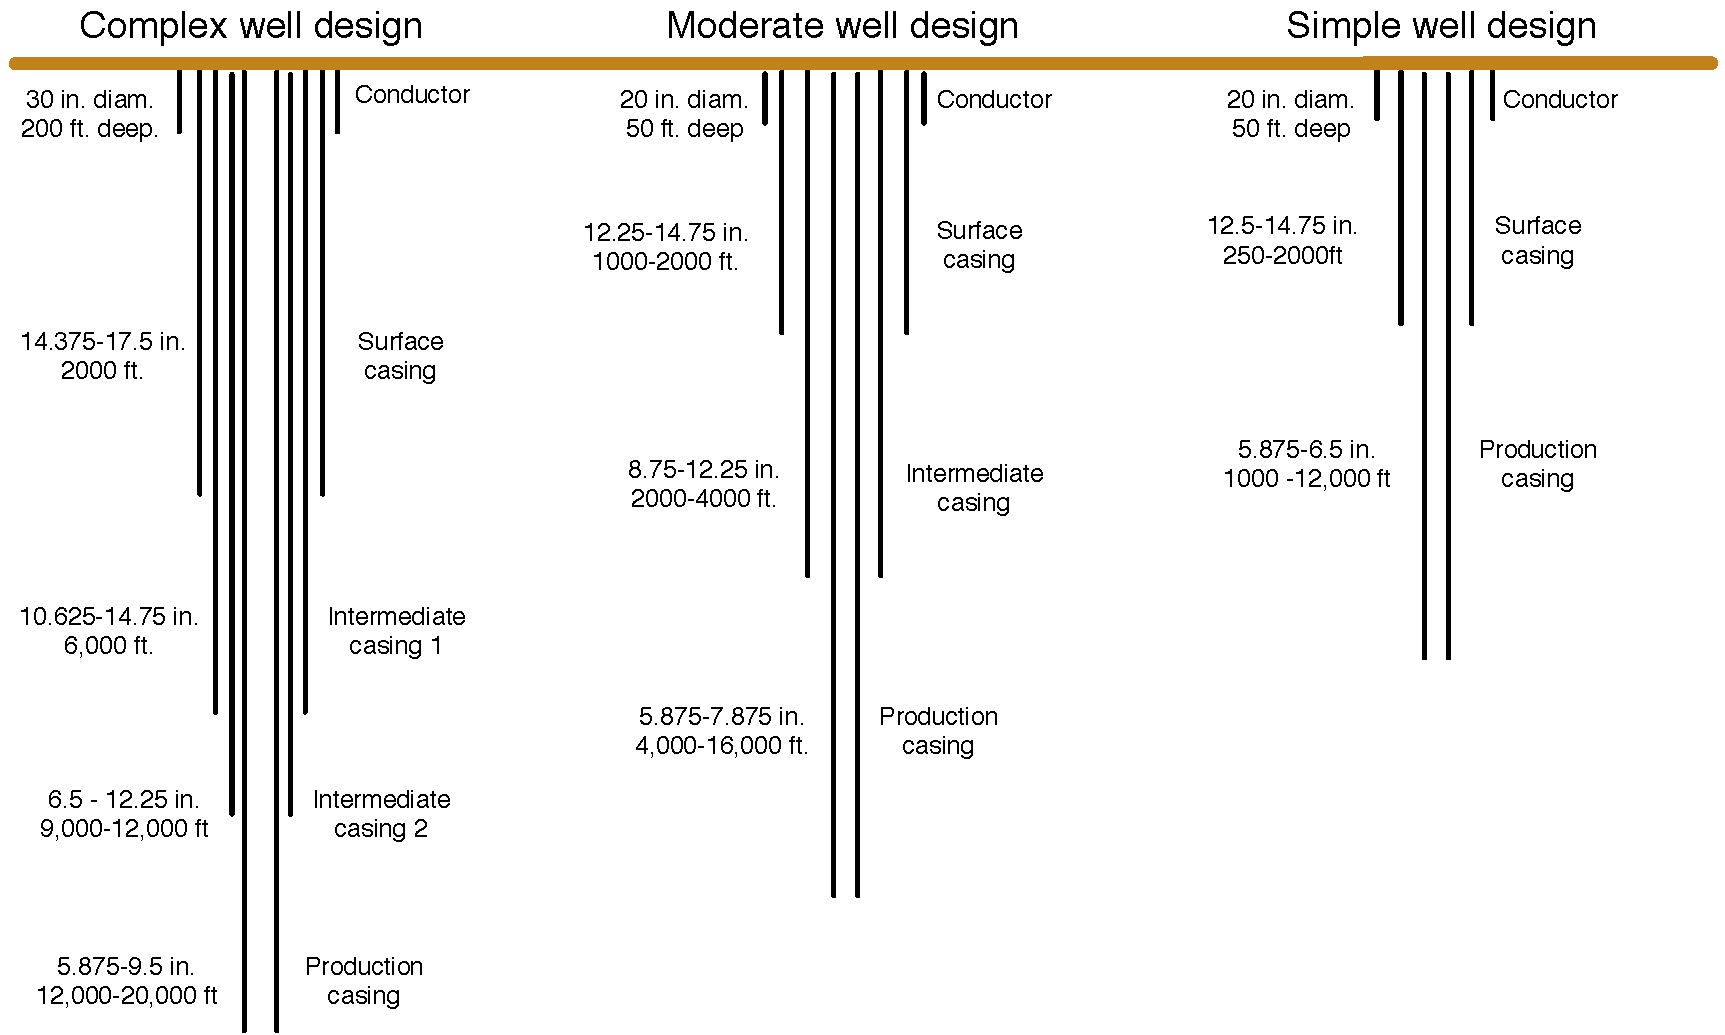
\includegraphics[width=1\columnwidth]{images/all_well_hole_diam.pdf}
\caption{Drilling hole diameters for simple, moderate and complex well construction.}
\label{fig:hole_diam}
\end{figure}

In addition, the energy efficiencies of rotary table/drill string torque provision and mud pump work can vary. The moderate efficiency settings for these terms are 45\% and 65\% respectively \cite{Vafi2016b}.  The low and high efficiency settings are 40\% and 50\% for the rotary table and 60\% and 70\% for the mud pumps, respectively.

The resulting energy consumption for rotary table and mud circulation uses are therefore modeled as:
\begin{equation}
E_{D} = E_{D}^{rt} + E_{D}^{mp} \quad\quad\eqnunit{mmBtu}
\end{equation}

where $E_{D}^{rt}$ is the energy consumed in rotary table work provision and $E_{D}^{mp}$ is the energy consumed in mud circulation pumps.

The energy consumption for rotary table work $E_{D}^{rt}$ is computed using the torque and torque factors as noted in GHGfrack documentation \cite{Vafi2016b}:
or,
\begin{equation}
E_{D}^{rt} = \frac{2 \pi T N}{33,000 \eta} \times t, \quad\quad\eqnunit{mmBtu}
\end{equation}

where $t$ is the amount of time that the rotary table is operating [h], $T$ is torque [ft-lb$_f$], $N$ is rotational speed [rpm], and $\eta$ is overall electro-mechanical efficiency of the rotary table drive system [-]. The value 33,000 is a unit conversion factor.  These values are set equal to \emph{GHGfrack} defaults in all results presented below. If the user wishes to change torque or other rotary table inputs, please use the \emph{GHGfrack} model directly. 

The energy consumption for mud circulation is computed using the overall pressure drop in the mud circulation system \cite{Vafi2016b}:
\begin{equation}
E_{D}^{mp} = \frac{\Delta p_{mp} Q}{1714 \eta} \times t, \quad\quad\eqnunit{mmBtu}
\end{equation}
where $\Delta p_{mp}$ is the pressure drop that must be overcome by the mud pump [psi], $Q$ is the mud flowrate [gal. per min.], $t$ is the time of mud pump operation [h] and 1714 is a conversion factor.

This pressure drop $\Delta p_{mp}$ is made up of a series of terms, including:
\begin{equation}
\Delta p_{mp} = \Delta p_{fric} + \Delta p_{dynamic} + \Delta p_{dm} - \Delta p_{hydrostatic} + \Delta p_{other} \quad\quad\eqnunit{psi}
\end{equation}
where subscripts refer to different pressure drop terms.  The $fric$ pressure drop is due to friction in drill string and annulus, modeled using a set of laminar and turbulent pipe and annulus flow models using different assumptions regarding non-Newtonian nature of drilling fluids (see \emph{GHGfrack} documentation \cite{Vafi2016a, Vafi2016b}).  The $dm$ term corresponds to energy imparted on the mud motor and converted to rotational motion of the bit.  In developing results for OPGEE, all \emph{GHGfrack} mud circulation settings are left at \emph{GHGfrack} defaults. If the user wishes to change mud circulation inputs, please use the \emph{GHGfrack} model directly. 

Given overall energy term $E_{D}$, we can compute fuel use in drilling as follows:
\begin{equation}
F_{D} = \frac{E_{D} \eta_{gs}}{LHV_{di}} \quad\quad\eqnunit{gal}
\end{equation}

where $F_{D}$ is the fuel use in drilling and development [gal], $\eta_{gs}$ is the efficiency of the drilling prime mover (diesel engine generator set) [-], and $LHV_{di}$ is the lower heating value of diesel fuel [mmBtu/gal].

A number of other \emph{GHGfrack} settings are required. For simplicity, in each model run, the drill pipe outer diameter (OD) [in] is set equal to 2.5 in. smaller than the smallest casing string inner diameter (ID).  In all cases, the drill pipe ID is set equal 0.5 in. smaller than the drill pipe OD.  The drill collar OD is set equal to 1.5 in.\, smaller than the smallest casing string ID.  The drill collar ID is set equal 0.5 in. smaller than the drill collar OD.  Also, in each well design, the last segment is set to an inclination angle of either 0$^\circ$ (vertical) or 90$^\circ$ (horizontal).  We do not apply a slanted transition zone (i.e., a 45 $^\circ$ zone).   

Given all of the above variables, a total of 816 \emph{GHGfrack} model runs are computed using an automated macro.  The resulting depths and fuel consumption quantities for all runs are illustrated in Figure \ref{fig:drilling1}.  

\begin{figure}[tb]
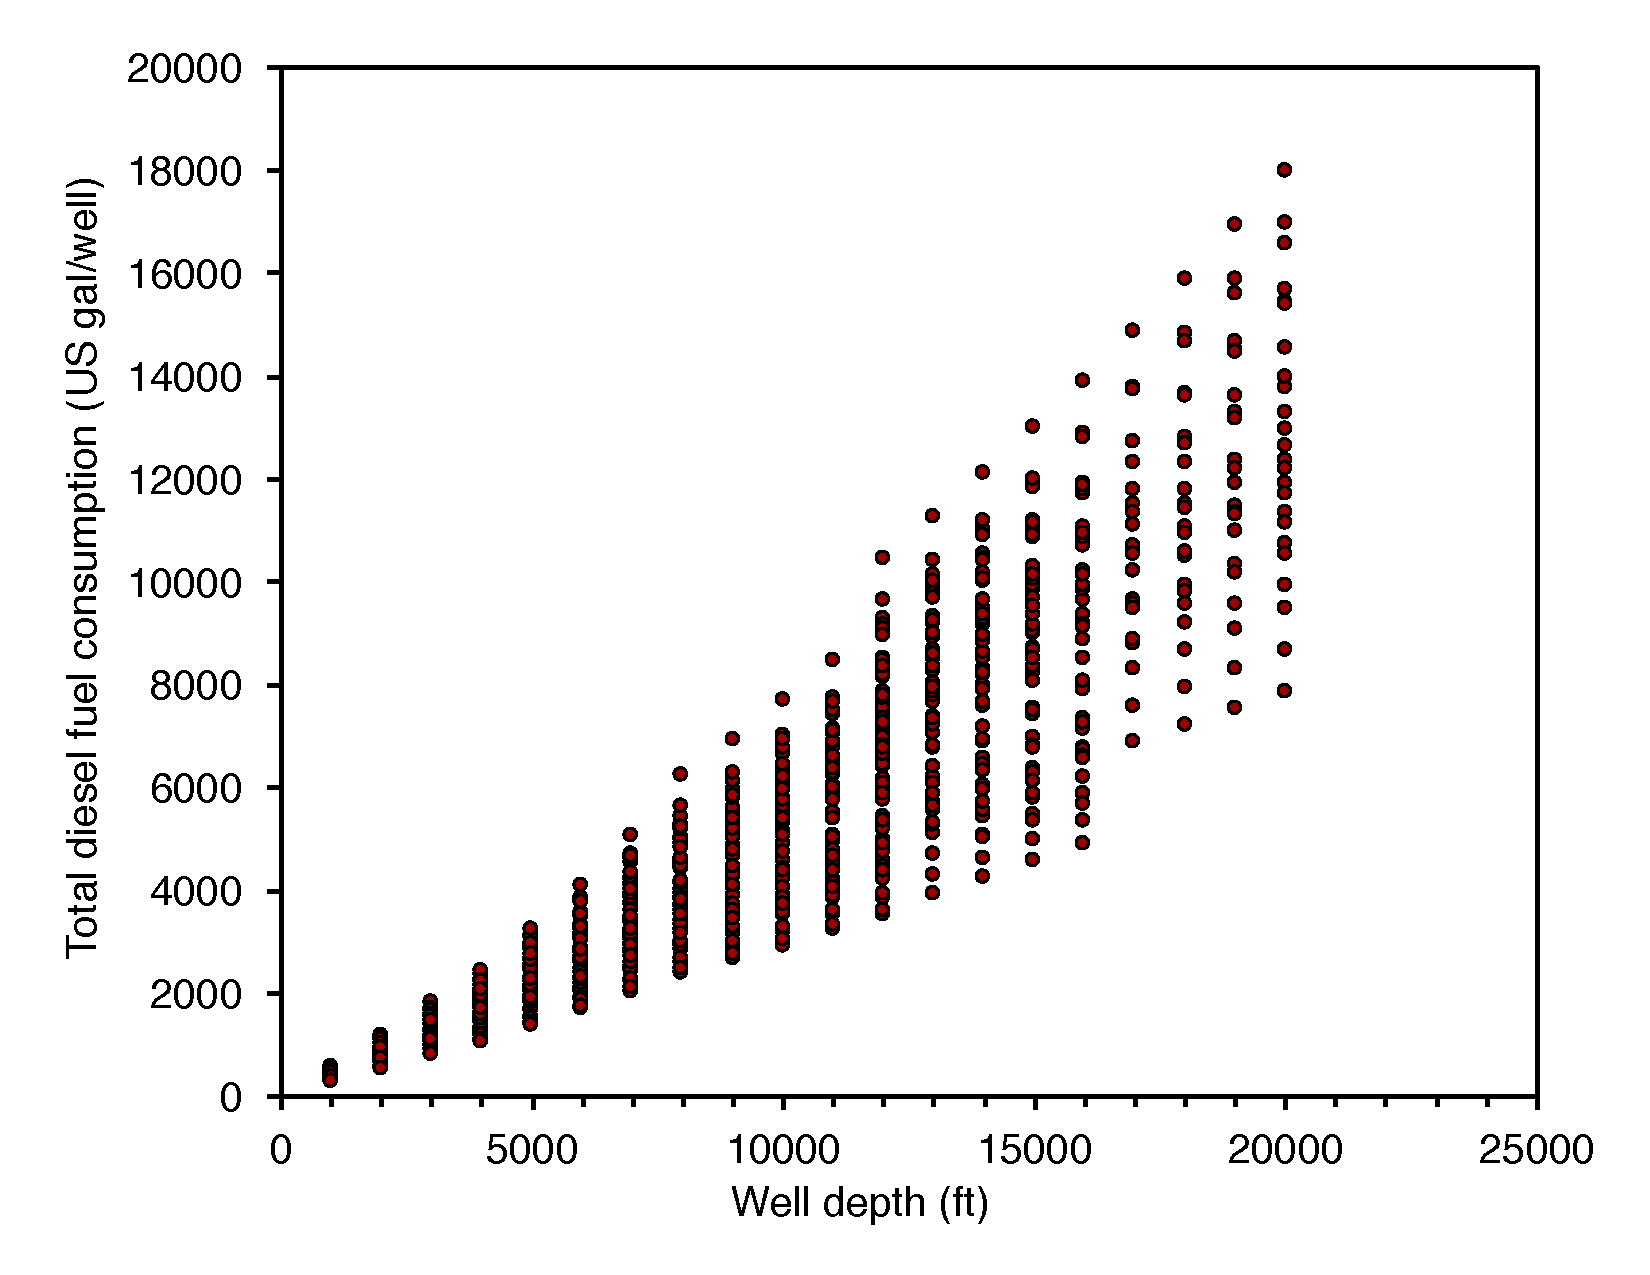
\includegraphics[width=0.8\columnwidth]{images/Drilling1.pdf}
\caption{All GHGfrack results for drilling fuel consumption in US gallons of diesel (includes both rotary table + mud circulation).}
\label{fig:drilling1}
\end{figure}

As can be seen, there is a wide range of energy consumption values for each depth.  To further understand drivers of emissions, we then segment these results into results from simple, moderate, and complex wells (Figure \ref{fig:drilling2}).

\begin{figure}[tb]
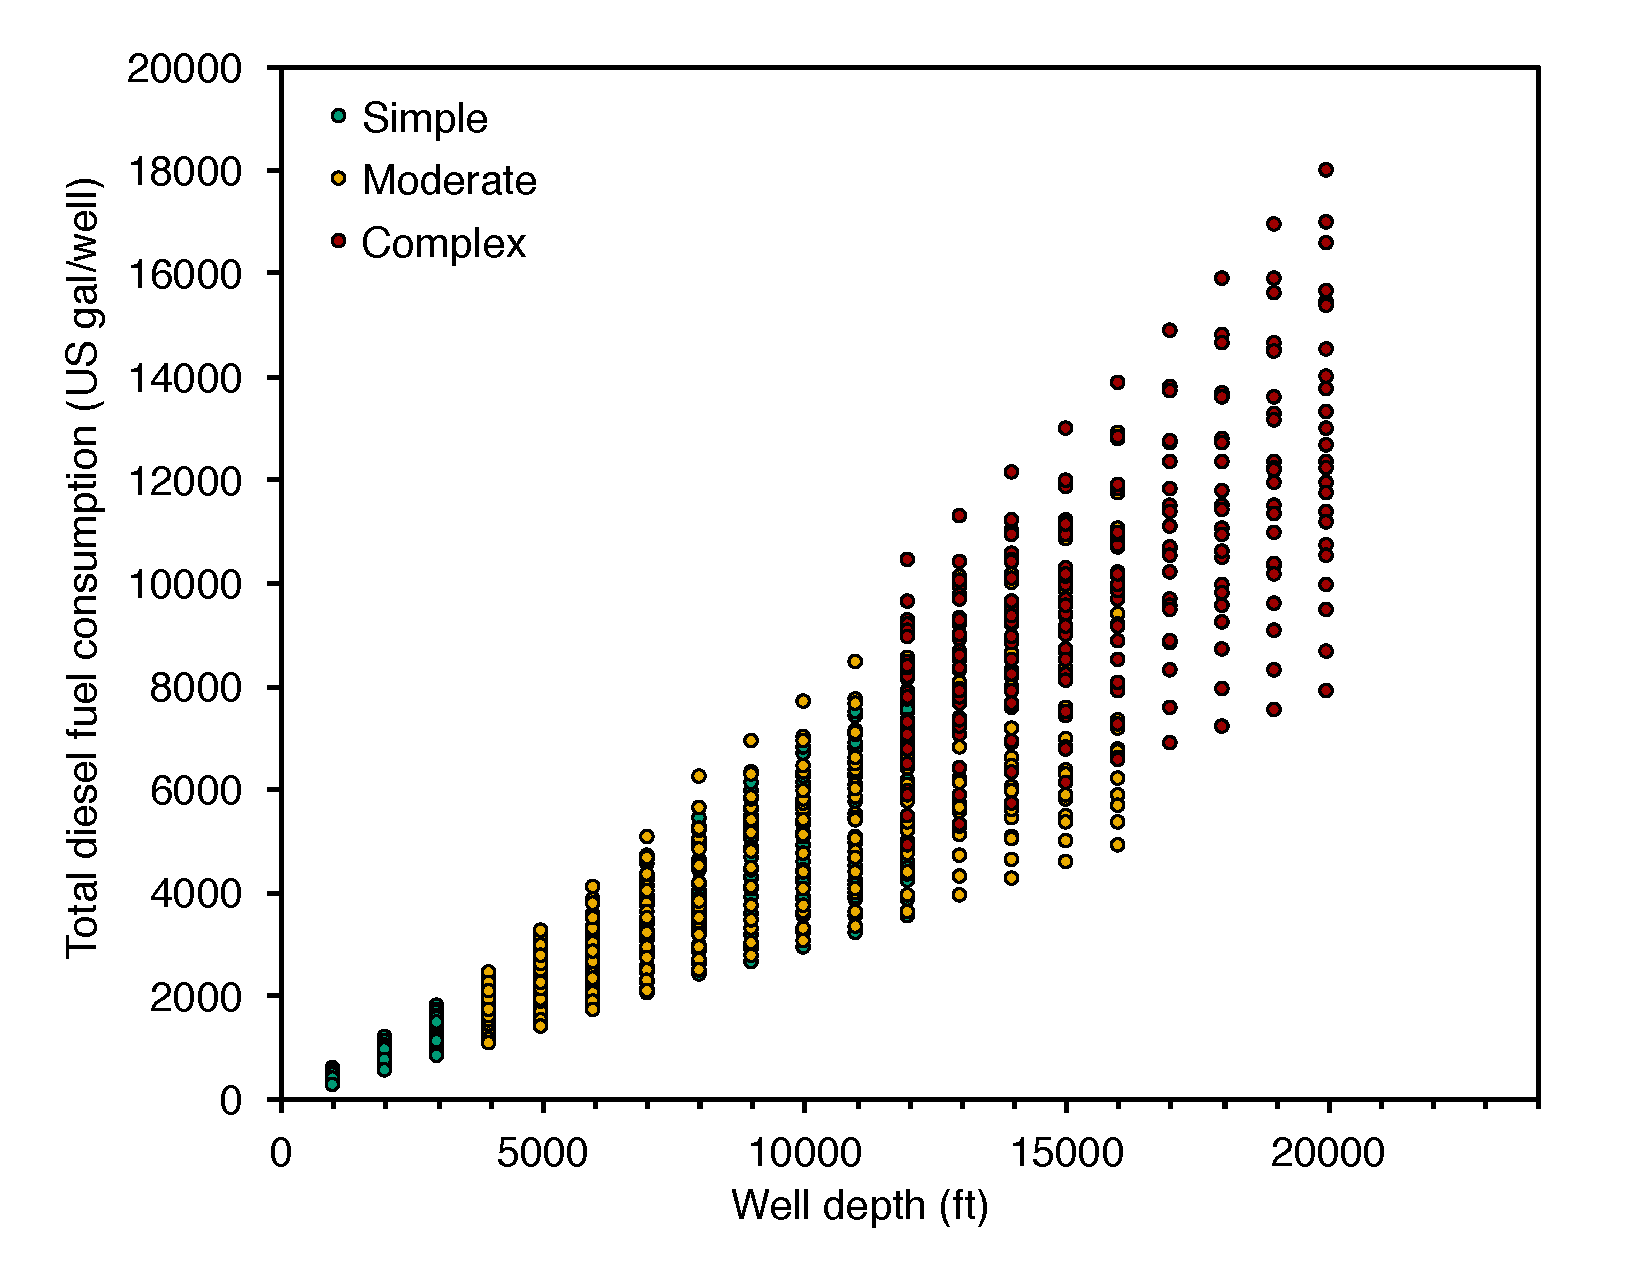
\includegraphics[width=0.8\columnwidth]{images/Drilling2.pdf}
\caption{GHGfrack results for drilling fuel consumption segmented by well complexity. Fuel consumption reported in US gallons of diesel (includes both rotary table + mud circulation).}
\label{fig:drilling2}
\end{figure}

We can further segment these results by separating vertical and horizontal wells and by noting the effect of rotary table and mud pump efficiency. This process is illustrated in Figure \ref{fig:drilling3} for the case of simple wells only.

\begin{figure}[tb]
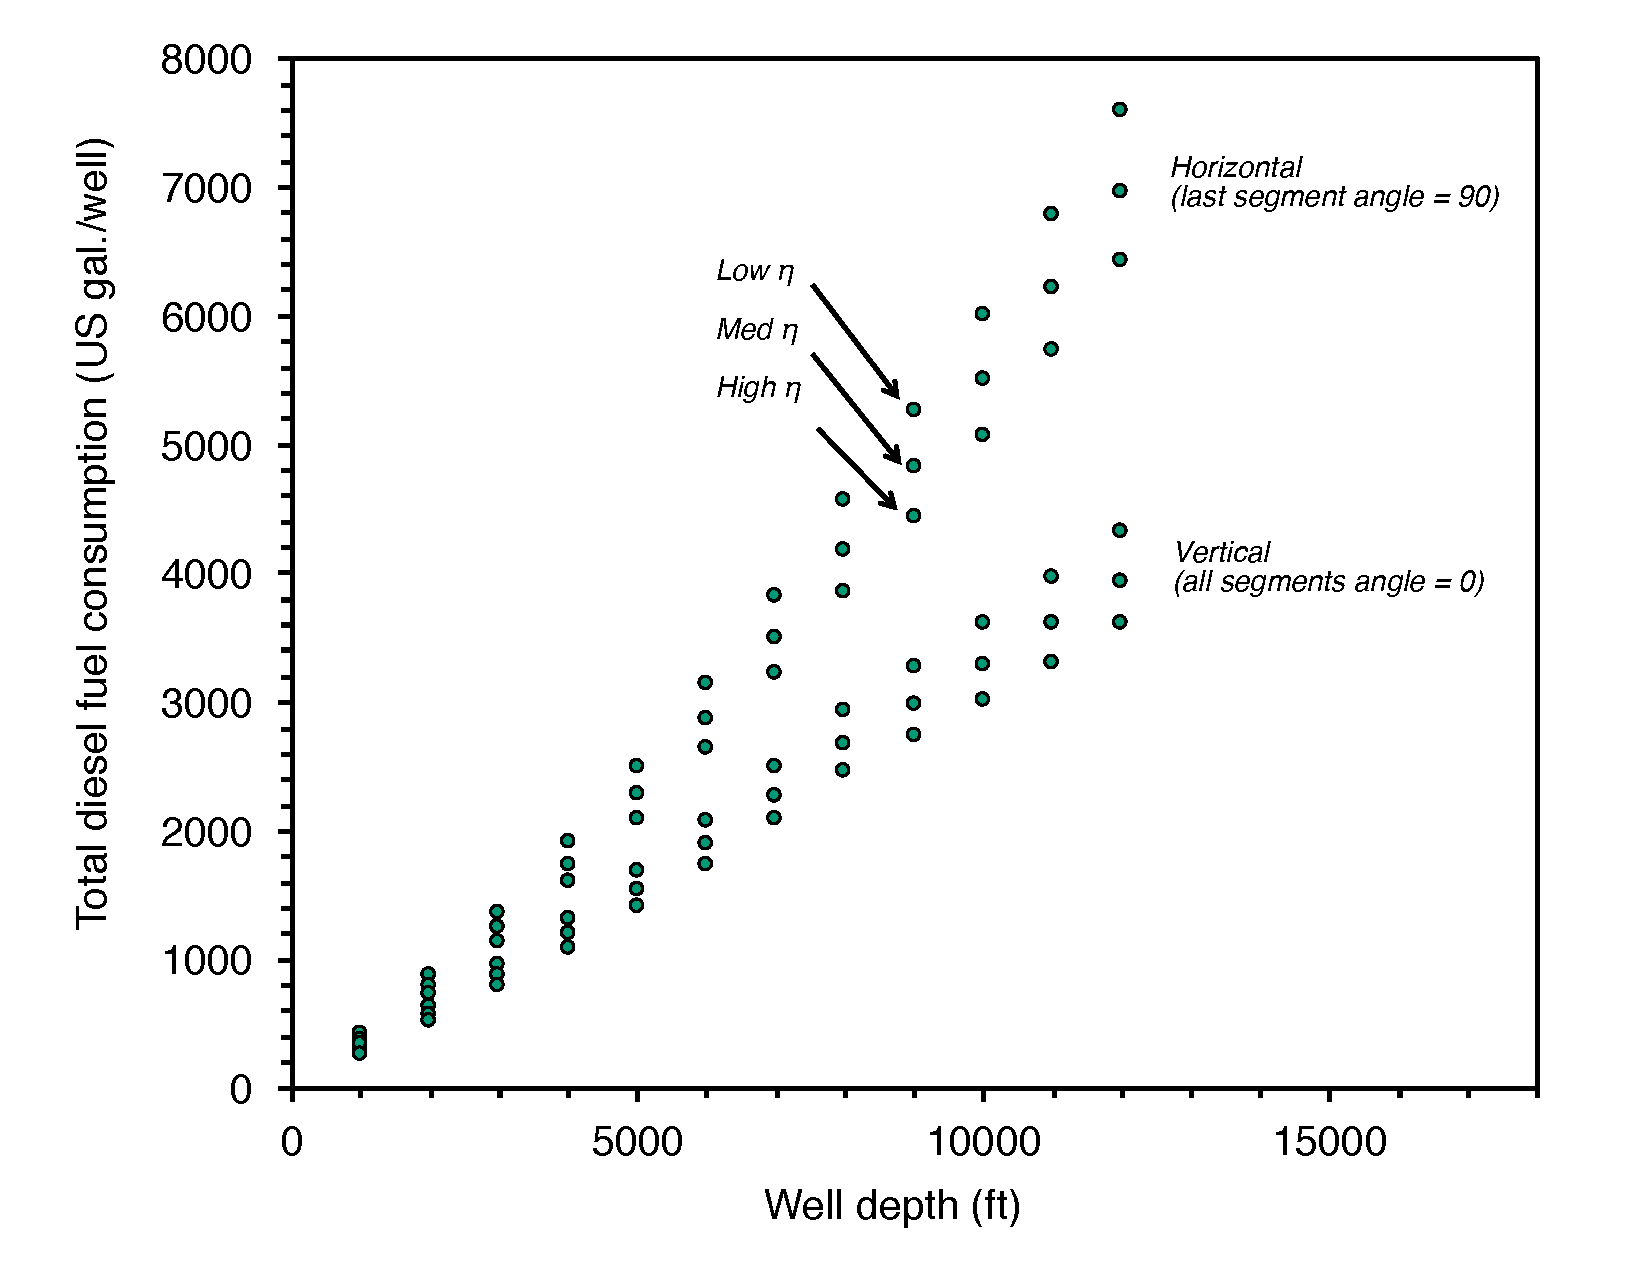
\includegraphics[width=0.8\columnwidth]{images/Drilling3.pdf}
\caption{GHGfrack results for drilling fuel consumption. Only simple wells are represented, and the results are segmented by efficiency and wellbore orientation. Fuel consumption reported in US gallons of diesel (includes both rotary table + mud circulation).}
\label{fig:drilling3}
\end{figure}

Using these segmented results, we construct a drilling intensity factor per-foot of drilled well for vertical wells.  Because the results in Figure \ref{fig:drilling3} are largely linear within a given efficiency setting and well geometry, we can use a linear model segmented by well category. Fuel intensity factors $FI$ [gal diesel fuel/ft.] are constructed separate for each ``line'' in Figure \ref{fig:drilling3} as follows: vertical wells are segmented by well-complexity, well diameter, and assumed efficiency setting.  A linear slope is computed to estimate the fuel intensity factor $FI$ by summing the total fuel use across all wells in a given well complexity-well size category and summing the total distance drilled across all wells in that category:
\begin{equation}
FI_{D}^{v,cat} = \frac{\sum_{i \in cat} F_{D}^{i}}{\sum_{i \in cat} D_{v}^{i}}
\quad\quad\eqnunitfrac{gal}{ft}
\end{equation}
where $i$ is the index for wells, $i \in cat$ represents the subset of all wells $i$ that are included in a given well-complexity, well diameter, and efficiency setting category.  $D_{v}^{i}$ is the vertical distance drilled (TVD) for each vertical well in the particular category.  These tabulated fuel intensity factors $I$ per foot of well drilled are included in OPGEE and selected using logic for each field depending on field well construction practices.

To compute the excess fuel required to drill horizontal wells, we compare each horizontal well to the vertical well of the same total drilling distance and compute the additional fuel use associated with making each well have a horizontal segment.  This additional fuel use can then be divided for each well by the length of the horizontal segment. This gives a horizontal well fuel intensity factor $FI$:
\begin{equation}
FI_{D}^{h,cat} = \frac{\sum_{i \in cat} \left(F_{D}^{i,h} - F_{D}^{i,v} \right)}{\sum_{i \in cat} D_{h}^{i}} \quad\quad\eqnunitfrac{gal}{ft}
\end{equation}

where $F_{D}^{i,h}$ is the fuel consumed in the horizontal version of well $i$ and $F_{D}^{i,v}$ is the fuel consumed in the vertical version of the same well $i$ [gal diesel].  The horizontal distance $D_{h}$ for a given well is the distance of the terminal well segment (horizontal).  This computation results in an incremental fuel consumption per ft. of horizontal well drilled [gal/ft. horizontal]. 

Using these two factors, we can compute the total fuel required to drill a horizontal or vertical well $i$ using a single expression:

% issue 19: everywhere we used D_w as field depth. Shouldn't we change D_v in eq. below?

\begin{minipage}{0.6\columnwidth}
\begin{fleqn}[0pt]
\begin{equation}
F_{D} =  D_{v}\left( FI_{D}^{v} \right)+ f_h D_{h} \left(FI_{D}^{v}+FI_{D}^{h}  \right) \quad\quad\eqnunitfrac{gallon diesel}{well}
\end{equation}
\end{fleqn}
\end{minipage}\hfill
\begin{minipage}{0.3\columnwidth}
        \begin{tabular}{|cl}
                        & \\
        $D_{v}$         & \xlname{Field\_depth}\\
        $FI_{D}^{v}$    & \xlname{Drilling\_fuel\_per\_foot\_vertical}\\
        $FI_{D}^{h}$    & \xlname{Drilling\_fuel\_per\_foot\_horizontal}\\
        $f_{h}$         & \xlname{Fraction\_wells\_horizontal}\\
        $D_{h}$         & \xlname{Length\_lateral}\\
                         & \\
        \end{tabular}
\end{minipage}
where $f_h$ is the fraction of wells [0-1] with horizontal segment of length $D_h$ [ft].

The total energy to drill the wells in the field is then:

\begin{minipage}{0.6\columnwidth}
\begin{fleqn}[0pt]
\begin{equation}
F_{F} =  F_{D} N_{w,tot} LHV_{di} \quad\quad\eqnunitfrac{mmBtu}{field}
\end{equation}
\end{fleqn}
\end{minipage}\hfill
\begin{minipage}{0.3\columnwidth}
        \begin{tabular}{|cl}
                        & \\
        $LHV_{di}$      & \xlname{LHV\_diesel}\\
                        & \\
        \end{tabular}
\end{minipage}

The energy intensity of drilling per unit of energy produced is therefore calculated as follows:
%%%%%%%%%%
\begin{equation}
ei_{D} = \frac{F_{F}}{E_{o,F}} \quad\quad\eqnunit{-}
\end{equation}
%%%%%%%%%%

The energy intensity of drilling tends to be small when amortized over total well productivity, with values on order 10$^{-6}$ to 10$^{-2}$ mmBtu consumed in drilling per mmBtu produced over the life of the well (i.e., 1 part in 100 to 1 part in 1 million).

\subsubsection{Emissions from hydraulic fracturing}

The practice of hydraulic fracturing can consume large amounts of energy. This is because modern high-volume multi-stage hydraulic fracturing requires injecting large amounts of fluid at high pressures. \emph{GHGfrack} models the injection of hydraulic fracturing fluids by accounting for the pressure required for fracturing:
\begin{equation}
\Delta p_{hf} = \Delta p_{fracture} + \Delta p_{fric} - \Delta p_{hydrostatic}  \quad\quad\eqnunit{psi} 
\end{equation}

where $\Delta p_{fracture}$ is the fracturing pressure required to overcome the fracturing gradient [psi], $ \Delta p_{fric}$ is the frictional pressure drop during injection [psi], and $\Delta p_{hydrostatic}$ is the contribution from the hydrostatic head of water in the wellbore [psi].

As in the case of mud pump injection energy, the energy requirements of hydraulic fracturing are calculated from the pressure drop as follows:
\begin{equation}
E_{D}^{hf} = \frac{\Delta p_{hf} Q_{hf}}{1714 \eta} \times t \quad\quad\eqnunit{mmBtu} 
\end{equation}
and the fuel consumption due to hydraulic fracturing is computed similarly to the fuel consumption due to drilling:
\begin{equation}
F_{D}^{hf} = \frac{E_{D}^{hf} \eta_{gs}}{LHV_{di}} \quad\quad\eqnunit{gal}
\end{equation}

We compute the fuel consumption due to hydraulic fracturing using \emph{GHGfrack} for numerous cases and use the results to create simple correlations for use in OPGEE.  We use a number of default \emph{GHGfrack} assumptions during the runs, including:
\begin{itemize}
\item Injection string ID = 5 in.
\item Horizontal lateral length = 5000 ft.
\item Fracturing fluid density = 9.0 lbm/gal.
\item Viscosity = 1 cp
\item Pipe roughness = 0.00008 in
\item Length of fracturing stage = 300 ft
\item Number of computational segments = 10
\item Pump efficiency = 65\%
\item Injection time = 48 hr
\end{itemize}
In order to generate the relationships used in OPGEE, we vary two key inputs to the \emph{GHGfrack} hydraulic fracturing module: (1) amount of fracturing fluid injected, and (2) fracturing gradient.  In these runs, the fracturing gradient is varied from 0.6 psi/ft to 1.0 psi/ft in increments of 0.05 psi/ft.  Also, in these runs the amount of fluid injected is varied from 1 to 5 $\times 10^6$ gallons in increments of 1$\times 10^6$ gallons.  Therefore, a total of 45 \emph{GHGfrack} fracturing simulations are performed.

The results from these \emph{GHGfrack} simulations are shown in Figure \ref{fig:fracturing1}.  We fit quadratic functions to each set of results from the same fracturing gradient value.  In each case, the R$^2$ value is $\geq$0.999.  The resulting quadratic function coefficients are used in OPGEE to predict hydraulic fracturing energy use in a particular field based on the volume of fracturing fluid injected.  The equation used is:

\begin{minipage}{0.6\columnwidth}
\begin{fleqn}[0pt]
\begin{equation}
F_{D}^{hf}=  a V_{hf}^2 + b V_{hf} + c \eqnunitfrac{gal. diesel}{well}
\end{equation}
\end{fleqn}
\end{minipage}\hfill
\begin{minipage}{0.3\columnwidth}
        \begin{tabular}{|cl}
                        & \\
        $F_{D}^{hf}$      & \xlname{Fracturing\_fuel\_per\_well}\\
        $V_{hf}$        & \xlname{Volume\_per\_well\_fractured}\\
                        & \\
        \end{tabular}
\end{minipage}

where $a$, $b$ and $c$ are fitting constants unique to each fracturing gradient.  The results for the fitting constants $a$, $b$ and $c$ are shown in Table \ref{tab:fracturing_fit}.

\begin{table}
\begin{scriptsize}
\tablefirsthead{\toprule Fracturing gradient [psi/ft]  & $a$ & $b$ & $c$        \\
\midrule}
\tablehead{}
\tabletail{}
\tablelasttail{\bottomrule}
\tablecaption{Constants for quadratic fit of fracturing fuel consumption equation}
\label{tab:fracturing_fit}
\begin{threeparttable}
\begin{supertabular*}{0.6\columnwidth}{p{0.12\columnwidth}p{0.12\columnwidth}p{0.12\columnwidth}p{0.12\columnwidth}}
0.60 & 588.55 & -488.77 & 1184.50 \\
0.65 & 599.49 & -246.27 & 1349.20 \\
0.70 & 511.30 & 575.63  & 964.32  \\
0.75 & 499.47 & 924.06  & 1012.50 \\
0.80 & 566.77 & 1090.40 & 1101.60 \\
0.85 & 570.18 & 1378.20 & 1162.60 \\
0.90 & 523.67 & 1882.70 & 1233.90 \\
0.95 & 664.49 & 1512.60 & 1922.70 \\
1.00 & 477.57 & 3025.40 & 752.02 \\
\end{supertabular*}
\end{threeparttable}
\end{scriptsize}
\end{table}

\begin{figure}[tb]
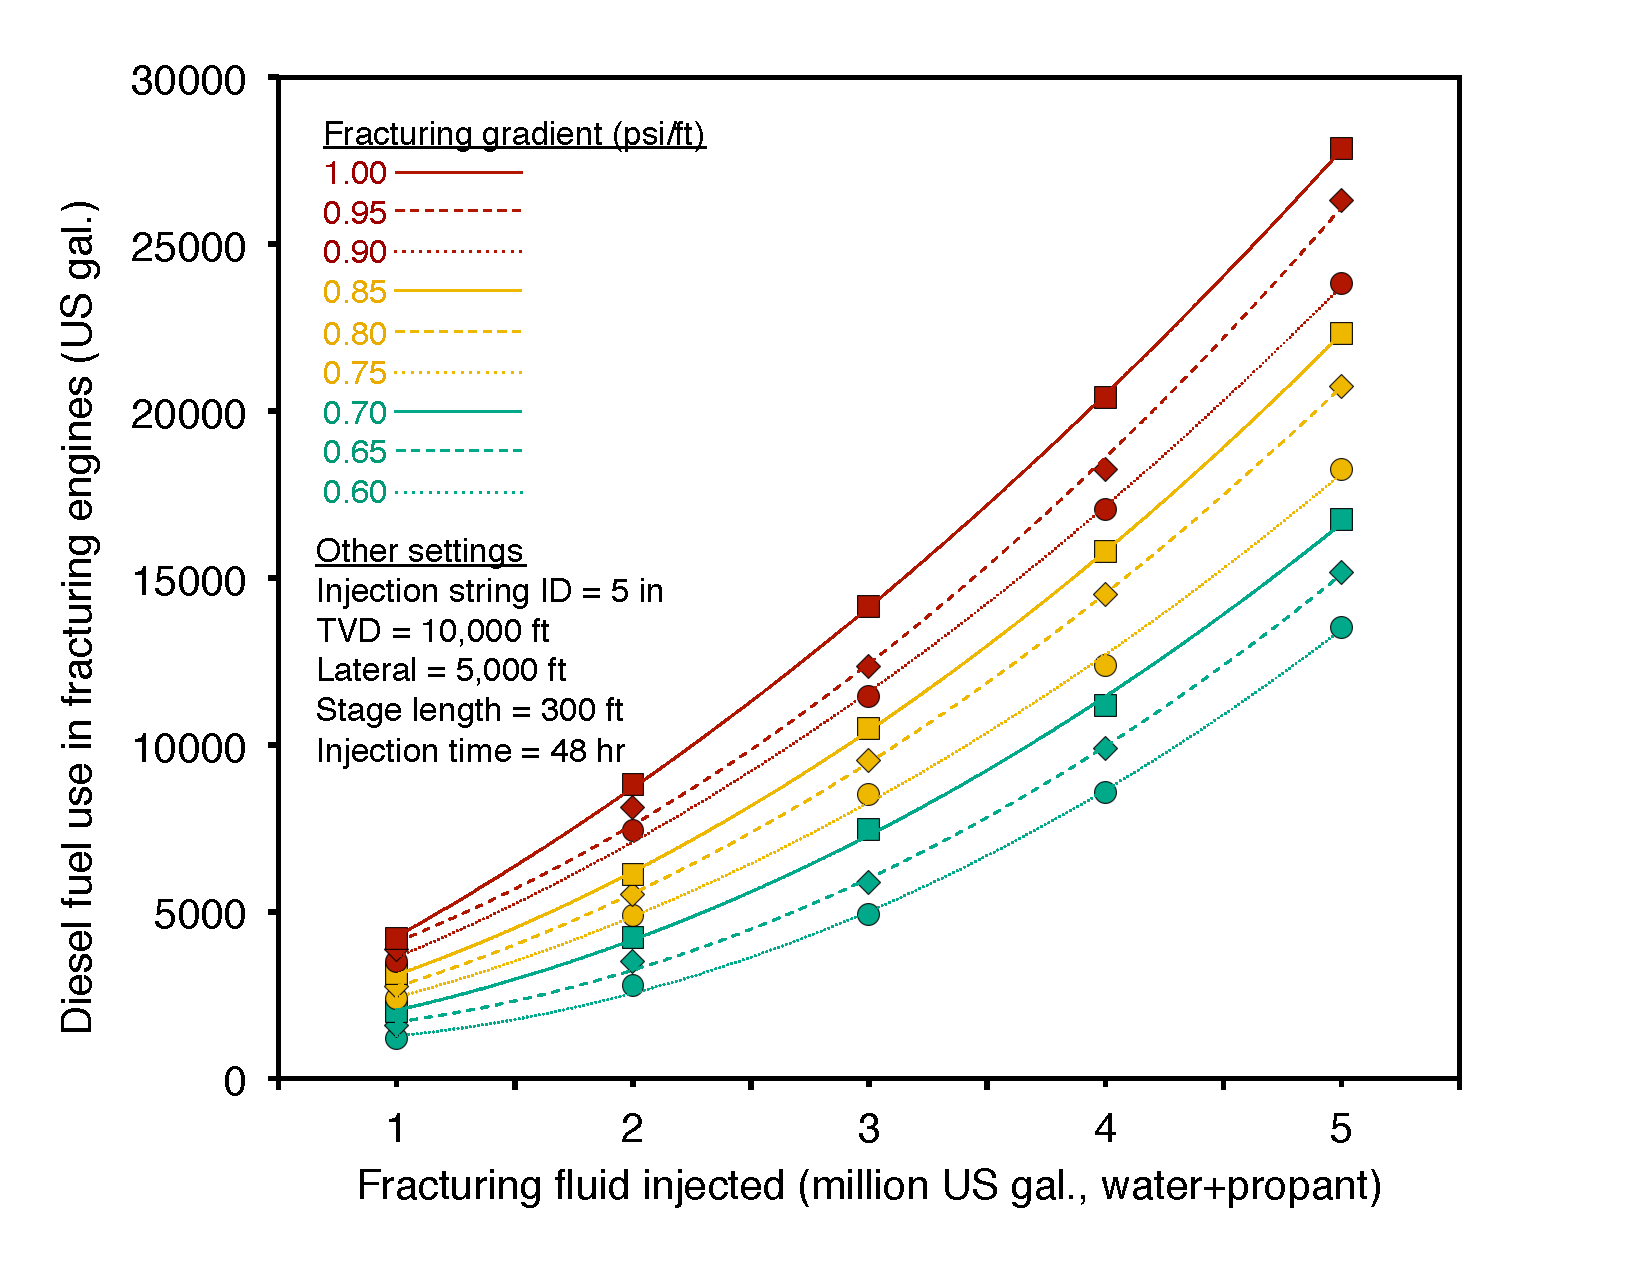
\includegraphics[width=0.8\columnwidth]{images/Fracturing1.pdf}
\caption{Fuel use in hydraulic fracturing as a function of fracturing volume. Each curve represents a different fracturing gradient value, ranging from 0.6 psi/ft to 1.0 psi/ft.}
\label{fig:fracturing1}
\end{figure}

\subsubsection{Emissions from land use impacts}

Land use impacts during drilling and field development are included in OPGEE for three categories: soil carbon that is oxidized upon disturbance of land, biomass carbon that is oxidized due to biomass disturbance, and emissions from foregone sequestration, due to the fact that biomass carbon sequestration is slowed on cleared land. For each of these impacts, emissions estimates from Yeh et al. \cite{Yeh2010} are included. Yeh et al. measured impacts over a 150 year period, which is not in alignment with other analyses that use 30 year land use impact calculations. For this reason, calculations from Yeh et al. were modified to reduce the timeframe for analysis to 30 years, reducing the amount of regrowth possible \cite{Yeh2012}. 

The user has the option to choose a 30 year or 150 year analysis timeframe using the \xlname{Timeframe\_land\_use} secondary input. The default analysis timeframe is set to 30 years.

In order to estimate land use GHG emissions, three settings are required as primary inputs. First, the crude production method must be chosen. The options for crude production method include conventional production via wellbore (primary, secondary, and tertiary recovery of conventional and heavy hydrocarbons, including in situ recovery of bitumen) and mining-based production of bitumen. This is computed using the \xlname{Oil\_sands\_mine\_int\_01} and \xlname{Oil\_sands\_mine\_nonint\_01} primary inputs (if either is 1, then production is mining-based, otherwise well-based).

Next, the carbon richness of the ecosystem is specified. Options include low, moderate, and high carbon richness. Low carbon richness estimates are derived from California production in the semi-arid to arid central valley of California \cite{Yeh2010}. The high carbon richness estimates are derived from forested regions in Alberta (e.g., rocky mountain foothills) \cite{Yeh2010}. Moderate carbon richness is considered a mixed ecosystem with carbon richness between these ecosystems. The carbon richness of the ecosystem is set with the \xlname{Low\_ecosystem\_richness\_01}, \xlname{Med\_ecosystem\_richness\_01}, and \xlname{High\_ecosystem\_richness\_01} primary inputs.

Lastly, the intensity of field development must be specified. High intensity field development corresponds to high fractional disturbance, such as in a field drilled on tight spacing. Low intensity field development corresponds to a sparsely developed field with little fractional disturbance. Moderate field development occurs between these two extremes. Work by Yeh et al. \cite{Yeh2010} can be consulted for satellite images of low and high field development intensity. The intensity of land disturbance is set with the \xlname{Low\_land\_disturbance\_01}, \xlname{Med\_land\_disturbance\_01}, and \xlname{High\_land\_disturbance\_01} primary inputs.

Emissions associated with each choice are shown in Table \ref{tab:default_land_use_emissions_30} and \ref{tab:default_land_use_emissions_150}  in units of gCO$_2$eq GHGs per MJ of crude oil produced. These values are looked up for use in the calculation. The two tables are for different time periods of analysis from Yeh et al. \cite{Yeh2010}, 30 years and 150 years. A 30 year analysis is roughly the length of an industrial project and accounts for reassimilation of carbon during the project life. A 150 year analysis extends this and includes reassimilation that occurs after the project ends. 


\subsubsection{Flowback emissions and venting during drilling \& development}

Completions and workover events can result in flowback emissions. Flowback occurs after the completion event when the well is opened to the production system, often at low pressure, to allow any material (i.e., excess fracturing water) to flow to the surface. Gas produced during flowback can be captured for use (so-called reduced emissions completion, or REC), flared, or vented. The two secondary inputs controlling emissions per completions event are \xlname{Flaring\_Fracturing\_Flowback} and \xlname{REC\_Fracturing\_Flowback}. If these are equal to 1, then the appropriate technologies, flaring or REC is applied. Similarly, these secondary inputs control whether emissions during workover flowback events are controlled with flaring, with REC, with both flaring and REC, or with neither.

% issue 7: which section is referred in above paragraph?

Once these emissions are estimated, they are combined with the number of wells drilled and wells worked over using. The total number of events is equal to the total number of wells \xlname{Num\_prod\_wells}+\xlname{Num\_water\_inj\_wells} times the number of events per well. Completions are only assumed to occur once per well and workovers are assumed to be performed \xlname{Number\_well\_workovers} per well.

\subsection{Defaults for drilling \& development}

Default values for drilling \& development calculations are shown in Tables \ref{tab:default_land_use_emissions_30},\ref{tab:default_land_use_emissions_150}, \ref{tab:primary_inputs_drilling}, and \ref{tab:secondary_inputs_drilling}. 

\begin{table}
\begin{scriptsize}
\caption{Land use GHG emissions for 30 year analysis period from field drilling and development in OPGEE for conventional oil operations [gCO$_2$eq/MJ of crude oil produced]. Data from Yeh et al \cite{Yeh2010}.}
\label{tab:default_land_use_emissions_30}
\begin{tabular}{p{0.13\columnwidth}p{0.06\columnwidth}p{0.06\columnwidth}p{0.06\columnwidth}p{0.06\columnwidth}p{0.06\columnwidth}p{0.06\columnwidth}p{0.06\columnwidth}p{0.06\columnwidth}p{0.06\columnwidth}}
\toprule
& \multicolumn{3}{p{0.25\columnwidth}}{Low carbon stock } & \multicolumn{3}{p{0.25\columnwidth}}{Moderate carbon stock } & \multicolumn{3}{p{0.25\columnwidth}}{High carbon stock}\\
& \multicolumn{3}{p{0.25\columnwidth}}{(semi-arid grasslands)} & \multicolumn{3}{p{0.25\columnwidth}}{(mixed)} & \multicolumn{3}{p{0.25\columnwidth}}{(forested)}\\
\cmidrule{2-4} \cmidrule{5-7} \cmidrule{8-10}
& Low int. & Med. int. & High int. & Low int. & Med. int. & High int. & Low int. & Med. int. & High int.\\
\midrule
Soil carbon & 0.03 & 0.13 & 0.35 & 0.22 & 0.57 & 1.93 & 0.40 & 1.01 & 3.51\\
Biomass & 0.00 & 0.00 & 0.00 & 0.34 & 0.68 & 1.47 & 0.68 & 1.36 & 2.94\\
Foregone seq.\ & 0.00 & 0.00 & 0.00 & 0.01 & 0.01 & 0.01 & 0.01 & 0.01 & 0.02\\
\bottomrule
\end{tabular}
\end{scriptsize}
\end{table}


\begin{table}
\begin{scriptsize}
\caption{Land use GHG emissions for 150 year analysis period from field drilling and development in OPGEE for conventional oil operations [gCO$_2$eq/MJ of crude oil produced]. Data from Yeh et al \cite{Yeh2010}.}
\label{tab:default_land_use_emissions_150}
\begin{tabular}{p{0.13\columnwidth}p{0.06\columnwidth}p{0.06\columnwidth}p{0.06\columnwidth}p{0.06\columnwidth}p{0.06\columnwidth}p{0.06\columnwidth}p{0.06\columnwidth}p{0.06\columnwidth}p{0.06\columnwidth}}
\toprule
& \multicolumn{3}{p{0.25\columnwidth}}{Low carbon stock } & \multicolumn{3}{p{0.25\columnwidth}}{Moderate carbon stock } & \multicolumn{3}{p{0.25\columnwidth}}{High carbon stock}\\
& \multicolumn{3}{p{0.25\columnwidth}}{(semi-arid grasslands)} & \multicolumn{3}{p{0.25\columnwidth}}{(mixed)} & \multicolumn{3}{p{0.25\columnwidth}}{(forested)}\\
\cmidrule{2-4} \cmidrule{5-7} \cmidrule{8-10}
& Low int. & Med. int. & High int. & Low int. & Med. int. & High int. & Low int. & Med. int. & High int.\\
\midrule
Soil carbon & 0.03 & 0.13 & 0.35 & 0.10 & 0.35 & 1.50 & 0.16 & 0.57 & 2.65\\
Biomass & 0.00 & 0.00 & 0.00 & 0.01 & 0.09 & 0.33 & 0.02 & 0.17 & 0.65\\
Foregone seq.\ & 0.00 & 0.00 & 0.00 & 0.02 & 0.03 & 0.05 & 0.03 & 0.05 & 0.09\\
\bottomrule
\end{tabular}
\end{scriptsize}
\end{table}

\begin{landscape}

\begin{tiny}
\tablefirsthead{\toprule Param. & Description & Defined name & Default & Literature range & Unit & Sources & Notes\\
\midrule}
\tablehead{ \multicolumn{8}{p{1\columnwidth}}{\textit{Continued from previous page}}\\ \toprule Param. &Description & Defined name &Default & Literature range & Unit & Sources & Notes \\ 
\midrule }
\tabletail{\bottomrule \multicolumn{8}{p{1\columnwidth}}{\textit{Continued on next page...}}\\}
\tablelasttail{\bottomrule}
\tablecaption{Primary inputs used in \sheet{Drilling \& Development} sheet.}
\label{tab:primary_inputs_drilling}
\begin{threeparttable}
\begin{supertabular*}{1\columnwidth}{p{0.03\columnwidth}p{0.25\columnwidth}p{0.25\columnwidth}p{0.07\columnwidth}p{0.07\columnwidth}p{0.07\columnwidth}p{0.07\columnwidth}p{0.07\columnwidth}}
$D_{w}$ 	    & Vertical depth of wells			    & \xlname{Field\_depth}  & 7240 		& 100-20,000 	&[ft] &  & \\ 
$n_{wo}$ 		& Number of production wells			& \xlname{Num\_prod\_wells} & 8 		& 1-10,000 & [Wells] 	&  &  \\
$n_{wi}$ 		& Number of injector wells		    	& \xlname{Num\_water\_inj\_wells} & 5 		& 0-1000 & [Wells] 	&  &  \\
$y_{OS,mi}$     & Oil sands mine integrated with upgrader?  & \xlname{Oil\_sands\_mine\_int\_01} & 0 & 0-1 & [binary 0-1] & & \\
$y_{OS,mn}$     & Oil sands mine non-integrated with upgrader?  & \xlname{Oil\_sands\_mine\_nonint\_01} & 0 & 0-1 & [binary 0-1] & & \\
$y_{ER,l}$     & Low carbon richness (semi-arid grasslands)  & \xlname{Low\_ecosystem\_richness\_01} & 0 & 0-1 & [binary 0-1] & & \\
$y_{ER,m}$     & Moderate carbon richness (mixed)  & \xlname{Med\_ecosystem\_richness\_01} & 0 & 0-1 & [binary 0-1] & & \\
$y_{ER,h}$     & High carbon richness (forested)  & \xlname{High\_ecosystem\_richness\_01} & 0 & 0-1 & [binary 0-1] & & \\
$y_{DO,l}$     & Low intensity development and low oxidation  & \xlname{Low\_land\_disturbance\_01} & 0 & 0-1 & [binary 0-1] & & \\
$y_{DO,m}$     & Moderate intensity development and moderate oxidation  & \xlname{Med\_land\_disturbance\_01} & 0 & 0-1 & [binary 0-1] & & \\
$y_{DO,h}$     & High intensity development and High oxidation  & \xlname{High\_land\_disturbance\_01} & 0 & 0-1 & [binary 0-1] & & \\
\end{supertabular*}
%\begin{tablenotes}
%\item[a] Insert text of note here
%\end{tablenotes}
\end{threeparttable}
\end{tiny}

\newpage

\begin{tiny}
\tablefirsthead{\toprule Param. & Description & Defined name & Default & Literature range & Unit & Sources & Notes\\
\midrule}
\tablehead{ \multicolumn{8}{p{1\columnwidth}}{\textit{Continued from previous page}}\\ \toprule Param. &Description & Defined name &Default & Literature range & Unit & Sources & Notes \\ 
\midrule }
\tabletail{\bottomrule \multicolumn{8}{p{1\columnwidth}}{\textit{Continued on next page...}}\\}
\tablelasttail{\bottomrule}
\tablecaption{Secondary inputs used in \sheet{Drilling \& Development} sheet.}
\label{tab:secondary_inputs_drilling}
\begin{threeparttable}
\begin{supertabular*}{1\columnwidth}{p{0.03\columnwidth}p{0.25\columnwidth}p{0.25\columnwidth}p{0.07\columnwidth}p{0.07\columnwidth}p{0.09\columnwidth}p{0.07\columnwidth}p{0.07\columnwidth}}
$C_{w}$        & Well complexity                                & \xlname{Well\_complexity} & Moderate & Simple-Complex & [-] & \cite{Vafi2016b} & \\
$L_{w,h}$ 	    & Length of horizontal segment of well (lateral) & \xlname{Length\_lateral} & 5000 	& 1000-10,000 	&[ft] &  & a\\ 
$I_{f,D}^{h} $ 	& Horizontal drilling incremental fuel intensity	& - &0.380 	& 0.218 - 0.459 & [gal/ft. horizontal] & \cite{Vafi2016b} & b \\
$I_{f,D}^{v} $ 	& Vertical drilling fuel intensity			 	& - &0.404 	& 0.226 - 0.724 & [gal/ft.] & \cite{Vafi2016b} & b \\
$f_L$		    & Fraction of wells with horizontal segment		& \xlname{Fraction\_wells\_horizontal} & 0		& 0 - 1		& [fraction horizontal] & & \\
$f_f$		    & Fraction of wells fractured                   & \xlname{Fraction\_wells\_fractured} & 0		& 0 - 1		& [fraction fractured] & & \\
$n_{wo}$        & Workovers needed over lifetime of well        & \xlname{Number\_well\_workovers} & 4 & 0-10 & [workovers] & & \\
$p_f$           & Fracturing pressure gradient (rock strength)  & \xlname{Pressure\_gradient\_fracturing}   & 0.7 & 0.6-1 & [psi/ft] & & \\
$P_{wo}$        & Oil field productivity category               & \xlname{Well\_productivity\_crude\_oil} & Med & Low-High  & & \\
$P_{wg}$        & Natural gas field productivity category       & \xlname{Well\_productivity\_natural\_gas} & Med & Low-High  & & \\
$S_{w} $        & Hole size                                     & \xlname{Well\_size}       & Med       & Small-Large   & [-] & \cite{Vafi2016b} & \\
$T_{lu}$        & Timeframe of landuse analysis                 & \xlname{Timeframe\_land\_use} & 30 & 30-150   & [y] & \cite{Yeh2010} & \\
$V_f$           & Fracturing fluid injection volume             & \xlname{Volume\_per\_well\_fractured} & 3 & 1-8 & [M gallons/well] & & \\
$y_{f,f}$       & Fracturing flowback flared?                      & \xlname{Flaring\_fracturing\_flowback} & 0    &0/1    &[binary 0-1] & & \\
$y_{f,rec}$     & Fracturing flowback captured with reduced emissions completions?  & \xlname{REC\_fracturing\_flowback} & 1 & 0-1 & [binary 0-1] & & \\
$\eta_{rig}$    & Rig efficiency                                & \xlname{eta\_rig} &   Med & Low-High  & [\%] & \cite{Vafi2016b} & a \\
\end{supertabular*}
\begin{tablenotes}
\item[a] Low and high drilling efficiency constants found from fitting data. Default set to low intensity. For low efficiency, mud pump is 60\%, rotary table is 40\%. For medium efficiency, mud pump is 65\% and rotary table is 45\%. For high efficiecy, mud pump is 70\% and rotary table is 50\%.
\item[b] Exponential increase with drilling depth. Low intensity drilling actually has slightly higher growth rate.
\end{tablenotes}
\end{threeparttable}
\end{tiny}

\end{landscape}

\clearpage

%%%%%%%%%%%%%%%%%%%%%%%%%%%%%%%%%%%%%%%%%%%%%%%%%%%%%%%%%%%%%%
\section {Reservoir}\label{sec:reservoir}

High pressure in the reservoir drives fluids toward the (lower pressure) wellbore bottom. The amount of flow depends on the pressure differential between the reservoir and the wellbore and the properties of the fluids and rock.  At the wellbore bottom the fluids have some remaining bottomhole flowing pressure that serves as the baseline pressure in artificial lifting calculations (see below). In addition to artificial lifting, water can be injected into the reservoir to support reservoir pressure and increase oil recovery \cite[p. 1]{Rose1989}. 

The streams flowing into and out of the reservoir-well interface process are shown in Figure \ref{fig:reservoir_PF} and are listed in Table \ref{tab:reservoir_PF}.

\subsection{Defaults for reservoir}

Default values for reservoir calculations are shown in Tables \ref{tab:primary_inputs_reservoir}, and \ref{tab:secondary_inputs_reservoir}. 

\clearpage

%%%%%%%%%%%
\begin{table}
\caption{Streams flowing into and out of the reservoir-well interface process. I/O denotes input or output stream.}
\label{tab:reservoir_PF}
\begin{scriptsize}
\begin{tabularx}{1\columnwidth}{p{0.32\columnwidth}p{0.05\columnwidth}p{0.04\columnwidth}p{0.32\columnwidth}p{0.05\columnwidth}p{0.05\columnwidth}}
\toprule
Flow name							& Stream   			& I/O 	& Source/Destination       			& Units 			&  Notes\\ 
\midrule
Oil from reservoir						& \stream{1}			& I		& Reservoir					& [t/d]			& 			\\
Water from reservoir						& \stream{100}			& I		& Reservoir					& [t/d]			& 			\\
Gas from reservoir						& \stream{25}			& I		& Reservoir					& [t/d]			&			\\
\midrule
Oil at well bottom						& \stream{3}			& O		& Well/downhole pump			& [t/d]			&			\\
Water at well bottom						& \stream{101}			& O		& Well/downhole pump			& [t/d]			&			\\
Gas at well bottom						& \stream{26}			& O		& Well/downhole pump			& [t/d]			&			\\
\bottomrule
\end{tabularx}
\end{scriptsize}
\end{table}
%%%%%%%%%%%



%%%%%%%%%%%
\begin{figure}
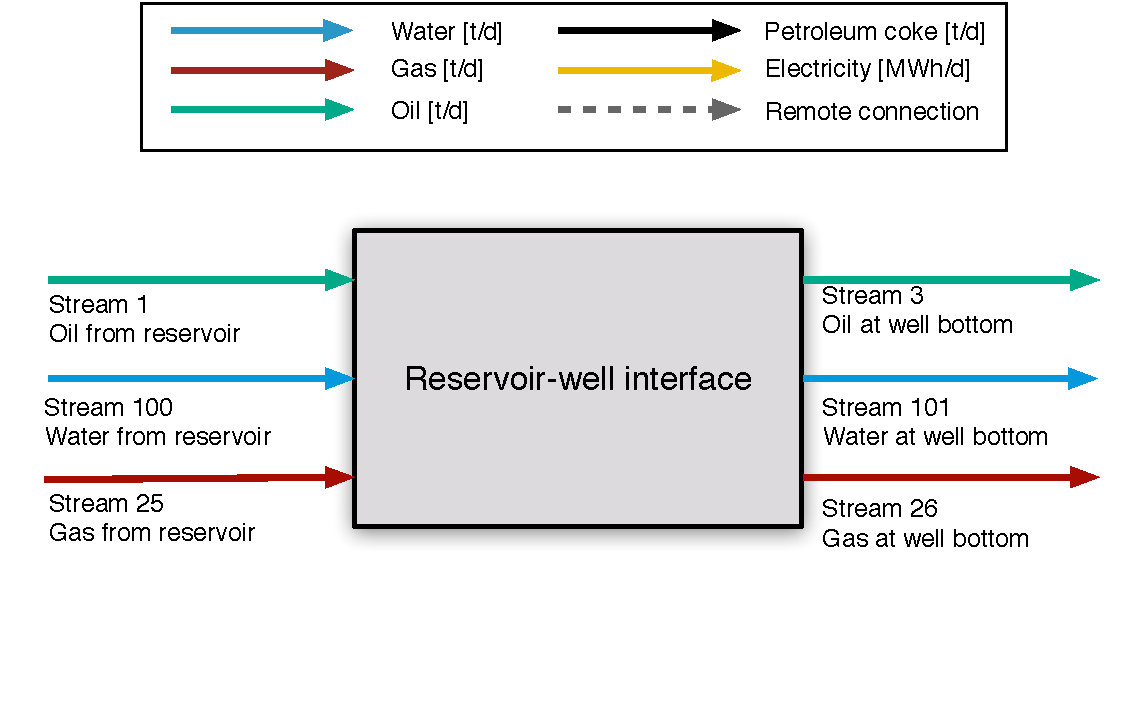
\includegraphics[width=0.85\columnwidth]{images/Reservoir_PF.pdf}
\caption{Streams flowing into and out of reservoir-well interface. All streams measured in tonnes per day excepting electricity which is measured in MWh/d.}
\label{fig:reservoir_PF}
\end{figure}
%%%%%%%%%%%

\clearpage

First, the volumetric flow rate of oil in reservoir barrels is looked up for stream \stream{1} from the flow table, \xlname{INDEX(FlowTable,Q\_O\_bbl,1)}. The method for computing crude oil density given temperature, pressure, and solution gas oil ratio is given above in the flow table description. 

The volumetric flow rate water at reservoir conditions is looked up from the flow table \xlname{INDEX(FlowTable,Q\_W\_bbl,100)} for stream \stream{100}. 

The volumetric gas flow rate at reservoir conditions is looked up from the flow table \xlname{INDEX(FlowTable,Q\_G,25)} for stream \stream{25}.

These are divided by the number of wells $N_w$ \xlname{Num\_prod\_wells} to determine flow rate in bbl for the dense phases (oil + water) and in ft$^3$ for gas. 

The expected bottomhole flowing pressure is computed in two different ways, and the lower pressure is used from these two methods. The first method uses the productivity index, \emph{PI}, defined as \cite[p. 23]{Takacs2005}:

%%%%%%%%%%
\begin{minipage}{0.6\columnwidth}\label{eq:pressure_drawdown}
\begin{fleqn}[0pt]
\begin{equation}
\emph{PI} = \frac{Q_{l,W}}{(p_{R}-p_{wf})} \quad\quad\eqnunitfrac{bbl}{psi-d}
\end{equation}
\end{fleqn}
\end{minipage}\hfill
\begin{minipage}{0.3\columnwidth}
        \begin{tabular}{|cl}
        & \\
        \emph{PI}   & \xlname{Prod\_index}\\
        $p_{R}$   & \xlname{Res\_press}\\
        & \\
        \end{tabular}
\end{minipage}
%%%%%%%%%%

where \textit{PI} = well productivity index [bbl liquid/psi-d]; $Q_{l,W}$ = liquid production per well [bbl liquid/d]; $p_{res}$ = average reservoir pressure [psi]; and $p_{wf}$ = wellbore pressure [psi]. In OPGEE a default \textit{PI} of 6.8 [bbl liquid/psi-d] is assumed to calculate the pressure drawdown. The \sheet{Active field} parameter \xlname{Prod\_index} is used to change the default \textit{PI}.

An increase in production requires an increase in pressure drawdown at a constant productivity index.  The user has to control the inputs to satisfy the condition of $p_{wf}$ $\geq$ 0.

Given the PI, the bottomhole flowing pressure is:

\begin{minipage}{0.6\columnwidth}
\begin{fleqn}[0pt]
\begin{equation} \label{eq:bottomhole_pressure}
p_{wf} =  p_{R} - \frac{Q_{o}+Q_{w}}{n_w PI}  \quad\quad\eqnunit{psi}
\end{equation}
\end{fleqn}
\end{minipage}\hfill
\begin{minipage}{0.3\columnwidth}
        \begin{tabular}{|cl}
                        & \\
        $p_{wf}$        & \xlname{Bottomhole\_flowing\_pressure}    \\    
        $p_{R}$       & \xlname{Res\_press}\\
        $Q_{o}$         & \xlname{INDEX(FlowTable,Q\_O\_bbl,1)}\\
        $Q_{w}$         & \xlname{INDEX(FlowTable,Q\_W\_bbl,100)}\\
        $n_{w}$         & \xlname{Num\_Wells}\\
        $PI$            & \xlname{Prod\_index}\\
                         & \\
        \end{tabular}
\end{minipage}

The second method estimates the pressure drop in the free gas phase. To find the bottomhole flowing pressure necessary to flow gas through the reservoir, we use the steady state radial horizontal gas flow equation in Lake \cite{Holstein2007b} (equation 10.32).

%%%%%%%%%%
\begin{equation} 
q_{g} = \frac{2 \pi k h T_{sc}}{p_{sc} T \text{ln}\left(\frac{r_2}{r_1} \right)} \int_{p_1}^{p_2} \frac{\tilde{p} \tilde{dp}}{\mu_g z} \quad\quad\eqnunitfrac{tonnes}{day}
\end{equation}
%%%%%%%%%%

Lake describes how this formula can be approximated by a set of equations according to the pressure in the reservoir. The general radial flow equation is:

%%%%%%%%%%
\begin{equation} 
q_{g} = \frac{k h}{\beta \text{ln}\left(\frac{r_2}{r_1} \right)} \Delta \psi \quad\quad\eqnunitfrac{tonnes}{day}
\end{equation}
%%%%%%%%%%

Where $\beta$ and $\Delta \psi$ are defined based on the pressure in the following table:

\begin{table}[ht]
\begin{scriptsize}
\caption{Definition of $\beta$ and $\psi$ in gas side pressure drop approximation}
\begin{tabular*}{0.8\columnwidth}{p{0.3\columnwidth}p{0.25\columnwidth}p{0.25\columnwidth}}
\toprule
Pressure range & $\beta$ & $\psi$ \\
\midrule
High (>2000 psia) & $\frac{\overline{B_g}\overline{\mu_g}}{2\pi}$ & $\Delta p$ \\
Low (<2000 psia) & $\frac{p_{sc} T \overline{\mu_g} \overline{z}}{\pi T_{sc}}$ & $\Delta p^2 = p_2^2 - p_1^2$ \\
\bottomrule
\end{tabular*}
\end{scriptsize}
\end{table}

Therefore, in OPGEE the calculation is made as follows:

At high pressure,

%%%%%%%%%%
\begin{equation} 
p_{wf} = p_e - \frac{q_g p_{sc} T z \mu_g \text{ln}\left(\frac{r_2}{r_1} \right)}{2 \pi T_{sc} p k h} \quad\quad\eqnunit{psia}
\end{equation}
%%%%%%%%%%

At low pressure,

%%%%%%%%%%
\begin{equation} 
p_{wf} = \sqrt{p_e^2 - \frac{q_g p_{sc} T z \mu_g \text{ln}\left(\frac{r_2}{r_1} \right)}{\pi T_{sc} k h}} \quad\quad\eqnunit{psia}
\end{equation}
%%%%%%%%%%
% issue 20: SPE uses w or d or e for thickness. I suggest to change h to w in eq. and in Table 7.12. I didn't change it as I am not sure if we want to re-name parameters in the main equations of text.

Here, $p_e$ is the far field pressure, $q_g$ is the gas phase fluid rate per well, $p_{sc}$ and $T_{sc}$ are pressure and temperature at standard conditions, $T$ is the reservoir temperature, $z$ is the gas z-factor, $\mu_g$ is gas viscosity, $k$ is reservoir permeability, and $h$ is pay thickness. $\left(\frac{r_2}{r_1} \right)$ is the ratio of reservoir drainage radius to wellbore radius. We set this to an arbitrarily high value (1000 ft/0.5 ft). In general, the gas phase pressure drop will be much lower than the liquid phase pressure drop, as gas flows much more readily in response to pressure differentials than liquids do.

The pressure for lifting can either be applied by a downhole pump or by gas lift; in OPGEE these methods may be used individually or simultaneously. These are described in the section below describing the \sheet{Well and downhole pump} worksheet.

\clearpage



\begin{landscape}

\begin{tiny}
\tablefirsthead{\toprule Param. & Description & Defined name & Default & Literature range & Unit & Sources & Notes\\
\midrule}
\tablehead{ \multicolumn{8}{p{1\columnwidth}}{\textit{Continued from previous page}}\\ \toprule Param. &Description & Defined name &Default & Literature range & Unit & Sources & Notes \\ 
\midrule }
\tabletail{\bottomrule \multicolumn{8}{p{1\columnwidth}}{\textit{Continued on next page...}}\\}
\tablelasttail{\bottomrule}
\tablecaption{Primary inputs used in \sheet{Reservoir} sheet.}
\label{tab:primary_inputs_reservoir}
\begin{threeparttable}
\begin{supertabular*}{1\columnwidth}{p{0.03\columnwidth}p{0.25\columnwidth}p{0.25\columnwidth}p{0.07\columnwidth}p{0.07\columnwidth}p{0.07\columnwidth}p{0.07\columnwidth}p{0.07\columnwidth}}
$PI$             & Productivity index                & \xlname{Prod\_index}  & 3         & 1-200   & [bbl/psi-d] & & \\ 
$n_w$           & Number of wells                   & \xlname{Num\_prod\_wells} & 8     & 1-10,000      & - & & \\
$p_{R}$           & Reservoir pressure                & \xlname{Res\_press}   & 1531      & 50-10,000     & [psi] & & \\
$T_{R}$ 	    & Reservoir temperature			    & \xlname{Res\_temp}  & 198.2 		& 50-300 	& [$^\circ$ F] &  & \\ 
\end{supertabular*}
%\begin{tablenotes}
%\item[a] Insert text of note here
%\end{tablenotes}
\end{threeparttable}
\end{tiny}

\newpage

\begin{tiny}
\tablefirsthead{\toprule Param. & Description & Defined name & Default & Literature range & Unit & Sources & Notes\\
\midrule}
\tablehead{ \multicolumn{8}{p{1\columnwidth}}{\textit{Continued from previous page}}\\ \toprule Param. &Description & Defined name &Default & Literature range & Unit & Sources & Notes \\ 
\midrule }
\tabletail{\bottomrule \multicolumn{8}{p{1\columnwidth}}{\textit{Continued on next page...}}\\}
\tablelasttail{\bottomrule}
\tablecaption{Secondary inputs used in \sheet{Reservoir} sheet.}
\label{tab:secondary_inputs_reservoir}
\begin{threeparttable}
\begin{supertabular*}{1\columnwidth}{p{0.03\columnwidth}p{0.25\columnwidth}p{0.25\columnwidth}p{0.07\columnwidth}p{0.07\columnwidth}p{0.07\columnwidth}p{0.07\columnwidth}p{0.07\columnwidth}}
$p_{e,i}$       & Excess pressure of injection                        & \xlname{Pressure\_excess\_injection} &   500 & 100-1,000  & [psi] &  & \\
$k_{R}$        & Permeability of reservoir                         & \xlname{Permeability\_reservoir} & 100 & 0.1 - 1000 & [mD] & & \\
$h_{R}$        & Net reservoir thickness                           & \xlname{Pay\_thickness\_reservoir}  & 50 & 10-500 & [ft] & & \\
\end{supertabular*}
%\begin{tablenotes}
%\item[a] 
%\end{tablenotes}
\end{threeparttable}
\end{tiny}

\end{landscape}




%%%%%%%%%%%%%%%%%%%%%%%%%%%%%%%%%%%%%
\section{Well and downhole pump}

Initially in the life of many fields, the pressure in the subsurface -- combined with the buoyancy of oil and gas compared to water -- is sufficient to allow fluids to flow to the surface un-aided. This phase is sometimes called ``primary production''. As production from a field proceeds the reservoir pressure will decrease. To maintain economic viability, artificial lift equipment is used to enhance production rates. Most commonly, energy is added to the reservoir fluids through the use of a downhole pump \cite[p. 2]{Takacs2005}. Another method is gas lifting, which entails injecting gas into the production string to decrease the density of the column of fluids in the production tubing. The \sheet{Well and downhole pump} sheet calculates the work required to lift the fluids to the surface.

The streams flowing into and out of the wellbore/downhole pump process are shown in Figure \ref{fig:wellbore_PF} and are listed in Table \ref{tab:reservoir_PF}.


\clearpage

%%%%%%%%%%%
\begin{table}
\caption{Streams flowing into and out of the wellbore/downhole pump process. I/O denotes input or output stream.}
\label{tab:wellbore_PF}
\begin{scriptsize}
\begin{tabularx}{1\columnwidth}{p{0.32\columnwidth}p{0.05\columnwidth}p{0.04\columnwidth}p{0.32\columnwidth}p{0.05\columnwidth}p{0.05\columnwidth}}
\toprule
Flow name							& Stream   			& I/O 	& Source/Destination       			& Units 			&  Notes\\ 
\midrule
Oil at well bottom						& \stream{3}			& I		& Reservoir/well interface			& [t/d]			&			\\
Water at well bottom						& \stream{101}			& I		& Reservoir/well interface			& [t/d]			&			\\
Gas at well bottom						& \stream{26}			& I		& Reservoir/well interface			& [t/d]			&			\\
Fuel gas - Downhole pump				& \stream{150}			& I		& Fuel gas system				& [t/d]			&			\\
Electricity - Downhole pump				& \stream{175}			& I		& Electricity generation and imports	& [MWh/d]			& 			\\
Lifting gas to wellbore					&\stream{42}			& I		& Lifting gas compressor			& [t/d]			&			\\
\midrule
Oil at wellhead							& \stream{4}			& O		& Separation					& [t/d]			&			\\
Water at wellhead						& \stream{102}			& O		& Separation					& [t/d]			&			\\
Gas at wellhead						& \stream{27}			& O		& Separation					& [t/d]			&			\\
Wellhead leaks to air						& \stream{250}			& O		& Environment - Atmosphere		& [t/d]			&			\\	
\bottomrule
\end{tabularx}
\end{scriptsize}
\end{table}
%%%%%%%%%%%


%%%%%%%%%%%
\begin{figure}
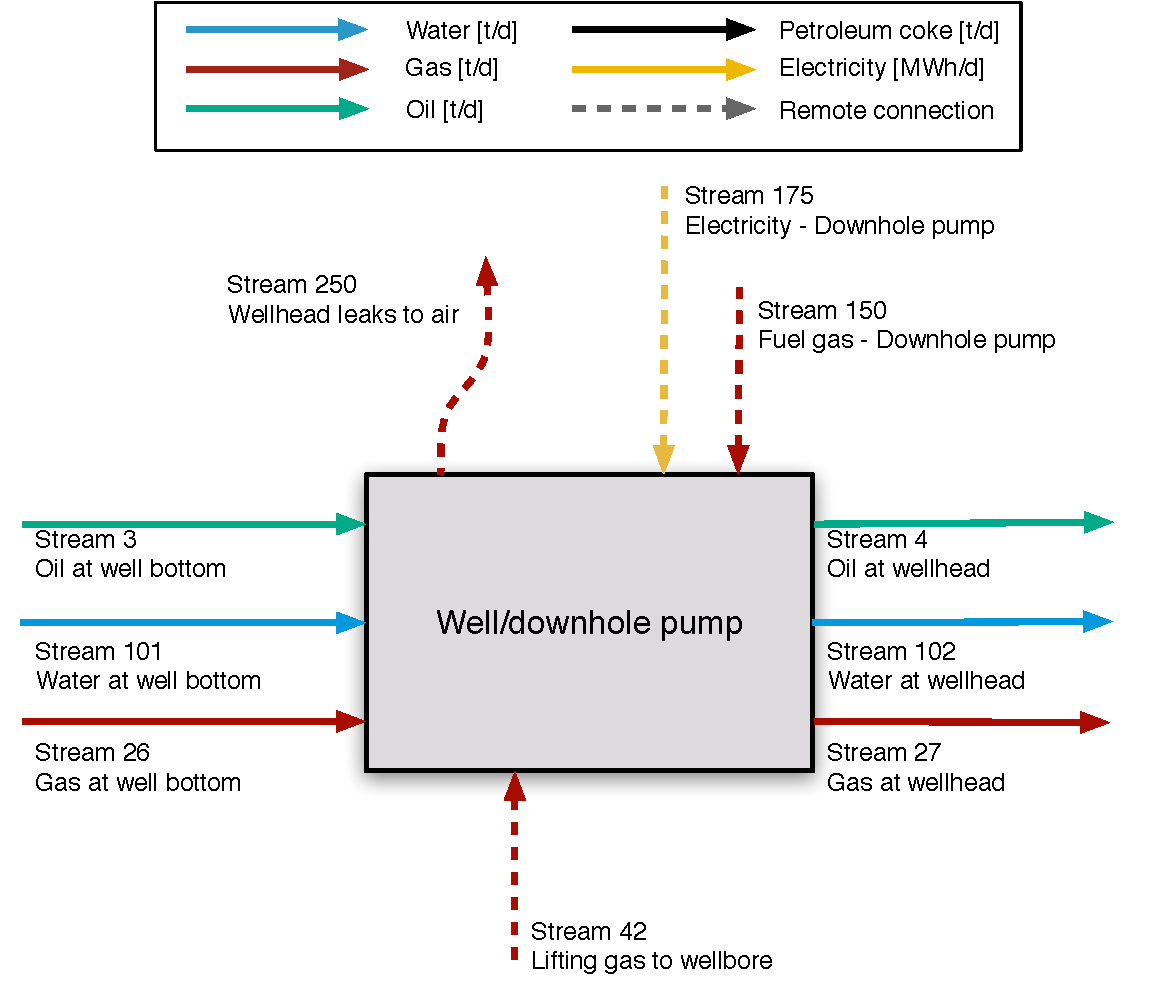
\includegraphics[width=0.85\columnwidth]{images/Wellbore_downhole_pump_PF.pdf}
\caption{Streams flowing into and out of the wellbore/downhole pump process. All streams measured in tonnes per day excepting electricity which is measured in MWh/d.}
\label{fig:wellbore_PF}
\end{figure}
%%%%%%%%%%%




\clearpage

Most common artificial lifting and improved oil recovery techniques are included in OPGEE. These include: downhole pump, gas lift, water flooding, gas flooding, and steam injection. In the \sheet{Inputs} sheet the user is prompted to choose a combination of techniques applicable to the modeled operation. 

A complete list of emissions sources from production, along with their estimated magnitude, is shown in Table \ref{tab:production_sources}.

Energy for lifting is required to overcome a pressure traverse that is in excess of the pressure available from the reservoir. The pressure traverse is the pressure drop between the subsurface reservoir and the surface wellhead. The pressure traverse arises due to two factors: (i) flow against gravity, and (ii) frictional losses. The pressure required for lifting is calculated by adding the wellhead pressure to the pressure traverse and subtracting the wellbore pressure. The artificial lifting methods that can be chosen in OPGEE are: (i) downhole pump, and (ii) gas lift. The pressure required for lifting is equal to the discharge pressure of the downhole pump. The power required to generate the required discharge pressure depends on the discharge flow rate and pump efficiency. Finally the energy required to drive the pump is calculated based on the power requirement. 

The calculation of the energy required in water injection- and gas injection- based EOR uses the user inputs for injection volume and discharge pressure. Smart defaults are in place to help assign the discharge pressure taking into account the well depth and frictional losses. 

The energy required for steam flooding requires rigorous modeling of steam generation. An additional complexity is caused by the modeling of electricity co-generation at steam projects. These calculations are explained in Section\,\ref{sec:steamgeneration}, which covers steam generation emissions.

In the case of gas lift, if the user enters the volume of gas injected and the discharge pressure, OPGEE will compute the compression energy. However, OPGEE is not sensitive to changes in the gas lift, i.e. the dynamics between the volume of gas lift and the lifting head are not considered. The calculation of these dynamics is beyond the scope of a linear GHG estimator. This requires a two phase flow model, which is not included in OPGEE \version. Thus, outside calculations are required to estimate the volume of gas lift gas required to be injected, which can then be inserted into OPGEE.

% list of the parameters used is shown in Table\,\ref{tab:production_calculations_parameters}. 

First, average properties of the fluids along the wellbore are computed. The average pressure along the wellbore is computed as:

\begin{minipage}{0.6\columnwidth}
\begin{fleqn}[0pt]
\begin{equation} \label{eq:avg_wellbore_pressure}
p_{w,avg} =  \frac{p_{wf}+p_{wh}}{2}  \quad\quad\eqnunit{psi}
\end{equation}
\end{fleqn}
\end{minipage}\hfill
\begin{minipage}{0.3\columnwidth}
        \begin{tabular}{|cl}
                        & \\
        $p_{wf}$       & \xlname{Bottomhole\_flowing\_pressure}\\
        $p_{wh}$        & \xlname{Wellhead\_pressure}\\
                         & \\
        \end{tabular}
\end{minipage}

Other averaged properties are computed by averaging items looked up from the Flow table. For example, for average solution gas-oil-ratio $R_{os,avg}$ is given by:

\begin{minipage}{0.6\columnwidth}
\begin{fleqn}[0pt]
\begin{equation} \label{eq:avg_solution_GOR}
R_{os,avg} =  \frac{R_{os,wf}+R_{os,wh}}{2}  \quad\quad\eqnunit{psi}
\end{equation}
\end{fleqn}
\end{minipage}\hfill
\begin{minipage}{0.3\columnwidth}
        \begin{tabular}{|cl}
                        & \\
        $R_{wf}$       & \xlname{INDEX(FlowTable,GOR\_OS,3)}\\
        $R_{wh}$        & \xlname{INDEX(FlowTable,GOR\_OS,4)}\\
                         & \\
        \end{tabular}
\end{minipage}
where the condition at stream \stream{3} represents the bottomhole crude oil conditions and at stream \stream{4} represents the wellhead crude oil conditions.

Other averaged properties include: 
\begin{itemize}
    \item Temperature (all phases) $T_R$ (\xlname{Wellhead\_temperature},\xlname{Res\_temp})
    \item Density of crude oil $\rho_o$ (\xlname{INDEX(FlowTable,RHO\_O\_LB,3)},\xlname{INDEX(FlowTable,RHO\_O\_LB,4)})
    \item Volume of crude oil lifted $V_o$ (\xlname{INDEX(FlowTable, Q\_O\_bbl,3)},\xlname{INDEX(FlowTable,Q\_O\_bbl,4)}) 
    \item Density of water $\rho_w$ (\xlname{INDEX(FlowTable,RHO\_W\_LB,3)},\xlname{INDEX(FlowTable,RHO\_W\_LB,4)})
    \item Volume of water lifted $V_w$ (\xlname{INDEX(FlowTable, Q\_W\_bbl,3)},\xlname{INDEX(FlowTable,Q\_W\_bbl,4)}) 
\end{itemize}

Additionally, the volume of free gas -- gas not in solution with oil -- $V_g$ is computed using similar methods to those used in the flow sheet (see above).

The area of the the production tubing cross section is computed from the production tubing radius (\xlname{Well\_diam}/2) and the total production tubing volume is computed as follows:

\begin{minipage}{0.6\columnwidth}
\begin{fleqn}[0pt]
\begin{equation} \label{eq:tubing_volume}
V_{W} =  \pi \left(\frac{D_{W}}{2}\right)^2 D_w  \quad\quad\eqnunit{psi}
\end{equation}
\end{fleqn}
\end{minipage}\hfill
\begin{minipage}{0.3\columnwidth}
        \begin{tabular}{|cl}
                        & \\
        $d_{W}$         & \xlname{Well\_diam}\\
        $D_W$           & \xlname{Field\_depth}\\
                        & \\
        \end{tabular}
\end{minipage}

Given the total volume of fluids lifted $V_{tot} = V_{o} + V_{w}+ V_{g}$ (oil, water , gas [ft$^3$/day] at average of well depth) the velocity of the fluids is computed as the total volume lifted per day divided by the cross sectional area. 

The volume-weighted density of fluids in the wellbore is computed as:

\begin{minipage}{0.6\columnwidth}
\begin{fleqn}[0pt]
\begin{equation} \label{eq:avg_wellbore_density}
\rho_{avg} =  \rho_o \frac{V_{o}}{V_{tot}}+ \rho_w \frac{V_{w}}{V_{tot}} + \rho_g \frac{V_{g}}{V_{tot}} \quad\quad\eqnunit{psi}
\end{equation}
\end{fleqn}
\end{minipage}\hfill
\begin{minipage}{0.3\columnwidth}
        \begin{tabular}{|cl}
                        & \\
                        $V_o$ & (\xlname{INDEX(FlowTable, Q\_O\_bbl,3 and 4)}) \\
                      $V_w$ & (\xlname{INDEX(FlowTable, Q\_W\_bbl,3 and 4)}) \\
                      $V_G$ & (\xlname{INDEX(FlowTable, Q\_G\_bbl,3 and 4)}) \\
                       & \\
        \end{tabular}
\end{minipage}

The weight of the fluids in the wellbore is then computed using the average fluid density in the wellbore $\rho_{avg}$ and the wellbore volume $V_W$.

\subsubsection{Well pressure traverse}

The pressure traverse is the total pressure required to lift the crude oil mixture against gravity and overcome friction and kinetic losses. This is equal to the pressure drop along the well tubing from the wellbore to the wellhead. This pressure drop has two main components: (i) the elevation component, which is the pressure drop due to gravity; and (ii) the friction component, which is the pressure drop due to liquid contact with the inner walls of the well tubing.

The total pressure traverse is equal to the total head as per: 
%%%%%%%%%%
\begin{equation} \label{eq:total_head}
p_{trav,tot}= p_{el} + p_{f} \quad\quad\eqnunit{psi}
\end{equation}
%%%%%%%%%%
where $p_{trav,tot}$ = total pressure traverse [\unit{psi}]; $p_{el}$ = pressure due to elevation change (graviational head) [\unit{ft}]; and $p_{f}$ = friction pressure drop [\unit{ft}]. 

The gravitational head pressure is \cite[Table 1, p. 455]{Mcallister2009}:
%%%%%%%%%%
\begin{equation} \label{eq:pressure_traverse}
p_{el} = \frac{\rho_{avg} V_{W}}{A_W}  \quad\quad\eqnunit{psi}
\end{equation}
%%%%%%%%%%
where $\rho_{avg}$ is the average fluid density along the wellbore column [\unitfrac{lb}{ft$^3$}], $V_{W}$ is the volume of the wellbore production tubing [\unit{ft$^3$}], and $A_W$ is the cross sectional area of the wellbore production tubing [\unit{ft$^2$}].

The frictional pressure drop is calculated using the Darcy formula \cite[p. 447]{Mcallister2009}:
%%%%%%%%%%
\begin{equation} \label{eq:friction_head}
p_{f}=\frac{fh_{el}{v_{l,W}^2}}{2d_{W}{g_{c}}} \quad\quad\eqnunit{psi}
\end{equation}
%%%%%%%%%%
where $f$ = Moody friction factor [-]; $h_{el}$ = well depth [\unit{ft}]; $v_{l,W}$ = pipeline flow velocity [\unitfrac{ft}{s}]; $D_{P}$ = pipeline diameter [\unit{ft}]; and $g_{c}$ = gravitational constant, 32.2 [\unitfrac{lbm-ft}{lbf-$s^2$}]. A major determinant of friction losses is the pipeline diameter or production tubing diameter ($d_{w}$). API production tubing diameters range from 1.05 to 4.5 inches ID; the API system is a petroleum industry standardized measuring system \cite[p. 106]{Clegg2007}.

A Moody friction factor chart is shown in Figure\,\ref{fig:Moody_chart} \cite{Moody2008}. $f$ varies with the Reynold's Number (Re) and/or pipeline roughness, depending on whether the flow regime is laminar or turbulent \cite[p. 481]{Mcallister2009}. Table\,\ref{tab:NRe_ranges} shows the Re ranges of different flow patterns. 

The Moody friction factor is estimated using simplifications for the default case as follows: Water and oil are assigned viscosities of 1 and 10 cP, respectively. The viscosity of the oil-water mixture is assigned the volume-weighted viscosity of the two fluids.\footnote{This simplification does not account for the complexity of oil-water mixture viscosity, but is used as a first-order approximation. Heavy oil can have very high viscosities as well.} 

The Reynolds number, Re, is calculated as follows \cite[p. 46]{Guo2007}:
\begin{equation}\label{eq:Nre}
\textrm{Re} = \frac{1.48 Q_l \rho_l}{d_P \mu_l} \quad\quad\eqnunit{-}
\end{equation} 

where $Q_l$ is the total liquid production rate [bbl/d]; $\rho_l$ is the liquid density (oil-water mixture) [lbm/ft$^3$]; $d_P$ is the wellbore production diameter [in], and $\mu_l$ is the fluid viscosity [cP]. Roughness of commercial steel of 0.0018 in is assumed \cite{Cengel2005}, for a relative roughness $r$ of 0.0006. The approximate friction factor is calculated as follows \cite[p. 625]{Cengel2005}:
\begin{equation}\label{eq:fric_factor}
f = \left( \frac{-1}{1.8\log\left(\left[ \frac{6.9}{\textrm{Re}}\right] + \left[ \frac{r}{3.7} \right]^{1.11} \right) } \right)^{2} \quad\quad\eqnunit{-}
\end{equation} 

This equation gives a friction factor $f$ of 0.02 for default conditions. The friction factor (\xlname{Friction\_factor}) is a user input on the \sheet{Secondary Inputs} worksheet and can be adjusted by the user. 

\begin{figure}
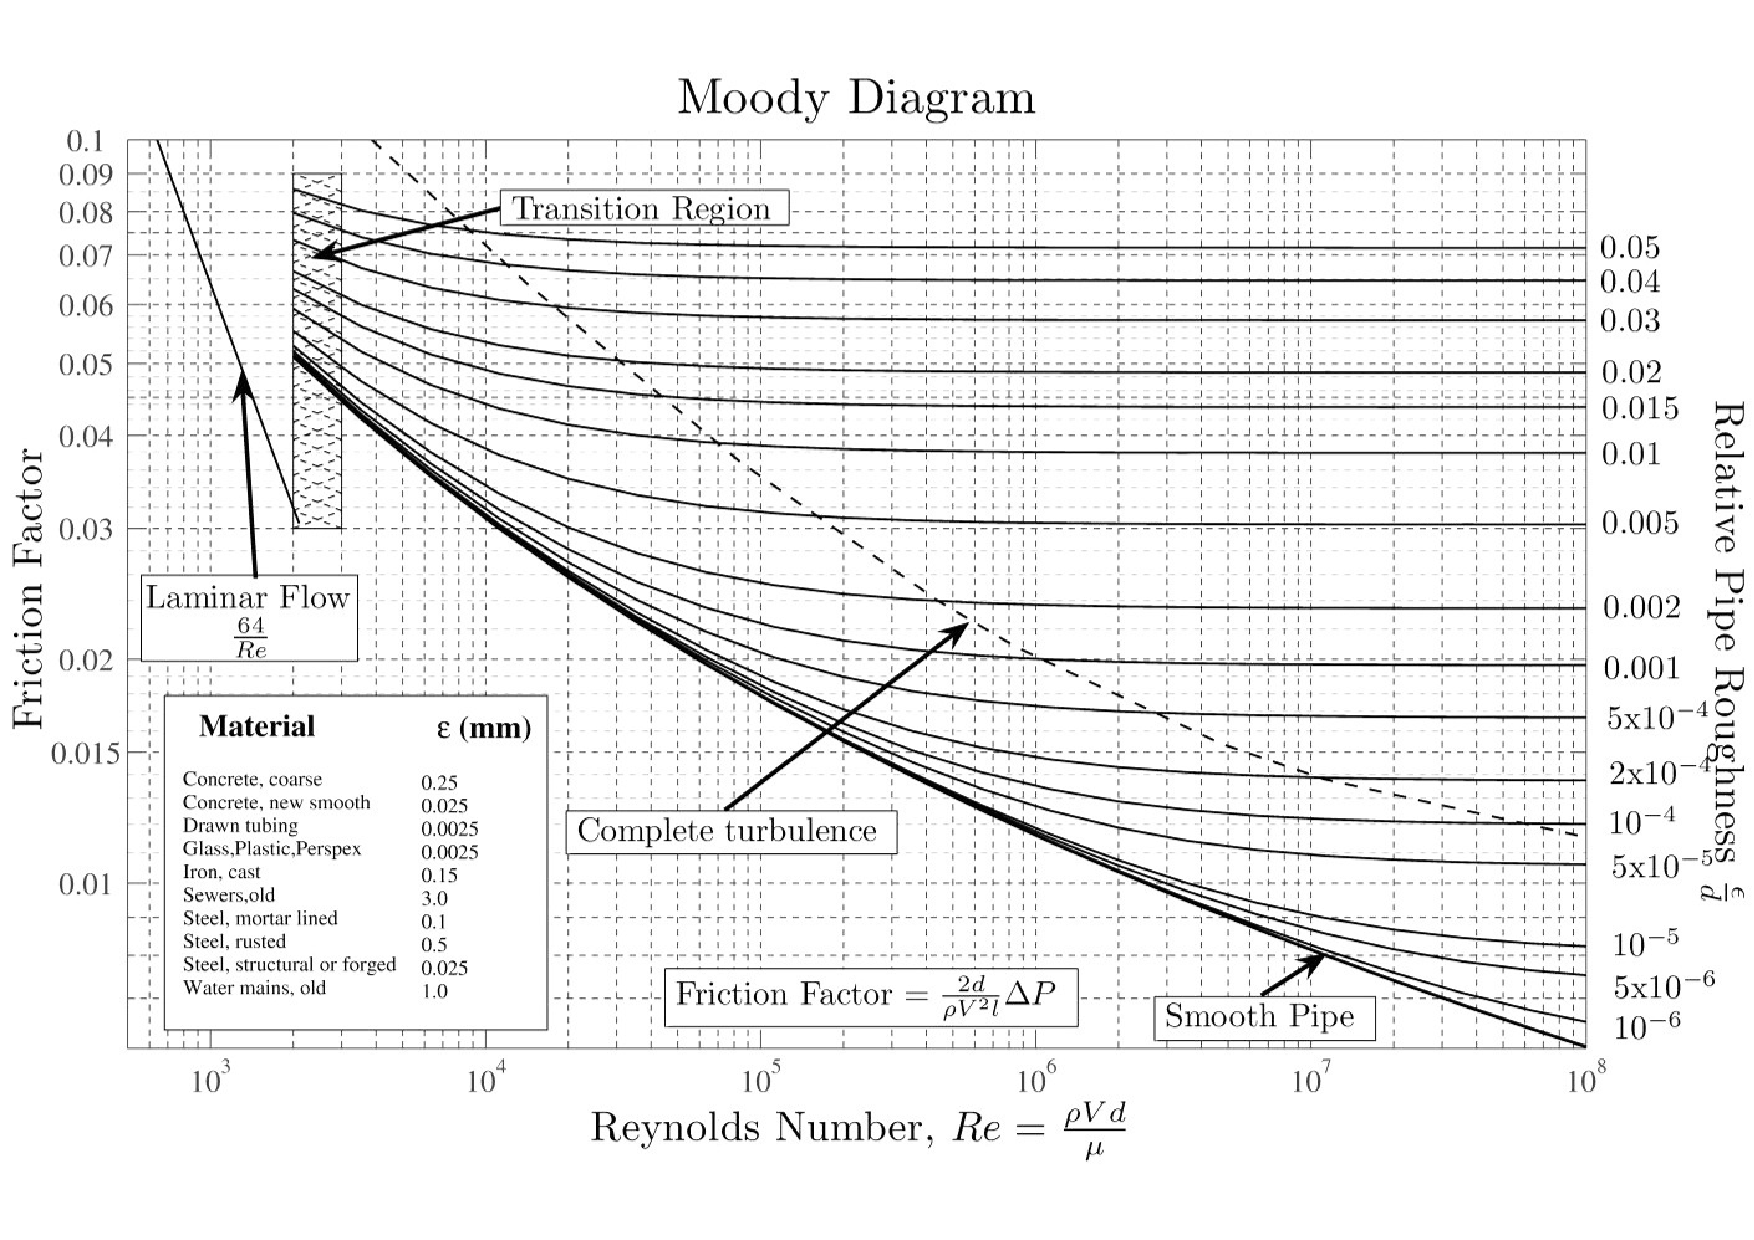
\includegraphics[width=0.95\columnwidth]{images/Moody_chart.pdf}
\caption{Moody friction factor chart. Source: \cite{Moody2008}.}
\label{fig:Moody_chart}
\end{figure}

\begin{table}
\begin{scriptsize}
\caption{Reynold's number (Re) ranges of different flow patterns. Data from McAllister \cite{Mcallister2009}.}
\label{tab:NRe_ranges}
\begin{tabular*}{0.75\columnwidth}{p{0.4\columnwidth}p{0.35\columnwidth}}
\toprule
Flow pattern & Re [-] \\
\midrule
Laminar flow & Re$<$2000 \\
Transition flow & 2000$\leq$Re$\leq$4000 \\
Turbulent flow & Re$>$ 4000 \\
\bottomrule
\end{tabular*}
\end{scriptsize}
\end{table}



\subsubsection{Pressure for lifting}

The second step after estimating pressure traverse is the calculation of the pressure for lifting which is the pressure required by artificial means (e.g., pump) to lift the oil-water mixture to the surface at the desired wellhead pressure. The pressure for lifting is calculated as:
%%%%%%%%%%
\begin{equation} \label{eq:pressure_lifting}
p_{lift}=(p_{trav,tot}+p_{wh})-p_{wf} \quad\quad\eqnunit{psi}
\end{equation}
%%%%%%%%%%
where $p_{lift}$ = pressure for lifting [\unit{psi}]; $p_{tav,tot}$ = total pressure traverse [\unit{psi}]; $p_{wh}$ = wellhead pressure [\unit{psi}] (\xlname{Wellhead\_pressure}); and $p_{wf}$ = bottomhole pressure [\unit{psi}]. The wellbore pressure is calculated from the average reservoir pressure by subtracting the pressure drawdown. The pressure drawdown is the difference between the reservoir pressure and the bottomhole pressure \cite[p. 22]{Takacs2005}.

\subsubsection{Pump brake horsepower} \label{sec:brake horsepower}

The brake horsepower (BHP) is calculated using the pump discharge flow rate and the pumping pressure as \cite[p. 27]{Rose1989}: 
%%%%%%%%%%
\begin{equation} \label{eq:pump_BHP}
\begin{split}
&\text{BHP$_{P}$}=\frac{1.701 \times 10^{-5} Q_{d} \Delta p}{\eta_P} \begin{footnotesize} \quad\quad\eqnunit{hp} \end{footnotesize}\\
&\text{This is equivalently expressed as:}\\
&\text{BHP$_{P}$ [hp]}=\frac{\frac{1 [\text{hp}]}{1714 [\text{gpm-psi}]} \frac{42\left[\frac{\text{gal}}{\text{bbl}}\right]}{24\left[\frac{\text{hr}}{\text{d}}\right] 60\left[\frac{\text{min}}{\text{hr}}\right]} Q_{d} \left[\frac{\text{bbl}}{\text{d}}\right] \Delta p [\text{psi}]}{\eta_P} 
\end{split}
\end{equation}
%%%%%%%%%%
where BHP$_{P}$ = brake horsepower [hp]; $Q_{d}$ = pump discharge rate [bbl/d]; \newline $\Delta p$ = pumping pressure [psi]; and $\eta_P$ = pump efficiency [\%] (\xlname{Eta\_pump\_well}. The term 1714 is a dimensionless factor that converts between [hp] and [gpm-psi]. The pumping pressure is the difference between pump discharge and suction pressures. The default suction pressure is 0 psi. In the case of a downhole pump the pumping pressure is equal to the pressure for lifting as calculated in eq.\ \eqref{eq:pressure_lifting}. 

\subsection{Defaults for well and downhole pump}

Default values for reservoir calculations are shown in Tables \ref{tab:primary_inputs_downholepump}, and \ref{tab:secondary_inputs_downholepump}. 

\begin{landscape}

\begin{tiny}
\tablefirsthead{\toprule Param. & Description & Defined name & Default & Literature range & Unit & Sources & Notes\\
\midrule}
\tablehead{ \multicolumn{8}{p{1\columnwidth}}{\textit{Continued from previous page}}\\ \toprule Param. &Description & Defined name &Default & Literature range & Unit & Sources & Notes \\ 
\midrule }
\tabletail{\bottomrule \multicolumn{8}{p{1\columnwidth}}{\textit{Continued on next page...}}\\}
\tablelasttail{\bottomrule}
\tablecaption{Primary inputs used in \sheet{Well and downhole pump} sheet.}
\label{tab:primary_inputs_downholepump}
\begin{threeparttable}
\begin{supertabular*}{1\columnwidth}{p{0.03\columnwidth}p{0.25\columnwidth}p{0.25\columnwidth}p{0.07\columnwidth}p{0.07\columnwidth}p{0.07\columnwidth}p{0.07\columnwidth}p{0.07\columnwidth}}
$d_{w}$ 	    & Well production tubing diameter	& \xlname{Well\_diam}  & 2.775 		& 1 - 4.5	& [in] &  & \\ 
$D_{w}$         & Field depth                       & \xlname{Field\_depth} & 7,122      & 100-20,0000   & [ft] & & \\ 
$n_w$           & Number of wells                   & \xlname{Num\_prod\_wells} & 8     & 1-10,000      & - & & \\
$Q_o$           & Production rate of oil            & \xlname{Oil\_prod}    & 1,500     & 10-3,000,000  & [bbl/d] & & \\
$GOR$          & Gas oil ratio, producing          & \xlname{GOR}          & var.      & 5-100,000     & [scf/bbl] & & \\
$T_{R}$ 	    & Reservoir temperature			    & \xlname{Res\_temp}  & 198.2 		& 50-300 	& [$^\circ$ F] &  & \\ 
\end{supertabular*}
%\begin{tablenotes}
%\item[a] Insert text of note here
%\end{tablenotes}
\end{threeparttable}
\end{tiny}

\newpage

\begin{tiny}
\tablefirsthead{\toprule Param. & Description & Defined name & Default & Literature range & Unit & Sources & Notes\\
\midrule}
\tablehead{ \multicolumn{8}{p{1\columnwidth}}{\textit{Continued from previous page}}\\ \toprule Param. &Description & Defined name &Default & Literature range & Unit & Sources & Notes \\ 
\midrule }
\tabletail{\bottomrule \multicolumn{8}{p{1\columnwidth}}{\textit{Continued on next page...}}\\}
\tablelasttail{\bottomrule}
\tablecaption{Secondary inputs used in \sheet{Well and downhole pump} sheet.}
\label{tab:secondary_inputs_downholepump}
\begin{threeparttable}
\begin{supertabular*}{1\columnwidth}{p{0.03\columnwidth}p{0.25\columnwidth}p{0.25\columnwidth}p{0.07\columnwidth}p{0.07\columnwidth}p{0.07\columnwidth}p{0.07\columnwidth}p{0.07\columnwidth}}
$C_{w,TDS}$    & Concentration of total dissolved solids in water       & \xlname{W\_TDS} &   5,000 & 0-50,000  & [mg/L] & \cite{Vlasopoulos2006} & \\
$f$             & Moody friction factor                                 & \xlname{Friction\_factor} & 0.02 & 0.01 - 0.1 & - & & \\
$O_{pm,w}$       & Option for prime mover type, well                    & \xlname{Prime\_mover\_type\_well}  & 1 & 1-4 & - & & \\
$p_{wh}$        & Wellhead pressure                                     & \xlname{Wellhead\_pressure} & 1,000 & 50-2,000  & [psi] & & \\
$T_{wh}$        & Wellhead temperature                                  & \xlname{Wellhead\_temperature} & 150 & 50-200 & [$^\circ$] & & \\
$\eta_{pump}$   & Efficiency of downhole pump                           & \xlname{Eta\_pump\_well}  & 65    & 50-80 & [\%] & & \\
\end{supertabular*}
%\begin{tablenotes}
%\item[a] 
%\end{tablenotes}
\end{threeparttable}
\end{tiny}

\end{landscape}



\clearpage

%%%%%%%%%%%%%%%%%%%%%%%%%%%%%%
\section{Bitumen mining}
\label{sec:bitumen_mining}

Bitumen mining takes in raw bitumen ore (containing sand, bitumen, and water) and produces cleaned and separated bitumen ready for upgrading or dilution.

The streams flowing into and out of the bitumen mining process are shown in Figure \ref{fig:mining_PF} and are listed in Table \ref{tab:mining_PF}.


\clearpage

%%%%%%%%%%%
\begin{table}
\caption{Streams flowing into and out of the bitumen mining process. I/O denotes input or output stream.}
\label{tab:mining_PF}
\begin{scriptsize}
\begin{tabularx}{1\columnwidth}{p{0.32\columnwidth}p{0.05\columnwidth}p{0.04\columnwidth}p{0.32\columnwidth}p{0.05\columnwidth}p{0.05\columnwidth}}
\toprule
Flow name							& Stream   			& I/O 	& Source/Destination       			& Units 			&  Notes\\ 
\midrule
Bitumen at mine						& \stream{2}			& I		& Bitumen mine				& [t/d]			&			\\
Fuel gas - Mining						& \stream{167}			& I		& Fuel gas system				& [t/d]			&			\\
Electricity - Mining						& \stream{193}			& I		& Electricity generation and imports	& [MWh/d]			& 			\\
\midrule
Bitumen from mine to upgrader				& \stream{5}			& O		& Separation					& [t/d]			&			\\
Bitumen from mine to dilution				& \stream{6}			& O		& Separation					& [t/d]			&			\\
Mine offgas to flare						& \stream{84}			& O		& Environment - Atmosphere		& [t/d]			&			\\
Mine face fugitives and tailings pond emissions			& \stream{281}			& O	& Environment - Atmosphere		& [t/d]			&			\\	
\bottomrule
\end{tabularx}
\end{scriptsize}
\end{table}
%%%%%%%%%%%


%%%%%%%%%%%
\begin{figure}
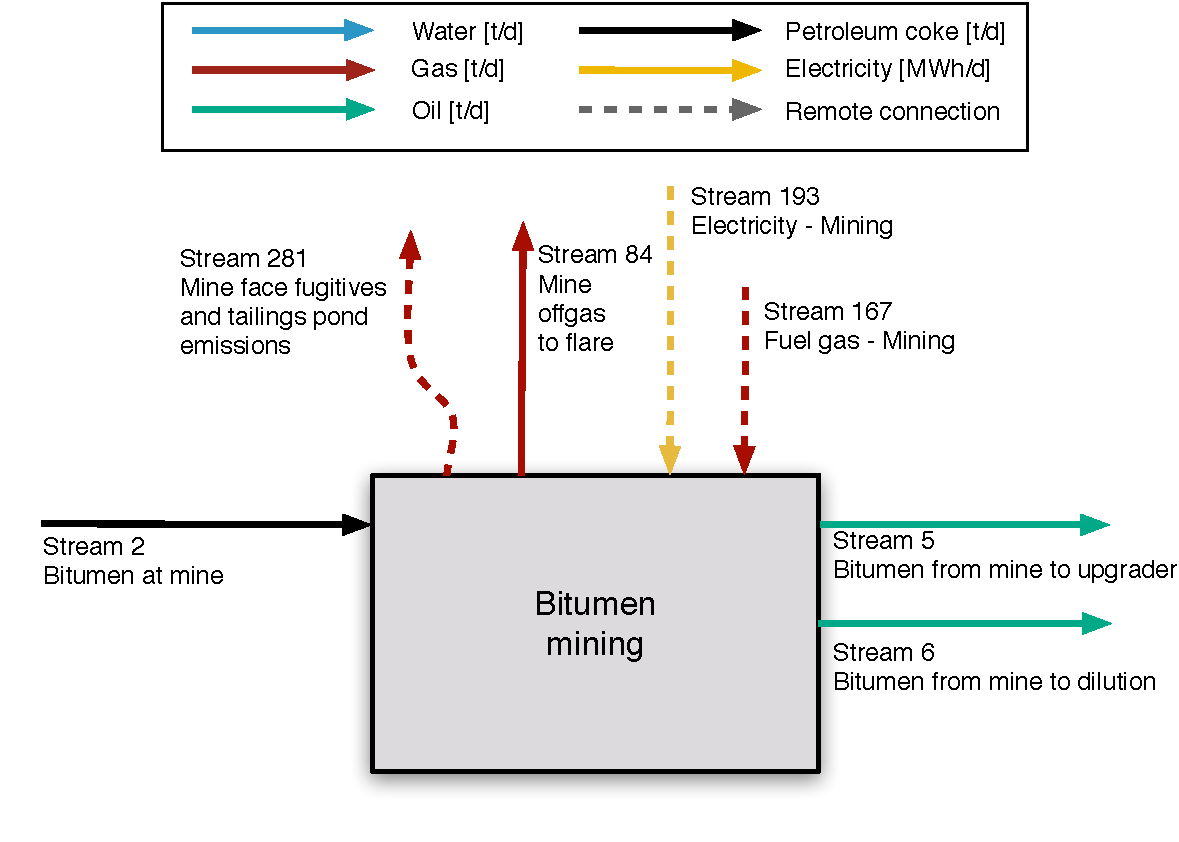
\includegraphics[width=0.85\columnwidth]{images/Bitumen_Mining_PF.pdf}
\caption{Streams flowing into and out of the bitumen mining process. All streams measured in tonnes per day excepting electricity which is measured in MWh/d.}
\label{fig:mining_PF}
\end{figure}
%%%%%%%%%%%

\clearpage


The characteristics of major bitumen mining operation are summarized in Table \ref{tab:bitumen_mining_data}. One of the main differences between oil sands mines is the bitumen froth treatment technology used. Once oil sands material is mined it is transported to a separation facility where hot water is added to produce an oil sands slurry. The slurry is brought to an extraction facility where gravity drainage is used to remove larger solids and produce a bitumen froth, a mixture of bitumen, fine solids, and water. This bitumen froth undergoes froth treatment, in which a light hydrocarbon (either naphthenes or paraffins) acts as a solvent and separates bitumen from other material contained in the bitumen froth.  Older projects (those constructed prior to 2002) all employ naphthenic froth treatment (NFT), while projects constructed from 2002 onwards (with the exception of the CNRL Horizon project which employs NFT) employ paraffinic froth treatment (PFT).  

The bitumen produced at NFT facilities is of lower quality, containing a higher percentage of asphaltenes and more residual water and solids. Bitumen produced at NFT mines must therefore go through upgrading to synthetic crude oil (SCO) and cannot be diluted and sent directly to refineries, as is the case for bitumen produced at PFT facilities. Generally NFT mines include an upgrader located at the mine site. Because natural gas and electricity consumed for the mine and the upgrader are delivered to the site altogether, the facilities share a common cogeneration system and a significant amount of waste heat from the upgrader is used in the bitumen separation process. 

Disentangling use by mining operations alone is challenging given the complex nature of operations. Importantly, the Alberta Energy Regulator (AER) reports natural gas and electricity consumption for integrated mining and upgrading facilities together without specifying the quantities of natural gas and electricity consumed for mining alone. The exception to this is the Syncrude Aurora (NFT) project, as bitumen produced at that site is transported to the Syncrude Mildred Lake (NFT) project for upgrading at the Mildred Lake upgrading facility.  Also, the Suncor upgrader located at the mine site also upgrades bitumen produced at Suncor's Firebag in situ project.  Bitumen produced by the stand-alone Shell Muskeg River and Jackpine (PFT) mines is upgraded at the stand-alone Shell Scotford upgrader, however as the upgrader is located off-site the energy consumption for the mines is reported separately from the upgrading process. The Imperial Kearl project is the only mining project that produces diluted bitumen (known as dilbit) that is sent directly to refineries without undergoing any intermediate upgrading.  Of all the mining projects, the Suncor upgrader produces some diesel fuel that is combusted as a fuel on-site.

\begin{table}
\caption{Characteristics of operating mining projects.}
\label{tab:bitumen_mining_data}
\begin{scriptsize}
\begin{tabularx}{1\columnwidth}{p{0.2\columnwidth}p{0.05\columnwidth}p{0.05\columnwidth}p{0.05\columnwidth}p{0.05\columnwidth}p{0.4\columnwidth}}
\toprule
Mine						& Year & Cap. (bbl/d) & Sep. & Int. upgr.? & Notes \\
\midrule
Suncor					& 1967	& 490,000		& NFT	& Yes	&Upgrader also processes bitumen produced from Suncor Firebag in situ project. \\
Syncrude Mildred Lake		& 1978	& 150,000		& NFT	&Yes		& Upgrader also processes bitumen produced at Syncrude Aurora mine. \\
Syncrude Aurora			& 2001	& 200,000		& NFT	& No		& Waste heat from Syncrude Mildred Lake upgrader used in Syncrude Aurora mine. \\
CNRL Horizon				& 2008	& 250,000		& NFT	& Yes	& \\				
Shell Muskeg River			&2002	& 155,000		& PFT	& No		& Bitumen transported to stand-alone Shell Scotford upgrader. \\
Shell Jackpine				& 2010	& 100,000		& PFT	& No		& Bitumen transported to stand-alone Shell Scotford upgrader. \\
Imperial Kearl				& 2013	& 220,000		& PFT	& No		& Only mine that produces diluted bitumen. \\
\bottomrule
\end{tabularx}
\end{scriptsize}
\end{table}

\paragraph{Public Data Available}

Data are available from a number of public sources.  First, the AER publishes monthly Statistical Reports on oil sands operations. Most useful are ST39: \emph{Alberta Mineable Oil Sands Plant Statistics}, which was published from 1970-2002 and 2008-2014 \cite{AERvar}; as well as ST43: \emph{Alberta Oil Mineable Oil Sands Plant Statistics - Annual}, which was published in years 2003-2007 \cite{AERvarSt43}. These statistical reports tabulate monthly energy consumption, flared/wasted fuels, and electricity, bitumen, and SCO production for each oil sands project. Some projects operated by the same company receive fuel at one mine and then deliver fuel to the other mine and so report the total fuel consumption under the mine that receives the fuel (e.g., Syncrude's Mildred Lake and Aurora projects) rather than reporting the fuel consumption for each project separately \cite{AER2016}.
 
Definitions provided by AER for energy consumption reported in the AER's ST39 and ST43 reports include definitions of some potentially ambiguous data \cite{AER2016}:
\begin{itemize}
\item SCO Fuel Use: The total volume of SCO combusted as fuel at the facility.
\item SCO Plant Use: The total volume of SCO used at the facility for uses other than fuel.
\item Bitumen Flared/Wasted: The total volume of unrecovered crude bitumen from spills, upgrading slops, tanks dewatering etc.
\end{itemize}
Note that diesel fuel consumption for each project is collected by the AER but not reported in any of the AER's reports \cite{AER2016}. One project, Suncor, does report that the upgrader produces diesel fuel that is used as fuel on site for mining operations. This use is reported under the AER as SCO fuel consumption \cite{AERvar}.

Another important data source are engineering ``templates'' generated by the Canada's Oil Sands Innovation Alliance (COSIA). COSIA has published two mine templates that contain material and energy flow diagrams for the two froth treatment technologies (naphthenic froth treatment and paraffinic froth treatment) employed in the oil sands \cite{COSIA2015a, COSIA2015b}. For each froth treatment technology, energy and material flows are presented for two possible oil sands ore qualities: low grade ore at 9 wt.\% bitumen, and high grade ore at 12 wt.\%. The COSIA Mine Templates provide approximate energy consumption values for a representative mining project based on existing oil sands operations but not representative of any currently operating oil sands project.

A last source of data is the Alberta Environmental Monitoring, Evaluation, and Reporting Agency (AEMERA), which has published estimates of fugitive GHG emissions from mine face, tailings ponds, and `other' (e.g., emissions from pipe fitting and equipment leaks, releases from pressure relief valves, tanks, and sewage lagoons) for each oil sands company operating a mining project from January 1st, 2011 to December 31st, 2014 \cite{AEMERA2015}. The fugitive GHG emissions generated by AEMERA are developed from figures reported by companies to the Government of Alberta under the Specified Gas Emitters Regulation (AB, 2007). The estimated fugitive CH$_4$ emissions from oil sands mine face and tailings ponds reported by AEMERA are close to the numbers reported elsewhere \cite{Johnson2016, GHGenius4.03}.

In order to capture the range of mining projects, OPGEE models two template mining operations: 
\begin{itemize}
\item an upgrader-integrated mine using naphthenic froth treatment (NFT) separation technology;
\item A stand-alone mine using paraffinic froth treatment (PFT) separation technology.
\end{itemize}

As can be seen in Table \ref{tab:bitumen_mining_data} above, the integrated mine and upgrader using NPT separation is more indicative of older large-scale mining projects developed in the 1970s and 1980s, such as the Suncor and Syncrude operations.  Additionally, the more recently developed CNRL Horizon project is an integrated NFT mine.  The non-integrated mine with PFT separation is more representative of modern developments such as Albian Sands (Shell), Aurora (Syncrude), Jackpine (Shell), and Kearl (Imperial). 

Public natural gas and electricity consumption literature data available, AER facility-reported data and COSIA Mine Template ranges, is presented in Figures \ref{fig:mining_ng} and \ref{fig:mining_elec}, respectively, below. Production-weighted average energy consumption is reported for both 2014 and over the project life based on the AER data reported for each facility. The shaded regions represent the natural gas consumption for NFT and PFT mines presented in the COSIA Mine Template for low grade and high grade ore. Note that no corresponding graph can be created for diesel consumption due to lack of consistent reporting of diesel use in AER datasets.

There is some challenge in interpreting reported public data. First, note that natural gas consumption reported by AER for Suncor, Syncrude Mildred Lake, and CNRL Horizon mines includes natural gas consumed in on-site upgraders. Similarly, electricity consumption reported by AER for Suncor, Syncrude Mildred Lake, and CNRL Horizon mines include electricity consumed in on-site upgraders. Lastly, the Shell Muskeg River mine receives the majority of natural gas that is consumed at Shell Jackpine mine, meaning that per-mine consumption at each Shell mine is between the two reported values (high for Muskeg River and very low for Jackpine).  The separation of stand-alone vs.\ integrated upgrading mines, is discussed more fully below.


\begin{figure}[t]
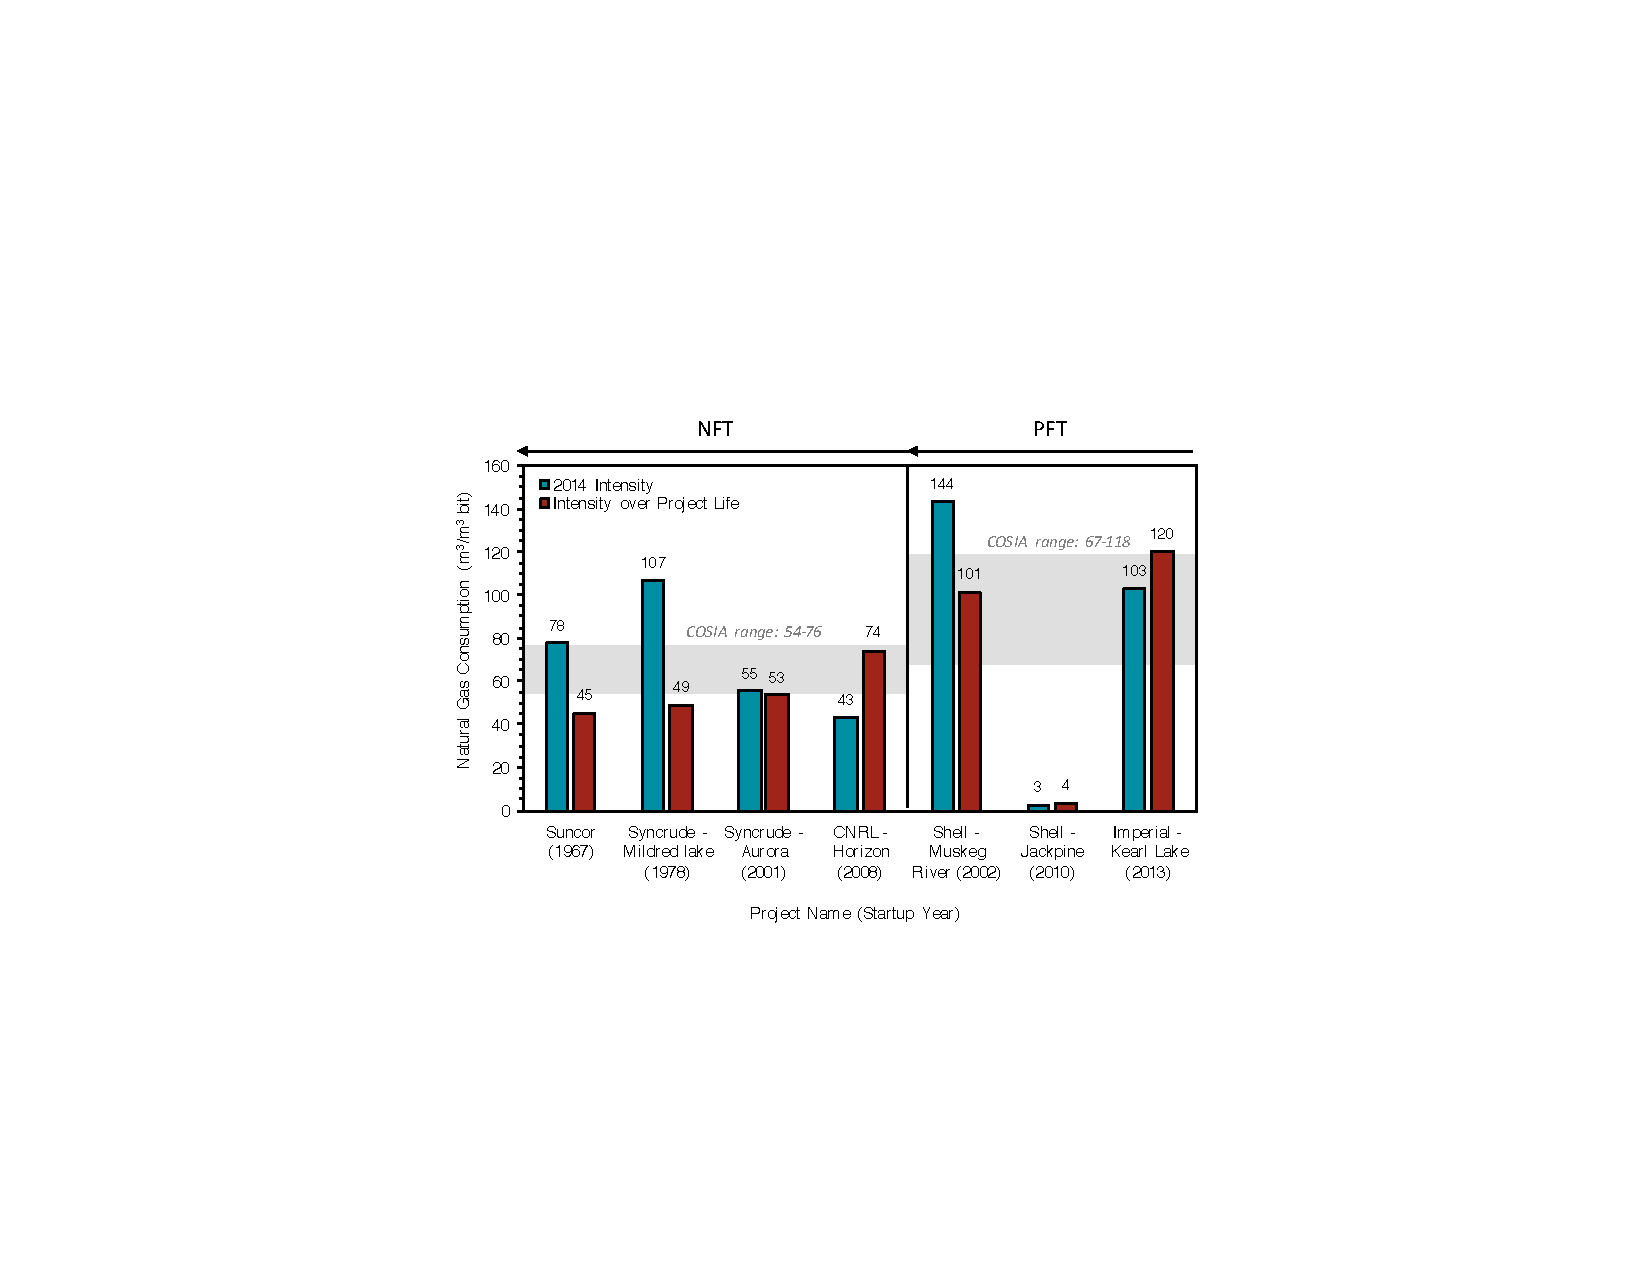
\includegraphics[width=1\columnwidth]{images/mining_ng.pdf}
\caption{Natural gas use in mining operations.}
\label{fig:mining_ng}
\end{figure}


\begin{figure}[t]
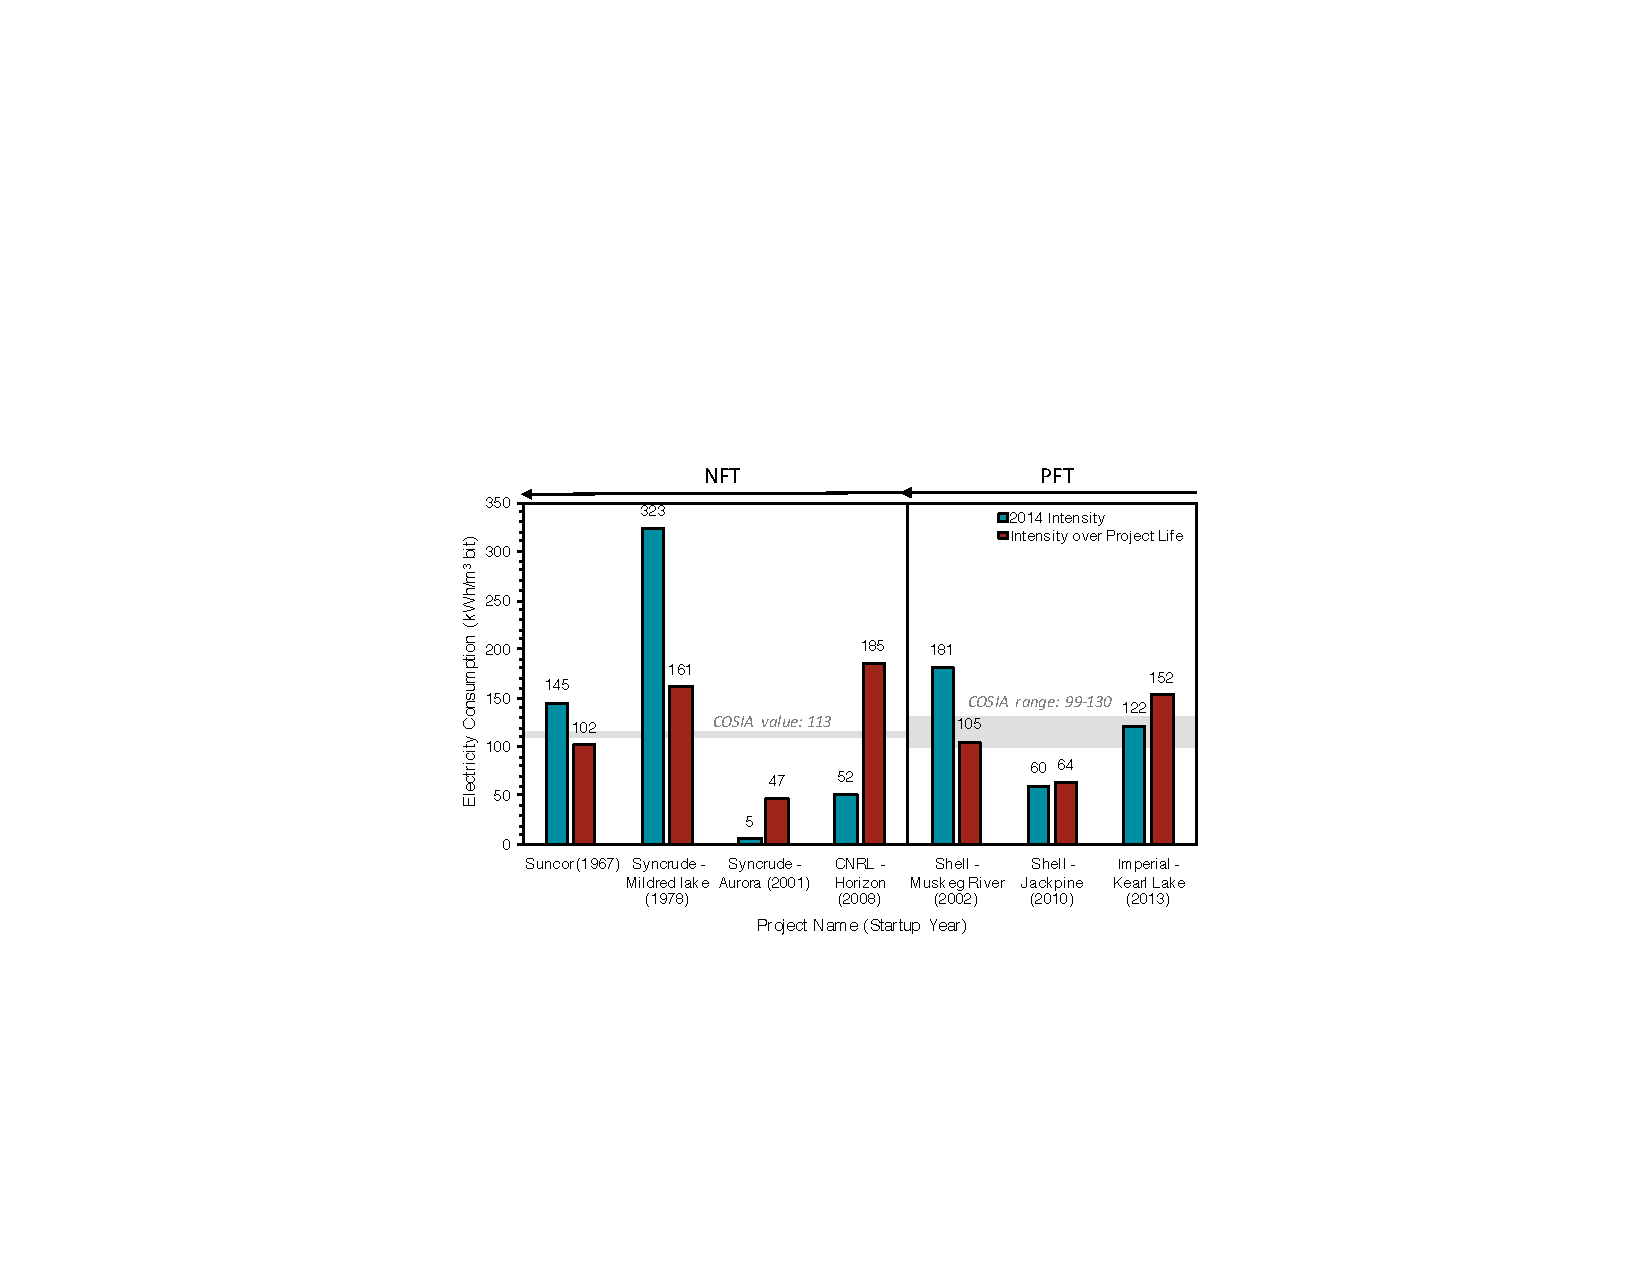
\includegraphics[width=1\columnwidth]{images/mining_elec.pdf}
\caption{Electricity use in mining operations.}
\label{fig:mining_elec}
\end{figure}

\paragraph{Modeling of non-integrated PFT mining operations}

The non-integrated mining operation is illustrated in Figure \ref{fig:pfd_mining_nint}.  The energy imports to the stand-alone mining operation include diesel imports, electricity imports, and natural gas imports. Some mining operations co-generate power on site and may also export power. The mine takes in raw bitumen ore and exports diluted bitumen for shipment to upgraders or direct shipment to refineries.

The default values for energy use in non-integrated PFT mining operations are computed as follows:
\begin{itemize}
\item Natural gas consumption is modeled using the AER 2014 production-weighted average for three stand-alone PFT projects (Shell Muskeg River, Shell Jackpine, and Imperial Kearl).
\item Electricity consumption is modeled using the AER 2014 production-weighted average for three stand-alone PFT projects (Shell Muskeg River, Shell Jackpine, and Imperial Kearl).
\item Diesel consumption is estimated as the average of COSIA reported high and low ranges of diesel consumption, as reported for low-grade (9 wt.\% and high-grade (12 wt.\%) ores respectively. The range from the COSIA templates is used as the range of diesel consumption rate.
\item Diluent blending rates are modeled using AER 2014 production-weighted averages from the stand-alone PFT projects (Shell Muskeg River, Shell Jackpine, and Imperial Kearl). Volumetric blending rates over all months averaged 25.4\% diluent in dilbit. The range over 2014 was from 24.3\% to 26.5\% Although Kearl dilutes bitumen with SCO (creating ``syn-bit'') the dilution fraction was nearly identical to those of Muskeg River and Jackpine.
\end{itemize}

Table \ref{tab:mining_nonint_energy} gives results as used in OPGEE, results for the AER production-weighted average, COSIA template average, and COSIA template range. SI units are presented at top of Table \ref{tab:mining_nonint_energy}, while OPGEE inputs are also converted below to the field units used in OPGEE for alignment with values in model.


\begin{table}
\caption{Non-integrated PFT mining energy intensities.}
\label{tab:mining_nonint_energy}
\begin{scriptsize}
\begin{tabularx}{1\columnwidth}{p{0.2\columnwidth}p{0.07\columnwidth}p{0.08\columnwidth}p{0.07\columnwidth}p{0.08\columnwidth} p{0.2\columnwidth}p{0.05\columnwidth}}
\toprule
Fuel & OPGEE value & AER PW avg. & COSIA avg. & COSIA range & Units &  Notes\\
\midrule
SI units 			&	& 	&	&			& &  \\
\midrule
Natural gas 		& 85 		& 85 		& 93 		& 67 -- 118		& m$^3$ gas / m$^3$ bitumen& \\
Electricity	cons.	& 125	& 125	& 114	& 99 -- 130		& kWh / m$^3$ bitumen &\\
Electricity gen.		& 77		& 77		& 114	& 96 -- 132		& kWh / m$^3$ bitumen  &\\
Frac. elect. gen. onsite	& 0.6 & 0.6	& 1.0		& 1.0 -- 1.0		& kWh/kWh & \\
Diesel			& 12.5	& -		& 12.5	& 9 -- 16			& L / m$^3$ bitumen & a \\	
Diluent			& 25.4\%	& 25.4\%	& -		& -				& vol. \% & \\
\midrule
OPGEE units 			&	& 	&	&			& &  \\
\midrule
Natural gas 		& 415		& -	& -		& -		& scf gas / bbl bitumen& \\
Electricity	cons.	& 19.9	& -	& -	& -		& kWh / bbl bitumen &\\
Electricity gen.		& 12.2		& -		& -	& -		& kWh / bbl bitumen  &\\
Frac. elect. gen. onsite	& 0.6 & -	& -		& -		& kWh/kWh & \\
Diesel			& 0.52 	& -		& -	& -			& gal. / bbl bitumen & a \\	
Diluent			& 25.4\%	& -	& -		& -				& vol. \% & \\
\bottomrule
\end{tabularx}
\begin{tablenotes}
\item[a] COSIA Mine Template ranges presented for low (9\%) and high (12\%) grade ore.
\end{tablenotes}
\end{scriptsize}
\end{table}

\paragraph{Proposed modeling of integrated NFT mining operations}


The integrated mining operation is illustrated in Figure \ref{fig:pfd_mining_int}.  The net flows across the process boundary are roughly equivalent to the stand-alone mining operation, with some exceptions. First, large volumes of diluent are not used to reduce the viscosity of bitumen, as upgrading the bitumen to SCO renders it ready for pipeline transport.  Also, two new co-products can be exported from the system: process gas and coke.  Therefore, emissions credits should be given for these fuels if they are exported.  Lastly, new internal flows between upgrader and mine include heat recovered from upgrader operations that is used in mine ore separations, as well as upgrader product streams (distillate fuels) that are consumed in mining trucks.  New internal consumption at the upgrader can include coke and process gas.

Due to sharing of waste heat at integrated mining and upgrading projects, some efficiency is gained through process integration.  Suncor and Jacobs (2012) estimate that 30 percent of total natural gas required at a project can be reduced by using low-grade waste heat from an integrated upgrader for the bitumen extraction process.

Updated OPGEE default values for stand-alone NFT mines are taken directly from the COSIA NFT Mine Template \cite{COSIA2015b}. The efficiency factor from Suncor and Jacobs \cite{Jacobs2012} is multiplied by the COSIA stand-alone mining natural gas consumption to approximate the natural gas consumed solely by the mine at an integrated mining and upgrading facility. These values are compared to the energy consumption for integrated mining and upgrading projects in Table \ref{tab:mining_comp_integration}. The remaining energy for integrated projects not attributed to mining is approximately that consumed in the upgrading process.  For example, if we compare Suncor and Syncrude natural gas consumption (total) less that estimated used in upgrading, we get values approximately equal to the COSIA stand-alone NFT mine less a 30\% integration benefit (40-45 m$^3$ per $m^3$) .  

\begin{landscape}
\begin{table}
\begin{scriptsize}
\tablefirsthead{\toprule Fuel & OPGEE value$^{a}$ & COSIA SA NFT$^{b}$ & AER reported$^{c}$ & & Upgrading est.$^{d}$ &  \\ \midrule}
\tabletail{\bottomrule \multicolumn{7}{p{1\columnwidth}}{\textit{Continued on next page...}}\\}
\tablelasttail{\bottomrule}
\tablecaption{Comparison between stand-alone mine energy consumption estimates based on COSIA mine template to integrated NFT mining and upgrading energy consumption reported by AER.}
\label{tab:mining_comp_integration}
\begin{threeparttable}
\begin{supertabular*}{1\columnwidth}{p{0.3\columnwidth}p{0.08\columnwidth}p{0.08\columnwidth}p{0.08\columnwidth}p{0.08\columnwidth} p{0.08\columnwidth}p{0.08\columnwidth}}
				&		&				& Suncor	& Syncrude	& Suncor	& Syncrude \\	
				\midrule
Natural gas cons. 
(m$^3$ gas/m$^3$ bitumen)	& 45		& 65 (54 -- 76)$^{e}$		& 78		& 77		&	30 	& 37  \\
Electricity	cons. (kWh/m$^3$ bitumen)	& 113	& 113			& 145	& 166		& 	30	& 63 \\
\end{supertabular*}
\begin{tablenotes}
\item[a] Natural gas consumption for mining portion of an integrated mining and upgrading project calculated by subtracting the percentage of natural gas Suncor and Jacobs \cite{Jacobs2012} estimate will be saved through sharing of waste heat. 
\item[b] Includes mining energy consumption estimates provided in COSIA Mine Templates for a representative stand-alone NFT mine.
\item[c] 2014 operating data reported in AER Statistical Report ST39. Suncor and Syncrude projects have on-site upgraders so AER data is reported for both mining and upgrading.
\item[d] Estimate of energy consumed from upgrading calculated by subtracting the estimated energy consumed for mining in integrated projects from the mining and upgrading energy consumption reported to the AER. The values presented in the table for upgrading are per m$^3$ of SCO produced by the on-site upgrader (17,200,000 m$^3$ and 15,200,000 m$^3$ for Suncor and Syncrude upgraders, respectively), whereas the energy consumption values for mined bitumen presented in the table are per m$^3$ of bitumen produced.
\item[e] The range presented in the table for natural gas consumption from the COSIA Mine Template for NFT projects is based on the low and high estimates for natural gas consumption for high grade and low grade oil sands ore, respectively. The same values for electricity consumption are reported for low and high grade ore in the NFT COSIA Mine Template (113 kWh/m$^3$ bitumen).
\end{tablenotes}
\end{threeparttable}
\end{scriptsize}
\end{table}
\end{landscape}


In order to enable self-consistent treatment of integrated mining and upgrading, the following conventions are applied:
\begin{itemize}
\item Integrated mining and upgrading operations use the same upgrading models described below in Section \ref{sec:upgrading}.
\item Any benefits associated with upgrading integration result in less net consumption of mining consumables that flow across conventional mine boundary (i.e., diesel, electricity, natural gas).
\item Emissions associated with on-site use of fuels by upgrader are calculated on the upgrading sheet.
\end{itemize}
These conventions allow for computation of the benefits of integrated mining and upgrading operations, while also maintaining computations of emissions impacts of operations.

The default values for energy use in upgrader-integrated NFT mining operations are therefore computed as follows:
\begin{itemize}
\item Natural gas consumption is modeled using COSIA stand-alone NFT mine less a 30\% integration benefit. This is approximately equal to the reported values of Suncor and Syncrude less estimated upgrading consumption.
\item Electricity consumption is modeled using COSIA electricity use at a stand-alone NFT mine.  No integration benefit applicable.
\item Diesel consumption is estimated as the average of COSIA reported high and low ranges of diesel consumption, as reported for low-grade (9 wt.\% and high-grade (12 wt.\%) ores respectively.
\end{itemize}



\begin{table}
\begin{scriptsize}
\tablefirsthead{\toprule Fuel & OPGEE value & AER PW avg. & COSIA avg. & COSIA range & Units & Notes\\
\midrule}
\tablehead{ \multicolumn{7}{p{1\columnwidth}}{\textit{Continued from previous page}}\\ \toprule Fuel & AER prod-weighted avg. & COSIA avg. & COSIA range & Units & Notes \\ 
\midrule }
\tabletail{\bottomrule \multicolumn{7}{p{1\columnwidth}}{\textit{Continued on next page...}}\\}
\tablelasttail{\bottomrule}
\tablecaption{Integrated NFT mining energy intensities.}
\label{tab:mining_int_energy}
\begin{threeparttable}[t]
\begin{supertabular*}{1\columnwidth}{p{0.2\columnwidth}p{0.08\columnwidth}p{0.08\columnwidth}p{0.08\columnwidth}p{0.08\columnwidth} p{0.2\columnwidth}p{0.05\columnwidth}}
SI units			&		&		&		&			&						& \\
\midrule
Natural gas		& 45		& -		& 65		& 54 -- 76		& m$^3$ gas / m$^3$ bitumen  	&$a$\\
Electricity	cons.	& 113	& -		& 113	& 113 -- 113	& kWh / m$^3$ bitumen	& \\
Electricity gen.		& 114	& -		& 114	& 96 -- 132	& kWh / m$^3$ bitumen	& \\
Frac. elect. gen. onsite	& 1 	& -		& 1.0 	& 0.8-- 1.2		& kWh/kWh	& \\
Diesel			& 11		& -		& 11		& 9 -- 13		& L / m$^3$ bitumen	& $b$ \\	
\midrule
OPGEE units			&		&		&		&			&						& \\
\midrule
Natural gas		& 304		& -		& -		&-		& scf gas / bbl bitumen  	&$a$\\
Electricity	cons.	& 18.0	& -		& -	& -	& kWh / bbl bitumen	& \\
Electricity gen.		& 18.1	& -		& -	&-	& kWh / bbl bitumen	& \\
Frac. elect. gen. onsite	& 1 	& -		& - 	& -		& kWh/kWh	& \\
Diesel			& 0.46		& -		& -		&-		& gal / bbl bitumen	& $b$ \\	
\end{supertabular*}
\begin{tablenotes}
\item[a] Note from Table \ref{tab:mining_comp_integration} above that the COSIA stand-alone NFT mine consumption must be reduced by the heat integration benefit. That is, OPGEE value of 45 m$^3$ per m$^3$ bitumen should be compared to 65$\times (1.0-0.3)$) \cite{COSIA2015b}
\item[b] COSIA Mine Template ranges presented for low (9\%) and high (12\%) grade ore.
\end{tablenotes}
\end{threeparttable}
\end{scriptsize}
\end{table}


\begin{figure}[t]
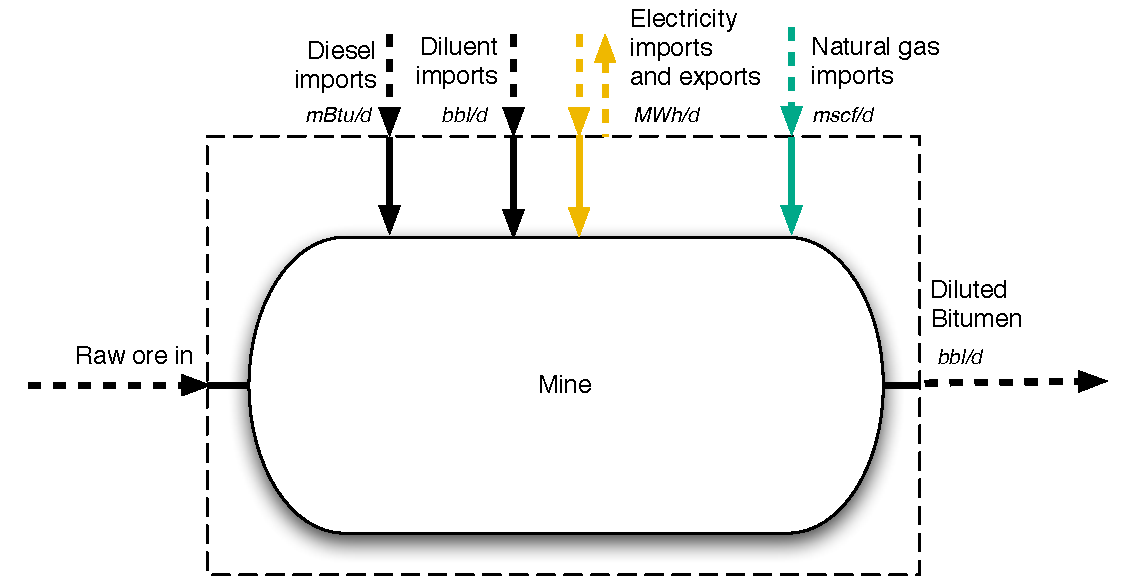
\includegraphics[width=0.9\columnwidth]{images/Mining_NInt.pdf}
\caption{Non-integrated bitumen mining operation.}
\label{fig:pfd_mining_nint}
\end{figure}


\begin{figure}[t]
\includegraphics[width=1\columnwidth]{images/Mining_Int.pdf}
\caption{Upgrader-integrated bitumen mining operation}
\label{fig:pfd_mining_int}
\end{figure}

For both integrated and non-integrated mining operations, the emissions and energy use are tracked simply.  For example, diesel fuel use in non-integrated mining operations is computed as:
\begin{equation}\label{eq:dieselmine}
Q_{di}^{MN} = Q_{db}^{MN} I_{di}^{MN} \quad\quad\eqnunitfrac{gal}{d}
\end{equation}
where $Q_{di}^{MN}$ is diesel consumed in non-integrated mining operations [gal/d], $Q_{db}^{MN}$ is diluted bitumen output from the non-integrated mining operation [bbl/d], and $I_{di}^{MN}$ is the diesel fuel intensity of non-integrated mining operations [gal/bbl].  This quantity of diesel fuel consumed can then be converted into an energy consumption rate:
\begin{equation}
E_{di}^{MN} = Q_{di}^{MN} LHV_{di} \quad\quad\eqnunitfrac{mBtu LHV}{gal}
\end{equation}
where $LHV_{di}$ is the lower heating value of diesel fuel [mBtu LHV/gallon].  This quantity can then be gathered on the \sheet{Energy Summary} gathering sheet and used to compute emissions on the \sheet{GHG Summary} gathering sheet.

Similar quantities are computed for all main inputs to non-integrated mining operations by using intensities of electricity use ($I_{el}^{MN}$) and natural gas ($I_{ng}^{MN}$).  For the case of integrated mining and upgrading operations, the relevant intensities for diesel, electricity, and natural gas are similarly named ($I_{di}^{MI}$, $I_{el}^{MI}$, and $I_{ng}^{MI}$ respectively). Recall via convention above that consumption of coke or refinery process gas is computed as part of upgrading operations in Section \ref{sec:upgrading}.

After these mine-type-specific calculations are performed, the overall consumption due to mining is then computed using binary variables from the \sheet{Active Field} sheet. For the case of diesel energy consumption:

\begin{minipage}{0.6\columnwidth}
\begin{fleqn}[0pt]
\begin{equation}\label{eq:minesum}
E_{di} = y^{MN}E_{di}^{MN}  + y^{MI}E_{di}^{MI} \quad\quad\eqnunitfrac{mBtu LHV}{gal}
\end{equation}
\end{fleqn}
\end{minipage}\hfill
\begin{minipage}{0.3\columnwidth}
        \begin{tabular}{|cl}
                        & \\
        $y^{MN}$       & \xlname{Oil\_sands\_mine\_int\_01}\\
        $y^{MI}$        & \xlname{Oil\_sands\_mine\_nonint\_01}\\
        & \\
        \end{tabular}
\end{minipage}

where $y^{MN}$ and $y^{MI}$ represent binary variables for mining-non-integrated and mining-integrated, respectively.

\subsection{Defaults for bitumen mining}

Default values for bitumen mining calculations are shown in Tables \ref{tab:primary_inputs_mining} and \ref{tab:secondary_inputs_mining}.

\begin{landscape}

\begin{tiny}
\tablefirsthead{\toprule Param. & Description & Defined name & Default & Literature range & Unit & Sources & Notes\\
\midrule}
\tablehead{ \multicolumn{8}{p{1\columnwidth}}{\textit{Continued from previous page}}\\ \toprule Param. &Description & Defined name &Default & Literature range & Unit & Sources & Notes \\ 
\midrule }
\tabletail{\bottomrule \multicolumn{8}{p{1\columnwidth}}{\textit{Continued on next page...}}\\}
\tablelasttail{\bottomrule}
\tablecaption{Primary inputs used in \sheet{Bitumen mining} sheet.}
\label{tab:primary_inputs_mining}
\begin{threeparttable}
\begin{supertabular*}{1\columnwidth}{p{0.03\columnwidth}p{0.3\columnwidth}p{0.25\columnwidth}p{0.05\columnwidth}p{0.05\columnwidth}p{0.05\columnwidth}p{0.025\columnwidth}p{0.025\columnwidth}}
$Q_0$ & Oil production volume & \xlname{Oil\_prod} & 1,500 & 10-3,000,000 & [bbl/d] & & \\  
$y_{OS,mi}$     & Oil sands mine integrated with upgrader?  & \xlname{Oil\_sands\_mine\_int\_01} & 0 & 0-1 & [binary 0-1] & & \\
$y_{OS,mn}$     & Oil sands mine non-integrated with upgrader?  & \xlname{Oil\_sands\_mine\_nonint\_01} & 0 & 0-1 & [binary 0-1] & & \\
$FOR$     & Ratio of flaring to oil production  & \xlname{FOR} & var. & var.  & [scf/bbl] & & \\
$VOR$     & Ratio of venting to oil production  & \xlname{VOR} & var. & 0  & [scf/bbl] & & \\
$x_{N_2}$     & Nitrogen gas composition & \xlname{Gas\_comp\_N2} & 2 & var. & mol\% & & \\
$x_{CO_2}$     & CO$_2$ gas composition & \xlname{Gas\_comp\_CO2} & 6 & var. & mol\% & & \\
$x_{C_1}$     & Methane gas composition & \xlname{Gas\_comp\_C1} & 84 & var. & mol\% & & \\
$x_{C_2}$     & Ethane gas composition & \xlname{Gas\_comp\_C2} & 4 & var. & mol\% & & \\
$x_{C_3}$     & Propane gas composition & \xlname{Gas\_comp\_C3} & 2 & var. & mol\% & & \\
$x_{C_{4}+}$     & C$_4$+ gas composition & \xlname{Gas\_comp\_C4} & 1 & var. & mol\% & & \\
$x_{H_{2}S}$     & H$_2$S gas composition & \xlname{Gas\_comp\_H2S} & 1 & var. & mol\% & & \\

\end{supertabular*}
%\begin{tablenotes}
%\item[a] Insert text of note here
%\end{tablenotes}
\end{threeparttable}
\end{tiny}

\newpage

\begin{tiny}
\tablefirsthead{\toprule Param. & Description & Defined name & Default & Literature range & Unit & Sources & Notes\\
\midrule}
\tablehead{ \multicolumn{8}{p{1\columnwidth}}{\textit{Continued from previous page}}\\ \toprule Param. &Description & Defined name &Default & Literature range & Unit & Sources & Notes \\ 
\midrule }
\tabletail{\bottomrule \multicolumn{8}{p{1\columnwidth}}{\textit{Continued on next page...}}\\}
\tablelasttail{\bottomrule}
\tablecaption{Secondary inputs used in \sheet{Bitumen mining} sheet.}
\label{tab:secondary_inputs_mining}
\begin{threeparttable}
\begin{supertabular*}{1\columnwidth}{p{0.03\columnwidth}p{0.3\columnwidth}p{0.25\columnwidth}p{0.05\columnwidth}p{0.05\columnwidth}p{0.05\columnwidth}p{0.05\columnwidth}p{0.025\columnwidth}}
$T_{mined,b}$        & Mined bitumen temperature                                	& \xlname{Temperature\_mined\_bitumen} 			& 80					& 				& [$^\circ$F] 		& Assumption &  \\
$p_{mined,b}$        & Mined bitumen pressure                                		& \xlname{Pressure\_mined\_bitumen} 				& 14.7				& 				& psia 			& Assumption &   \\
$\Gamma_{b}$        	& Crude bitumen specific gravity                                & \xlname{API\_bitumen} 							& 8	 				& 2-60 			& [$^\circ$API]  	& Assumption &   \\
        	$f_{g,con.}$ 			& Fraction of gas consumed in equip.                          & \xlname{Fraction\_natural\_equip\_mined\_bitumen} 	& [binary 0-1]	 		& 				&   				& Assumption &    \\

\end{supertabular*}
%\begin{tablenotes}
%\item[a] Insert text of note here
%\end{tablenotes}
\end{threeparttable}
\end{tiny}


\end{landscape}

\clearpage


%%%%%%%%%%%%%%%%%%%%%%%%%%%%
\section{Separation}
\label{sec:Separation}

The streams flowing into and out of the separation process are shown in Figure \ref{fig:separation_PF} and are listed in Table \ref{tab:separation_PF}.

The separation process assumes horizontal 3-phase separators, high pressure. Custom separation equipment, such as for offshore facilities, are not modeled in detail. 

Package-built separator specifications are collected from a surface processing supplier \cite{Surfaceequip2014}, for working pressures of 720, 1,000, 1,200, and 1,440 psig. The liquid capacity and gas processing capacity as a function of pressure are tabulated. The nearest effective wellhead pressure is chosen by selecting the first working pressure that is greater than or equal to the actual wellhead pressure. 

The total liquid production rate is given as $Q_o(1+F_{wo})$ \unit{bbl}{d}. Given the liquid treating capacity of each unit, we compute the number of each type of valid separator needed. The type of separator with the fewest required separators is chosen as the type to purchase. Given that liquid treating volume, the potential gas throughput is computed at the working pressure of the separator, and a check ensures whether there are enough separators to process the gas.

For simplicity, the separator gas specific gravity (\xlname{INDEX(FlowTable,GAMMA\_G,28)}) and heating value (\xlname{INDEX(FlowTable,LHV\_G\_scf,28)}) are assumed constant for all phases of separator. The separator gas specific gravity is defined as a working parameter \xlname{Gas\_sg} for ease of use in later formulas.  

Each stage of separation is assumed to occur at a pressure specified in the \sheet{Secondary Inputs} sheet. These are defined as \xlname{Pressure\_first\_separator}, \xlname{Pressure\_second\_separator}, and \xlname{Pressure\_third\_separator}. The defined function \xlname{SolutionGasOilRatio} is used to determine the solution gas oil ratio $R_s$ (see Eq. \ref{eq:GOR_OS}). 

The free gas removed by the the first stage of separation is defined as:

\begin{minipage}{0.6\columnwidth}
\begin{fleqn}[0pt]
\begin{equation} \label{eq:free_gas_separator}
R_{F,1} =  GOR - R_{s,1} \quad\quad\eqnunitfrac{scf}{bbl}
\end{equation}
\end{fleqn}
\end{minipage}\hfill
\begin{minipage}{0.3\columnwidth}
        \begin{tabular}{|cl}
                &    \\
                    $GOR$         & \xlname{GOR}     \\
                    $R_{s,1}$   & \xlname{SolutionGasOilRatio(x,1)} \\
               &    \\
        \end{tabular}
\end{minipage}

where \xlname{SolutionGasOilRatio} is the user-defined Excel function that computes the quantity of gas in solution at a given temperature, pressure, and given crude oil and gas gravities. The solution gas oil ratio custom function is described in detail above in the section on flow sheet calculations and shown in equation \ref{eq:GOR_OS}.

$R_{s,1}$ is the solution gas oil ratio $R_s$ with first-stage separation conditions (temperatures and pressures) plugged in. Similarly, the free gas removed by the second stage $R_{F,1}$ is equal to the gas in solution after stage 1 less the gas in solution after stage 2: $R_{s,1} - R_{s,2}$

The oil FVF at each stage, accounting for gas no longer in solution, is computing using the methods outlined above in the flow sheet description, starting in Eq. \ref{eq:BOB}. The oil specific gravity at each stage is computed using the methods outlined in Eq. \ref{eq:rho_o}, given the varying amount of gas in solution at that stage.

The compression ratio for each stage is computed as the ratio of the outlet gas pressure \xlname{INDEX(FlowTable,P,28)} from the entire separation process to the stage operating pressure. Once the compression ratio is computed, the compressor work and energy consumption computation methods are used for as for individual compressors. See Section \ref{sec:gas_reinjection_compressor} below for a detailed discussion of compressor energy use and emissions calculation. 

\subsection{Defaults for separation}

Default values for separation calculations are shown in Tables \ref{tab:primary_inputs_separation}, and \ref{tab:secondary_inputs_separation}.

\clearpage

%%%%%%%%%%%
\begin{table}
\caption{Streams flowing into and out of the separation process. I/O denotes input or output stream.}
\label{tab:separation_PF}
\begin{scriptsize}
\begin{tabularx}{1\columnwidth}{p{0.32\columnwidth}p{0.05\columnwidth}p{0.04\columnwidth}p{0.32\columnwidth}p{0.05\columnwidth}p{0.05\columnwidth}}
\toprule
Flow name							& Stream   			& I/O 	& Source/Destination       			& Units 			&  Notes\\ 
\midrule
Oil at wellhead							& \stream{4}			& I		& Wellbore/downhole pump		& [t/d]			&			\\
Water at wellhead						& \stream{102}			& I		& Wellbore/downhole pump		& [t/d]			&			\\
Gas at wellhead						& \stream{27}			& I		& Wellbore/downhole pump		& [t/d]			&			\\
\midrule
Oil after separator						& \stream{7}			& O		& Crude oil dewatering			& [t/d]			&			\\
Water after separator 					& \stream{103}			& O		& Produced water treatment		& [t/d]			&			\\
Gas after separator						& \stream{28}			& O		& Flaring						& [t/d]			&			\\
Separator leaks to air					& \stream{251}			& O		& Environment - Atmosphere		& [t/d]			&			\\	
\bottomrule
\end{tabularx}
\end{scriptsize}
\end{table}
%%%%%%%%%%%


%%%%%%%%%%%
\begin{figure}
\includegraphics[width=0.85\columnwidth]{images/Separation_PF.pdf}
\caption{Streams flowing into and out of the separation process. All streams measured in tonnes per day excepting electricity which is measured in MWh/d.}
\label{fig:separation_PF}
\end{figure}
%%%%%%%%%%%




\begin{landscape}

\begin{tiny}
\tablefirsthead{\toprule Param. & Description & Defined name & Default & Literature range & Unit & Sources & Notes\\
\midrule}
\tablehead{ \multicolumn{8}{p{1\columnwidth}}{\textit{Continued from previous page}}\\ \toprule Param. &Description & Defined name &Default & Literature range & Unit & Sources & Notes \\ 
\midrule }
\tabletail{\bottomrule \multicolumn{8}{p{1\columnwidth}}{\textit{Continued on next page...}}\\}
\tablelasttail{\bottomrule}
\tablecaption{Primary inputs used in \sheet{Separation} sheet.}
\label{tab:primary_inputs_separation}
\begin{threeparttable}
\begin{supertabular*}{1\columnwidth}{p{0.03\columnwidth}p{0.25\columnwidth}p{0.25\columnwidth}p{0.07\columnwidth}p{0.07\columnwidth}p{0.07\columnwidth}p{0.07\columnwidth}p{0.07\columnwidth}}
$WOR$        & Water oil ratio                   & \xlname{WOR} & 8     & 1-10,000   & [-] & & \\
$Q_o$           & Production rate of oil            & \xlname{Oil\_prod}    & 1,500     & 10-3,000,000  & [bbl/d] & & \\
$GOR$          & Gas oil ratio, producing          & \xlname{GOR}          & var.      & 5-100,000     & [scf/bbl] & & \\
$x_{a}$         & Mole fraction of species $a$ in gas   & \xlname{Gas\_comp\_a}     & var.      & 5-100,000     & [scf/bbl] & & \\ 
\end{supertabular*}
%\begin{tablenotes}
%\item[a] Insert text of note here
%\end{tablenotes}
\end{threeparttable}
\end{tiny}

\newpage

\begin{tiny}
\tablefirsthead{\toprule Param. & Description & Defined name & Default & Literature range & Unit & Sources & Notes\\
\midrule}
\tablehead{ \multicolumn{8}{p{1\columnwidth}}{\textit{Continued from previous page}}\\ \toprule Param. &Description & Defined name &Default & Literature range & Unit & Sources & Notes \\ 
\midrule }
\tabletail{\bottomrule \multicolumn{8}{p{1\columnwidth}}{\textit{Continued on next page...}}\\}
\tablelasttail{\bottomrule}
\tablecaption{Secondary inputs used in \sheet{Separation} sheet.}
\label{tab:secondary_inputs_separation}
\begin{threeparttable}
\begin{supertabular*}{1\columnwidth}{p{0.03\columnwidth}p{0.25\columnwidth}p{0.25\columnwidth}p{0.07\columnwidth}p{0.07\columnwidth}p{0.07\columnwidth}p{0.07\columnwidth}p{0.07\columnwidth}}
$C_{cm,sp}$    & Choice of separation compressor prime mover type       & \xlname{Prime\_mover\_type\_separator\_compressor} &   2 & 1 or 2  & [-] &  & $a$ \\
$f_{w,e}$        & Mass fraction water in emulsion after separation     & \xlname{Water\_content\_oil\_emulsion} & 14 & 0-20 & [wt\%] & & \\
$n_{sp}$        & Number of separation stages                    & \xlname{Number\_stages\_separator}  & 3 & 1-3 & - & & \\
$p_{sp,1st}$       & First stage separator pressure                       & \xlname{Pressure\_first\_separator} & 1000 & 50-2000  & [psig] & & \\
$p_{sp,2nd}$       & Second stage separator pressure                       & \xlname{Pressure\_second\_separator} & 575 & 50-2000  & [psig] & & \\
$p_{sp,3rd}$       & Third stage separator pressure                       & \xlname{Pressure\_third\_separator} & 150 & 50-2000  & [psig] & & \\
$p_{sp,f}$       & Final stage separator pressure                       & \xlname{Pressure\_outlet\_separator} & 150 & 50-2000  & [psig] & & \\
$p_{l}$         & Line-specification pressure to leave separation       & \xlname{Pressure\_after\_boosting\_separator} & 1000 & 50-2000  & [psig] & & \\
$T_{sp}$        & Separator temperature, final                          & \xlname{Temperature\_outlet\_separator} & 90 & 50-200 & [$^\circ$] & & \\
$\eta_{cm,sp}$   & Efficiency of separation compressors             & \xlname{Eta\_compressor\_separation}  & 75    & 60-80 & [\%] & & \\
\end{supertabular*}
\begin{tablenotes}
\item[a] Type 1 is electric motor, Type 2 is NG engine
\end{tablenotes}
\end{threeparttable}
\end{tiny}

\end{landscape}


\clearpage





%%%%%%%%%%%%%%%%%%%%%%%%%%%%
\section{Crude oil dewatering}
\label{sec:Dewatering}

Removing free water from crude oil can be accomplished by passive chemical and gravitational methods that do not use heat. Because no fuel is used in passive gravitational separation techniques, they do not cause significant GHG emissions. However, based on the properties of the oil, gravity separation techniques may not be sufficient to produce crude oil with the desired water content required for transport and sales. Additional separation may be provided by a crude oil heater-treater, which may be turned ON or OFF in OPGEE, \xlname{Heater\_treater} to remove entrained water remaining after passive separation. 

The streams flowing into and out of the \sheet{Crude oil dewatering} sheet are shown in Figure \ref{fig:crude_oil_dewatering_PF} and are listed in Table \ref{tab:crude_oil_dewatering_PF}.

First the average crude oil temperature during heating is computed:

\begin{minipage}{0.6\columnwidth}
\begin{fleqn}[0pt]
\begin{equation} \label{eq:temp_dewater}
T_{dw,avg} =  \frac{T_{\mstream{7}} + T_{dw}}{2} \quad\quad\eqnunit{$^\circ$F} 
\end{equation}
\end{fleqn}
\end{minipage}\hfill
\begin{minipage}{0.3\columnwidth}
        \begin{tabular}{|cl}
        & \\
                    $T_{\mstream{7}}$    & \xlname{INDEX(FlowTable,T,7)}     \\
                    $T_{dw}$   & \xlname{Temperature\_heater\_treater} \\
                     & \\
        \end{tabular}
\end{minipage}

Default values are 165 $^{\circ}${F} for watering temperature $T_{dw}$. 

The specific heat capacity of oil is a function of the temperature of the oil and its API gravity. From the Campbell equation, presented in Manning and Thompson \cite{Manning1991}:

\begin{minipage}{0.8\columnwidth}
\begin{fleqn}[0pt]
\begin{equation} \label{eq:CampbellCpOil}
C_{p,o} = a_1 T_{dw,avg} API_o + a_2 API_o + a_3 T_{dw,avg} + a_4 \quad\quad\eqnunitfrac{Btu}{lb-$^\circ$F}
\end{equation}
\end{fleqn}
\end{minipage}\hfill
\begin{minipage}{0.3\columnwidth}
        \begin{tabular}{|cl}
         & \\
                    $a_1 \ldots a_4$ & \xlname{O\_Cp\_a1}     \\
                    $API_{o}$   & \xlname{API} \\
                     & \\
        \end{tabular}
\end{minipage}

To model heat capacity differences between water and oil \cite[p. 303]{Manning1995}, OPGEE assumes that oil entering a heater-treater contains only entrained water. The free water proportion that was not separated prior to the application of heat is assumed to be negligible (1-2\%)  \cite[Section 5.4.2]{Abdelaal2003}. 

The mass flow of incoming oil and water are given by the constituents of Stream \stream{7} which leaves the separator: $m_{\mstream{7},o}$ and $m_{\mstream{7},w}$. The enthalpy change required is calculated using:
%%%%%%%%%%
\begin{equation} \label{eq:crude_dehyd_heat}
\Delta H_{HT}= \Delta T_{HT} \left( m_{\mstream{7},o} C_{p_{o}} + m_{\mstream{7},w} C_{p_{w}} \right) (1+\epsilon_{HT}) \left( \frac{1}{10^6} \right) \quad\quad\eqnunitfrac{mmBtu}{d}
\end{equation}
%%%%%%%%%%
where $\Delta H_{CD}$ = heat duty [mmBtu/d]; $C_{p_{o}}$ = specific heat of oil [Btu/lb-$^{\circ}${F}]; $C_{p_{w}}$ = specific heat of water [Btu/lb-$^{\circ}${F}]; and $\epsilon_{CD}$ = heat loss [fraction]. The heat capacity of water is 1 Btu/lb-$^{\circ}${F}; and 0.02 for heat loss \cite[p. 136 and 303]{Manning1995}. Lastly, the enthalpy change of the fluids is multiplied by an efficiency factor:
%%%%%%%%%%
\begin{equation} \label{eq:EHT}
E_{HT} = \Delta H_{HT} \times \eta_{HT}  \quad\quad\eqnunitfrac{mmBtu}{d}
\end{equation}
%%%%%%%%%%

\subsection{Defaults for crude oil dewatering}

Default values for crude oil dewatering calculations is shown in Table \ref{tab:secondary_inputs_dewatering}.



\clearpage

%%%%%%%%%%%
\begin{table}
\caption{Streams flowing into and out of the crude oil dewatering process. I/O denotes input or output stream.}
\label{tab:crude_oil_dewatering_PF}
\begin{scriptsize}
\begin{tabularx}{1\columnwidth}{p{0.32\columnwidth}p{0.05\columnwidth}p{0.04\columnwidth}p{0.32\columnwidth}p{0.05\columnwidth}p{0.05\columnwidth}}
\toprule
Flow name							& Stream   			& I/O 	& Source/Destination       			& Units 			&  Notes\\ 
\midrule
Oil after separator						& \stream{7}			& I		& Separation					& [t/d]			&			\\
Fuel gas - Dewatering					& \stream{160}			& I		& Fuel gas system				& [t/d]			&			\\
Electricity - Dewatering					& \stream{184}			& I		& Electricity generation and imports	& [MWh/d]			&			\\
\midrule
Crude to stabilizer						& \stream{8}			& O		& Stabilizer					& [t/d]			&			\\
Crude to storage		 				& \stream{9}			& O		& Crude oil storage				& [t/d]			&			\\
Crude to upgrading						& \stream{19}			& O		& Heavy oil upgrading			& [t/d]			&			\\
Crude to dilution						& \stream{20}			& O		& Heavy oil dilution				& [t/d]			&			\\	
Water from dewatering					& \stream{115}			& O		& Produced water treatment		& [t/d]			&			\\
\bottomrule
\end{tabularx}
\end{scriptsize}
\end{table}
%%%%%%%%%%%


%%%%%%%%%%%
\begin{figure}
\includegraphics[width=0.85\columnwidth]{images/Crude_oil_dewatering_PF.pdf}
\caption{Streams flowing into and out of the crude oil dewatering process. All streams measured in tonnes per day excepting electricity which is measured in MWh/d.}
\label{fig:crude_oil_dewatering_PF}
\end{figure}
%%%%%%%%%%%


\begin{landscape}

\begin{tiny}
\tablefirsthead{\toprule Param. & Description & Defined name & Default & Literature range & Unit & Sources & Notes\\
\midrule}
\tablehead{ \multicolumn{8}{p{1\columnwidth}}{\textit{Continued from previous page}}\\ \toprule Param. &Description & Defined name &Default & Literature range & Unit & Sources & Notes \\ 
\midrule }
\tabletail{\bottomrule \multicolumn{8}{p{1\columnwidth}}{\textit{Continued on next page...}}\\}
\tablelasttail{\bottomrule}
\tablecaption{Secondary inputs used in \sheet{Crude oil dewatering} sheet.}
\label{tab:secondary_inputs_dewatering}
\begin{threeparttable}
\begin{supertabular*}{1\columnwidth}{p{0.03\columnwidth}p{0.25\columnwidth}p{0.25\columnwidth}p{0.07\columnwidth}p{0.07\columnwidth}p{0.07\columnwidth}p{0.07\columnwidth}p{0.07\columnwidth}}
$T_{dw}$    & Dewatering temperature	& \xlname{Temperature\_heater\_treater}		& 165	& 150-240	    & [$^\circ$F]	& \cite{Manning1991}		& -			\\
$\epsilon_{dw}$ & Heat loss				 & \xlname{Heat\_loss\_heater\_treater}	        & 2		& 1-3			& [\%] 		& \cite{Manning1991}		& -			\\
$y_{dw}$        & Type of heater		& \xlname{Type\_heater\_treater}	        & ``gas''	& ``gas'' or ``elec'' & [option]		& Assumption			& a			\\
$\eta_{dw,ng}$  & Heater fuel use factor	& \xlname{Eta\_heater\_treater\_gas}	& 0.8	& 0.7-0.85	        & [Btu/Btu]		& \cite{EPA2008}	    & -			\\
$\eta_{dw,e-}$  & Heater fuel use factor	& \xlname{Eta\_heater\_treater\_electric}	& 0.23	& 0.2-0.25		& [kWh/Btu]		& \cite{EPA2008}		& -			\\
\end{supertabular*}
\begin{tablenotes}
\item[a] ``Gas'' for natural gas fired heater, ``Elec'' for electric
\end{tablenotes}
\end{threeparttable}
\end{tiny}

\end{landscape}



\clearpage





%%%%%%%%%%%%%%%%%%%%%%%%%%%%%%%
\section{Crude oil stabilization}
\label{sec:crude_stabilization}

Following the removal of water content, stabilization is the next phase of the bulk separation process, and is most commonly applied to gas-rich light crude. Stabilization involves the forced removal of additional dissolved light hydrocarbons, beyond those removed during separation \cite[p. 159]{Manning1995}. Stabilization allows volatile light crudes to meet crude vapor pressure requirements for safety and environmental compliance.

The streams flowing into and out of the crude oil stabilization process are shown in Figure \ref{fig:crude_oil_stabilization_PF} and are listed in Table \ref{tab:crude_oil_stabilization_PF}.

The default type of stabilizer in OPGEE is a high-pressure stabilizer (100 psi) which requires a higher reboiler temperature than a low-pressure stabilizer. The use of a stabilizer column is an important assumption because a heat source is required to provide the required temperature. OPGEE assumes a direct-fired heater. 

The stabilizer column heat duty is calculated as:

\begin{minipage}{0.7\columnwidth}
\begin{fleqn}[0pt]
\begin{equation}  \label{eq:crude_stabilizer_heat}
\Delta H_{S}= \Delta T_{S} m_{\mstream{8},o} C_{p,o} \left(1+\epsilon_{S} \right) \left(\frac{1}{10^6} \right) \quad\quad\eqnunitfrac{mmBtu}{d}
\end{equation}
\end{fleqn}
\end{minipage}\hfill
\begin{minipage}{0.3\columnwidth}
        \begin{tabular}{|cl}
             &     \\
                    $T_S$       & \xlname{T\_S}     \\
                    $\epsilon_{S}$   & \xlname{EPS\_S} \\
                         &     \\
        \end{tabular}
\end{minipage}

where $\Delta H_{S}$ = heat duty [mmBtu/d]; $\Delta T_{S}$ = difference between reboiler and feed temperatures ($T_S - T_{\mstream{8},o}$) [$^{\circ}${F}]; $m_{\mstream{8},o}$ is the mass of oil flowing into the stabilizer as stream \stream{8} [lb/d]; $C_{p_{o}}$ = specific heat capacity of oil [Btu/lb-$^{\circ}${F}]; ; and $\epsilon_S$ = heat loss [fraction]. The default stabilizer temperature is 344 $^{\circ}${F} for the reboiler. 

The specific heat capacity of oil is calculated using the Campbell equation \cite{Manning1991}, shown above in Eq. \ref{eq:CampbellCpOil}. 

Fractional heat loss is 0.02 or 2\% of the heat load \cite[p. 136, 161, 163]{Manning1995} and boiler energy consumption to enthalpy ratio is 1.25 for natural gas and 0.37 kWh/Btu for electricity. 

The amount of gas evolved in the stabilizer is calculated as the difference between the solution gas oil ratio at the inlet pressure and temperature and at the outlet pressure and temperature using the equation of Al-Shammasi, described above in Eq. \ref{eq:GOR_OS}.

\subsection{Defaults for well and downhole pump}

Default values for reservoir calculations are shown in Table \ref{tab:secondary_inputs_stabilization}.

\clearpage


%%%%%%%%%%%
\begin{table}
\caption{Streams flowing into and out of the \sheet{Crude oil stabilization} process. I/O denotes input or output stream.}
\label{tab:crude_oil_stabilization_PF}
\begin{scriptsize}
\begin{tabularx}{1\columnwidth}{p{0.32\columnwidth}p{0.05\columnwidth}p{0.04\columnwidth}p{0.32\columnwidth}p{0.05\columnwidth}p{0.05\columnwidth}}
\toprule
Flow name							& Stream   			& I/O 	& Source/Destination       			& Units 			&  Notes\\ 
\midrule
Crude to stabilizer						& \stream{8}			& I		& Crude oil dewatering			& [t/d]			&			\\
Fuel gas - Stabilizer						& \stream{161}			& I		& Fuel gas system				& [t/d]			&			\\
Electricity - Stabilizer						& \stream{185}			& I		& Electricity generation and imports	& [MWh/d]			&			\\
\midrule
Stabilized crude to storage		 		& \stream{10}			& O		& Crude oil storage				& [t/d]			&			\\
Stabilizer gas							& \stream{32}			& O		& Gas gathering				& [t/d]			&			\\
\bottomrule
\end{tabularx}
\end{scriptsize}
\end{table}
%%%%%%%%%%%


%%%%%%%%%%%
\begin{figure}
\includegraphics[width=0.85\columnwidth]{images/Crude_oil_stabilization_PF.pdf}
\caption{Streams flowing into and out of the \sheet{Crude oil stabilization} worksheeet. All streams measured in tonnes per day excepting electricity which is measured in MWh/d.}
\label{fig:crude_oil_stabilization_PF}
\end{figure}
%%%%%%%%%%%


\begin{landscape}

\begin{tiny}
\tablefirsthead{\toprule Param. & Description & Defined name & Default & Literature range & Unit & Sources & Notes\\
\midrule}
\tablehead{ \multicolumn{8}{p{1\columnwidth}}{\textit{Continued from previous page}}\\ \toprule Param. &Description & Defined name &Default & Literature range & Unit & Sources & Notes \\ 
\midrule }
\tabletail{\bottomrule \multicolumn{8}{p{1\columnwidth}}{\textit{Continued on next page...}}\\}
\tablelasttail{\bottomrule}
\tablecaption{Secondary inputs used in \sheet{Crude oil stabilization} sheet.}
\label{tab:secondary_inputs_stabilization}
\begin{threeparttable}
\begin{supertabular*}{1\columnwidth}{p{0.03\columnwidth}p{0.25\columnwidth}p{0.25\columnwidth}p{0.07\columnwidth}p{0.07\columnwidth}p{0.07\columnwidth}p{0.07\columnwidth}p{0.07\columnwidth}}
$p_{S}$    & Stabilizer pressure	& \xlname{P\_S}		& 100	& 14-200	    & [psig]	& \cite{Manning1991}		& -	\\
$T_{S}$    & Stabilizer temperature	& \xlname{T\_S}		& 344	& 300-400	    & [$^\circ$F]	& \cite{Manning1991}		& -	\\
$\epsilon_S$ & Stabilizer heat loss & \xlname{Eps\_S}   & 2     & 1-3           & [\%]          & \cite{Manning1991}        & - \\
$y_{S}$        & Type of heater		& \xlname{Type\_S}	        & ``gas''	& ``gas'' or ``elec'' & [option]		& Assumption			& a			\\
$\eta_{dw,ng}$  & Heater fuel use factor	& \xlname{Eta\_S\_fg}	& 0.8	& 0.7-0.85	        & [Btu/Btu]		& \cite{EPA2008}	    & -			\\
$\eta_{dw,e-}$  & Heater fuel use factor	& \xlname{Eta\_S\_el}	& 0.23	& 0.2-0.25		& [kWh/Btu]		& \cite{EPA2008}		& -			\\
\end{supertabular*}
\begin{tablenotes}
\item[a] ``Gas'' for natural gas fired heater, ``Elec'' for electric
\end{tablenotes}
\end{threeparttable}
\end{tiny}

\end{landscape}

\clearpage

%%%%%%%%%%%%%%%%%%%%%%%%%%%%%%%
\section{Heavy oil upgrading}
\label{sec:upgrading}


Very heavy crude oils (API$^\circ \leq$12) are often upgraded before transport. This is due to the heavy, viscous character of the crude which prevents flow at ambient conditions. This also results from the need to align heavy crude characteristics more closely to refinery input specifications. As a result, significant capacity in crude heavy oil and bitumen upgrading exists.  Approximately 1 million bbl/d of bitumen upgrading capacity exists in Canada, while $\approx$ 0.5 million bbl per day of upgrading capacity exists in Venezuela.

The streams flowing into and out of the heavy oil upgrading are shown in Figure \ref{fig:heavy_oil_upgrading_PF} and are listed in Table \ref{tab:heavy_oil_upgrading_PF}.


%%%%%%%%%%%
\begin{table}
\caption{Streams flowing into and out of the heavy oil upgrading process. I/O denotes input or output stream.}
\label{tab:heavy_oil_upgrading_PF}
\begin{scriptsize}
\begin{tabularx}{1\columnwidth}{p{0.32\columnwidth}p{0.05\columnwidth}p{0.04\columnwidth}p{0.32\columnwidth}p{0.05\columnwidth}p{0.05\columnwidth}}
\toprule
Flow name							& Stream   			& I/O 	& Source/Destination       			& Units 			&  Notes\\ 
\midrule
Bitumen from mine to upgrader				& \stream{5}			& I		& Mining						& [t/d]			&			\\
Crude to upgrading						& \stream{19}			& I		& Crude oil dewatering			& [t/d]			&			\\
Fuel gas - Heavy oil upgrading				& \stream{164}			& I		& Fuel gas system				& [t/d]			&			\\
Electricity - Heavy oil upgrading				& \stream{190}			& I		& Electricity generation and imports	& [MWh/d]			&			\\
\midrule
Upgraded crude to storage		 		& \stream{11}			& O		& Crude oil storage				& [t/d]			&			\\
Process gas export from upgrader			& \stream{83}			& O		& Sales product				& [t/d]			&			\\
Petcoke from upgrader					& \stream{15}			& O		& Petcoke handling and transport	& [t/d]			&			\\
\bottomrule
\end{tabularx}
\end{scriptsize}
\end{table}
%%%%%%%%%%%


%%%%%%%%%%%
\begin{figure}
\includegraphics[width=0.85\columnwidth]{images/Heavy_oil_upgrading_PF.pdf}
\caption{Streams flowing into and out of the heavy oil upgrading process. All streams measured in tonnes per day excepting electricity which is measured in MWh/d.}
\label{fig:heavy_oil_upgrading_PF}
\end{figure}
%%%%%%%%%%%


Heavy crude oil and bitumen upgrading is modeled in OPGEE using results from the OSTUM model, supplemented with reported data from Canadian regulators \cite{OSTUM2016}. The results for crude upgrading in OPGEE are most applicable to the case of Canadian bitumen upgrading, as data from these operations was used in the development of OSTUM. Applying the OPGEE upgrading module to other heavy crude upgrading operations is subject to greater uncertainty.

Crude oil upgrading operations are illustrated in process flow form in Figure \ref{fig:upgrading}.

%%%%%%%%%%%

\begin{landscape}

\begin{figure}[t]
\includegraphics[width=.8\columnwidth]{images/Upgrading.pdf}
\caption{Process flow diagram for OPGEE upgrading module.}
\label{fig:upgrading}
\end{figure}

\end{landscape}
%%%%%%%%%%%


The quantity ``SCO out'', or $Q_{sco}$ is given by user in the inputs sheet.  The required bitumen input rate $Q_{bit}^{in}$ is determined using the SCO yield factor:
\begin{equation}
Q_{bit}^{in} = \frac{Q_{sco}}{Y_{sco}} \quad\quad\eqnunitfrac{bbl}{d}
\end{equation}
where $Y_{sco}$ is the volumetric yield of SCO per volume of bitumen input [bbl SCO/bbl bitumen].

In addition to SCO, two other by-products are generated during upgrading of bitumen: process gas and coke.  The generation of process gas is given by a process gas yield factor:
\begin{equation}
Q_{pg} = Q_{sco}Y_{pg} \quad\quad\eqnunitfrac{bbl}{d}
\end{equation}
where $Y_{pg}$ is the process gas yield factor [scf process gas per bbl of SCO output]. The generation of coke is given by a coke yield factor:
\begin{equation}
Q_{ck} = Q_{sco}Y_{ck} \quad\quad\eqnunitfrac{bbl}{d}
\end{equation}
where $Y_{ck}$ is the coke yield factor [kg coke per bbl of SCO output]. 

These two byproducts can be handled in one of three ways:
\begin{itemize}
\item Self-use in processing and upgrading facilities
\item Disposal or rejection on site (flaring of process gas and stockpiling or landfilling of coke)
\item Sales on secondary fuels markets
\end{itemize}

These uses are computed using three disposition fractions. Terms $f_{pg}^{su}$, $f_{pg}^{fl}$, and $f_{pg}^{sl}$ for the case of process gas self-use, flaring, and sales, respectively. For coke, the equivalent terms are $f_{ck}^{su}$, $f_{ck}^{sp}$, and $f_{ck}^{sl}$, corresponding to self-use, stockpiling, and sales, respectively. For each by-product these terms must sum to 1.  

Hydrogen consumption by the upgrader is given by a hydrogen intensity factor:
\begin{equation}
Q_{H2} = Q_{sco}I_{H2} \quad\quad\eqnunitfrac{bbl}{d}
\end{equation}
where $I_{H2}$ is the H$_2$ intensity [scf H$_2$ per bbl of SCO].  The natural gas consumption associated with generating H$_2$ is therefore given by:
\begin{equation}
Q_{ng,H2} = \frac{Q_{H2} LHV_{H2}}{\eta_{H2} LHV_{ng}}\quad\quad\eqnunitfrac{bbl}{d}
\end{equation}
where $LHV_{H2}$ is the lower heating value of hydrogen [Btu LHV/scf H$_2$], $\eta_{H2}$ is the lower-heating-value-basis efficiency of H$_2$ generation [Btu LHV H$_2$/Btu LHV NG], and $LHV_{ng}$ is the lower heating value of natural gas [Btu LHV/scf NG].

Similarly, the electricity requirement of upgrading is given by an electricity intensity factor:
\begin{equation}
Q_{el} = Q_{sco}I_{el} \quad\quad\eqnunitfrac{bbl}{d}
\end{equation}
where $I_{el}$ is the electricity intensity [Btu e- per bbl of SCO].  This electricity is either generated on site using cogeneration, or purchased externally. The fraction of electricity generated on site $f_{el}$ is entered by the user on the \sheet{Inputs} sheet.  

The need for process steam for upgrading is met by a combination of heat generated during co-generation of electricity (if used) and through a steam boiler.  The need for steam is given by a steam intensity factor:
\begin{equation}
Q_{ws} = Q_{sco}I_{ws} \quad\quad\eqnunitfrac{bbl}{d}
\end{equation}
where $I_{ws}$ is the steam intensity [Btu steam enthalpy per bbl of SCO produced].  This steam need is therefore met by steam cogeneration and conventional steam boilers:
\begin{equation}
Q_{ws} = Q_{el}f_{el}\frac{\eta_{HRSG}}{\eta_{GT}} + Q_{ng,ws}\eta_{ws} \quad\quad\eqnunitfrac{bbl}{d}
\end{equation}
where $\eta_{HRSG}$ is the efficiency of steam generation from cogeneration HRSG [Btu steam enthalpy per Btu LHV NG input to turbine], $\eta_{GT}$ is the efficiency of gas turbine [Btu e- per Btu LHV NG input to turbine], and $\eta_{ws}$ is the efficiency of a supplemental steam boiler [Btu steam enthalpy per Btu LHV of NG input].

The inputs for these values, derived from the OSTUM model and public data sources, are described below in the discussion of the \sheet{Upgrading} worksheet.
The \sheet{Upgrading} supplemental worksheet contains tabulated data on upgrading operations that are used in the \sheet{Surface Processing} worksheet to compute the energy use and emissions from crude hydrocarbon upgrading.  The values of energy consumption for upgrading are estimated using the Oil Sands Technology Upgrading Model (OSTUM) produced by the University of Toronto and University of Calgary \cite{OSTUM2016}.

The OSTUM model is run for three different upgrading configurations.  These three refinery configurations include:
\begin{itemize}
\item Delayed coking
\item Hydroconversion
\item Hydroconversion and fluid coking
\end{itemize}
These three refinery configurations resemble real-world refinery configurations used at the Suncor, Scotford, and Syncrude upgraders respectively.

In each upgrading configuration, a bitumen blend modeled as the Borealis Heavy Blend (BHB) is modeled as the input hydrocarbon feedstock.  In each upgrading configuration, a light-sweet synthetic crude oil is produced, with characteristics similar to the premium SCO product produced by real-world upgraders.  The properties of the output SCO blends are as follows:
\begin{itemize}
\item Delayed coking: Sweet SCO with API gravity = 33.2 $^\circ$API, S = 0.18 wt\%, and N = 692.3 ppm by mass. This SCO is similar to Suncor Synthetic A.
\item Hydroconversion: Sweet SCO with API gravity = 31.1 $^\circ$API, S = 0.03 wt\%, and N = 77.6 ppm by mass. This SCO is similar to Premium Albian Synthetic.
\item Hydroconversion and fluid coking: Sweet SCO with API gravity = 31.1 $^\circ$API, S = 0.11 wt\%, and N = 623.2 ppm by mass. This SCO is similar to Syncrude Sweet Premium.
\end{itemize}

The assumed heating value of process gas in OSTUM is nearly identical to the heating value of natural gas assumed by default in OPGEE (982 Btu/ft$^3$ LHV).  

The resulting intensities in OSTUM are given below in Table \ref{tab:upgrading_data}.

\begin{landscape}
\begin{table}
\caption{Inputs to OPGEE upgrading module from the Oil Sands Technology Upgrading Model (OSTUM).}
\label{tab:upgrading_data}
\begin{scriptsize}
\begin{tabularx}{1\columnwidth}{p{0.3\columnwidth}p{0.12\columnwidth}p{0.12\columnwidth}p{0.12\columnwidth}p{0.25\columnwidth}}
\toprule
							&Delayed coking     & Hydroconversion & Hydroconversion and fluid coking &      Units \\ 
\midrule
Process gas (PG) yield per bbl SCO output       & 501   	& 341   & 650   		& [scf/bbl SCO]   \\
\quad - Fraction PG to self use  	& 0.650 	& 0.800& 0.943 		& {[}0-1{]}     \\
\quad - Fraction PG exported     	& 0.300 	& 0.190& 0.032 		& {[}0-1{]}     \\
\quad - Fraction PG flared       	& 0.025 	& 0.025  & 0.025 		& {[}0-1{]}     \\
Coke yield per bbl SCO output        		& 43   	& 0       & 30  			& [kg/bbl SCO]    \\
\quad - Fraction coke to self use	& 0.106 	& 0.000& 0.207 		& {[}0-1{]}     \\
\quad - Fraction coke exported   	& 0.000 	& 0.000& 0.000 		& {[}0-1{]}     \\
\quad - Fraction coke stockpiled 	& 0.894 	& 1.000& 0.793 		& {[}0-1{]}     \\
Electricity intensity      			& 5.451 	& 17.25& 19.98 		& [kWh/bbl SCO]   \\
\quad - Fraction electricity self generated w/ cogen 	& -     	& -        & -     		& {[}0-1{]}     \\
Hydrogen (H2) intensity    		& 845   	& 1644 & 1283   		& [scf H2/bbl SCO]\\
\quad- H2 generation efficiency 	& 0.7   	& 0.7    & 0.7   		& [LHV H2/LHV NG]     \\
\quad- NG requirements for H2   	& 323.6 	& 629.6& 491.2 		& [scf NG/bbl SCO]         \\
Cogen turbine efficiency   		& 0.31  	& 0.31  & 0.31  		& [Btu e- per Btu NG LHV]   \\
Cogeneration steam efficiency       		& 0.40  	& 0.40  & 0.40  		& [Btu steam enthalpy per Btu NG LHV] \\
Steam requirements of upgrading      	& 113.8 	& 247.1& 240.8 		& [mBtu steam enthalpy/bbl SCO]       \\
Steam boiler efficiency    		& 0.8   	& 0.8    & 0.8   		& [Btu steam enthalpy/Btu NG LHV]     \\
SCO/bitumen ratio		& 0.904         	& 0.155  & 0.99 		& [bbl SCO/bbl bitumen]     \\ 
\bottomrule
\end{tabularx}
\end{scriptsize}
\end{table}
\end{landscape}

\subsection{Defaults for heavy oil upgrading}

Default values for heavy oil upgrading calculations are shown in Tables \ref{tab:primary_inputs_upgrading} and \ref{tab:secondary_inputs_upgrading}.

\begin{landscape}

\begin{tiny}
\tablefirsthead{\toprule Param. & Description & Defined name & Default & Literature range & Unit & Sources & Notes\\
\midrule}
\tablehead{ \multicolumn{8}{p{1\columnwidth}}{\textit{Continued from previous page}}\\ \toprule Param. &Description & Defined name &Default & Literature range & Unit & Sources & Notes \\ 
\midrule }
\tabletail{\bottomrule \multicolumn{8}{p{1\columnwidth}}{\textit{Continued on next page...}}\\}
\tablelasttail{\bottomrule}
\tablecaption{Primary inputs used in \sheet{Heavy oil upgrading} sheet.}
\label{tab:primary_inputs_upgrading}
\begin{threeparttable}
\begin{supertabular*}{1\columnwidth}{p{0.03\columnwidth}p{0.3\columnwidth}p{0.25\columnwidth}p{0.05\columnwidth}p{0.05\columnwidth}p{0.05\columnwidth}p{0.025\columnwidth}p{0.025\columnwidth}}
$x_{elec,onsite}$ & Fraction of required electricity generated onsite & \xlname{Fraction\_elec\_onsite} & 1 & 0-1 & [-]  & Assumption & -\\  
$y_{upgrader}$  & Upgrader type & \xlname{Upgrader\_type} & 0 & 0-3 & [-]  & Assumption & -\\
$y_{OS,mi}$     & Oil sands mine integrated with upgrader?  & \xlname{Oil\_sands\_mine\_int\_01} & 0 & 0-1 & [binary 0-1] & Assumption & - \\
$y_{OS,mn}$     & Oil sands mine non-integrated with upgrader?  & \xlname{Oil\_sands\_mine\_nonint\_01} & 0 & 0-1 & [binary 0-1] & Assumption & - \\
\end{supertabular*}
%\begin{tablenotes}
%\item[a] Insert text of note here
%\end{tablenotes}
\end{threeparttable}
\end{tiny}

\newpage

\begin{tiny}
\tablefirsthead{\toprule Param. & Description & Defined name & Default & Literature range & Unit & Sources & Notes\\
\midrule}
\tablehead{ \multicolumn{8}{p{1\columnwidth}}{\textit{Continued from previous page}}\\ \toprule Param. &Description & Defined name &Default & Literature range & Unit & Sources & Notes \\ 
\midrule }
\tabletail{\bottomrule \multicolumn{8}{p{1\columnwidth}}{\textit{Continued on next page...}}\\}
\tablelasttail{\bottomrule}
\tablecaption{Secondary inputs used in \sheet{Heavy oil upgrading} sheet.}
\label{tab:secondary_inputs_upgrading}
\begin{threeparttable}
\begin{supertabular*}{1\columnwidth}{p{0.03\columnwidth}p{0.3\columnwidth}p{0.25\columnwidth}p{0.05\columnwidth}p{0.05\columnwidth}p{0.05\columnwidth}p{0.05\columnwidth}p{0.025\columnwidth}}
    $y_{cogen.}$   & Cogeneration in upgrading?                                & \xlname{Cogeneration\_upgrading} & 1	& 0-1  & [binary 0-1] & Assumption  &   \\
        $x_{upgrader}$ & Upgrader process gas composition                                & \xlname{Composition\_upgrader\_gas} & var.					& 0-100 & mol\% & Assumption &    \\

\end{supertabular*}
%\begin{tablenotes}
%\item[a] Insert text of note here
%\end{tablenotes}
\end{threeparttable}
\end{tiny}

\end{landscape}

\clearpage




%%%%%%%%%%%%%%%%%%%%%%%%%%%%%%%%%%%%%
\section{Heavy oil dilution}
\label{sec:Dilution}

The streams flowing into and out of the heavy oil dilution process are shown in Figure \ref{fig:heavy_oil_dilution_PF} and are listed in Table \ref{tab:heavy_oil_dilution_PF}.

The API gravities of bitumen and diluent are used to compute the specific gravities of the products. For raw bitumen:

\begin{minipage}{0.6\columnwidth}
\begin{fleqn}[0pt]
\begin{equation}
\quad \gamma_{RB} = \frac{141.5}{131.5+API_{RB}} \eqnunitfrac{kg}{l}
\end{equation}
\end{fleqn}
\end{minipage}\hfill
\begin{minipage}{0.3\columnwidth}
        \begin{tabular}{|cl}
                        & \\
        $API_{RB}$       & \xlname{API\_Bitumen}\\
        & \\
        \end{tabular}
\end{minipage}


with a similar equation for diluent. The volume fraction of dilbit as diluent $f_{DI}$ is taken from the \sheet{Active Field} worksheet.  

The mass inflow of heavy oil and bitumen are summed, $m_{\mstream{6},RB} + m_{\mstream{20},SO}$, and this total mass is converted to volume in ($Q_{SO}$ or $Q_{RB}$ [bbl/d]) using specific gravities of heavy oil and bitumen, depending on the source of the diluted heavy feedstock. 

The total volume of diluent to be required is then computed using the expected final volume of diluted bitumen or crude oil:
\begin{equation}
 \quad Q_{DO} = \frac{Q_{RB}}{f_{DI}}  \quad\quad\eqnunitfrac{bbl}{d}
\end{equation}
which is then used to compute required volumes of diluent. Diluent specific gravity is used to convert diluent volume to diluent mass ($m_{\mstream{16},DI}$). Diluent mass plus heavy crude or bitumen mass equals the total mass outflow of diluted bitumen of heavy oil or bitumen ($m_{\mstream{12},DO}$).


\clearpage

%%%%%%%%%%%
\begin{table}
\caption{Streams flowing into and out of the \sheet{Heavy oil dilution} module. I/O denotes input or output stream.}
\label{tab:heavy_oil_dilution_PF}
\begin{scriptsize}
\begin{tabularx}{1\columnwidth}{p{0.32\columnwidth}p{0.05\columnwidth}p{0.04\columnwidth}p{0.32\columnwidth}p{0.05\columnwidth}p{0.05\columnwidth}}
\toprule
Flow name							& Stream   			& I/O 	& Source/Destination       			& Units 			&  Notes\\ 
\midrule
NGL/diluent to dilution					& \stream{16}			& I		& NGL production and imports	& [t/d]			& 			\\
Bitumen from mine to dilution				& \stream{6}			& I		& Mining					& [t/d]			& 			\\
Crude to dilution						& \stream{20}			& I		& Crude oil dewatering		& [t/d]			&			\\
\midrule
Diluted crude or bitumen to storage			& \stream{12}			& O		& Crude oil storage			& [t/d]			&			\\
\bottomrule
\end{tabularx}
\end{scriptsize}
\end{table}
%%%%%%%%%%%


%%%%%%%%%%%
\begin{figure}
\includegraphics[width=0.85\columnwidth]{images/Heavy_oil_dilution_PF.pdf}
\caption{Streams flowing into and out of \sheet{Heavy oil dilution} worksheet. All streams measured in tonnes per day excepting electricity which is measured in MWh/d.}
\label{fig:heavy_oil_dilution_PF}
\end{figure}
%%%%%%%%%%%

\clearpage

\subsection{Defaults for heavy oil dilution}

Default values for heavy oil dilution calculations are shown in Tables \ref{tab:primary_inputs_dilution} and \ref{tab:secondary_inputs_dilution}.

\begin{landscape}

\begin{tiny}
\tablefirsthead{\toprule Param. & Description & Defined name & Default & Literature range & Unit & Sources & Notes\\
\midrule}
\tablehead{ \multicolumn{8}{p{1\columnwidth}}{\textit{Continued from previous page}}\\ \toprule Param. &Description & Defined name &Default & Literature range & Unit & Sources & Notes \\ 
\midrule }
\tabletail{\bottomrule \multicolumn{8}{p{1\columnwidth}}{\textit{Continued on next page...}}\\}
\tablelasttail{\bottomrule}
\tablecaption{Primary inputs used in \sheet{Heavy oil dilution} sheet.}
\label{tab:primary_inputs_dilution}
\begin{threeparttable}
\begin{supertabular*}{1\columnwidth}{p{0.03\columnwidth}p{0.3\columnwidth}p{0.25\columnwidth}p{0.05\columnwidth}p{0.05\columnwidth}p{0.05\columnwidth}p{0.025\columnwidth}p{0.025\columnwidth}}
$Qo$ & Oil production volume & \xlname{Oil\_prod} & 1 & 1-1500 & [bbl/d]  & Assumption &\\
 $y_{downhole}$    & Downhole pump  & \xlname{Downhole\_pump\_01} & 1 & 0-1 & [binary 0-1] & Assumption & \\
 $y_{upgrader}$ & Upgrader type & \xlname{Upgrader\_type} & 0 & 0-3 & []  & Assumption & \\
$y_{OS,mn}$     & Oil sands mine non-integrated with upgrader?  & \xlname{Oil\_sands\_mine\_nonint\_01} & 0 & 0-1 & [binary 0-1] & Assumption &  \\
$x_{DI}$ & Volume fraction of diluent in diluted crude  & \xlname{Fraction\_diluent} & 0 & 0-1 & [] & Assumption & \\
\end{supertabular*}
%\begin{tablenotes}
%\item[a] Insert text of note here
%\end{tablenotes}
\end{threeparttable}
\end{tiny}

\newpage

\begin{tiny}
\tablefirsthead{\toprule Param. & Description & Defined name & Default & Literature range & Unit & Sources & Notes\\
\midrule}
\tablehead{ \multicolumn{8}{p{1\columnwidth}}{\textit{Continued from previous page}}\\ \toprule Param. &Description & Defined name &Default & Literature range & Unit & Sources & Notes \\ 
\midrule }
\tabletail{\bottomrule \multicolumn{8}{p{1\columnwidth}}{\textit{Continued on next page...}}\\}
\tablelasttail{\bottomrule}
\tablecaption{Secondary inputs used in \sheet{Heavy oil dilution} sheet.}
\label{tab:secondary_inputs_dilution}
\begin{threeparttable}
\begin{supertabular*}{1\columnwidth}{p{0.03\columnwidth}p{0.3\columnwidth}p{0.25\columnwidth}p{0.05\columnwidth}p{0.05\columnwidth}p{0.05\columnwidth}p{0.05\columnwidth}p{0.025\columnwidth}}
    $API_{DI}$    & Diluent API gravity & \xlname{API\_diluent} & 55.2	& 40-60  & [$^\circ$API]  & Assumption  &   \\
    $T_{DI}$    & Diluent temperature & \xlname{Temperature\_diluent} & 80 & 60-90  & [$^\circ$F]  & Assumption  &   \\
    $p_{DI}$    & Diluent pressure & \xlname{Pressure\_diluent} & 14.7 & 14.7  & [psia]  & Assumption  &   \\
    $T_{DI_{bitumen}}$    & Final diluted crude mixture temperature & \xlname{Temperature\_diluted\_bitumen} & 60 & 60  & [$^\circ$F]  & Assumption  & \\
    $p_{DI_{bitumen}}$    & Final diluted crude mixture pressure & \xlname{Pressure\_diluted\_bitumen} & 14.7 & 14.7  & [psia]  & Assumption  &   \\
\end{supertabular*}
%\begin{tablenotes}
%\item[a] Insert text of note here
%\end{tablenotes}
\end{threeparttable}
\end{tiny}

\end{landscape}

\clearpage


%%%%%%%%%%%%%%%%%%%%%%%%%%%%%%%%%%%%%
\section{Crude oil storage}
\label{sec:Storage}
The streams flowing into and out of the crude oil storage process are shown in Figure \ref{fig:crude_oil_storage_PF} and are listed in Table \ref{tab:crude_oil_storage_PF}.

%%%%%%%%%%%
\begin{table}
\caption{Streams flowing into and out of the crude oil storage module. I/O denotes input or output stream.}
\label{tab:crude_oil_storage_PF}
\begin{scriptsize}
\begin{tabularx}{1\columnwidth}{p{0.32\columnwidth}p{0.05\columnwidth}p{0.04\columnwidth}p{0.32\columnwidth}p{0.05\columnwidth}p{0.05\columnwidth}}
\toprule
Flow name							& Stream   			& I/O 	& Source/Destination       			& Units 			&  Notes\\ 
\midrule
Crude oil to storage						& \stream{9}			& I		& Crude oil dewatering			& [t/d]			& 			\\
Stabilized crude oil to storage				& \stream{10}			& I		& Crude oil stabilization			& [t/d]			& 			\\
Upgraded crude oil to storage				& \stream{11}			& I		& Heavy oil upgrading			& [t/d]			&			\\
Diluted bitumen to storage					& \stream{12}			& I		& Heavy oil dilution				& [t/d]			&			\\
NGL to blend with crude					& \stream{17}			& I		& NGL production and imports		& [t/d]			&			\\
\midrule
Storage vapors to flare					& \stream{81}			& O		& Storage vapor destruction flare	& [t/d]			&			\\
Storage vapors to VRU					& \stream{82}			& O		& VRU compressor				& [t/d]			&			\\
Fugitives from HC storage tank				& \stream{279}			& O		& Emitted to atmosphere			& [t/d]			&			\\
\bottomrule
\end{tabularx}
\end{scriptsize}
\end{table}
%%%%%%%%%%%


%%%%%%%%%%%
\begin{figure}
\includegraphics[width=0.85\columnwidth]{images/Crude_oil_storage_PF.pdf}
\caption{Streams flowing into and out of crude oil storage module. All streams measured in tonnes per day excepting electricity which is measured in MWh/d.}
\label{fig:crude_oil_storage_PF}
\end{figure}
%%%%%%%%%%%

Under normal operating conditions, the amount of vapor leaving solution into the tank headspace (the gas ``flashed'') is a key driver of emissions from tank storage of crude oil. Flashing emissions are a well-known source of uncertainty, with wide ranges observed in different empirical studies and in different thermodynamic or correlational models. In OPGEE we use empirical results from the HARC/TERC study of tank flashing emissions \cite{Hendler2009}.  

These flashing emissions are then partitioned into emissions that are captured, captured and flared, or simply emitted.

\begin{minipage}{0.6\columnwidth}
\begin{fleqn}[0pt]
\begin{equation}
f_{vn}  = 100 - f_{fl} - f_{VRU} \quad\quad\eqnunit{mass \%}
\end{equation}
\end{fleqn}
\end{minipage}\hfill
\begin{minipage}{0.3\columnwidth}
        \begin{tabular}{|cl}
                        & \\
$f_{fl}$       & \xlname{f\_FG\_CS\_FL}\\
$f_{VRU}$       & \xlname{f\_FG\_CS\_VRU}\\
        & \\
        \end{tabular}
\end{minipage}

\subsection{Defaults for crude oil storage}

Default values for crude oil storage calculations are shown in Tables \ref{tab:primary_inputs_storage} and \ref{tab:secondary_inputs_storage}.

\begin{landscape}

\begin{tiny}
\tablefirsthead{\toprule Param. & Description & Defined name & Default & Literature range & Unit & Sources & Notes\\
\midrule}
\tablehead{ \multicolumn{8}{p{1\columnwidth}}{\textit{Continued from previous page}}\\ \toprule Param. &Description & Defined name &Default & Literature range & Unit & Sources & Notes \\ 
\midrule }
\tabletail{\bottomrule \multicolumn{8}{p{1\columnwidth}}{\textit{Continued on next page...}}\\}
\tablelasttail{\bottomrule}
\tablecaption{Primary inputs used in \sheet{Crude oil storage} sheet.}
\label{tab:primary_inputs_storage}
\begin{threeparttable}
\begin{supertabular*}{1\columnwidth}{p{0.03\columnwidth}p{0.25\columnwidth}p{0.25\columnwidth}p{0.1\columnwidth}p{0.05\columnwidth}p{0.05\columnwidth}p{0.05\columnwidth}p{0.01\columnwidth}}
$GOR$ & Gas-to-oil ratio & \xlname{GOR} & Function of API gravity & 1->100,000 & [scf/bbl]   & Assumption & \\
\end{supertabular*}
%\begin{tablenotes}
%\item[a] Insert text of note here
%\end{tablenotes}
\end{threeparttable}
\end{tiny}

\newpage

\begin{tiny}
\tablefirsthead{\toprule Param. & Description & Defined name & Default & Literature range & Unit & Sources & Notes\\
\midrule}
\tablehead{ \multicolumn{8}{p{1\columnwidth}}{\textit{Continued from previous page}}\\ \toprule Param. &Description & Defined name &Default & Literature range & Unit & Sources & Notes \\ 
\midrule }
\tabletail{\bottomrule \multicolumn{8}{p{1\columnwidth}}{\textit{Continued on next page...}}\\}
\tablelasttail{\bottomrule}
\tablecaption{Secondary inputs used in \sheet{Crude oil storage} sheet.}
\label{tab:secondary_inputs_storage}
\begin{threeparttable}
\begin{supertabular*}{1\columnwidth}{p{0.03\columnwidth}p{0.3\columnwidth}p{0.25\columnwidth}p{0.05\columnwidth}p{0.05\columnwidth}p{0.05\columnwidth}p{0.05\columnwidth}p{0.025\columnwidth}}
    $f_{VRU}$    & Storage gas recovery fraction & \xlname{f\_FG\_CS\_VRU} & 100	& 0-100  & [wt\%]  & Assumption  &   \\
    $f_{fl}$    & Storage gas flare fraction & \xlname{f\_FG\_CS\_FL} & 0	& 0-100  & [wt\%]  & Assumption  &   \\
\end{supertabular*}
%\begin{tablenotes}
%\item[a] Insert text of note here
%\end{tablenotes}
\end{threeparttable}
\end{tiny}

\end{landscape}

\clearpage


%%%%%%%%%%%%%%%%%%%%%%%%%%%%%%%%%%%%%
\section{Produced water treatment}
\label{sec:produced_water_treatment}

Oil production generates a significant amount of produced water, which can be contaminated with hydrocarbons, salts, and other undesirable constituents; Table\,\ref{tab:water_quality} \cite[p. 59]{Vlasopoulos2006} presents a typical profile. The pollutant profile varies with factors such as reservoir geology \cite{Vlasopoulos2006}. The fraction of water produced is determined by the WOR. After cleaning, produced water is reinjected, discharged to the local environment, or injected into aquifers.  Streams flowing into and out of the \sheet{Produced water treatment} worksheet are outlined in Table \ref{tab:produced_water_treatment_PF}.

%%%%%%%%%%%
\begin{table}
\caption{Streams flowing into and out of the produced water treatment process. I/O denotes input or output stream.}
\label{tab:produced_water_treatment_PF}
\begin{scriptsize}
\begin{tabularx}{1\columnwidth}{p{0.32\columnwidth}p{0.05\columnwidth}p{0.04\columnwidth}p{0.32\columnwidth}p{0.05\columnwidth}p{0.05\columnwidth}}
\toprule
Flow name							& Stream   			& I/O 	& Source/Destination       			& Units 			&  Notes\\ 
\midrule
Water after separator to produced water treatment		& \stream{103}			& I		& Separator			& [t/d]			& 			\\
Recycled water from blowdown		& \stream{118}			& I		& Steam generation			& [t/d]			& 			\\
Water from crude oil dewatering to produced water treatment & \stream{115}		& I		& Crude oil dewatering	& [t/d]			&			\\
Electricity - Produced water treatment				& \stream{186}			& I		& Electricity generation and imports	& [MWh/d]	&			\\
\midrule
Treated produced water to steam generation			& \stream{111}			& O		& Steam generation	& [t/d]			&			\\
Treated produced water to reinjection				& \stream{113}			& O		& Water reinjection	& [t/d]			&			\\
Produced water to surface disposal					& \stream{112}			& O		& Environment		& [t/d]			& 			\\
Produced water to sub-surface disposal				& \stream{114}			& O		& Environment		& [t/d]			&			\\
\bottomrule
\end{tabularx}
\end{scriptsize}
\end{table}
%%%%%%%%%%%


%%%%%%%%%%%
\begin{figure}
\includegraphics[width=0.8\columnwidth]{images/Produced_water_treatment_PF.pdf}
\caption{Streams flowing into and out of produced water treatment process. All streams measured in tonnes per day excepting electricity which is measured in MWh/d.}
\label{fig:produced_water_treatment_PF}
\end{figure}
%%%%%%%%%%%



\begin{table}
\begin{scriptsize}
\caption{Typical concentrations of process water pollutants. Table from Vlasopoulos et al \cite{Vlasopoulos2006}.}
\label{tab:water_quality}
\begin{tabular*}{0.75\columnwidth}{p{0.4\columnwidth}p{0.35\columnwidth}}
\toprule
Pollutants & Concentration (mg/l) \\
\midrule
Oil and grease & 200 \\
Boron & 5 \\
Total dissolved solids (TDS) & 5000 \\
Sodium & 2100 \\
\bottomrule
\end{tabular*}
\end{scriptsize}
\end{table}

Process water from oil production can be treated in a variety of different ways. The technologies in OPGEE are grouped into 4 different treatment stages according to the categorization of water treatment technologies as shown in Table\,\ref{tab:stages} \cite{Dillon2003}. This categorization and the energy consumption of each technology in kWh per m$^3$ of water \textit{input} (converted to kWh per bbl of water) was adopted from Vlasopoulos et al. \cite{Vlasopoulos2006}.


The user can set up a water treatment system composed of 1-4 stages of treatment with one option from each treatment stage as shown in Table\,\ref{tab:stages}, which also describes the pollutants targeted by each stage. The technology combinations are selected according to the target water qualities that must be achieved.

The model scheme has two treatment trains: (i) one for the treatment of process water generated from oil production and (ii) another for the treatment of imported water, such as sea water, if applicable. 

\begin{table}
\begin{scriptsize}
\caption{Categorization of water treatment technologies. Table based on table from Vlasopoulos et al. \cite{Vlasopoulos2006}, with minor modifications.}
\label{tab:stages}
\begin{tabular*}{0.75\columnwidth}{p{0.5\columnwidth}p{0.2\columnwidth}}
\toprule
Name & Signifier \\
\midrule
Stage 1 & \\
\midrule
Dissolved air flotation & DAF \\
Hydrocyclones & HYDRO \\ 
& \\
Stage 2 & \\
\midrule
Rotating biological contactors & RBC \\
Absorbents & ABS \\ 
Activated sludge & AS \\
Trickling filters & TF \\
Air stripping & AIR \\
Aerated lagoons & AL \\
Wetlands & CWL \\ 
Microfiltration & MF \\
& \\
Stage 3 & \\
\midrule
Dual media filtration & DMF \\ 
Granular activated carbon & GAC \\
Slow sand filtration & SSF \\
Ozone & OZO \\ 
Organoclay & ORG \\ 
Ultrafiltration & UF\\ 
Nanofiltration & NF \\ 
& \\
Stage 4 & \\ 
\midrule
Reverse osmosis & RO \\ 
Electrodialysis reversal & EDR \\ 
Warm lime softening & WLS \\
\bottomrule
\end{tabular*}
\end{scriptsize}
\end{table}

The user can set up a treatment train by switching on/off the treatment technologies listed under each treatment stage. One option is allowed for each treatment stage. Based on the user selections, OPGEE retrieves the corresponding electricity consumption and calculates the total electricity consumption: 
%%%%%%%%%%
\begin{equation} \label{eq:water_treat_elec_consumption}
E_{tot} = e_{s1}Q_{w1}+e_{s2}Q_{w2}+e_{s3}Q_{w3}+e_{s4}Q_{w4} \quad\quad\eqnunitfrac{kWh}{d}
\begin{minipage}{0.3\columnwidth}
        \begin{tabular}{|cl}
                        & \\
$E_{tot}$       & \xlname{E\_EL}\\
$Q_{w}$       & \xlname{Q\_w}\\
        & \\
        \end{tabular}
\end{minipage}
\end{equation}
%%%%%%%%%%
where $E_{tot}$ = total electricity consumption [kWh/d]; $e_{s,N}$ = electricity consumption of stage $N$ [kWh/ bbl of water input]; and $Q_{w,N}$ = water feed into stage $N$ [bbl of water/d].

For the produced water treatment train the water feed of stage 1 is equal to the water flow in the well stream as calculated in eq.\ \eqref{eq:water_feed_subsequent_stages}. The default volume losses are assumed 0\% for all treatment technologies except for wetlands which is assumed to be 26\% \cite{Vlasopoulos2006}. The water feed of stages 2-4 is calculated as: 
%%%%%%%%%%
\begin{equation} \label{eq:water_feed_subsequent_stages}
Q_{w,N} = Q_{w,(N-1)}[1-\epsilon_{V,(N-1)}] \quad\quad\eqnunitfrac{bbl}{d}
\end{equation}
%%%%%%%%%%
where $\epsilon_{V,(N-1)}$ = volume loss in stage $N-1$ [fraction].

For the imported water treatment train, if applicable, the same calculations apply but the water feed is calculated backwards starting from stage 4 where the output is equal to the amount of water supplied to the process in excess of the output from the produced water train. The volume losses are set to be direct user inputs in the mass balance to avoid circular references. 

The energy consumption value for warm lime softening (WLS) is taken from documents outlining the processing configurations for Canadian SAGD operations \cite{COSIA2014}.  


\subsection{Defaults for water treatment}

Default values for water treatment calculations are shown in Tables \ref{tab:primary_inputs_watertreatment} and \ref{tab:secondary_inputs_watertreatment}.

\begin{landscape}

\begin{tiny}
\tablefirsthead{\toprule Param. & Description & Defined name & Default & Literature range & Unit & Sources & Notes\\
\midrule}
\tablehead{ \multicolumn{8}{p{1\columnwidth}}{\textit{Continued from previous page}}\\ \toprule Param. &Description & Defined name &Default & Literature range & Unit & Sources & Notes \\ 
\midrule }
\tabletail{\bottomrule \multicolumn{8}{p{1\columnwidth}}{\textit{Continued on next page...}}\\}
\tablelasttail{\bottomrule}
\tablecaption{Primary inputs used in \sheet{Produced water treatment} sheet.}
\label{tab:primary_inputs_watertreatment}
\begin{threeparttable}
\begin{supertabular*}{1\columnwidth}{p{0.03\columnwidth}p{0.3\columnwidth}p{0.25\columnwidth}p{0.05\columnwidth}p{0.05\columnwidth}p{0.085\columnwidth}p{0.04\columnwidth}p{0.025\columnwidth}}

$y_{w,inj}$ & Water reinjection & \xlname{Water\_reinjection\_01} & 0 & 0-1 & [binary 0-1]   & Assumption & \\
 $y_{w,flood}$ & Water flooding & \xlname{Water\_flooding\_01} & 0 & 0-1 & [binary 0-1]   & Assumption & \\
 $y_{s,flood}$ & Steam flooding & \xlname{Steam\_flooding\_01} & 0 & 0-1 & [binary 0-1]   & Assumption & \\
$Q_0$ & Oil production volume & \xlname{Oil\_prod} & 1500 & 10-3,000,000 & [bbl/d]   & Assumption & \\
$WIR$ & Water injection ratio & \xlname{WIR} & 1+\xlname{WOR} & 1-100 & [bbl water/bbl oil]   & Assumption & \\
$SOR$ & Steam-to-oil ratio (SOR) & \xlname{SOR} & 3.5 & 0-10 & [bbl steam/bbl oil]   & Assumption & \\

\end{supertabular*}
%\begin{tablenotes}
%\item[a] Insert text of note here
%\end{tablenotes}
\end{threeparttable}
\end{tiny}

\newpage

\begin{tiny}
\tablefirsthead{\toprule Param. & Description & Defined name & Default & Literature range & Unit & Sources & Notes\\
\midrule}
\tablehead{ \multicolumn{8}{p{1\columnwidth}}{\textit{Continued from previous page}}\\ \toprule Param. &Description & Defined name &Default & Literature range & Unit & Sources & Notes \\ 
\midrule }
\tabletail{\bottomrule \multicolumn{8}{p{1\columnwidth}}{\textit{Continued on next page...}}\\}
\tablelasttail{\bottomrule}
\tablecaption{Secondary inputs used in \sheet{Produced water treatment} sheet.}
\label{tab:secondary_inputs_watertreatment}
\begin{threeparttable}
\begin{supertabular*}{1\columnwidth}{p{0.06\columnwidth}p{0.3\columnwidth}p{0.25\columnwidth}p{0.05\columnwidth}p{0.05\columnwidth}p{0.05\columnwidth}p{0.05\columnwidth}p{0.025\columnwidth}}
     $f_{w,excess,ss}$  & Fraction of excess water disposed in sub-surface & \xlname{fraction\_disp\_water\_subsurface} & 1	& 0-1  & [-]  & Assumption  &   \\
      $f_{w,excess,s}$    & Fraction of excess water disposed in surface waters & \xlname{fraction\_disp\_water\_surface} & 0	& 0-1  & [-]  & Assumption  & \\
\end{supertabular*}
%\begin{tablenotes}
%\item[a] Insert text of note here
%\end{tablenotes}
\end{threeparttable}
\end{tiny}

\end{landscape}

\clearpage

%%%%%%%%%%%%%%%%%%%%%%%%%%%%%%%%%%%%%
\section{Makeup water treatment}
\label{sec:makeup_water_treatment}

Makeup water treatment is modeled identically to produced water treatment.  See Section \ref{sec:produced_water_treatment} for calculation details.  Table \ref{tab:makeup_water_treatment_PF} gives the streams flowing into and out of the makeup water treatment process.  Figure \ref{fig:makeup_water_treatment_PF} illustrates these flows.

%%%%%%%%%%%
\begin{table}
\caption{Streams flowing into and out of the makeup water treatment process. I/O denotes input or output stream.}
\label{tab:makeup_water_treatment_PF}
\begin{scriptsize}
\begin{tabularx}{1\columnwidth}{p{0.32\columnwidth}p{0.05\columnwidth}p{0.04\columnwidth}p{0.32\columnwidth}p{0.05\columnwidth}p{0.05\columnwidth}}
\toprule
Flow name									& Stream   			& I/O 	& Source/Destination       			& Units 			&  Notes\\ 
\midrule
Makeup water to treatment						& \stream{104}			& I		& Makeup water source			& [t/d]			& 			\\
Electricity - Makeup water treatment					& \stream{188}			& I		& Electricity generation and imports	& [MWh/d]	&			\\
\midrule
Treated makeup water to steam generation			& \stream{105}			& O		& Steam generation	& [t/d]			&			\\
Treated makeup water to reinjection					& \stream{106}			& O		& Water reinjection	& [t/d]			&			\\
Makeup water waste to disposal					& \stream{107}			& O		& Environment		& [t/d]			& 			\\
\bottomrule
\end{tabularx}
\end{scriptsize}
\end{table}
%%%%%%%%%%%


%%%%%%%%%%%
\begin{figure}
\includegraphics[width=0.8\columnwidth]{images/Produced_water_treatment_PF.pdf}
\caption{Streams flowing into and out of makeup water treatment process. All streams measured in tonnes per day excepting electricity which is measured in MWh/d.}
\label{fig:makeup_water_treatment_PF}
\end{figure}
%%%%%%%%%%%

\clearpage

\subsection{Defaults for makeup water treatment}

Default values for water treatment calculations are shown in Tables \ref{tab:secondary_inputs_watermakeup}.

%%%%%%%%%%%%%%

\begin{landscape}

\begin{tiny}
\tablefirsthead{\toprule Param. & Description & Defined name & Default & Literature range & Unit & Sources & Notes\\
\midrule}
\tablehead{ \multicolumn{8}{p{1\columnwidth}}{\textit{Continued from previous page}}\\ \toprule Param. &Description & Defined name &Default & Literature range & Unit & Sources & Notes \\ 
\midrule }
\tabletail{\bottomrule \multicolumn{8}{p{1\columnwidth}}{\textit{Continued on next page...}}\\}
\tablelasttail{\bottomrule}
\tablecaption{Secondary inputs used in \sheet{Makeup water treatment} sheet.}
\label{tab:secondary_inputs_watermakeup}
\begin{threeparttable}
\begin{supertabular*}{1\columnwidth}{p{0.07\columnwidth}p{0.3\columnwidth}p{0.25\columnwidth}p{0.05\columnwidth}p{0.05\columnwidth}p{0.05\columnwidth}p{0.05\columnwidth}p{0.025\columnwidth}}
     $T_{w,makeup}$  & Makeup water temperature & \xlname{Temperature\_makeup\_H2O} & 60	& 50-70  & [$^\circ$F]  & Assumption  & \\
      $p_{w,makeup}$  & Makeup water pressure & \xlname{Pressure\_makeup\_H2O} & 90	& 80-100  & [psia]  & Assumption  &  \\
\end{supertabular*}
%\begin{tablenotes}
%\item[a] Insert text of note here
%\end{tablenotes}
\end{threeparttable}
\end{tiny}

\end{landscape}

\clearpage



%%%%%%%%%%%%%%%%%%%%%%%%%%%%%%%%%%%%%
\section{Water injection}
\label{sec:water_injection}

Water injection requires energy if the pressure of the water to be injected is not sufficient to induce it to flow into the injection reservoir.  For example, if the reservoir pressure is high, energy will be required to induce the water to flow into the reservoir.

The streams flowing into and out of the water injection process are outlined in Table \ref{tab:water_injection_PF} and Figure \ref{fig:water_injection_PF}.

%%%%%%%%%%%
\begin{table}
\caption{Streams flowing into and out of the water injection process. I/O denotes input or output stream.}
\label{tab:water_injection_PF}
\begin{scriptsize}
\begin{tabularx}{1\columnwidth}{p{0.32\columnwidth}p{0.05\columnwidth}p{0.04\columnwidth}p{0.32\columnwidth}p{0.05\columnwidth}p{0.05\columnwidth}}
\toprule
Flow name									& Stream   			& I/O 	& Source/Destination       			& Units 			&  Notes\\ 
\midrule
Treated makeup water to reinjection					& \stream{106}			& I		& Makeup water treatment			& [t/d]			& 			\\
Water from produced water treatment to reinjection		& \stream{113}			& I		& Produced water treatment			& [t/d]			& 			\\
Electricity - Water injection						& \stream{189}			& I		& Electricity generation and imports		& [MWh/d]			&			\\
\midrule
Water to reinjection wells							& \stream{116}			& O		& Reservoir						& [t/d]			&			\\
\bottomrule
\end{tabularx}
\end{scriptsize}
\end{table}
%%%%%%%%%%%

First the volume of water to be reinjected per well is computed as $Q_{w,w}$ [bbl/d-well]:
%%%%%%%%%%
\begin{equation} \label{eq:water_reinject}
Q_{w,w} = \frac{Q_w}{N_{w}} \eqnunitfrac{bbl}{d-well}\quad \quad
\begin{minipage}{0.4\columnwidth}
        \begin{tabular}{|cl}
                        & \\
$Q_{w}$       & \xlname{INDEX(FlowTable,Q\_W\_bbl,116)}\\
$N_{w}$       & \xlname{Num\_water\_inj\_wells}\\
        & \\
        \end{tabular}
\end{minipage}
\end{equation}
%%%%%%%%%%
Given this flow rate in bbl/d per well, we can compute the required pressure to ensure that the water will flow into the formation $P_{inj,w,w}$:
%%%%%%%%%%
\begin{equation} \label{eq:water_injection_pressure}
P_{inj,w,w} = P_{res} + \frac{Q_{w,w}}{PI} \eqnunit{psi}\quad \quad
\begin{minipage}{0.4\columnwidth}
        \begin{tabular}{|cl}
                        & \\
$P_{res}$       & \xlname{Res\_press}\\
$PI$       & \xlname{Prod\_index}\\
        & \\
        \end{tabular}
\end{minipage}
\end{equation}
%%%%%%%%%%

This volume of water injected per well is then converted to cubic feet per well per day using conversion factors \xlname{liters\_per\_bbl} and \xlname{liters\_per\_ft3}. The water flow velocity is then computed by using the flow rate in cubic feet per well per day to ft per sec flow rate using the cross sectional area of the wellbore. Given this flow rate measured [ft/sec], the pressure drop from friction \xlname{Pressure\_loss\_friction} is computed using the Darcy formula outlined in Eq. \ref{eq:friction_head} above. 

Given the frictional losses and required inflowing pressure, we compute the required pumping pressure as:
%%%%%%%%%%
\begin{equation} \label{eq:water_req_pump_pressure}
P_{pump} = P_{inj,w,w} + P_{fric,w} - P_{hs}\eqnunit{psi}\quad \quad
\begin{minipage}{0.4\columnwidth}
        \begin{tabular}{|cl}
                        & \\
$P_{res}$       & \xlname{Res\_press}\\
$PI$       & \xlname{Prod\_index}\\
        & \\
        \end{tabular}
\end{minipage}
\end{equation}
%%%%%%%%%%
unless $P_{pump}$ is negative, in which case it is set equal to 0. In the formula, $P_{inj,w,w}$ is described as above, $P_{fric,w}$ is the frictional pressure drop \xlname{Pressure\_loss\_friction} and $P_{hs}$ is the hydrostatic pressure of water at the depth of the reservoir, equal to \xlname{Field\_depth}*0.433. If the hydrostatic pressure is larger than $P_{pump}$, that means that the weight of the column of water in the injection wellbore is sufficient to drive the water into the formation on its own, and the formation is said to ``take water on vacuum''. In that case, $P_{pump}$ is set to 0 as no pumping energy is required for the injection formation to take water.

%%%%%%%%%%%
\begin{figure}
\includegraphics[width=0.8\columnwidth]{images/Water_injection_PF.pdf}
\caption{Streams flowing into and out of water injection process. All streams measured in tonnes per day excepting electricity which is measured in MWh/d.}
\label{fig:water_injection_PF}
\end{figure}

\subsection{Defaults for water injection}

Default values for water injection calculations are shown in Tables \ref{tab:primary_inputs_watertinjection} and \ref{tab:secondary_inputs_waterinjection}.

%%%%%%%%%%%%%%

\begin{landscape}

\begin{tiny}
\tablefirsthead{\toprule Param. & Description & Defined name & Default & Literature range & Unit & Sources & Notes\\
\midrule}
\tablehead{ \multicolumn{8}{p{1\columnwidth}}{\textit{Continued from previous page}}\\ \toprule Param. &Description & Defined name &Default & Literature range & Unit & Sources & Notes \\ 
\midrule }
\tabletail{\bottomrule \multicolumn{8}{p{1\columnwidth}}{\textit{Continued on next page...}}\\}
\tablelasttail{\bottomrule}
\tablecaption{Primary inputs used in \sheet{Water injection} sheet.}
\label{tab:primary_inputs_watertinjection}
\begin{threeparttable}
\begin{supertabular*}{1\columnwidth}{p{0.03\columnwidth}p{0.2\columnwidth}p{0.2\columnwidth}p{0.15\columnwidth}p{0.05\columnwidth}p{0.08\columnwidth}p{0.04\columnwidth}p{0.025\columnwidth}}

$y_{w,inj}$  & Water reinjection & \xlname{Water\_reinjection\_01} & 0 & 0-1 & [binary 0-1]   & Assumption & \\
$y_{w,flood}$  & Water flooding & \xlname{Water\_flooding\_01} & 0 & 0-1 & [binary 0-1]   & Assumption & \\
  $D_{w}$     & Field depth  & \xlname{Field\_depth} & 7122      & 100-20,0000   & [ft] & & \\ 
$Q_0$ & Oil production volume & \xlname{Oil\_prod} & 1500 & 10-3,000,000 & [bbl/d]   & Assumption & \\
 $n_{w,inj}$ & Number of water injecting wells & \xlname{Num\_water\_inj\_wells} & Function of \xlname{Oil\_prod} and \xlname{Num\_prod\_wells}  & 1-2000 & [\#]   & Assumption & \\
 $d_{w}$  & Well diameter     & \xlname{Well\_diam}  & 2.8         & 2-10   & [in] & Assumption & \\ 
 $p_{R}$ & Average reservoir pressure & \xlname{Res\_press} & Function of \xlname{Field\_depth}  & 1000-10,000 & [psia]   & Assumption &\\
$PI$             & Productivity index                & \xlname{Prod\_index}  & 3         & 1-200   & [bbl/psi-d] & Assumption & \\ 
$WIR$ & Water injection ratio & \xlname{WIR} & 1+\xlname{WOR} & 1-100 & [bbl water/bbl oil]   & Assumption &\\

\end{supertabular*}
%\begin{tablenotes}
%\item[a] Insert text of note here
%\end{tablenotes}
\end{threeparttable}
\end{tiny}

\newpage

\begin{tiny}
\tablefirsthead{\toprule Param. & Description & Defined name & Default & Literature range & Unit & Sources & Notes\\
\midrule}
\tablehead{ \multicolumn{8}{p{1\columnwidth}}{\textit{Continued from previous page}}\\ \toprule Param. &Description & Defined name &Default & Literature range & Unit & Sources & Notes \\ 
\midrule }
\tabletail{\bottomrule \multicolumn{8}{p{1\columnwidth}}{\textit{Continued on next page...}}\\}
\tablelasttail{\bottomrule}
\tablecaption{Secondary inputs used in \sheet{Water injection} sheet.}
\label{tab:secondary_inputs_waterinjection}
\begin{threeparttable}
\begin{supertabular*}{1\columnwidth}{p{0.03\columnwidth}p{0.3\columnwidth}p{0.25\columnwidth}p{0.05\columnwidth}p{0.05\columnwidth}p{0.05\columnwidth}p{0.05\columnwidth}p{0.025\columnwidth}}
    $p_{s}$   & Suction pressure & \xlname{Pressure\_water\_reinj\_pump} & 0	& 0-0.5  & psi  & Assumption  &  \\
   $\eta_{p}$    & Pump efficiency  & \xlname{Eta\_water\_reinj\_pump} & 65	& 50-70  & \%  & Assumption  &  \\
  $y_{prime}$ & Prime mover type  & \xlname{Prime\_mover\_type\_water\_reinj\_pump} & 1	& 1,2,3,4  & []  & Assumption  &  \\

\end{supertabular*}
%\begin{tablenotes}
%\item[a] Insert text of note here
%\end{tablenotes}
\end{threeparttable}
\end{tiny}

\end{landscape}

\clearpage


%%%%%%%%%%%%%%%%%%%%%%%%%%%%%%%%%%%%%
\section{Steam generation}
\label{sec:steamgeneration}

The steam generation module is used to estimate energy use in generating steam for heavy projects. The streams flowing into and out of the steam generation process are shown in Figure \ref{fig:steam_generation_PF} and are listed in Table \ref{tab:steam_generation_PF}.


%%%%%%%%%%%
\begin{table}
\caption{Streams flowing into and out of the steam generation process. I/O denotes input or output stream.}
\label{tab:steam_generation_PF}
\begin{scriptsize}
\begin{tabularx}{1\columnwidth}{p{0.32\columnwidth}p{0.05\columnwidth}p{0.04\columnwidth}p{0.32\columnwidth}p{0.05\columnwidth}p{0.05\columnwidth}}
\toprule
Flow name							& Stream   			& I/O 	& Source/Destination       			& Units 			&  Notes\\ 
\midrule
Treated makeup water to steam generation	& \stream{105}			& I		& Makeup water treatment		& [t/d]			&			\\
Treated produced water to steam generation	& \stream{111}			& I		& Produced water treatment		& [t/d]			&			\\
Fuel gas - Steam generation				& \stream{162}			& I		& Fuel gas system				& [t/d]			&			\\
Electricity - Steam generation				& \stream{187}			& I		& Electricity generation and imports	& [MWh/d]			&			\\
\midrule
Steam to steam injection wells		 		& \stream{108}			& O		& Steam injection wells			& [t/d]			&			\\
Recycled water from blowdown		 		& \stream{109}			& O		& Produced water treatment			& [t/d]			&			\\
Wastewater from blowdown			& \stream{109}			& O		& Environment					& [t/d]			&			\\
Electricity co-generated with steam			& \stream{198}			& O		& Electricity generation and imports	& [MWh/d]			&			\\
\bottomrule
\end{tabularx}
\end{scriptsize}
\end{table}
%%%%%%%%%%%


%%%%%%%%%%%
\begin{figure}
\includegraphics[width=0.85\columnwidth]{images/Steam_generation_PF.pdf}
\caption{Streams flowing into and out of the steam generation process. All streams measured in tonnes per day excepting electricity which is measured in MWh/d.}
\label{fig:steam_generation_PF}
\end{figure}
%%%%%%%%%%%


\subsection{Introduction to steam generation}

Steam injection for thermal enhanced oil recovery (TEOR) is practiced globally, with significant operations in California, Alberta, Indonesia, and Venezuela \cite{Moritis2010}. Steam injection reduces the viscosity of heavy crude oils by multiple orders of magnitude, even with relatively small temperature increases \cite{Baibakov1989, Brandt2010, Donaldson1989, Prats1985, Green1998}. This viscosity reduction results in improved flow characteristics and improved reservoir sweep \cite{Green1998}. Many fields that would not produce economic volumes of hydrocarbons without steam injection become large producers after steam injection.


\subsection{Calculations for steam generation}

Steam generation for thermal oil recovery is modeled using  three technologies: steam generation via once-through steam generators (OTSG) (Figure \ref{fig:OTSG}), and steam and electricity co-production via gas turbine and heat recovery steam generator (HRSG) combination (Figure \ref{fig:GT-HRSG}), and steam generation via solar thermal technology. 

The fuel combustion calculations are highly involved in OTSG and HRSG modeling. In lieu of using the unit [lbmol], all mass quantities are converted into  metric units for easy derivation of number of moles. In addition, energy unit used in this section is [MJ] instead of [mmBtu] to avoid extra unit conversions. 

\subsubsection{Steam system properties}

The quantity of steam required is given by the oil production rate and the steam oil ratio:

%%%%%%%%%%%%%%
\begin{minipage}{0.6\columnwidth}
\begin{fleqn}[0pt]
\begin{equation}\label{eq:steam_qs}
Q_{ws} = (0.454 \frac{kg}{lbm}) \frac{SOR \rho_w Q_{o}}{X_{g}} \quad\quad\eqnunitfrac{kg}{d} 
\end{equation}
\end{fleqn}
\end{minipage}\hfill
\begin{minipage}{0.3\columnwidth}
        \begin{tabular}{|cl}
                        & \\
        $SOR$       & \xlname{SOR}\\
        $\rho_w$  & \xlname{Density\_H2O}\\
        $Q_o$       & \xlname{Oil\_prod}\\
        $X_g$       & \xlname{Quality\_generator\_outlet}\\
                        & \\
        \end{tabular}
\end{minipage}
%%%%%%%%%%%%%%

where $Q_{ws}$ = steam required to be generated per day [kg water/d]; $X_{g}$ = steam quality at generator outlet; $SOR$ = steam oil ratio [bbl steam as cold water equivalent/bbl oil]; $\rho_w$ = density of water [lbm/bbl]; and $Q_o$ = quantity of oil produced [bbl/d]. Steam quantities are measured as volume of cold water equivalent.

Steam enthalpy is calculated with XSteam, which is an implementation of the IAPWS IF97 standard formulation. Xsteam provides Excel built-in functions for computing water and steam and mixtures of water and steam properties from 0 - 1000 bar and from 0 - 2000$^\circ$C \cite{Knovel}. As an example, saturated water enthalpy at liquid and vapor phase can be directly computed with Xsteam built-in functions eq.\eqref{eq:steam_h_saturated_liquid} and eq.\eqref{eq:steam_h_saturated_gas}:

%%%%%%%%%%%%%%
\begin{minipage}{0.6\columnwidth}
\begin{fleqn}[0pt]
\begin{equation}\label{eq:steam_h_saturated_liquid}
h_{ws,l} = h_{l}(T_{ws}) \quad\quad\eqnunitfrac{MJ}{kg}
\end{equation}
%%%%%%%%%%%%%%
\begin{equation}\label{eq:steam_h_saturated_gas}
h_{ws,g} = h_{g}(T_{ws}) \quad\quad\eqnunitfrac{MJ}{kg}
\end{equation}
\end{fleqn}
\end{minipage}\hfill
\begin{minipage}{0.3\columnwidth}
        \begin{tabular}{|cl}
                        & \\
                        & \\
        $T_{ws}$       & \xlname{temperature\_mixed\_steam}\\ 
                        & \\
                        & \\
        \end{tabular}
\end{minipage}
%%%%%%%%%%%%%%

where $h_{ws,l}$ and $h_{ws,g}$ [MJ/kg] are enthalpy of saturated water of liquid and gas phase at temperature $T_{ws}$ [$^\circ$C]; $h_{l}$ and $h_{g}$ are Xsteam built-in functions for computing saturated water and steam enthalpy given temperature $T_{ws}$ [$^\circ$C]. If steam is generated at steam quality $X_{g}$ and temperature $T_{ws}$, then the enthalpy of steam and water mixture is given by:

%%%%%%%%%%%%%%
\begin{minipage}{0.6\columnwidth}
\begin{fleqn}[0pt]
\begin{equation}\label{eq:steam_h_mixed_gen_outlet}
h_{ws,m} = h_{ws,g}X_{g} + h_{ws,l}(1-X_{g}) \quad\eqnunitfrac{MJ}{kg}
\end{equation}
\end{fleqn}
\end{minipage}\hfill
\begin{minipage}{0.3\columnwidth}
        \begin{tabular}{|cl}
                        & \\
        $X_{g}$       & \xlname{Quality\_generator\_outlet}\\ 
                        & \\
        \end{tabular}
\end{minipage}
%%%%%%%%%%%%%%


The enthalpy increase of water is given by the difference between water inlet enthalpy and exit enthalpy:

%%%%%%%%%%%%%%
\begin{equation}\label{eq:steam_hw}
\Delta h_{ws} = h_{ws,m} - h_{w,in} \quad\quad\eqnunitfrac{MJ}{kg}
\end{equation}
%%%%%%%%%%%%%%

where $h_{w,in}$ is water inlet enthalpy [MJ/kg] for compressed water enthalpy at inlet water pressure $p_{w,in}$ [bar] and inlet water temperature $T_{w,in}$ [$^\circ$C]. Inlet pressure is assumed equal to required steam outlet pressure (i.e., no pressure drop in boiler). 


\paragraph{Steam separator}
Steam quality at generator outlet $X_{g}$ [kg vapor/kg steam] is determined by steam generator configurations. This outlet quality is different from the desired steam quality for injection $X_{d}$ [kg vapor/kg steam] which is governed by the needs of the project. Higher steam qualities impart more energy into the formation, but steam quality is limited by the steam generator configuration. OTSGs cannot generate 100\% quality steam because of deposition of solids in boiler tubes. In practice, $\approx$20\% of water mass is left in fluid state to carry solutes ($X_{g} \approx 0.8$) \cite{Ganapathy2003}. 

When desired steam quality for injection $X_{d}$ is higher than the quality at steam generator outlet $X_{g}$, a steam separator, also known as a drum, is required to separate steam of quality of $X_{g}$ into steam of higher quality $X_{d}$ and blow-down water which is entirely in liquid phase. 100 \% quality steam for injection is typically desired in SAGD practices in Alberta, Canada. Configeration of steam separator is shown in Figure \ref{fig:Steam_separator_PF}

%%%%%%%%%%%
\begin{figure}
\includegraphics[width=0.85\columnwidth]{images/Steam_separator_PF.pdf}
\caption{Steam separator with inlet steam quality $X_g$ and outlet steam quality $X_d$.}
\label{fig:Steam_separator_PF}
\end{figure}
%%%%%%%%%%%



The enthalpy of steam injected, $h_{ws,inj}$, at desired steam quality $X_{d}$ is given by:

%%%%%%%%%%%%%%
\begin{minipage}{0.6\columnwidth}
\begin{fleqn}[0pt]
\begin{equation}\label{eq:steam_h_mixed_after_blowdown}
h_{ws,inj} = h_{ws,g}X_{d} + h_{ws,l}(1-X_{d}) \quad\eqnunitfrac{MJ}{kg}
\end{equation}
\end{fleqn}
\end{minipage}\hfill
\begin{minipage}{0.3\columnwidth}
        \begin{tabular}{|cl}
                        & \\
        $X_{d}$       & \xlname{Quality\_after\_blowdown}\\
                        & \\
        \end{tabular}
\end{minipage}
%%%%%%%%%%%%%%

The enthalpy of rejected blow-down water, $h_{w,out}$, is equal to $h_{ws,f}(T_{ws})$ = enthalpy of saturated liquid phase water at $T_{ws}$.

Blow-down water carries a high concentration of corrosive matter and is either redirected into the produced water treatment facility or directly disposed in most fields. Depending on the real-time pollutant concentration level in produced water being treated and the treatment capacity, some facilities can control the recycle and disposal volume of blow-down water.

\paragraph{Heat recovery}
Blow-down water leaves steam separators at the same temperature of the separated steam for injection. To reduce the amount of waste heat carried by blow-down water, heat exchangers can be installed to transfer the excessive heat in blow-down water to boiler feed water. The amount of heat recovered can be computed with:

%%%%%%%%%%%%%%
\begin{minipage}{0.6\columnwidth}
\begin{fleqn}[0pt]
\begin{equation}\label{eq:blowdown_recovery}
h_{r,bd} = \eta_{bd}(h_{ws,f} - h_{w,out}) \quad\quad\eqnunitfrac{MJ}{kg}
\end{equation}
\end{fleqn}
\end{minipage}\hfill
\begin{minipage}{0.3\columnwidth}
        \begin{tabular}{|cl}
                        & \\
        $\eta_{bd}$       & \xlname{eta\_blowdown\_heat\_rec\_OTSG}\\
                        & \\
        \end{tabular}
\end{minipage}
%%%%%%%%%%%%%%

where $h_{r,bd}$ = recovered heat via heat exchange between blow-down water and boiler feed water; $\eta_{bd}$ is the efficiency of heat recovery; $h_{ws,f}$ = enthalpy of blow-down water before heat exchange; $h_{w,out}$ = enthalpy of blow-down water after heat exchange.

Another source for heat recovery is the exiting flue gas. The excessive heat in flue gas can be recovered by an economizer or an air-preheater, thus substantially increasing the efficiency of the steam generator \cite{Buchanan2009}. An economizer enables heat exchange between flue gas and inlet water. An air-preheater enables heat exchange between flue gas and inlet air for combustion. As long as the exhaust temperature stays higher than the limit to avoid condensation of moisture (to be discussed more in detail in section 7.15.2.2) after heat exchange, such heat recovery devices can be added to grab recoverable heat and increase systems efficiency.

The amount of heat recovered by economizer and air pre-heater can be computed with eq.\eqref{eq:steam_h_recovery_economizer} and eq.\eqref{eq:steam_h_recovery_preheater}.
% issue 17: the equ. is out of page borders.
\\
%%%%%%%%%%%%%%
\begin{minipage}{1\columnwidth}
\begin{fleqn}[0pt]
\begin{equation}\label{eq:steam_h_recovery_economizer}
h_{r,ec} = \eta_{ec}(h_{in,ec}(T_{in,ec}) - h_{in,pr}(T_{in,pr})) \eqnunitfrac{MJ}{kg}
\end{equation}
%%%%%%%%%%%%%%
\begin{equation}\label{eq:steam_h_recovery_preheater}
h_{r,pr} = \eta_{pr}(h_{in,pr}(T_{in,pr}) - h_{ex,OTSG}(T_{ex,OTSG})) \eqnunitfrac{MJ}{kg}
\end{equation}
\end{fleqn}
\end{minipage}\hfill
\begin{minipage}{0.8\columnwidth}
        \begin{tabular}{|cl}
                        & \\
        $\eta_{ec}$       & \xlname{eta\_economizer\_heat\_rec\_OTSG}\\
        $\eta_{pr}$       & \xlname{eta\_preheater\_heat\_rec\_OTSG}\\
        $T_{in,ec}$       & \xlname{Temperature\_outlet\_exhaust\_OTSG\_before\_economizer}\\
        $T_{in,pr}$       & \xlname{Temperature\_outlet\_exhaust\_OTSG\_before\_preheater}\\
        $T_{ex,OTSG}$       & \xlname{Temperature\_outlet\_exhaust\_OTSG}\\
                        & \\
        \end{tabular}
\end{minipage}
%%%%%%%%%%%%%%

where $h_{r,ec}$ [MJ] and $h_{r,pr}$ [MJ] are heat recovered by economizer and air pre-heater. $\eta_{ec}$ and $\eta_{pr}$ are efficiency of heat exchange. $h_{in,ec}$, $h_{in,pr}$, and $h_{ex,OTSG}$ are respectively air enthalpy computed with eq. \eqref{eq:steam_h_gas} based on temperature at economizer inlet $T_{in,ec}$, temperature at air pre-heater inlet $T_{in,pr}$, and temperature at chimney outlet $T_{ex,OTSG}$. 

Steam is generated at sufficient pressure to ensure that it will flow into the subsurface (eliminating the need for wellhead compressors). Due to friction and thermal losses in piping and wellbore, the steam pressure drops before reaching the reservoir: 

%%%%%%%%%%%%%%
\begin{minipage}{0.6\columnwidth}
\begin{fleqn}[0pt]
\begin{equation}\label{eq:steam_ps}
p_{ws} = p_{R} \epsilon_{p} \quad\quad\eqnunit{psia}
\end{equation}
\end{fleqn}
\end{minipage}\hfill
\begin{minipage}{0.3\columnwidth}
        \begin{tabular}{|cl}
                        & \\
        $p_{R}$   & \xlname{Res\_press}\\
        $\epsilon_p$   & \xlname{Friction\_loss\_stream\_distr}\\
                        & \\
        \end{tabular}
\end{minipage}
%%%%%%%%%%%%%%

where $\epsilon_p$ = pressure loss factor which is $\geq 1$ [psia generator/psia reservoir flowing pressure]. Chilingarian et al. \cite[p. 228]{Chilingarian1987} note that 10-50\% of the pressure in the steam at steam generator outlet can be lost by the time the steam reaches the reservoir.  The default assumption is loss of 10\% of steam pressure, so $\epsilon_{p}$ = 1.1.  In addition, DOE guidebooks on practical implementation of EOR suggest that chokes are used at the wellhead to control steam flow-rate, and that the choke upstream pressure is about 1.7 times the choke downstream pressure.  Both of these losses are incorporated in computing steam generator outlet pressure.

Pressure is provided by reciprocating positive displacement pumps with 90\% mechanical efficiency and 97\% volumetric efficiency (compressibility and slip through seals). \cite{Tackett2008}. Thus, overall pressure provision has a default efficiency of 87.3\%.


%%%%%%%%%%%%%%%%%%%%%%%%%%%%%%%%%%%

\subsubsection{Once-through steam generator modeling (OTSG)}
Once-through steam generators are modeled \cite{Ganapathy2003, Brandt2010}, as shown in Figure \ref{fig:OTSG}.
Fuel inputs include pipeline quality natural gas, produced gas, or produced crude oil. A binary choice is required for gaseous or liquid fuels. For gaseous fuels, a mixture of produced gas and purchased gas is allowed.

\begin{figure}[t]
\includegraphics[width=1\columnwidth]{images/OTSG.pdf}
\caption{Once-through steam generator with mass and energy balance terms. Lower case terms are defined per kg of input fuel.}
\label{fig:OTSG}
\end{figure}

The operating conditions of combustion must be specified. These include the inlet air temperature $T_{a,in}$ [$^\circ$F], the outlet exhaust temperature $T_{e,out}$ [$^\circ$F] and the excess air in combustion $R_{a,comb}$ [mol O$_2$/ mol stoichiometric O$_2$]. Additionally, when economizer or air pre-heater is turned on, the exhaust temperature at inlet of economizer $T_{in,econ}$ [$^\circ$F] and the exhaust temperature at inlet of air pre-heater $T_{in,preh}$ [$^\circ$F] must also be specified.

\paragraph{Gaseous fuel combustion for steam generation}

The gas species tracked in the OTSG are described below in Section \ref{sec:properties_fuels}. For an arbitrary fuel makeup, the composition, average molar mass, and lower heating value (LHV) are calculated.

OTSG inlet air composition, combustion stoichiometry, and excess air ratio are used to compute the mass of air required per lbmol of fuel consumed. For each reactive species, the reactants needed per mol of input fuel are computed: 
%%%%%%%%%%%%%%
\begin{equation}\label{eq:steam_N_stoich_comb}
N_i = \frac{x_{a,i}}{x_{a,O2}}\left({x_{f,C} +\frac{x_{f,H}}{4}}\right) \quad\quad\eqnunitfrac{mol reactant}{mol fuel}
\end{equation}
%%%%%%%%%%%%%%
where $N_i$ = number of moles of air species $i$ [mol]; $x_a,i$ = mole fraction of species $i$ in air [mol/mol]; $x_{f,C}$ = mol of carbon per mol of fuel (e.g., 2 for C$_2$H$_6$) [mol/mol]; and $x_{f,H}$ = mol of hydrogen per mol of fuel [mol/mol]. The sum over all species $i$ gives air required for stoichiometric combustion, which is multiplied by the excess air ratio $R_{a,comb}$ to get real air requirements:
%%%%%%%%%%%%%%
\begin{equation}\label{eq:steam_N_real_comb}
N_{a} = R_{a,comb}\sum_{i=1}^{n} N_i \quad\quad\eqnunitfrac{mol air}{mol fuel}
\end{equation}
%%%%%%%%%%%%%%
Where $R_{a,comb}$ = ratio of combustion air to stoichiometric air [mol air / minimum mol air for combustion]. In this case there are $n$ species present in air.

At constant pressure the change in enthalpy with temperature is given as:
%%%%%%%%%%%%%%
\begin{equation}\label{eq:steam_dh}
\delta h = C_p \delta T \quad\quad\eqnunitfrac{MJ}{mol}
\end{equation}
%%%%%%%%%%%%%%
Specific heat capacity $C_p$ as a function of $T$ can be defined for gas species $i$ as \cite[Table A-2E]{Cengel2006}:
%%%%%%%%%%%%%%
\begin{equation}\label{eq:steam_cp}
C_{p,i}= a_i+b_iT + c_iT^2 + d_iT^3 \quad\quad\eqnunitfrac{MJ}{mol- $^\circ$R}
\end{equation}
%%%%%%%%%%%%%%
Which can be integrated between outlet and inlet temperatures
%%%%%%%%%%%%%%
\begin{equation}\label{eq:steam_hx}
h_i = \int_{T_{ref}=300}^{T} C_{p,i} dT = a_iT+\frac{b_i}{2}T^2 + \frac{c_i}{3}T^3 + \frac{d_i}{4}T^4 + e_i \quad\quad\eqnunitfrac{MJ}{mol}
\end{equation}
%%%%%%%%%%%%%%
where $e_i$ is a constant of integration. OPGEE sets $h$ = 0 at $T_{ref}$ = 300 K to solve for $e_i$. Terms $a$ through $d$ are given in OPGEE for N$_2$, O$_2$, CO$_2$, SO$_2$, air, H$_2$O$_{(v)}$ and fuel inputs (approximated as CH$_4$) \cite{Cengel2006}. 

For example, inlet air enthalpy is computed using the inlet air temperature:
%%%%%%%%%%%%%%
\begin{equation}\label{eq:steam_h_gas}
h_{a,in} = \sum_{i=1}^{n}\left( a_i T_{a,in} +\frac{b_i}{2}T_{a,in}^2 + \frac{c_i}{3}T_{a,in}^3 + \frac{d_i}{4}T_{a,in}^4 + e_i \right) \quad\quad\eqnunitfrac{MJ}{mol air}
\end{equation}
%%%%%%%%%%%%%%
where again we have $i \in {1, \ldots, n}$ components in air.

The outlet mol of  all gases per mol of fuel consumed are computed assuming complete combustion (e.g., no unburned hydrocarbons, no CO produced), and no reactions with nitrogen. 

The enthalpy of OTSG outlet exhaust $h_{ex,OTSG}$ is computed with eq.\ \eqref{eq:steam_h_gas}, using user input OTSG exhaust outlet temperature $T_{ex,OTSG}$. Similarly, enthalpy of exhaust at inlet of economizer or inlet of air pre-heater is computed with eq.\ \eqref{eq:steam_h_gas}, using user input temperature $T_{in,econ}$ [$^\circ$F] and $T_{in,preh}$ [$^\circ$F]. 

In practice, efficient steam generation is achieved by reducing $T_{ex,OTSG}$ to as low as practicable, thus removing as much heat as possible from OTSG combustion products. $T_{ex,OTSG}$ has a lower limit due to the need to avoid condensing corrosive flue gas moisture onto heat transfer tubes \cite{Ganapathy2003}. 

A wide range of exhaust gas temperatures is cited. Buchanan et al. cite ideal (minimum) exhaust gas temperatures of 266 $^\circ$F [130 $^\circ$C] or higher \cite[p. 78]{Buchanan2009}. Other sources cite temperatures of 350 $^\circ$F \cite[p. 36]{Donaldson1989}, 400 $^\circ$F \cite[p. 227]{Chilingarian1987} and even greater than 550 $^\circ$F for older Russian units \cite[p. 181]{Baibakov1989} 

In some cases, the exhaust gas temperature is limited by the approach to the inlet water temperature. In SAGD operations hot produced water is used as inlet water, and $T_{e,out}$ comes to within 15 $^\circ$C of the inlet water temperature. This stringent temperature difference limit is made possible by utilization of economizers and air pre-heaters.

In addition to losses from flue gas exhaust, other losses occur in an OTSG. We lump all thermal losses into a thermal shell loss term. For simplicity, it is assumed that 4\% of fuel enthalpy is lost as thermal shell loss $\epsilon_{th}$ [MJ lost/MJ fuel LHV]. Other losses (start up inefficiencies, fouling, etc.) $\epsilon_{ot}$ are assumed $\approx$1\% of the fuel LHV [MJ lost/MJ fuel LHV]. These total losses are supported by references, which cite losses of approximately 4\% \cite{Ganapathy2003}.

The enthalpy available for transfer to the incoming water is given by the difference between incoming enthalpy sources (incoming combustion air, fuel inputs) and outgoing enthalpy sources (hot exhaust, shell losses, other losses):

%%%%%%%%%%%%%%
\begin{minipage}{0.7\columnwidth}
\begin{fleqn}[0pt]
\begin{equation}\label{eq:steam_hcomb}
\Delta h_{comb} = LHV+h_{a,in}-\epsilon_{th}-\epsilon_{ot} \eqnunitfrac{MJ to water}{kg fuel}
\end{equation}
\end{fleqn}
\end{minipage}\hfill
\begin{minipage}{0.2\columnwidth}
        \begin{tabular}{|cl}
                        & \\
        $\epsilon_{th}$       & \xlname{Loss\_shell\_OTSG}\\
                        & \\
        \end{tabular}
\end{minipage}
%%%%%%%%%%%%%%

Using the enthalpy provided to steam and $\Delta h_{comb}$, the total fuel consumption rate required per day can be computed.
%%%%%%%%%%%%%%
\begin{equation}\label{eq:steam_mfuel}
m_{fuel} = \frac{Q_{ws} \Delta h_{ws} - h_{r,bd} - h_{r,econ} - h_{r,preh}}{\Delta h_{comb}} \quad\quad\eqnunitfrac{kg fuel}{d}
\end{equation}
%%%%%%%%%%%%%%

The efficiency of steam generation $\eta_{OTSG}$ (LHV basis) can be computed by eq.\eqref{eq:steam_OTSG_eff}. Note that the numerator considers $(h_{ws,inj}+h_{ws,out})$ as output enthalpy instead of $h_{ws}$ at the outlet of steam generator.
%%%%%%%%%%%%%%
\begin{equation}\label{eq:steam_OTSG_eff}
\eta_{OTSG} = \frac{h_{ws,inj} + h_{w,out} - h_{w,in}}{LHV} \quad\quad\eqnunitfrac{MJ to steam}{MJ fuel LHV}
\end{equation}
%%%%%%%%%%%%%%


\paragraph{Liquid fuels for steam generation}
Liquid fuels can be used for steam generation. In general, these are produced heavy crude oils that are consumed on site for steam generation. This was common practice in California TEOR developments until the 1980s, when air quality impacts stopped the practice.

Because liquid fuels do not have consistent molar compositions, computations generate lbm of fuel consumed. The heating value of crude oil as a function of API gravity is tabulated \cite{Schmidt1985}. The bulk chemical composition of crude oil is calculated \cite[p. 41]{Schmidt1985}. The mass fraction hydrogen $w_H$ as a function of crude specific gravity $sg$ is given as:

%%%%%%%%%%%%%%
\begin{minipage}{0.6\columnwidth}\label{eq:steam_wh}
\begin{fleqn}[0pt]
\begin{equation}
w_H = a_H - 15 \gamma_o \quad\quad\eqnunit{mass frac. H}
\end{equation}
\end{fleqn}
\end{minipage}\hfill
\begin{minipage}{0.3\columnwidth}
        \begin{tabular}{|cl}
        & \\
        $\gamma_o$   & \xlname{GAMMA\_o}\\
        & \\
        \end{tabular}
\end{minipage}
%%%%%%%%%%%%%%
Where $a_H$ is a constant that varies with crude API gravity (and therefore specific gravity) as show in Table \ref{tab:hydrogen_const}.

\begin{table}
\caption{Hydrogen constant $a_H$ as a function of API gravity.}
\label{tab:hydrogen_const}
\begin{scriptsize}
\begin{tabular*}{0.5\columnwidth}{p{0.25\columnwidth}p{0.2\columnwidth}}
\toprule
API gravity & $a_H$ \\
\midrule
0 - 9 & 24.50\\
10 - 20 & 25.00\\
21 - 30 & 25.20 \\
31 - 45 & 25.45 \\
\bottomrule
\end{tabular*}
\end{scriptsize}
\end{table}

% issue 8: below figure is not found
The mass fraction of sulfur and other contaminants decreases with increasing API gravity \cite[Ch. 8, tables 3, 4]{speight1994} \cite[Ch. 7, tables 2, 3, and 19]{speight1994} \cite{swafford2009}. We therefore include default values of $w_S$ that vary with API gravity from 5 wt.\% (API gravity 4-5) to 0.5 wt.\% (API gravity greater than 35). Nitrogen and oxygen content $w_N + w_O$ is assumed constant at 0.2 wt.\% and in element balance it is assumed to be entirely made up of N. Mass fraction carbon $w_C$ is calculated by difference using above mass fractions. Using the relative molar proportions of C, H, S, and N, the stoichiometric oxygen demand per carbon atom is computed assuming complete combustion. 

Using the oxygen requirement for combustion and the excess air ratio $R_{a,comb}$, the lbmol of air required is computed similarly to eq.\ \eqref{eq:steam_N_real_comb} above. The inlet air enthalpy for combustion is computed using eq.\ \eqref{eq:steam_h_gas} above. The outlet exhaust composition is computed via element balance assuming complete oxidation (including S to SO$_2$). The outlet exhaust enthalpy is computed as in eq.\ \eqref{eq:steam_h_gas} for gaseous fuels combustion. The energy balance for combustion of liquid fuels is computed as in eq.\ \eqref{eq:steam_hcomb}.

\paragraph{Forced air blower in OTSG}

Combustion air is forced through the OTSG unit with a blower. The power rating of the default OTSG blower is taken from COSIA documents outlining energy consumption and mass balances of a moderate-sized Steam-Assisted Gravity Drainage (SAGD) facility.  The COSIA OTSG has a combustion duty rating of 1488 mmBtu/h and an air blower power consumption rate of 3.7 MW.  This results in a consumption intensity of 0.139 bhp per mmBtu/d of OTSG consumption capacity.

\paragraph{High and medium pressure boiler feedwater pump}

The OTSG boiler must generate steam at pressures high enough to overcome frictional loss in the surface and subsurface piping as well as to allow flow into the reservoir.  The required pressure is supplied to the recycled produced water and makeup water depending on the mass fraction of each water stream.  This pressure is assumed supplied by an electrically-driven pump of large capacity.  For fields with low producing pressure, this consumption term is small.


\subsubsection{Gas turbine with heat recovery steam generator}

Cogeneration is used to co-produce electricity and steam for thermal oil recovery. These systems combine a gas turbine (GT) with a heat recovery steam generator (HRSG) to produce steam from the exhaust gas of the gas turbine (see Figure \ref{fig:GT-HRSG}).  OPGEE allows the usage of supplemental gas firing in the post-turbine exhaust stream, sometimes called ``duct firing'', to allow for increased steam generation per unit of power output.

\begin{figure}[t]
\includegraphics[width=1\columnwidth]{images/GT+HRSG.pdf}
\caption{Gas turbine plus heat recovery steam generator model. Mass flows represented by $m$ and energy flows represented by fuel lower heating value ($LHV$), electric power out ($e$) and enthalpy of gases ($h$).}
\label{fig:GT-HRSG}
\end{figure}

\paragraph{Gas turbine modeling} 

The chemical kinetics software tool Cantera \cite{cantera} is used with MATLAB to compute the efficiency, losses, and turbine exit temperature for four hypothetical gas turbines labeled A, B, C, and D. The general method is as follows:
\begin{itemize}
\item Fuel and air compositions are specified in OPGEE for purchased natural gas (95\% CH$_4$, 3\% C$_2$H$_6$, 1.5\% C$_3$H$_8$, and 0.5\% inert) and air (dry air with 2\% moisture). 
\item The LHV of the fuel is computed assuming complete combustion.
\item Using the excess air fraction for a given turbine, the amount of O$_2$ (and therefore air) required relative to stoichiometric air requirements is used to compute relative air and fuel inputs into a mixture. The masses of fuel inputs $m_{f,in}$ and air inputs $m_{a,in}$ are normalized to a 1 kg mixture, as is default in Cantera.
\item The fuel and air mixture is equilibrated using the assumption of adiabatic combustion.
\item The enthalpy of products of adiabatic combustion is recorded as $h_{e}$, or the mass-specific exhaust enthalpy after combustion.
\item The enthalpy of products of combustion is computed when returned to initial conditions (300 K, 101.325 kPa) to compute the reference enthalpy $h_{e,atm}$.
\item The difference between the enthalpy of hot combustion products and the reference enthalpy of completely cool exhaust is partitioned into losses (pressure and temperature losses due to real machine imperfections), work provided by turbine ($W_{GT}$), and enthalpy of hot exhaust ($h_{e,out}$).
\item The resulting temperature of hot exhaust gases is computed.
\end{itemize}

The gas turbine model was tested against reported gas turbine data. Data for turbine heat rate, power output, turbine exhaust mass flow rate, and turbine exhaust temperature were collected for commercial turbines from Siemens, GE, and Hitachi \cite{Siemens2012, Badeer2012, Farmer2010}. The code assumes consistent 4\% thermal and other losses ($\epsilon_{th} + \epsilon_{ot}$) for each turbine. Results show excellent agreement between predicted turbine exhaust temperature and manufacturer-reported turbine exhaust temperatures (Figure \ref{fig:GT_predictions}).

\begin{figure}[t]
\includegraphics[width=0.8\columnwidth]{images/GT_predictions.pdf}
\caption{Predicted turbine exit temperatures for variety of turbines from literature (\emph{y-axis}) as compared to reported value from the literature (\emph{x-axis}). }
\label{fig:GT_predictions}
\end{figure}

The GT model is used to model four hypothetical turbines A - D, using characteristics similar to those specified by Kim \cite{Kim2004}.  The results from our code are used to generate required inputs for turbines A-D including turbine exhaust temperature [$^\circ$F], turbine efficiency [MJ e- per MJ LHV fuel input], turbine specific power [MJ e-/lb exhaust], turbine excess air [mol O$_2$ / mol stoichiometric O$_2$], and turbine loss factor [MJ loss/MJ LHV fuel input]. These results are shown in Table \ref{tab:GT_inputs}.

Using turbine efficiency and turbine loss from Table \ref{tab:GT_inputs},  energy balances for each turbine are computed. Using turbine excess air ratios from Table \ref{tab:GT_inputs}, total air requirements per lbmol of fuel input to gas turbine are computed. Inlet air enthalpy is computed as shown in eq.\ \eqref{eq:steam_h_gas}. Moles of combustion products are computed via stoichiometric relationships.  Using turbine exhaust temperature, turbine exhaust composition, and relationships from eq.\ \eqref{eq:steam_h_gas}, the enthalpy of gas turbine exhaust is computed.

The enthalpy of the gas turbine exhaust is the useful energy input to the HRSG. Steam production via the HRSG is modeled analogously to that of the OTSG.


\begin{table}
\caption{Gas turbine model results for hypothetical turbines A-D. These results serve as input data to OPGEE GT model.}
\label{tab:GT_inputs}
\begin{scriptsize}
\begin{tabularx}{1\columnwidth}{p{0.3\columnwidth}p{0.2\columnwidth}p{0.08\columnwidth}p{0.08\columnwidth}p{0.08\columnwidth}p{0.08\columnwidth}}
\toprule
Parameter & Unit & Turb. A & Turb. B & Turb. C & Turb. D \\
\midrule
Turbine exhaust temp. &[$^\circ$F] & 932.0 & 947.9 & 950.0 & 1074.1\\
Turbine efficiency &$\left[\frac{\textrm{MJ e-}}{\textrm{MJ LHV}}\right]$ & 0.205 & 0.237 & 0.280 & 0.324\\ 
Turbine specific power & $\left[\frac{\textrm{Btu e-}}{\textrm{lb exhaust}}\right]$& 69.5 & 85.4 & 108.0 & 155.7\\ 
Turbine excess air & $\left[\frac{\textrm{Mol O$_2$ real}}{\textrm{Mol O$_2$ stoich.}}\right]$& 4.00 & 3.75 & 3.50 & 2.80\\
Turbine loss & $\left[\frac{\textrm{MJ loss}}{\textrm{MJ LHV}}\right]$& 0.041 & 0.036 & 0.032 & 0.027\\ 
\bottomrule
\end{tabularx}
\end{scriptsize}
\end{table}

\paragraph{Forced air blower in HRSG}

It is assumed that no forced air blower is required in an HRSG due to the high exit velocities of turbine exhaust.

\paragraph{Duct firing}

Duct firing increases the amount of steam generated from the gas turbine exhaust stream by heating the exhaust stream through supplemental combustion in the inlet of the HRSG. Because GTs operate with large amounts of excess air (air input = 2-3 times stoichiometric requirement), large amounts of residual oxygen remain the GT exhaust.

Duct firing is turned on at the top of the steam generation sheet.  If duct firing is selected, the GT exhaust temperature remains as selected from input data, but the effective HRSG inlet temperature is assumed to increase to 1300 $^\circ$F \cite[Table 5, Case 2]{Ganapathy1996}.  The computed additional fuel required to duct fire to the desired temperature is computed using the composition of HRSG inlet gas to compute the effective heat capacity of the gas, which gives an approximate additional fuel needed to raise temperature (thus avoiding an iterative calculation).  If very different conditions are selected (e.g., turbine or post-duct firing temperature), this approximate fuel consumption factor should be adjusted by the user.

Duct firing increases the efficiency of the HRSG, but this efficiency gain is somewhat offset by the loss of exported electricity per unit of steam generated. This reduces the co-production credit received by the cogeneration system and negates some of the potential GHG intensity reductions associated with duct firing.


\subsubsection{Solar thermal steam generation}
\label{solarthermal}

  Solar thermal steam generation is modeled to allow for partial displacement of natural gas in steam generation thermal needs.  The fraction of steam generated using solar thermal is provided by the user on the \sheet{Inputs} sheet.  That fraction of steam is then provided by the solar thermal system at no cost of natural gas. Solar thermal pumping work for solar HTF circulation is calculated assuming that HTF pumping scales similarly to air blower work for OTSG steam generation (personal communication, John O'Donnell GlassPoint energy).

Reasonable fractions of energy displaced by solar thermal are around 15-25\% in the absence of thermal storage or modification of steam injection schedule \cite{Wang2016, Sandler2014, Palmer2015}. If steam injection schedule is modified to only inject steam during daytime solar hours, then the fraction of steam generated with solar thermal can approach complete NG displacement.

\subsection{Steam generation water sources}
Stream 105 and 111 are the two water streams that go into steam generation. If the amount of treated produced water cannot fully meet water requirements for steam generation, then makeup water (steam 105) is introduced to make up the deficiency. In cases when the amount of treated produced water available is greater than the water requirement, the required amount of produced water goes into steam generation and the rest of the produced water is added to the surface disposal stream (stream 112) in the produced water treatment module. By default, the excessive water for surface disposal goes through produced water treatment and incurs electricity consumption during the treatment processes.


\subsection{Defaults for steam generation}

\subsubsection{General default parameters}

Parameters and variables in the steam injection model are listed below in Tables \ref{tab:primary_inputs_steamgen} and \ref{tab:secondary_inputs_steamgen}.


\subsubsection{Defaults for SAGD operations}

Default data for Canadian SAGD operations are taken from a variety of public sources.  The overall approach to collecting data inputs for OPGEE is use the COSIA template (Base case, warm lime softening- OTSG) \cite{COSIA2014} wherever possible to provide default input data to OPGEE to estimate emissions for SAGD operations \cite{COSIA2014}. When the template does provide the required data, we supplement that data with AER company reported data including statistical reports \cite{AERvar} and in situ performance presentations \cite{AERvarISPP} and expert feedback when no public data is available.

\paragraph{Production method}
SAGD and CSS projects use gas lift or mechanical lift (downhole pump) and steam flooding for oil production. In mechanical lift, electric submersible pump (ESP), progressive cavity pump (PCP) and rod pump are used. OPGEE calculations can be modified based on the characteristics of these pump types.
In the COSIA SAGD reference facility, mechanical lift via ESP, with downhole pressure of 2.2 MPa, is used \cite{COSIA2014}.

\paragraph{Gas handling properties: GOR, flaring, and venting}
These gas volume parameters are reported as a dimensionless value in AER statistical reports \cite{AERvar}. We assume that the value is in m$^3$ gas per m$^3$ bitumen, and convert to the desired unit (scf/bbl bitumen). The resulting values for all three gas volumes are much lower than conventional defaults, which is expected due to small quantities of associated gas in bitumen deposits.

\paragraph{Field properties: productivity index, pressure, depth}
The difference between reservoir pressure and the injection downhole pressure is reported around 350 kPa for the Firebag project \cite{AERvarISPP}. Using this value and other Firebag project data, productivity index (PI) is calculated around 22 bbl/(psi-d). This default is reasonable for SAGD projects in general due to the fact that at SAGD conditions, even large changes in PI do not affect the results significantly.   The default high pressure steam system operates at 1400 psia \cite{COSIA2014}.  Field depth of in situ extraction in current SAGD operations is 1300-2000 ft \cite{COSIA2014}.

\paragraph{Steam generation technology}
Default steam generation technology from the COSIA template is a once-through-steam generator fired with (primarily) purchased gas.  The OTSG requires forced air blowers and boiler feedwater pumps to increase pressure of both produced water and makeup water. The water is treated before boiling in a warm lime softener/evaporator.

%%%%%%%%%%%%%%

\begin{landscape}

\begin{tiny}
\tablefirsthead{\toprule Param. & Description & Defined name & Default & Literature range & Unit & Sources & Notes\\
\midrule}
\tablehead{ \multicolumn{8}{p{1\columnwidth}}{\textit{Continued from previous page}}\\ \toprule Param. &Description & Defined name &Default & Literature range & Unit & Sources & Notes \\ 
\midrule }
\tabletail{\bottomrule \multicolumn{8}{p{1\columnwidth}}{\textit{Continued on next page...}}\\}
\tablelasttail{\bottomrule}
\tablecaption{Primary inputs used in \sheet{Steam generation} sheet.}
\label{tab:primary_inputs_steamgen}
\begin{threeparttable}
\begin{supertabular*}{1\columnwidth}{p{0.03\columnwidth}p{0.2\columnwidth}p{0.2\columnwidth}p{0.15\columnwidth}p{0.05\columnwidth}p{0.08\columnwidth}p{0.04\columnwidth}p{0.025\columnwidth}}

 $y_{s,flood}$  & Steam flooding & \xlname{Steam\_flooding\_01} & 0 & 0-1 & [binary 0-1]   & Assumption & \\
$Q_0$ & Oil production volume & \xlname{Oil\_prod} & 1,500 & 10-3,000,000 & [bbl/d]   & Assumption & \\
$SOR$ & Steam-to-oil ratio (SOR) & \xlname{SOR} & 3.5 & 0-10 & [bbl steam/bbl oil]   & Assumption & \\
$p_{R}$ & Average reservoir pressure & \xlname{Res\_press} & Function of \xlname{Field\_depth}  & 1,000-10,000 & [psia]   & Assumption &\\
 $f_{s,cogen}$  & Fraction of steam from cogenerator & \xlname{Frac\_steam\_cogen} & 0 & 0-1 & [kg/kg]  & Assumption &\\
 $f_{s,solar}$ & Fraction of steam from solar thermal & \xlname{Frac\_steam\_solar} & 0 & 0-1 & [kg/kg]  & Assumption &\\

\end{supertabular*}
%\begin{tablenotes}
%\item[a] Insert text of note here
%\end{tablenotes}
\end{threeparttable}
\end{tiny}

\newpage
% issue 9: below figure alignments should be somehow fixed.

\begin{tiny}
\tablefirsthead{\toprule Param. & Description & Defined name & Default & Literature range & Unit & Sources & Notes\\
\midrule}
\tablehead{ \multicolumn{8}{p{1\columnwidth}}{\textit{Continued from previous page}}\\ \toprule Param. &Description & Defined name &Default & Literature range & Unit & Sources & Notes \\ 
\midrule }
\tabletail{\bottomrule \multicolumn{8}{p{1\columnwidth}}{\textit{Continued on next page...}}\\}
\tablelasttail{\bottomrule}
\tablecaption{Secondary inputs used in \sheet{Steam generation} sheet.}
\label{tab:secondary_inputs_steamgen}
\begin{supertabular*}{1\columnwidth}{p{0.06\columnwidth}p{0.25\columnwidth}p{0.35\columnwidth}p{0.05\columnwidth}p{0.05\columnwidth}p{0.05\columnwidth}p{0.03\columnwidth}p{0.02\columnwidth}}
    $y_{canada} $ & Binary variable for deciding whether defaults of Canadian oil fields (100\% quality steam) should be used & \xlname{defaults\_oil\_sands} & 0 & ${0,1}$ & [] &  & \\
    $y_{s,inj}$ & Steam injection type  & \xlname{Steam\_injection\_type} & SF	& ${SF,CSS,SAGD}$ & [] & & \\
    $\epsilon_{p} $ & Frictional losses in steam distribution and injection lines & \xlname{Friction\_loss\_stream\_distr} & 1.1 & & [psia/psia] & \cite{Chilingarian1987} &  \\
    $\Delta p_{w,choke} $ & Choke Pressure drop at wellhead & \xlname{Pressure\_loss\_choke\_wellhead} & 1.7 &  & [psia/psia] &  & \\
    $X_d$ & Desired steam quality after blowdown and recycle (if any) & \xlname{Quality\_after\_blowdown} & SAGD 0.95, otherwise 0.7 & & [kg/kg] & \cite{COSIA2014} & \\
    $X_g$ & Steam quality at generator outlet & \xlname{Quality\_generator\_outlet} & 0.7 &  & [kg/kg] & \cite{COSIA2014} & \\
    $Per_{w,recy.} $ & Percentage of blowdown water recycled & \xlname{fraction\_blowdown\_recycled} & 0.7 & & [kg/kg] & Assumption & \\
    $E_{air,OSTG}$ & Air blower energy consumption for OTSG & \xlname{Eta\_air\_blower\_OTSG} & 0.139 & & [hp per mmBtu/d boiler capacity] & \cite{COSIA2014} & \\
    $y_{g,OSTG} $ & Binary variable for OTSG gaseous fuels as input & \xlname{Fuel\_input\_type\_OTSG\_gas} & 1 & 0,1 & [] & Assumption & \\
    $y_{l,OSTG} $ & Binary variable for OTSG liquid fuels as input & \xlname{Fuel\_input\_type\_OTSG\_crude} & 0 & 0,1 & [] & Assumption & \\
    $f_{g,OSTG} $ & Share of natural gas in OTSG gaseous fuels & \xlname{NG\_fuel\_share\_OTSG\_offsite} & 1 & 0-1 & [kg/kg] & Assumption & \\
    $f_{g,OTSG} $ & Share of produced gas in OTSG gaseous fuels & \xlname{NG\_fuel\_share\_OTSG\_produced} & 0 & 0-1 & [kg/kg] & Assumption & \\
    $Q_{air,OTSG} $ & OTSG excess air in combustion & \xlname{O2\_excess\_OTSG} & 1.2 & & [mol real/mol stoich.] & Assumption & \\
    $T_{air,OTSG} $ & OTSG inlet air temperature & \xlname{Temperature\_inlet\_air\_OTSG} & 80.33 & & [$^\circ$F] & & $c$ \\
    $T_{outlet,OTSG} $ & OTSG outlet exhaust temperature & \xlname{Temperature\_outlet\_exhaust\_OTSG} & 350 if no economizer or pre-heater & & [$^\circ$F] & Assumption & \\
    $\eta_{loss,OTSG} $ & OTSG shell loss inefficiency & \xlname{Loss\_shell\_OTSG} & 0.04 & & [MJ loss/MJ LHV] & \cite{Ganapathy2003} & \\
    $A_{blowdown}$ & blowdown heat recovery availability & \xlname{blowdown\_heat\_recovery\_OTSG} & 1 & 0,1 & [-] & Assumption &  \\
    $\eta_{bd}$ & OTSG heat recovery efficiency from blowdown rejected & \xlname{eta\_blowdown\_heat\_rec\_OTSG} & 0.95 & range & [MJ/MJ] & Assumption & \\
    $T_{w,inj,OTSG} $ & OTSG blowdown water rejection temperature (after heat recovery) & \xlname{Temperature\_water\_blowdown\_OTSG} & note $a$ &  & [$^\circ$F] & Assumption & \\
    $A_{OTSG,econ}$ & OTSG economizer availability & \xlname{Economizer\_OTSG} & 0 & 0,1 & [] & Assumption & \\
    $ T_{exh. bc,OTSG} $ & OTSG outlet exhaust temperature before economizer & \xlname{Temperature\_outlet\_exhaust\_OTSG\_before\_economizer} & 350 & & [$^\circ$F] & Assumption & \\
    $\eta_{econ}$ & OTSG economizer recovery efficiency from exhaust & \xlname{eta\_economizer\_heat\_rec\_OTSG} & 0.95 & & [MJ/MJ] & Assumption & \\
    $A_{OSTG,preheater} $ & OTSG air pre-heater availability & \xlname{Preheater\_OTSG} & 0 & 0,1 & [] & Assumption & \\
    $ T_{exh. ac,OTSG} $ & OTSG outlet exhaust temperature before pre-heater after economizer (if any) & \xlname{Temperature\_outlet\_exhaust\_OTSG\_before\_preheater} & 248 & & [$^\circ$F] & Assumption &  \\
    $\eta_{preh}$ & OTSG air pre-heater recovery efficiency from exhaust & \xlname{eta\_preheater\_heat\_rec\_OTSG} & 0.95 & & [MJ/MJ] & Assumption & \\
    $E_{air,HRSG} $ & Air blower energy consumption for HRSG & \xlname{Eta\_air\_blower\_HRSG} & 0 & & [hpper mmBtu/d HRSG capacity] & Assumption & \\
    $y_{turbine} $ & Gas turbine type & \xlname{Turbine\_type\_HRSG} & C & A,B,C,D & [] & \cite{Kim2004} & \\
    $S_{HRSG,ng}$ & Share of natural gas in HRSG gaseous fuels & \xlname{NG\_fuel\_share\_HRSG\_offsite} & 1 & 0-1 & [kg/kg] & Assumption & \\
    $S_{HRSG,pg} $ & Share of produced gas in HRSG gaseous fuels & \xlname{NG\_fuel\_share\_HRSG\_produced} & 0 & 0-1 & [kg/kg] & Assumption & \\
    $T_{exh,HRSG} $ & HRSG outlet exhaust temperature & \xlname{Temperature\_outlet\_exhaust\_HRSG} & 350 & & [$^\circ$F] & Assumption & \\
    $\epsilon_{HRSG,shell}$ & HRSG shell losses & \xlname{Loss\_shell\_HRSG} & 0.05 & & [MJ/MJ] & Assumption & \\
    $A_{duct} $ & Duct firing availability & \xlname{Duct\_firing\_HRSG} & 0 & 0,1 & [] & Assumption & \\
    $A_{HRSG,blowdown}$ & HRSG blowdown heat recovery availability & \xlname{blowdown\_heat\_recovery\_HRSG} & 1 & 0,1 & [] & Assumption &  \\
    $\eta_{bd}$ & HRSG heat recovery efficiency from blowdown rejected & \xlname{eta\_blowdown\_heat\_rec\_HRSG} & 0.95 & range & [MJ/MJ] & Assumption & \\
    $T_{w,HRSG} $ & HRSG blowdown water rejection temperature (after heat recovery) & \xlname{Temperature\_water\_blowdown\_HRSG} & note $b$ &  & [$^\circ$F] & Assumption & \\
    $A_{HRSG,econ.} $ & HRSG economizer availability & \xlname{Economizer\_HRSG} & 0 & 0,1 & [] & Assumption & \\
    $T_{exh,bc,HRSG} $ & HRSG outlet exhaust temperature before economizer & \xlname{Temperature\_outlet\_exhaust\_HRSG\_before\_economizer} & 350 & & [$^\circ$F] & Assumption & \\
    $\eta_{econ}$ & HRSG economizer recovery efficiency from exhaust & \xlname{eta\_economizer\_heat\_rec\_HRSG} & 0.95 & & [MJ/MJ] & Assumption & \\
    $A_{HRSG,air}$ & HRSG air pre-heater availability & \xlname{Preheater\_HRSG} & 0 & 0,1 & [] & Assumption & \\
    $T_{exh,ac,HRSG}$ & HRSG outlet exhaust temperature before preheater after economizer (if any) & \xlname{Temperature\_outlet\_exhaust\_HRSG\_before\_preheater} & 248 & & [$^\circ$F] & Assumption &  \\
    $\eta_{econ}$ & HRSG economizer recovery efficiency from exhaust & \xlname{eta\_economizer\_heat\_rec\_HRSG} & 0.95 & & [MJ/MJ] & Assumption & \\
     $T_{w,makeup}$ & Makeup water inlet temperature & \xlname{Temperature\_makeupH2Oinlet\_steamgen} & 60 & & [$^\circ$F] & Assumption & notes \\
    $p_{w,makeup}$ & Makeup water inlet pressure & \xlname{Pressure\_makeupH2Oinlet\_steamgen} & 14.7 & & [psia] & Assumption & \\
    $T_{w,recycled}$ & Recycled produced water inlet temperature & \xlname{Temperature\_RecycledProdH2Oinlet\_steamgen} & 140 & & [$^\circ$F] & Assumption & \\
    $p_{w,recycled}$ & Recycled produced water inlet pressure & \xlname{Pressure\_RecycledProdH2Oinlet\_steamgen} & 100 & & [psia] & Assumption & \\
    $T_{w,waste} $ & Waste water rejection temperature & \xlname{Temperature\_WasteH2O\_steamgen} & 150 & & [$^\circ$F] & Assumption & \\
    $p_{w,waste} $ & Waste water rejection pressure & \xlname{Pressure\_WasteH2O\_steamgen} & 14.7 & & [psia] & Assumption & \\
    $\eta_{pump} $ & Positive displacement pump efficiency & \xlname{eta\_displacementpump\_steamgen} & 0.87 & & [] & \cite{Tackett2008} & \\

\end{supertabular*}
\begin{tablenotes}
\item[a] $a$ - Default equal to \xlname{Temperature\_makeupH2Oinlet\_steamgen}+60 $^\circ$F.
\item[b] $b$ - Default equal to \xlname{Temperature\_makeupH2Oinlet\_steamgen}+60 $^\circ$F.
\item[c] $c$ - Annual average temperature
\end{tablenotes}
\end{tiny}

\end{landscape}

\clearpage






%%%%%%%%%%%%%%%%%%%%%%%%%%%%%%%%%%%%%
\section{Flaring}
\label{sec:flaring}



Flaring is used to dispose of associated natural gas produced during bulk separation (see Section \ref{sec:Separation}) when it cannot be used economically. Flaring is one of the major drivers of GHG emissions from global oil fields \cite{Masnadi2018}. Gas flaring resulted in emissions of 0.28 GtCO$_2$eq\ in 2008, or about 1\% of global GHG emissions \cite{Elvidge2009}.  Since 1994, NOAA National Geophysical Data Center has estimated flaring volume using satellite imagery \cite{Elvidge2009}. The distribution of estimate flaring volume by country is highly skewed \cite{Elvidge2009}.


The streams flowing into and out of the flaring process are shown in Figure \ref{fig:flaring_PF} and are listed in Table \ref{tab:flaring_PF}.


%%%%%%%%%%%
\begin{table}
\caption{Streams flowing into and out of the flaring process. I/O denotes input or output stream.}
\label{tab:flaring_PF}
\begin{scriptsize}
\begin{tabularx}{1\columnwidth}{p{0.32\columnwidth}p{0.05\columnwidth}p{0.04\columnwidth}p{0.32\columnwidth}p{0.05\columnwidth}p{0.05\columnwidth}}
\toprule
Flow name							& Stream   			& I/O 	& Source/Destination       			& Units 			&  Notes\\ 
\midrule
Gas after separator						& \stream{28}			& I		& Separator					& [t/d]			&			\\
Mine offgas to flare						& \stream{84}			& I		& Mining						& [t/d]			&			\\
\midrule
Gas consumed in flare		 			& \stream{29}			& O		& Environment					& [t/d]			&			\\
Post-flare gas to vent					& \stream{30}			& O		& Venting						& [t/d]			&			\\
\bottomrule
\end{tabularx}
\end{scriptsize}
\end{table}
%%%%%%%%%%%

%%%%%%%%%%%
\begin{figure}
\includegraphics[width=0.85\columnwidth]{images/flaring_PF.pdf}
\caption{Streams flowing into and out of the flaring process. All streams measured in tonnes per day excepting electricity which is measured in MWh/d.}
\label{fig:flaring_PF}
\end{figure}
%%%%%%%%%%%



\subsection{Calculation of flaring emissions} \label{sec:flaring_emissions}


For the calculation of flaring emissions, the key input parameter is the flaring-to-oil ratio, or FOR [scf/bbl]. The FOR is converted into flaring volume using the volume of oil produced:

%%%%%%%%%%
\begin{minipage}{0.6\columnwidth}
\begin{fleqn}[0pt]
\begin{equation} \label{eq:flaring_volume}
Q_{F}= \frac{FOR \cdot Q_{o}}{10^6} \quad\quad\eqnunitfrac{mmscf}{d}
\end{equation}
\end{fleqn}
\end{minipage}\hfill
\begin{minipage}{0.3\columnwidth}
        \begin{tabular}{|cl}
                        & \\
        $FOR$       & \xlname{FOR}\\
        $Q_0$       & \xlname{Oil\_prod}\\
        & \\
        \end{tabular}
\end{minipage}

%%%%%%%%%%
where $Q_{F}$ = flaring volume [mmscf/d]; $FOR$ = flaring-to-oil ratio [scf/bbl of oil]; and $Q_{o}$ = volume of oil produced [bbl/d].

The OPGEE default FOR is given by country-level flaring data \cite{NOAA2010} and production volumes \cite{EIA2010} for the years 2010 to 2020, inclusive.  A detailed listing of sources and compilation notes for flaring data is given in Table \ref{tab:flaringdata}. The default flaring rate is retrieved from the \sheet{Flaring} worksheet based on the field country specified in the \sheet{Active Field} worksheet. The flaring rate in a specific oil field could be significantly higher or lower than the country-average. In the case no default is available for the specified field location, the world average is taken as the default value.


\subsection{Average flaring rate defaults in case of no information}

In the case where the user does not have field specific flaring rates, OPGEE provides estimates from our prior work on flaring intensities using satellite-derived flaring information. 

\paragraph{Country-level flaring rate averages}

Flaring rates at the country average level are obtained from dividing estimated flaring volumes by oil production to obtain flaring rates in [scf/bbl]. The following data sources were used for flaring volumes:
\begin{itemize}
\item[2010-2011] Data on flaring rates obtained from OPGEE v1.1e, \sheet{Flaring} worksheet
\item[2012-2020] Data from Earth Observation Group website, Colorado School of Mines. \url{https://eogdata.mines.edu/download_global_flare.html}. Accessed Feb 23 2021. Worksheet varies by year. Data from spreadsheet tab ``Countries Upstream''.
\end{itemize}
For oil production data, numerous problems exist with datasets used in prior versions of OPGEE. EIA international data are sparsely updated and as of February 2022 did not include international data past year 2018. BP Statistical Review of World Energy data had also been used in the past, but those data are incomplete, and only contain top oil producers, missing information from a variety of minor producers. For these reasons, IEA data are now used for all years.
\begin{itemize}
\item[2010-2020] Source: IEA (2022), "World oil statistics", IEA Oil Information Statistics (database), \url{https://doi-org.stanford.idm.oclc.org/10.1787/data-00474-en} (accessed on 04 February 2022).
\end{itemize}


\paragraph{Field-level flaring rates}

In addition to the country-level default, if the user turns on the proper setting on the \sheet{Secondary Inputs} sheet, the model will attempt to find a field-level default. The following methods were used in generating these defaults.

Field-level flaring rates were obtained from Zhang et al. 2021 \cite{Zhang2021}. As described in great detail in the cited paper and its supporting information, Zhang et al. generated field level flaring rates for [x] fields across the world. 

In the US, field-level flaring rates were converted to rates per AAPG producing basin. This is for a few reasons. First, the US dataset from Zhang et al. had many tens of thousands of ``fields'' in the US. This is because naming of fields in the US does not follow international conventions, and many fields were named historically without any organized or centralized effort to ensure consistency. These field names are also (for the same reason) not used in the private production and economic datasets such as Wood MacKenzie or Rystad. AAPG basins are a standard source for dividing oil production by county into major producing regions, and have been widely used since the 1970s. These AAPG basins are also used in the EPA Greenhouse Gas Reporting Program (GHGRP). This will allow us to align flaring intensities and other production data as well.

Because often datasets in the US will use field names directly, we have the option to perform a lookup on field names to assign the field name to the appropriate AAPG producing basin. To turn this option on, change binary setting \xlname{US\_field\_name\_lookup} on \sheet{Secondary Inputs} from its default setting of 0 to 1. 


Using the new combined shapefile, which combines the field boundaries from Zhang et al. 2021 with AAPG basin shapefiles, we can then sum total flaring rates within each boundary.

After generating the field / basin specific flaring rates are generated through this summation, we then need matching production data in bbl per day in order to generate an estimate of flaring measured in scf/bbl. The dataset from Masnadi et al. \cite{Masnadi2018}, containing $\approx$8000 fields was used. Field names were matched using string matching tools in the R programming language. Names with excellent matching scores were kept as is. Names with partial matching scores were adjudicated by hand and non-matching names were removed. We were purposely conservitive in matching names: only names that were clearly from the same fields were obtained, and in the case of ambiguity the default was to remove the match rather than accept the match. This results in fewer fields matched, but higher quality of matching.

In order to default to these field-level flaring rate estimates, change binary setting \xlname{Field\_level\_flaring\_01} on \sheet{Secondary Inputs} from its default setting of 0 to 1. 


\subsection{Flaring efficiency}

Carbon-dioxide-equivalent flaring emissions are calculated from the flaring volume using the flare efficiency $\eta_F$. The flare efficiency is the fraction of flared gas that is combusted. The remaining gas undergoes fuel stripping and is emitted as unburned hydrocarbons. 

Flare efficiency varies with flare exit velocities and diameters, cross wind speed, and gas composition \cite{Johnson2001, Johnson2008}. For example, flare efficiencies in Alberta were estimated to range from 55\% to $\geq 99$\%, with a median value of 95\%, adjusted for wind speed distributions \cite{Johnson2008}. A number of studies on flare efficiency have been performed over the years, but datasets are still quite limited. Prior versions of OPGEE used an emprical relationship between flare tip exit velocity, cross wind speed, and destruction efficiency. However, in many if not most cases, no local data on winds or flare tip exit velocities are available, so use of the correlation was extremely limited in practice.

For this reason, OPGEE \version uses empirical flare efficiency measurements from a number of studies \cite{Ozumba2000, Gvakharia2017, Chambers2003, Zavala2021, Caulton2014a}. A total of 79 measurements were recorded in these studies from USA-Bakken, Nigeria, Mexico, Canada, and USA-Pennsylvania. Using these studies the properties of methane flare destruction efficiency are given in Table \ref{tab:empirical_flare_eff}.

For deterministic analysis, the mean of all flare observations from Table \ref{tab:empirical_flare_eff} is used, 96.108\%. For uncertainty analysis, each draw pulls an observation from Table \ref{tab:empirical_flare_eff}.

\begin{table}
\begin{scriptsize}
\caption{Flare methane destruction efficiency measurements}
\label{tab:empirical_flare_eff}
\begin{tabular*}{1\columnwidth}{p{0.15\columnwidth}p{0.1\columnwidth}p{0.07\columnwidth}p{0.07\columnwidth}p{0.07\columnwidth}p{0.07\columnwidth}p{0.07\columnwidth}p{0.07\columnwidth}p{0.07\columnwidth}}
\toprule
Study & Location & Year & $N$ obs. & Mean & Median & Min & Max & SD \\
\midrule
Caulton & USA & 2014 & 13 & 99.915 & 99.953 & 99.717 & 99.983 & 0.079 \\
Chambers & Canada & 2003 & 5 & 89.000	& 91.000 & 74.000 & 98.000 & 8.983 \\
Gvakharia & USA & 2017 & 52 & 95.496 & 96.956 & 80.189 & 99.966 & 4.603 \\
Ozumba & Nigeria & 1998 & 8 & 98.488 & 99.000 & 95.700 & 99.200 & 1.189 \\
Zavala-Araiza & Mexico & 2021 & 1 & 94.000 & 94.000 & 94.000 & 94.000 & - \\
\midrule
All 			& Var. & Var. & 79 & 96.108  & 97.732 & 74.000 & 99.983 & 4.948 \\
\bottomrule
\end{tabular*}
\end{scriptsize}
\end{table}

\subsection{Emissions from flares}

Emissions from non-combusted gas are calculated using the composition of gas from streams \stream{28} and \stream{84}, `Gas after separator' and `Mine offgas to flare', weighted by their contribution. Two forms of inefficiency cause non-combusted gas: gas emitted when the flare is unintentionally extinguished, and gas emitted when the flare is ignited but is not oxidizing all hydrocarbons. The flare-level empirical combustion efficiencies are all for lit flares, so only pertain to the second of these efficiencies. The resulting overall combustion efficiency is given as:
\begin{equation} \label{eq:flare_comb_eff}
\eta_{F} = \frac{100 - f_{F,un}}{100} \times \eta_{F,comb} \quad\quad\eqnunit{\%}
\end{equation}
where $f_{F,un}$ is the percentage of time the flare is unlit [\%] and $\eta_{F,comb}$ is the combustion efficiency when the flare is lit [mol\% combusted].

The resulting emissions are computed as two terms: emissions from gas that is uncombusted and emissions from gas that is combusted. First, uncombusted gas:

\begin{minipage}{0.6\columnwidth}
\begin{fleqn}[0pt]
\begin{equation} \label{eq:flare_emissions_stripping}
EM_{F,str} = Q_{F}(1-\eta_{F}) \sum_i x_i \rho _{i} GWP_{i} \quad\quad\eqnunitfrac{tCO$_{2}$eq}{d}
\end{equation}
\end{fleqn}
\end{minipage}\hfill
\begin{minipage}{0.3\columnwidth}
        \begin{tabular}{|cl}
                        & \\
        $GWP_i$       & \xlname{GWP\_CH4}\\
         & \xlname{GWP\_CO}\\
          & \xlname{GWP\_CO2}\\
           & \xlname{GWP\_N2O}\\
                      & \xlname{GWP\_VOC}\\
        & \\
        \end{tabular}
\end{minipage}

%%%%%%%%%%
where $EM_{F,str}$ = flaring emissions from stripped, non-combusted gas [tCO$_{2}$eq/d]; $\eta_{F}$ = flaring efficiency [\%]; $Q_{F}$ = flaring volume [mmscf/d]; $i$ = index of gas species CO$_{2}$, CH$_{4}$, and volatile organic compounds C$_{2}$H$_{6}$, C$_{3}$H$_{8}$ and C$_{4}$H$_{10}$; $x_i$ = molar fraction of gas component $i$ [mol/mol]; $\rho _{i}$ = density of gas component $i$ [g/ft$^{3}$]; and $GWP_{i}$ = GWP of gas component $i$ [g CO$_2$ eq.\ /g gas]. 

Emissions from flare gases undergoing combustion assume complete oxidation of all species to CO2 (e.g., all gas is either slipped and unreacted as above or completely oxidized, with no production of partial oxidation byproducts like CO or black carbon): 
%%%%%%%%%%
\begin{equation} \label{eq:flare_emissions_combustion}
EM_{F,comb} = Q_{F} \eta_{F} \sum_i x_i \rho _{i} \Pi_{i} \quad \quad \quad\quad\eqnunitfrac{tCO$_{2}$eq}{d}
\end{equation}
%%%%%%%%%%
where $EM_{F,comb}$ = flaring emissions from combusted gas [tCO$_{2}$eq./d]; $\Pi_{i}$ = stoichiometric relationship between component $i$ and product CO$_{2}$ for complete combustion [g CO$_2$/g gas]. Combustion factors are listed in Table\,\ref{tab:stoichiometric_relationships}. 

\begin{table}
\begin{scriptsize}
\caption{Stoichiometric relationships for complete combustion.}
\label{tab:stoichiometric_relationships}
\begin{tabular*}{0.75\columnwidth}{p{0.3\columnwidth}p{0.45\columnwidth}}
\toprule
Fuel & Stoichiometric factor $\Pi$ \\
\midrule
CO$_2$ & 1 \\
CH$_{4}$ & 44/16 \\
C$_{2}$H$_{6}$ & 88/30 \\
C$_{3}$H$_{8}$ & 132/44 \\
C$_{4}$H$_{10}$ & 176/58 \\
\bottomrule
\end{tabular*}
\end{scriptsize}
\end{table}

Total flaring emissions are the sum of stripped and combustion emissions:
%%%%%%%%%%
\begin{equation} \label{eq:flare_emissions_total}
EM_{F,tot} = EM_{F,str} + EM_{F,comb} \quad \quad \quad\quad\eqnunitfrac{tCO$_{2}$eq}{d}
\end{equation}
%%%%%%%%%%

\subsection{Defaults for Flaring}

Default values for flaring calculations are shown in Tables \ref{tab:primary_inputs_flaring} and \ref{tab:secondary_inputs_flaring}.

%%%%%%%%%%%%%%

\begin{landscape}

\begin{tiny}
\tablefirsthead{\toprule Param. & Description & Defined name & Default & Literature range & Unit & Sources & Notes\\
\midrule}
\tablehead{ \multicolumn{8}{p{1\columnwidth}}{\textit{Continued from previous page}}\\ \toprule Param. &Description & Defined name &Default & Literature range & Unit & Sources & Notes \\ 
\midrule }
\tabletail{\bottomrule \multicolumn{8}{p{1\columnwidth}}{\textit{Continued on next page...}}\\}
\tablelasttail{\bottomrule}
\tablecaption{Primary inputs used in \sheet{Flaring} sheet.}
\label{tab:primary_inputs_flaring}
\begin{threeparttable}
\begin{supertabular*}{1\columnwidth}{p{0.03\columnwidth}p{0.3\columnwidth}p{0.25\columnwidth}p{0.05\columnwidth}p{0.05\columnwidth}p{0.05\columnwidth}p{0.025\columnwidth}p{0.025\columnwidth}}

$Q_0$ & Oil production volume & \xlname{Oil\_prod} & 1500 & 10-3,000,000 & [bbl/d]   & Assumption & -\\
 
\end{supertabular*}
%\begin{tablenotes}
%\item[a] Insert text of note here
%\end{tablenotes}
\end{threeparttable}
\end{tiny}

\newpage

\begin{tiny}
\tablefirsthead{\toprule Param. & Description & Defined name & Default & Literature range & Unit & Sources & Notes\\
\midrule}
\tablehead{ \multicolumn{8}{p{1\columnwidth}}{\textit{Continued from previous page}}\\ \toprule Param. &Description & Defined name &Default & Literature range & Unit & Sources & Notes \\ 
\midrule }
\tabletail{\bottomrule \multicolumn{8}{p{1\columnwidth}}{\textit{Continued on next page...}}\\}
\tablelasttail{\bottomrule}
\tablecaption{Secondary inputs used in \sheet{Flaring} sheet.}
\label{tab:secondary_inputs_flaring}
\begin{threeparttable}
\begin{supertabular*}{1\columnwidth}{p{0.03\columnwidth}p{0.3\columnwidth}p{0.25\columnwidth}p{0.05\columnwidth}p{0.05\columnwidth}p{0.08\columnwidth}p{0.05\columnwidth}p{0.025\columnwidth}}
 $A_{data}$   & Data availability for detailed analysis & \xlname{Data\_sufficiency\_flaring} & 0	& 0-1  & [binary 0-1] & Assumption  &  \\
 $Year_{ref}$   & Reference year for default flaring intensity  & \xlname{Year\_ref\_flaring} & 2015	& 2015 & [year] & Assumption  &  \\
 $Year_{valid}$ & 2010-2017 valid years  & \xlname{Year\_counter\_flaring} & 7 & var.  & [year]  & Assumption  &   \\
 $f_{F,un}$ & Percentage of time flare is unlit & - & 3\% & var & [\%] & \cite{EDF2021} & \\
 $\eta_{F,comb}$ & Flare combustion efficiency & - & 96.108\% & Var. & [\%] & Var. & \\
 \end{supertabular*}
%\begin{tablenotes}
%\item[a] Insert text of note here
%\end{tablenotes}
\end{threeparttable}
\end{tiny}

\end{landscape}

\clearpage

%%%%%%%%%%%%%%%%%%%%%%%%%%%%%%%%%%%%%
\section{Venting}
\label{sec:venting}

The streams flowing into and out of the venting process are shown in Figure \ref{fig:venting_PF} and are listed in Table \ref{tab:venting_PF}. Venting is assigned a small but non-zero default value of 5 scf/bbl to account for the potential for purposeful venting in oil production. Little data are available, and this remains an area in need of future research. 


%%%%%%%%%%%
\begin{table}
\caption{Streams flowing into and out of the venting process. I/O denotes input or output stream.}
\label{tab:venting_PF}
\begin{scriptsize}
\begin{tabularx}{1\columnwidth}{p{0.32\columnwidth}p{0.05\columnwidth}p{0.04\columnwidth}p{0.32\columnwidth}p{0.05\columnwidth}p{0.05\columnwidth}}
\toprule
Flow name							& Stream   			& I/O 	& Source/Destination       			& Units 			&  Notes\\ 
\midrule
Post-flare gas to vent					& \stream{30}			& I		& Flaring						& [t/d]			&			\\
\midrule
Gas to misc. venting and fugitives		 	& \stream{253}			& O		& Environment					& [t/d]			&			\\
Gas to purposeful vent					& \stream{252}			& O		& Environment					& [t/d]			&			\\
\bottomrule
\end{tabularx}
\end{scriptsize}
\end{table}
%%%%%%%%%%%


%%%%%%%%%%%
\begin{figure}
\includegraphics[width=0.85\columnwidth]{images/Venting_PF.pdf}
\caption{Streams flowing into and out of the venting process. All streams measured in tonnes per day excepting electricity which is measured in MWh/d.}
\label{fig:venting_PF}
\end{figure}
%%%%%%%%%%%

\clearpage

\subsection{Defaults for Venting}

Default values for venting calculations are shown in Tables \ref{tab:primary_inputs_venting}.

%%%%%%%%%%%%%%

\begin{landscape}

\begin{tiny}
\tablefirsthead{\toprule Param. & Description & Defined name & Default & Literature range & Unit & Sources & Notes\\
\midrule}
\tablehead{ \multicolumn{8}{p{1\columnwidth}}{\textit{Continued from previous page}}\\ \toprule Param. &Description & Defined name &Default & Literature range & Unit & Sources & Notes \\ 
\midrule }
\tabletail{\bottomrule \multicolumn{8}{p{1\columnwidth}}{\textit{Continued on next page...}}\\}
\tablelasttail{\bottomrule}
\tablecaption{Primary inputs used in \sheet{Venting} sheet.}
\label{tab:primary_inputs_venting}
\begin{threeparttable}
\begin{supertabular*}{1\columnwidth}{p{0.03\columnwidth}p{0.3\columnwidth}p{0.25\columnwidth}p{0.05\columnwidth}p{0.05\columnwidth}p{0.05\columnwidth}p{0.025\columnwidth}p{0.025\columnwidth}}

$GOR$ & Gas-to-oil ratio & \xlname{GOR} & Function of API gravity & 1->100,000 & [scf/bbl]   & Assumption & -\\
$VOR$ & Ratio of venting to oil production & \xlname{VOR} & 5 & var. & [scf/bbl]   & Assumption & -\\
 
\end{supertabular*}
%\begin{tablenotes}
%\item[a] Insert text of note here
%\end{tablenotes}
\end{threeparttable}
\end{tiny}

\end{landscape}

\clearpage

%%%%%%%%%%%%%%%%%%%%%%%%%%%%%%%%%%%%%



%%%%%%%%%%%%%%%%%%%%%%%%%%%%%%%%%%%%%
\section{Gas gathering}
\label{sec:gas_gathering}

The streams flowing into and out of the gas gathering process are shown in Figure \ref{fig:gas_gathering_PF} and are listed in Table \ref{tab:gas_gathering_PF}.


%%%%%%%%%%%
\begin{table}
\caption{Streams flowing into and out of the gas gathering process. I/O denotes input or output stream.}
\label{tab:gas_gathering_PF}
\begin{scriptsize}
\begin{tabularx}{1\columnwidth}{p{0.32\columnwidth}p{0.05\columnwidth}p{0.04\columnwidth}p{0.32\columnwidth}p{0.05\columnwidth}p{0.05\columnwidth}}
\toprule
Flow name							& Stream   			& I/O 	& Source/Destination       			& Units 			&  Notes\\ 
\midrule
Post-vent gas to gas gathering				& \stream{31}			& I		& Venting						& [t/d]			&			\\
Stabilizer gas							& \stream{32}			& I		& Stabilizer					& [t/d]			&			\\
VRU gas to gathering					& \stream{33}			& I		& VRU compressor				& [t/d]			&			\\
\midrule
Gathered gas to dehydration			 	& \stream{34}			& O		& Glycol dehydrator				& [t/d]			&			\\
Fugitives from gathering					& \stream{254}			& O		& Environment					& [t/d]			&			\\
\bottomrule
\end{tabularx}
\end{scriptsize}
\end{table}
%%%%%%%%%%%


%%%%%%%%%%%
\begin{figure}
\includegraphics[width=0.85\columnwidth]{images/Gas_gathering_PF.pdf}
\caption{Streams flowing into and out of the gas gathering process. All streams measured in tonnes per day excepting electricity which is measured in MWh/d.}
\label{fig:gas_gathering_PF}
\end{figure}
%%%%%%%%%%%

\clearpage




%%%%%%%%%%%%%%%%%%%%%%%%%%%%%%%%%%%%%
\section{Glycol dehydrator}
\label{sec:glycol_dehydrator}

Natural gas often must generally be dehydrated to prevent issues such as condensation and hydrate formation that could negatively affect the gas processing and distribution process \cite[p. 139]{Manning1991}.  This section discusses thermal and electrical energy demands from gas dehydration. The dehydration process also involves operational venting of some natural gas and water \cite[p. 140]{Manning1991}; dehydrator venting is discussed in the Venting \& Fugitives section (see Section \ref{sec:VFF}). 

The streams flowing into and out of the glycol dehydrator process are shown in Figure \ref{fig:glycol_dehydrator_PF} and are listed in Table \ref{tab:glycol_dehydrator_PF}.


%%%%%%%%%%%
\begin{table}
\caption{Streams flowing into and out of the glycol dehydrator process. I/O denotes input or output stream.}
\label{tab:glycol_dehydrator_PF}
\begin{scriptsize}
\begin{tabularx}{1\columnwidth}{p{0.32\columnwidth}p{0.05\columnwidth}p{0.04\columnwidth}p{0.32\columnwidth}p{0.05\columnwidth}p{0.05\columnwidth}}
\toprule
Flow name							& Stream   			& I/O 	& Source/Destination       			& Units 			&  Notes\\ 
\midrule
Gathered gas to dehydrator				& \stream{34}			& I		& Gas gathering				& [t/d]			&			\\
Electricity - Dehydrator					& \stream{176}			& I		& Electricity generation and imports	& [MWh/d]			&			\\
Fuel gas - Dehydrator					& \stream{151}			& I		& Fuel gas system				& [t/d]			&			\\
\midrule
Dehydrated gas to AGR				 	& \stream{36}			& O		& Acid gas removal				& [t/d]			&			\\
Dehydrated gas to CO2-EOR pathways		& \stream{35}			& O		& Varies						& [t/d]			&			\\
\bottomrule
\end{tabularx}
\end{scriptsize}
\end{table}
%%%%%%%%%%%


%%%%%%%%%%%
\begin{figure}
\includegraphics[width=0.85\columnwidth]{images/Glycol_dehydrator_PF.pdf}
\caption{Streams flowing into and out of the glycol dehydrator process. All streams measured in tonnes per day excepting electricity which is measured in MWh/d.}
\label{fig:glycol_dehydrator_PF}
\end{figure}
%%%%%%%%%%%


The default dehydration method in OPGEE is liquid triethylene glycol (TEG) desiccant, which contacts the natural gas and absorbs water from it; heat is then applied to separate the water from the TEG \cite[p. 140]{Manning1991}. Two methods of modeling TEG units are used in OPGEE: (1) A method based on statistical analysis of results from process simulation software; and (2) A method based on methods from gas processing handbook. We strongly recommend use of method (1), while method (2) remains in OPGEE \version \, primarily in order to maintain backward compatibility with earlier versions of OPGEE.  The method based on statistical analysis of process simulation results is described in more detail in peer reviewed literature \cite{Masnadi2020}. We describe these two methods below.

\subsection{TEG dehydration modeling using result from process simulation software}

The simulations, and consequently OPGEE, model dehydration through the use of triethylene glycol (TEG). TEG is selected because of its ability to cheaply and easily regenerate to a concentration of 98--99.5\% in an atmospheric separation unit \cite{Manning1991}. Figure \ref{fig:dehyPFDaspen} illustrates the process flow diagram of a TEG dehydration process in Aspen HYSYS.


\begin{figure}[t]
\includegraphics[width=1.1\columnwidth]{images/DehydrationPFD.pdf}
\caption{Glycol dehydrator process flow diagram from Aspen HYSYS model.}
\label{fig:dehyPFDaspen}
\end{figure}

The modeled system works by combiningg the sweet gas and water in a mixer to create a wet natural gas entering the separator unit with moisture in equilibrium with the gas. The separator removes all liquid and solid impurities from the gas and sends it to a contact tower. In the contactor, the natural gas counter-currently flows against incoming TEG. This dries the gas, which then gets passed through a heat exchanger and passed into the sales line. Meanwhile, the rich TEG leaves the contactor and passes into the regenerator. The gas rich TEG flows through the reboiler. Water is stripped, and the water vapor is vented from the top of the regenerator. The lean TEG is then passed through a make-up unit to be supplemented with fresh TEG. Finally, the lean TEG is pumped back to the contactor \cite{Manning1991}. 

The goal of this research is to vary several different decision variables within the Aspen simulations in order to determine a model for energy consumption that can be utilized in OPGEE (see \cite{Masnadi2020} for more details on proxy modeling). The model will be used to adequately predict reboiler energy use, pump energy use, and cooler energy use. Meanwhile, the Aspen HYSYS simulations also allow for an ability to predict final water load in the sales gas, as long as it meets the 7 lb water / mmscf or less standard. The variables that are adjusted are:
\begin{enumerate}
\item Pressure of the water and gas mixture entering the separator. 
\item Temperature of the water and gas mixture entering the separator.
\item Water mass load of the water and gas mixture entering the separator.
\item Reflux ratio
\item Regenerator feed temp
\end{enumerate}

The goal of the dehydration system will be to dry the sweet gas to a standard of 7 lb water/mmscf, minimize required energy, and require minimal maintenance \cite{Manning1991}. To be consistent with the OPGEE model, input parameters not being varied in the model are set to match parameters generated from OPGEE. Any parameters not generated from OPGEE are acquired from Manning and Thompson \cite{Manning1991}.  Non-variable process operating conditions are outlined in Table \ref{tab:TEG_Aspen_Settings}.

\begin{table}
\begin{scriptsize}
\caption{Settings for non-varying operating parameters in Aspen HYSYS TEG dehydration unit simulations. Source ``def.'' is OPGEE assumed default from prior model versions.}
\label{tab:TEG_Aspen_Settings}
\begin{tabular*}{1\columnwidth}{p{0.15\columnwidth}p{0.25\columnwidth}p{0.1\columnwidth}p{0.15\columnwidth}p{0.1\columnwidth}p{0.05\columnwidth}}
\toprule
Process unit & Parameter & Value & Unit & Source & Notes \\
\midrule
Contactor &	Operating pressure 		&	800 		& 	psia					& def.	 			&\\
Contactor &	TEG concentration 		&	99	 	&	wt.\% 				& def.	 			& \\
Contactor &	TEG-to-water ratio 		&	2 		&	gal TEG/lb H$_2$O 		& def. 				&  \\
Contactor &	TEG pressure 			&	800 		&	psia 					& \cite{Manning1991} 	&\\
Contactor &	Inlet moist gas flow rate 	&	1.0897	&	mmscf/d 				& def.				& \\
Contactor &	Stages 				&	2		&	stages 				& def.				& \\
\midrule
Pump 	&	Discharge pressure		&	800 		&	psia 					& def.		&\\
Pump 	&	Pump efficiency 		&	75 		&	\%					& def.	& \\
\midrule
Reboiler 	&	Temperature 			&	400 		&	$^\circ$F 				&	\cite{Manning1991}	& \\
\bottomrule
\end{tabular*}
\end{scriptsize}
\end{table}

The number of stages in the contactor is selected as 2 based on exploration of model settings: additional trays do not contribute to the energy cost or final water content beyond a negligible amount. Therefore, the number of effective stages is not considered an independent variable in the models. 

The independent variables explored in the model are listed in Table \ref{tab:TEG_Aspen_Variables}.

\begin{table}
\begin{scriptsize}
\caption{Ranges of independent variables explored in TEG dehydration Aspen HYSYS modeling.}
\label{tab:TEG_Aspen_Variables}
\begin{tabular*}{1\columnwidth}{p{0.10\columnwidth}p{0.25\columnwidth}p{0.15\columnwidth}p{0.15\columnwidth}p{0.1\columnwidth}p{0.05\columnwidth}}
\toprule
Proc. unit & Variable 				& Low range 	& High range 				& Unit 		& Notes \\
\midrule
Contactor &	Inlet gas pressure 		&	814.7 	& 1014.7				& psia	 	&\\
Contactor &	Inlet gas temperature 	&	80	 	&	100 				& $^\circ$F	 			& \\
Contactor &	Inlet water flow rate 		&	5$\times 10^{-4}$ 		& 5$\times 10^{-3}$  	& mmscfd 	&\\
Reboiler 	&	Reflux ratio 			&	1.5		&	3 				& -				& \\
Reboiler 	&	Reboiler feed temperature &	190		&	220 				& $^\circ$F				& \\
\bottomrule
\end{tabular*}
\end{scriptsize}
\end{table}

In Aspen HYSYS a Box-Behnken sampling of 117 points are tested using the ranges shown in Table 2 for the inlet pressure, inlet temperature, inlet molar water flow rate, reflux ratio, and regenerator feed temperature. The values for TEG recirculation rate and TEG-to-contactor temperature are calculated from those 117 points as well. Those points are supplemented by a set of 10,000 combinations generated from latin hypercube samplings in the same ranges. That combines to a total of 10,117 different combinations. This set of randomly-selected settings of temperatures and flow rates is not likely to -- in general -- meet the required gas quality specifications. Therefore, after simulation, all points are vetted to ensure that they meet the 7 lb H$_2$O per mmscf moisture content maximum, and samples that do not meet this standard are rejected. This leaves 1962 sampled points to be used to generate the prediction models. 

Using these results, predictive equations are generated using MATLAB curve fitting toolbox \cite{Mathworks2016}.  A set of four predictive equations were generated for the TEG dehydration unit. These equations predict (1) reboiler heat input, (2) pump work, (3) condenser cooling electrical load, and (4) residual moisture in lbs H$_2$O/mmscf. Each dataset is split into a training dataset and a testing dataset. The testing set is a randomly selected subset of $\approx$10\% of the observations which is removed from the dataset and held aside (i.e., not used to generate the statistical fit). The training set includes the remainder of the results ($\approx$\%90\% of simulation runs). The training and testing sets are drawn independently for each predictive equation, so training $n$ and testing $n$ will vary for each predictive model. Each training dataset is fitted to a quadratic equation of all five independent variables. The quadratic equation includes all linear terms, interaction terms, and square terms. The quadratic model fits are of the general form:
\begin{equation}
P 	= \beta_0 + \sum_{i=1}^{5} \beta_a x_i + \sum_{i=1}^{5} \sum_{j=i+1}^{5} \beta_b \left(x_i \times x_j\right) + \sum_{i=1}^{5} \beta_c x_i^2
\end{equation}
where the coefficient $\beta_0$ is the intercept, $\beta_a$ are linear coefficients, $\beta_b$ are coefficients on interaction terms, and $\beta_c$ are quadratic coefficients on squared terms.  Each model is fit to the full quadratic model (21 $\beta$ terms). 

Terms without statistically significant coefficients are retained in the models due to the desire to avoid arbitrary ``over-fitting'' our models to simulated data. The raw fitting results are presented in OPGEE as a data appendix, which includes statistical fit and significance results for each term.

After the model is fit, the fitted model is fed the independent variables from the test dataset and asked to predict the dependent variables from the test dataset. The results from these testing runs are shown as parity charts in Figure \ref{fig:DehydrationParity}. A perfect statistical model would exactly predict the results of Aspen HYSYS, and all test points would fall along 45-degree parity line. With one exception, the resulting models have extremely high adjusted-R$^2$ values of $\approx$ 1, suggesting that these models accurately capture the physics and chemistry modeled in Aspen HYSYS. The mean absolute deviation (MAD) for each model equation is the mean of the absolute values of the differences between model and data, and gives a sense of the quantitative magnitude of error in kW. The case of DGA pump power has a lower quality fit (R$^2$ = 0.954) and some visible residual artifacts, but no quadratic model resulted in a better quality fit. For simplicity and consistency, we keep the same quadratic functional form for DGA pump power, despite this somewhat poorer fit.

\begin{figure}
\includegraphics[width=1\columnwidth]{images/DehydrationParity.pdf}
\caption{TEG dehydration energy use prediction parity chart. (a) Reboiler thermal inputs [kW]; (b) Pump work [kW]; (c) reflux condenser electrical load [kW]; (d) amine cooler thermal load [kW]. $x$-axis represents Aspen HYSYS simulation results, $y$-axis represents OPGEE statistical model predictions. MAD = mean absolute deviation.}
\label{fig:DehydrationParity}
\end{figure}



\subsection{TEG dehydration modeling using gas handbook methods}

A schematic of the glycol dehydrator is shown in Figure\,\ref{fig:glycol_dehydrator_process}.

The first step in the estimation of the TEG reboiler duty is the calculation of the rate of water removed using the assumed weight of water vapor in the inlet and exit gases as:
%%%%%%%%%%
\begin{equation} \label{eq:water_removed}
\Delta M_{w,rem}= M_{w,in} - M_{w,out} \quad\quad\eqnunitfrac{lb H$_{2}$O}{mmscf} 
\end{equation}
%%%%%%%%%%
where $\Delta M_{w,rem}$ = water removed [lb H$_{2}$O/mmscf]; $M_{w,in}$ = water in inlet gas [lb H$_{2}$O/mmscf]; $M_{w,out}$ = water in outlet gas [lb H$_{2}$O/mmscf]. The weights of water vapor in the inlet and exist gases are user inputs. The default values are 52 and 7 lb H$_{2}$O/mmscf, respectively \cite[p. 160]{Manning1991}. The weight of water removed is converted to rate of water removal ($\Delta Q_{w,rem}$) in lb H$_{2}$O/d by multiplying with the gas flow rate, mmscf/d.

The reboiler duty per weight of water removed is calculated as \cite[p. 158]{Manning1991}: 
%%%%%%%%%%
\begin{equation} \label{eq:gas_dehyd_heat}
\Delta H_{GD}= 900+966\,q_{TEG} \left( \frac{1}{10^6} \right) \quad\quad\eqnunitfrac{mmBtu}{lb H$_{2}$O}
\end{equation}
%%%%%%%%%%
where $\Delta H_{GD}$ = specific reboiler heat duty [mmBtu/lb H$_{2}$O]; and $q_{TEG}$ = TEG circulation rate [gal TEG/lb H$_{2}$O] removed. The heat duty is converted to mmBtu/d by multiplying by the rate of water removed, lb H$_{2}$O/d, as calculated in eq.\ \eqref{eq:water_removed}.

The default TEG concentration assumed is 99 wt\% \cite[p. 155]{Manning1991} and the default TEG circulation rate $q_{TEG}$ is 2 gal TEG/lb H$_{2}$O removed \cite[p. 147]{Manning1991}.

\begin{landscape}
\begin{figure}[t]
\includegraphics[width=0.85\columnwidth]{images/glycol_dehydrator_process.pdf}
\caption{Glycol dehydrator simple process flow diagram \cite[p. 141]{Manning1991}.}
\label{fig:glycol_dehydrator_process}
\end{figure}
\end{landscape}

The glycol pump in the gas dehydration process is assumed to be electric by default. The horsepower is calculated using the conventional brake horsepower equation: 
%%%%%%%%%%
\begin{equation} \label{eq:BHP_glycol_pump}
\text{BHP}_{TEG}=\frac{Q_{TEG}\cdot \Delta p}{1714 \eta_{TEG}} \quad\quad\eqnunit{hp}
\end{equation}
%%%%%%%%%%
where BHP$_{TEG}$ = TEG pump brake horsepower [hp]; $Q_{TEG}$ = TEG circulation rate [gpm]; $\Delta p$ = pumping pressure [psi]; and $\eta_{TEG}$ = TEG pump efficiency [-]. The pumping pressure is the difference between pump discharge and suction pressures. The default pump suction pressure is 0 psi. The TEG pump discharge pressure is equal to contactor operating pressure. The default contactor operating pressure is 786 psi \cite[p. 160]{Manning1991}. The TEG circulation rate in gpm is calculated as: 
%%%%%%%%%%
\begin{equation} \label{eq:glycol_circulation_rate}
Q_{TEG}= q_{TEG} \Delta Q_{w,rem} \left( \frac{1}{24\cdot60} \right) \quad\quad\eqnunit{gpm}
\end{equation}
%%%%%%%%%%
where $q_{TEG}$ = TEG circulation rate [gal TEG/lb H$_{2}$O removed]; and $\Delta Q_{w,rem}$ = rate of water removal [lb H$_{2}$O/d]. The calculation of the rate of water removal is shown in eq.\ \eqref{eq:water_removed}.

\subsection{Defaults for Glycol dehydrator}

Default values for flaring calculations are shown in \ref{tab:secondary_inputs_glycol}.

%%%%%%%%%%%%%%

\begin{landscape}

\begin{tiny}
\tablefirsthead{\toprule Param. & Description & Defined name & Default & Literature range & Unit & Sources & Notes\\
\midrule}
\tablehead{ \multicolumn{8}{p{1\columnwidth}}{\textit{Continued from previous page}}\\ \toprule Param. &Description & Defined name &Default & Literature range & Unit & Sources & Notes \\ 
\midrule }
\tabletail{\bottomrule \multicolumn{8}{p{1\columnwidth}}{\textit{Continued on next page...}}\\}
\tablelasttail{\bottomrule}
\tablecaption{Secondary inputs used in \sheet{Glycol dehydrator} sheet.}
\label{tab:secondary_inputs_glycol}
\begin{threeparttable}
\begin{supertabular*}{1\columnwidth}{p{0.05\columnwidth}p{0.2\columnwidth}p{0.25\columnwidth}p{0.05\columnwidth}p{0.1\columnwidth}p{0.09\columnwidth}p{0.05\columnwidth}p{0.025\columnwidth}}
    $y_{dehyd.}$  & Model of dehydration used & \xlname{Model\_type\_dehydration} & 1 & 1,2  & [binary 1-2] & Assumption  & -  \\
     $w_{max,dehyd.}$  & Maximum water content in outlet gas & \xlname{Moisture\_outlet\_dehydration} & 7 & 5-10  & [lb H2O/mmscf] & Assumption  & -  \\
    $TEGW_{dehyd.}$   & TEG-to-water ratio & \xlname{TEG\_water\_ratio\_dehydrator} & 2 & 1-4  & [gal TEG/lb H2O] & Assumption  & -  \\
    $p_{dehyd.}$   & Operating pressure & \xlname{Pressure\_dehydrator} & 786 & 600-900  & [psi] & Assumption  & -  \\
    $\eta_{pump,dehyd.}$   & Glycol pump efficiency  & \xlname{eta\_glycolpump\_dehydrator} & 75 & 60-80  & [\%] & Assumption  & -  \\
    $y_{reboil,dehyd.}$   & Type of reboiler heater  & \xlname{Type\_reboiler\_dehydrator} & 1 & 1,2 & [binary 1-2] & Assumption  & -  \\
     $T_{feed,dehyd.}$  & Regeneration feed temperature  & \xlname{Temperature\_regeneration\_dehydrator} & 200 & 150-300 & [$^\circ$F] & Assumption  & -  \\
     $\eta_{reboiler,dehyd.}$  & Reboiler heater fuel use  & \xlname{Eta\_reboiler\_dehydrator} & 1.25 & 1-1.5 & [btu/btu] & Assumption  & -  \\
     $RR_{dehyd.}$   & Reflux ratio  & \xlname{Ratio\_reflux\_dehydrator} & 2.25 & 2-2.5 & [-] & Assumption  & -  \\
      $\Delta T_{air,dehyd.}$   & Air cooler delta T, air side  & \xlname{delta\_temperature\_aircooler\_dehydrator} & 40 & 30-50 & [$^\circ$F] & Assumption  & -  \\
     $\Delta p_{air,dehyd.}$    & Air cooler pressure drop  & \xlname{delta\_pressure\_aircooler\_dehydrator} & 0.6 & 0.4-0.5 & [in. H2O] & Assumption  & -  \\
      
\end{supertabular*}
%\begin{tablenotes}
%\item[a] Insert text of note here
%\end{tablenotes}
\end{threeparttable}
\end{tiny}

\end{landscape}

\clearpage

%%%%%%%%%%%%%%%%%%%%%%
\section{Acid gas removal}
\label{sec:AGR}

A major element of associated gas treatment is acid gas removal (AGR). Associated gas from petroleum may naturally contain CO$_{2}$ and H$_{2}$S, which are acidic gases. Their concentrations are limited by regulations and thus they must be removed if necessary \cite[p. 211-213]{FundNatGasProcessing}.

In addition to containing naturally-occurring acid gases, associated gas may contain additional CO$_{2}$ injected during carbon dioxide enhanced oil recovery operations. In the period immediately following commencement of carbon dioxide flooding, the produced fluids will not contain any additional, non-native carbon dioxide. But as CO$_{2}$ mixes with the reservoir fluids and proceeds away from injector wells it will eventually begin to be produced along with the other reservoir fluids. Associated gas from a mature CO$_{2}$ flood project may contain very high levels of carbon dioxide. An example of this process is provided by the flood at the SACROC unit in Texas' Permian Basin, which commenced in 1972. Based on the specifications of the initial acid gas processing units installed in 1973 and 1974, the associated gas contained approximately 24\% CO$_{2}$. The CO$_{2}$ content of the associated gas stream rose to 40\% twelve years after carbon dioxide flooding began \cite{Parro1984}. By 2002 the carbon dioxide content had risen to 85\% \cite{Guntis2002}.

The large variation in the percentage of CO$_{2}$ and the overall volume of gas over the course of a carbon dioxide enhanced recovery project may require modifications to the separation process. The initial SACROC gas treatment facilities used monoethanolamine or potassium carbonate chemical separation processes \cite{Guntis2002}. As CO$_{2}$ percentage and gas volumes increased, the operators adopted a dual treatment process that added filtration through a selectively permeable membrane in addition to the chemical separation unit \cite{Parro1984}.

Besides chemical-based and membrane separation technologies, a refrigerated distillation method known as the Ryan-Holmes process is another means of removing CO$_{2}$ from associated gas streams. OPGEE incorporates three different acid gas separation modules: an amine-based process, a membrane-amine dual process, and the Ryan-Holmes refrigerative process. 

The second step after the separation of individual phases is the treatment of associated gas. Treatment of associated gas starts with acid gas removal (AGR, also called gas sweetening). There are more than 30 natural gas sweetening processes. OPGEE assumes that the amine process is used. The batch and amine processes are used for over 90\% of all onshore wellhead applications with amines being preferred when lower operating costs justifies the higher equipment cost. The chemical cost of batch processes may be prohibitive \cite[p. 99]{Manning1991}. 

Two methods of modeling AGR units are used in OPGEE: (1) A method based on statistical analysis of results from process simulation software; and (2) A method based on methods from gas processing handbook. We strongly recommend use of method (1), while method (2) remains in OPGEE \version primarily in order to maintain backward comparability with earlier versions of OPGEE. The method based on statistical analysis of process simulation results is described in more detail in peer reviewed literature \cite{Masnadi2020}.

The streams flowing into and out of the acid gas removal process are shown in Figure \ref{fig:acid_gas_removal_PF} and are listed in Table \ref{tab:acid_gas_removal_PF}.


%%%%%%%%%%%
\begin{table}
\caption{Streams flowing into and out of the acid gas removal process. I/O denotes input or output stream.}
\label{tab:acid_gas_removal_PF}
\begin{scriptsize}
\begin{tabularx}{1\columnwidth}{p{0.32\columnwidth}p{0.05\columnwidth}p{0.04\columnwidth}p{0.32\columnwidth}p{0.05\columnwidth}p{0.05\columnwidth}}
\toprule
Flow name							& Stream   			& I/O 	& Source/Destination       			& Units 			&  Notes\\ 
\midrule
Dehydrated gas to AGR					& \stream{36}			& I		& Glycol dehydration				& [t/d]			&			\\
Hydrocarbon rich gas to AGR				& \stream{64}			& I		& CO2 membrane				& [t/d]			&			\\
Fuel gas - Dehydrator					& \stream{152}			& I		& Fuel gas system				& [t/d]			&			\\
Electricity - Dehydrator					& \stream{177}			& I		& Electricity generation and imports	& [MWh/d]			&			\\
\midrule
Gas to demethanizer					 	& \stream{37}			& O		& Demethanizer				& [t/d]			&			\\
AGR CO$_2$ to reinjection				& \stream{73}			& O		& CO$_2$ reinjection compressor	& [t/d]			&			\\
AGR venting and fugitives					& \stream{256}			& O		& Atmosphere					& [t/d]			& 			\\
\bottomrule
\end{tabularx}
\end{scriptsize}
\end{table}
%%%%%%%%%%%


%%%%%%%%%%%
\begin{figure}
\includegraphics[width=0.85\columnwidth]{images/Acid_gas_removal_PF.pdf}
\caption{Streams flowing into and out of the acid gas removal process. All streams measured in tonnes per day excepting electricity which is measured in MWh/d.}
\label{fig:acid_gas_removal_PF}
\end{figure}
%%%%%%%%%%%


\subsection{AGR modeling using result from process simulation software} \label{AGRaspen}


In order to generate accurate results for AGR energy consumption under a wide variety of operating conditions, commercial chemical process simulation software is used to simulate thousands of operating conditions, and statistical models are fit to the results \cite{Masnadi2020}. The resulting statistical models allow OPGEE to predict the results of chemical engineering software without the expense and challenge of running full AGR system simulations. OPGEE \version \, uses Aspen HYSYS v.8.8, a commercial chemical simulation software, to model a total of 5 different AGR systems with differing solvents and solvent loadings \cite{Aspentech2016}. 

AGR systems were modeled in Aspen HYSYS starting with default AGR template flowsheets. Some minor modifications to the default AGR flowsheet were made where necessary (described below). The AGR flowsheets used in Aspen HYSYS are generally modeled using the same connection patterns for absorption columns, regeneration units, pumps, and coolers. The major difference between AGR units is the selection of an alkanolamine to be used in the absorption columns. OPGEE \version \, allows users to select one of five different amines for the AGR process:
\begin{itemize}
 \item Diethanolamine (DEA) (30\% wt.)
\item Diethanolamine (DEA) High Load (35\% wt.)
 \item Methyldiethanolamine (MDEA)
\item Diglycolamine (DGA)
\item Monoethanolamine (MEA)
\end{itemize}
Most of these amines utilize the same process flowsheet in Aspen HYSYS. Figure \ref{fig:Aspen_AGR_General} shows the process flowsheet in Aspen HYSYS for the DGE, DEA, DEA High Load, and MDEA simulations.  The process flowsheet used in Aspen HYSYS for the MEA system is very similar to the flowsheet utilized by the other amines. The only difference is the addition of a second makeup unit that inputs a pure water stream into the absorber unit along with the lean amine coming from the primary makeup unit. Simulations of MEA-based systems without this secondary makeup system often fail to converge. Figure \ref{fig:Aspen_AGR_MEA} illustrates the process flowsheet in Aspen HYSYS for an AGR unit that utilizes MEA.

The primary differences in the AGR solvent choices in OPGEE result from differing work of regeneration and differing usefulness for certain acid gas species. DEA is the most commonly used amine in current hydrocarbon processing, and therefore is the OPGEE default \cite{Manning1991}. High-load DEA is favored when the partial pressures of acid gas are high.  MDEA is favored in situations where recovery of H$_2$S is desired.  DGA is very suitable for cold climates.  MEA is a traditional choice in gas processing applications but has fallen out of favor due to its high corrosive potential and high regeneration energy requirements. It is still used in cases with dilute acid gas streams (i.e. low partial pressure) \cite{Manning1991}.

\begin{figure}
\includegraphics[width=1.2\columnwidth]{images/Aspen_AGR_General.png}
\caption{Amine process flow diagram from Aspen HYSYS as used in modeling DGA, DEA, DEA-High-Load, and MDEA \cite{Aspentech2016}.}
\label{fig:Aspen_AGR_General}
\end{figure}

\begin{figure}
\includegraphics[width=1.2\columnwidth]{images/Aspen_AGR_MEA.png}
\caption{Amine process flow diagram from Aspen HYSYS as used in modeling MEA \cite{Aspentech2016}.}
\label{fig:Aspen_AGR_MEA}
\end{figure}

The flowsheets for all five AGR options contain the same fundamental units: an absorption unit and a regeneration unit. The absorption unit consists of an absorption tower and a separator. The absorption tower utilizes counter-current flow of amine solution against the acid gas, allowing reaction with CO$_2$ and H$_2$S with amines. The adsorption tower is modeled in Aspen HYSYS using sufficient number of theoretical trays to ensure converged simulations. From the absorption unit, two products are generated: sweetened gas and a rich amine solution loaded with CO$_2$ and H$_2$S. The sweetened gas is exported as product from the process, and the rich amine solution is circulated to the regeneration unit. After leaving the absorption unit the rich amine solution enters a separator which removes any residual gases carryover, preventing gas-phase H$_2$S and CO$_2$ from contaminating downstream systems.

The regeneration unit includes the heat exchanger, still, condenser, reboiler, primary make-up unit, cooler, and pumps.   The rich amine is pre-heated using a heat exchanger crossed with outgoing hot-lean amine leaving the regeneration column. In the reboiler, acid gases are driven from the rich amine as it passes through the regeneration tower. The condenser cools the overhead stream of H$_2$S, CO$_2$, water vapor, and amine vapor, returning condensed water and amine back to the regeneration column. The lean amine is then supplemented by the amine makeup unit. Pumps and a cooler bring the lean amine back to the absorption tower at a specified temperature and pressure to be used again.  

We use Aspen HYSYS to run thousands of cases for each amine across 5 different independent variables: 
\begin{enumerate}
\item Carbon dioxide concentration [mol. fraction] ($x_1$)
\item Hydrogen sulfide concentration [mol. fraction] (presented as $x_2$ in equations and tables below)
\item Reflux ratio of the regeneration system [-] ($x_3$)
\item Temperature of regeneration feed from the heat exchanger into the still tower [$^\circ$F] ($x_4$)
\item Pressure of the acid gas entering the absorption tower [psi] ($x_5$).
\end{enumerate}

\begin{table}
\begin{scriptsize}
\caption{Settings for non-varying operating parameters in Aspen HYSYS AGR unit simulations. Source ``def.'' is OPGEE assumed default from prior model versions.}
\label{tab:AGR_Aspen_Settings}
\begin{tabular*}{0.95\columnwidth}{p{0.15\columnwidth}p{0.25\columnwidth}p{0.1\columnwidth}p{0.1\columnwidth}p{0.1\columnwidth}p{0.1\columnwidth}}
\toprule
Process unit & Parameter & Value & Unit & Source & Notes \\
\midrule
Absorber &	Stages 				&	20 		& 	[-]		&	 	&\\
Absorber &	Operating Pressure 		&	364.7 	&	psia 		& def.	 	& \\
Absorber &	Acid Gas Temperature 	&	90 		&	$^\circ$F 		&	\cite{Manning1991} 	& $a$ \\
Absorber &	Lean Amine Temperature 	&	105.2 	&	$^\circ$F 		& 	\cite{Manning1991} 	& $b$\\
Absorber &	Lean Amine Pressure 	&	414.7 	&	psia 		&	\cite{Manning1991}	& $c$ \\
Absorber &	Acid Gas Flow Rate 		&	1.0897 	&	mmscf/d 	&	def.	& \\
\midrule
Regenerator &	Stages 				&	20 		&	[-] 		&		&\\
Regenerator &	Booster Pump Discharge 	&	50 		&	psia 		&	\cite{Manning1991}	& \\
Regenerator &	Charge Pump Discharge 	&	414.7 	&	psia 		&	\cite{Manning1991}	& $c$ \\
\bottomrule
\multicolumn{6}{p{0.95\columnwidth}}{\emph{a} - Sweet gas temperature is 15-30 $^\circ$F higher than acid gas temperature and/or 0-15 $^\circ$F above lean amine temperature}\\
\multicolumn{6}{p{0.95\columnwidth}}{\emph{b} - Lean amine temperature is 100 ? 130 $^\circ$F.}\\
\multicolumn{6}{p{0.95\columnwidth}}{\emph{c} - Lean amine pressure is 50 psi over absorber operating pressure}\\
\end{tabular*}
\end{scriptsize}
\end{table}

Settings for other non-varying operating parameters are given in Table \ref{tab:AGR_Aspen_Settings}. In the simulation, the temperature of the sweet gas is identical to the lean amine temperature; therefore, the acid gas temperature is selected to be 90 $^\circ$F, since the sweet gas temperature is at least 15 $^\circ$F hotter than the acid gas temperature. In OPGEE, the operating pressure of the absorber is 364.7 psia, so the 414.7 psia is selected as the lean amine pressure because the lean amine pressure is generally set 50 psi over the absorber pressure. Each unit has 20 separation trays to allow separation to achieve H$_2$S constraints. It was determined that the number of trays has a negligible effect on the total energy cost after the value is large enough to ensure convergence, so it is not considered as a decision variable in the linear models. 

The independent variables are varied over ranges that are reasonable for the solvent of choice.  The ranges of independent variables chosen are listed in Table \ref{tab:AGR_Aspen_Variable_Ranges}.

\begin{table}
\begin{scriptsize}
\caption{Ranges of independent variables explored in generating predictive equations for AGR energy use. DEA-HL = DEA-high-load.}
\label{tab:AGR_Aspen_Variable_Ranges}
\begin{tabular*}{1\columnwidth}{p{0.25\columnwidth}p{0.12\columnwidth}p{0.12\columnwidth}p{0.12\columnwidth}p{0.12\columnwidth}p{0.12\columnwidth}}
\toprule
Variable & MEA & DGA & DEA & DEA-HL & MDEA\\
\midrule
Reflux ratio [-]				&	1.5 -- 3.0				&	1.5 -- 3.0				& 	1.5 -- 3.0				&	1.5 -- 3.0 			& 6.5 -- 8.0  		 \\
Regen. feed temp. [$^\circ$F ] 	&	190 -- 220 	 		&	190 -- 220 	 		&	190 -- 220 	 		& 190 -- 220 		 	& 190 -- 220 	 	\\
Feed gas pressure  [psia]		&	14.7 -- 514.7 	 		&	14.7 -- 514.7 	 		&	14.7 -- 514.7 	  		& 14.7 -- 514.7 	  		& 14.7 -- 514.7 	 	 \\
Amine loading 	[wt.\%]		&	20 					&	60 	 				&	30 					& 35 	 				& 50 				 \\
Amine circ. rate$^a$ 			&	Var. 					&	Var. 				 	&	Var. 			 		& Var. 				& Var. 			 \\
H$_2$S conc. [mol.\%]		&	1 -- 20 				&	1 -- 20 	 			&	1 -- 20 				& 1 -- 20 				& 1 -- 20 			 \\
CO$_2$ conc. [mol.\% ] 		&	1 -- 15 	 			&	1 -- 15 	 			&	1 -- 15 	  			& 1 -- 15 	 			& 1 -- 15 	 		 \\
\bottomrule
\multicolumn{6}{p{0.9\columnwidth}}{\emph{a} - Amine circulation rate is dependent on the concentration of the acid gas. The starting value is acquired from Manning and Thompson \cite{Manning1991} based on the acid gas composition, and Aspen HYSYS varies the circulation rate to achieve convergance.}\\
\end{tabular*}
\end{scriptsize}
\end{table}


As different mole fractions H$_2$S and CO$_2$ are explored, the remaining species are scaled proportionately by the OPGEE default molar ratios after removing N$_2$: 6.12\% CO$_2$, 1.02\% H$_2$S, 85.72\% CH$_4$, 4.08\% C$_2$H$_6$, 2.04 \% C$_3$H$_8$, 1.02\% C$_4$H$_10$.  

The sampling strategy used combines deterministic and random sampling across our five independent variables $x_1$ to $x_5$. Within each amine case, 16 different gas compositions are modeled, as the cross product of 4 H$_2$S concentrations (1 mol\%, 5 mol\%, 10 mol\% and 20 mol\%) and 4 CO$_2$ concentrations ((1 mol\%, 5 mol\%, 10 mol\% and 15 mol\%). For each gas composition, deterministic sampling is performed using Box-Behnken sampling across the remaining three variables (reflux ratio, regenerator feed temperature, and feed gas pressure). Box-Behnken sampling is a deterministic sampling strategy that explores a central point and extremal points in high variable space (e.g., corners and faces of high-dimensional variable bounds). Box-Behnken sampling returns 13 combinations of variables. Additionally, a random sampling of 100 additional points for each amine and gas composition is also performed using latin hypercube sampling methodology. Thus, per gas composition we have 113 samples, or 1808 samples for each amine. Therefore a total of $\approx$ 9,000 simulations of AGR systems were performed across all amine systems. All samples are generated using MATLAB \cite{Mathworks2016} and run in bulk through Aspen HYSYS.  

All points are required to meet the sweet gas specification of 4 ppmv H$_2$S in order to have a converged result (CO$_2$ concentrations are reduced to very low values in meeting this H$_2$S specification).  For some solvents, all possible combinations did not converge, resulting in a smaller number of sample points.
 
A total of five outputs (dependent variables) for each run are recorded. These include (1) reboiler thermal load [kW], (2) booster pump horsepower [hp], (3) charge pump horsepower [hp], (4) reflux condenser thermal load [kW], and (5) amine cooler thermal load [kW]. Additionally mole fractions of CO$_2$ and H$_2$S in sweet gas product stream are recorded for each simulation to ensure constraints are met.

Using these results, predictive equations are generated using MATLAB curve fitting toolbox \cite{Mathworks2016}.  A set of four predictive equations were generated for each amine. These equations predict (1) reboiler heat input, (2) total pump work (sum of booster and charge pumps), (3) reboiler reflux condenser cooling thermal load, and (4) amine cooling thermal load. Each dataset (i.e., for each amine) is split into a training dataset and a testing dataset. The testing set is a randomly selected subset of $\approx$10\% of the observations which is removed from the dataset and held aside (i.e., not used to generate the statistical fit). The training set includes the remainder of the results ($\approx$\%90\% of simulation runs). The training and testing sets are drawn independently for each predictive equation. Each training dataset is fitted to a quadratic equation of all five independent variables. The quadratic equation includes all linear terms, interaction terms, and square terms. The quadratic model fits are of the general form:
\begin{equation} \label{eq:proxymodel}
P 	= \beta_0 + \sum_{i=1}^{5} \beta_a x_i + \sum_{i=1}^{5} \sum_{j=i+1}^{5} \beta_b \left(x_i \times x_j\right) + \sum_{i=1}^{5} \beta_c x_i^2
\end{equation}
where the coefficient $\beta_0$ is the intercept, $\beta_a$ are linear coefficients, $\beta_b$ are coefficients on interaction terms, and $\beta_c$ are quadratic coefficients on squared terms.  Each model is fit to the full quadratic model (21 $\beta$ terms). 

Terms without statistically significant coefficients are retained in the models due to the desire to avoid arbitrary ``over-fitting'' our models to simulated data. The raw fitting results are presented in OPGEE as a data appendix, which includes statistical fit and significance results for each term.

After the model is fit, the fitted model is fed the independent variables from the test dataset and asked to predict the dependent variables from the test dataset. The results from these testing runs are shown as parity charts in Figures \ref{fig:AGR_resid_MEA} to \ref{fig:AGR_resid_MDEA}. A perfect statistical model would exactly predict the results of Aspen HYSYS, and all test points would fall along 45-degree parity line. With one exception, the resulting models have extremely high adjusted-R$^2$ values of $\approx$ 1, suggesting that these models accurately capture the physics and chemistry modeled in Aspen HYSYS. The mean absolute deviation (MAD) for each model equation is the mean of the absolute values of the differences between model and data, and gives a sense of the quantitative magnitude of error in kW. The case of DGA pump power has a lower quality fit (R$^2$ = 0.954) and some visible residual artifacts, but no quadratic model resulted in a better quality fit. For simplicity and consistency, we keep the same quadratic functional form for DGA pump power, despite this somewhat poorer fit.

The model coefficients are included in predictive equations in OPGEE. 

\begin{figure}
\includegraphics[width=1\columnwidth]{images/MEA_comb.pdf}
\caption{MEA-based AGR energy use prediction parity chart. (a) Reboiler thermal inputs [kW]; (b) Total pump work (charge+booster) [kW]; (c) reflux condenser thermal load [kW]; (d) amine cooler thermal load [kW]. $x$-axis represents Aspen HYSYS simulation results, $y$-axis represents OPGEE statistical model predictions. MAD = mean absolute deviation.}
\label{fig:AGR_resid_MEA}
\end{figure}

\begin{figure}
\includegraphics[width=1\columnwidth]{images/DGA_comb.pdf}
\caption{DGA-based AGR energy use prediction parity chart. (a) Reboiler thermal inputs [kW]; (b) Total pump work (charge+booster) [kW]; (c) reflux condenser thermal load [kW]; (d) amine cooler thermal load [kW]. $x$-axis represents Aspen HYSYS simulation results, $y$-axis represents OPGEE statistical model predictions. MAD = mean absolute deviation.}
\label{fig:AGR_resid_DGA}
\end{figure}

\begin{figure}
\includegraphics[width=1\columnwidth]{images/DEA_comb.pdf}
\caption{DEA-based AGR energy use prediction parity chart. (a) Reboiler thermal inputs [kW]; (b) Total pump work (charge+booster) [kW]; (c) reflux condenser thermal load [kW]; (d) amine cooler thermal load [kW]. $x$-axis represents Aspen HYSYS simulation results, $y$-axis represents OPGEE statistical model predictions. MAD = mean absolute deviation.}
\label{fig:AGR_resid_DEA}
\end{figure}

\begin{figure}
\includegraphics[width=1\columnwidth]{images/DEA_high_comb.pdf}
\caption{DEA-high-load-based AGR energy use prediction parity chart. (a) Reboiler thermal inputs [kW]; (b) Total pump work (charge+booster) [kW]; (c) reflux condenser thermal load [kW]; (d) amine cooler thermal load [kW]. $x$-axis represents Aspen HYSYS simulation results, $y$-axis represents OPGEE statistical model predictions. MAD = mean absolute deviation.}
\label{fig:AGR_resid_DEA-HL}
\end{figure}

\begin{figure}
\includegraphics[width=1\columnwidth]{images/MDEA_comb.pdf}
\caption{MDEA-based AGR energy use prediction parity chart. (a) Reboiler thermal inputs [kW]; (b) Total pump work (charge+booster) [kW]; (c) reflux condenser thermal load [kW]; (d) amine cooler thermal load [kW]. $x$-axis represents Aspen HYSYS simulation results, $y$-axis represents OPGEE statistical model predictions. MAD = mean absolute deviation.}
\label{fig:AGR_resid_MDEA}
\end{figure}

\clearpage

Estimated thermal load for the reboiler is increased by a factor of 1.25 to account for boiler inefficiencies. Pump work is converted directly from reported kW in predictive equations. 

Estimating the work of cooling systems from Aspen HYSYS outputs requires more effort. The two cooling loads for reflux condenser and amine cooler are presented by Aspen HYSYS as thermal loads to be removed from hot streams, in kW thermal load.  We model cooling as performed via forced-draft air-cooled heat exchangers \cite{Manning1991, GPSA2004}.  The method from the Gas Processors Supplier's Association (GPSA) electronic databook is used to estimate blower electrical load. The load on fan in brake horsepower (bhp) is given as \cite[p. 10-17]{GPSA2004}:
\begin{equation}
bhp = \frac{ACFM \times PF}{6356 \times 0.7 \times 0.92} \quad \eqnunit{hp}
\end{equation}
where $ACFM$ is the actual cubic feet per minute of air flow over the exchangers [ft.$^3$ per min], $PF$ is the total fan back-pressure [in. H$_2$O], 6356 is a conversion factor from inches of water back pressure to horsepower, and 0.7 represents 70\% fan efficiency.  Additionally, the factor of 0.92 represents the efficiency of the motor-to-fan speed reducer.

For this work, air-cooler pressure drop is chosen to be conservative value of 0.6 in. of water. Detailed methods are available in GPSA handbook to compute pressure drop from heat exchanger geometry and surface area, as well as tube and fin geometry \cite[Ch. 10]{GPSA2004}. $ACFM$ is estimated using the formula:
\begin{equation}
ACFM = \frac{W_a}{D \times 60 \times 0.0749} \quad\quad\eqnunitfrac{ft$^3$}{min}
\end{equation}
where $W_a$ is the air quantity in lbs. air, D is a air-density correction factor, and 60 and 0.0749 are conversion factors \cite[p. 10-16]{GPSA2004}.  OPGEE assumes standard conditions (70 $^\circ$F), so D=1. The quantity of air needed for heat exchange is equal to:
\begin{equation}
W_a = \frac{Q}{0.24 \times \Delta T_a} \quad\quad\eqnunitfrac{lb}{h}
\end{equation}
where Q is the thermal load (Btu/h), 0.24 is a conversion factor, and $\Delta T_a$ is the temperature increase of cooling air across the heat exchanger. OPGEE assumes for simplicity that $\Delta T_a$ = 40$^\circ$F, while users can consult GPSA handbook for detailed methods of computing $\Delta T_a$ given geometry and temperatures of streams \cite[Ch. 10]{GPSA2004}.

\subsection{AGR modeling using gas handbook methods}

This method uses AGR modeling methods from a well-known gas processing handbook \cite{Manning1991}. The user is advised to preferentially use the above method based on process simulation software.

In the amine process an aqueous \textit{alkanolamine} solution is regenerated and used to remove large amounts of sulfur and CO$_{2}$ when needed. The model scheme allows the user to choose between the commonly used amine solutions (MEA, DEA, DGA, etc.). Each amine solution is characterized by a K value which is inversely proportional to both the acid gas removal rate (pick up) and amine concentration \cite[p. 115]{Manning1991}. When choosing an "other" amine solution, the user must enter a K value. The default contactor operating pressure is the median value of the pressures reported in the calculation of the contact tower diameter \cite{Khan1985} \cite[p. 117]{Manning1991}. A schematic of the amine process is shown in Figure\,\ref{fig:amine_process}. The user has the option of turning OFF the AGR unit in the gas processing scheme.  

\begin{landscape}
\begin{figure}[t]
\includegraphics[width=0.85\columnwidth]{images/Amine_process.pdf}
\caption{Amine simple process flow diagram \cite[p. 112]{Manning1991}.}
\label{fig:amine_process}
\end{figure}
\end{landscape}
   

The inlet gas flow rate of the gas processing stage in the gas balance (see \sheet{Gas Balance} worksheet) is calculated as:

%%%%%%%%%%
\begin{minipage}{0.8\columnwidth}\label{eq:AGR_inlet_gas}
\begin{fleqn}[0pt]
\begin{equation}
Q_{g}= Q_{o} \cdot \text{GOR}  \left( \frac{1}{10^6} \right) - Q_{F} \quad\quad\eqnunitfrac{mmscf}{d}
\end{equation}
\end{fleqn}
\end{minipage}\hfill
\begin{minipage}{0.3\columnwidth}
        \begin{tabular}{|cl}
        & \\
        GOR   & \xlname{GOR}\\
        & \\
        \end{tabular}
\end{minipage}
%%%%%%%%%%
where $Q_{g}$ = inlet gas flow rate [mmscf/d]; $Q_{o}$ = rate of oil production [bbl/d]; $Q_{F}$ = flaring rate [mmscf/d]; and GOR = gas-to-oil ratio [scf/bbl]. The inlet gas flow rate is used in the calculation of the amine circulation rate in eq.\,\eqref{eq:amine_flow_rate}. Although the accumulation of gases to flare likely occurs at various points throughout the process, OPGEE assumes that the gas flared is removed before gas processing occurs. This allows for OPGEE to account for ``early field production" or production in locations without a gas market. For these situations, no surface processing exists and all produced gas is flared.  

The amine reboiler in OPGEE is a direct fired heater that uses natural gas. The reboiler duty is: (i) the heat to bring the acid amine solution to the boiling point, (ii) the heat to break the chemical bonds between the amine and acid gases, (iii) the heat to vaporize the reflux, (iv) the heat load for the makeup water, and (v) the heat losses from the reboiler and still \cite[p. 117]{Manning1991}.


The heat duty of the amine reboiler can be estimated from the circulation rate of the amine solution as \cite[p. 119---originally Jones and Perry, 1973]{Manning1991}:  
%%%%%%%%%%
\begin{equation} \label{eq:gas_AGR_heat}
\Delta H_{R}= \frac{24\cdot72000 \cdot Q_{amine}}{10^6}  1.15 \quad\quad\eqnunitfrac{mmBtu}{d}
\end{equation}
%%%%%%%%%%
where $\Delta H_{R}$ = heat duty [mmBtu/d]; and $Q_{amine}$ = amine flow rate [gpm].   A gallon of amine solution requires approximately 72,000 Btu for regeneration \cite{Jones1973}. A safety factor of 15\% is added for start up heat losses and other inefficiencies. The flow rate of the amine solution can be estimated using the following equation \cite[p. 115]{Manning1991}:  
%%%%%%%%%%
\begin{equation} \label{eq:amine_flow_rate}
Q_{amine}=100\,K (Q_{ H_{2}S}+  Q_{CO2}) \quad\quad\eqnunit{gpm}
\end{equation}
%%%%%%%%%%
where $Q_{amine}$ = amine flow rate [gpm]; $K$ = amine solution K value [gpm-d/100mmscf]; $Q_{H_{2}S}$ = H$_{2}$S removal [mmscf/d]; and $Q_{CO2}$ = CO$_{2}$ venting from AGR unit [mmscf/d]. The venting of CO$_{2}$ from the AGR unit is calculated in the \sheet{Gas Balance} worksheet. The rate of H$_{2}$S removal is calculated as:
%%%%%%%%%%
\begin{equation} \label{eq:hydrogen_sulfide_removal}
Q_{ H_{2}S} = x_{H_{2}S}\cdot Q_{g} \quad\quad\eqnunitfrac{mmscf}{d}
\end{equation}
%%%%%%%%%%
where $x_{H_{2}S}$ = molar fraction of H$_{2}$S [-]; and $Q_{g}$ = inlet gas flow rate [mmscf/d]. The calculation of the inlet gas flow rate is shown in eq.\ \eqref{eq:AGR_inlet_gas}. The molar fraction of H$_{2}$S is determined from the composition of associated gas.

In OPGEE all H$_{2}S$ remaining in the associated gas is removed in the AGR unit. Removed H$_2$S is calculated in eq.\ \eqref{eq:hydrogen_sulfide_removal} by multiplying the inlet gas flow rate with the molar percent of H$_{2}$S. Also all the CO$_{2}$ removed is vented and that is calculated in the \sheet{Gas Balance} worksheet.

Other equipment in the amine regeneration system that consume power and energy include the reflux condenser and the amine cooler. There also are reflux, booster, and circulation pumps. The reflux condenser and the amine cooler are air-cooled, forced-draft heat exchangers. In OPGEE both services are combined into one structure with a common fan.

The motor size of the amine cooler fan can be estimated from the amine circulation rate as \cite[p. 118]{Manning1991}:
%%%%%%%%%%
\begin{equation} \label{eq:BHP_fan}
\text{BHP}_{F} = 0.36\cdot Q_{amine}    \quad\quad\eqnunit{hp}
\end{equation}
%%%%%%%%%%
where BHP$_{F}$ = fan brake horsepower [hp]; and  $Q_{amine}$ = amine circulation rate [gpm].

The heat duty of the reflux condenser is approximately twice the heat duty of the amine cooler \cite[p. 117]{Manning1991}. Therefore the motor size of the 'common' fan is estimated by multiplying the brake horsepower of the amine cooler by 3.

Similarly motor sizes of pumps can also be estimated from the amine circulation rate as \cite[p. 118]{Manning1991}: 
%%%%%%%%%%
\begin{equation} \label{eq:BHP_reflux}
\text{BHP}_{RP}= 0.06 \cdot Q_{amine}    \quad\quad\eqnunit{hp}
\end{equation}
%%%%%%%%%%
\begin{equation} \label{eq:BHP_booster}
\text{BHP}_{BP}= 0.06 \cdot Q_{amine}    \quad\quad\eqnunit{hp}
\end{equation}
%%%%%%%%%%
\begin{equation} \label{eq:BHP_circulation}
\text{BHP}_{CP}=0.00065 \cdot Q_{amine} \cdot p_{d}   \quad\quad\eqnunit{hp}
\end{equation}
%%%%%%%%%%
where BHP$_{RP}$ = reflux pump brake horsepower [hp]; BHP$_{BP}$ = booster pump brake horsepower [hp];  BHP$_{CP}$ = circulation pump brake horsepower [hp]; and $p_{d}$ = pump discharge pressure [psi]. The circulation pump discharge pressure = 50 psi over contactor operating pressure \cite[p. 121]{Manning1991}. The default contactor operating pressure as mentioned earlier is 350 psi. 

\subsection{Defaults for acid gas removal}

Default values for flaring calculations are shown in Tables \ref{tab:primary_inputs_AGR} and \ref{tab:secondary_inputs_AGR}.

%%%%%%%%%%%%%%

\begin{landscape}

\begin{tiny}
\tablefirsthead{\toprule Param. & Description & Defined name & Default & Literature range & Unit & Sources & Notes\\
\midrule}
\tablehead{ \multicolumn{8}{p{1\columnwidth}}{\textit{Continued from previous page}}\\ \toprule Param. &Description & Defined name &Default & Literature range & Unit & Sources & Notes \\ 
\midrule }
\tabletail{\bottomrule \multicolumn{8}{p{1\columnwidth}}{\textit{Continued on next page...}}\\}
\tablelasttail{\bottomrule}
\tablecaption{Primary inputs used in \sheet{Acid Gas Removal} sheet.}
\label{tab:primary_inputs_AGR}
\begin{threeparttable}
\begin{supertabular*}{1\columnwidth}{p{0.03\columnwidth}p{0.3\columnwidth}p{0.25\columnwidth}p{0.05\columnwidth}p{0.05\columnwidth}p{0.05\columnwidth}p{0.025\columnwidth}p{0.025\columnwidth}}

$x_{CO_2}$     & CO$_2$ gas composition & \xlname{Gas\_comp\_CO2} & 6 & var. & mol\% & Assumption & \\
$x_{H_{2}S}$     & H$_2$S gas composition & \xlname{Gas\_comp\_H2S} & 1 & var. & mol\% & Assumption & \\
 
\end{supertabular*}
%\begin{tablenotes}
%\item[a] Insert text of note here
%\end{tablenotes}
\end{threeparttable}
\end{tiny}

\newpage

\begin{tiny}
\tablefirsthead{\toprule Param. & Description & Defined name & Default & Literature range & Unit & Sources & Notes\\
\midrule}
\tablehead{ \multicolumn{8}{p{1\columnwidth}}{\textit{Continued from previous page}}\\ \toprule Param. &Description & Defined name &Default & Literature range & Unit & Sources & Notes \\ 
\midrule }
\tabletail{\bottomrule \multicolumn{8}{p{1\columnwidth}}{\textit{Continued on next page...}}\\}
\tablelasttail{\bottomrule}
\tablecaption{Secondary inputs used in \sheet{Acid Gas Removal} sheet.}
\label{tab:secondary_inputs_AGR}
\begin{supertabular*}{1\columnwidth}{p{0.05\columnwidth}p{0.2\columnwidth}p{0.25\columnwidth}p{0.03\columnwidth}p{0.03\columnwidth}p{0.12\columnwidth}p{0.05\columnwidth}p{0.01\columnwidth}}
    $y_{AGR}$  & AGR modeling method & \xlname{Model\_type\_AGR} & 1	& 1-2  & [binary 1-2] & Assumption  &  \\
    $y_{amine}$   & Amine solution & \xlname{Type\_amine\_AGR} & 2	& 1-6  & [-] & Assumption  & \\
    $R_{reboiler,AGR}$   & Reflux ratio in reboiler & \xlname{Ratio\_reflux\_reboiler\_AGR} & 7	& 6-8  & [-] & Assumption  &  \\
     $T_{regen.,AGR}$    & Regeneration feed temperature & \xlname{Temperature\_regeneration\_AGR} & 205	& 200-250  & {[}$^\circ$F{]}  & Assumption  &  \\
     $K_{AGR}$ & Amine solution K value & \xlname{Kvalue\_amine\_AGR} & 2.05 & 0.95-2.05 & [gpm-d/100mmscf] & \cite[p. 115]{Manning1991} & a\\
       $p_{feed,AGR}$   & Feed gas pressure & \xlname{Pressure\_feedgas\_AGR} & 200	& 150-250  & [psia]  & Assumption  &  \\
       $p_{AGR}$ & Operating pressure & \xlname{Pressure\_operating\_AGR} & 350	& 300-400  & [psi]  & Assumption  &  \\
       $\eta_{reboiler,AGR}$ & Reboiler Gas-fired heater fuel use & \xlname{eta\_reboiler\_AGR} & 1.25	& 1-2  & [btu/btu]  & Assumption  &  \\
    $\Delta T_{cooler,AGR}$    & Air cooler delta T, air side & \xlname{delta\_temperature\_aircooler\_AGR} & 40	& 30-50  & [$^\circ$F] & Assumption  &  \\
      $\Delta p_{cooler,AGR}$    & Air cooler pressure drop & \xlname{delta\_pressure\_aircooler\_AGR} & 0.6	& 0.5-0.7  & [in. H2O] & Assumption  & \\
      \multicolumn{8}{p{1\columnwidth}}{\emph{a} - The default is monoethanolamine (MEA).}\\
\end{supertabular*}
\end{tiny}
\end{landscape}

\clearpage

%%%%%%%%%%%%%%%%%%%%%%%%%%%%%%%%%%%%%

%
%\subsection{Gas desulfurization modeling using result from process simulation software}
%
%Sulfur emission environmental regulations against H$_2$S toxicity are becoming increasingly stringent. Properly managing sulfur recovery units also improves the monetization of the unit. Thus, the acid gas out from the AGR regenerator unit (see Figure \ref{fig:Aspen_AGR_General}) needs to get desulfurized before tail gas treatment and final vent/incineration. 
%
%The Claus process is the most famous and well-stablished gas desulfurizing process, capturing elemental sulfur from gaseous hydrogen sulfide, carbonyl sulfide, carbon disulfide, sulfur dioxide, and other sulfur-containing species in a series of thermal and chemical reactions \cite{ClausAspen}. The majority of sulfur produced is byproduct sulfur from petrochemical plants. The elemental sulfur (S) is used for manufacturing sulfuric acid, medicine, cosmetics, fertilizers, pesticide, and rubber products.
%
%In a Claus process, acid gases from the AGR unit (see Figure \ref{fig:Aspen_AGR_General}) is sent to a reaction furnace with air at high temperature. Rapid reactions at 1000-1400$^\circ$C take place to convert one third of the total inlet H$_2$S to SO$_2$ at the outlet. Following heat recovery, elemental sulfur produced in the furnace is drawn out of the system using a low temperature condenser at about 130$^\circ$C. The remaining gaseous effluent is sent through several (typically 2 or 3) catalytic sections in series operating at 170-370$^\circ$C, which continue to convert the remaining SO$_2$ and H$_2$S to elemental sulfur and water (see below reactions). A cumulative sulfur recovery of >98\%\ is typically targeted \cite{ClausAspen}. The gaseous effluent from the last catalytic stage condenser is low in sulfur compounds, but may require some additional treating to meet flare gas specifications. This gas is sent to tail gas treating processing, which can contain process units such as a hydrogenation bed, reducing gas generator, quench tower, amine absorber, incinerator and flare.
%%\begin{align*}
%%\ce{3H2S} + \ce{1.5O2} -> \ce{SO2} + \ce{2H2S} + \ce{H2O} \\
%%\ce{SO2} + \ce{2H2S} ->\ce{[Catalyst]} \left\frac{3}{x} \right \ce{S_x + 2H2O}\\
%%\end{align*}
%
%As shown in Figure \ref{fig:Clausaspen}, a modified version of Aspen HYSYS default template flowsheet of \emph{Sulsim (Sulfur Recovery) - 3 stage Claus process} is used for this analysis. Empirical models based on hundreds of sulfur plant test results are used by Aspen HYSYS to model the Reaction Furnace and predict the unit conversion efficiency, as well as quantities of COS, CS$_2$, H$_2$, CO, and H$_2$S at the outlet of the furnace. The concentrations of H$_2$S and CO$_2$ in the acid gas are the largest influencing factors upon the design and configuration of the Claus plant and have significant effects on the net reactions in the furnace, and thus, are the major independent variables of our system. For the cases with > 40\% H$_2$S mole concentration in Acid Gas (Dry) stream, \emph{Straight Through Amine Acid Gas} is selected as the Reaction Furnace empirical model, whereas for low H$_2$S concentration acid gas streams, \emph{Lean Feed Acid Gas (Legacy)} model is utilized. Alumina catalyst bed is used for the Catalytic Converters. In all simulations, the Liq. Sulfur Out (Cond. \#1) stream mass flow rate is adjusted and the Condenser \#1 thermodynamic models are solved iteratively in order to obtain 99\% sulfur recovery efficiency out of Condenser \#1. 
%
%\begin{figure}
%\includegraphics[width=1\columnwidth]{images/Clausaspen.pdf}
%\caption{Claus unit modified process flow diagram from Aspen HYSYS as used in developing statistical proxy models.}
%\label{fig:Clausaspen}
%\end{figure}
%
%The fixed operating parameters are given in Table  \ref{tab:Claus_aspen1}. 
%
%\begin{table}
%\begin{scriptsize}
%\caption{Settings for fixed operating parameters in Aspen HYSYS desulfurization plant simulations.}
%\label{tab:Claus_aspen1}
%\begin{tabular*}{1\columnwidth}{p{0.5\columnwidth}p{0.45\columnwidth}}
%\toprule
%Fixed variables & Value\\
%\midrule
%Acid gas C$_1$, C$_2$, and C$_3$ mole concentrations {[}mol. fraction{]} & 0.005, 0.002, 0.001   \\
%Acid gas inlet temperature {[}$^\circ$F{]}                                               & 95       \\
%Acid gas inlet pressure {[}psig{]}                                 & 10    \\
%H$_2$O saturation temperature {[}$^\circ$F{]}                                                           & 77   \\
%H$_2$O saturation pressure {[}psig{]}                                                  & 0  \\
%Air dry temperature {[}$^\circ$F{]}                                            & 95    \\
%Air dry pressure {[}psig{]}                                  & 10    \\
%Acid gas (wet) molar flow {[}kgmole/h{]}                                 & 100   \\
%Air (wet) {[}kgmole/h{]}                    & 227.3  \\
%Furnace model {[}-{]}                      &     Empirical: \\
%						&	     \emph{Straight Through Amine Acid Gas} \\
%					          &            \emph{Lean Feed Acid Gas (Legacy)}   \\
%Furnace, waste heat exchanger (WHE), condensers, catalytic converters, and incinerator pressure drop {[}bar{]}      &   0.03   \\
%Furnace residence time {[}s{]}        &   1\\
%WHE type {[}-{]}                              &  Single pass\\
%WHE vapor out temperature {[}$^\circ$F{]}  &     572  	  \\ 
%Condensers vapor out temperature {[}$^\circ$F{]}         &      275    \\
%Sulfur recovery efficiency specified target value {[}\%{]}            &    99\\
%Catalytic converter catalyst {[}-{]}                 &              Alumina \\
%Catalytic converter space velocity {[}1/h{]}                     &      1000    \\
%Incinerator fuel gas C$_1$, C$_2$, and C$_3$ mole concentrations {[}mol. fraction{]}         &        0.95, 0.04, 0.01    \\
%Incinerator target outlet O$_2$ mole concentration {[}mol. fraction{]}                 &      0.02    \\
%Stack effluent temperature {[}$^\circ$F{]}                &       1112    \\
%Stack effluent pressure {[}psig{]}                        &        0.2905     \\
%\bottomrule
%\end{tabular*}
%\end{scriptsize}
%\end{table}
%
%Figure \ref{fig:Claus_duty1} shows the kJ energy duty per kg of sulfur produced as a function of the acid gas H$_2$S mole concentration for the condensers (1 to 4), heaters (1 to 3) and WHE. The corresponding best fit equations and R$^2$ are also shown in \ref{fig:Claus_duty1}. In addition, other important output parameters trends versus the acid gas H$_2$S mole concentration are presented below (Figures \ref{fig:Claus_concent1} to \ref{fig:Claus_flowrates}). It should be noted that as $\approx$99\% of total mole fractions of the Tail Gas and Stack Effluent streams are associated with H$_2$O, H$_2$, N$_2$, and CO$_2$ components, the other ultra-low concentration elements (i.e., Ar, CO, COS, CS$_2$, HCN, O$_2$, SO$_2$, and S$_1$-S$_8$) are excluded. Thus, the H$_2$O, H$_2$, N$_2$, and CO$_2$ concentrations are scaled to 100\%\, and the scaled data are shown in Figures \ref{fig:Claus_concent1} and \ref{fig:Claus_concent2}. The predictive best fit equations obtained in this analysis are used in OPGEE for estimating the energy consumptions and specification of different streams of the Claus unit.         
%
%\begin{figure}
%\includegraphics[width=0.8\columnwidth]{images/Claus_duty1.pdf}
%\caption{Desulfurization condensers, heaters, and waste heat exchanger heat duties per kilogram of sulfur produced in different acid gas H$_2$S concentrations.}
%\label{fig:Claus_duty1}
%\end{figure}
%
%\begin{figure}
%\includegraphics[width=0.8\columnwidth]{images/Claus_concent1.pdf}
%\caption{Tail gas H$_2$O, H$_2$, N$_2$, and CO$_2$ mole concentrations in different acid gas H$_2$S concentrations.}
%\label{fig:Claus_concent1}
%\end{figure}
%
%\begin{figure}
%\includegraphics[width=0.8\columnwidth]{images/Claus_concent2.pdf}
%\caption{Stack gas H$_2$O, H$_2$, N$_2$, and CO$_2$ mole concentrations in different acid gas H$_2$S concentrations.}
%\label{fig:Claus_concent2}
%\end{figure}
%
%\begin{figure}
%\includegraphics[width=0.8\columnwidth]{images/Claus_flowrates.pdf}
%\caption{Desulfurization plant downstream mass flow rates vs. different acid gas H$_2$S concentrations (a) Stack effluent mass flow rate (b) Incinerator fuel gas consumption.}
%\label{fig:Claus_flowrates}
%\end{figure}
%
%\clearpage
%
%%%%%%%%%%%%%%%%%%%%%%%%%%%%%%%%%%%%%
\section{Demethanizer}
\label{sec:demethanizer}

Recovery of natural gas liquids (NGL) from natural gas stream is a quite common practice in gas processing and has great economic importance. High volumes of associated gas produced from crude oil used to be flared routinely, and phasing out this wasteful and high emitting practice \cite{Masnadi2018} has required greatly increased NGL recovery. The demethanizer splits the natural gas stream into a pipeline quality natural gas stream and a NGL stream. NGL recovery is however not totally an economic matter and regardless of economics, production of gas that meets stringent sales specifications may require NGL extraction. In addition, it may be desirable to produce a gas that can be pipelined without HC condensate formation which NGL unit becomes necessary \cite{Manning1991}. 

The main sources of GHG emissions from the demethanizer unit are the refrigeration system and compressor shaft power and the heat duty of the fractionation column reboiler, if supplemental heat is required. These are calculated using energy factors which are generated from a default configuration \cite{Nawaz2010}. The independent demethanizer unit described below is included in Gas Processing Paths 4 and 5. Gas Processing Path 7 (Ryan-Holmes) includes an integrated demethanizer. 

The streams flowing into and out of the demethanizer process are shown in Figure \ref{fig:demethanizer_PF} and are listed in Table \ref{tab:demethanizer_PF}.

%%%%%%%%%%%
\begin{table}
\caption{Streams flowing into and out of the demethanizer process. I/O denotes input or output stream.}
\label{tab:demethanizer_PF}
\begin{scriptsize}
\begin{tabularx}{1\columnwidth}{p{0.32\columnwidth}p{0.05\columnwidth}p{0.04\columnwidth}p{0.32\columnwidth}p{0.05\columnwidth}p{0.05\columnwidth}}
\toprule
Flow name							& Stream   			& I/O 	& Source/Destination       			& Units 			&  Notes\\ 
\midrule
Gas to demethanizer						&  \stream{37}			& I		& Acid gas removal			& [t/d]			&			\\
Fuel gas - Demethanizer					& \stream{153}			& I		& Fuel gas system				& [t/d]			&			\\
\midrule
Demethanizer light product				 & \stream{38}			& O		& Gas partition A			& [t/d]			&			\\
Demethanizer heavy product				& \stream{39}			& O		& NGL production and imports	& [t/d]			&			\\
Demethanizer fugitives					& \stream{257}			& O		& Atmosphere					& [t/d]			& 			\\
\bottomrule
\end{tabularx}
\end{scriptsize}
\end{table}
%%%%%%%%%%%


%%%%%%%%%%%
\begin{figure}
\includegraphics[width=0.85\columnwidth]{images/Demethanizer_PF.pdf}
\caption{Streams flowing into and out of the demethanizer process. All streams measured in tonnes per day excepting electricity which is measured in MWh/d.}
\label{fig:demethanizer_PF}
\end{figure}
%%%%%%%%%%%

\subsection{Demethanizer modeling using result from process simulation software} \label{Demethanizer_aspen}

Cryogenic processing and absorption methods are some of the ways to separate methane from NGLs. The cryogenic method is better at extraction of the lighter liquids, such as ethane, than is the alternative absorption method \cite{roy2011aspen}. 

Two methods of modeling AGR units are used in OPGEE: (1) A method based on statistical analysis of results from process simulation software; and (2) A method based on methods from gas processing handbook. We strongly recommend use of method (1), while method (2) remains in OPGEE \version primarily in order to maintain backward comparability with earlier versions of OPGEE. The method based on statistical analysis of process simulation results is described in more detail in peer reviewed literature \cite{Masnadi2020}.

Similar to the AGR unit (see Section \ref{AGRaspen}), in order to generate statistical proxy models to estimate energy consumption of the demethanizer plant under a wide variety of operating conditions, Aspen HYSYS commercial process simulation software is used to simulate thousands of conditions using different ranges of independent variables. The resulting open-source statistical models allow OPGEE to predict the results of commercial software without the expense and challenge of running full process simulations. Here Aspen HYSYS V10 is used to train the statistical proxy models. 

A modified version of Aspen HYSYS default template flowsheet of \emph{Deep Cut Turbo-Expander} plant is used for this analysis. As shown in Figure \ref{fig:demethanizer_aspen}, in the cryogenic or turbo-expander NGL plant, the chiller is replaced by an expansion turbine (E-100) where the high pressure entering gas expands and supplies shaft work (energy steam 70) to the downstream turbine (K-100), thus reducing the gas enthalpy and large temperature drop. The quick drop in temperature that the expander is capable of producing condenses the hydrocarbons in the gas stream, but maintains methane in its gaseous form. 

%%%%%%%%%%%
\begin{figure}
\includegraphics[width=0.85\columnwidth]{images/demethanizer_aspen.pdf}
\caption{Demethanizer modified process flow diagram from Aspen HYSYS as used in developing statistical proxy models.}
\label{fig:demethanizer_aspen}
\end{figure}
%%%%%%%%%%%

Feed gas is cooled first in the high-temperature, gas-to-gas heat exchangers. Condensate liquids then are removed in a separator (V-100). Gas from the cold separator expands through the expansion turbine to the pressure at top of the demethanizer. The demethanizer column (T-100) stabilizes the raw liquid product by reducing the methane content to a suitably low level. The molar ratio of methane to ethane in the bottom product of the column is typically 0.02-0.03 \cite{Manning1991}. The demethanizer tower is modeled in Aspen HYSYS using sufficient number of theoretical trays (11 trays) to ensure converged simulations. The number of trays has a negligible effect on the total energy cost of the system. Horizontal cylindrical reboiler design is used for all simulations. All of the heat duty required for the demethanizer trays and reboiler (energy stream 80-82) are supplied from the cooler duty (stream Q-100) through a network of heat exchangers. From the demethanizer unit, two products are generated: methane gas (fuel gas) and a NGL product. The methane-rich fuel gas is exported as product from the process, and the NGL is exported for sale or to fractionation plant for further recovery. 

As the gas is first processed with AGR unit (see Section \ref{sec:AGR}), it is assumed that the inlet gas to the demethanizer plant is a H$_2$S and CO$_2$ free stream. High pressure gas is needed to pass through the turbo-expander. Here, the compressor and its energy duty needed to pressurize the inlet gas is excluded from the demethanizer plant. 

In this analysis, the heat exchanger network of the default template is simplified in order to be able to simulate the process under the variety of operating conditions. For each simulation, \emph{Set} control blocks (Set-1 and Set-2 in Figure \ref{fig:demethanizer_aspen}) are added to the flowsheet in order to dynamically set the outlet pressure of the expander and VLV-100 valve based on the determined pressure of the demethanizer column (T-100). 

One of the major challenges of NGL simulation across range of operating conditions corresponds to the heat exchanger optimal design and performance. In particular, as the NGL column top outlet stream (i.e., stream 22 in Figure \ref{fig:demethanizer_aspen}) temperature varies with different NGL column pressures, stream 2 temperature should also get adjusted in order to keep the heat exchanger (E-102) running at efficient condition. The total heat transferred between the tube and shell sides (heat exchanger duty) can be defined in terms of the overall heat transfer coefficient, the area available for heat exchange, and the log mean temperature difference (LMTD):
%%%%%%%%%%
\begin{equation} \label{eq:shell_and_tube_HE}
Q=UA\Delta T_{LM}F_{t} \quad\quad\eqnunitfrac{mmBtu}{h}
\end{equation}
%%%%%%%%%%

where $U$ is overall heat transfer coefficient, $A$ is surface area available for heat transfer, $\Delta T_{LM}$ is the LMTD, and $F_{t}$ is the LMTD correction factor. The heat exchanger correction factor ($F_{t}$) is selected as a design performance criterion. A $F_{t}$ value lower than 75\% generally corresponds to inefficient design in terms of the use of heat transfer surface. Thus, \emph{Adjust} control block (ADJ-1) is added to the flowsheet in order to iteratively adjust stream 2 temperature to reach $F_{t}$ target of >77\% for each simulation.       

We use Aspen HYSYS to run thousands of cases across 5 different independent variables that are considered to be the major operating parameters in demethanizer plant:
\begin{enumerate}
\item Inlet gas pressure [psi] ($x_1$)
\item Demethanizer column (T-100) pressure [psi] ($x_2$)
\item Methane to ethane NGL composition molar ratio at NGL product stream [-] ($x_3$)
\item Methane mole concentration at the inlet gas stream [mol. fraction] ($x_4$)
\item Ethane mole concentration at the inlet gas stream [mol. fraction] ($x_5$).
\end{enumerate}

As different mole fractions of methane and ethane are explored, the remaining species (N$_2$, C$_3$, C$_4$+) are scaled proportionately by the OPGEE default molar ratios. Settings for other fixed operating parameters are given in Table \ref{tab:demethanizer_aspen1}. 

\begin{table}
\begin{scriptsize}
\caption{Settings for fixed operating parameters in Aspen HYSYS demethanizer plant simulations.}
\label{tab:demethanizer_aspen1}
\begin{tabular*}{1\columnwidth}{p{0.7\columnwidth}p{0.35\columnwidth}}
\toprule
Fixed variables & Value\\
\midrule
H$_2$S concentration {[}mol. fraction{]} & 0   \\
CO$_2$ concentration {[}mol. fraction{]}                                             & 0       \\
Column pressure drop per tray {[}psi{]}                                 & 0.5    \\
Number of trays {[}-{]}                                                           & 11   \\
Inlet gas temperature {[}$^\circ$F{]}                                                    & 100  \\
Inlet gas flow rate {[}mmscf/d{]}                                                 & 99.8    \\
Expander (E-100) isentropic efficiency {[}\%{]}                                   & 80    \\
Compressor (K-100) adiabatic efficiency {[}\%{]}                                  & 75   \\
\bottomrule
\end{tabular*}
\end{scriptsize}
\end{table}

The ranges of independent variables selected based on literature \cite{Manning1991, luyben2013ngl, nawaz2010synthesis} are listed in Table \ref{tab:demethanizer_aspen2}.

\begin{table}
\begin{scriptsize}
\caption{Ranges of independent variables explored in generating predictive proxy models using Aspen HYSYS for demethanizer plant.}
\label{tab:demethanizer_aspen2}
\begin{tabular*}{1\columnwidth}{p{0.7\columnwidth}p{0.35\columnwidth}}
\toprule
Fixed variables & Value\\
\midrule
Inlet gas pressure {[}psi{]} & 600-1000   \\
Demethanizer column (T-100) pressure {[}psi{]}                                             & 155-325      \\
Methane to ethane NGL composition molar ratio at NGL product stream {[}-{]}                                 & 0.01-0.05    \\
Methane mole concentration at the inlet gas stream {[}mol. fraction{]}                                                           & 0.5-0.95   \\
Ethane mole concentration at the inlet gas stream {[}mol. fraction{]}                                                    & 0.05-0.2  \\
\bottomrule
\end{tabular*}
\end{scriptsize}
\end{table}

Similar to the AGR predictive modeling approach (see Section \ref{AGRaspen}), a combination of deterministic and random sampling strategy across the five independent variables $x_1$ to $x_5$ are used. In total 37 different gas compositions (C$_1$, C$_2$, C$_3$, C$_4$+, and N$_2$) are modeled. For each gas composition, deterministic sampling is performed using Box-Behnken sampling across the remaining three variables (inlet gas pressure, column pressure, methane to ethane composition ratio). Box-Behnken sampling returns 15 combinations of variables. Additionally, Latin hypercube sampling methodology is employed for a random sampling of 100 additional points for each gas composition. In summary, per gas composition, we have 115 samples. Therefore, a total of 4,255 simulations of demethanizer systems were performed. All samples are generated using MATLAB \cite{Mathworks2016} and run in through Aspen HYSYS 10 using \emph{Case study} platform \cite{Masnadi2020}.

A total of 15 dependent variables as outputs for each run are recorded. These include (1) demethanizer reboiler thermal load (stream 80) [kW], (2) \& (3) demethanizer column trays 6 and 9 thermal loads (streams 81 and 82) [kW], (4) available thermal load from the heat exchanger E-101 (stream Q-100), (5) turbo-expander shaft work (stream 70) [kW], (6-10) NGL product N$_2$, C$_1$, C$_2$, C$_3$, and C$_4$+ mole concentrations [mol. fraction], (11-15) Fuel gas N$_2$, C$_1$, C$_2$, C$_3$, and C$_4$+ mole concentrations (steam 20) [mol. fraction].

Using these results, predictive equations are generated using MATLAB curve fitting toolbox \cite{Mathworks2016}. A set of 15 predictive quadratic equations were generated. Similar to the AGR unit (see Section \ref{AGRaspen}), each dataset is split into a training dataset and a testing dataset. The testing set is a randomly selected subset of ~10\%\ of the observations which is removed from the dataset and held aside (i.e., not used to generate the statistical fit). The training set includes the remainder of the results (~90\%\ of simulation runs). The training and testing sets are drawn independently for each predictive equation. Each training dataset is fitted to a quadratic equation of all five independent variables. The quadratic equation (similar to eq.\,\eqref{eq:proxymodel}) includes all linear terms, interaction terms, and square terms. The raw fitting results are presented in OPGEE as a data appendix, which includes demethanizer fit and significance results for each term. 

\clearpage

%%%%%%%%%%%
\begin{figure}
\includegraphics[width=0.85
\columnwidth]{images/demethanizer_duty.pdf}
\caption{Demethanizer energy use prediction parity chart (a) Reboiler thermal inputs [kW]; (b) Demethanizer tray 6 duty [kW]; (c) Demethanizer tray 9 duty [kW]; (d) Demethanizer cooler Q-100 duty [kW].}
\label{fig:demethanizer_duty}
\end{figure}
%%%%%%%%%%%
\begin{figure}
\includegraphics[width=0.85\columnwidth]{images/demethanizer_turboepander.pdf}
\caption{Demethanizer energy use prediction parity chart (a) Reboiler thermal inputs [kW]; (b) Demethanizer tray 6 duty [kW]; (c) Demethanizer tray 9 duty [kW]; (d) Demethanizer cooler Q-100 duty [kW].}
\label{fig:demethanizer_turboexpander}
\end{figure}
%%%%%%%%%%%
\begin{figure}
\includegraphics[width=0.85\columnwidth]{images/demethanizer_NGL.pdf}
\caption{Demethanizer NGL stream mole concentration parity chart (a) C$_1$ [mol. frac.]; (b) C$_2$ [mol. frac.]; (c) C$_3$ [mol. frac.]; (d) C$_4$ [mol. frac.].}
\label{fig:demethanizer_NGL}
\end{figure}
%%%%%%%%%%%
\begin{figure}
\includegraphics[width=0.85\columnwidth]{images/demethanizer_Fuelgas.pdf}
\caption{Demethanizer Fuel gas stream mole concentration parity chart (a) C$_1$ [mol. frac.]; (b) C$_2$ [mol. frac.]; (c) C$_3$ [mol. frac.]; (d) C$_4$ [mol. frac.].}
\label{fig:demethanizer_Fuelgas}
\end{figure}
%%%%%%%%%%%

\clearpage

\begin{figure}
\includegraphics[width=0.85\columnwidth]{images/demethanizer_Fuelgasp.pdf}
\caption{Demethanizer Fuel gas stream pressure parity chart.}
\label{fig:demethanizer_Fuelgasp}
\end{figure}
%%%%%%%%%%%


After the model is fit, the fitted model is fed the independent variables from the test dataset and asked to predict the dependent variables from the test dataset. The results from these testing runs are shown as parity charts below (Figures \ref{fig:demethanizer_duty} to \ref{fig:demethanizer_Fuelgasp}). Almost all of the resulting models have extremely high adjusted-R$^2$ values of close to 1, suggesting that these models accurately capture what modeled in Aspen HYSYS. The Fuel gas C$_4$+ concentration (Figure \ref{fig:demethanizer_Fuelgas} (d)) resulted in adjusted-R$^2$ lower than 90\%\, but the C$_4$+ concentration is almost zero in the Fuel gas stream and the proxy model is not very important for this output component. 

The model coefficients obtained in this analysis are incorprated in predictive equations in OPGEE and the fitting results are presented in OPGEE as a data appendix, which includes statistical fit and significance results for each term. In Aspen Hysys, the cooling load for E-101 cooler (see Figure \ref{fig:demethanizer_aspen}) is presented as thermal duty (in kW) to be removed from stream 2 hot stream. Here similar to Section \ref{AGRaspen}, forced-draft air-cooled heat exchanger is used to model the cooling system.   

\subsection{Demethanizer modeling using gas handbook methods}

In the default OPGEE demethanizer configuration, the compressor system is assumed to operate upstream of the demethanizer; the resulting feedstream pressure is 60 bar \cite{Nawaz2010}. The refrigeration duty is assumed to be proportional to the amount of gas condensed. A heat recovery system allows the cold gas that remains to be warmed back up in exchange with incoming gas. The energy factors of the compressor and refrigeration system are 0.58 [bhp-hr/kmol$_{FEED}$] and 3.6 [bhp-hr/kmol$_{COND}$], respectively. As seen in the demethanizer literature, OPGEE assumes that the reboiler heat duty is provided by heat exchangers from the incoming feed stream. Under this configuration the demethanizer is assumed to condense 90.2\% of ethane and 100\% of propane and butane \cite{Nawaz2010}, which is then assumed to be exported as LPG. These fractions can be changed on the \sheet{Surface Processing} worksheet. The gas feed measure is in gram moles as reported in the demethanizer unit synthesis report. The gas feed moles is calculated from the \sheet{Gas Balance} worksheet using the gas composition of the demethanizer feed. The refrigeration brake horse power is calculated as:
\begin{equation} \label{eq:BHP_refrigeration}
\text{BHP}_{RS} = \frac{1}{24}\cdot e_{RS} \cdot Q_{g_{in}} \quad
\quad \eqnunit{hp}
\end{equation}
where BHP$_{RS}$ = refrigeration system shaft brakehorse power [hp]; $e_{RS}$ = energy factor [bhp-hr/kmol$_{COND}$]; and $Q_{g_{in}}$ = demethanizer gas condensed [kmol/d]. The compressor work is calculated similarly. The molar amount of the gas feed and gas condensed is calculated in the \sheet{Surface Processing} worksheet. \par
The energy consumption of the compression and refrigeration system is calculated using the fuel consumption of an appropriate NG turbine as determined by the power demand. GHG emissions are calculated using emissions factors of NG turbine from the \sheet{Emissions Factors} worksheet.\par
OPGEE allows flexibility in the gas processing scheme; the demethanizer unit can be turned OFF in fields with dry associated gas or where NGL recovery is not economic by selecting Gas Processing Paths 1, 2, or 3.

\subsection{Defaults for demethanizer}

Default values for flaring calculations are shown in Tables \ref{tab:primary_inputs_demethanizer} and \ref{tab:secondary_inputs_demethanizer}.

%%%%%%%%%%%%%%

\begin{landscape}

\begin{tiny}
\tablefirsthead{\toprule Param. & Description & Defined name & Default & Literature range & Unit & Sources & Notes\\
\midrule}
\tablehead{ \multicolumn{8}{p{1\columnwidth}}{\textit{Continued from previous page}}\\ \toprule Param. &Description & Defined name &Default & Literature range & Unit & Sources & Notes \\ 
\midrule }
\tabletail{\bottomrule \multicolumn{8}{p{1\columnwidth}}{\textit{Continued on next page...}}\\}
\tablelasttail{\bottomrule}
\tablecaption{Primary inputs used in \sheet{Demethanizer} sheet.}
\label{tab:primary_inputs_demethanizer}
\begin{threeparttable}
\begin{supertabular*}{1\columnwidth}{p{0.03\columnwidth}p{0.3\columnwidth}p{0.25\columnwidth}p{0.05\columnwidth}p{0.05\columnwidth}p{0.05\columnwidth}p{0.025\columnwidth}p{0.025\columnwidth}}

 $y_{ass. g}$ & Associated Gas Processing Path & \xlname{Gas\_processing\_path} & 5 & var. & [] & Assumption & \\

\end{supertabular*}
%\begin{tablenotes}
%\item[a] Insert text of note here
%\end{tablenotes}
\end{threeparttable}
\end{tiny}

\newpage

\begin{tiny}
\tablefirsthead{\toprule Param. & Description & Defined name & Default & Literature range & Unit & Sources & Notes\\
\midrule}
\tablehead{ \multicolumn{8}{p{1\columnwidth}}{\textit{Continued from previous page}}\\ \toprule Param. &Description & Defined name &Default & Literature range & Unit & Sources & Notes \\ 
\midrule }
\tabletail{\bottomrule \multicolumn{8}{p{1\columnwidth}}{\textit{Continued on next page...}}\\}
\tablelasttail{\bottomrule}
\tablecaption{Secondary inputs used in \sheet{Demethanizer} sheet.}
\label{tab:secondary_inputs_demethanizer}
\begin{threeparttable}
\begin{supertabular*}{1\columnwidth}{p{0.05\columnwidth}p{0.3\columnwidth}p{0.3\columnwidth}p{0.03\columnwidth}p{0.03\columnwidth}p{0.09\columnwidth}p{0.03\columnwidth}p{0.025\columnwidth}}
    $y_{demeth.}$  & Method of modeling & \xlname{Model\_type\_demethanizer} & 1	& 1-2  & [binary 1-2] & Assumption  &  \\
    $p_{demet.}$  & Demethanizer column pressure & \xlname{Pressure\_demethanizer\_col} & 240	& 230-250  & [psi] & Assumption  &  \\
    $f_{c_{1}/NGL,demeth.}$  & Methane to ethane NGL composition molar ratio at NGL product stream & \xlname{Ratio\_NGL\_product} & 0	& var.  & [-] & Assumption  &  \\
     $\eta_{reboiler,demeth.}$ & Reboiler gas-fired heater fuel use & \xlname{eta\_reboiler\_demethanizer} & 1.3	& 1-1.5  & [Btu/Btu] & Assumption  &  \\
      $\Delta T_{cooler,demeth.}$ & Air cooler delta T, air side & \xlname{delta\_temperature\_aircooler\_demethanizer} & 40	& 30-50  & [$^\circ$F]  & Assumption  &  \\
      $\Delta p_{cooler,demeth.}$ & Air cooler pressure drop & \xlname{delta\_pressure\_aircooler\_demethanizer} & 0.6	& 0.5-0.7  & [in. H$_{2}$O]  & Assumption  &  \\
      $\eta_{comp.,demeth.}$ & Compressor efficiency & \xlname{eta\_compressor\_demeth} & 75	& 70-80  & [\%]  & Assumption  &  \\
     $y_{p. mover,demeth.}$   & Prime mover type & \xlname{Prime\_mover\_type\_demeth} & 2	& 1,2  & [binary 1-2]  & Assumption  &  \\
      $f_{g/heavy,demth}$    & Fractions of gas to demethanizer product heavy streams & \xlname{Composition\_demethanizer\_heavy} & var.	& var.  & [mol frac.]  & Assumption  &  \\
        $f_{g/light,demth}$     & Fractions of gas to demethanizer product light streams & \xlname{Composition\_demethanizer\_light} & var.	& var.  & [mol frac.]  & Assumption  &  \\
       $P_{ref.,demeth.}$      & Refrigeration system power & \xlname{Energy\_intensity\_refrigeration} & 3.6	& 3-4  & [bhp-hr/kmolCOND]  & Assumption  &  \\
      $P_{comp.,demeth.}$        & Compressor system power & \xlname{Energy\_intensity\_compressor} & 0.6	& 0-1  & [bhp-hr/kmolFEED]  & Assumption  &  \\
       
\end{supertabular*}
%\begin{tablenotes}
%\item[a] Insert text of note here
%\end{tablenotes}
\end{threeparttable}
\end{tiny}

\end{landscape}

\clearpage

%%%%%%%%%%%%%%%%%%%%%%%%%%%%%%%%%%%%%
\section{Chiller}
\label{sec:chiller}

For the CO$_2$-EOR path based on membrane separation of CO$_2$, the incoming gas must be dehydrated before passing through the membrane system. In addition treatment in the glycol dehydrator, the associated gas stream is cooled in an electric chiller to preserve the functionality of the membrane \cite{NETL2013}. 

The streams flowing into and out of the pre-membrane chiller are shown in Figure \ref{fig:chiller_PF} and are listed in Table \ref{tab:chiller_PF}.


%%%%%%%%%%%
\begin{table}
\caption{Streams flowing into and out of the pre-membrane chiller process. I/O denotes input or output stream.}
\label{tab:chiller_PF}
\begin{scriptsize}
\begin{tabularx}{1\columnwidth}{p{0.32\columnwidth}p{0.05\columnwidth}p{0.04\columnwidth}p{0.32\columnwidth}p{0.05\columnwidth}p{0.05\columnwidth}}
\toprule
Flow name							& Stream   			& I/O 	& Source/Destination       			& Units 			&  Notes\\ 
\midrule
Gas to pre-membrane chiller				&  \stream{61}			& I		& Glycol dehydrator					& [t/d]			&			\\
Electricity - pre-membrane chiller			& \stream{180}			& I		& Electricity generation and imports		& [t/d]			&			\\
\midrule
Gas to pre-membrane compressor			& \stream{62}			& O		& Pre-membrane compressor			& [t/d]			&			\\
Fugitives - Pre-membrane chiller			& \stream{271}			& O		& Atmosphere						& [t/d]			&			\\
\bottomrule
\end{tabularx}
\end{scriptsize}
\end{table}
%%%%%%%%%%%


%%%%%%%%%%%
\begin{figure}
\includegraphics[width=0.85\columnwidth]{images/Pre-membrane_chiller_PF.pdf}
\caption{Streams flowing into and out of the pre-membrane chiller process. All streams measured in tonnes per day excepting electricity which is measured in MWh/d.}
\label{fig:chiller_PF}
\end{figure}
%%%%%%%%%%%

The default temperatures of the gas streams entering and exiting the chiller are 59 $^{\circ}${F} and 35 $^{\circ}${F}, respectively \cite{NETLChillerModel}.

The electricity consumption rate of the chiller is calculated as \cite{NETLChillerModel}:
%%%%%%%%%%
\begin{equation} \label{eq:ChillerEnergy}
E_{c}=3.44\cdot\left(\frac{Q_{c}}{6.11}\right)\cdot\frac{\left(T_{I}-T_{O}\right)}{56} \quad \quad \eqnunit{MW}
\end{equation}
%%%%%%%%%%
where $E_{c}$ = chiller electricity consumption rate [MW]; $Q_{c}$ = mass flow rate of the chiller feed stream [mmkg/d]; $T_{I}$ = temperature of the chiller feed stream [{K}]; and $T_{O}$ = temperature of the chiller exit stream [{K}]. In OPGEE, temperatures in $^\circ$F are first converted to absolute Rankine [R], then to [K]

Equation \ref{eq:ChillerEnergy} linearly scales the refrigeration compressor load in a gas separation process in the NETL chiller module \cite{NETLChillerModel} in which 6.11 mmkg/d is the mass flow rate of the feed stream, 56 {K} is the temperature drop resulting from the refrigeration process, and 3.44 [MW] is the compressor load.


\subsection{Defaults for Chiller}

Default values for chiller calculations are shown in Tables \ref{tab:secondary_inputs_chiller}.

%%%%%%%%%%%%%%

\begin{landscape}

\begin{tiny}
\tablefirsthead{\toprule Param. & Description & Defined name & Default & Literature range & Unit & Sources & Notes\\
\midrule}
\tablehead{ \multicolumn{8}{p{1\columnwidth}}{\textit{Continued from previous page}}\\ \toprule Param. &Description & Defined name &Default & Literature range & Unit & Sources & Notes \\ 
\midrule }
\tabletail{\bottomrule \multicolumn{8}{p{1\columnwidth}}{\textit{Continued on next page...}}\\}
\tablelasttail{\bottomrule}
\tablecaption{Secondary inputs used in \sheet{Chiller} sheet.}
\label{tab:secondary_inputs_chiller}
\begin{threeparttable}
\begin{supertabular*}{1\columnwidth}{p{0.05\columnwidth}p{0.3\columnwidth}p{0.25\columnwidth}p{0.05\columnwidth}p{0.05\columnwidth}p{0.05\columnwidth}p{0.05\columnwidth}p{0.025\columnwidth}}
$T_{out,chiller}$ & Chiller outlet temperature & \xlname{Temperature\_chiller\_outlet} & 35	& 30-40  & [$^\circ$F] & \cite{NETLChillerModel}  & -  \\
$ER_{chiller,fug.}$ & Chiller fugitive emissions rate & \xlname{Fug\_emissions\_chiller} & 0	& 0-5  & [\%] & Assumption  & -  \\
      
\end{supertabular*}
%\begin{tablenotes}
%\item[a] Insert text of note here
%\end{tablenotes}
\end{threeparttable}
\end{tiny}

\end{landscape}

\clearpage

%%%%%%%%%%%%%%%%%%%%%%%%%%%%%%%%%%%%%
\section{Membrane}
\label{sec:membrane}

\subsubsection{CO$_{2}$ Enhanced oil recovery pathway: membrane-amine dual process} \label{MembraneAmine}

Gas Processing Path 7 includes the same amine-based AGR unit described in the \nameref{sec:AGR} section, but also incorporates a selectively permeable membrane that reduces the CO$_{2}$ content of the gas stream prior to its transit through the amine process. 

After exiting the chiller, the feed stream is compressed to reach a pressure sufficient to traverse the selectively permeable membrane. The compressor's energy calculations and operational assumptions are identical to the compressors described in the \nameref{sec:gas_reinjection_compressor} section. The membrane removes 67\% of the CO$_{2}$ in the feed stream \cite{NETLMembraneModel}. The post-membrane natural gas-rich stream still contains 33\% of the original CO$_{2}$, which then proceeds to an amine-based process which operates as described in the \nameref{sec:AGR} section. The fractionation between the CO$_2$-rich stream and the residual stream is taken from the 2012 NETL process model for the CO2 separation membrane \cite[Sheet: Mass Balance, rows 97-109]{NETLMembraneModel}.

The pure CO$_{2}$ streams exiting the amine-process and the membrane are united and ultimately reinjected into the reservoir. The stream passing the membrane contains minor other contaminants, including some fraction of the produced N$_2$ and H$_2$S.


The streams flowing into and out of the CO$_2$ separation membrane are shown in Figure \ref{fig:membrane_PF} and are listed in Table \ref{tab:membrane_PF}.


%%%%%%%%%%%
\begin{table}
\caption{Streams flowing into and out of the CO$_2$ separation membrane process. I/O denotes input or output stream}
\label{tab:membrane_PF}
\begin{scriptsize}
\begin{tabularx}{1\columnwidth}{p{0.32\columnwidth}p{0.05\columnwidth}p{0.04\columnwidth}p{0.32\columnwidth}p{0.05\columnwidth}p{0.05\columnwidth}}
\toprule
Flow name							& Stream   			& I/O 	& Source/Destination       			& Units 			&  Notes\\ 
\midrule
Gas to CO$_2$ separation membrane		&  \stream{63}			& I		& Pre-membrane compressor					& [t/d]			&			\\
\midrule
Hydrocarbon rich gas to AGR				& \stream{64}			& O		& Acid gas removal			& [t/d]			&			\\
CO2 rich stream from membrane 			& \stream{65}			& O		& CO$_2$ reinjection compressor					& [t/d]			&			\\
\bottomrule
\end{tabularx}
\end{scriptsize}
\end{table}
%%%%%%%%%%%


%%%%%%%%%%%
\begin{figure}
\includegraphics[width=0.85\columnwidth]{images/CO2_membrane_PF.pdf}
\caption{Streams flowing into and out of the CO$_2$ separation membrane process. All streams measured in tonnes per day excepting electricity which is measured in MWh/d.}
\label{fig:membrane_PF}
\end{figure}
%%%%%%%%%%%


Defaults for the CO$_2$ separation membrane are shown in Table \ref{tab:secondary_inputs_membrane}. 

%%%%%%%%%%%%%%

\begin{landscape}
\begin{tiny}
\tablefirsthead{\toprule Param. & Description & Defined name & Default & Literature range & Unit & Sources & Notes\\
\midrule}
\tablehead{ \multicolumn{8}{p{1\columnwidth}}{\textit{Continued from previous page}}\\ \toprule Param. &Description & Defined name &Default & Literature range & Unit & Sources & Notes \\ 
\midrule }
\tabletail{\bottomrule \multicolumn{8}{p{1\columnwidth}}{\textit{Continued on next page...}}\\}
\tablelasttail{\bottomrule}
\tablecaption{Secondary inputs used in \sheet{Membrane} sheet.}
\label{tab:secondary_inputs_membrane}
\begin{threeparttable}
\begin{supertabular*}{1\columnwidth}{p{0.05\columnwidth}p{0.3\columnwidth}p{0.25\columnwidth}p{0.05\columnwidth}p{0.05\columnwidth}p{0.05\columnwidth}p{0.05\columnwidth}p{0.025\columnwidth}}
$x_{g,memb}$    & Membrane gas compositions & \xlname{Composition\_membrane} & var.	& 0-1  & [mol frac.] & \cite{NETLMembraneModel}  & \\
       
\end{supertabular*}
%\begin{tablenotes}
%\item[a] Insert text of note here
%\end{tablenotes}
\end{threeparttable}
\end{tiny}

\end{landscape}

\clearpage

%%%%%%%%%%%%%%%%%%%%%%%%%%%%%%%%%%%%%

\section{Ryan-Holmes}
\label{sec:RyanHolmes}

Gas Processing Path 8 models the Ryan-Holmes separation process, which uses controlled compression and refrigeration to take advantage of the differing boiling points of the components of the feed gas stream; it includes a demethanizer. The process splits the feed stream into a {CO$_{2}$} stream (assumed to be 100\% pure), a natural gas stream, and a heavy product NGL stream \cite{rojey1997}. OPGEE incorporates NETL's Ryan-Holmes process module which includes energy consumption for natural gas-fired compressors,  a natural gas-fired oil heater, and a diesel-fired backup engine \cite{NETLRyanHolmesModel}. 

The streams flowing into and out of the Ryan-Holmes process are shown in Figure \ref{fig:ryan_holmes_PF} and are listed in Table \ref{tab:ryan_holmes_PF}.


%%%%%%%%%%%
\begin{table}
\caption{Streams flowing into and out of the Ryan-Holmes separation process. I/O denotes input or output stream.}
\label{tab:ryan_holmes_PF}
\begin{scriptsize}
\begin{tabularx}{1\columnwidth}{p{0.32\columnwidth}p{0.05\columnwidth}p{0.04\columnwidth}p{0.32\columnwidth}p{0.05\columnwidth}p{0.05\columnwidth}}
\toprule
Flow name							& Stream   			& I/O 	& Source/Destination       			& Units 			&  Notes\\ 
\midrule
Gas to Ryan-Holmes process				&  \stream{66}			& I		& Glycol dehydrator				& [t/d]			&			\\
Fuel gas - Ryan-Holmes process			& \stream{157}			& I		& Fuel gas system				& [t/d]			&			\\
\midrule
Light HC stream from Ryan-Holmes process	& \stream{67}			& O		& Gas partition A				& [t/d]			&			\\
Heavy HC stream from Ryan-Holmes process	& \stream{68}			& O		& NGL production and imports		& [t/d]			&			\\
CO$_2$ from Ryan-Holmes process			& \stream{69}			& O		& CO$_2$ re-injection compressor	& [t/d]			&			\\
\bottomrule
\end{tabularx}
\end{scriptsize}
\end{table}
%%%%%%%%%%%


%%%%%%%%%%%
\begin{figure}
\includegraphics[width=0.85\columnwidth]{images/Ryan_holmes_PF.pdf}
\caption{Streams flowing into and out of the Ryan-Holmes separation process. All streams measured in tonnes per day excepting electricity which is measured in MWh/d.}
\label{fig:ryan_holmes_PF}
\end{figure}
%%%%%%%%%%%


The default temperature of the feed stream entering the Ryan-Holmes process is 81 $^{\circ}${F} \cite{NETLRyanHolmesModel}. The energy consumption of each component of the Ryan-Holmes process is calculated as follows:

The natural gas consumption rate of the turbines is calculated as \cite{NETLRyanHolmesModel}:
\begin{equation} \label{eq:RyanHolmesTurbine}
E_{t}=\frac{Q_{RH}}{45} \cdot 25,800 \cdot \frac{24 [\text{hrs}]}{1 [\text{d}]} \cdot \frac{1 [\text{mscf}]}{1,000 [\text{scf}]} \quad\quad\eqnunitfrac{mscf}{d}
\end{equation}
%%%%%%%%%%
where $E_{t}$ = turbine natural gas consumption rate [mscf/d] and $Q_{RH}$ = volumetric flow rate of the Ryan-Holmes feed stream [mmscf/d]. Equation \ref{eq:RyanHolmesTurbine} linearly scales the turbine natural gas consumption rate based on the 45 mmscf/d feed stream throughput in the NETL Ryan-Holmes model, in which the turbines consume a total of 25,800 scf/hr \cite{NETLRyanHolmesModel}.

The natural gas consumption rate of the compressors is calculated as \cite{NETLRyanHolmesModel}:
\begin{equation} \label{eq:RyanHolmesCompressor}
E_{c}= \frac{Q_{RH}}{45} \cdot 110,519 \cdot \frac{24 [\text{hrs}]}{1 [\text{d}]} \cdot \frac{1 [\text{mscf}]}{1,000 [\text{scf}]} \quad\quad\eqnunitfrac{mscf}{d}
\end{equation}
%%%%%%%%%%
where $E_{c}$ = compressor natural gas consumption rate [mscf/d]; $Q_{RH}$ = volumetric flow rate of the Ryan-Holmes feed stream [mmscf/d]. Equation \ref{eq:RyanHolmesCompressor} linearly scales the compressor natural gas consumption rate based on the 45 mmscf/d feed stream throughput in the NETL Ryan-Holmes model, in which the compressors consume a total of 110,519 scf/hr \cite{NETLRyanHolmesModel}, \cite{MilliganRyanHolmesPermit}. 

The natural gas consumption rate of the oil heater is calculated as \cite{NETLRyanHolmesModel}:
\begin{equation} \label{eq:RyanHolmesOilHeater}
E_{h}= \frac{Q_{RH}}{45} \cdot 14,589 \cdot \frac{24 [\text{hrs}]}{1 [\text{d}]} \cdot \frac{1 [\text{mscf}]}{1,000 [\text{scf}]} \quad\quad\eqnunitfrac{mscf}{d}
\end{equation}
%%%%%%%%%%
where $E_{h}$ = oil heater natural gas consumption rate [mscf/d]; $Q_{RH}$ = volumetric flow rate of the Ryan-Holmes feed stream [mmscf/d]. Equation \ref{eq:RyanHolmesOilHeater} linearly scales the oil heater natural gas consumption rate based on the 45 mmscf/d feed stream throughput in the NETL Ryan-Holmes model, in which the hot oil heater consumes 14,589 scf/hr \cite{NETLRyanHolmesModel}. 

The diesel consumption rate of the backup engine is calculated as \cite{NETLRyanHolmesModel}:
\begin{equation} \label{eq:RyanHolmesBackupEngine}
E_{e}=\frac{Q_{RH}}{45}\cdot57\cdot\frac{2.63}{24} \quad\quad\eqnunitfrac{gal}{d}
\end{equation}
%%%%%%%%%%
where $E_{e}$ = backup engine consumption rate [gal/d]and $Q_{RH}$ = volumetric flow rate of the Ryan-Holmes feed stream [mmscf/d]. Equation \ref{eq:RyanHolmesOilHeater} linearly scales the oil heater natural gas consumption rate based on the 45 mmscf/d feed stream throughput in the NETL Ryan-Holmes model in which the hot oil heater consumes diesel at a rate of 57 gal/d. The default usage rate rate of the backup engine is 2.63 hr/d  \cite{NETLRyanHolmesModel}. 

\subsection{Defaults for Ryan-Holmes unit}
Default values for Ryan-Holmes unit calculations are shown in Tables \ref{tab:secondary_inputs_RH}.

%%%%%%%%%%%%%%

\begin{landscape}

\begin{tiny}
\tablefirsthead{\toprule Param. & Description & Defined name & Default & Literature range & Unit & Sources & Notes\\
\midrule}
\tablehead{ \multicolumn{8}{p{1\columnwidth}}{\textit{Continued from previous page}}\\ \toprule Param. &Description & Defined name &Default & Literature range & Unit & Sources & Notes \\ 
\midrule }
\tabletail{\bottomrule \multicolumn{8}{p{1\columnwidth}}{\textit{Continued on next page...}}\\}
\tablelasttail{\bottomrule}
\tablecaption{Secondary inputs used in \sheet{Ryan-Holmes unit} sheet.}
\label{tab:secondary_inputs_RH}
\begin{threeparttable}
\begin{supertabular*}{1\columnwidth}{p{0.05\columnwidth}p{0.3\columnwidth}p{0.25\columnwidth}p{0.05\columnwidth}p{0.05\columnwidth}p{0.05\columnwidth}p{0.05\columnwidth}p{0.025\columnwidth}}
     $H_{backup,R-H}$ & Backup diesel engine daily usage & \xlname{Daily\_Usage\_Engine\_RyanHolmes} & 2.6	& 2-3  & [h/d] & \cite{NETLRyanHolmesModel}  &  \\
   $x_{g,R-H}$   & Ryan-Holmes gas fractions & \xlname{Composition\_Ryan\_Holmes} & VAR.	& 0-1  & [mol. frac.] & \cite{NETLRyanHolmesModel}  & \\
\end{supertabular*}
%\begin{tablenotes}
%\item[a] Insert text of note here
%\end{tablenotes}
\end{threeparttable}
\end{tiny}

\end{landscape}

\clearpage

%%%%%%%%%%%%%%%%%%%%%%%%%%%%%%%%%%%
\section{Gas reinjection compressor}
\label{sec:gas_reinjection_compressor}

Gas reinjection for pressure support and enhanced recovery is perhaps the most common use for large-scale compression of hydrocarbon gases. Especially where economically favorable uses of gas are limited and flaring is dis-allowed, large volumes of gas can be reinjected back into the producing formation.

The streams flowing into and out of the gas reinjection compressor are shown in Figure \ref{fig:gas_reinjection_compressor_PF} and are listed in Table \ref{tab:gas_reinjection_compressor_PF}.

%%%%%%%%%%%
\begin{table}
\caption{Streams flowing into and out of the gas reinjection compressor. I/O denotes input or output stream.}
\label{tab:gas_reinjection_compressor_PF}
\begin{scriptsize}
\begin{tabularx}{1\columnwidth}{p{0.32\columnwidth}p{0.05\columnwidth}p{0.04\columnwidth}p{0.32\columnwidth}p{0.05\columnwidth}p{0.05\columnwidth}}
\toprule
Flow name							& Stream   			& I/O 	& Source/Destination       			& Units 			&  Notes\\ 
\midrule
Gas to reinjection						& \stream{46}			& I		& Gas partition B				& [t/d]			&			\\
Electricity - Lifting gas compressor			& \stream{179}			& I		& Electricity generation and imports	& [t/d]			&			\\
\midrule
Fuel gas - Lifting gas compressor			& \stream{155}			& O		& Consumed in process			& [t/d]			&			\\
Gas to reinjection wells					& \stream{47}			& O		& HC gas reinjection wells			& [t/d]			&			\\
Fugitives - Reinjection compressor			& \stream{259}			& O		& Atmosphere					& [t/d]			&			\\
\bottomrule
\end{tabularx}
\end{scriptsize}
\end{table}
%%%%%%%%%%%

\begin{figure}
\includegraphics[width=0.85\columnwidth]{images/Gas_reinjection_compressor_PF.pdf}
\caption{Streams flowing into and out of the gas reinjection compressor. All streams measured in tonnes per day excepting electricity which is measured in MWh/d.}
\label{fig:gas_reinjection_compressor_PF}
\end{figure}
%%%%%%%%%%%

The energy consumed by gas reinjection compressors is a function of the compression ratio between the compressor inlet pressure and the compressor outlet pressure, the volumetric gas flow rate, and the compressor efficiency. 

\subsubsection{Gas compression ratio}

The total gas compression ratio is calculated using: 
%%%%%%%%%%
\begin{equation} \label{eq:compression_ratio}
R_{C} = \frac{p_{d}}{p_{s}} \begin{footnotesize} \quad\quad\eqnunit{-} \end{footnotesize}
\end{equation}
%%%%%%%%%%
where $p_{d}$ = discharge pressure [psia]; and $p_{s}$ = suction pressure [psia]. 

Multi-stage compression applies when \textit{R$_C$} > 5 \cite[p. 295]{Mcallister2009}. The compression of gas generates significant amount of heat, but compressors can only handle a limited temperature change. Multiple stage compressors allow cooling between stages making compression less adiabatic and more isothermal. OPGEE sets the compression ratio for each of the $N$ stages equal to the $N^{th}$ root of the total compression ratio \cite[p. 295]{Mcallister2009}:
%%%%%%%%%%
\begin{equation} \label{eq:compression_stages}
\text{If} \,\,\frac{p_{d}}{p_{s}}\, \textless \, 5, \,\, \text{then}\,\, R_C=\frac{p_{d}}{p_{s}},\,\, \text{otherwise if}\,\,\left(\frac{p_{d}}{p_{s}}\right)^{\frac{1}{2}}\, < \,5,\,\,\text{then}\,\, R_C=\left(\frac{p_{d}}{p_{s}}\right)^{\frac{1}{2}},\,\,... 
\quad\quad\eqnunit{-}
\end{equation}
%%%%%%%%%%
where $p_{d}$ = discharge pressure [psia]; and $p_{s}$ = suction pressure [psia].

The number of stages is determined from the calculation of the compression ratio, as shown in eq.\ \eqref{eq:compression_stages}. OPGEE allows a maximum of 5 stages of compression. 

In the case of gas reinjection compressors, the inlet suction absolute pressure is given by the pressure of Stream \stream{46}: \xlname{INDEX(FlowTable,P,46}. This absolute pressure is converted into a pseudo-reduced pressure by dividing by the pseudo-critical pressure from the flow table \xlname{P\_PCC}, which is computed by equation \ref{eq:Ppc} above and looked up via \xlname{INDEX(FlowTable,P\_PCC,46)}, in the case of gas reinjection compressors.

In the case of gas reinjection compressors, the discharge pressure is estimated as follows:

\begin{minipage}{0.6\columnwidth}
\begin{fleqn}[0pt]
\begin{equation} \label{eq:gas_reinject_discharge_pressure}
p_{d} = p_{R} + p_{atm} + 500  \quad\quad\eqnunit{psia}
\end{equation}
\end{fleqn}
\end{minipage}\hfill
\begin{minipage}{0.3\columnwidth}
        \begin{tabular}{|cl}
                              & \\
                    $p_{R}$   & \xlname{Res\_press} \\
                    $p_{atm}$ & \xlname{Amb\_press} \\
                              & \\
        \end{tabular}
\end{minipage}
where 500 psi is added to the reservoir pressure to ensure adequate flow rates into the reservoir. 


\subsubsection{Pseudo-critical properties and Z-factor}

For the first stage of the gas reinjeciton compressor, the suction temperature is simply the inlet stream temperature. In the gas of gas reinjection, this is the temperature of Stream \stream{46}, or \xlname{INDEX(FlowTable,T,46)}. The suction temperature is converted to absolute temperature (R). The pseudo-reduced temperature is computed by dividing the absolute temperature by the pseudo-critical temperature \xlname{T\_PCC} which is computed via equation \ref{eq:Tpc} above for each gas stream and looked up from the flow table as \xlname{INDEX(FlowTable,T\_PCC),46}.

Next the Z-factor for the stream is computed using as described above in Section \ref{sec:zfactor}. 

\subsubsection{Compressor adiabatic work of compression}

OPGEE assumes use of a reciprocating compressor for all compressors. The ideal isentropic horsepower is calculated using \cite[p. 105]{Jarrell2002}:  
%%%%%%%%%%
\begin{equation} \label{eq:compressor_work}
-W_{N}=\left\{{\frac{C_{p/v}}{\left(C_{p/v}-1\right)}}\right\} \left(3.027 \cdot \frac{14.7}{520}\right) T_{s}\left\{\left(\frac{p_{d}}{p_{s}}\right)^\frac{z_{s}\left(C_{p/v}-1\right)}{C_{p/v}}-1\right\} \quad\quad\eqnunitfrac{hp-d}{mmscf}
\end{equation}
%%%%%%%%%%
where $W_{N}$ = adiabatic work of compression of $N^{th}$ stage [hp-d/mmscf] (-$W$ denotes work output); $C_{p/v}$ = ratio of specific heats [-]; $T_{s}$ = suction temperature [$^{\circ}${R}]; $p_{s}$ = suction pressure [psia]; $p_{d}$ = discharge pressure [psia]; and $z_{s}$ = suction z-factor. The constant 3.027 has a unit of [hp-d/mmscf-psia].

\subsubsection{Properties for input into later stages}

When multiple stage compressors are used the gas is generally cooled between stages to reduce the adiabatic work of compression. The discharge temperature at a given compressor stage is calculated using \cite[p. 105]{Jarrell2002}: 
%%%%%%%%%%
\begin{equation} \label{eq:compressor_discharge_temp}
\frac{T_{d}}{T_{s}}=\left(\frac{p_{d}}{p_{s}}\right)^{\left[\frac{z_{s}\left(C_{p/v}-1\right)}{C_{p/v}}\right]} \quad\quad\eqnunit{-}
\end{equation}
%%%%%%%%%% 
where $T_{d}$ = discharge temperature [$^{\circ}$R]; $T_{s}$ = suction temperature [$^{\circ}${R}]; $C_{p/v}$ = ratio of specific heats at suction conditions; and $z_{s}$ = suction z-factor. The z-factor is computed with a user-defined function \xlname{zfactor}.

The suction temperature of the subsequent compressor is estimated assuming 80\% interstage cooling (imperfect cooling) so that:
%%%%%%%%%%
\begin{equation} \label{eq:compressor2_suction_temp}
T_{s2}= \lambda_{\Delta T}\left(T_{d1}-T_{s1}\right) +T_{s} \quad\quad\eqnunit{$^{\circ}${R}}
\end{equation}
%%%%%%%%%%
where $T_{s2}$ = suction temperature of stage 2 compressor [$^{\circ}${R}]; and $\lambda_{\Delta T}$ = fraction of temperature increase remaining after cooling, 0.2 [fraction]. The default of $\approx$80\% interstage cooling is taken from an example of imperfect cooling in \cite[Table 7]{UNEP2006}.

The discharge pressure for a stage is set equal to the inlet pressure multiplied by the compression ratio.

For the multi-stage compressor, the adiabatic work for each stage is computed and summed into the total adiabatic work of compression for the compressor train as a whole.

The total work of compression of the multiple stage compressor is multiplied by the compressor discharge rate and divided by the compressor efficiency to calculate the brake horsepower requirement as:
%%%%%%%%%%
\begin{equation} \label{eq:compressor_BHP}
\text{BHP$_{C}$}= \sum_{N=1}^S \frac{{W_{N}} Q_{d}}{\eta_C} \quad\quad\eqnunit{hp}
\end{equation}
%%%%%%%%%%
where $Q_{d}$ = compressor discharge rate [mmscf/d]; $\eta_C$ = compressor efficiency [fraction]; and $S$ = number of compressor stages.

This brake horsepower requirement is then converted into fuel use by looking up the prime mover fuel use factor from the \sheet{Drivers} sheet.

\subsection{Defaults for gas reinjection compressor}
Default values for Gas reinjection compressor calculations are shown in Tables \ref{tab:primary_inputs_gasreinjection} and \ref{tab:secondary_inputs_gasreinjection}.

\begin{landscape}

\begin{tiny}
\tablefirsthead{\toprule Param. & Description & Defined name & Default & Literature range & Unit & Sources & Notes\\
\midrule}
\tablehead{ \multicolumn{8}{p{1\columnwidth}}{\textit{Continued from previous page}}\\ \toprule Param. &Description & Defined name &Default & Literature range & Unit & Sources & Notes \\ 
\midrule }
\tabletail{\bottomrule \multicolumn{8}{p{1\columnwidth}}{\textit{Continued on next page...}}\\}
\tablelasttail{\bottomrule}
\tablecaption{Primary inputs used in \sheet{Gas reinjection} sheet.}
\label{tab:primary_inputs_gasreinjection}
\begin{threeparttable}
\begin{supertabular*}{1\columnwidth}
{p{0.08\columnwidth}p{0.2\columnwidth}p{0.08\columnwidth}p{0.12\columnwidth}p{0.06\columnwidth}p{0.05\columnwidth}p{0.05\columnwidth}p{0.05\columnwidth}}

$p_{R}$ 	    & Reservoir pressure			    & \xlname{Res\_press}  & 198.2 		& 50-300 	& [psia] &  & \\ 

\end{supertabular*}
%\begin{tablenotes}
%\item[a] Insert text of note here
%\end{tablenotes}
\end{threeparttable}
\end{tiny}

\newpage

\begin{tiny}
\tablefirsthead{\toprule Param. & Description & Defined name & Default & Literature range & Unit & Sources & Notes\\
\midrule}
\tablehead{ \multicolumn{8}{p{1\columnwidth}}{\textit{Continued from previous page}}\\ \toprule Param. &Description & Defined name &Default & Literature range & Unit & Sources & Notes \\ 
\midrule }
\tabletail{\bottomrule \multicolumn{8}{p{1\columnwidth}}{\textit{Continued on next page...}}\\}
\tablelasttail{\bottomrule}
\tablecaption{Secondary inputs used in \sheet{Gas reinjection compressor} sheet.}
\label{tab:secondary_inputs_gasreinjection}
\begin{threeparttable}
\begin{supertabular*}{1\columnwidth}{p{0.08\columnwidth}p{0.2\columnwidth}p{0.26\columnwidth}p{0.08\columnwidth}p{0.06\columnwidth}p{0.05\columnwidth}p{0.05\columnwidth}p{0.05\columnwidth}}
$y_{mover,reinj}$    & Prime mover type & \xlname{Prime\_mover\_type\_reinjection\_gas} &  2 & 1/2  & [-] &  & a \\
$\eta_{comp,reinj}$   & Compressor efficiency    & \xlname{Eta\_compressor\_reinjection\_gas}  & 75    & 60-80 & [\%] & & \\
\end{supertabular*}
\begin{tablenotes}
\item[a] Choice 1 = electric motor, Choice 2 = NG engine
\end{tablenotes}
\end{threeparttable}
\end{tiny}

\end{landscape}


\clearpage

%%%%%%%%%%%%%%%%%%%%%%%%%%%%%%%%%%%
\section{Gas flooding compressor}
\label{sec:gas_flooding_compressor}


\paragraph{Introduction to gas flooding}\label{par:IntroGasFlooding}

Gas flooding can be performed with natural gas, molecular nitrogen (N$_2$), carbon dioxide (CO$_2$), air, or oxygen (O$_2$). Note that OPGEE \version \, does not include air or oxygen flooding, so any parameters there are included for reference only. If gas flooding via N$_2$ injection is chosen, the work of air separation must be accounted for. Industrial capacity N$_2$ plants have specific work on the order of 0.25 kWh/Nm$^3$ \cite{Bocker2013}. The largest N$_2$ separation plant in the world serves to provide N$_2$ for injection into the Cantarell field in Mexico \cite{Kuo2001}. This facility has compression horsepower of 500,500 hp to supply 1,200 mmscf/d of N$_2$ at $\approx$ 1700 psia.

OPGEE computes gas flooding work to take gas from 125 psia to reservoir injection pressure. 

Subtracting this work from the reported consumption at Cantarell, we arrive at specific work of $\approx$0.15 kWh/Nm$^3$ for only the air separation component. Depending on the reservoir pressure, OPGEE will then add to this separation work the work to compress N$_2$ to required pressure. The work for gas injection compressors is modeled as noted above. If reinjected produced natural gas is assumed, then no separation work for N$_2$ production is required.

OPGEE calculates the reservoir injection pressure based on the choice of the flood gas. If a gas other than CO$_2$ is the flood gas, then the reservoir injection pressure is calculated as:

%%%%%%%%%%
\begin{minipage}{0.6\columnwidth}\label{eq:NONCO2ReservoirInjectionPressure}
\begin{fleqn}[0pt]
\begin{equation}
p_{inj} = p_{R} + 500 + 14.7 \quad\quad\eqnunit{psia}
\end{equation}
\end{fleqn}
\end{minipage}\hfill
\begin{minipage}{0.3\columnwidth}
        \begin{tabular}{|cl}
        & \\
        $p_{R}$ & \xlname{Res\_press}\\
        & \\
        \end{tabular}
\end{minipage}
%%%%%%%%%%
where $p_{inj}$ = reservoir injection pressure [psia] and $p_{R}$ = reservoir pressure [psig]. The term 14.7 converts [psig] to [psia].

\subsubsection{CO$_2$ Enhanced oil recovery and sequestration parameters}\label{sec:Sequestration}

\paragraph{CO$_2$ sequestration calculation} \label{par:IntroSeq}
In the early stage of a CO$_2$ flood project, newly acquired CO$_2$ will account for the entirety of the injected CO$_2$. As the injected CO$_2$ proceeds through the reservoir, a proportion of it will be trapped in the reservoir by factors such as blockage by surrounding rocks of low permeability or by trapping within water in the reservoir. The portion of CO$_2$ that is not immediately trapped will be produced and injected again following its separation from the oil and/or associated gas stream, if applicable. Thus, following CO$_2$ breakthrough the injected CO$_2$ will consist of two portions: 1) a newly acquired, never-injected portion and 2) a previously-injected and recycled portion. 


An individual molecule of CO$_2$ injected for EOR may thus transit the reservoir and the surface processing facilities multiple times before it is trapped within the reservoir. OPGEE assumes that a molecule of newly acquired CO$_2$ will ultimately be sequestered within the reservoir. An example demonstrating this process is the EOR project at the Denver Unit of the Wasson Field in the Texas Permian Basin, where Occidental Petroleum has injected CO$_2$ since the early 1980s \cite{Oxy2015}. In a presentation submitted to California's Energy Commission, Occidental Petroleum depicts an accounting of the volume of CO$_2$ acquired, injected, produced, trapped, recycled, and lost to venting and fugitive emissions during a 25-year period at the Denver Unit flood \cite{Oxy2012}. Occidental Petroleum indicates that 115 million metric tons of CO$_2$ were supplied to the project; their material balance calculations indicated that essentially an equivalent amount was sequestered in the reservoir. Venting and fugitives accounted for the loss of 0.3\% of the cumulative volume of produced or recycled CO$_2$ \cite{Oxy2012}. 

OPGEE accounts for loss of CO$_2$ due to terminal blow-down operations or long-term leakage from the reservoir. These factors decrease the overall sequestration rate and are included in the \nameref{sec:GHG_emissions} section. The gross (before deduction of aforementioned losses) daily CO$_2$ is calculated as follows:

First, the volumetric injection rate of CO$_2$ is calculated as: 
%%%%%%%%%%
\begin{equation} \label{eq:VolumetricFloodGasInjectionRate}
Q_{CO2} = R_{inj,fg} \cdot Q_{o} \cdot \frac{1 [\text{mscf}]}{1000 [\text{scf}]} \quad\quad\eqnunitfrac{mscf}{d}
\end{equation}
%%%%%%%%%%
where $Q_{CO2}$ = the volumetric injection rate of CO$_2$ [mscf/d]; $R_{inj,fg}$ = the gas flooding injection ratio [scf/bbl]; and $Q_{o}$ = the oil production rate [bbl/d].

Second, the CO$_2$ gross sequestration rate $S$ is calculated as: 
%%%%%%%%%%
\begin{equation} \label{eq:CO2Sequestration}
S_{CO2} = Q_{CO2} \cdot f_{CO2,new} \cdot \frac{1000 [\text{scf}]}{1 [\text{mscf}]} \cdot \frac{0.117 [\text{lb}]}{1 [\text{scf}]} \cdot \frac{453.6 [\text{g}]}{1 [\text{lb}]} \quad\quad\eqnunitfrac{g}{d}
\end{equation}
%%%%%%%%%%
where $S_{CO2}$ = the gross sequestration rate of CO$_2$ [scf/d]; $Q_{CO2}$ = the volumetric injection rate of CO$_2$ [mscf/d]; and $f_{CO2,new}$ is the proportion of newly acquired CO$_2$ that has not previously been injected [-].


\paragraph{Long-term leakage rate of sequestered carbon} \label{par:LongTermLeakageRate}
CO$_2$ that is sequestered over the course of an EOR project must remain sequestered for long-term periods to have a significant impact on climate change mitigation. For this reason, considering the long-term stability of carbon storage is necessary for lifecycle assessment of CO$_2$-EOR.  Many CO$_2$-EOR projects are located in extensively developed petroleum fields with large amounts of abandoned wells through which previously sequestered CO$_2$ could migrate and leave the reservoir. Research has investigated the role that these wells may play in allowing trapped CO$_2$ to leave the reservoir. For example, Kang et al. collected methane emissions data from abandoned wells in Pennsylvania; they concluded that the permeability of such wells was sufficiently low that they present only a "small" risk of allowing leakage of sequestered CO$_2$ \cite{Kang2015}.  

Computational analyses of reservoir fluid flow have estimated long-term leakage rates through oil and gas wells of CO$_2$ sequestered by injection into saline aquifers. In one example, Celia et al. \cite{Celia2011} used the properties of an area in Alberta, Canada with deep brine aquifers that have the potential to serve as CO$_2$ sequestration sites. The area also contains many oil and gas wells that could potentially allow the loss of trapped CO$_2$. After estimating the properties of the geological layers and the oil and gas wells in the target area, Celia et al modeled CO$_2$ injection into the deep aquifers and subsequent migration over 50 years. Celia et al. found that CO$_2$ leakage rates through the oil and gas wells were nearly always below 1\%  \cite{Celia2011}.

An Intergovernmental Panel on Climate Change's (IPCC) report by Benson, et al. \cite{Benson2005} analyzed the general prospects of CO$_2$ sequestration and long-term leakage in underground geological formations, which include oil and gas reservoirs in the context of EOR operations. Benson et al. indicated --- with the stipulation that sequestration sites must be "appropriately selected and managed" --- that leakage rates are "likely" to be below 1\% over a 1,000 year period; they defined "likely" as a 66\%-90\% probability \cite{Benson2005}. During a 100 year period, Benson, Cook et al stated that is "very likely" (90\%-99\%) that CO$_2$ leakage rates would be below 1\% \cite{Benson2005}.

Lastly, NETL's 2013 life-cycle analysis of CO$_2$ EOR assumes that 100-year leakage rates are between 0\% to 1\% and its base case value is a 0.5\% leakage rate \cite{NETL2013}. OPGEE adopts this value for its default long-term CO$_2$ leakage rate of 0.5\%. OPGEE temporally collapses the proportion of CO$_2$ lost to long-term reservoir leakage and models it occurring at the time of injection.  

\paragraph{Blow-down and venting of CO$_2$ in terminal stage of operation} \label{par:Blowdown}
OPGEE allows the user to model an oilfield operator's decision to conduct a blow-down procedure on a CO$_2$ flood in the final stage of the project. Blow-down entails ceasing CO$_2$ injection and sealing the injector wells while maintaining production from the producer wells. Additional oil would be recovered during this terminal-stage pressure decline; CO$_2$ could be vented following its separation from the produced oil \cite{Stevens1999}. 

Leach et al. \cite{Leach2011} reviewed the literature to determine whether blow-down procedures are commonly used during the final stage of CO$_2$ EOR floods. While Leach et al. \cite{Leach2011} found a handful of sources indicating that blow-down operations typically occur, their analysis of EOR-specific technical materials did not reveal references to blow-down. For this reason the OPGEE default is that 0\% of sequestered CO$_2$ is lost because of terminal stage blow-down and venting. If the user chooses to select a positive blow-down percentage, then it is considered in the overall life-cycle calculations in the \nameref{sec:GHG_emissions} section. An actual blow-down procedure would be a process taking place over weeks and months. OPGEE temporally collapses the blow-down procedure and models it occurring at the time of injection.  




%%%%%%%%%%%
\begin{table}
\caption{Streams flowing into and out of the gas flooding compressor. I/O denotes input or output stream.}
\label{tab:gas_flooding_compressor_PF}
\begin{scriptsize}
\begin{tabularx}{1\columnwidth}{p{0.32\columnwidth}p{0.05\columnwidth}p{0.04\columnwidth}p{0.32\columnwidth}p{0.05\columnwidth}p{0.05\columnwidth}}
\toprule
Flow name							& Stream   			& I/O 	& Source/Destination       			& Units 			&  Notes\\ 
\midrule
CO2 from offsite for gas flooding			&  \stream{77}			& I		& Offsite						& [t/d]			&			\\
Hydrocarbon gas from offsite for gas flooding	&  \stream{78}			& I		& Offsite						& [t/d]			&			\\
N2 from offsite for gas flooding				&  \stream{79}			& I		& Offsite						& [t/d]			&			\\
Fuel gas - Gas flooding compressor			& \stream{157}			& I		& Fuel gas system				& [t/d]			&			\\
Electricity - Gas flooding compressor			& \stream{191}			& I		& Electricity generation and imports	& [t/d]			&			\\
\midrule
Gas to gas flooding wells					& \stream{80}			& O		& Reservoir					& [t/d]			&			\\
Fugitives - Gas flooding compressor			& \stream{278}			& O		& Atmosphere					& [t/d]			&			\\
\bottomrule
\end{tabularx}
\end{scriptsize}
\end{table}
%%%%%%%%%%%


%%%%%%%%%%%
\begin{figure}
\includegraphics[width=0.85\columnwidth]{images/Gas_flooding_compressor_PF.pdf}
\caption{Streams flowing into and out of the gas flooding compressor. All streams measured in tonnes per day excepting electricity which is measured in MWh/d.}
\label{fig:gas_flooding_compressor_PF}
\end{figure}
%%%%%%%%%%%

\subsection{Defaults for gas flooding compressor}
Default values for Gas flooding compressor calculations are shown in Tables \ref{tab:primary_inputs_gasflooding} and \ref{tab:secondary_inputs_gasflooding}.

\begin{landscape}

\begin{tiny}
\tablefirsthead{\toprule Param. & Description & Defined name & Default & Literature range & Unit & Sources & Notes\\
\midrule}
\tablehead{ \multicolumn{8}{p{1\columnwidth}}{\textit{Continued from previous page}}\\ \toprule Param. &Description & Defined name &Default & Literature range & Unit & Sources & Notes \\ 
\midrule }
\tabletail{\bottomrule \multicolumn{8}{p{1\columnwidth}}{\textit{Continued on next page...}}\\}
\tablelasttail{\bottomrule}
\tablecaption{Primary inputs used in \sheet{Gas flooding compressor} sheet.}
\label{tab:primary_inputs_gasflooding}
\begin{threeparttable}
\begin{supertabular*}{1\columnwidth}
{p{0.06\columnwidth}p{0.2\columnwidth}p{0.1\columnwidth}p{0.1\columnwidth}p{0.06\columnwidth}p{0.15\columnwidth}p{0.11\columnwidth}p{0.05\columnwidth}}

$p_{R}$ 	    & Reservoir pressure			    & \xlname{Res\_press}  & 198.2 		& 50-300 	& [psia] &  & \\
$Q_0$ & Oil production volume & \xlname{Oil\_prod} & 1500 & 10-3,000,000 & [bbl/d]   & Assumption & \\
 $GFIR$ & Gas flooding injection ratio & \xlname{GFIR} & var. & var. & [scf/bbl]   & Assumption & \\
 $y_{g,flood}$    & Flood gas type & \xlname{Flood\_gas\_type} & 1 & 1-3 & [\#] & Assumption & \\

\end{supertabular*}
%\begin{tablenotes}
%\item[a] Insert text of note here
%\end{tablenotes}
\end{threeparttable}
\end{tiny}

\newpage

\begin{tiny}
\tablefirsthead{\toprule Param. & Description & Defined name & Default & Literature range & Unit & Sources & Notes\\
\midrule}
\tablehead{ \multicolumn{8}{p{1\columnwidth}}{\textit{Continued from previous page}}\\ \toprule Param. &Description & Defined name &Default & Literature range & Unit & Sources & Notes \\ 
\midrule }
\tabletail{\bottomrule \multicolumn{8}{p{1\columnwidth}}{\textit{Continued on next page...}}\\}
\tablelasttail{\bottomrule}
\tablecaption{Secondary inputs used in \sheet{Gas flooding compressor} sheet.}
\label{tab:secondary_inputs_gasflooding}
\begin{threeparttable}
\begin{supertabular*}{1\columnwidth}{p{0.04\columnwidth}p{0.26\columnwidth}p{0.25\columnwidth}p{0.05\columnwidth}p{0.05\columnwidth}p{0.05\columnwidth}p{0.05\columnwidth}p{0.02\columnwidth}}
 $x_{g,offsite}$  & Offsite hydrocarbon gas composition & \xlname{Composition\_offsite\_HC\_gas} &  var. & var.  & [mol. \%] & Assumption & \\
  $T_{g,offsite}$   & Offsite hydrocarbon gas temperature & \xlname{Temperature\_offsite\_gas} &  60 & 50-70  & {[}$^{\circ}$F{]} & Assumption & \\
  $p_{g,offsite}$    & Offsite hydrocarbon gas pressure & \xlname{Pressure\_offsite\_gas} &  600 & 550-650  & [psia] & Assumption & \\
    $E_{air sep.}$  & Air separation unit electricity consumption (cryogenic N2 gas production) & \xlname{Energy\_intensity\_airseparation} &  0 & var.  & [kWh/scf] & Assumption & \\
    $T_{N2,offsite}$   & Offsite N2 temperature & \xlname{Temperature\_offsite\_N2} &  197 & 190-200  & {[}$^{\circ}$F{]} & Assumption & \\
    $p_{N2,offsite}$  & Offsite N2 pressure & \xlname{Pressure\_offsite\_N2} &  125 & 110-130  & [psia] & Assumption & \\
    $L_{CO2,seq.}$ & Long-term leakage rate of sequestered carbon from reservoir & \xlname{Leakage\_rate\_sequestered\_CO2} &  0.5 & var.  & [\%] & Assumption & \\
     $P_{CO2,released}$    & Proportion of sequestered CO2 released from reservoir during post-production blow-down & \xlname{fraction\_CO2\_lost\_blowdown} &  0 & var. & [\%] & Assumption & \\
      $T_{CO2,offsite}$   & Offsite CO2 temperature & \xlname{Temperature\_offsite\_CO2} &  60 & 50-70 & {[}$^{\circ}$F{]} & Assumption & \\
     $\eta_{comp.,flood}$     & Compressor efficiency & \xlname{eta\_compressor\_flooding} & 75 & 70-78  & [\%] & Assumption & \\
         $p_{CO2,offsite}$     & Offsite CO2 pressure & \xlname{Pressure\_offsite\_CO2} & 600 & 550-650  & [psia] & Assumption & \\
     $y_{mover,flooding}$    & Prime mover type & \xlname{Prime\_mover\_type\_flooding} & 2 & 1-2  & [binary 1-2] & Assumption & \\

\end{supertabular*}
\begin{tablenotes}
\item[a] Choice 1 = electric motor, Choice 2 = NG engine
\end{tablenotes}
\end{threeparttable}
\end{tiny}

\end{landscape}


\clearpage

%%%%%%%%%%%%%%%%%%%%%%%%%%%%%%%%%%%
%%%%%%%%%%%%%%%%%%%%%%%%%%%%%%
\section{Gas lifting compressor}
\label{sec:gas_lifting_compressor}

The gas lifting compressor is modeled similarly to the gas reinjection compressor.  See section \ref{sec:gas_reinjection_compressor} above for description of the compressor model in OPGEE. The streams flowing into and out of the gas lifting compressor are shown in Figure \ref{fig:gas_lifting_compressor_PF} and are listed in Table \ref{tab:gas_lifting_compressor_PF}.

\subsection{Defaults for gas lifting compressor}

The default settings for the parameters for the gas lifting compression are given below in Tables \ref{tab:primaery_inputs_gaslifting} and \ref{tab:secondary_inputs_gaslifting}.


%%%%%%%%%%%
\begin{table}
\caption{Streams flowing into and out of the gas lifting compressor. I/O denotes input or output stream.}
\label{tab:gas_lifting_compressor_PF}
\begin{scriptsize}
\begin{tabularx}{1\columnwidth}{p{0.32\columnwidth}p{0.05\columnwidth}p{0.04\columnwidth}p{0.32\columnwidth}p{0.05\columnwidth}p{0.05\columnwidth}}
\toprule
Flow name							& Stream   			& I/O 	& Source/Destination       			& Units 			&  Notes\\ 
\midrule
Lifting gas to compressor					& \stream{40}			& I		& Gas partition A				& [t/d]			&			\\
Electricity - Lifting gas compressor			& \stream{178}			& I		& Electricity generation and imports	& [t/d]			&			\\
\midrule
Fuel gas - Lifting gas compressor			& \stream{154}			& O		& Consumed in process			& [t/d]			&			\\
Lifting gas to wellbore					& \stream{42}			& O		& Well/Downhole pump			& [t/d]			&			\\
Fugitives - Lifting gas compressor			& \stream{258}			& O		& Atmosphere					& [t/d]			&			\\
\bottomrule
\end{tabularx}
\end{scriptsize}
\end{table}
%%%%%%%%%%%


%%%%%%%%%%%
\begin{figure}
\includegraphics[width=0.85\columnwidth]{images/Lifting_gas_compressor_PF.pdf}
\caption{Streams flowing into and out of the gas lifting compressor. All streams measured in tonnes per day excepting electricity which is measured in MWh/d.}
\label{fig:gas_lifting_compressor_PF}
\end{figure}
%%%%%%%%%%%

\begin{landscape}

\begin{tiny}
\tablefirsthead{\toprule Param. & Description & Defined name & Default & Literature range & Unit & Sources & Notes\\
\midrule}
\tablehead{ \multicolumn{8}{p{1\columnwidth}}{\textit{Continued from previous page}}\\ \toprule Param. &Description & Defined name &Default & Literature range & Unit & Sources & Notes \\ 
\midrule }
\tabletail{\bottomrule \multicolumn{8}{p{1\columnwidth}}{\textit{Continued on next page...}}\\}
\tablelasttail{\bottomrule}
\tablecaption{Primary inputs used in \sheet{Gas lifting} sheet.}
\label{tab:primaery_inputs_gaslifting}
\begin{threeparttable}
\begin{supertabular*}{1\columnwidth}{p{0.03\columnwidth}p{0.2\columnwidth}p{0.2\columnwidth}p{0.05\columnwidth}p{0.05\columnwidth}p{0.05\columnwidth}p{0.05\columnwidth}p{0.05\columnwidth}}

$p_{R}$ 	    & Reservoir pressure			    & \xlname{Res\_press}  & 198.2 		& 50-300 	& [psia] &  & \\

\end{supertabular*}
%\begin{tablenotes}
%\item[a] Insert text of note here
%\end{tablenotes}
\end{threeparttable}
\end{tiny}

\newpage

\begin{tiny}
\tablefirsthead{\toprule Param. & Description & Defined name & Default & Literature range & Unit & Sources & Notes\\
\midrule}
\tablehead{ \multicolumn{8}{p{1\columnwidth}}{\textit{Continued from previous page}}\\ \toprule Param. &Description & Defined name &Default & Literature range & Unit & Sources & Notes \\ 
\midrule }
\tabletail{\bottomrule \multicolumn{8}{p{1\columnwidth}}{\textit{Continued on next page...}}\\}
\tablelasttail{\bottomrule}
\tablecaption{Secondary inputs used in \sheet{Gas lifting} sheet.}
\label{tab:secondary_inputs_gaslifting}
\begin{threeparttable}
\begin{supertabular*}{1\columnwidth}{p{0.05\columnwidth}p{0.2\columnwidth}p{0.2\columnwidth}p{0.05\columnwidth}p{0.05\columnwidth}p{0.05\columnwidth}p{0.05\columnwidth}p{0.05\columnwidth}}
$y_{mover,lift}$    & Choice for gas lifting compressor prime mover    & \xlname{Prime\_mover\_type\_lifting} &  2 & 1/2  & [-] &  & a \\
$\eta_{comp,lift}$   & Efficiency of gas lifting compressor           & \xlname{Eta\_compressor\_lifting}  & 75    & 60-80 & [\%] & & \\
\end{supertabular*}
\begin{tablenotes}
\item[a] Choice 1 = electric motor, Choice 2 = NG engine
\end{tablenotes}
\end{threeparttable}
\end{tiny}

\end{landscape}

\clearpage

%%%%%%%%%%%%%%%%%%%%%%%%%%%%%%
\section{CO$_2$ reinjection compressor}
\label{sec:CO2_reinjection_compressor}

The treatment of CO$_2$ reinjection compressors uses the standard OPGEE compressor model. See section \ref{sec:gas_reinjection_compressor} above for description of the compressor model in OPGEE.

Differences in treatment of the gas lifting compressor include:
\begin{itemize}
    \item The Z-factors by stage are looked up from tabulated pure CO$_2$ Z-factors, due to the hydrocarbon-specific method not being applicable at high CO$_2$ concentratoins.
\end{itemize}

The streams flowing into and out of the CO$_2$ reinjection compressor are shown in Figure \ref{fig:CO2_reinjection_compressor_PF} and are listed in Table \ref{tab:CO2_reinjection_compressor_PF}.

\subsection{Defaults for CO$_2$ reinjection compressor}

The default settings for the parameters for the CO$_2$ reinjection compressor are given below in Tables \ref{tab:primaery_inputs_CO2injection} and \ref{tab:secondary_inputs_CO2injection}.


%%%%%%%%%%%
\begin{table}
\caption{Streams flowing into and out of the CO2 reinjection compressor. I/O denotes input or output stream.}
\label{tab:CO2_reinjection_compressor_PF}
\begin{scriptsize}
\begin{tabularx}{1\columnwidth}{p{0.32\columnwidth}p{0.05\columnwidth}p{0.04\columnwidth}p{0.32\columnwidth}p{0.05\columnwidth}p{0.05\columnwidth}}
\toprule
Flow name							& Stream   			& I/O 	& Source/Destination       			& Units 			&  Notes\\ 
\midrule
AGR CO$_2$ to reinjection					& \stream{73}			& I		& Acid gas removal				& [t/d]			&			\\
CO2-rich stream from membrane			& \stream{65}			& I		& CO2 separation membrane				& [t/d]			&			\\
CO2 stream from Ryan-Holmes				& \stream{69}			& I		& Ryan-Holmes process				& [t/d]			&			\\
Fuel gas - CO2 reinjection compressor		& \stream{155}			& I		& Fuel gas system			& [t/d]			&			\\
Electricity - CO2 reinjection compressor		& \stream{179}			& I		& Electricity generation and imports	& [t/d]			&			\\
\midrule
CO2 to reinjection wells					& \stream{47}			& O		& CO2 reinjection wells			& [t/d]			&			\\
Fugitives - CO2 reinjection compressor		& \stream{259}			& O		& Atmosphere					& [t/d]			&			\\
\bottomrule
\end{tabularx}
\end{scriptsize}
\end{table}
%%%%%%%%%%%


%%%%%%%%%%%
\begin{figure}
\includegraphics[width=0.85\columnwidth]{images/CO2_reinjection_compressor_PF.pdf}
\caption{Streams flowing into and out of the CO2 reinjection compressor. All streams measured in tonnes per day excepting electricity which is measured in MWh/d.}
\label{fig:CO2_reinjection_compressor_PF}
\end{figure}
%%%%%%%%%%%

\begin{landscape}

\begin{tiny}
\tablefirsthead{\toprule Param. & Description & Defined name & Default & Literature range & Unit & Sources & Notes\\
\midrule}
\tablehead{ \multicolumn{8}{p{1\columnwidth}}{\textit{Continued from previous page}}\\ \toprule Param. &Description & Defined name &Default & Literature range & Unit & Sources & Notes \\ 
\midrule }
\tabletail{\bottomrule \multicolumn{8}{p{1\columnwidth}}{\textit{Continued on next page...}}\\}
\tablelasttail{\bottomrule}
\tablecaption{Primary inputs used in \sheet{CO2 reinjection compressor} sheet.}
\label{tab:primaery_inputs_CO2injection}
\begin{threeparttable}
\begin{supertabular*}{1\columnwidth}{p{0.03\columnwidth}p{0.2\columnwidth}p{0.2\columnwidth}p{0.05\columnwidth}p{0.05\columnwidth}p{0.05\columnwidth}p{0.05\columnwidth}p{0.05\columnwidth}}

$p_{R}$ 	    & Reservoir pressure   & \xlname{Res\_press}  & 198.2 	& 50-300 	& [psia] &   & \\

\end{supertabular*}
%\begin{tablenotes}
%\item[a] Insert text of note here
%\end{tablenotes}
\end{threeparttable}
\end{tiny}

\newpage

\begin{tiny}
\tablefirsthead{\toprule Param. & Description & Defined name & Default & Literature range & Unit & Sources & Notes\\
\midrule}
\tablehead{ \multicolumn{8}{p{1\columnwidth}}{\textit{Continued from previous page}}\\ \toprule Param. &Description & Defined name &Default & Literature range & Unit & Sources & Notes \\ 
\midrule }
\tabletail{\bottomrule \multicolumn{8}{p{1\columnwidth}}{\textit{Continued on next page...}}\\}
\tablelasttail{\bottomrule}
\tablecaption{Secondary inputs used in \sheet{CO2 reinjection compressor} sheet.}
\label{tab:secondary_inputs_CO2injection}
\begin{threeparttable}
\begin{supertabular*}{1\columnwidth}{p{0.05\columnwidth}p{0.2\columnwidth}p{0.2\columnwidth}p{0.05\columnwidth}p{0.05\columnwidth}p{0.05\columnwidth}p{0.05\columnwidth}p{0.05\columnwidth}}
$y_{mover,CO2inj}$    & Choice for gas lifting compressor prime mover    & \xlname{Prime\_mover\_type\_injection\_CO2} &  2 & 1/2  & [-] &  & a \\
$\eta_{CO2inj}$   & Efficiency of gas lifting compressor           & \xlname{Eta\_compressor\_injection\_CO2}  & 75    & 60-80 & [\%] & & \\
\end{supertabular*}
\begin{tablenotes}
\item[a] Choice 1 = electric motor, Choice 2 = NG engine
\end{tablenotes}
\end{threeparttable}
\end{tiny}

\end{landscape}


\clearpage

%%%%%%%%%%%%%%%%%%%%%%%%%%%%%%
\section{Sour gas reinjection compressor}
\label{sec:sour_gas_reinjection_compressor}

The treatment of sour gas reinjection compressors uses the standard OPGEE compressor model. See section \ref{sec:gas_reinjection_compressor} above for description of the compressor model in OPGEE.

The streams flowing into and out of the sour gas reinjection compressor are shown in Figure \ref{fig:sour_gas_reinjection_compressor_PF} and are listed in Table \ref{tab:sour_gas_reinjection_compressor_PF}.

\subsection{Defaults for sour gas reinjection compressor}

The default settings for the parameters for the sour gas reinjection compressor are given below in Table \ref{tab:secondary_inputs_sourinjection}.


%%%%%%%%%%%
\begin{table}
\caption{Streams flowing into and out of the sour gas reinjection compressor. I/O denotes input or output stream.}
\label{tab:sour_gas_reinjection_compressor_PF}
\begin{scriptsize}
\begin{tabularx}{1\columnwidth}{p{0.32\columnwidth}p{0.05\columnwidth}p{0.04\columnwidth}p{0.32\columnwidth}p{0.05\columnwidth}p{0.05\columnwidth}}
\toprule
Flow name							& Stream   			& I/O 	& Source/Destination       			& Units 			&  Notes\\ 
\midrule
Gas to sour gas reinjection compressor		& \stream{70}			& I		& Glycol dehydrator				& [t/d]			&			\\
Fuel gas - Sour gas reinjection compressor	& \stream{158}			& I		& Fuel gas system				& [t/d]			&			\\
Electricity - Sour gas reinjection compressor	& \stream{182}			& I		& Electricity generation and imports	& [t/d]			&			\\
\midrule
Sour gas to sour gas reinjection wells		& \stream{71}			& O		& Sour gas reinjection wells		& [t/d]			&			\\
Fugitives - Sour gas reinjection compressor	& \stream{274}			& O		& Atmosphere					& [t/d]			&			\\
\bottomrule
\end{tabularx}
\end{scriptsize}
\end{table}
%%%%%%%%%%%


%%%%%%%%%%%
\begin{figure}
\includegraphics[width=0.85\columnwidth]{images/Sour_gas_reinjection_compressor_PF.pdf}
\caption{Streams flowing into and out of the sour gas reinjection compressor. All streams measured in tonnes per day excepting electricity which is measured in MWh/d.}
\label{fig:sour_gas_reinjection_compressor_PF}
\end{figure}
%%%%%%%%%%%

\begin{landscape}

\begin{tiny}
\tablefirsthead{\toprule Param. & Description & Defined name & Default & Literature range & Unit & Sources & Notes\\
\midrule}
\tablehead{ \multicolumn{8}{p{1\columnwidth}}{\textit{Continued from previous page}}\\ \toprule Param. &Description & Defined name &Default & Literature range & Unit & Sources & Notes \\ 
\midrule }
\tabletail{\bottomrule \multicolumn{8}{p{1\columnwidth}}{\textit{Continued on next page...}}\\}
\tablelasttail{\bottomrule}
\tablecaption{Secondary inputs used in \sheet{Sour gas reinjection compressor} sheet.}
\label{tab:secondary_inputs_sourinjection}
\begin{threeparttable}
\begin{supertabular*}{1\columnwidth}{p{0.05\columnwidth}p{0.25\columnwidth}p{0.25\columnwidth}p{0.05\columnwidth}p{0.05\columnwidth}p{0.05\columnwidth}p{0.05\columnwidth}p{0.05\columnwidth}}
$y_{mover,sourinj}$    & Choice for sour gas reinjection compressor prime mover    & \xlname{Prime\_mover\_type\_reinjection\_sourgas} &  2 & 1/2  & [-] &  & a \\
$\eta_{comp.,sourinj}$   & Efficiency of sour gas reinjection compressor           & \xlname{Eta\_compressor\_reinjection\_sourgas}  & 75    & 60-80 & [\%] & & \\
\end{supertabular*}
\begin{tablenotes}
\item[a] Choice 1 = electric motor, Choice 2 = NG engine
\end{tablenotes}
\end{threeparttable}
\end{tiny}

\end{landscape}




\clearpage

%%%%%%%%%%%%%%%%%%%%%%%%%%%%%%
\section{VRU compressor}
\label{sec:VRU_compressor}

The treatment of vapor recovery unit (VRU) compressors uses the standard OPGEE compressor model. See section \ref{sec:gas_reinjection_compressor} above for description of the compressor model in OPGEE.

The streams flowing into and out of the VRU compressor are shown in Figure \ref{fig:VRU_compressor_PF} and are listed in Table \ref{tab:VRU_compressor_PF}.

\subsection{Defaults for VRU compressor}

The default settings for the parameters for VRU compressor are given below in \ref{tab:secondary_inputs_VRUcomp}.
 

%%%%%%%%%%%
\begin{table}
\caption{Streams flowing into and out of the VRU compressor. I/O denotes input or output stream.}
\label{tab:VRU_compressor_PF}
\begin{scriptsize}
\begin{tabularx}{1\columnwidth}{p{0.32\columnwidth}p{0.05\columnwidth}p{0.04\columnwidth}p{0.32\columnwidth}p{0.05\columnwidth}p{0.05\columnwidth}}
\toprule
Flow name							& Stream   			& I/O 	& Source/Destination       			& Units 			&  Notes\\ 
\midrule
Storage vapors to VRU compressor			& \stream{82}			& I		& Crude oil storage				& [t/d]			&			\\
Fuel gas - VRU compressor				& \stream{166}			& I		& Fuel gas system				& [t/d]			&			\\
Electricity - VRU compressor				& \stream{192}			& I		& Electricity generation and imports	& [t/d]			&			\\
\midrule
VRU gas to gathering system				& \stream{33}			& O		& Gas gathering				& [t/d]			&			\\
Fugitives - VRU compressor				& \stream{280}			& O		& Atmosphere					& [t/d]			&			\\
\bottomrule
\end{tabularx}
\end{scriptsize}
\end{table}
%%%%%%%%%%%


%%%%%%%%%%%
\begin{figure}
\includegraphics[width=0.85\columnwidth]{images/VRU_compressor_PF.pdf}
\caption{Streams flowing into and out of the VRU compressor. All streams measured in tonnes per day excepting electricity which is measured in MWh/d.}
\label{fig:VRU_compressor_PF}
\end{figure}
%%%%%%%%%%%


\begin{landscape}

\begin{tiny}
\tablefirsthead{\toprule Param. & Description & Defined name & Default & Literature range & Unit & Sources & Notes\\
\midrule}
\tablehead{ \multicolumn{8}{p{1\columnwidth}}{\textit{Continued from previous page}}\\ \toprule Param. &Description & Defined name &Default & Literature range & Unit & Sources & Notes \\ 
\midrule }
\tabletail{\bottomrule \multicolumn{8}{p{1\columnwidth}}{\textit{Continued on next page...}}\\}
\tablelasttail{\bottomrule}
\tablecaption{Secondary inputs used in \sheet{VRU compressor} sheet.}
\label{tab:secondary_inputs_VRUcomp}
\begin{threeparttable}
\begin{supertabular*}{1\columnwidth}{p{0.03\columnwidth}p{0.25\columnwidth}p{0.2\columnwidth}p{0.05\columnwidth}p{0.05\columnwidth}p{0.05\columnwidth}p{0.05\columnwidth}p{0.05\columnwidth}}
$y_{mover,VRU}$    & Choice for sour gas reinjection compressor prime mover    & \xlname{Prime\_mover\_type\_VRU} &  2 & 1/2  & [-] &  & a \\
$p_{disc,VRU}$    & Discharge pressure for VRU compressor                     & \xlname{P\_disc\_VRUC} & 1000 & 500-1500 & psia & & \\
$\eta_{comp,VRU}$   & Efficiency of sour gas reinjection compressor           & \xlname{Eta\_compressor\_VRU}  & 75    & 60-80 & [\%] & & \\
\end{supertabular*}
\begin{tablenotes}
\item[a] Choice 1 = electric motor, Choice 2 = NG engine
\end{tablenotes}
\end{threeparttable}
\end{tiny}

\end{landscape}





\clearpage

%%%%%%%%%%%%%%%%%%%%%%%%%%%%%%
\section{Pre-membrane compressor}
\label{sec:pre_membrane_compressor}


The treatment of pre-membrane compressors uses the standard OPGEE compressor model. See section \ref{sec:gas_reinjection_compressor} above for description of the compressor model in OPGEE.

The streams flowing into and out of the pre-membrane compressor are shown in Figure \ref{fig:Pre_mebrane_compressor_PF} and are listed in Table \ref{tab:Pre_mebrane_compressor_PF}.

\subsection{Defaults for pre-membrane compressor}

The default settings for the parameters for the pre-membrane compressor are given below in \ref{tab:secondary_inputs_membranecomp}.
 


%%%%%%%%%%%
\begin{table}
\caption{Streams flowing into and out of the pre-membrane compressor. I/O denotes input or output stream}
\label{tab:Pre_mebrane_compressor_PF}
\begin{scriptsize}
\begin{tabularx}{1\columnwidth}{p{0.32\columnwidth}p{0.05\columnwidth}p{0.04\columnwidth}p{0.32\columnwidth}p{0.05\columnwidth}p{0.05\columnwidth}}
\toprule
Flow name							& Stream   			& I/O 	& Source/Destination       			& Units 			&  Notes\\ 
\midrule
Gas to pre-membrane compressor			    & \stream{62}			& I		& Pre-membrane chiller				& [t/d]			&			\\
Fuel gas - Pre-membrane compressor			& \stream{156}			& I		& Fuel gas system				& [t/d]			&			\\
Electricity - Pre-membrane compressor		& \stream{181}			& I		& Electricity generation and imports	& [MWh/d]			&			\\
\midrule
Gas to CO2 membrane			                & \stream{63}	        & O		& CO2 membrane				& [t/d]			&			\\
Fugitives - Pre-membrane compressor			& \stream{272}			& O		& Atmosphere					& [t/d]			&			\\
\bottomrule
\end{tabularx}
\end{scriptsize}
\end{table}
%%%%%%%%%%%


%%%%%%%%%%%
\begin{figure}
\includegraphics[width=0.85\columnwidth]{images/Pre-membrane_compressor_PF.pdf}
\caption{Streams flowing into and out of the pre-membrane compressor. All streams measured in tonnes per day excepting electricity which is measured in MWh/d.}
\label{fig:Pre_mebrane_compressor_PF}
\end{figure}
%%%%%%%%%%%

\begin{landscape}

\begin{tiny}
\tablefirsthead{\toprule Param. & Description & Defined name & Default & Literature range & Unit & Sources & Notes\\
\midrule}
\tablehead{ \multicolumn{8}{p{1\columnwidth}}{\textit{Continued from previous page}}\\ \toprule Param. &Description & Defined name &Default & Literature range & Unit & Sources & Notes \\ 
\midrule }
\tabletail{\bottomrule \multicolumn{8}{p{1\columnwidth}}{\textit{Continued on next page...}}\\}
\tablelasttail{\bottomrule}
\tablecaption{Secondary inputs used in \sheet{Pre-membrane compressor} sheet.}
\label{tab:secondary_inputs_membranecomp}
\begin{threeparttable}
\begin{supertabular*}{1\columnwidth}{p{0.05\columnwidth}p{0.2\columnwidth}p{0.2\columnwidth}p{0.05\columnwidth}p{0.05\columnwidth}p{0.05\columnwidth}p{0.05\columnwidth}p{0.05\columnwidth}}
$y_{mover,memb}$    & Choice for pre-membrane compressor prime mover       & \xlname{Prime\_mover\_type\_PMC} &  2 & 1/2  & [-] &  & a \\
$p_{disc,memb}$    & Discharge pressure for pre-membrane compressor     & \xlname{P\_disc\_PMC} & 1000 & 500-1500 & psia & & \\
$\eta_{comp.,memb}$   & Efficiency of pre-membrane compressor              & \xlname{Eta\_compressor\_PMC}  & 75    & 60-80 & [\%] & & \\
\end{supertabular*}
\begin{tablenotes}
\item[a] Choice 1 = electric motor, Choice 2 = NG engine
\end{tablenotes}
\end{threeparttable}
\end{tiny}

\end{landscape}




\clearpage

%%%%%%%%%%%%%%%%%%%%%%%%%%%%%%
\section{Transmission compressor}
\label{sec:transmission_compressor}

The treatment of transmission compressors uses the standard OPGEE compressor model. See section \ref{sec:gas_reinjection_compressor} above for description of the compressor model in OPGEE.

The streams flowing into and out of the transmission compressor are shown in Figure \ref{fig:Transmission_compressor_PF} and are listed in Table \ref{tab:Transmission_compressor_PF}.

\subsection{Defaults for transmission compressor}

The default settings for the parameters for the transmission compressor are given below in \ref{tab:secondary_inputs_transmissioncomp}.


%%%%%%%%%%%
\begin{table}
\caption{Streams flowing into and out of the transmission compressor. I/O denotes input or output stream}
\label{tab:Transmission_compressor_PF}
\begin{scriptsize}
\begin{tabularx}{1\columnwidth}{p{0.32\columnwidth}p{0.05\columnwidth}p{0.04\columnwidth}p{0.32\columnwidth}p{0.05\columnwidth}p{0.05\columnwidth}}
\toprule
Flow name							& Stream   			& I/O 	& Source/Destination       			& Units 			&  Notes\\ 
\midrule
Gas exported			                    & \stream{45}			& I		& Fuel gas consumption				& [t/d]			&			\\
Fuel gas - Transmission compressor			& \stream{169}			& I		& Fuel gas system				& [t/d]			&			\\
Electricity - Transmission compressor		& \stream{195}			& I		& Electricity generation and imports	& [MWh/d]			&			\\
\midrule
Gas to distribution		                & \stream{49}	        & O		& Transmission to distribution step-down				& [t/d]			&			\\
Gas to storage		                & \stream{50}	        & O		& Storage compressor				& [t/d]			&			\\
Gas to liquefaction		                & \stream{49}	        & O		& Liquefaction				& [t/d]			&			\\
Fugitives - Transmission compressor			& \stream{272}			& O		& Atmosphere					& [t/d]			&			\\
\bottomrule
\end{tabularx}
\end{scriptsize}
\end{table}
%%%%%%%%%%%


%%%%%%%%%%%
\begin{figure}
\includegraphics[width=0.85\columnwidth]{images/Transmission_compressor_PF.pdf}
\caption{Streams flowing into and out of the transmission compressor. All streams measured in tonnes per day excepting electricity which is measured in MWh/d.}
\label{fig:Transmission_compressor_PF}
\end{figure}
%%%%%%%%%%%


\begin{landscape}

\begin{tiny}
\tablefirsthead{\toprule Param. & Description & Defined name & Default & Literature range & Unit & Sources & Notes\\
\midrule}
\tablehead{ \multicolumn{8}{p{1\columnwidth}}{\textit{Continued from previous page}}\\ \toprule Param. &Description & Defined name &Default & Literature range & Unit & Sources & Notes \\ 
\midrule }
\tabletail{\bottomrule \multicolumn{8}{p{1\columnwidth}}{\textit{Continued on next page...}}\\}
\tablelasttail{\bottomrule}
\tablecaption{Secondary inputs used in \sheet{Transmissions compressor} sheet.}
\label{tab:secondary_inputs_transmissioncomp}
\begin{threeparttable}
\begin{supertabular*}{1\columnwidth}{p{0.04\columnwidth}p{0.25\columnwidth}p{0.3\columnwidth}p{0.05\columnwidth}p{0.05\columnwidth}p{0.05\columnwidth}p{0.05\columnwidth}p{0.05\columnwidth}}
$y_{mover,transm.}$    & Choice for pre-membrane compressor prime mover       & \xlname{Prime\_mover\_type\_PMC}          &  2 & 1/2  & [-] &  & a \\
$D_{freq}$    & Distance between transmission line compressors       & \xlname{Frequency\_gas\_transmission\_compressors} & 200 & 100-300 & [mi] & & \\
$\epsilon_{transm.}$ & Fugitive emissions fraction from transmission compressors & \xlname{Fugitive\_loss\_transmission} & 0.003 & 0.001-0.005 & [-] & & \\ 
$f_{g}$    & Fraction of gas going to long-term storage            & \xlname{Frac\_gas\_storage\_01}           & 0 & 0-1 & [-] & & \\    
$D_{transm.}$   & Distance of transmissions line                    & \xlname{Distance\_gas\_transmission}      & 2000 & 50-5000 & [mi] & & \\ 
$p_{comp.,transm.}$    & Discharge pressure for pre-membrane compressor     & \xlname{P\_disc\_PMC} & 1000 & 500-1500 & psia & & \\
$\eta_{transm.}$   & Efficiency of pre-membrane compressor              & \xlname{Eta\_compressor\_PMC}  & 75    & 60-80 & [\%] & & \\
\end{supertabular*}
\begin{tablenotes}
\item[a] Choice 1 = electric motor, Choice 2 = NG engine
\end{tablenotes}
\end{threeparttable}
\end{tiny}

\end{landscape}

\clearpage

%%%%%%%%%%%%%%%%%%%%%%%%%%%%%%
\section{LNG liquefaction}
\label{sec:lng_liquefaction}

\subsection{Introduction to LNG}

Natural gas is converted to liquefied natural gas (LNG) for the purposes of storage or transportation if pipeline transport is not feasible (usually in the case of intercontinental transport). Natural gas cannot be compressed to a liquid at normal ambient temperature. Therefore, the LNG liquefaction process takes place at below -162$^{\circ}$C. LNG is transported in cryogenic tanks aboard LNG carriers, and once reaching a regasification terminal is injected back into the pipeline system.
The LNG module in OPGEE is composed of three separate sections: LNG liquefaction, LNG transport, and LNG regasification. Stream flows between the three processes are shown in Figure \ref{fig:LNG_flows}. We assume that no additional pre-processing is required beyond what is already included in OPGEE.

\begin{figure}[ht]
\includegraphics[width=1\columnwidth]{images/Liquefaction_flow.jpg}
\caption{Streams flowing into and out of LNG liquefaction, LNG transport, and LNG regasification processes.}
\label{fig:LNG_flows}
\end{figure}

\subsection{LNG liquefaction}

Energy, flaring, and fugitives intensity of liquefaction is modeled based on a literature review conducted by Roda-Stuart \cite{RodaStuart2018}. Roda-Stuart reports an estimated refrigeration power requirement, an estimated ancillary load power requirement, and flaring and fugitives rates (Table \ref{tab:liquefaction}). Both values are an average of energy requirements reported for LNG facilities in Australia (Gladstone, Gorgon), Norway (Snohvit), Qatar (QatarGas 1, 3), and Canada (LNG Canada, Pacific NW LNG).

\begin{table}[ht]
\begin{scriptsize}
\caption{Intensity factors used in LNG liquefaction calculations}
\label{tab:liquefaction}
\begin{tabular*}{0.8\columnwidth}{p{0.25\columnwidth}p{0.3\columnwidth}p{0.25\columnwidth}}
\toprule
Variable & Description & Value \\
\midrule
$E_{comp}$ & Refrigeration power req. [MW/mmtpa] & 29.1 \\
$E_{anc}$ & Ancillary load power req. [MW/mmtpa] & 17.7 \\
$f_{flare}$ & Flaring rate [tCO2eq/tLNG] & 0.00330 \\
$f_{fug}$ & Fugitives rate [tCO2eq/tLNG] & 0.00164 \\
\bottomrule
\end{tabular*}
\end{scriptsize}
\end{table}

Of the total gas exported, $Q_{export}$, fraction of gas to liquefaction, $f_{liq}$, (see \sheet{Secondary Inputs} sheet) specifies the fraction of natural gas that is liquefied and transported via ship, $Q_{liq}$, and the fraction that bypasses liquefaction and goes straight to pipeline transport to the local gas grid. 

%%%%%%%%%%%%%%
\begin{equation}
Q_{liq} = f_{liq} Q_{export} \quad\quad\eqnunit{mmtpa}
\end{equation}
%%%%%%%%%%%%%%

According to the Roda-Stuart \cite{RodaStuart2018}, the energy intensity of liquefaction, $P_{liq}$, is composed of a refrigeration power requirement and an ancillary load power requirement:

%%%%%%%%%%%%%%
\begin{equation}
P_{liq} = \left(E_{comp} + E_{anc}\right) Q_{liq} \Big[\frac{\textrm{hp}}{\textrm{MWh}} \Big] \quad\quad\eqnunit{hp}
\end{equation}
%%%%%%%%%%%%%%

The fugitives and flaring volumes, $Q_{fug}$ and $Q_{flare}$ respectively, are also calculated according to rates determined by Roda-Stuart \cite{RodaStuart2018}. Here we are converting tonnes of CO$_2$ equivalent to tonnes of CH$_4$.

%%%%%%%%%%%%%%
\begin{equation}
Q_{fug} = \frac{Q_{liq} f_{fug} \textrm{mf}_{CH_4} M_{CH_4}}{\Big[\left(\textrm{mf}_{CO_2} \textrm{GWP}_{CO_2} M_{CO_2}\right) + \left(\textrm{mf}_{CH_4} \textrm{GWP}_{CH_4} M_{CH_4}\right)\Big]} \quad\quad\eqnunitfrac{tonnes}{day}
\end{equation}
%%%%%%%%%%%%%%

\begin{equation}
Q_{flare} = \frac{Q_{liq} f_{flare} \textrm{mf}_{CH_4} M_{CH_4}}{\Big[\left(\textrm{mf}_{CO_2} \textrm{GWP}_{CO_2} M_{CO_2}\right) + \left(\textrm{mf}_{CH_4} \textrm{GWP}_{CH_4} M_{CH_4}\right)\Big]} \quad\quad\eqnunitfrac{tonnes}{day}
\end{equation}
%%%%%%%%%%%%%%

\clearpage

%%%%%%%%%%%%%%%%%%%%%%%%%%%%%%
\section{LNG transport}
\label{sec:lng_transport}

Because LNG carrier transport adds an additional transport pathway (in addition to natural gas transmission), we include it as a separate sheet. The \sheet{LNG Transport} sheet is simply a duplicate of the \sheet{Crude Oil Transport} sheet, so for details please refer to this section of the documentation.
In order to turn on energy consumption and emissions in the \sheet{LNG Transport} sheet, the user must navigate directly this part in \sheet{Secondary Inputs} and enter a distance next to 'Ocean tanker'.


\clearpage

%%%%%%%%%%%%%%%%%%%%%%%%%%%%%%
\section{LNG Regasification}
\label{sec:lng_regassification}

Abrahams et al. \cite{abrahams2015} assume that 3\% of natural gas energy content is required to regasify LNG.

\begin{table}[ht]
\begin{scriptsize}
\caption{Intensity factors used in LNG regasification calculations}
\label{tab:regas}
\begin{tabular*}{0.8\columnwidth}{p{0.25\columnwidth}p{0.3\columnwidth}p{0.25\columnwidth}}
\toprule
Variable & Description & Value \\
\midrule
$E_{regas}$ & Regasification energy intensity [mmscf/mmscf] & 0.03 \\
\bottomrule
\end{tabular*}
\end{scriptsize}
\end{table}

The regasification energy intensity, $P_{regas}$, must be converted to a power requirement:

%%%%%%%%%%%%%%
\begin{equation}
P_{regas} = E_{regas} \Big[\sum_c Q_{c} \textrm{LHV}_{c} \Big] \Big[\frac{\textrm{MJ}}{\textrm{mmBtu}} \Big] \Big[\frac{\textrm{day}}{\textrm{s}} \Big] \Big[\frac{\textrm{hp}}{\textrm{MW}} \Big] \quad\quad\eqnunit{hp}
\end{equation}
%%%%%%%%%%%%%%

\clearpage

%%%%%%%%%%%%%%%%%%%%%%%%%%%%%%
\section{Storage compressor}
\label{sec:storage_compressor}

The treatment of storage compressors uses the standard OPGEE compressor model. See section \ref{sec:gas_reinjection_compressor} above for description of the compressor model in OPGEE.

The streams flowing into and out of the storage compressor are shown in Figure \ref{fig:Storage_compressor_PF} and are listed in Table \ref{tab:Storage_compressor_PF}.

\subsection{Defaults for storage compressor}

The default settings for the parameters for the storage compressor are given below in \ref{tab:secondary_inputs_storagecomp}.
 

%%%%%%%%%%%
\begin{table}
\caption{Streams flowing into and out of the storage compressor. I/O denotes input or output stream.}
\label{tab:Storage_compressor_PF}
\begin{scriptsize}
\begin{tabularx}{1\columnwidth}{p{0.32\columnwidth}p{0.05\columnwidth}p{0.04\columnwidth}p{0.32\columnwidth}p{0.05\columnwidth}p{0.05\columnwidth}}
\toprule
Flow name							& Stream   			& I/O 	& Source/Destination       			& Units 			&  Notes\\ 
\midrule
Gas to storage compressor			        & \stream{50}			& I		& Transmission compressors				& [t/d]			&			\\
Fuel gas - Storage compressor			& \stream{170}			& I		& Transmission compressors				& [t/d]			&			\\
Electricity - Storage compressor		& \stream{196}			& I		& Electricity generation and imports	& [MWh/d]			&			\\
\midrule
Gas to storage well			                & \stream{51}	        & O		& Storage wells				& [t/d]			&			\\
Fugitives - Storage compressor			& \stream{262}			& O		& Atmosphere					& [t/d]			&			\\
\bottomrule
\end{tabularx}
\end{scriptsize}
\end{table}
%%%%%%%%%%%


%%%%%%%%%%%
\begin{figure}
\includegraphics[width=0.85\columnwidth]{images/Storage_compressor_PF.pdf}
\caption{Streams flowing into and out of the storage compressor. All streams measured in tonnes per day excepting electricity which is measured in MWh/d.}
\label{fig:Storage_compressor_PF}
\end{figure}
%%%%%%%%%%%

\begin{landscape}

\begin{tiny}
\tablefirsthead{\toprule Param. & Description & Defined name & Default & Literature range & Unit & Sources & Notes\\
\midrule}
\tablehead{ \multicolumn{8}{p{1\columnwidth}}{\textit{Continued from previous page}}\\ \toprule Param. &Description & Defined name &Default & Literature range & Unit & Sources & Notes \\ 
\midrule }
\tabletail{\bottomrule \multicolumn{8}{p{1\columnwidth}}{\textit{Continued on next page...}}\\}
\tablelasttail{\bottomrule}
\tablecaption{Secondary inputs used in \sheet{Storage compressor} sheet.}
\label{tab:secondary_inputs_storagecomp}
\begin{threeparttable}
\begin{supertabular*}{1\columnwidth}{p{0.07\columnwidth}p{0.2\columnwidth}p{0.3\columnwidth}p{0.05\columnwidth}p{0.05\columnwidth}p{0.05\columnwidth}p{0.05\columnwidth}p{0.05\columnwidth}}
$y_{mover,storagecomp.}$    & Choice for storage compressor prime mover       & \xlname{Prime\_mover\_type\_gasstorage} &  2 & 1/2  & [-] &  & a \\
$p_{disc.storagecomp.}$    & Discharge pressure for storage compressor     & \xlname{Pressure\_disc\_gasstorage} & 1000 & 500-1500 & psia & & \\
$\eta_{storagecomp.}$   & Efficiency of storage compressor              & \xlname{Eta\_compressor\_gasstorage}  & 75    & 60-80 & [\%] & & \\
\end{supertabular*}
\begin{tablenotes}
\item[a] Choice 1 = electric motor, Choice 2 = NG engine
\end{tablenotes}
\end{threeparttable}
\end{tiny}

\end{landscape}

\clearpage

%%%%%%%%%%%%%%%%%%%%%%%%%%%%%%
\section{Post-storage compressor}
\label{sec:post_storage_compressor}

The treatment of post-storage compressors uses the standard OPGEE compressor model. See section \ref{sec:gas_reinjection_compressor} above for description of the compressor model in OPGEE.

The streams flowing into and out of the post-storage compressor are shown in Figure \ref{fig:Post_storage_compressor_PF} and are listed in Table \ref{tab:Post_storage_compressor_PF}.


\subsection{Defaults for post-storage compressor}

The default settings for the parameters for post-storage compressor are given below in \ref{tab:secondary_inputs_poststoragecomp}.

 


%%%%%%%%%%%
\begin{table}
\caption{Streams flowing into and out of the post-storage compressor. I/O denotes input or output stream.}
\label{tab:Post_storage_compressor_PF}
\begin{scriptsize}
\begin{tabularx}{1\columnwidth}{p{0.32\columnwidth}p{0.05\columnwidth}p{0.04\columnwidth}p{0.32\columnwidth}p{0.05\columnwidth}p{0.05\columnwidth}}
\toprule
Flow name							& Stream   			& I/O 	& Source/Destination       			& Units 			&  Notes\\ 
\midrule
Gas to storage boosting compressor		    & \stream{54}		& I		& Storage separator				& [t/d]			&			\\
Fuel gas - Post-storage compressor			& \stream{171}		& I		& Storage separator				& [t/d]			&			\\
Electricity - Post-storage compressor		& \stream{197}		& I		& Electricity generation and imports	& [MWh/d]			&			\\
\midrule
Gas to distribution			                & \stream{55}	    & O		& Transmission to distribution step-down		& [t/d]			&			\\
Fugitives - Post-storage compressor			& \stream{265}		& O		& Atmosphere					& [t/d]			&			\\
\bottomrule
\end{tabularx}
\end{scriptsize}
\end{table}
%%%%%%%%%%%


%%%%%%%%%%%
\begin{figure}
\includegraphics[width=0.85\columnwidth]{images/Post-storage_compressor_PF.pdf}
\caption{Streams flowing into and out of the post-storage compressor. All streams measured in tonnes per day excepting electricity which is measured in MWh/d.}
\label{fig:Post_storage_compressor_PF}
\end{figure}
%%%%%%%%%%%

\begin{landscape}

\begin{tiny}
\tablefirsthead{\toprule Param. & Description & Defined name & Default & Literature range & Unit & Sources & Notes\\
\midrule}
\tablehead{ \multicolumn{8}{p{1\columnwidth}}{\textit{Continued from previous page}}\\ \toprule Param. &Description & Defined name &Default & Literature range & Unit & Sources & Notes \\ 
\midrule }
\tabletail{\bottomrule \multicolumn{8}{p{1\columnwidth}}{\textit{Continued on next page...}}\\}
\tablelasttail{\bottomrule}
\tablecaption{Secondary inputs used in \sheet{Post-storage compressor} sheet.}
\label{tab:secondary_inputs_poststoragecomp}
\begin{threeparttable}
\begin{supertabular*}{1\columnwidth}{p{0.05\columnwidth}p{0.2\columnwidth}p{0.3\columnwidth}p{0.05\columnwidth}p{0.05\columnwidth}p{0.05\columnwidth}p{0.05\columnwidth}p{0.05\columnwidth}}
$y_{mover,postst.}$       & Choice for post-storage compressor prime mover       & \xlname{Prime\_mover\_type\_poststorage} &  2 & 1/2  & [-] &  & a \\
$p_{disc.,postst.}$     & Discharge pressure for post-storage compressor     & \xlname{Pressure\_disc\_poststorage} & 600 & 300-900 & psia & & \\
$\eta_{comp.,postst.}$    & Efficiency of post-storage compressor              & \xlname{Eta\_compressor\_poststorage}  & 75    & 60-80 & [\%] & & \\
\end{supertabular*}
\begin{tablenotes}
\item[a] Choice 1 = electric motor, Choice 2 = NG engine
\end{tablenotes}
\end{threeparttable}
\end{tiny}

\end{landscape}






\clearpage

%%%%%%%%%%%%%%%%%%%%%%%%%%%%%%
\section{HC gas injection wells}
\label{sec:hc_gas_injection_wells}

The streams flowing into and out of the HC gas injection wells are shown in Figure \ref{fig:HC_gas_reinjection_wells_PF} and are listed in Table \ref{tab:HC_gas_reinjection_wells_PF}.

HC gas injection wells are largely a pass-through process, only including losses due to fugitive emissions, which are described in detail below.

%%%%%%%%%%%
\begin{table}
\begin{scriptsize}
\caption{Streams flowing into and out of HC gas reinjection wells. I/O denotes input or output stream}
\label{tab:HC_gas_reinjection_wells_PF}
\begin{tabularx}{1\columnwidth}{p{0.32\columnwidth}p{0.05\columnwidth}p{0.04\columnwidth}p{0.32\columnwidth}p{0.05\columnwidth}p{0.05\columnwidth}}
\toprule
Flow name							    & Stream   			& I/O 	& Source/Destination       			& Units 			&  Notes\\ 
\midrule
Gas to reinjection wells		        & \stream{47}		& I		& Gas reinjection compressor				& [t/d]			&			\\
\midrule
HC gas to reservoir		                & \stream{48}	    & O		& Reservoir	                	& [t/d]			&			\\
Fugitives - HC injection wells			& \stream{260}		& O		& Atmosphere					& [t/d]			&			\\
\bottomrule
\end{tabularx}
\end{scriptsize}
\end{table}
%%%%%%%%%%%


%%%%%%%%%%%
\begin{figure}
\includegraphics[width=0.85\columnwidth]{images/HC_gas_reinjection_wells_PF.pdf}
\caption{Streams flowing into and out of the HC gas reinjection wells. All streams measured in tonnes per day excepting electricity which is measured in MWh/d.}
\label{fig:HC_gas_reinjection_wells_PF}
\end{figure}
%%%%%%%%%%%



\clearpage

%%%%%%%%%%%%%%%%%%%%%%%%%%%%%%
\section{CO$_2$ injection wells}
\label{sec:co2_gas_injection_wells}


The streams flowing into and out of the CO$_2$ gas injection wells are shown in Figure \ref{fig:CO2_gas_reinjection_wells_PF} and are listed in Table \ref{tab:CO2_gas_reinjection_wells_PF}.

CO$_2$ gas injection wells are largely a pass-through process, only including losses due to fugitive emissions, which are described in detail below.

%%%%%%%%%%%
\begin{table}
\begin{scriptsize}
\caption{Streams flowing into and out of CO2 injection wells. I/O denotes input or output stream}
\label{tab:CO2_gas_reinjection_wells_PF}
\begin{tabularx}{1\columnwidth}{p{0.32\columnwidth}p{0.05\columnwidth}p{0.04\columnwidth}p{0.32\columnwidth}p{0.05\columnwidth}p{0.05\columnwidth}}
\toprule
Flow name							    & Stream   			& I/O 	& Source/Destination       			& Units 			&  Notes\\ 
\midrule
CO2 to injection wells		            & \stream{75}		& I		& CO2 reinjection compressor		& [t/d]			&			\\
\midrule
CO2 to reservoir		                & \stream{76}	    & O		& Reservoir	                	& [t/d]			&			\\
Fugitives - CO2 injection wells			& \stream{277}		& O		& Atmosphere					& [t/d]			&			\\
\bottomrule
\end{tabularx}
\end{scriptsize}
\end{table}
%%%%%%%%%%%


%%%%%%%%%%%
\begin{figure}
\includegraphics[width=0.85\columnwidth]{images/CO2_injection_wells_PF.pdf}
\caption{Streams flowing into and out of the CO2 injection wells. All streams measured in tonnes per day excepting electricity which is measured in MWh/d.}
\label{fig:CO2_gas_reinjection_wells_PF}
\end{figure}
%%%%%%%%%%%






\clearpage

%%%%%%%%%%%%%%%%%%%%%%%%%%%%%%
\section{Sour gas injection wells}
\label{sec:sour_gas_injection_wells}

The streams flowing into and out of the sour gas injection wells are shown in Figure \ref{fig:Sour_gas_reinjection_wells_PF} and are listed in Table \ref{tab:Sour_gas_reinjection_wells_PF}.

%%%%%%%%%%%
\begin{table}
\begin{scriptsize}
\caption{Streams flowing into and out of sour gas injection wells. I/O denotes input or output stream.}
\label{tab:Sour_gas_reinjection_wells_PF}
\begin{tabularx}{1\columnwidth}{p{0.32\columnwidth}p{0.05\columnwidth}p{0.04\columnwidth}p{0.32\columnwidth}p{0.05\columnwidth}p{0.05\columnwidth}}
\toprule
Flow name							        & Stream   			& I/O 	& Source/Destination       			& Units 			&  Notes\\ 
\midrule
Sour gas to injection wells		            & \stream{71}		& I		& Sour gas reinjection compressor		& [t/d]			&			\\
\midrule
Sour gas to reservoir		                & \stream{72}	    & O		& Reservoir	                	& [t/d]			&			\\
Fugitives - Sour gas injection wells		& \stream{275}		& O		& Atmosphere					& [t/d]			&			\\
\bottomrule
\end{tabularx}
\end{scriptsize}
\end{table}
%%%%%%%%%%%


%%%%%%%%%%%
\begin{figure}
\includegraphics[width=0.85\columnwidth]{images/Sour_gas_injection_wells_PF.pdf}
\caption{Streams flowing into and out of the sour gas injection wells. All streams measured in tonnes per day excepting electricity which is measured in MWh/d.}
\label{fig:Sour_gas_reinjection_wells_PF}
\end{figure}
%%%%%%%%%%%





\clearpage

%%%%%%%%%%%%%%%%%%%%%%%%%%%%%%
\section{Steam injection wells}
\label{sec:steam_injection_wells}

The streams flowing into and out of the steam injection wells are shown in Figure \ref{fig:Steam_injection_wells_PF} and are listed in Table \ref{tab:Steam_injection_wells_PF}.

Steam injection wells are entirely a pass-through process in the current version of OPGEE, with no losses included.

%%%%%%%%%%%
\begin{table}
\begin{scriptsize}
\caption{Streams flowing into and out of steam injection wells. I/O denotes input or output stream.}
\label{tab:Steam_injection_wells_PF}
\begin{tabularx}{1\columnwidth}{p{0.32\columnwidth}p{0.05\columnwidth}p{0.04\columnwidth}p{0.32\columnwidth}p{0.05\columnwidth}p{0.05\columnwidth}}
\toprule
Flow name							        & Stream   			& I/O 	& Source/Destination       			& Units 			&  Notes\\ 
\midrule
Steam to steam injection wells		        & \stream{108}		& I		& Steam generation		& [t/d]			&			\\
\midrule
Steam injection into reservoir		                & \stream{110}	    & O		& Reservoir	                	& [t/d]			&			\\
\bottomrule
\end{tabularx}
\end{scriptsize}
\end{table}
%%%%%%%%%%%


%%%%%%%%%%%
\begin{figure}
\includegraphics[width=0.85\columnwidth]{images/Steam_injection_wells_PF.pdf}
\caption{Streams flowing into and out of the steam injection wells. All streams measured in tonnes per day excepting electricity which is measured in MWh/d.}
\label{fig:Steam_injection_wells_PF}
\end{figure}
%%%%%%%%%%%



\clearpage

%%%%%%%%%%%%%%%%%%%%%%%%%%%%%%
\section{Gas storage wells}
\label{sec:gas_storage_wells}

The streams flowing into and out of the gas storage wells are shown in Figure \ref{fig:Gas_storage_wells_PF} and are listed in Table \ref{tab:Gas_storage_wells_PF}.

Gas storage wells are largely a pass-through process in OPGEE, with mass loss due to wellhead fugitives included. Fugitive modeling is described in detail below.

%%%%%%%%%%%
\begin{table}
\begin{scriptsize}
\caption{Streams flowing into and out of gas storage wells. I/O denotes input or output stream.}
\label{tab:Gas_storage_wells_PF}
\begin{tabularx}{1\columnwidth}{p{0.32\columnwidth}p{0.05\columnwidth}p{0.04\columnwidth}p{0.32\columnwidth}p{0.05\columnwidth}p{0.05\columnwidth}}
\toprule
Flow name							        & Stream   			& I/O 	& Source/Destination       			& Units 			&  Notes\\ 
\midrule
Gas to storage wells		                   & \stream{51}		& I		& Storage compressor		& [t/d]			&			\\
\midrule
Gas to storage reservoir		                & \stream{52}	    & O		& Reservoir	                	& [t/d]			&			\\
Fugitives - Storage wells		            & \stream{263}		& O		& Atmosphere					& [t/d]			&			\\
\bottomrule
\end{tabularx}
\end{scriptsize}
\end{table}
%%%%%%%%%%%


%%%%%%%%%%%
\begin{figure}
\includegraphics[width=0.85\columnwidth]{images/Storage_wells_PF.pdf}
\caption{Streams flowing into and out of the gas storage wells. All streams measured in tonnes per day excepting electricity which is measured in MWh/d.}
\label{fig:Gas_storage_wells_PF}
\end{figure}
%%%%%%%%%%%





\clearpage

%%%%%%%%%%%%%%%%%%%%%%%%%%%%%%
\section{Storage separator}
\label{sec:storage_separator}

\label{sec:gas_storage_wells}

The streams flowing into and out of the gas storage separator are shown in Figure \ref{fig:Gas_storage_separator_PF} and are listed in Table \ref{tab:Gas_storage_separator_PF}.

The gas storage separator is largely a pass-through process in OPGEE, with mass loss due to wellhead fugitives included. The water stream is produced to the separator then assumed handled off-sheet. Future versions of OPGEE may treat this process in more detail. Fugitives modeling is described in detail below.

%%%%%%%%%%%
\begin{table}
\begin{scriptsize}
\caption{Streams flowing into and out of gas storage wells. I/O denotes input or output stream.}
\label{tab:Gas_storage_separator_PF}
\begin{tabularx}{1\columnwidth}{p{0.32\columnwidth}p{0.05\columnwidth}p{0.04\columnwidth}p{0.32\columnwidth}p{0.05\columnwidth}p{0.05\columnwidth}}
\toprule
Flow name							        & Stream   			& I/O 	& Source/Destination       			& Units 			&  Notes\\ 
\midrule
Gas to storage separator		                   & \stream{53}		& I		& Reservoir		& [t/d]			&			\\
Water co-production from storage well		                   & \stream{117}		& I		& Reservoir		& [t/d]			&			\\
\midrule
Gas to storage boosting compressor		                & \stream{54}	    & O		& Post-storage compressor	                	& [t/d]			&			\\
Fugitives - Storage wells		            & \stream{264}		& O		& Atmosphere					& [t/d]			&			\\
\bottomrule
\end{tabularx}
\end{scriptsize}
\end{table}
%%%%%%%%%%%


%%%%%%%%%%%
\begin{figure}
\includegraphics[width=0.85\columnwidth]{images/Storage_separator_PF.pdf}
\caption{Streams flowing into and out of the gas storage separator. All streams measured in tonnes per day excepting electricity which is measured in MWh/d.}
\label{fig:Gas_storage_separator_PF}
\end{figure}
%%%%%%%%%%%





\clearpage

%%%%%%%%%%%%%%%%%%%%%%%%%%%%%%
\section{Gas partition A}
\label{sec:gas_partition_a}

The \sheet{Gas partition A} sheet serves to partition gas to gas lifting or to further processing. Gas lifting results in circular flow: gas that is reinjected as lifting gas later emerges back in the gas processing train. The \sheet{Gas partition A} sheet serves to hold a place where the circular flow problem can be solved by the macro. The macro adjusts the share of gases to ensure mass conservation across all species upon reinjection. Do not adjust the rows where this occurs, or problems will arise in the macro.

This includes \sheet{Gas partition A} rows 16-27, which should not be modified, as well as cells \xlname{P16} - \xlname{P27} in particular, which hold the values adjusted in the macro.

\subsection{Defaults for gas partition A}

The default settings for the parameters for the gas partition A are given below in \ref{tab:primary_inputs_gaspartitionA}.

\begin{landscape}

\begin{tiny}
\tablefirsthead{\toprule Param. & Description & Defined name & Default & Literature range & Unit & Sources & Notes\\
\midrule}
\tablehead{ \multicolumn{8}{p{1\columnwidth}}{\textit{Continued from previous page}}\\ \toprule Param. &Description & Defined name &Default & Literature range & Unit & Sources & Notes \\ 
\midrule }
\tabletail{\bottomrule \multicolumn{8}{p{1\columnwidth}}{\textit{Continued on next page...}}\\}
\tablelasttail{\bottomrule}
\tablecaption{Primary inputs used in \sheet{Gas partition A} sheet.}
\label{tab:primary_inputs_gaspartitionA}
\begin{threeparttable}
\begin{supertabular*}{1\columnwidth}{p{0.03\columnwidth}p{0.2\columnwidth}p{0.2\columnwidth}p{0.05\columnwidth}p{0.05\columnwidth}p{0.08\columnwidth}p{0.05\columnwidth}p{0.05\columnwidth}}
$WOR$        & Water oil ratio                   & \xlname{WOR}      & 4.31 & 0-100  & [bbl water/bbl oil] & & \\
$Q_o$           & Oil production rate               & \xlname{Oil\_prod} & 1500 & 10-3000000 & [bbl/d] & & \\
$GLIR$       & Gas lifting injection ratio       & \xlname{GLIR} &  1500 & 100-5000  & [scf/bbl] &  &  \\
$y_{g,lift}$       & Is gas lifting used?       & \xlname{Gas\_lifting\_01} &  0 & 0/1  & [logical 0-1] &  &  \\
\end{supertabular*}
%\begin{tablenotes}
%\item[a] Insert text of note here
%\end{tablenotes}
\end{threeparttable}
\end{tiny}
\end{landscape}



\clearpage

%%%%%%%%%%%%%%%%%%%%%%%%%%%%%%
\section{Gas partition B}
\label{sec:gas_partition_b}

The \sheet{Gas partition B} sheet serves to record the gas partitioning between reinjection for reservoir pressure support and enhanced oil recovery vs. offsite use. The only equation in \sheet{Gas partition B} serves to partition the gas between streams \stream{43} and \stream{49}. For a gas species $x$:

\begin{minipage}{0.6\columnwidth}
\begin{fleqn}[0pt]
\begin{equation} \label{eq:gas_partition_b}
m_{x,\mstream{43}} = \left(1 - GLIR\right) m_{x,\mstream{41}} \eqnunitfrac{t}{d}
\end{equation}
\end{fleqn}
\end{minipage}\hfill
\begin{minipage}{0.3\columnwidth}
        \begin{tabular}{|cl}
                        & \\
        $GLIR$      & \xlname{Fraction\_remaining\_gas\_inj}\\
        & \\
        \end{tabular}
\end{minipage}

\subsection{Defaults for gas partition B}

The default settings for the parameters for the gas partition B are given below in \ref{tab:primary_inputs_gaspartitionB}.


\begin{landscape}

\begin{tiny}
\tablefirsthead{\toprule Param. & Description & Defined name & Default & Literature range & Unit & Sources & Notes\\
\midrule}
\tablehead{ \multicolumn{8}{p{1\columnwidth}}{\textit{Continued from previous page}}\\ \toprule Param. &Description & Defined name &Default & Literature range & Unit & Sources & Notes \\ 
\midrule }
\tabletail{\bottomrule \multicolumn{8}{p{1\columnwidth}}{\textit{Continued on next page...}}\\}
\tablelasttail{\bottomrule}
\tablecaption{Primary inputs used in \sheet{Gas partition B} sheet.}
\label{tab:primary_inputs_gaspartitionB}
\begin{threeparttable}
\begin{supertabular*}{1\columnwidth}{p{0.03\columnwidth}p{0.2\columnwidth}p{0.2\columnwidth}p{0.05\columnwidth}p{0.05\columnwidth}p{0.08\columnwidth}p{0.05\columnwidth}p{0.05\columnwidth}}
$FRGI$        & Fraction of remaining gas reinjected   & \xlname{Fraction\_remaining\_gas\_inj}      & 0 & 0-100  & [\% of gas] & & \\
\end{supertabular*}
%\begin{tablenotes}
%\item[a] Insert text of note here
%\end{tablenotes}
\end{threeparttable}
\end{tiny}

\end{landscape}

\clearpage

%%%%%%%%%%%%%%%%%%%%%%%%%%%%%%
\section{Fuel gas consumed}
\label{sec:fuel_gas_consumed}

The \sheet{Fuel gas consumed} sheet collects data on energy consumption in the form of gas used on process sheets. Gas consumed by processes upstream of the end of the gas processing units is assumed to be insufficiently pure for direct consumption. Any gas consumed by processes (e.g., compressors) after the end of the gas processing units is assumed to be used directly from the stream being moved through the process as the gas is already processed and cleaned of e.g., acid species. 

Gas consumption quantities are recorded at the bottom summary of each process sheet in units of mmBtu/d. These consumption quantities are gathered at the top of \sheet{Fuel gas consumed}. These quantities are converted to mass using the energy density of stream \stream{43}, the incoming gas:

\begin{minipage}{0.6\columnwidth}
\begin{fleqn}[0pt]
\begin{equation} \label{eq:gas_consumption_quantities}
m_{tot,\mstream{43}} = \frac{\sum_i E_i}{LHV_{g,\mstream{43}}}  \eqnunit{t}
\end{equation}
\end{fleqn}
\end{minipage}\hfill
\begin{minipage}{0.3\columnwidth}
        \begin{tabular}{|cl}
                        & \\
        $LHV_{g,\mstream{43}}$   & \xlname{INDEX(FlowTable,LHV\_G,43)} \\
          & \\
        \end{tabular}
\end{minipage}
where $E_i$ is the energy consumed in the form of gas in process $i$ [mmBtu/d] and $LHV_{g,\mstream{43}}$ is the energy density of the gas in stream \stream{43} [btu/lb].





\clearpage

%%%%%%%%%%%%%%%%%%%%%%%%%%%%%%
\section{Maintenance}
\label{sec:maintenance}

\subsection{Introduction to maintenance operations}

Emissions from maintenance include venting and fugitives associated with compressor blowdowns, well workovers and cleanups, separator cleaning and repair, and gathering pipeline maintenance and pigging. Other maintenance emissions are believed to be below the significance cut-off and are not included.

\subsection{Calculations for maintenance operations}

Emissions from maintenance operations are classified in Table \ref{tab:maintenance_sources}. Emissions from maintenance operations are either very small (e.g., embodied energy consumed in maintenance parts) or are tracked in the \sheet{Venting \& Fugitives} worksheet (see Section \ref{sec:VFF}). For this reason, OPGEE does not perform specific maintenance emissions calculations in the separate \sheet{Maintenance} worksheet.

\subsection{Defaults for maintenance operations}

Defaults used in the calculation of emissions from maintenance operations are discussed in Section \ref{sec:VFF}.


\clearpage

%%%%%%%%%%%%%%%%%%%%%%%%%%%%%%
\section{Waste treatment and disposal}
\label{sec:waste}

\subsection{Introduction to waste treatment and disposal}

Emissions from waste disposal occur during routine oilfield maintenance operations (e.g., disposal of residual hazardous waste products) due to clean up operations, or due to one-time events such as decommissioning of oilfield equipment. Emissions occur offsite due to the energy demands of waste disposal and the transport requirements for moving waste to waste treatment or disposal sites. A complete list of emissions sources, along with their categorization and estimated magnitude, is shown in Table \ref{tab:waste_sources}.


\subsection{Calculations for waste treatment and disposal}

Because waste treatment emissions only occur sporadically, they are likely to be small when amortized over the producing life of an oil field. For this reason, emissions from waste treatment are considered below the significance cutoff in OPGEE \version.

Possible exceptions could be the treatment and disposal of fracturing fluids and fracturing flow-back water, due to the large volumes produced. Future versions of the model may include these factors.

\subsection{Defaults for waste treatment}

Waste treatment emissions default to 0 gCO$_2$eq/MJ. Any waste treatment emissions are assumed to be captured in the small sources emissions default parameter. 



\clearpage

%%%%%%%%%%%%%%%%%%%%%%%%%%%%%%
\section{Crude oil transport}
 \label{sec:transport}

\subsection{Introduction to crude oil transport}

Crude oil transport includes all activities associated with moving crude oil from a production facility to a refinery. In the case of land transport, this generally involves transport via pipeline to the refinery. Pipelines are powered by natural gas, oil, or electric-powered drivers. In some instances, rail transport is used for overland transport. In the case of inter-continental trade, crude oil is transported to a loading dock, loaded onto a tanker or barge, transported via ship over water, unloaded at the destination, and finally transported to a refinery.
Transport emissions occur due to energy consumption by transport equipment and due to fugitive emissions from loading and unloading operations. In OPGEE, transport emissions are modeled using methods and data from CA-GREET \cite{Wang2009}. Transport emissions calculations allow for variations in transport modes, distance travelled, and fuel mix in each mode. 


\subsection{Calculations for crude oil transport}

OPGEE crude oil transport calculations use sets of transport modes, transport propulsion technologies in each mode (most commonly one technology per mode), and transport fuels. Emissions are tracked per species of GHG. Transport modes include tanker ($T$), barge ($B$), pipeline ($P$), rail ($R$), and truck ($TR$). Pipelines include two propulsion technologies: turbines ($GT$) and reciprocating engines ($RE$). Fuels used in transport include diesel fuel ($di$), residual oil ($ro$), natural gas ($ng$), and electricity ($el$). 

The effectiveness of crude oil transport [Btu/ton-mi] is calculated for a variety of modes using a similar general form. Each mode has an effectiveness $U$. For example, tanker transport effectiveness $U_{T}$ is calculated as:
%%%%%%%%%%%%%%
\begin{equation}\label{eq:trans_ek}
U_T = \frac{\eta_T l_T P_T}{v_T C_T} \quad\quad\eqnunitfrac{Btu}{ton-mi}
\end{equation}
%%%%%%%%%%%%%%
where $U_T$ = specific energy intensity of crude oil transport via tanker [Btu/ton-mi]; $\eta_T$ = efficiency of tanker transport [Btu/hp-hr]; $l_T$ = load factor of tanker (different on outbound and return trip) [-]; $P_T$ = tanker power requirements [hp]; $v_T$ = tanker velocity [mi/hr]; and $C_T$ is tanker capacity [ton/tanker]. Barge and truck transport effectiveness $U_{B}$ and $U_{TR}$ are calculated in an analogous fashion.

For the case of pipeline and rail transport, the calculation is simpler. For pipeline transport the effectiveness is calculated as follows: 
%%%%%%%%%%%%%%
\begin{equation}\label{eq:trans_ep}
U_P = \sum_{j \in GT, RE} \lambda_{Pj} U_{Pj} \quad\quad\eqnunitfrac{Btu}{ton-mi}
\end{equation}
%%%%%%%%%%%%%%
where $\lambda_{Pj}$ = fraction of each pipeline pumping technology $j$ [-]; and $U_{Pj}$ = effectiveness of pipeline transport for technology $j$ [Btu/ton-mi]. For rail transport, only one technology exists, so no summation is required.

Back haul trips are calculated using GREET factors for the energy intensity of return trips \cite{Wang2010}

The energy-specific transport energy intensity is calculated from the transport effectiveness using the energy density of crude oil. For example, in the case of tanker transport:

%%%%%%%%%%%%%%%%%%
\begin{minipage}{0.6\columnwidth}\label{eq:trans_eek}
\begin{fleqn}[0pt]
\begin{equation}
e_{T} = U_T \frac{1}{LHV_o} \rho_w \gamma_o \frac{1}{2000} \quad\quad\eqnunitfrac{Btu}{mmBtu-mi}
\end{equation}
\end{fleqn}
\end{minipage}\hfill
\begin{minipage}{0.3\columnwidth}
        \begin{tabular}{|cl}
        & \\
        $LHV_{o}$   & \xlname{LHV\_o}\\
        $\gamma_o$   & \xlname{GAMMA\_o}\\
        $\rho_{w}$ & \xlname{Density\_H2O}\\
        & \\
        \end{tabular}
\end{minipage}
%%%%%%%%%%%%%%%%%%
where $U_{T}$ = crude oil transport intensity per unit of energy transported [Btu/mmBtu-mi], $LHV_o$ = crude lower heating value [mmBtu/bbl]; $\rho_w$ = density of water [lb/bbl]; $\gamma_o$ = crude specific gravity [-]; and 1/2000 = conversion factor between lb and ton.

Calculating emissions of GHG species associated with the consumption of a given energy type in a given device is performed via multiplication with the appropriate emissions factor. For example, in the case of tanker emissions:
%%%%%%%%%%%%%%%%
\begin{equation}\label{eq:trans_emik}
\begin{split}
& EM_{Ti} = e_{T}\sum_{k}\lambda_{Tk} EF_{Tki} \quad\quad\eqnunitfrac{g}{mmBtu-mi}
\end{split}
\end{equation}
%%%%%%%%%%%%%%%%
where $EM_{Ti}$ = emissions of species $i$ from tankers [g/mmBtu-mi]; $\lambda_{Tk}$ = fraction of fuel $k$ used in tankers [-]; and $EF_{Tki}$ = emissions factor for fuel $k$, species $i$ consumed in tankers [g/Btu]. Other modes are calculated similarly.

The total CO$_2$ equivalent emissions are then computed by weighting by gas global warming potential (GWP). Again, for the case of tanker transport: 

%%%%%%%%%%%%%%%%
\begin{minipage}{0.6\columnwidth}\label{eq:trans_emtotk}
\begin{fleqn}[0pt]
\begin{equation}
EM_{T} = \sum_i EM_{Ti} GWP_i, \quad\quad\eqnunitfrac{g CO$_2$ eq.}{mmBtu-mi} 
\end{equation}
\end{fleqn}
\end{minipage}\hfill
\begin{minipage}{0.3\columnwidth}
        \begin{tabular}{|cl}
        & \\
        $GWP_i$       & \xlname{GWP\_CH4}\\
         & \xlname{GWP\_CO}\\
          & \xlname{GWP\_CO2}\\
           & \xlname{GWP\_N2O}\\
                      & \xlname{GWP\_VOC}\\
        & \\
        \end{tabular}
\end{minipage}
%%
where $GWP_i$ = GWP of species $i$.

The total energy consumption from transport is computed using the distances and fractions of transport, along with the mode-specific energy intensity of transport:
%%%%%%%%%%%%%%%%
\begin{equation}\label{eq:trans_Etr}
 E_{TR} = \sum_{j} \lambda_j D_{j} UE_{j} \quad\quad (j \in T,B,P,R) \\
\quad\quad\eqnunitfrac{Btu}{mmBtu} 
\end{equation}
%%%%%%%%%%%%%%%%
where $D_j$ = distance of crude oil transport in mode $j$ [mi]; $UE_{j}$ = energy-specific transport effectiveness for mode $j$ [Btu/mmBtu-mi]; and $\lambda_j$ = fraction of crude oil transported in mode $j$. The sum of fractional transport shares $\lambda_{j}$ can be greater than 1, because some crude may be transported via both pipeline and tanker, for example.

The total emissions are calculated identically:
%%%%%%%%%%%%%%%%
\begin{equation}\label{eq:trans_Emtr}
EM_{TR} = \sum_{j} \lambda_j D_{j} EM_{j} \quad\quad (j \in T,B,P,R) \\
\quad\quad\eqnunitfrac{g CO$_2$ eq}{mmBtu}
\end{equation}
%%%%%%%%%%%%%%%%
where $EM_{j}$ are the emissions from mode $j$ on a CO$_2$-equivalent basis.


\subsection{Defaults for crude oil transport}

Defaults for crude oil transport are generally taken from the CA-GREET model, with some modifications and simplifications applied. The default settings for the parameters for crude oil transport are given below in \ref{tab:primary_inputs_transport} and \ref{tab:secondary_inputs_transport}.

\begin{landscape}

\begin{tiny}
\tablefirsthead{\toprule Param. & Description & Defined name & Default & Literature range & Unit & Sources & Notes\\
\midrule}
\tablehead{ \multicolumn{8}{p{1\columnwidth}}{\textit{Continued from previous page}}\\ \toprule Param. &Description & Defined name &Default & Literature range & Unit & Sources & Notes \\ 
\midrule }
\tabletail{\bottomrule \multicolumn{8}{p{1\columnwidth}}{\textit{Continued on next page...}}\\}
\tablelasttail{\bottomrule}
\tablecaption{Primary inputs used in \sheet{Crude oil transport} sheet.}
\label{tab:primary_inputs_transport}
\begin{threeparttable}
\begin{supertabular*}{1\columnwidth}{p{0.03\columnwidth}p{0.2\columnwidth}p{0.25\columnwidth}p{0.05\columnwidth}p{0.05\columnwidth}p{0.08\columnwidth}p{0.05\columnwidth}p{0.05\columnwidth}}

 	$f_{trans.,T}$   & Fraction of oil transported by ocean tanker   & \xlname{Fraction\_oil\_transport\_tanker}  & 1 	& 0-1 	& [-] & Assumption   & \\
 	$f_{trans.,B}$     & Fraction of oil transported by barge   & \xlname{Fraction\_oil\_transport\_barge}  & 0 	& 0-1 	& [-] & Assumption   & \\
 	 $f_{trans.,P}$      & Fraction of oil transported by pipeline   & \xlname{Fraction\_oil\_transport\_pipeline}  & 1 	& 0-1 	& [-] & Assumption   & \\
 	 $f_{trans.,R}$     & Fraction of oil transported by rail   & \xlname{Fraction\_oil\_transport\_rail}  & 0 	& 0-1 	& [-] & Assumption   & \\
 	   $f_{trans.,TR}$    & Fraction of oil transported by truck   & \xlname{Fraction\_oil\_transport\_truck}  & 0 	& 0-1 	& [-] & Assumption   & \\
 	      
 	  $d_{trans.,T}$     & Transport distance by ocean tanker   & \xlname{Oil\_transport\_distance\_tanker}  & 5082 	& var. 	& [Miles] & Assumption   & \\
 	   $d_{trans.,B}$    & Transport distance by barge   & \xlname{Oil\_transport\_distance\_barge}  & 500 	& var. 	& [Miles] & Assumption   & \\
 	  $d_{trans.,P}$     & Transport distance by pipeline   & \xlname{Oil\_transport\_distance\_pipeline}  & 750 	& var. 	& [Miles] & Assumption   & \\
 	   $d_{trans.,R}$    & Transport distance by rail   & \xlname{Oil\_transport\_distance\_rail}  & 800 	& var. 	& [Miles] & Assumption   & \\
 	   $d_{trans.,TR}$    & Transport distance by truck   & \xlname{Oil\_transport\_distance\_truck}  & 100 	& var. 	& [Miles] & Assumption   & \\
 	      
 	   $S_{T}$     & Ocean tanker size, if applicable   & \xlname{Ocean\_tanker\_size}  & 250000 	& var. 	& [Tons] & Assumption   & \\

\end{supertabular*}
%\begin{tablenotes}
%\item[a] Insert text of note here
%\end{tablenotes}
\end{threeparttable}
\end{tiny}

\newpage

\begin{tiny}
\tablefirsthead{\toprule Param. & Description & Defined name & Default & Literature range & Unit & Sources & Notes\\
\midrule}
\tablehead{ \multicolumn{8}{p{1\columnwidth}}{\textit{Continued from previous page}}\\ \toprule Param. &Description & Defined name &Default & Literature range & Unit & Sources & Notes \\ 
\midrule }
\tabletail{\bottomrule \multicolumn{8}{p{1\columnwidth}}{\textit{Continued on next page...}}\\}
\tablelasttail{\bottomrule}
\tablecaption{Secondary inputs used in \sheet{Crude oil transport} sheet.}
\label{tab:secondary_inputs_transport}
\begin{threeparttable}
\begin{supertabular*}{1\columnwidth}{p{0.03\columnwidth}p{0.18\columnwidth}p{0.27\columnwidth}p{0.03\columnwidth}p{0.03\columnwidth}p{0.15\columnwidth}p{0.05\columnwidth}p{0.05\columnwidth}}

$C_{B}$ & Barge capacity & \xlname{Capacity\_barge}  & 22500 	& var. 	& [Tons] & Assumption   & \\
$u_{T}$  & Ocean tanker speed & \xlname{Speed\_tanker}  & 19	& var. 	& [mi/hr] & Assumption   & \\
$u_{B}$   & Barge tanker speed & \xlname{Speed\_tanker}  & 5	& var. 	& [mi/hr] & Assumption   & \\
  
$l_{T,o-d}$  & Ocean tanker load factor (origin to destination) & \xlname{Load\_factor\_to\_dest\_tanker}  & 0.8	& var. 	& [-] & Assumption   & \\
$l_{B,o-d}$   & Barge load factor (origin to destination) & \xlname{Load\_factor\_to\_dest\_barge}  & 0.8	& var. 	& [-] & Assumption   & \\
 $l_{T,d-o}$  & Ocean tanker load factor (destination to origin) & \xlname{Load\_factor\_to\_orig\_tanker}  & 0.7	& var. 	& [-] & Assumption   & \\
  $l_{B,d-o}$   & Barge load factor (destination to origin) & \xlname{Load\_factor\_to\_orig\_barge}  & 0.6	& var. 	& [-] & Assumption   & \\
    
 $o-d$   & Origin to destination & \xlname{Energy\_intensity\_rail\_to\_dest}  & 370	& var. 	& [btu/ton-mi] & Assumption   & \\
    
  $P_{P,turbine}$    & Turbine powered & \xlname{Energy\_intensity\_pipeline\_turbine}  & 240	& var. 	& [btu/ton-mi] & Assumption   & \\
    $P_{r,c}$    & Reciprocating enginer powered (current) & \xlname{Energy\_intensity\_pipeline\_engine\_current}  & 270	& var. 	& [btu/ton-mi] & Assumption   & \\
      $P_{r,f}$  & Reciprocating engine powered (future) & \xlname{Energy\_intensity\_pipeline\_engine\_future}  & 260	& var. 	& [btu/ton-mi] & Assumption   & \\
        
       $f_t$  & frac. Turbine powered & \xlname{Frac\_power\_pipeline\_turbine}  & 0.55 & var. 	& [-] & Assumption   & \\
        $f_{t,c}$   & frac. Reciprocating enginer powered (current) & \xlname{Frac\_power\_pipeline\_engine\_current}  & 0.36 & var. 	& [-] & Assumption   & \\
          $f_{t,f}$    & frac. Reciprocating engine powered (future) & \xlname{Frac\_power\_pipeline\_engine\_future}  & 0.09 & var. 	& [-] & Assumption   & \\
             
          $S_{fuel}$    & Share of fuel inputs table & \xlname{Fuel\_inputs\_share\_crude}  & var. & var. 	& [-] & Assumption   & \\
              
    $\epsilon_{feed}$ & Feed losses: btu/mmBtu fuel transported & \xlname{Losses\_feed}  & 62 & var.	& [Btu/mmBtu transported] & Assumption   & \\

\end{supertabular*}
%\begin{tablenotes}
%\end{tablenotes}
\end{threeparttable}
\end{tiny}

\end{landscape}


\clearpage

%%%%%%%%%%%%%%%%%%%%%%%%%%%%%%

%%%%%%%%%%%%%%%%%%%%%%%%%%%%%%
\section{Petcoke transport}
 \label{sec:petcoke_transport}

A similar approach that was followed to model crude oil transport in section \ref{sec:transport} is used for petcoke transportation calculations.

\subsection{Defaults for petcoke transport}

The default settings for the parameters for petcoke transport are given below in \ref{tab:secondary_inputs_petcoketransport}.

\clearpage

\begin{landscape}

\begin{tiny}
\tablefirsthead{\toprule Param. & Description & Defined name & Default & Literature range & Unit & Sources & Notes\\
\midrule}
\tablehead{ \multicolumn{8}{p{1\columnwidth}}{\textit{Continued from previous page}}\\ \toprule Param. &Description & Defined name &Default & Literature range & Unit & Sources & Notes \\ 
\midrule }
\tabletail{\bottomrule \multicolumn{8}{p{1\columnwidth}}{\textit{Continued on next page...}}\\}
\tablelasttail{\bottomrule}
\tablecaption{Secondary inputs used in \sheet{Petcoke transport} sheet.}
\label{tab:secondary_inputs_petcoketransport}
\begin{threeparttable}
\begin{supertabular*}{1\columnwidth}{p{0.03\columnwidth}p{0.17\columnwidth}p{0.3\columnwidth}p{0.03\columnwidth}p{0.03\columnwidth}p{0.15\columnwidth}p{0.05\columnwidth}p{0.05\columnwidth}}

 $f_{petcoke,T}$ & Fraction of petcoke transported by ocean freighter   & \xlname{frac\_freighter\_pettransport}  & 1 	& 0-1 	& [] & Assumption   & \\
 	 $f_{petcoke,B}$    & Fraction of petcoke transported by barge   & \xlname{frac\_barge\_pettranspor}  & 0 	& 0-1 	& [] & Assumption   & \\
 	 $f_{petcoke,R}$     & Fraction of petcoke transported by rail   & \xlname{frac\_rail\_pettransport}  & 0 	& 0-1 	& [] & Assumption   & \\
 	  $f_{petcoke,TR}$    & Fraction of petcoke transported by truck   & \xlname{frac\_rail\_pettransport}  & 0 	& 0-1 	& [] & Assumption   & \\
 	      
 	$D_{trans,T}$      & Transport distance by ocean tanker   & \xlname{Distance\_freighter\_pettransport}  & 5082 	& var. 	& [Miles] & Assumption   & \\
 	  	$D_{trans,B}$     & Transport distance by barge   & \xlname{Distance\_barge\_pettransport}  & 500 	& var. 	& [Miles] & Assumption   & \\
 	   	$D_{trans,R}$    & Transport distance by rail   & \xlname{Distance\_rail\_pettransport}  & 800 	& var. 	& [Miles] & Assumption   & \\
 	    	$D_{trans,TR}$   & Transport distance by truck   & \xlname{Distance\_truck\_pettransport}  & 100 	& var. 	& [Miles] & Assumption   & \\
 	      
 	   	$S_{T}$     & Ocean freighter size   & \xlname{Size\_freighter\_pettransport}  & 250000 	& var. 	& [Ton] & Assumption   & \\
 	     $C_B$   & Barge capacity   & \xlname{Capacity\_barge\_pettransport}  & 22500 	& var. 	& [Ton] & Assumption   & \\
 	       
 	    	$u_{T}$     & Ocean tanker speed & \xlname{Speed\_tanker}  & 19	& var. 	& [mi/hr] & Assumption   & \\
 	     	$u_{B}$   & Barge tanker speed & \xlname{Speed\_tanker}  & 5	& var. 	& [mi/hr] & Assumption   & \\
 	        
 	    $l_{T,o-d}$    & Ocean tanker load factor (origin to destination) & \xlname{Load\_factor\_to\_dest\_tanker}  & 0.8	& var. 	& [] & Assumption   & \\
 	      $l_{B,o-d}$   & Barge load factor (origin to destination) & \xlname{Load\_factor\_to\_dest\_barge}  & 0.8	& var. 	& [] & Assumption   & \\
 	    $l_{T,d-o}$    & Ocean tanker load factor (destination to origin) & \xlname{Load\_factor\_to\_orig\_tanker}  & 0.7	& var. 	& [] & Assumption   & \\
 	     $l_{B,d-o}$   & Barge load factor (destination to origin) & \xlname{Load\_factor\_to\_orig\_barge}  & 0.6	& var. 	& [] & Assumption   & \\
 	        
 	         $EI_R$ & Energy intensity of rail transport & \xlname{Energy\_intensity\_rail\_to\_dest\_pettransport}  & 370	& var. 	& [btu/ton-mi] & Assumption   & \\
 	          
 	          $S_{fuel}$ & Share of fuel inputs table & \xlname{Fuel\_inputs\_share\_petcoke}  & var.	& var. 	& [btu/btu] & Assumption   & \\
 	           
 	           $\epsilon_{feed}$  & Feed losses: btu/mmBtu fuel transported & \xlname{Losses\_feed}  & 62 & var.	& [btu/mmBtu transported] & Assumption   & \\

\end{supertabular*}
%\begin{tablenotes}
%\end{tablenotes}
\end{threeparttable}
\end{tiny}

\end{landscape}


\clearpage

%%%%%%%%%%%%%%%%%%%%%%%%%%%%%%

\section{Gas distribution}
 \label{sec:GasDistribution}

\subsection{Defaults for gas distribution}

The gas distribution sheet is a simple sheet that accounts for losses in the distribution system. Two parameters exist to represent losses at the customer meter and at the end use appliance. These loss rates tend to be small compared to upstream loss rates, but in general little empirical data exists in the literature.

The default settings for the parameters for gas distribution are given below in \ref{tab:secondary_inputs_gasdist}.

\clearpage

\begin{landscape}

\begin{tiny}
\tablefirsthead{\toprule Param. & Description & Defined name & Default & Literature range & Unit & Sources & Notes\\
\midrule}
\tablehead{ \multicolumn{8}{p{1\columnwidth}}{\textit{Continued from previous page}}\\ \toprule Param. &Description & Defined name &Default & Literature range & Unit & Sources & Notes \\ 
\midrule }
\tabletail{\bottomrule \multicolumn{8}{p{1\columnwidth}}{\textit{Continued on next page...}}\\}
\tablelasttail{\bottomrule}
\tablecaption{Secondary inputs used in \sheet{Gas distribution} sheet.}
\label{tab:secondary_inputs_gasdist}
\begin{threeparttable}
\begin{supertabular*}{1\columnwidth}{p{0.03\columnwidth}p{0.25\columnwidth}p{0.25\columnwidth}p{0.03\columnwidth}p{0.03\columnwidth}p{0.1\columnwidth}p{0.05\columnwidth}p{0.05\columnwidth}}

$\epsilon_{customer}$ & Loss fraction at customer meter  & \xlname{Losses\_customermeter}  & 0.001 	& var. 	& [\%] & Assumption   & \\
$\epsilon_{equ.}$ & Loss fraction at end use appliance or equipment  & \xlname{Losses\_enduse}  & 0.001 	& var. 	& [\%] & Assumption   & \\
 	     
\end{supertabular*}
%\begin{tablenotes}
%\end{tablenotes}
\end{threeparttable}
\end{tiny}

\end{landscape}


\clearpage

%%%%%%%%%%%%%%%%%%%%%%%%%%%%%%
\section{Fuel gas imports (FGI)}
 \label{sec:FuelGasInputs}

The fuel gas imports sheet serves to gather all of the fuel gas consumption across all of the process units, and to determine if gas imports are required to meet these demands. If gas imports are required, then the sheet computes the amount of import required.

In general, fields with a large amount of gas production will not require fuel gas imports. Fields that are extremely heavy and have low volumes of gas production, or fields with very high gas consumption rates (e.g., fields with thermal EOR and steam injection) will require imports of fuel gas.

\subsection{Defaults for Fuel gas imports}

The default settings for the parameters for gas distribution are given below in \ref{tab:secondary_inputs_FGI}.

\clearpage

\begin{landscape}

\begin{tiny}
\tablefirsthead{\toprule Param. & Description & Defined name & Default & Literature range & Unit & Sources & Notes\\
\midrule}
\tablehead{ \multicolumn{8}{p{1\columnwidth}}{\textit{Continued from previous page}}\\ \toprule Param. &Description & Defined name &Default & Literature range & Unit & Sources & Notes \\ 
\midrule }
\tabletail{\bottomrule \multicolumn{8}{p{1\columnwidth}}{\textit{Continued on next page...}}\\}
\tablelasttail{\bottomrule}
\tablecaption{Secondary inputs used in \sheet{Fuel gas imports} sheet.}
\label{tab:secondary_inputs_FGI}
\begin{threeparttable}
\begin{supertabular*}{1\columnwidth}{p{0.05\columnwidth}p{0.25\columnwidth}p{0.25\columnwidth}p{0.05\columnwidth}p{0.05\columnwidth}p{0.05\columnwidth}p{0.05\columnwidth}p{0.05\columnwidth}}

$T_{g,impo.}$  & Imported gas temperature  & \xlname{Temperature\_gasimport}  & 60 	& 50-70 	& {[}$^{\circ}$F{]} & Assumption   & \\
$p_{g,impo.}$  & Imported gas pressure  & \xlname{Pressure\_gasimport}  & 1000 	& 900-1100 	& [psia] & Assumption   & \\
$T_{g,dist.}$    & Distributed gas temperature  & \xlname{Temperature\_gasdistributed}  & 90 	& 80-100 	& {[}$^{\circ}$F{]} & Assumption   & \\
$p_{g,dist.}$   & Distributed gas pressure  & \xlname{Pressure\_gasdistributed}  & 150 	& 100-200 	& [psia] & Assumption   & \\
 	     
\end{supertabular*}
%\begin{tablenotes}
%\end{tablenotes}
\end{threeparttable}
\end{tiny}

\end{landscape}


\clearpage

%%%%%%%%%%%%%%%%%%%%%%%%%%%%%%
\section{Electricity generation and imports}
 \label{sec:ElectricityGeneration}

The \sheet{Electricity} supplemental worksheet calculates the energy consumption of onsite electricity generation. The \sheet{Electricity} worksheet does not include electricity co-generation in steam generation system. Available generation technologies include natural gas generator set, natural gas turbine, and diesel generator set. The user enters the capacity of onsite electricity generation as a fraction of the electricity required. The fraction of electricity above 1.0 is exported. In the \sheet{Electricity} worksheet the amount of electricity generated onsite is calculated as:
%%%%%%%%%%
\begin{equation} \label{eq:calc_elec_gn_onsite}
E_{el,gen} = f_{el} \cdot E_{el,req}  \quad\quad\eqnunitfrac{mmBtul}{d}
\end{equation}
%%%%%%%%%%
where $E_{el,gen}$ = onsite electricity generation [mmBtu/d]; $f_{el}$ = fraction of required electricity generated onsite; and $E_{el,req}$ = electricity required. The electricity required is calculated in the \sheet{Energy Summary} worksheet.

The energy consumption of the generator is calculated from the appropriate driver in the \sheet{Drivers} worksheet as:
%%%%%%%%%%
\begin{equation}
e_{GS} = \frac{e_{D}}{0.75 \eta_{G} } \quad\quad\eqnunitfrac{Btul}{kWh}
\end{equation}
%%%%%%%%%%
where $e_{GS}$ = energy consumption of generator set [Btu/kWh]; $\eta_{G}$ = efficiency of the electricity generator (not including driver) [-]; and $e_{D}$ = driver energy consumption [Btu/bhp-hr]. The appropriate driver is determined by the required size based on the electricity generation capacity as calculated in eq.\ \eqref{eq:calc_elec_gn_onsite}.


Once the onsite electricity generation, $E_{el,gen}$, and the energy consumption of the electricity generator, $e_{GS}$, are calculated the total energy consumption of onsite electricity generation is calculated as:
%%%%%%%%%%
\begin{equation}
E_{EG} = E_{el,gen} \cdot 0.000293 \cdot e_{GS} \quad\quad\eqnunitfrac{mmBtu}{d}
\end{equation}
%%%%%%%%%%
where $E_{EG}$ = energy consumption of onsite electricity generation [mmBtu/d].

In addition to calculating the energy consumption of onsite electricity generation, this worksheet determines the grid electricity mix and the allocation method of credits from electricity export (see Section \ref{sec:fuel_cycle} on the \sheet{Fuel Cycle} worksheet). The user is allowed to choose between two allocation methods for credit from electricity export: (i) allocation by substitution of grid electricity, and (ii) allocation by substitution of natural-gas-based electricity. The default allocation method is the substitution of natural-gas-based electricity. This method prevents achieving unreasonably large credits from operations with significant power generation. 

\subsection{Defaults for electricity generation and imports}

The default settings for parameters for electricity generation and imports is given below in \ref{tab:secondary_inputs_electricity}.

\clearpage

\begin{landscape}

\begin{tiny}
\tablefirsthead{\toprule Param. & Description & Defined name & Default & Literature range & Unit & Sources & Notes\\
\midrule}
\tablehead{ \multicolumn{8}{p{1\columnwidth}}{\textit{Continued from previous page}}\\ \toprule Param. &Description & Defined name &Default & Literature range & Unit & Sources & Notes \\ 
\midrule }
\tabletail{\bottomrule \multicolumn{8}{p{1\columnwidth}}{\textit{Continued on next page...}}\\}
\tablelasttail{\bottomrule}
\tablecaption{Secondary inputs used in \sheet{Electricity generation and imports} sheet.}
\label{tab:secondary_inputs_electricity}
\begin{threeparttable}
\begin{supertabular*}{1\columnwidth}{p{0.05\columnwidth}p{0.25\columnwidth}p{0.25\columnwidth}p{0.05\columnwidth}p{0.05\columnwidth}p{0.05\columnwidth}p{0.05\columnwidth}p{0.05\columnwidth}}

$y_{gen.}$ & Onsite generator type & \xlname{Generator\_type}  & 1	& 1-3 	& [-] & Assumption   & \\
 $Y_{grid}$ & Grid electricity mix and efficiencies & \xlname{Electricity\_mix\_grid}  & var.	& var. 	& [-] & Assumption   & \\
$\eta_{grid,dis.}$  & Grid transmission efficiency for displaced electricity & \xlname{eta\_grid\_displaced}  & 93.5	& 90-95 	& [\%] & Assumption   & \\
$\eta_{grid,purch.}$ & Grid transmissions efficiency for purchased grid electricity & \xlname{eta\_grid\_purchased}  & 93.5	& 90-95 	& [\%] & Assumption   & \\
 	     
\end{supertabular*}
%\begin{tablenotes}
%\end{tablenotes}
\end{threeparttable}
\end{tiny}

\end{landscape}


\clearpage

%%%%%%%%%%%%%%%%%%%%%%%%%%%%%%
\section{NGL or diluent production and imports}
 \label{sec:NGL_diluent}

\subsection{Defaults for NGL or diluent production and imports}

The default settings for the parameters for NGL or diluent production or imports is given below in \ref{tab:secondary_inputs_NGL}.

\clearpage

\begin{landscape}

\begin{tiny}
\tablefirsthead{\toprule Param. & Description & Defined name & Default & Literature range & Unit & Sources & Notes\\
\midrule}
\tablehead{ \multicolumn{8}{p{1\columnwidth}}{\textit{Continued from previous page}}\\ \toprule Param. &Description & Defined name &Default & Literature range & Unit & Sources & Notes \\ 
\midrule }
\tabletail{\bottomrule \multicolumn{8}{p{1\columnwidth}}{\textit{Continued on next page...}}\\}
\tablelasttail{\bottomrule}
\tablecaption{Secondary inputs used in \sheet{NGL or diluent production and imports} sheet.}
\label{tab:secondary_inputs_NGL}
\begin{threeparttable}
\begin{supertabular*}{1\columnwidth}{p{0.05\columnwidth}p{0.25\columnwidth}p{0.25\columnwidth}p{0.05\columnwidth}p{0.05\columnwidth}p{0.05\columnwidth}p{0.05\columnwidth}p{0.05\columnwidth}}

 $f_{blend,demeth}$  & Fraction blend with crude stream & \xlname{frac\_blend\_crude\_demeth}  & 0	& 0-1 	& [-] & Assumption   & \\
 $f_{NGL,demeth}$   & Fraction sell as unblended NGL & \xlname{frac\_sell\_unblended\_NGL\_demeth}  & 0	& 0-1 	& [-] & Assumption   & \\
 $f_{blend,RH}$ & Fraction blend with crude stream & \xlname{frac\_blend\_crude\_RH}  & 0	& 0-1 	& [-] & Assumption   & \\
 $f_{NGL,RH}$ & Fraction sell as unblended NGL & \xlname{frac\_sell\_unblended\_NGL\_RH}  & 0	& 0-1 	& [-] & Assumption   & \\
 $T_{diluent}$ & Imported diluent temperature & \xlname{Temperature\_import\_diluent}  & 60	& 50-70 	& {[}$^{\circ}$F{]} & Assumption   & \\
$p_{diluent}$ & Imported diluent pressure & \xlname{Pressure\_import\_diluent}  & 14.7	& var. 	& [psia] & Assumption   & \\

\end{supertabular*}
%\begin{tablenotes}
%\end{tablenotes}
\end{threeparttable}
\end{tiny}

\end{landscape}


\clearpage

%%%%%%%%%%%%%%%%%%%%%%%%%%%%%%%%%%%%%%%%%%%%%%%%%
%%%%%%%%%%%%%%%%%%%%%%%%%%%%%%%%%%%%%%%%%%%%%%%%%

\chapter{Supplemental calculations worksheets}


%%%%%%%%%%%%%%%%%%%%%%%%%%%%%%%%%%%%%
\section{Drivers} \label{sec:drivers}

Drivers (also known as prime movers) of pumps, compressors, and onsite electricity generators come in different types and sizes. Drivers in OPGEE include natural gas driven engines, natural gas turbines, diesel engines, and electric motors. The size and energy consumption of the driver is required to convert power requirements (e.g., downhole pump brake horsepower) into energy consumption as explained in Section \,\ref{sec:brake horsepower}. A database of drivers specifications of different types and sizes is included in OPGEE. Table \,\ref{tab:drivers_size} shows the types and size ranges of the drivers included in OPGEE.
\begin{table}
\begin{scriptsize}
\caption{Types and size ranges of the drivers embedded in OPGEE.}
\label{tab:drivers_size}
\begin{tabular*}{1\columnwidth}{p{0.33\columnwidth}p{0.33\columnwidth}p{0.33\columnwidth}}
\toprule
Type & Fuel & Size range [bhp] \\
\midrule
Internal combustion engine & Natural gas & 95 - 2,744 \\
Internal combustion engine & Diesel & 1590 - 20,500 \\
Simple turbine & Natural gas & 384 - 2,792 \\
Motor & Electricity & 1.47 - 804 \\
\bottomrule
\end{tabular*}
\end{scriptsize}
\end{table}

Specifications of natural-gas-driven engines and diesel-driven engines are taken from Caterpillar technical worksheets \cite{Caterpillar2012}. Specifications of natural gas turbines are taken from Catepillar-subsidiary Solar Turbines technical worksheets \cite{Solarturbines2012}. Specifications of electric motors are taken from General Electric technical worksheets \cite{GE2011}. Data were reported in original sources in different forms and with different levels of completeness.

The data for each driver model was converted into [bhp] for power and [Btu/bhp-hr] for energy consumption. In some cases the data on engine power was given in [bhp] and energy consumption is given in [Btu/bhp-hr], so no conversion is required. In other cases only data on the electricity generator set is given. The generator set includes an engine and an electricity generator. The brake horsepower of the engine is calculated from the electric power of the generator set as:
%%%%%%%%%%
\begin{equation}\label{eq:BHP_from_BkW}
P_{D}= \frac{P_{GS}}{\eta_{G}} \cdot 1.34 \quad\quad\eqnunit{bhp}
\end{equation}
%%%%%%%%%% 
where $P_{D}$ = driver brake horsepower [bhp]; $P_{GS}$ = electric power of the electricity generator set [ekW]; and $\eta_{G}$ = efficiency of the electricity generator (not including engine) [-]. For the calculation of the electric power [ekW] of the electricity generator sets Caterpillar assume an electricity generator (without engine) of efficiency 96\% \cite[p. 4]{Caterpillar2012b}. Accordingly $\eta_{G}$ in eq.\ \eqref{eq:BHP_from_BkW} is equal to 0.96 [-].


In the case where the overall efficiency of the electricity generator set is given, but the energy consumption of the engine component is not, the latter is calculated as:
%%%%%%%%%%
\begin{equation} \label{eq:calc_EC_eff}
\begin{split}
 e_{D} = \frac{3.6}{\eta_{GS}} \eta_{G} \quad\quad\eqnunitfrac{MJ}{bkW-hr}
 e_{D} = \frac{e_{D} \cdot 947.8}{1.34} \quad\quad\eqnunitfrac{Btu}{bhp-hr}
\end{split}
\end{equation}
%%%%%%%%%%
where $e_{D}$ = driver energy consumption [Btu/bhp-hr]; $\eta_{GS}$ = efficiency of generator set (engine + generator) [-]; $\eta_{G}$ = efficiency of generator (without engine) [-].

The diesel engines energy consumption is reported in the technical worksheets in the form of gallons per hour [gal/hr]. This is converted into [Btu/bhp-hr] by:
%%%%%%%%%%
\begin{equation} \label{eq:diesel_engine_EC_unit_conversion}
e_{D} = \frac{e_{D} \cdot137,380 }{P_{D}} \quad\quad\eqnunitfrac{Btu}{bhp-hr}
\end{equation}
%%%%%%%%%%
where $e_{D}$ = driver energy consumption [Btu/bhp-hr]; $P_{D}$ = driver brake horsepower [bhp]. The driver brake horsepower, $P_{D}$ , is calculated from the electric power [ekW] of the given generator set as shown in eq.\ \eqref{eq:BHP_from_BkW}.

The calculation used to convert the efficiency of electric motors from the General Motors technical worksheets into energy consumption in [\unitfrac{Btu}{bhp-hr}] is very similar to the calculation of the energy consumption of the engine component from the overall efficiency of the generator set in eq.\ \eqref{eq:calc_EC_eff}:
%%%%%%%%%%
\begin{equation} \label{eq:electric_motor_EC}
e_{D} =\frac{3.6}{\eta_{M}} \quad\quad\eqnunitfrac{MJ}{kWh}
\end{equation}
%%%%%%%%%%
where $e_{D}$ = driver energy consumption [Btu/bhp-hr]; $\eta_{M}$ = electric motor efficiency [-]. The energy consumption is converted to [Btu/bhp-hr] as shown in eq.\ \eqref{eq:calc_EC_eff}.

OPGEE retrieves the energy consumption of the appropriate driver based on the user input and the required size. 


\begin{landscape}
\begin{scriptsize}
\tablefirsthead{\toprule Param. & Description & Eq. no. & Default & Literature range & Unit & Sources & Notes\\
\midrule}
\tablehead{ \multicolumn{5}{p{1\columnwidth}}{\textit{Continued from previous page}}\\ \toprule Param. &Description & Eq. no. &Default & Literature range & Unit & Sources & Notes \\ 
\midrule }
\tabletail{\bottomrule \multicolumn{5}{p{1\columnwidth}}{\textit{Continued on next page...}}\\}
\tablelasttail{\bottomrule}
\tablecaption{Default inputs for drivers calculations.}
\label{tab:defaults_drivers}
\begin{threeparttable}
\begin{supertabular*}{1\columnwidth}{p{0.05\columnwidth}p{0.30\columnwidth}p{0.05\columnwidth}p{0.05\columnwidth}p{0.12\columnwidth}p{0.15\columnwidth}p{0.08\columnwidth}p{0.05\columnwidth}}
$e_{D}$ & Driver energy consumption & \eqref{eq:calc_EC_eff} & - & - & [Btu/bhp-hr] & & a\\ 
$\eta_M $ & Electric motor efficiency & - & var. & 0.84-0.96 & [-] & \cite{GE2011} & b \\ 
$\eta_{GS}$ & Efficiency of electricity generator set & - & var. & 0.36-0.40 & [-] & \cite{Caterpillar2012} & c \\ 
$\eta_G $ & Efficiency of electricity generator (no engine) & - & 0.96 & - & [-] & \cite[p. 4]{Caterpillar2012b} & d \\ 
$P_{D}$ & Driver brakehorse power & \eqref{eq:BHP_from_BkW} & - & - & [bhp] & & \\
$P_{GS}$ & Electric power of elect. gen. set & - & var. & 275-2000 & [ekWh] & \cite{Caterpillar2012} & e \\
\end{supertabular*}
\begin{tablenotes}
\item[a] The cited equation is for gas drivers. Energy consumption of diesel and electricity drivers is calculated in eq.\ \eqref{eq:diesel_engine_EC_unit_conversion} and \eqref{eq:electric_motor_EC}, respectively. 
\item[b] Motor efficiency ranges from 0.84 to 0.96 for commonly applied motor size ranges \cite{GE2011}.
\item[c] Literature range cited only for gas generator sets with gas engine sizes ranging from 1535-2744 [bhp]. 
\item[d] Standard electicity generator efficiency \cite[p. 4]{Caterpillar2012b}. 
\item[e] Literature range cited for diesel generator sets \cite{Caterpillar2012}. 
\end{tablenotes}
\end{threeparttable}
\end{scriptsize}
\end{landscape}



%%%%%%%%%%%%%%%%%%%%%%%%%%%%%%%%%%%%%%%%%%%%%%%%%
\section{Fuel cycle} \label{sec:fuel_cycle}

For fuels consumed in OPGEE, the upstream or ``fuel cycle'' energy consumption and GHG emissions are required to calculate the indirect energy consumption and GHG emissions of imported fuel. For example, if purchased electricity is used on site, the emissions associated with generating and transporting that purchased electricity must be accounted for and added to the direct emissions burden. Similarly, any co-products that are sold separately from the produced oil (e.g., natural gas, electricity, NGL) must be assigned a co-production credit for emissions avoided from the system that they displace. The approach here can therefore be described as a co-product emissions assessment via system boundary expansion rather than via allocation between products \cite{ISO2006a, ISO2006b}. In all cases, the energy consumption and GHG emissions of the displaced production system is calculated from CA-GREET \cite{Wang2009}. 

The \sheet{Fuel cycle} sheet is also where the calculations are performed to assign or not assign particular parts of the value chain into the numerator and denominator of the CI calculation. This calculation depends on two key settings:
\begin{itemize}
\item The setting for co-production emissions treatment, set to options ``Allocation'', ``Displacement'', and ``Stream-specific'' on the \sheet{Inputs} sheet.
\item The setting for the system boundary on the \sheet{Inputs} sheet, set to one of the options for the oil and gas products, specifically.
\end{itemize}

The default approach is stream-specific. In this default case, oil, NG, and NGLs are treated as essentially ``like products'' that are mingled throughout much of the in-field production process, with a large amount of the energy use applying to multiple output streams. These products are then most simply and accurately treated with allocation by energy content. In contrast, allocation can introduce counter-intuitive and problematic results in cases where large amounts of electricity are generated, particularly because of the large losses associated with electricity generation. For this reason, electricity defaults to displacement, wherein the emissions associated with electricity generation are computed as part of the emissions numerator, but a displacement credit is assigned to subtract off the emissions that would occur offsite for generating an equivalent amount of electricity.

For the calculation of credit from electricity exports, the boundary of the system is extended to the user ``plug'': the displaced system includes electricity generation and transport to the end user. This choice was made because exported electricity will naturally flow to the nearest consuming entity and not require long-distance transport. OPGEE calculates the energy consumption and GHG emissions of electricity generation based on the grid electricity mix (entered in the \sheet{Electricity} worksheet) using CA-GREET data of different electricity sources (natural gas, biomass, etc).

For regions with significantly different fuel cycle characteristics than those represented in CA-GREET, the user can and should modify the inputs on the \sheet{Secondary Inputs} worksheet.

\newpage

%%%%%%%%%%%%%%%%%%%%%%%%%%%%%%%%%%%%%%%%%%%%%%%%%%%%%%%
\section{Embodied emissions} \label{sec:embodied_emissions}

Embodied emissions are emissions that occur during the production, processing, and transport of materials used in oilfields. In OPGEE, the following embodied emissions are included:
\begin{itemize}
\item Embodied emissions in wellbore steel
\item Embodied emissions in wellbore cement
\item Embodied emissions in surface piping
\item Embodied emissions in surface processing equipment
\item Embodied emissions in on-site storage infrastructure
\item Embodied emissions in pipeline infrastructure
\item Embodied emissions from fracturing sand and water procural
\item Embodied emissions from transporting above materials to oilfield site
\end{itemize}

We first discuss the datasets used to determine embodied emissions per unit of each required material. We then discuss methods of calculating the amount of materials consumed in each of these sources below. 

\subsection{Datasets for calculating embodied emissions from consumed materials}

Two datasets are used to determine the GHG intensity of materials consumed in oilfield operations. The resulting tabulated data are included in the \sheet{Embodied Emissions} worksheet depending on the dataset  selected by the user. We include data from the EcoInvent v.3.0 dataset \cite{ecoinvent2014} and the GREET model, version GREET2\_2012 \cite{Wang2012}.

\subsubsection{EcoInvent v3.0}

The EcoInvent v.3.0 dataset was used to determine emissions for a variety of materials consumed within oilfield construction and operation. The materials included in OPGEE are listed in the \sheet{Embodied Emissions} worksheet. The EcoInvent v.3.0 dataset was accessed in April 2014. For each material of interest, two datasets were accessed. First, the unit process data (UPR) dataset was accessed for each material. The UPR data represent direct flows between the process of interest and other processes in the ``technosphere'', as well as flows between that process and the natural environment (both flows into and out of the process from the environment).

Next, full life cycle impact data were gathered for each material, in the form of life cycle inventory (LCI) data. These data were gathered using the EcoInvent default co-product accounting scheme (allocation). For each material, LCI data represent 1000s of possible flows between the economy and the natural environment, summed across all processes in the economy. 

Because the desired impacts to be measured include \emph{all} impacts across the economy, we base OPGEE emissions intensities on the LCI results, not the UPR results. For each product, primary energy consumption in the form of crude oil, natural gas, and hard coal are tabulated. For each product, the following gas emissions rates (mass basis) are tabulated: CO$_2$, CH$_4$, non-methane volatile organic compounds (NMVOC), and N$_2$O. For each gas flow rate, EcoInvent partitions emissions to air using the following emissions location categories:
\begin{itemize}
\item Urban air, close to ground
\item Non-urban air, or from high stacks
\item Lower stratosphere + upper troposphere
\item Unspecified emissions location
\item Non-urban air
\item Unspecified
\end{itemize}

For each mass flow rate, emissions from all relevant atmospheric categories are summed. Each species tracked may also be partitioned into various sources. Because we do not want to include general non-fossil emissions sources, the following sources were summed for each species.
\begin{itemize}
\item CO$_2$: Fossil carbon dioxide and carbon dioxide from soil or biomass stock. Non-fossil carbon dioxide (e.g., CO$_2$ from ethanol manufacture) is not included.
\item CH$_4$: Fossil methane and methane emissions from soil. Unlabeled methane sources are not included.
\item NMVOC: Sum of NMVOC emissions. Origins not partitioned.
\item N$_2$O: Sum of dinitrogen monoxide emissions. Origins not partitioned.
\end{itemize}

For each product included in OPGEE, a functional unit of 1 kg was used in EcoInvent. Emissions intensities are also converted to g/lbm of material.

In order to choose the material production process, by default we use ROW (rest of world) or GLO (global) processes where possible. Because OPGEE is a global model, we prefer to use these `generic' values rather than country-specific values. Specifically, each material input is documented below:
\begin{itemize}
\item Sand: The ``gravel and sand quarry operation RoW'' with output of 1 kg of sand was used. No specific entry was available for hydraulic fracturing propant sand.
\item Cement: The ``cement production, Portland, RoW'' process is used, with a functional unit of 1 kg of cement. Mitchell suggests \cite[p. 382]{Mitchell2006} that ``almost all drilling cements are made of Portland cement, a calcined (burned) blend of limestone and clay.'' The types of cement included in SPE documents are ASTM type I, II, III, and IV, which correspond to API classes A, C, G, H.
\item Pipe manufacture: the ``drawing of pipe, steel, RoW'' process is used, with a functional unit of 1 kg of pipe manufactured. Mitchell and Miska \cite[p. 387]{Mitchell2011} suggest that most casing is manufactured via seamless production, which is a drawing mechanism. In EcoInvent, the pipe drawing process is modeled as a multiple of the wire drawing process.
\item Gravel: the ``gravel production, crushed, RoW'' process is used, with a functional unit of 1 kg of gravel.
\item Hematite: the "iron mine operation, crude ore, 46\% Fe', GLO'' is used. The functional unit is 1 kg of ore.
\item Steel: the ``steel production, converter, unalloyed, ROW'' and ``steel production, converter, low-alloyed, ROW'' are used, with 1 kg of steel functional unit in each case. Mitchell suggests that ``almost without exception, casing is manufactured of mild (0.3 carbon) steel, normalized with small amounts of manganese. Strength can also be increased with quenching and tempering.'' \cite[p. 288]{Mitchell2006}.
\item Bentonite clay: the ``bentonite quarry operation, RoW'' process is used, with a functional unit of 1 kg bentonite.
\item Calcium chloride: the ``soda production, solvay process, RoW'' is used, with a functional unit of 1 kg calcium chloride.
\item Sodium chloride: the ``market for sodium chloride, powder, GLO'' is used, with a functional unit of 1 kg sodium chloride.
\item Monoethanolamine: the ``market for monoethanolamine, GLO'' is used, with a functional unit of 1 kg MEA.
\item Triethylene glycol: the ``market for triethylene glycol, GLO'' process is used, with a functional unit of 1 kg TEG.
\end{itemize}

\subsubsection{GREET2\_2012}

The GREET vehicle emissions model, GREET2, contains embodied emissions for a variety of materials. We use version GREET2\textunderscore2012, accessed in April 2014 \cite{Wang2012}. From the GREET worksheet `Mat\_Sum', the energy intensity (mmBtu/lb of material product) and emissions intensity (g/lb of product) were collected. In addition, emissions from cement production are taken from the `Cement\_Concrete' worksheet, for the same model outputs. Because GREET2 focuses on materials used in automobile manufacture, some inputs are not available (e.g., bentonite clay for cementing). These missing materials are given emissions of 0 g/lb in the current version of OPGEE when GREET is selected as the source of data inputs.

Because OPGEE GWP-weighting values are taken from GREET, the aggregate GREET GHGs figure is used for each material input.

\subsection{Embodied emissions in wellbore steel}

In order to estimate the amount of steel required per foot of well constructed, three ``illustrative'' wells are modeled in OPGEE: a complex well, a moderate well, and a simple well. The complex well design scheme is from Mitchell and Miska \cite{Mitchell2011}, for a deepwater GOM well. The moderate and simple well designs are from Nguyen \cite{nguyen1996}. The default well configuration is the moderate well configuration, with depths for some casing strings drawn from the overall depth of the well. A blank `User defined' well type is also included for cases where specific well casing geometry data are known (likely uncommon).

The casing plan for each of these wells is shown in Figure \ref{fig:casing_all}. For each casing diameter, the appropriate hole diameter  was chosen from the literature \cite[Figure 7.18]{Mitchell2011}. Only commonly used bit/casing combinations were used, with tight clearance designs avoided. The smallest common bit diameter was used for each casing size. The diagram used does not give bit sizes for 24 or 30 inch casing, so we assume 6 inch excess hole diameter, as reported for 20 inch casing.

The mass of steel per unit length of casing is taken from Mitchell \cite[Table 7.10]{Mitchell2006}. Each casing outer-diameter size is listed in the literature with 1 to 10 inner diameters. The minimum, maximum, and average of all reported weights are used in OPGEE. OPGEE defaults to the average casing mass. No data were available on the mass per unit length of 30 in. diameter conductor casing, so data from GE were used \cite{GE2014}, along with a steel density of 0.3 lbm/in$^3$. Some casing sizes (e.g., 18.625 in. and 20 in.) only report one thickness, so min, max, and average value are identical.

Similarly, the production tubing mass per unit length is taken from the API tubing table for production tubing of nominal diameter 0.75 to 4.5 in \cite{API2014}. For production tubing, many of the same grades have the same weight per unit length.

\begin{figure}[t]
\includegraphics[width=1\columnwidth]{images/all_well_casing.pdf}
\caption{Casing plan for wells of complex, intermediate, and simple design. Well depths here are illustrative, and all steel consumption intensities are computed per unit length of well (per ft.). See text for sources.}
\label{fig:casing_all}
\end{figure}

The resulting mass of steel per unit of well length [lbm/ft] is calculated for each casing and tubing layer. These per-unit length mass estimates are then compiled into aggregate steel use intensities per foot of simple, moderate, and complex well designs [lbm/ft]. The total steel used per production  and injection well is also computed using these information.


\subsection{Embodied emissions in wellbore cement}

Wellbore  diameters are collected for each casing diameter. The outer-diameter of each casing string, along with the drill bit diameter, are used to compute the volume of void space per unit length of the well [ft$^3$/ft] (see Figure \ref{fig:cement_volume}) using the cross-sectional area to be filled:
\begin{equation}
A_{fill} = \pi\left(\left(\frac{D_{hole}}{2}\right)^2-\left(\frac{D_{cas,out}}{2}\right)^2\right) \quad\quad\eqnunit{ft$^2$}
\end{equation}
The appropriate hole diameter  for a given casing diameter was obtained from the literature \cite[Figure 7.18]{Mitchell2011}. Only commonly used bit/casing combinations were used, with tight clearance designs avoided. The nominal void volume is increased by a cement excess factor of 1.75, which represents additional cement required due to cement infiltration and excess hole enlargement or hole roughness created during drilling \cite[Example 4.5]{Mitchell2011}, see Figure \ref{fig:cement_volume}. 

\begin{figure}[t]
\includegraphics[width=0.35\columnwidth]{images/cementing_volume.pdf}
\caption{Diagram illustrating cement volume calculations (per unit depth). Cement is presented in grey, while earth is presented in green-brown.}
\label{fig:cement_volume}
\end{figure}

Four cement slurry compositions are modeled in OPGEE, based on API Class A cement \cite[Table 4.2]{Mitchell2011}. These compositions are low density, moderate density, high density, and high strength slurry blends. Slurry blend composition is calculated using method of Mitchell and Miska \cite[Examples 4.3, 4.4, 4.5]{Mitchell2011}. The properties of cement additives are provided by Mitchell and Miska, including data on bulk weight, specific gravity, and absolute volume \cite[Table 4.4]{Mitchell2011}, as are water requirements per additive \cite[Table 4.5]{Mitchell2011}. Properties of these cement blends are presented in Table \ref{tab:cements}.

\begin{table}
\begin{scriptsize}
\caption{Cement blends modeled in OPGEE.$^a$}
\label{tab:cements}
\begin{tabular*}{1\columnwidth}{p{0.2\columnwidth}p{0.15\columnwidth}p{0.15\columnwidth}p{0.15\columnwidth}p{0.15\columnwidth}}
\toprule
Cement type: & Low density & Moderate density & High density & High strength \\
Additives: & 16\% bentonite, 5\% NaCL & 3\% bentonite & 5\% hematite & 2\% CaCl \\
\midrule
lb/sack of cement & & & & \\ 
- Class A cement &94.00 &94.00 &94.00 &94.00 \\
- Bentonite &15.04 &2.82 &0.00 &0.00 \\
- Hematite &0.00 &0.00 &4.70 &0.00 \\
- Calcium chloride &0.00 &0.00 &0.00 &1.88 \\
- Sodium chloride &4.70 &0.00 &0.00 &0.00 \\ 
- Water &108.29 &58.19 &37.63 &43.32 \\
\midrule
kg/kg slurry & & & & \\ 
- Class A cement &0.42 &0.61 &0.69 &0.68 \\
- Bentonite &0.07 &0.02 &0.00 &0.00 \\
- Hematite &0.00 &0.00 &0.03 &0.00 \\
- Calcium chloride &0.00 &0.00 &0.00 &0.01 \\
- Sodium chloride &0.02 &0.00 &0.00 &0.00 \\
- Water &0.49 &0.38 &0.28 &0.31 \\
\midrule
Slurry density & & & & \\ 
- lb/gal &12.39 &14.48 &16.58 &15.75 \\
- kg/l &1.49 &1.74 &1.99 &1.89 \\
\midrule
Slurry yield & & & & \\ 
- ft$^3$/sack cement &2.34 &1.43 &1.10 &1.18\\
-l/kg cement &1.56 &0.95 &0.73 &0.78\\
\bottomrule 
\multicolumn{5}{p{1\columnwidth}}{\emph{a} - See Mitchell and Miska \cite[Example 4.3]{Mitchell2011}, Example 4.3 for overall methodology. Other composition data from \cite[Example 4.4, 4.5]{Mitchell2011}}\\
\end{tabular*}
\end{scriptsize}
\end{table}

The amount of cement required varies with the casing string being cemented. The following assumptions are applied to estimate the vertical extent of cementing in each well casing segment:
\begin{itemize}
\item Well conductor casing is cemented along its entire length (for stability and groundwater protection);
\item Surface casing is cemented along its entire length to prevent groundwater contamination;
\item All other casing strings are assumed cemented to 300 ft.\ vertical fill-up (min), 600 ft.\ vertical fill-up (default), or filled in their entirety (max.). Minimum vertical extent of cementing is given in Mitchell and Miska \cite[Section 4.5.11]{Mitchell2011}.
\end{itemize}
These assumptions are illustrated in Figure \ref{fig:cement_diagram}.

\begin{figure}[t]
\includegraphics[width=0.4\columnwidth]{images/cementing_diagram.pdf}
\caption{Default OPGEE cementing plan. Default non-conductor, non-surface casing fill-up is twice reported minimum, or 600 ft.}
\label{fig:cement_diagram}
\end{figure}

\clearpage

\subsection{Embodied emissions in surface piping}

Surface piping requirements will be highly dependent on the layout of the particular oilfield of interest. Data from the ``Oilfield Data Handbook'' \cite[p.26]{Apex2010} on surface pipe weight per  unit length provide data on weight per pipe foot for standard (STD) and extra-strength (XH) pipes. Nominal diameters of 0.5 in.\ to 16 in.\ are included, with weights ranging from 0.8 to 80 lb/ft.

OPGEE defaults are set to 3 in.\ average  diameter of surface piping, extra-strength (10.25 lbm steel/ft). OPGEE default surface piping per well is set to 2000 ft./well. If field-specific data are available on amounts of surface piping, these data should be used in preference to defaults. 

\subsection{Embodied emissions in fracturing materials}

Materials requirements for fracturing are assumed (in the current version of OPGEE) to include only fracturing water and sand. We therefore currently neglect all other fracturing chemicals.

The water  requirements of fracturing are set by default to 2 million gallons per well, a number near the median value observed in a recent study of the Bakken formation \cite{Brandt2015a}. Across all studied Bakken wells, about 1.1 lb of sand was injected per gallon of fracturing water, which we use to estimate a default fracturing sand loading of 2.2 million lbs of sand per well. If well-specific data are available, or if regional or play-specific estimates for these quantities are available, those should be used in preference to defaults.

\subsection{Embodied emissions in surface processing equipment}

Three types of surface processing equipment are modeled to understand steel requirements: oil-water-gas separators, acid gas removal (AGR) units, and gas dehydration units.

\subsubsection{Oil-water-gas separators}

Horizontal, three-phase separators are assumed to be used to separate oil, water and gas. Three-phase separator data are tabulated from an equipment provider \cite{Surfaceequip2014}. Working pressures of 720, 1000, 1200 and 1440 psig are tabulated, with liquid capacities ranging from 720 to 3170 bbl/d. Gas capacities range from 10.6 to 62.0 mmscf/d, varying with the pressure of outlet gas, separator size and separator working pressure. The mass of each separator is tabulated from vendor specifications.

The wellhead pressure entered into the \sheet{Production \& Extraction} worksheet  is used to select the proper separator working pressure. The number of separators needed is computed by dividing the total liquids production of the field (oil + water) by the liquid throughput capacity of each of the sizes of separators available at the desired pressure.  It is assumed that the smallest number of large separators will be the most economical option, so by default this is selected. OPGEE checks to ensure that gas throughput capacity of these separators is sufficient to process the associated gas that is produced by the field.  Given the number of separators and the required pressure and size of separators, the required total mass of separators is computed. Separator mass is assumed to be made of steel.

\subsubsection{Acid gas removal}

Acid gas  removal contactor columns assume a 20-tray system, with a tray spacing of 18 in. \cite[p.116]{Manning1991}, for a total contactor tower height of 30 ft. Correlations for sizing acid gas removal contacting towers are gathered from the technical literature \cite{Manning1991}. For different gas pressures and gas flow rates, the required contactor tower diameter is  computed using correlations from Manning and Thompson \cite{Manning1991}. The log-log relationship plotted in the literature is converted to an exponential relationship, where for each operating pressure, the required contactor inner diameter is computed as:
\begin{equation}
d_{abs} = a_{abs} Q_{pg}^{b_{abs}} \quad\quad\eqnunit{in}
\end{equation}
Where $d_{abs}$ is the absorber diameter [in.], $a$ and $b$ are fitting constants, and $Q_{pg}$ is the flow rate of processed gas  [mmscf/d], defined as associated gas less well-bore fugitives and flaring. The required inner diameter is combined with assumed steel thickness  to compute the mass of the shell. The mass of contactor trays and auxiliary piping is assumed by default to equal the mass of the shell. 

Detailed correlations for acid gas removal regenerator column sizing were not found in the public literature. Therefore, the mass of the desorber unit is assumed by default to equal the mass of the absorption column.


\subsubsection{Gas dehydration}

Vendor information on glycol dehydration absorption units is tabulated, with sizes (inner or outer diameter) given for various throughputs and operating pressures \cite{Exterran2012}. The required wall thickness is computed using ASME Standard B31.3 \cite[eq. 9.27]{Arnold2007} for given diameters and pressures, and the required  size of unit is computed using required gas processing throughput $Q_{pg}$ (defined above). The estimated wall thickness is rounded up to the nearest 0.1 in.\ and used to compute the mass of steel required. 

Glycol reboiler specifications are  taken from vendor specifications \cite{Exterran2012}. The required wall thickness is computed using ASME Standard B31.3 \cite[eq. 9.27]{Arnold2007} for given diameters, rated at assumed maximum operating pressure of 1000 psig. Given the glycol circulation rate  the reboiler inner and outer diameters are computed. The required volume of steel is then computed, and doubled to estimate requirements for piping, support, exhaust, skid, and other auxiliary components.

\subsection{Embodied emissions in on-site storage infrastructure}

Crude oil and produced water storage tanks are assumed to meet API standard 12F specifications \cite{API1994}. While larger custom tanks may be built on site in some instances, for simplicity, we assume standard tank dimensions. Tank capacity is chosen, which dictates height, outside diameter, shell and top/bottom steel thickness. From these parameters, assuming 0.25 in. thick steel (specific weight of 10.2 lb./ft$^2$), the weight of each tank type is calculated.

To  limit interrupted delivery due to equipment downtime, on-site storage of 3 days worth of produced oil and produced water is assumed. By default, the largest API 12F tank size is chosen (750 bbl, 15.5 ft.\ outside diameter, 24 ft.\ height). The user can select another tank size if desired.

\subsection{Embodied emissions in long-distance transport infrastructure}

Long-distance transport of crude in pipelines requires steel. The length of the US pipeline infrastructure is chosen as a model  infrastructure, at 240,000 km \cite{CIA2013}. The infrastructure is assumed to last 30 years, and transport 10 x10$^6$ bbl/d averaged over  its lifetime.

ANSI pipe schedules \cite[Table 9.7]{Arnold2007} are used to tabulate thickness and weight per unit length for pipeline diameters from 12 to 48 in. (4 in. increments). Two standard thicknesses, designated STD and XH are tabulated, as these are available in all required sizes. By default, the assumed pipeline infrastructure is assumed to be made of 32 in. diameter, XH grade pipe (168 lb/ft). 

The resulting default steel intensity is 278 bbl of oil  transported per lbm of steel consumed in building long-distance pipelines.

We do not consider embodied emissions in oil tankers or trains in OPGEE \version.

\subsection{Shipment of oilfield capital equipment}

All equipment and materials used to build oil and gas operations must be shipped from the site of production (e.g., well casing factory) to the oilfield site.

We first compute the total weight of oilfield equipment of four types modeled above:
\begin{itemize}
\item Steel;
\item Cement;
\item Fracturing sand;
\item Fracturing water.
\end{itemize}

Default shipment distances  assume that steel and fracturing sand are transported long distances (1000 mi) due to their specialized nature. Water and cement are assumed to be locally available (100 mi). If more specific information is available on the distances of material shipment, this should be used in place of defaults. further By default, steel products and fracturing sand are shipped by rail, while fracturing water and cement are moved by truck. 

Using the energy intensity of transport used elsewhere in the OPGEE model, the energy requirements of transporting each material are computed. To compute emissions, all energy is assumed provided by diesel fuel consumed in the appropriate vehicle. 




%%%%%%%%%%%%%%%%%%%%%%%%%%%%%%%%%%%%%
\section{Emissions factors} \label{sec:emissions_factors}

Emissions factors are required for the calculation of GHG emissions from combustion (fuel combustion) and non-combustion (venting and fugitives) sources. 

\subsection{Combustion emissions factors}

The emissions factors for fuel combustion are from CA-GREET \cite{Wang2009}. Table\,\ref{tab:combustion_EF} shows the technologies and fuels included. Gas species tracked include VOC, CO, CH$_{4}$, N$_{2}$O, and CO$_{2}$. Emissions are converted into carbon dioxide equivalent using IPCC GWPs \cite{IPCC2007} as shown in eq.\ \eqref{eq:emissions_conversion}. 

%%%%%%%%%%%%%%
\begin{minipage}{0.6\columnwidth}
\label{eq:emissions_conversion}
\begin{fleqn}[0pt]
\begin{equation}
EM_{CO_{2}eq,i} = EM_{i} \cdot \text{GWP}_{i} \quad\quad\eqnunit{gCO$_{2}$eq}
\end{equation}
\end{fleqn}
\end{minipage}\hfill
\begin{minipage}{0.3\columnwidth}
        \begin{tabular}{|cl}
        & \\
        $GWP_i$       & \xlname{GWP\_CH4}\\
         & \xlname{GWP\_CO}\\
          & \xlname{GWP\_CO2}\\
           & \xlname{GWP\_N2O}\\
                      & \xlname{GWP\_VOC}\\
            & \\
        \end{tabular}
\end{minipage}
%%%%%%%%%%%%%%
where $EM_{CO_{2}eq,i}$ = emissions of species $i$ in carbon dioxide equivalent [gCO$_{2}$eq]; $EM_{i}$ = emissions of species $i$ [g]; and GWP$_{i}$ = GWP of species $i$ [gCO$_2$eq/g]. GWPs are discussed in Section\,\ref{sec:GWPs}.


\begin{table}
\begin{scriptsize}
\caption{Combustion technologies and fuels included in OPGEE.}
\label{tab:combustion_EF}
\begin{threeparttable}
\begin{tabular*}{1\columnwidth}{p{0.23\columnwidth}p{0.1\columnwidth}p{0.1\columnwidth}p{0.1\columnwidth}p{0.1\columnwidth}p{0.1\columnwidth}p{0.1\columnwidth}}
\toprule
& Natural gas & Diesel & Crude & Residual oil & Pet. coke & Coal \\
\midrule

Industrial boiler & \checkmark & \checkmark & \checkmark & \checkmark & \checkmark & \checkmark \\
Turbine & \checkmark & \checkmark & & & & \\
CC gas turbine & \checkmark & & & & & \\
Reciprocating engine & \checkmark & \checkmark & & & & \\

\bottomrule
\end{tabular*}
\begin{tablenotes}
\item[] 
\end{tablenotes}
\end{threeparttable}
\end{scriptsize}
\end{table}

\clearpage

%%%%%%%%%%%%%%%%%%%%%%%%%%%%%%%%%%%%%%%%%%%%%%%
\chapter{Venting and fugitive emissions}\label{sec:VFF}

\section{Introduction to venting and fugitive emissions}

Venting and fugitive (VF) emissions of CH$_4$, VOC, and CO$_2$ can be a significant source of GHG emissions from oil and gas operations.

Numerous sources of VF emissions exist. Intermittent sources include well workovers and cleanups, compressor startups and blowdowns, and pipeline maintenance. Continuous sources can include process emissions from gas dehydrators and acid gas removal (AGR) units, as well as continuous leaks from failed components (valves, connectors, pump seals, flanges, etc.). The heterogeneous and stochastic nature of these sources makes VF emissions difficult to monitor and track in practice. 

OPGEE models VF emissions for sources classified as ``on-site'' differently from those sources that occur ``off-site''. See Figure \ref{fig:onsite_offsite} for an illustration of the distinction between on-site and off-site VF emissions. On-site VF emissions are defined in OPGEE as those that can be expected to occur on the well-pad, meaning that on-site VF sources are restricted to production operations. Off-site emissions include gathering and boosting, transmission and storage, distribution, and end use stages. Off-site emissions also include injection equipment for secondary recovery operations.

These definitions of on-site and off-site are not likely consistent or congruent in all cases. For example, in some regions, initial transportation compression might occur on-site if the pipeline terminus is co-located with the operations. However, for simplicity, we assume these default geographic boundaries in OPGEE.
 
 
\begin{figure}[t]
\includegraphics[width=0.8\columnwidth]{images/Onsite_offsite.jpg}
\caption{The O\&G supply chain. OPGEE models VF emissions from on-site emissions sources differently from off-site emissions sources (H = heater, S = separator, T= tank, M = meter, P = pump, C = compressor, D = dehydrator, VRU = vapor recovery unit)}
\label{fig:onsite_offsite}
\end{figure}


We use different techniques to model on-site and off-site emissions in OPGEE (Table \ref{tab:VF_modeling_approaches}). On-site VF emissions are modeled by default using a ``component-level'' approach. In contrast, off-site VF emissions are modeled using a single method based on percentage loss fractions. 


\begin{table}
\begin{scriptsize}
\caption{Summary of OPGEE modeling approaches for VF emissions. Each of these approaches is described in detail later in this section.}
\label{tab:VF_modeling_approaches}
\begin{threeparttable}
\begin{tabular*}{0.9\columnwidth}{p{0.4\columnwidth}p{0.4\columnwidth}}
\toprule
Supply-chain segment &	Modeling approach\\
\midrule
On-site	 & \\
\midrule
 Well-pad	& Component-level method \\
 \midrule 
Off-site	& \\
\midrule
 Gathering and processing &	Site-level based loss fraction \\
 Transmission and storage &	Site-level based loss fraction \\
Distribution &	Site-level based loss fraction \\
 Secondary recovery &	Component-level method\\
\bottomrule
\end{tabular*}
\end{threeparttable}
\end{scriptsize}
\end{table}

Differences between the two methods of modeling VF emissions are due to the different field measurement methods used to generate the empirical basis for each model. We describe these differences below.

Site-level methods for estimating VF emissions leverage empirical data from site-level emissions measurement campaigns, typically performed at or beyond the facility fence-line. Figure \ref{fig:site_vf} shows a schematic site containing four pieces of equipment: three wellheads and one separator. Site-level studies perform a remote measurement (in this illustration by drone) and estimate total emissions from the site. No attempt is made to characterize the exact number of emissions points nor the exact location of the leaking components. Numerous site-level studies exist, and measurement have most commonly been performed via mobile ground vehicle \cite{Yacovitch2015, Rella2015, Brantley2014}, with other studies using helicopters, drones, and light aircraft.
 
 \begin{figure}[t]
\includegraphics[width=0.8\columnwidth]{images/Site_VF.pdf}
\caption{Schematic of site-level quantification of methane emissions.}
\label{fig:site_vf}
\end{figure}

In contrast to the above-described site-level methods, component-level methods for estimating fugitive emissions start with a list of components present at a site. These components can include (for example) connectors, valves, flanges, or seals. Of these components, some fraction will be leaking. The leakage by component and the total estimated volume of leakage can therefore be computed. This overall modeling philosophy is sketched in Figure \ref{fig:component_vf}. We can see that, in contrast to the illustration for the site-level emissions, each leak is tracked and estimated. 

 \begin{figure}[t]
\includegraphics[width=0.8\columnwidth]{images/Component_VF.pdf}
\caption{Schematic of component-level quantification of methane emissions.}
\label{fig:component_vf}
\end{figure}
 
\section{Deterministic versus uncertainty analysis}

As we described in the User Guide and in our discussion of the Active Field sheet, one can use OPGEE in either a deterministic mode or an uncertainty mode. Similarly, both deterministic and uncertainty approaches are performed in the VF emissions tool. 

In an uncertainty approach, according to the user-specified number of Monte Carlo realizations OPGEE will randomly draw VF emissions from the empirical distribution (component-level tool) or a fitted distribution (site-level tools). In the deterministic approach, OPGEE applies values from the underlying distributions.

\subsection{Off-site modelling}

OPGEE models off-site emissions using a simple overall loss-fraction approach based on site-level methods. Attempting to model mass loss rates from individual compression/transmission stations, for example, would lead to erroneous results because gas from many fields flows through each compressor station and gas may flow through multiple compressor stations before arriving at end users.

\subsubsection{Gathering and processing}
Gathering and processing site data are gathered from the Mitchell et al. study of gathering and processing site emissions \cite{Mitchell2015}. Mitchell et al. characterized site-level emissions for sites containing gathering compressors, compressor/de hydration sites, compression/dehydration/sweetening sites, and full-featured gas processing plants. 131 sites were characterized. We digitized the raw data underlying the Mitchell analysis in October 2018 from the paper's online supporting information (see Figure \ref{fig:mitchell_fit_processing_plant_VF}) and fit a linear model to the log-transformed data. 
\begin{itemize}
\item	Number of observations: 125, Error degrees of freedom: 123
\item	Root Mean Squared Error: 0.459
\item	R-squared: 0.582, Adjusted R-Squared 0.578
\item 	F-statistic vs. constant model: 171, p-value = 4.93e-25
\item	Intercept param: -1.8618 (SE= 0.062499, p-value 4.3311e-58)
\item	Slope param: -0.59397 (SE = 0.045416, p-value = 4.9298e-25)
\end{itemize}

Figure \ref{fig:mitchell_fit_processing_plant_VF} shows the prediction intervals (PIs) for the resulting equation. The 68\% PI is $\pm$ 0.454, while the 95\% PI is $\pm$ 0.909. The residuals are approximately evenly distributed around zero (see Figure \ref{fig:mitchell_fit_processing_plant_residuals}). The PIs are used by OPGEE to draw an uncertainty realization.
 
 \begin{figure}[t]
\includegraphics[width=0.8\columnwidth]{images/MitchellFitA.pdf}
\caption{Results of fitting linear model to log-transformed leakage fraction as a function of log-transformed processing facility throughput.}
\label{fig:mitchell_fit_processing_plant_VF}
\end{figure} 

 \begin{figure}[t]
\includegraphics[width=0.8\columnwidth]{images/MitchellFitB.pdf}
\caption{Residuals from fitting linear model to log-transformed leakage fraction as a function of log-transformed processing facility throughput.}
\label{fig:mitchell_fit_processing_plant_residuals}
\end{figure} 
 
EIA data show that in the U.S. in 2012, a total of 517 gas processing plants processed 65.5 billion cubic feet per day \cite{EIA2012}. Thus, an approximate default OPGEE gas processing plant capacity is 126.7 million cubic feet per day. Marchese et al. \cite{Marchese2015} showed that the number of gathering facilities nationwide in the U.S. was 4,459 (\cite[SI Table S12]{Marchese2015}). If we assume all of 2014 gross annual natural gas withdrawals of 31,405 billion cubic feet \cite{EIA2020gas} was apportioned evenly throughout time and across facilities, this amounts to average facility throughput of 19.3 million cubic feet per day. This is used as the default gas gathering plant capacity.

The default division of leakage between gas processing plant equipment is as follows:
\begin{itemize}
\item	50\% of leakage is assigned to gas dehydration;
\item	50\% of leakage is assigned to acid gas removal;
\item	0\% of leakage is assigned to fractionation;
\item	0\% of leakage is assigned to the Ryan-Holmes process.
\end{itemize}
The user can change this default division.

\subsubsection{Transmission and storage}
For the transmission and storage segments, we apply overall fractional loss rates from Zimmerle et al. \cite{Zimmerle2015} to all gas flowing through the transport system. Zimmerle et al. estimate a total emissions amount of 1,237 Gg CH4/y (+36\%/ - 23\% at 95\% CI). Of this total loss, 75\% was due to transmission and 25\% was due to storage. Given a 2012 estimated transmission system throughput rate of 434 Tg CH4, this amounts to a system-wide loss rate of 0.35\% (0.28\% - 0.45\%, at 95\% CI) of transported gas and a transmission-only loss rate of 0.263\%. We assume all transmission sector emissions occur at the transmission compressor.

A total of 25\% of Zimmerle et al. \cite{Zimmerle2015} emissions are assumed from the storage sector (309 Gg CH4/y (+36\%/ ? 23\% at 95\% CI). Nationwide storage statistics for 2012 suggested injection of 2,825,427 million cubic feet and withdrawals of 2,818,148 million cubic feet for an average throughput rate of 2,821 billion cubic feet \cite{EIA2012NGAnnual}. Using the same assumptions as Zimmerle et al. for gas composition of 95 wt\% CH$_4$ and 19.2 g/scf, we estimate storage throughput of 51,455 Gg CH$_4$. Thus, the fractional CH$_4$ loss rate for gas going into and out of storage is 309/51,455 or 0.60\%. We apply this storage loss rate only to gas that goes through the storage system and in the storage compressor sheet.

Unfortunately, Zimmerle et al. \cite{Zimmerle2015} is unclear on exactly which equipment were measured (many are bundled within a category of ``non-compressor component fugitives''). Based on correspondence with Dan Zimmerle, ``non-compressor equipment'' includes storage separators but does not include storage wellheads. Therefore, we estimate fugitive emissions from storage wellheads using a different approach. We estimate a loss rate using GHGI reported losses from storage wells in 2018 (15.4 kt CH$_4$, \cite{EPA2020}) and an average of reported withdrawals and injections from the EIA (Natural Gas Annual Supply \& Disposition, \cite{EIA2019NGAnnual}, average is 3,837,668 million cubic feet per year * 19.2 g/scf *95\% CH$_4$ = 70,000 Gg CH$_4$). Therefore, our estimated loss rate for storage wellheads is 0.022\%.

\subsubsection{Distribution}
Similarly, we estimate distribution emissions using loss rates from Alvarez et al. (\cite[SI p. 14]{Alvarez2018}, SI p. 14), who estimate local distribution system losses of 0.16\% before the customer meter. 

\subsection{Component-level modelling}

The component-level tool draws from work conducted by Rutherford et al. \cite{Rutherford2021} who developed a component-level methane emissions estimation tool for the O\&NG production-segment only. The Rutherford et al. emissions estimation tool was validated for all U.S. onshore, production-segment wells and associated equipment through comparisons with site-level emissions estimates from Alvarez et al. \cite{Alvarez2018}. The model is also able to match key empirical results of the methane emissions literature, including:
\begin{itemize}
\item	Larger emissions in field surveys compared to those expected from the EPA Greenhouse Gas Inventory (GHGI)
\item	Dependence of loss fraction on site productivity
\item	Strong heavy-tailed statistical distributions of leakage volumes (i.e., relatively low fraction of all leaks are responsible for the majority of emissions)
\end{itemize}
VF emissions in prior versions of OPGEE were based on the California Air Resources Board (CARB) 2007 industry survey \cite{ARB2013}. However, the 2007 industry survey is not based upon direct emissions measurements in California. Rather, CARB staff calculated emissions using equations described in CAPCOA \cite{CAPCOA1999}, which are themselves based upon the early 1990s EPA surveys \cite{Hummel1996, API1993a, STAR1995}. These surveys also form the basis of the EPA's GHGI, which consistently underestimates compared to site-level and top-down surveys. For this reason, the OPGEE v2.0 method should be considered deprecated. For further information on that approach, see prior versions of OPGEE documentation.

The Rutherford et al. \cite{Rutherford2021} model was developed using the OPGEE platform. However, the Rutherford et al. model was necessarily of a high complexity and slow run time to ensure mass balance for every U.S. well, making it inconvenient for the average user. Therefore, we leveraged the results of the Rutherford et al. study to develop a simplified tool for implementation in OPGEE. Because the tool in OPGEE v3.0 is validated against site-level surveys, we believe this to be an accurate approach compared to the method employed in OPGEE v2.0. Significant modeling detail is available in the Rutherford et al. paper, and especially the supporting information to that paper, and the reader is advised to consult that documentation for more details.

This section will proceed as follows. First, we will review the basic usage and design of our simplified tool. This will include a discussion of how results from the Rutherford et al. study are applied to generate the loss rate distributions implemented in OPGEE. Second, we will review the design of the Rutherford et al. model, which includes the database of component-level studies, the development of equipment level emission factors, and the generation of the total US emissions estimates.

\subsubsection{Design of the reduced order tool}

\paragraph{Emissions from well-pad equipment}

We use a general approach as follows where equipment emissions, $EM_s$ [tonnes/day] are calculated according to the following formula. For a single piece of equipment $s$:
\begin{equation}
EM_s = Q_{tot} \cdot f_s
\end{equation}
Where $f_s$ is the proportional CH$_4$ loss rate for equipment type $s$ [kg CH$_4$ emitted per kg CH$_4$ throughput]. $f_s$ is applied to the gas throughput for the field assessed, $Q_tot$. Note that we apply the same loss rate to all gas species.

Rutherford et al. developed CH$_4$ emission distributions [kg/equipment/day] for all well-pad equipment. These emissions distributions are transformed into fractional loss rate distributions. These distributions for on-site equipment are located in the Worksheet \sheet{VF - Component}. 

Because of the close relationship between loss fraction of CH$_4$ and gas productivity demonstrated in Rutherford et al., $f_s$ distributions are disaggregated by gas-per-well productivity tranches. Equipment classes included in the Rutherford et al. model are: Wells, headers, heaters, separators, meters, tanks ? leaks, tanks ? vents, reciprocating compressors, dehydrators, chemical injection pumps, and pneumatic controller/actuators. 

Note that the ``tanks - leaks'' category tracks all non-vent/hatch emissions on a tank, e.g., connectors, valves, etc., while the ``tanks - vents'' category tracks all vent/hatch related emissions.

\paragraph{Fitting OPGEE columns to well productivity and loss rate functions}

It is important to account for the fact that a column of input data in OPGEE can represent anything from a small field to a large basin, with a wide range of well throughputs. Typically, in the US, most wells by count are low throughput although most oil and gas production is from high productivity wells. Therefore, if we were to use the average well throughput (using total gas production divided by total number of wells) we would bias the loss rate towards low productivity wells.

We want to represent each column in OPGEE by an appropriate distribution of low and high productivity wells. This distribution will be multiplied by a loss rate function fitted to results from Rutherford et al. 2020. In this section, we will describe the implementation of both the productivity distribution and the loss rate function in OPGEE.

\paragraph{Productivity distributions}

We translate an OPGEE column, with a single average well productivity, into a distribution of well productivities using the Enverus US well-level dataset described in detail in Rutherford et al. The national-level well productivity distribution and the corresponding binned distribution (same bins as Rutherford et al.) are shown in Figure \ref{fig:productivity_tranche_VF}.

 \begin{figure}[t]
\includegraphics[width=0.8\columnwidth]{images/Productivity_tranche_VF.jpg}
\caption{Comparison of well gas productivity (mscf/well/day) distributions as probability density functions and stratified into 10 representative tranches for gas systems (>100 mscf/bbl, (a) and (b) panels, respectively) and oil systems (< 100 mscf/bbl, (c) and (d) panels, respectively).}
\label{fig:productivity_tranche_VF}
\end{figure} 

The average well gas productivity for U.S. O\&G is 86 mscf/well/day (Enverus dataset for year 2015 \cite{Enverus2020} upon which the Rutherford et al. model is based). A column of input data in OPGEE will have a different average productivity so the distribution must be adjusted accordingly. As an approximation, we assume that all well productivity distributions will share the same shape, and transforming the distribution according to the following formula:
\begin{equation}
Q_i = \bar{Q}\cdot \frac{Q_i' }{\bar{Q}'} 
\end{equation}
Where $Q_i'$ and $\bar{Q}'$ are the tranche ($i$ = 1 to 10) and population means for the Enverus dataset, respectively, and $Q_i$ and $\bar{Q}$ are the tranche and population means for the shifted dataset. Note that we still use the same 10 tranches as in Figure \ref{fig:productivity_tranche_VF}, but the relative weighting of these tranches shifts.

\paragraph{Loss rate functions}
Rutherford et al. calculated emissions at the equipment-level and scaled up according to the following equation:
\begin{equation}
EM=\sum_{i=1}^{n_t} \left\{ \sum_{j=1}^{n_{(w,i)}} \left[ \sum_{s=1}^{n_e} EF_{i,j,s} \cdot af_s \right] \right\} 
\end{equation}
where $n_t$ is the number of productivity tranches to be summed over, indexed by $i$; $n_{(w,i)}$ is the number of wells in productivity tranche $i$, and $n_e$ is the number of equipment types indexed with index $s$. In that case, $af_s$ is the activity factor for equipment type $s$ per well, and $EF$ is the emissions factor for that type of equipment.

The reason we do not use this approach in OPGEE 3.0 is due to the time intensive nature of calculating methane emissions on a mass-basis per well. In the methane model for Rutherford et al., a time-intensive conservation of mass check is performed on each modeled well to ensure that total emissions do not exceed gas throughput of the well.

Here, we develop a reduced-order proxy model to represent the results of Rutherford et al. using loss rate functions. By using loss rate functions (where the loss rate cannot exceed 1), we eliminate the need for a conservation of mass check while eliminating the need to draw component-level loss rates directly. This proxy model takes the emissions outputs from Rutherford et al., and generates loss rate functions as follows:
\begin{equation}
 EM=\sum_{i=1}^{n_t} \left\{ \sum_{j=1}^{n_{w,i}} \left[ \sum_{s=1}^{n_e} Q_{w,i} \cdot \frac{EM_{i,j,s}}{Q_{w,i}} \right] \right\} 
 \approx
\sum_{i=1}^{n_t} \left[ \sum_{s=1}^{n_e} Q_{tot,i} \cdot f_{s,i}(Q_{w,i}) \right]
\end{equation}
Since we are not iterating across wells: $Q_{(tot,i)}=Q_{w,i} \cdot n_{w,i}$. For a single tranche, $i$, and a single equipment source, $s$, the tranche-specific fractional loss rate $f_{s,i}(Q_{w,i})= EM_{i,j,s} / Q_{w,i}$.

Different loss rate functions $f$ are derived for each equipment type, $s$. This proxy model should be considered an approximation because fractional loss rates, $f$, are not a direct output of the Rutherford et al. model. Note that in Rutherford et al., OPGEE simulations were performed across 20 productivity tranches (with 10 for natural gas systems and 10 for oil systems). Therefore, the resolution with which we can discretize $f$ is limited to these same 20 productivity tranches. These functions are demonstrated graphically in Figure \ref{fig:scale_up_tranche_VF}.
 
 
 \begin{figure}[t]
\includegraphics[width=0.8\columnwidth]{images/Scale_up_VF_tranches.jpg}
\caption{Conceptual representation of total VF emissions for an OPGEE column as the product of a gas productivity distribution and its loss function}
\label{fig:scale_up_tranche_VF}
\end{figure}  

In its implementation in OPGEE, $f_{s,i}(Q_{w,i})$ represents a 10,000-element probability distribution. As we described earlier, users can calculate VF emissions via OPGEE's deterministic mode or uncertainty mode. If deterministic mode is chosen, we apply the average of the probability distributions (see Table \ref{tab:tranche_VF_EFs}). If uncertainty mode is chosen, then loss rates are randomly sampled from the distributions (Figure \ref{fig:VF_dists_gas} and Figure \ref{fig:VF_dists_oil}). 

%Note that equipment leakage emissions scale per well, thus the units for loss rates can also be representing as [(((CH_4  emitted from equip X)?well))?(((CH_4  produced)?well) )]. Two important points are worth mentioning: (i) equipment counts per well are not 1:1 (e.g., in 2015 the ratios of separators per well in oil production systems was ~0.4), and (ii) not all equipment emit (i.e., equipment emission distributions typically contain a certain fraction of zeros). Taken together, these points explain why the cumulative distributions for many equipment intercept the y axis above zero (Figure 7 and Figure 8).


% Please add the following required packages to your document preamble:
\begin{landscape}
\begin{table}
\begin{scriptsize}
\caption{Averaged equipment (row) and well gas productivity (column, mscf/well/day) loss rates for oil systems (GOR < 100 mscf/bbl) and natural gas systems (GOR > 100 mscf/bbl).}
\label{tab:tranche_VF_EFs}
\begin{threeparttable}
\begin{tabular}{lllllllllll}
\toprule
Productivity tranche:    	& 0 -  & 1 -     & 5 - & 10 - & 20 - & 50 - & 100 - & 500- & 1000 - & 10000- \\
                        			& 1       & 5     & 10     & 20      & 50      & 100     & 500      & 1000     & 10000     & inf        \\
                        \midrule
                        & \multicolumn{10}{c}{Oil systems}                                                                       \\
\midrule                                                               
Well                    & 6.56\%  & 3.23\% & 2.29\% & 1.00\%  & 0.59\%  & 0.29\%  & 0.06\%   & 0.06\%   & 0.01\%    & 0.00\%     \\
Header                  & 2.80\%  & 1.96\% & 0.93\% & 1.40\%  & 0.64\%  & 0.40\%  & 0.15\%   & 0.04\%   & 0.01\%    & 0.00\%     \\
Heater                  & 0.34\%  & 0.58\% & 0.18\% & 0.10\%  & 0.03\%  & 0.11\%  & 0.02\%   & 0.00\%   & 0.00\%    & 0.00\%     \\
Separator               & 1.87\%  & 1.00\% & 0.49\% & 0.28\%  & 0.15\%  & 0.07\%  & 0.11\%   & 0.00\%   & 0.00\%    & 0.00\%     \\
Meter                   & 0.00\%  & 0.00\% & 0.00\% & 0.00\%  & 0.00\%  & 0.00\%  & 0.00\%   & 0.00\%   & 0.00\%    & 0.00\%     \\
Tanks - Leaks           & 2.16\%  & 0.92\% & 0.71\% & 0.53\%  & 0.23\%  & 0.22\%  & 0.13\%   & 0.02\%   & 0.00\%    & 0.00\%     \\
Tank thief hatch / PRV  & 2.28\%  & 3.90\% & 3.63\% & 2.30\%  & 1.96\%  & 0.91\%  & 0.35\%   & 0.11\%   & 0.04\%    & 0.00\%     \\
Recip Compressor        & 0.00\%  & 0.00\% & 0.00\% & 0.00\%  & 0.00\%  & 0.00\%  & 0.00\%   & 0.00\%   & 0.00\%    & 0.00\%     \\
Dehydrator              & 0.00\%  & 0.00\% & 0.00\% & 0.00\%  & 0.00\%  & 0.00\%  & 0.00\%   & 0.00\%   & 0.00\%    & 0.00\%     \\
Chemical Injection Pump & 1.69\%  & 0.59\% & 0.33\% & 0.69\%  & 0.12\%  & 0.03\%  & 0.03\%   & 0.00\%   & 0.00\%    & 0.00\%     \\
Pneumatic Controller    & 13.88\% & 6.54\% & 3.04\% & 1.99\%  & 0.85\%  & 0.41\%  & 0.11\%   & 0.04\%   & 0.01\%    & 0.00\%     \\
\midrule
                        & \multicolumn{10}{c}{Natural gas systems}                                                               \\
                        \midrule
Well                    & 5.86\%  & 3.47\% & 2.31\% & 1.21\%  & 0.68\%  & 0.55\%  & 0.19\%   & 0.09\%   & 0.01\%    & 0.00\%     \\
Header                  & 0.00\%  & 0.00\% & 0.00\% & 0.00\%  & 0.00\%  & 0.00\%  & 0.00\%   & 0.00\%   & 0.00\%    & 0.00\%     \\
Heater                  & 0.14\%  & 0.31\% & 0.11\% & 0.11\%  & 0.02\%  & 0.02\%  & 0.01\%   & 0.00\%   & 0.00\%    & 0.00\%     \\
Separator               & 3.81\%  & 2.90\% & 2.09\% & 1.72\%  & 0.70\%  & 0.53\%  & 0.17\%   & 0.04\%   & 0.02\%    & 0.00\%     \\
Meter                   & 2.33\%  & 2.57\% & 1.28\% & 1.08\%  & 0.49\%  & 0.31\%  & 0.12\%   & 0.03\%   & 0.02\%    & 0.00\%     \\
Tanks - Leaks           & 0.31\%  & 0.32\% & 0.21\% & 0.09\%  & 0.02\%  & 0.04\%  & 0.05\%   & 0.02\%   & 0.00\%    & 0.00\%     \\
Tank thief hatch / PRV  & 0.75\%  & 1.68\% & 1.36\% & 1.16\%  & 0.91\%  & 0.38\%  & 0.21\%   & 0.04\%   & 0.02\%    & 0.00\%     \\
Recip Compressor        & 0.72\%  & 0.40\% & 0.29\% & 0.16\%  & 0.12\%  & 0.04\%  & 0.02\%   & 0.00\%   & 0.00\%    & 0.00\%     \\
Dehydrator              & 0.13\%  & 0.16\% & 0.07\% & 0.08\%  & 0.01\%  & 0.01\%  & 0.01\%   & 0.00\%   & 0.00\%    & 0.00\%     \\
Chemical Injection Pump & 2.30\%  & 1.85\% & 0.84\% & 0.49\%  & 0.24\%  & 0.10\%  & 0.04\%   & 0.01\%   & 0.00\%    & 0.00\%     \\
Pneumatic Controller    & 12.59\% & 8.87\% & 5.81\% & 2.43\%  & 1.22\%  & 0.52\%  & 0.19\%   & 0.05\%   & 0.01\%    & 0.00\%    \\
\bottomrule
\end{tabular}
\begin{tablenotes}
\item[] 
\end{tablenotes}
\end{threeparttable}
\end{scriptsize}
\end{table}
\end{landscape}


 \begin{figure}[t]
\includegraphics[width=1\columnwidth]{images/VF_dists_gas.jpg}
\caption{Equipment loss rate cumulative probability distributions for natural gas systems (GOR > 100 mscf/bbl). A sample of four (out of ten) gas productivity tranches are represented.}
\label{fig:VF_dists_gas}
\end{figure}  

 \begin{figure}[t]
\includegraphics[width=1\columnwidth]{images/VF_dists_oil.jpg}
\caption{Equipment loss rate cumulative probability distributions for oil systems (GOR < 100 mscf/bbl). A sample of four (out of ten) gas productivity tranches are represented.}
\label{fig:VF_dists_oil}
\end{figure}  


\subsubsection{Tank flashing}
Tank flash emissions are handled differently from the previous section. The general approach from Rutherford et al. applies flash factors ($FF$, kg CH$_4$ per bbl liquid) based on direct flash gas measurements from the Houston Advanced Research Center (HARC) study \cite{Hendler2009}. Vectors of flash factors are back-calculated from Rutherford et al. outputs (in order to maintain mass balance) and well-level liquids production. Flash factors are binned into the same gas productivity tranches as the previous section.

OPGEE users can account for emissions controls in OPGEE by toggling the secondary input parameters ``storage gas recovery fraction'' and ``storage gas flare fraction''. This is demonstrated in Figure \ref{fig:Flash_factors}, where we randomly sample 10,000 flash factors. The draws are based on the default oil system gas productivity tranches (see previous section).

Adjustments are made for tank controls as follows. First, because the flash factor vector from Rutherford et al. is based on the US average control fraction (49\% of US tanks in 2015 were equipped with vapor recovery units or flares), this must be corrected for the user input ``storage gas recovery traction'', $f_{VRU}$, and ``storage gas flare fraction'', $f_{flare}$.
\begin{equation} 
FF_{corrected}=FF_{base}\cdot \frac{(1-(f_{VRU}+f_{flare}))}{(1-0.49)  }
\end{equation}


 \begin{figure}[t]
\includegraphics[width=1\columnwidth]{images/Flash_factors.jpg}
\caption{ Distribution of flash factors for three emission control scenarios (via vapor recovery unit or flare). Distributions were generated by randomly sampling 10,000 flash factors based on the default gas productivity tranches for oil systems (GOR < 100 mscf/bbl). }
\label{fig:Flash_factors}
\end{figure}  

\subsubsection{Liquids unloadings}
Like tank flashing, OPGEE models emissions from liquids unloadings using a slightly modified approach from equipment leaks to account for emission controls and variability across basins. In Rutherford et al., emission factors were only drawn for a fraction of natural gas system wells (GOR > 100 mscf/bbl). Approximately 10\% of wells were assigned plunger lift emission factors, and 7\% of wells were assigned non-plunger lift emission factors. However, the fraction of wells requiring liquids unloading operations is highly variable across basins. In order to allow for representation of this variability in OPGEE, we extract data from Rutherford et al. outputs only for the 17\% of wells requiring liquids unloadings. This base distribution represents emissions if 100\% of wells required liquids unloadings. OPGEE adjusts this base distribution based on a user specified value for fraction of wells with liquids unloadings. Specific values are applied for wells with plunger lift, $r_{(w,LUp)}$, and those without plunger lift, $r_{(w,LUnp)}$.
\begin{equation}
f_{LU}=r_{(w,LUp)}\cdot f_{(LU,base)}
\end{equation}


 \begin{figure}[t]
\includegraphics[width=1\columnwidth]{images/LU_dists.jpg}
\caption{Distribution of liquids unloadings loss rates for (a) wells with plunger-lift liquids unloadings and (b) non-plunger lift liquids unloadings. Loss rates are represented for a range of liquids unloadings requirements (1, 10, 100\% wells with liquids unloadings). }
\label{fig:LU_dists}
\end{figure}  

\subsection{Secondary production operations}
Our production segment VF model accounts for all emissions sources on a production well pad. However, given that spacing between production and injection wells can be hundreds of meters, we do not account for injection equipment associated with secondary recovery in on-site modelling. We therefore need a means of accounting for secondary recovery equipment. We define off-site equipment for secondary recovery as follows:
\begin{itemize}
\item	We consider any equipment associated with enhanced oil recovery off-site. This will include compressors and wells used in sour gas, hydrocarbon gas, and CO$_2$ reinjection or flooding. 
\item	Any equipment associated with gas lift is located on the well-pad since the gas is injected through casing tubing of the producer well. Therefore, we assume that these are already contained in the component level calculator (will be included in compressor counts used to parameterize activity factors). 
\end{itemize}

Since they are considered off-pad we must assume additional emissions from sour gas, hydrocarbon gas, and CO$_2$ reinjection equipment. To calculate the additional emissions from these equipment, we create a separate worksheet (``VF Secondary production'') where we apply similar techniques as the component-level calculator. We make the following assumptions. First, we assume an inverted five-spot pattern (4:1 ratio of production to injection wells) for injection well counts. The injection volume per well is calculated based on the throughput at the injection well sheet divided by the number of wells (based on the assumption above). Based on the calculated injection volume per well, tranche-specific natural gas system loss rates are applied.


\section{Deprecated OPGEE v2.0 VF modeling methods}

See OPGEE v2.0 documentation (archived at Stanford University) for the methods to generate deprecated v2.0 VF emissions estimates.

%%%%%%%%%%%%%%%%%%%%%%%%%%%%%%%%%%%%%%%%%%%%%%%%%
%%%%%%%%%%%%%%%%%%%%%%%%%%%%%%%%%%%%%%%%%%%%%%%%%
%%%%%%%%%%%%%%%%%%%%%%%%%%%%%%%%%%%%%%%%%%%%%%%%%

\chapter{Fundamental data inputs}\label{sec:data_inputs}

A variety of fundamental data inputs and conversions are required in OPGEE. These data inputs are included in the worksheets \sheet{Input data} and \sheet{Fuel Specs}. These inputs are described below, organized by broad class of property.


%%%%%%%%%%%%%%%%%%%%%%%%%%%%%%%%%%%%%
\section{Global warming potentials} \label{sec:GWPs}

Global warming potentials (GWPs) for gases with radiative forcing have a few options. These options include values from the IPCC Fourth Assessment Report \cite{IPCC2007}, as well as values from the IPCC Fifth Assessment Report (AR5) with and without climate carbon feedbacks \cite{IPCC2013}. Either 20-year or 100-year GWPs can be selected. 

By default the 100-year GWPs from AR4 are selected. On the \sheet{Constants} sheet, the user can choose other GWPs.


%%%%%%%%%%%%%%%%%%%%%%%%%%%%%%%%%%%%%
\section{Properties of water and steam}
The density of fresh water at 32 $^\circ$F is used as the base density of water for lifting, boiling and other calculations in OPGEE. 

Thermodynamic properties of water and steam are required for steam generation calculations. The open-source X-Steam package is used to generate steam properties as needed \cite{xsteam}.

%%%%%%%%%%%%%%%%%%%%%%%%%%%%%%%%%%%%%
\section{Properties of air and exhaust gas components}

The composition of dry air and densities of gases required in OPGEE are derived from online tabulations \cite{EngToolbox}. Moisture in atmospheric air varies as a function of temperature and relative humidity. Assumed moisture content of ambient air is 2 mol\% H$_2$O.

\subsection{Enthalpies of air and exhaust gas components}\label{sec:flue_gas_enthalpy}

The enthalpy of air and exhaust gas at various temperatures and atmospheric pressure is modeled as described above in the Steam Injection methods description (see Section \ref{sec:steam_injection_wells}).  Coefficients for the specific heats of gases as a function of temperature are taken from literature tabulations \cite[Table A2-E]{Cengel2006}. Specific heats are integrated to derive the enthalpy change between two temperatures for combustion products (exhaust gases) and inlet air/fuel mixtures.


%%%%%%%%%%%%%%%%%%%%%%%%%%%%%%%%%%%%%
\section{Compositions and properties of fuels}\label{sec:properties_fuels}


\subsection{Heating value of crude oil as a function of density}

Crude oil heating values are a function of the chemical composition of the crude oil. Crude oil density can be used to determine the approximate heating value (gross and net heating value, or HHV and LHV) of crude oils. Gross and net crude oil heating values (in Btu per lb and Btu per gallon) are presented as a function of API gravity and are given for API gravities from 0 to 46 $^\circ$API \cite[Table 11]{Schmidt1985}. These heating values are converted to SI units and specific gravity for broader applicability.

\subsection{Crude oil chemical composition as a function of density}

Crude oil chemical compositions (C, H, S, (O+N)) are given as a function of the density of crude oil \cite[Table 9]{Schmidt1985}. Values are interpolated between those given in the table using a relationship for fraction H as a function of API gravity. O + N contents are assumed to sum to 0.2 wt.\%. Sulfur content ranges from 5 wt\% to 0.5 wt.\%. Carbon mass fraction is computed by difference. 

\subsection{Heat of combustion of gaseous fuel components}

A variety of properties were collected for gaseous fuel components, including N$_2$, Ar, O$_2$, CO$_2$, H$_2$O, CH$_4$, C$_2$H$_6$, C$_3$H$_8$, n-C$_4$H$_{10}$, CO, H$_2$, H$_2$S, and SO$_2$ \cite[Chapter 17]{Kutz2006} \cite{Ganapathy2003}. For simplicity, N$_2$, Ar and all other inert species are lumped and given properties of N$_2$. The following properties were collected for each species:
\begin{itemize}
\item Molar mass [g/mol, mol/kg];
\item Moles of C and H per mole of each species (for stoichiometric combustion calculations);
\item Higher and lower heating value (HHV, LHV) on a volumetric [Btu/scf], gravimetric [Btu/lbm] and molar basis [Btu/mol, Btu/lbmol]. For completeness, gravimetric energy densities in SI units [MJ/kg] are also included.
\end{itemize} 

\subsection{Refined and processed fuels heating values}

The  heating values and densities of refined and processed fuels are taken from the CA-GREET model \cite{Wang2009} for a variety of fuels. 



%%%%%%%%%%%%%%%%%%%%%%%%%%%%%%%%%%%%%%%%%%%%%%%%%
%%%%%%%%%%%%%%%%%%%%%%%%%%%%%%%%%%%%%%%%%%%%%%%%%
%%%%%%%%%%%%%%%%%%%%%%%%%%%%%%%%%%%%%%%%%%%%%%%%%

\chapter{OPGEE limitations}




%%%%%%%%%%%%%%%%%%%%%%%%%%%%%%%%%%%%%
\section{Scope limitations}

OPGEE includes within its system boundaries over 100 emissions sources from oil and gas production. The current version of the model (OPGEE \version) includes in the system boundaries emissions sources from all major process stages (e.g., drilling and development, production and extraction, surface processing). However, emissions are subject to cutoffs, wherein very small emissions sources are neglected as (likely) insignificant in magnitude. Therefore, some emissions sources from exploration, maintenance, and waste disposal are not explicitly modeled. This cutoff is applied because it would be infeasible (and counter-productive) for regulators or producers to model the magnitude of every emissions source.

Some production technologies are not included in the current version of OPGEE: polymer and chemical EOR, miscible HC flooding,  in-situ combustion, subsurface electric heaters, and cold heavy oil production with sand (CHOPS).




%%%%%%%%%%%%%%%%%%%%%%%%%%%%%%%%%%%%%
\section{Technical limitations}
\subsection{Production modeling}
OPGEE assumes single phase fluid flow in the calculation of the pressure drop between the well reservoir interface and the well head. In reality, there is a simultaneous flow of both fluid (oil and water) and vapor (associated gas). Results show that pressure drop calculated using a two phase flow model can be significantly lower than that calculated using a single phase flow linear model \cite{Clegg2007}. The deviation of our single phase flow assumption from reality is expected to increase at high GOR. \par

In the modeling of TEOR, OPGEE does not model changes in viscosity of the oil in lifting calculations \cite{Green1998}. The concept of TEOR is based on reducing the viscosity of the oil, which decreases the lifting energy requirement. This effect is likely to be small because the bulk of the energy consumption in TEOR is from steam generation and not lifting.\par


\subsection{Surface processing}

It is infeasible in a model such as OPGEE to account for the many possible variations in surface processing. Therefore, some options applied in practice are not available in OPGEE.\par

Surface processing energy intensities, as of OPGEE v3.0, are based on correlations derived from process simulations. Little public literature is available to know how well those process simulations predict actual energy use at facilities. Future work could be done in cooperation with companies to better understand the accuracy of these process simulation tools.
\par

\subsection{Data limitations}

\subsubsection{VFF data}

Flaring rates (mmscf per bbl of oil) used in OPGEE are calculated using country level data, which cannot account for variations in field characteristics and practices \cite{NOAA2010,EIA2010}. 

Venting and fugitive emissions modeling is much improved from OPGEE v2.0, and well characterizes the state of the art as of 2021. However, empirical literature in some parts of the value chain is sparse, and few data on fugitive emissions and venting are available outside of North America and Europe.\par

\subsubsection{Default specifications}

The accuracy of OPGEE results is fundamentally related to data inputs available. All inputs to OPGEE are assigned default values that can be kept as is or changed to match the characteristics of a given oil field or crude blend/MCON. If only a limited amount of information is available for a given field, most of the input values will remain equal to defaults. In contrast, if detailed-level data are available, a more accurate emissions estimate can be generated. \par

Some defaults require more flexible (``smart'') default specifications. The water-oil ratio (WOR) is a major parameter in influencing GHG emissions. OPGEE includes a statistical relationship for water production as a function of reservoir age. The default exponential relationship is a moderate case parameterized with a variety of industry data. Nevertheless, this relationship does not work well in predicting WOR for giant fields with very high per well productivity (e.g., Ghawar in Saudi Arabia). \par




%%%%%%%%%%%%%%%%%%%%%%%%%%%%%%%%%%%%%
\section{Future work}

Future versions of the model could further refine the modeling of production processes, improve modeling coverage of LNG and related areas, better model the likely values of parameters using improved smart defaults, and incorporate a more global set of fugitive and venting factors as those become available in the primary literature.






\appendix

%%%%%%%%%%%%%%%%%%%%%%%%%%%%%%%
















%%%%%%%%%%%%%%%%%%%%%%%%%%%%%%%%%%%%%%%%%%%%%%%%%
%%%%%%%%%%%%%%%%%%%%%%%%%%%%%%%%%%%%%%%%%%%%%%%%%
%%%%%%%%%%%%%%%%%%%%%%%%%%%%%%%%%%%%%%%%%%%%%%%%%

\chapter{Terminology: Acronyms and abbreviations}

\begin{scriptsize}
\tablefirsthead{\toprule Acronym\;or abbreviation & Description \\
\midrule}
\tablehead{ \multicolumn{2}{p{1\columnwidth}}{\textit{Continued from previous page}}\\ \toprule Acronym\;or abbreviation & Description \\ 
\midrule }
\tabletail{\bottomrule \multicolumn{2}{p{1\columnwidth}}{\textit{Continued on next page...}}\\}
\tablelasttail{\bottomrule}
\tablecaption{Acronyms and abbreviations.}
\label{tab:acronyms}
\begin{supertabular*}{1\columnwidth}{p{0.15\columnwidth}p{0.8\columnwidth}}
ABS & Absorbents\\
AGR & Acid gas removal\\
AIR & Air stripping\\
AL & Aerated lagoons\\
ANS & Alaska North Slope\\
API & American Petroleum Institute\\
ARB & California Air Resources Board\\
AS & Activated sludge\\
BHP & Brake horsepower\\
CHOPS & Cold heavy oil production with sand\\
CSS & Cyclic steam stimulation\\
CWL & Wetlands\\
DAF & Dissolved air flotation\\
DEA & Di-ethanol amine\\
DGA & Diglycolamine\\
DMF & Dual media filtration\\
DOGGR & State of California Department of Conservations Division of Oil, Gas and Geothermal Resources \\
EDR & Electrodialysis reversal\\
EGOR & Onsite electricity generation to oil ratio\\
EOR & Enhanced oil recovery\\
EPA & Environmental Protection Agency\\
ERCB & Alberta Energy Resources Conservation Board \\
FOR & Flaring to oil ratio\\
FWKO & Free-water knockouts\\
GAC & Granular activated carbon\\
GGFR & Global Gas Flaring Reduction Partnership at the World Bank\\
GHG & Greenhouse gases\\
GLR & Gas to liquid ratio\\
GOR & Gas to oil ratio\\
GREET & Greenhouse Gases, Regulated Emissions, and Energy Use in Transportation Model\\
GT & Gas turbine\\
GWP & Global warming potential\\
HHV & Higher heating value\\
HRSG & Heat recovery steam generator\\
HYDRO & Hydrocyclones\\
IPCC & Intergovernmental Panel on Climate Change\\
LCA & Life cycle assessment\\
LHV & Lower heating value\\
MEA & Monoethanolamine\\
MF & Microfiltration\\
NF & Nanofiltration\\
NGL & Natural gas liquid\\
NOAA & National Oceanic and Atmospheric Administration\\
OPGEE & Oil Production Greenhouse Gas Emissions Estimator\\
ORG & Organoclay\\
OTSG & Once-through steam generators\\
OZO & Ozone\\
RBC & Rotating biological contactors\\
RO & Reverse osmosis\\
RVP & Reid vapor pressure \\
SAGD & Steam assisted gravity drainage\\
SCO & Synthetic crude oil\\
SOR & Steam to oil ratio\\
SSF & Slow sand filtration\\
TDS & Total dissolved solids\\
TEG & Triethylene glycol\\
TEOR & Thermal enhanced oil recovery\\
TF & Trickling filters\\
THC & Total hydrocarbon\\
UF & Ultrafiltration\\
VFF & Venting, flaring and fugitives\\
VOC & Volatile organic compounds\\
VOR & Venting to oil ratio\\
W\&S & Standing and working losses \\
WOR & Water to oil ratio\\
WTR & Well to refinery\\
\end{supertabular*}
\end{scriptsize}


%%%%%%%%%%%%%%%%%%%%%%%%%%%%%%%%%%%%%%%%%%%%%%%%%
%%%%%%%%%%%%%%%%%%%%%%%%%%%%%%%%%%%%%%%%%%%%%%%%%
%%%%%%%%%%%%%%%%%%%%%%%%%%%%%%%%%%%%%%%%%%%%%%%%%

\chapter{Mathematical terms and definitions}

Mathematical terms and subscripts are defined in Table \ref{tab:math_terms}. Parameters and variables serve as the key signifiers in the formulae. A variety of subscripts are used in the mathematics, and can be divided into: 
\begin{enumerate}
\item Process stages, represented by a a two- or three-letter capitalized symbol (e.g., $DD$ = Drilling \& Development)
\item Sub-processes, represented by two- or three-letter capitalized symbol (e.g. $GP$ = Gas processing)
\item Process flows or environments, represented by lower-case symbols (e.g., $a$ = air)
\item Technologies or technology components, represented by capitalized symbols (e.g., $GD$ = glycol dehydrator)
\item Primary fuels and energy carriers, represented by one- to three-letter lower-case symbols (e.g., $di$ = Diesel fuel)
\item Modifiers, represented by lower-case symbols or word fragments (e.g., $avg$ = averge)
\item Gas species, represented by capitalized species formulae (e.g., $O2$ = oxygen)
\end{enumerate} 
In general, a term in the equation will follow the above order as in:
\begin{equation}
[Param]_{[PROCESS][SUB-PROCESS][flow][TECHNOLOGY][fuel][modifier(s)][SPECIES]}
\end{equation}
if an element is not needed, it is simply excluded. To create a (relatively extreme) example, one might have: $p_{OTSG,ng,avg,in}$, which represents average inlet natural gas pressure to the once-through steam generator. Most equation elements will not require this many elements.

\clearpage
\begin{scriptsize}
\tablefirsthead{\toprule Symbol & Description \\
\midrule}
\tablehead{ \multicolumn{2}{p{1\columnwidth}}{\textit{Continued from previous page}}\\ \toprule Symbol & Description \\ 
\midrule }
\tabletail{\bottomrule \multicolumn{2}{p{1\columnwidth}}{\textit{Continued on next page...}}\\}
\tablelasttail{\bottomrule}
\tablecaption{Mathematical symbols and subscripts.}
\label{tab:math_terms}
\begin{supertabular*}{1\columnwidth}{p{0.2\columnwidth}p{0.75\columnwidth}}

\multicolumn{2}{p{1\columnwidth}}{\textbf{Parameters and variables}}\\
\midrule
$\alpha$ & Solar absorbance\\
$\delta$ & Change\\
$\epsilon$ & Loss\\
$\eta$ & Efficiency\\
$\gamma$ & Specific gravity\\
$\lambda$ & Fraction or share\\
$\rho$ & Density\\
$a,b,c,d\ldots$ & Constants in fitting equations or from data\\
$C$ & Capacity\\
$C$ & Concentration\\
$D$ & Diameter\\
API & Degrees API\\
$e$ & Energy (per unit of something)\\
$E$ & Energy quantity\\
$EF$ & Emissions factor\\
$EL$ & Energy loss\\
$EM$ & Emissions\\
$f$ & Friction factor\\
$f$ & Fraction of a quantity \\
FOR & Flaring oil ratio\\
GOR & Gas oil ratio\\
GWP & Global warming potential\\
$h$ & Height\\
$h$ & Enthalpy \\
$H$ & Head\\
$I$ & Solar insolation\\
$I$ & Process intensity factor \\
$l$ & Load factor\\
$m$ & Mass\\
$MW$ & Molecular weight\\
$N$ & Number of something\\
$p$ & Pressure\\
$P$ & Power\\
$Q$ & Flow rate\\
$R$ & Ratio\\
$r$ & Radius\\
RVP & Reid vapor pressure\\
$T$ & Temperature\\
$U$ & Effectiveness\\
$v$ & Velocity\\
$V$ & Volume\\
$W$ & Work\\
$w$ & Mass fraction\\
WOR & Water oil ratio\\
$x$ & Mole fraction\\
$y $& Binary variable\\
$Y$ & Process yield factor\\
\\
\multicolumn{2}{p{1\columnwidth}}{\textbf{Process units or stages (Index = $j$)}}\\
\midrule
$AGR $   	&	 Acid gas removal \\ 
$BM$ 	&	 Bitumen mining\\
$CGW $   	&	 CO2 gas injection wells\\ 
$CH $   	&	 Chiller\\ 
$CRC $   	&	 CO2 reinjection compressor \\ 
$CS$ 	&	 Crude oil storage\\
$DD$ 	&	 Drilling and Development\\
$DE $   	&	 Demethanizer \\ 
$EGI$ 	&	 Electricity generation and imports \\
$EX$ 	&	 Exploration\\
$FGC $   	&	 Fuel gas consumed\\ 
$FGI$ 	&	 Fuel gas imports \\
$FL$   	&	 Flaring \\ 
$GD $   	&	 Gas dehydration (glycol dehydator)\\ 
$GDI$ 	&	 Gas distribution \\
$GFC$   	&	 Gas flooding compressor \\ 
$GG$   	&	 Gas gathering \\ 
$GLC $   	&	 Gas lifting compressor\\ 
$GPA $   	&	 Gas partition A \\ 
$GPB $   	&	 Gas partition B \\ 
$GRC $   	&	 Gas reinjection compressor\\ 
$GSW$   	&	 Gas storage wells \\ 
$HD$ 	&	 Heavy oil dilution \\
$HGW $   	&	 Hydrocarbon gas injection wells\\ 
$HT$ 	&	 Heater-treater (dewatering)\\
$HU$ 	&	 Heavy oil upgrading\\
$LL $   	&	 LNG liquefaction\\ 
$LR $   	&	 LNG regasification\\ 
$LT $   	&	 LNG transport\\ 
$M $   	&	 Maintenance\\ 
$ME $   	&	 Membrane \\ 
$MWT$ 	&	 Makeup water treatment\\
$NLI$ 	&	 Natural gas liquids production and imports\\
$OT$ 	&	 Oil transport \\
$PMC $   	&	 Pre-membrane compressor\\ 
$PSC$   	&	 Post-storage compressor \\ 
$PT$ 	&	 Petcoke transport \\
$PWT$ 	&	 Produced water treatment\\
$RE$ 	&	 Reservoir \\
$RH $   	&	 Ryan-Holmes process\\ 
$S $		&	 Stabilizer\\
$SE$ 	&	 Separation\\
$SG$ 	&	 Steam generation \\
$SGW $   	&	 Sour gas injection wells \\ 
$SIW $   	&	 Steam injection wells\\ 
$SRC $   	&	 Sour gas reinjection compressor\\ 
$SS $   	&	 Storage separator \\ 
$STC $   	&	Storage compressor \\ 
$TRC $   	&	 Transmission compressor\\ 
$VRC $   	&	 Vapor recovery unit compressor \\ 
$VT $   	&	 Venting \\ 
$WD$ 	&	 Waste disposal \\
$WI$ 	&	 Water injection\\
$WO$ 	&	 Wellbore and downhole pump
\\
\multicolumn{2}{p{1\columnwidth}}{\textbf{Solid process flow components}}\\
\midrule
$PC$ & Petroleum coke\\

\multicolumn{2}{p{1\columnwidth}}{\textbf{Liquid process flow components}}\\
\midrule
$DI$		&	Diluent \\ 
$DO$	&	Diluted crude oil \\
$PO$	&	Upgraded crude oil\\
$RB$	&	Raw bitumen\\
$SO$	&	Stabilized crude oil\\
$UO$	&	Unstabilized crude oil\\
$W$		&	Water\\
\\
\multicolumn{2}{p{1\columnwidth}}{\textbf{Gaseous process flow components}}\\
\midrule
$	C1	$	&	Methane	\\
$	C2	$	&	Ethane	\\
$	C3	$	&	Propane	\\
$	C4	$	&	Butane	\\
$	CO	$	&	Carbon monoxide	\\
$	CO2	$	&	Carbon dioxide	\\
$	EL	$	&	Electricity	\\
$	H2	$	&	Hydrogen	\\
$	H2O	$	&	Water	\\
$	H2S	$	&	Hydrogen sulfide	\\
$	N2	$	&	Nitroen	\\
$	O2	$	&	Oxygen	\\
$	SO2	$	&	Sulfur dioxide	\\
\\
\multicolumn{2}{p{1\columnwidth}}{\textbf{Technologies (Index = $j$)}}\\
\midrule
$Amine$ & Amine-based process\\
$B$ & Barge\\
$BP$ & Booster pump\\
$C$ & Compressor\\
$CP$ & Circulation pump\\
$D$ & Driver\\
$DR$ & Drill rig\\
$EG$ & Electricity generator\\
$F$ & Fan\\
$G$ & Generator\\
$GP$ & Glycol pump\\
$GS$ & Generator set\\
$GT$ & Gas turbine\\
$HRSG$ & Heat recovery steam generator\\
$M$ & Motor\\
$OTSG$ & Once-through steam generator\\
$P$ & Pipeline\\
$R$ & Roof\\
$RE$ & Reciprocating engine\\
$RP$ & Reflux pump\\
$SMR$ & Steam-methane-reformer \\
$T$ & Tanker\\
$T$ & Tank\\
$TR$ & Truck \\
$V$ & Vent\\
$W$ & Well\\
\\
\multicolumn{2}{p{1\columnwidth}}{\textbf{Modifiers}}\\
\midrule
$avg$ & Average\\
$atm$ & Atmospheric\\
$b$ & Base\\
$wf$ & Bottomhole (well-formation)\\
$comb$ & Combusted\\
$dir$ & Direct\\
$d$ & Discharge\\
$ent$ & Entrained\\
$exp$ & Exported\\
$gen$ & Generated\\
$gr$ & Gross\\
$heat$ & Heated\\
$im$ & Imported\\
$ind$ & Indirect\\
$inj$ & Injected (as in an injected stream) \\
$in$ & Input\\
$l$ & Lost\\
$mu$ & Make-up\\
$max$ & Maximum\\
$min$ & Minimum\\
$net$ & Net\\
$new$ & New \\
$ot$ & Other\\
$out$ & Output\\
$rem$ & Removed\\
$req$ & Required\\
$res$ & Reservoir\\
$rec$ & recovered\\
$ref$ & refinery\\
$s$ & Stages\\
$sc$ & Standard conditions\\
$str$ & Stripped\\
$s$ & Suction\\
$th$ & Thermal\\
$tot$ & Total\\
$to$ & Turn over\\
$wh$ & Wellhead\\
$trav$ & traverse\\
$lift$ & lifting\\
\\
\end{supertabular*}
\end{scriptsize}


%%%%%%%%%%%%%%%%%%%%%%%%%%%%%%%%%%%%%%%%%%%%%%%%%
%%%%%%%%%%%%%%%%%%%%%%%%%%%%%%%%%%%%%%%%%%%%%%%%%
%%%%%%%%%%%%%%%%%%%%%%%%%%%%%%%%%%%%%%%%%%%%%%%%%

\chapter{Tabulated sources for each production stage}\label{sec:app_sources_classification}

The full classification of emissions sources for each production stage is given below in Tables \ref{tab:exploration_sources} to \ref{tab:transport_sources}.

Each emissions source is classified according to process, sub-process, and specific emissions source. Any variants of that emissions source are listed (if they have material effects on emissions or energy consumption). A sensitivity code is given from 1 to 4 stars (* to ****) based on judgement of the likely magnitude of the source. Lastly, the table indicates whether or not an emissions source is included (incl. = 1 means that the source is included).

\begin{landscape}
\begin{table}
\begin{scriptsize}
\caption{Emissions sources from exploratory operations. For inclusion: 0 = not included, 1 = included.}
\label{tab:exploration_sources}
\begin{tabular}{|p{0.08\columnwidth}|p{0.09\columnwidth}|p{0.12\columnwidth}|p{0.25\columnwidth}|r|p{0.055\columnwidth}|p{0.075\columnwidth}|p{0.04\columnwidth}|}
\hline
\textbf{Main stage} & \textbf{Process} & \textbf{Sub-process} & \textbf{Emissions source} & \textbf{Variants}& \textbf{Sensitivity code} & \textbf{Estimated magnitude} & \textbf{Incl.}\\
\hline
\multirow{25}{0.08\columnwidth}{Exploration} & \multirow{7}{0.09\columnwidth}{Seismic exploration} & \multirow{4}{0.09\columnwidth}{Terrestrial seismic} & Vehicular emissions & - & * & $\leq$ 0.01 g & 0\\
\cline{4-8}
& & & Data processing & - & * & $\leq$ 0.01 g & 0\\
\cline{4-8}
& & & Consumed materials (charges etc.) & - & * & $\leq$ 0.01 g & 0\\
\cline{4-8}
& & & Land use impacts & - & * & $\leq$ 0.01 g & 0\\
\cline{3-8}
& & \multirow{3}{*}{Oceanic seismic} & Ship emissions & - & * & $\leq$ 0.01 g & 0\\
\cline{4-8}
& & & Data processing & - & * & $\leq$ 0.01 g & 0\\
\cline{4-8}
& & & Consumed materials & - & * & $\leq$ 0.01 g & 0\\
\cline{2-8}
& \multirow{12}{0.09\columnwidth}{Exploratory drilling} & \multirow{8}{0.09\columnwidth}{Terrestrial drilling} & Prime mover emissions & - & * & $\leq$ 0.01 g & 0\\
\cline{4-8}
& & & Land clearing and construction & - & * & $\leq$ 0.01 g & 0\\
\cline{4-8}
& & & Vents and upset emissions & - & * & $\leq$ 0.01 g & 0\\
\cline{4-8}
& & & Drilling flares & - & * & $\leq$ 0.01 g & 0\\
\cline{4-8}
& & & Casing and cement & - & * & $\leq$ 0.01 g & 0\\
\cline{4-8}
& & & Other material consumption (e.g., frac sand) & - & * & $\leq$ 0.01 g & 0\\
\cline{4-8}
& & & Land use impacts & - & * & $\leq$ 0.01 g & 0\\
\cline{4-8}
& & & Indirect land use impacts (opening of inaccessible land) & - & * & $\leq$ 0.01 g & 0\\
\cline{3-8}
& & \multirow{4}{0.09\columnwidth}{Offshore drilling} & Prime mover emissions & - & * & $\leq$ 0.01 g & 0\\
\cline{4-8}
& & & Drilling flares & - & * & $\leq$ 0.01 g & 0\\
\cline{4-8}
& & & Vents and upset emissions & - & * & $\leq$ 0.01 g & 0\\
\cline{4-8}
& & & Casing and cement & - & * & $\leq$ 0.01 g & 0\\
\cline{2-8}
& \multirow{6}{0.09\columnwidth}{Waste handling and disposal} & \multirow{3}{0.09\columnwidth}{Mud and fluid handling} & Energy consumption (other than prime mover) & - & * & $\leq$ 0.01 g & 0\\
\cline{4-8}
& & & Fugitives from mud & - & * & $\leq$ 0.01 g & 0\\
\cline{4-8}
& & & Disposal of mud & - & * & $\leq$ 0.01 g & 0\\
\cline{3-8}
& & Fracturing fluid disposal & Processing and disposal of fracturing fluid & - & * & $\leq$ 0.01 g & 0\\
\cline{3-8}
& & \multirow{2}{0.09\columnwidth}{Produced water disposal} & Processing of produced water & - & * & $\leq$ 0.01 g & 0\\
\cline{4-8}
& & & Disposal of produced water (remote or on-site reinjection) & - & * & $\leq$ 0.01 g & 0\\
\hline
\end{tabular}
\end{scriptsize}
\end{table}


\begin{table}
\begin{scriptsize}
\caption{Emissions sources from drilling operations.}
\label{tab:drilling_sources}
\begin{tabular}{|p{0.08\columnwidth}|p{0.09\columnwidth}|p{0.12\columnwidth}|p{0.25\columnwidth}|r|p{0.055\columnwidth}|p{0.075\columnwidth}|p{0.04\columnwidth}|}
\hline
\textbf{Main stage} & \textbf{Process} & \textbf{Sub-process} & \textbf{Emissions source} & \textbf{Variants}& \textbf{Sensitivity code} & \textbf{Estimated magnitude} & \textbf{Incl.}\\
\hline
\multirow{30}{0.08\columnwidth}{Drilling and development} & \multirow{11}{0.09\columnwidth}{Developmental drilling} & \multirow{7}{0.12\columnwidth}{Terrestrial drilling} & Prime mover emissions & - & ** & ~ 0.1 g & 1\\
\cline{4-8}
& & & Drilling flares & - & * & $\leq$ 0.01 g & 0\\
\cline{4-8}
& & & Vents and upset emissions & - & ** & ~ 0.1 g & 0\\
\cline{4-8}
& & & Land use impacts & - & ** & ~ 0.1 g & 1\\
\cline{4-8}
& & & Clearing and construction & - & * & $\leq$ 0.01 g & 0\\
\cline{4-8}
& & & Casing and cement embodied emissions & - & * & $\leq$ 0.01 g & 0\\
\cline{4-8}
& & & Other materials consumption (e.g., frac sand) & - & * & $\leq$ 0.01 g & 0\\
\cline{3-8}
& & \multirow{4}{*}{Oceanic drilling} & Prime mover emissions & - & ** & ~ 0.1 g & 1\\
\cline{4-8}
& & & Drilling flares & - & * & $\leq$ 0.01 g & 0\\
\cline{4-8}
& & & Vents and upset emissions & - & ** & ~ 0.1 g & 0\\
\cline{4-8}
& & & Casing and cement embodied emissions & - & * & $\leq$ 0.01 g & 0\\
\cline{2-8}
& \multirow{8}{0.09\columnwidth}{Processing capital investment} & \multirow{4}{0.12\columnwidth}{Oil/gas/water separators} & Separator assembly & - & * & $\leq$ 0.01 g & 0\\
\cline{4-8}
& & & Separator fabrication & - & * & $\leq$ 0.01 g & 0\\
\cline{4-8}
& & & Separator transport & - & * & $\leq$ 0.01 g & 0\\
\cline{4-8}
& & & Raw materials manufacture & - & * & $\leq$ 0.01 g & 0\\
\cline{3-8}
& & Water reinjection wells & Various drilling emissions from reinjection wells (see above) & - & * & $\leq$ 0.01 g & 0\\
\cline{3-8}
& & \multirow{3}{*}{Pumps} & Pump assembly & - & * & $\leq$ 0.01 g & 0\\
\cline{4-8}
& & & Pump fabrication and raw materials manufacture & - & * & $\leq$ 0.01 g & 0\\
\cline{4-8}
& & & Pump transport & - & * & $\leq$ 0.01 g & 0\\
\cline{2-8}
& \multirow{5}{0.09\columnwidth}{Storage capital investment} & \multirow{5}{0.12\columnwidth}{Storage capital investment} & Tank assembly & - & * & $\leq$ 0.01 g & 0\\
\cline{4-8}
& & & Tank fabrication & - & * & $\leq$ 0.01 g & 0\\
\cline{4-8}
& & & Tank transport & - & * & $\leq$ 0.01 g & 0\\
\cline{4-8}
& & & Raw materials manufacture & - & * & $\leq$ 0.01 g & 0\\
\cline{4-8}
& & & Land use impacts & - & * & $\leq$ 0.01 g & 0\\
\cline{2-8}
& \multirow{6}{0.09\columnwidth}{Transport capital investment} & \multirow{5}{0.12\columnwidth}{Pipeline capital investment} & Pipeline assembly & - & * & $\leq$ 0.01 g & 0\\
\cline{4-8}
& & & Pipe fabrication & - & * & $\leq$ 0.01 g & 0\\
\cline{4-8}
& & & Pipe transport & - & * & $\leq$ 0.01 g & 0\\
\cline{4-8}
& & & Raw materials manufacture & - & * & $\leq$ 0.01 g & 0\\
\cline{4-8}
& & & Land use impacts & - & * & $\leq$ 0.01 g & 0\\
\cline{3-8}
& & Other transport capital investment & Other infrastructure fabrication and assembly & - & * & $\leq$ 0.01 g & 0\\
\hline
\end{tabular}
\end{scriptsize}
\end{table}

\begin{table}
\begin{scriptsize}
\caption{Emissions sources from production and extraction operations.}
\label{tab:production_sources}
\begin{tabular}{|p{0.08\columnwidth}|p{0.09\columnwidth}|p{0.12\columnwidth}|p{0.25\columnwidth}|p{0.06\columnwidth}|p{0.055\columnwidth}|p{0.075\columnwidth}|p{0.04\columnwidth}|}
\hline
\textbf{Main stage} & \textbf{Process} & \textbf{Sub-process} & \textbf{Emissions source} & \textbf{Variants}& \textbf{Sensitivity code} & \textbf{Estimated magnitude} & \textbf{Incl.}\\
\hline
\multirow{22}{0.08\columnwidth}{Production and extraction} & \multirow{6}{*}{Lifting} & \multirow{3}{*}{Pumping} & Combustion for pump driver & - & *** & ~ 1 g & 1.0\\
\cline{4-8}
& & & Electricity for pump driver & - & *** & ~ 1 g & 1.0\\
\cline{4-8}
& & & Casing and wellhead fugitive emissions & - & *** & ~ 1 g & 1.0\\
\cline{3-8}
& & \multirow{3}{*}{Gas lift} & Compressor prime mover emissions & - & *** & ~ 1 g & 1.0\\
\cline{4-8}
& & & Compression electricity emissions & - & *** & ~ 1 g & 1.0\\
\cline{4-8}
& & & Casing and wellhead fugitive emissions & - & *** & ~ 1 g & 1.0\\
\cline{2-8}
& \multirow{16}{*}{Injection} & \multirow{3}{*}{Gas injection} & External gas processing (e.g., N2 production) & & & & 1.0\\
\cline{4-8}
& & & Gas compression energy & & *** & ~ 1 g & 1.0\\
\cline{4-8}
& & & [-] Gas sequestration credit (CO2 flood) & - & *** & ~ 1 g & 0.0\\
\cline{3-8}
& & Water injection & Water pumping energy & - & *** & ~ 1 g & 1.0\\
\cline{3-8}
& & \multirow{6}{*}{Steam injection} & Water pre-treatment & - & * & <= 0.01 g & 0.0\\
\cline{4-8}
& & & OTSG fuel combustion & NG, produced oil & **** & ~ 10 g & 1.0\\
\cline{4-8}
& & & Turbine gas consumption (combined cycle) & Low, med, high efficiency & **** & ~ 10 g & 1.0\\
\cline{4-8}
& & & HRSG duct firing (combined cycle) & - & *** & ~ 1 g & 1.0\\
\cline{4-8}
& & & [-] Electricity co-production offsets (combined cycle) & Grid mix variation & **** & ~ 10 g & 1.0\\
\cline{4-8}
& & & Steam pumping energy (if any) & - & * & <= 0.01 g & 0.0\\
\cline{3-8}
& & \multirow{3}{*}{Polymer flood} & Polymer embodied energy & - & * & <= 0.01 g & 0.0\\
\cline{4-8}
& & & Polymer mixing & - & * & <= 0.01 g & 0.0\\
\cline{4-8}
& & & Polymer/water mixture pumping energy & - & * & <= 0.01 g & 0.0\\
\cline{3-8}
& & \multirow{3}{0.12\columnwidth}{Surfactant/other injection} & Surfactant/other embodied energy & - & * & <= 0.01 g & 0.0\\
\cline{4-8}
& & & Surfactant/other mixing & - & * & <= 0.01 g & 0.0\\
\cline{4-8}
& & & Surfactant/other mixture pumping energy & - & * & <= 0.01 g & 0.0\\
\hline
\end{tabular}
\end{scriptsize}
\end{table}


\begin{table}
\begin{scriptsize}
\caption{Emissions sources from surface processing operations.}
\label{tab:processing_sources}
\begin{tabular}{|p{0.08\columnwidth}|p{0.09\columnwidth}|p{0.12\columnwidth}|p{0.25\columnwidth}|p{0.06\columnwidth}|p{0.055\columnwidth}|p{0.075\columnwidth}|p{0.04\columnwidth}|}
\hline
\textbf{Main stage} & \textbf{Process} & \textbf{Sub-process} & \textbf{Emissions source} & \textbf{Variants}& \textbf{Sensitivity code} & \textbf{Estimated magnitude} & \textbf{Incl.}\\
\hline
\multirow{16}{0.08\columnwidth}{Separation and surface processing} & \multirow{4}{0.09\columnwidth}{Fluid separation} & \multirow{4}{0.12\columnwidth}{Oil-water-gas separation} & Oil-water-gas separation & - & ** & ~ 0.1 g & 1\\
\cline{4-8}
& & & Oil-water-gas separation with heater-treaters & - & ** & ~ 0.1 g & 1\\
\cline{4-8}
& & & Associated gas venting & Variations in flare efficiency & **** & ~ 10 g & 1\\
\cline{4-8}
& & & Associated gas flaring & Variations in flare efficiency & **** & ~ 10 g & 1\\
\cline{2-8}
& Solid/fluid separation & Solid separation from fluids & Solids removal from separation & - & * & $\leq$ 0.01 g & 0\\
\cline{2-8}
& \multirow{2}{0.09\columnwidth}{Gas processing} & \multirow{2}{0.12\columnwidth}{Gas processing} & Produced gas dehydration & - & * & $\leq$ 0.01 g & 1\\
\cline{4-8}
& & & Produced gas venting and flaring & - & *** & ~ 1 g & 1\\
\cline{2-8}
& \multirow{4}{0.09\columnwidth}{Water treatment and disposal} & \multirow{2}{0.12\columnwidth}{Water treatment} & Produced water cleanup & - & ** & ~ 0.1 g & 1\\
\cline{4-8}
& & & Produced water handling and pumping & - & ** & ~ 0.1 g & 1\\
\cline{3-8}
& & \multirow{2}{0.09\columnwidth}{Water reinjection and disposal} & Produced water reinjection & - & *** & ~ 1 g & 1\\
\cline{4-8}
& & & Produced water disposal & - & ** & ~ 0.1 g & 1\\
\cline{2-8}
& \multirow{5}{0.09\columnwidth}{Storage (as part of separation)} & \multirow{5}{0.12\columnwidth}{Storage} & Storage pumping energy & - & * & $\leq$ 0.01 g & 0\\
\cline{4-8}
& & & Tank assembly and installation & - & * & $\leq$ 0.01 g & 0\\
\cline{4-8}
& & & Evaporative and fugitive emissions & - & ** & ~ 0.1 g & 1\\
\cline{4-8}
& & & Tank materials manufacture & - & * & $\leq$ 0.01 g & 0\\
\cline{4-8}
& & & Land use impacts & - & * & $\leq$ 0.01 g & 0\\
\hline
\end{tabular}
\end{scriptsize}
\end{table}


\begin{table}
\begin{scriptsize}
\caption{Emissions sources from maintenance operations.}
\label{tab:maintenance_sources}
\begin{tabular}{|p{0.08\columnwidth}|p{0.09\columnwidth}|p{0.12\columnwidth}|p{0.25\columnwidth}|p{0.06\columnwidth}|p{0.055\columnwidth}|p{0.075\columnwidth}|p{0.04\columnwidth}|}
\hline
\textbf{Main stage} & \textbf{Process} & \textbf{Sub-process} & \textbf{Emissions source} & \textbf{Variants}& \textbf{Sensitivity code} & \textbf{Estimated magnitude} & \textbf{Incl.}\\
\hline
\multirow{7}{0.08\columnwidth}{Maintenance and workovers} & \multirow{6}{0.09\columnwidth}{Well workover} & \multirow{3}{0.12\columnwidth}{Terrestrial well workover} & Workover rig energy use & - & * & $\leq$ 0.01 g & 0\\
\cline{4-8}
& & & Fugitive emissions during workover & - & ** & ~ 0.1 g & 1\\
\cline{4-8}
& & & Embodied energy in consumed replacement parts & - & * & $\leq$ 0.01 g & 0\\
\cline{3-8}
& & \multirow{3}{0.12\columnwidth}{Offshore well workover} & Workover rig energy use & - & * & $\leq$ 0.01 g & 0\\
\cline{4-8}
& & & Fugitive emissions during workover & - & ** & ~ 0.1 g & 1\\
\cline{4-8}
& & & Embodied energy in consumed replacement parts & & * & $\leq$ 0.01 g & 0\\
\cline{2-8}
& Other maintenance & Other maintenance & Solids removal from separation & - & * & $\leq$ 0.01 g & 0\\
\hline
\end{tabular}
\end{scriptsize}
\end{table}


\begin{table}
\begin{scriptsize}
\caption{Emissions sources from waste treatment and disposal operations.}
\label{tab:waste_sources}
\begin{tabular}{|p{0.08\columnwidth}|p{0.09\columnwidth}|p{0.12\columnwidth}|p{0.25\columnwidth}|p{0.06\columnwidth}|p{0.055\columnwidth}|p{0.075\columnwidth}|p{0.04\columnwidth}|}
\hline
\textbf{Main stage} & \textbf{Process} & \textbf{Sub-process} & \textbf{Emissions source} & \textbf{Variants}& \textbf{Sensitivity code} & \textbf{Estimated magnitude} & \textbf{Incl.}\\
\hline
\multirow{14}{0.08\columnwidth}{Waste treatment and disposal} & \multirow{3}{0.09\columnwidth}{Water processing waste} & \multirow{3}{0.12\columnwidth}{Water treatment waste disposal} & Subsurface disposal of concentrated WW residuals & - & * & $\leq$ 0.01 g & 0\\
\cline{4-8}
& & & Surface disposal of separated solids & - & * & $\leq$ 0.01 g & 0\\
\cline{4-8}
& & & Surface disposal of concentrated WW residuals & - & * & $\leq$ 0.01 g & 0\\
\cline{2-8}
& \multirow{6}{0.09\columnwidth}{Other waste separation and disposal} & \multirow{3}{0.12\columnwidth}{Other waste separation and processing} & Other waste separation and processing & - & * & $\leq$ 0.01 g & 0\\
\cline{4-8}
& & & Other waste storage & - & * & $\leq$ 0.01 g & 0\\
\cline{4-8}
& & & Spills and other upsets & - & * & $\leq$ 0.01 g & 0\\
\cline{3-8}
& & \multirow{3}{0.09\columnwidth}{Other waste disposal} & Other waste transport & - & * & $\leq$ 0.01 g & 0\\
\cline{4-8}
& & & Other waste disposal (non-hazardous) & - & * & $\leq$ 0.01 g & 0\\
\cline{4-8}
& & & Other waste disposal (hazardous) & - & * & $\leq$ 0.01 g & 0\\
\cline{2-8}
& \multirow{5}{0.09\columnwidth}{Solid waste disposal and project decommissioning} & \multirow{2}{0.12\columnwidth}{Solid waste disposal} & Solid waste separation and processing & - & * & $\leq$ 0.01 g & 0\\
\cline{4-8}
& & & Solid waste transport and disposal & - & * & $\leq$ 0.01 g & 0\\
\cline{3-8}
& & \multirow{3}{0.09\columnwidth}{End of life and decommissioning} & Demolition and decommissioning & - & * & $\leq$ 0.01 g & 0\\
\cline{4-8}
& & & Scrap and waste disposal & - & * & $\leq$ 0.01 g & 0\\
\cline{4-8}
& & & [-] Credit for waste recycling (embodied energy) & - & * & $\leq$ 0.01 g & 0\\
\hline
\end{tabular}
\end{scriptsize}
\end{table}


\begin{table}
\begin{scriptsize}
\caption{Emissions sources from transport.}
\label{tab:transport_sources}
\begin{tabular}{|p{0.08\columnwidth}|p{0.09\columnwidth}|p{0.12\columnwidth}|p{0.25\columnwidth}|p{0.06\columnwidth}|p{0.055\columnwidth}|p{0.075\columnwidth}|p{0.04\columnwidth}|}
\hline
\textbf{Main stage} & \textbf{Process} & \textbf{Sub-process} & \textbf{Emissions source} & \textbf{Variants}& \textbf{Sensitivity code} & \textbf{Estimated magnitude} & \textbf{Incl.}\\
\hline
\multirow{18}{0.08\columnwidth}{Crude product transport} & \multirow{7}{0.09\columnwidth}{Pipeline transport} & \multirow{4}{0.12\columnwidth}{Pipeline transport} & Combustion for pump prime mover & - & *** & ~ 1 g & 1\\
\cline{4-8}
& & & Electricity for pump use & - & *** & ~ 1 g & 1\\
\cline{4-8}
& & & Process upsets (one-time events) & - & * & $\leq$ 0.01 g & 1\\
\cline{4-8}
& & & Leaks (pipeline losses) & - & *** & ~ 1 g & 1\\
\cline{3-8}
& & \multirow{3}{0.12\columnwidth}{Pipeline construction} & Construction equipment energy use & - & * & $\leq$ 0.01 g & 0\\
\cline{4-8}
& & & Embodied energy in pipeline materials (cement and steel) & - & * & $\leq$ 0.01 g & 0\\
\cline{4-8}
& & & Land use impacts & - & * & $\leq$ 0.01 g & 0\\
\cline{2-8}
& \multirow{6}{0.09\columnwidth}{Tanker transport} & \multirow{4}{0.12\columnwidth}{Tanker transport} & Combustion in tanker prime mover (bunker fuels) & - & *** & ~ 1 g & 1\\
\cline{4-8}
& & & Loading and unloading pumping & - & * & $\leq$ 0.01 g & 1\\
\cline{4-8}
& & & Flares & - & * & $\leq$ 0.01 g & 1\\
\cline{4-8}
& & & Vents, leaks and upsets & - & * & $\leq$ 0.01 g & 1\\
\cline{3-8}
& & \multirow{2}{0.12\columnwidth}{Tanker construction} & Embodied energy in tanker materials (steel) & - & * & $\leq$ 0.01 g & 0\\
\cline{4-8}
& & & Construction energy & - & * & $\leq$ 0.01 g & 0\\
\cline{2-8}
& \multirow{5}{0.09\columnwidth}{Storage (as part of transport)} & \multirow{5}{0.12\columnwidth}{Storage} & Storage pumping energy & - & * & $\leq$ 0.01 g & 0\\
\cline{4-8}
& & & Tank assembly and installation & - & * & $\leq$ 0.01 g & 0\\
\cline{4-8}
& & & Evaporative and fugitive emissions & - & ** & ~ 0.1 g & 1\\
\cline{4-8}
& & & Tank materials manufacture & - & * & $\leq$ 0.01 g & 0\\
\cline{4-8}
& & & Land use impacts & - & * & $\leq$ 0.01 g & 0\\
\hline
\end{tabular}
\end{scriptsize}
\end{table}
\end{landscape}



%%%%%%%%%%%%%%%%%%%%%%%%%%%%%%%%%%%%%%%%%%%%%%%%%
%%%%%%%%%%%%%%%%%%%%%%%%%%%%%%%%%%%%%%%%%%%%%%%%%
%%%%%%%%%%%%%%%%%%%%%%%%%%%%%%%%%%%%%%%%%%%%%%%%%

\chapter{Bulk assessment macro error correction}\label{sec:macro_error}


\begin{figure}[t]
\includegraphics[width=0.8\columnwidth]{images/macro_logic_2a.pdf}
\caption{The errors fixing/entries adjustment logic.}
\label{fig:macro_logic_2}
\end{figure}

The bulk assessment machinery is capable of fixing errors, performing iterative calculations and adjusting input parameters where necessary. It is not practical to perform these computational tasks manually when assessing a large number of projects (100+). The built-in macro ensures consistent treatment across all fields. Errors that are addressed in the macro include:
\begin{itemize}
\item Discrepancies between country-average default flaring rate and entered GOR (e.g., flaring module predicts more flaring than field has available);
\item Discrepencies between default fugitive emissions of gaseous components and gas available from production;
\item Requirement to iteratively solve for the gas composition in the wellbore in the case of gas lift;
\item Error with productivity index resulting in negative bottomhole pressures;
\item Error resulting from very large frictional lifting penalties due to too-small assumed wellbore;
\item Requirement to iteratively solve for gas reinjected to result in 0 gas export.
\end{itemize}

Figure\,\ref{fig:macro_logic_2} shows the logic of errors fixing and entry adjustments related to GOR and gas composition. Other errors and adjustments are shown in Figure \ref{fig:macro_logic_3}. One of the most common errors encountered in running OPGEE is the gas composition error which can result in more than one case of data inconsistency. First, the macro checks to ensure that GOR is at least 10 to satisfy the requirements for leaks in the other sections of the model (not shown in flow chart). Then, the macro tackles the most common gas-related errors are related to flaring and fugitive emissions. First, relying on country-average flaring rates in combination with field-specific GOR can result in flaring more gas than that which is produced. As shown in Figure\,\ref{fig:macro_logic_2} the gas composition error is fixed by either increasing GOR to match flaring or decreasing flaring to match GOR. The choice between the two options is based on the input data quality. If flaring volume is default then flaring is adjusted. If GOR is default then GOR is adjusted. If both flaring volume and GOR are user inputs then GOR is adjusted because we assume that the flaring rate, being measured by satellite, is more likely to be accurate than the default GOR.

Another problem is having insufficient CO$_{2}$ and VOC in the gas stream to match default system losses from venting and fugitives (see Figure \ref{fig:macro_logic_2} ``Gas Comp Error?''). If this occurs, the GOR is increased by 10 scf/bbl until sufficient gas is available to provide emissions estimates.


\begin{figure}[t]
\includegraphics[width=0.8\columnwidth]{images/macro_logic_3.pdf}
\caption{The errors fixing/entries adjustment logic for non-GOR, gas composition related entries.}
\label{fig:macro_logic_3}
\end{figure}

In the case of gas lift, the gas composition in the wellbore is not the reservoir gas composition. The product gas is injected into the well stream, re-processed and re-injected again in a continuous cycle. Therefore the gas at the wellhead separator is a mixture of both the reservoir and product gases. The bulk assessment machinery reconfigures the gas composition by combining the product and reservoir gases in consecutive iterations until the gas composition stabilizes. As shown in Figure\,\ref{fig:macro_logic_2} before reconfiguring the gas composition the GOR is adjusted to add the amount of gas injected into the well stream.\par

Figure\,\ref{fig:macro_logic_3} shows the error fixes and adjustments not related to GOR or gas composition. 

The second most common error encountered in running OPGEE is the productivity index (PI) error which results when the user or default PI value does not satisfy the minimum bottomhole pressure requirement (0 psi). The bulk assessment fixes the PI error by incrementally increasing the PI value until the error resolves. 

After this, the macro checks for the friction pressure traverse ($p_f$) as a fraction of total pressure traverse ($p_{trav}$). In cases where the friction pressure traverse accounts for more than 25\% of the total pressure traverse, it is assumed that this is not a realistic system design (e.g., designers would account for and reduce large friction penalties due to effects on lifting costs). Such assumptions are supported by the literature, where the nominal range of the friction pressure traverse is assumed not to exceed 25\% of the total pressure traverse \cite{Takacs2005}. To address this problem, the bulk assessment macro widens the well diameter ($D$) in increments of 0.25 in. until the friction pressure traverse is $\leq$25\%. 

Finally, if the user chooses to set gas export to zero as opposed to default setting where remaining gas is exported, the bulk assessment machinery increases the gas reinjection fraction by increments of 0.5\% until no remaining gas is exported. \textbf{To set gas export to $\approx$0 scf the user must enter -1 in the fraction of remaining gas reinjected.} \par

Colors are used to highlight where the bulk assessment fills in or adjusts data. OPGEE \textit{green color} represents default values. OPGEE \textit{yellow color} represents adjusted parameters. And OPGEE \textit{red color} represents warnings in case the adjusted parameter exceeds literature range / design standards (e.g., $>$4.5 inch production well diameter) \cite[p. 106]{Clegg2007}.




%%%%%%%%%%%%%%%%%%%%%%%%%%%%%%%%%%%%%%%%%%%%%%%%%
%%%%%%%%%%%%%%%%%%%%%%%%%%%%%%%%%%%%%%%%%%%%%%%%%
%%%%%%%%%%%%%%%%%%%%%%%%%%%%%%%%%%%%%%%%%%%%%%%%%

\chapter{Changes and updates from previous versions of OPGEE}




%%%%%%%%%%%%%%%%%%%%%%%%%%%%%%%%%%%%%
\section{Changes from OPGEE v2.0a to OPGEE v2.0b}

\begin{itemize}
\item Flaring volumes are now updated for OPGEE 2.0b, including flaring volumes from 2010 to 2015. See worksheet "Flaring" for significant modifications.
	\begin{itemize}
	\item Flaring volumes are updated using NOAA/GGFRP information for country-level flaring volumes over the years 2010-2015.
	\item Oil production data is now updated to BP Statistical Review of World Energy, 2016 volume, for all available countries. Data are collected 2010-2015, in thousands of bbl per day.
	\item Oil production data for countries not available in BP Statistical Review of World Energy (mostly minor producing countries) are updated using EIA international energy statistics for 2010-2015
	\end{itemize}
\item Solar thermal has now been implemented in OPGEE 2.0b as part of a reimplemented steam generation module. The user can now change the fraction of steam generated using solar thermal, on inputs sheet 1.4.13

\item We have implemented duct firing in OPGEE 2.0b, as part of a re-implemented steam generation module. The user can now turn on duct firing on the Steam Generation worksheet, item 1.2.7.2.3
The comment about cogeneration crediting is unclear, will reach out to CAPP for more comments.
\end{itemize}




%%%%%%%%%%%%%%%%%%%%%%%%%%%%%%%%%%%%%
\section{Changes from OPGEE v1.1 Draft E to OPGEE v2.0a}

\begin{itemize}

\item Exploration emissions added	
	\begin{itemize}		
	\item Added emissions from seismic exploration efforts, non-productive drilling ("dry holes") and scientific/exploratory wells		
	\end{itemize}
\item Transport changes	
	\begin{itemize}			
	\item Included transport energy use in "Energy consumption" gathering sheet		
	\item Included transport emissions in "GHG emissions" gathering sheet		
	\item Included indirect emissions associated with producing energy carriers used in transport, which were neglected in OPGEE 1.1 method of including transport outside of gathering sheets		
	\item Included truck transport using heavy-duty diesel vehicle from \verb+GREET1_2013+ model		
	\end{itemize}	
\item Embodied energy added	
	\begin{itemize}			
	\item Sheet which models embodied energy in oilfield materials and consumables is added.		
	\item Embodied emissions worksheet from A.R. Brandt (2015) "Embodied energy and GHG emissions from material use in conventional and unconventional oil and gas operations". Environmental Science \& Technology. DOI: \verb+10.1021/acs.est.5b03540+		
	\end{itemize}	
\item CO2 EOR feature added	
	\begin{itemize}			
	\item Changes throughout model to include CO2 EOR		
	\item New CO2 accounting table on GHG emissions gathering sheet		
	\item New compressor work calculations on "Compressor" supplemental sheet		
	\item New gas balance pathways in "Gas Balance" worksheet		
	\item New gas processing technologies including membranes and Ryan-Holmes		
	\end{itemize}	
\item Heavy oil and bitumen upgrading added	
	\begin{itemize}			
	\item "Upgrading" supplemental worksheet added		
	\item Upgrading section added to surface processing worksheet		
	\end{itemize}	
\item New analysis features added	
	\begin{itemize}			
	\item Change start and end field to allow assessment of subset of fields		
	\end{itemize}
	
\end{itemize}	






%%%%%%%%%%%%%%%%%%%%%%%%%%%%%%%%%%%%%
\section{Changes from OPGEE v1.1 Draft D to OPGEE v1.1 Draft E}
																					
\subsection{Steam Injection changes	}
	\begin{itemize}
	\item Feedwater temperature revised to 140$^\circ$F to account for recycle of hot produced water	
	\item HRSG exhaust temperature corrected to 350$^\circ$F																			
	\end{itemize}




%%%%%%%%%%%%%%%%%%%%%%%%%%%%%%%%%%%%%
\section{Changes from OPGEE v1.1 Draft C to OPGEE v1.1 Draft D}

\subsection{Bulk assessment changes }
\begin{itemize}
\item The overall error check in Bulk Assessment worksheet was not functional in previous versions. In this version, the Bulk Assessment macro checks for the overall error. 
\item The 'Bulk Assessment' worksheet has been split into two worksheets. Data for many fields should be entered in 'Bulk Assessment - Inputs' worksheet.
\item The new 'Bulk Assessment - Results' worksheet reports results and allows monitoring of changes which are automatically applied to the user input variables entered in the 'Bulk Assessment - Data' worksheet.
\item The Bulk Assessment macro is fixed to correctly solve for fraction of the remaining gas re-injected required to set the export gas to zero.
\item In input data worksheet, row 1896, a new section 8 is added. This table works with the Bulk Assessment macro to verify that the Excel calculation mode is set to "Automatic" which is a requirement for Bulk Assessment worksheet to function correctly. This was overlooked in previous versions.
\end{itemize}
\subsection{Fugitive emissions changes}
\begin{itemize}
\item Modeling of gas dehydration system fugitives and venting are updated with improved California survey data. Now emissions factors are disaggregated depending on whether vapor recovery systems are applied.

\item The number of valves, which are used to scale other components, are updated from new California survey data.

\item The number of pump seals are updated using new California survey data.

\item Pneumatic devices (controllers and chemical injection pumps) added as venting sources, using US EPA emissions intensities.
Gas balance changes 

\item In 'Gas Balance' worksheet the rate of the fuel gas consumption (calculated in Energy Consumption worksheet) is added.

\item A warning is added in 'User Inputs \& Results' worksheet (I97). This warning is activated when the fraction of the remaining gas reinjected is adjusted to a value that causes the non-reinjected portion of the remaining gas become less than fuel gas demand for on-site use

\item In the previous versions when gas lift is the method of recovery and FOR is higher than GOR then OPGEE gives error message on the gas composition.
\end{itemize}
\subsection{Documentation and clarity improvements} 
\begin{itemize}
\item In 'Gas Balance' worksheet the 'Fuel Gas/Export' label is changed to 'Fuel gas consumed + export'.
\item Typos in 'User Inputs \& Results' are corrected: In row 297 and 298, AN19 and AN28 changed to AP19 and AP28
\end{itemize}




%%%%%%%%%%%%%%%%%%%%%%%%%%%%%%%%%%%%%
\section{Changes from OPGEE v1.1 Draft B to OPGEE v1.1 Draft C}
\begin{itemize}
\item Electricity module substantially revised to allow for variable power source efficiencies
Drivers reworked with user-defined functions to greatly simplify calculation of driver energy use.
\item Bitumen extraction and upgrading sheet updated to GHGenius version 4.03, utilizing GHGenius fuel use directly, or GHGenius LHVs where direct fuel consumption not available. This avoids incongruity between GREET and GHGenius LHV/HHV ratios.
\item In bulk assessment macro, the location of ?Outputs.Range("J97").Value = 0? is changed . In the previous version ( after revision of the electricity module), when the fraction of remaining gas re-injected was set to -1 in bulk assessment work sheet, a type mismatch error would occur.
\item In gas balance work sheet ?Process fuel / Export? is changed to ?Process fuel consumed + Export?.
\end{itemize}




%%%%%%%%%%%%%%%%%%%%%%%%%%%%%%%%%%%%%
\section{Changes from OPGEE v1.1 Draft A to OPGEE v1.1 Draft B}

\subsection{Gas balance and gas properties} 

\begin{itemize}
\item Gas balance sheet fixed so that gas compositions of C$_4$ = 0\% do not trigger gas balance error. This required changing the accounting of fugitive emissions gas composition. Now, if the associated gas processing vents of C$_4$ are greater than the input of C$_4$ to gas processing, then no C$_4$ is assumed vented. Otherwise, the original C$_4$ venting equation holds. See cell `Gas Balance' U14. 
\item Densities of gas changed: standard conditions are changed to 60F and 1 atm. The user can now select the definition of standard conditions. See 'Input Data' section 6: Definition of Standard Condition. 
\item Density of VOC is computed directly from VOC composition, rather than assuming density is equal to density of ethane (C$_2$). See `Gas Balance' Table 1.4.
\end{itemize}

\subsection{Production emissions}

\begin{itemize}
\item Air separation unit work is now populated with literature data for N$_2$ separation for Cantarell field \cite{Kuo2001, Bocker2013}. The Cantarell field N$_2$ plant produces 1200 mmscf/d of N$_2$ using 500,500 hp of compression power, resulting in power intensity of 417 hp/mmscf/d. This includes both compression for air separation and compression to field pressure of 1685 psia. OPGEE calculations for compression from OPGEE default of 125 psia to 1685 psia is 185 hp/mmscf/d. Thus, separation work is calculated as 232 hp/mmscf/d, or 0.15 kWh/m$^3$ N$_2$. See `Production \& Extraction' section 2.7.3. Any additional compression to take N$_2$ to field pressure is computed in `Production \& Extraction' section 2.7.4. 
\item A warning is now generated if no artificial lift is specified but reservoir pressure is not enough to provide artificial lift. See cell 'User Inputs \& Results' N75. 
\end{itemize} 
\subsection{Venting and fugitives} 

\begin{itemize}
\item Error corrected in `Venting \& Fugitives' section 1.2.8. Fraction of leaking components changed from 25\% to a formula that provides a default based on API gravity. These defaults provided by API studies of leaking components \cite{API1993a}. The percentage of leaking components is outlined in `Input Data' section 7. From Tables 1-1 and 2-1 in API Standard 4589 \cite{API1993a}, leaking components were found to be 0.86\% in light crude oil service and 0.01\% in heavy crude oil service. Because using these values directly causes a sharp discontinuity in crude carbon intensity at 20$^\circ$API, OPGEE includes an intermediate case between 15$^\circ$API and 25$^\circ$API, with a leakage rate equal to the average of light crude oil and heavy crude oil service (0.43\%).
\item A conversion factor was fixed in computation of emissions from fugitive leaks. An error in `Venting \& Fugitives' cell F212:G212 resulted in division by 1,000,000 rather than division by 365. This effect offsets the reduction in leaking components. 
\item Corrected error in formula in `Venting \& Fugitives' cells F212 and G212. An offset error in these two cells was corrected so that cell reference H86 was changed to H87 and H87 was changed to H88. 
\end{itemize} 


\subsection{Other corrections and error fixes} 

\begin{itemize} 
\item GHG emissions worksheet error corrected. `GHG Emissions' cell H22 previously called an incorrect emissions factor. \item Cells `Bitumen Extraction \& Upgrading' M38 and M40 were corrected to address error in VFF accounting. Cell M138 was changed to:
\begin{equation}
M52*M57*F288/\textbf{C240}+\ldots
\end{equation}
from:
\begin{equation}
M52*M57*F288+\ldots
\end{equation}
where cell C240 scales the emissions per bbl of bitumen produced by the volumetric gain or loss upon upgrading to SCO. Cell M140 on the same sheet was changed similarly.
\item Error in steam production calculations for default column fixed (did not affect user calculations). The function for default (not user) steam mixture fluid enthalpy in `Steam Injection' section 1.2.11 referenced the wrong cell. 

\end{itemize} 







%%%%%%%%%%%%%%%%%%%%%%%%%%%%%%%%%%%%%
\section{Changes from OPGEE v1.0 to OPGEE v1.1 Draft A}


\subsection{Overall model organization}
\begin{itemize}
\item{Added worksheet to track model changes}
\item{Changed color themes to OPGEE custom color theme}
\end{itemize}

\subsection{User inputs \& results worksheet}
\begin{itemize}
\item{Organized user inputs worksheet for the implementation of new macro for the bulk assessment}
\item{Allowed removal of gas processing units on the user inputs worksheet}
\item{Added ocean tanker size to user inputs worksheet}
\item{Added volume fraction of diluent as a user input}
\item{Added a separate emissions category for diluent life cycle emissions}
\item{Removed the allocation of off-site GHG emissions (credits/debts)}
\item{Added a separate emissions category for total off-site GHG emissions}
\end{itemize}

\subsection{Defaults and smart defaults}
\begin{itemize}
\item{Rounded no. of injection wells to the nearest 1 well}
\end{itemize}

\subsection{Data and input parameters}
\begin{itemize}
\item{Modified land use change emissions factors to account for 30 year analysis period}
\item{Added petroleum coke life cycle energy consumption and GHG emissions}
\end{itemize}

\subsection{Error checks}
\begin{itemize}
\item{Corrected the \sheet{Gas Balance} gas composition overall error check}
\item{Added error check to ensure that downhole pump and gas lift do not co-exist (results in miscalculation of required lifting work)}
\item{Added error check to ensure that user input for volume fraction of diluent is not less than the volume fraction of NGL produced onsite as crude oil blend} 
\end{itemize}


\subsection{New model functionality}
\begin{itemize}
\item Added improved flaring efficiency calculation worksheet
\item{More detailed demethanizer model now includes energy consumed by demethanizer}
\begin{itemize}
\item{Added demethanizer input data}
\item{Added N$_2$ and H$_2$S gas densities to input data worksheet}
\item{Calculated gas feed into demethanizer in kmol}
\item{Updated gathering worksheets to include energy consumption and emissions of demethanizer}
\end{itemize}
\end{itemize}

\subsection{Bulk assessment macro changes}

\begin{itemize}
\item{Developed a new macro which runs the bulk assessment for unlimited number of fields and has a built in logic for errors fixing}
\item{Bulk assessment macro now has the following features:}
\begin{itemize}
\item{Works with limited datasets, and fills in defaults or smart defaults where applicable}
\item{Resolves errors by changing programmatically the well diameter, productivity index, GOR etc. See Section\,\ref{sec:inputs} for details.}
\item{Uses colors to highlight where the macro fills in or alters data}
\end{itemize}
\item{Processing configuration flexibility}
\begin{itemize}
\item{Dehydrator can be switched ON/OFF}
\item{AGR unit can be switched ON/OFF}
\item{Demethanizer can be switched ON/OFF}
\end{itemize}
\item{Diluent blending and upgrading for non oil sands heavy crudes}
\begin{itemize}
\item{Developed the option of diluent blending after production. The model now accounts for indirect GHG emissions associated with importing NGL for use as diluent. Added an ERROR check to make sure that the diluent volume fraction is the minimum as indicated by model inputs (minimum is NGL produced onsite as crude oil blend).}
\item{Calculated non-integrated upgrader emissions and energy consumption for non-bitumen pathways using upgrading data from bitumen worksheet }
\item{Added emissions and energy consumption of non-integrated upgrader (if applicable) to conventional oil GHG emissions}
\end{itemize}
\end{itemize}

\subsection{Corrections and improvements}
\begin{itemize}
\item{Changed heater/treater calculations using default oil emulsion (14\% emulsified water)}
\item{Corrected the AGR unit venting emissions calculation}
\item{Heating value basis in Bitumen Extraction \& Upgrading worksheet is changed from HHV basis to LHV basis to address error in emissions computation}
\item{Fixed treatment of imported vs. on site energy at bitumen production facilities and clarified use of fuel cycle emissions for imported fuels}
\item{Diluted bitumen pathways now exhibit sensitivity in flaring and fugitive emissions computations to level of diluent blending. Upstream flaring and fugitive emissions from diluent life cycle are tracked in the \sheet{Fuel Cycle} worksheet, and therefore should not be double counted in the \sheet{Bitumen Extraction \& Upgrading} worksheet.}
\item{Improved compressor model (compressor now between 1 and 5 stages)}
\item{Corrected two typo mistakes in the bulk assessment worksheet (scf/bbl liquid for gas lift injection and C4+ instead of C4 for gas composition)}
\item{Corrected flaring emissions calculations (use preprocessing gas composition)}

\end{itemize}


\subsection{Documentation and model explanation}
\begin{itemize}
\item{Highlighted changes to heater/treater calculations}
\item{Improved description of offsite credits/debts}
\item{Fixed error in documentation of small sources}
\item{Labeling of \sheet{Bitumen Extraction \& Upgrading} Table 4.10 fixed}
\item{Fixed numbering in Bitumen Extraction \& Upgrading worksheet}
\end{itemize}








%%%%%%%%%%%%%%%%%%%%%%%%%%%%%%%%%%%%%
\section{Changes from OPGEE v1.0 Draft A to OPGEE v1.0}

Draft version A of the model was released on June 22\textsuperscript{nd}, 2012 for public review and commenting. A public workshop which was held on the July 12\textsuperscript{th}, 2012 at California Air Resources Board, Sacramento. In this appendix the comments received at this meeting and at other times are addressed as described below.

\subsection{Major changes} \label{sec:majorchanges}

\begin{itemize}

\item The version released to the public is now the same as the ``pro'' version of the model. The public version of the model now contains the macro to run up to 50 fields at one time. See worksheet \sheet{Bulk Assessment Tool}, which allows the user to run multiple cases at once.

\item Complex storage tank emissions calculations were removed from OPGEE v1.0 Draft A and replaced with a single parameter. At this time, it was judged that the scale of tank emissions (relatively small) and the complexity with which they were addressed (high complexity) were incommensurate. This is especially the case given the large numbers of parameters needed for the storage tank emissions model, many of which would not likely be available to users of the model. In place of the complex tank calculations, an average tank emissions factor from California data is included.

\item The \sheet{User Inputs \& Results} worksheet was significantly expanded to allow easier running of the model with less need to access the detailed calculation worksheets. Parameters added to the \sheet{User Inputs \& Results} worksheet include: fraction of steam generated via cogeneration for thermal EOR; field productivity index; and well production tubing diameter.

\item An option is now added to deal with the co-production of oil and other products (NGLs, gas, etc.): OPGEE v1.0 Draft A only treated co-production with system boundary expansion, while in OPGEE v1.0 Draft B, allocation of emissions by energy content is allowed. In system boundary expansion (also known as co-product displacement or co-product credit method), an alternative production method for the co-produced product is assessed and the resulting emissions are credited to the main product as if the co-product directly displaces material produced elsewhere. In allocation, the emissions are divided between products and co-products in proportion to some measure of output (often energy, mass, or monetary value). The user can now choose the co-product treatment method on the \sheet{Fuel Cycle} worksheet. 

\item OPGEE was updated with data from the CA-GREET variant of the GREET model. This update allows better congruence with other California LCFS calculations, which rely on the CA-GREET model. The data inputs changed include fuel properties and upstream (fuel cycle) emissions for use in co-product displacement calculations.

\item All calculations were updated to use lower heating values instead of higher heating values. The user can still choose the heating value metric for the denominator energy content of the final result (e.g., g/MJ LHV or g/MJ HHV crude oil delivered to refinery).

\item Water injection pressure is now calculated using reservoir pressure and an injectivity index (bbl/psi-well). This is more in line with the calculation of work to lift fluids.

\end{itemize}

\subsection{Minor changes}

\begin{itemize}

\item The user guide is expanded with additional descriptions of the input parameters on the \sheet{User Inputs \& Results} worksheet to reduce uncertainty about the definitions of parameters. These descriptions are included in Section \ref{sec:primary_interaction}.

\item More explanation is given in tables regarding parameters that are outside of literature ranges (e.g., pump and compressor efficiency).

\item More attention is drawn to the overall model error check indicator to alert the user to possible errors in model inputs.

\item An error is reported when a user puts in an incorrectly spelled country name. This prevents spurious default to average flaring emissions rates that might occur due to simple input errors.

\item To address transmission losses between pumps and prime movers, pump efficiency is slightly reduced. This is believed to be a minor factor, and data are not currently available to separate transmission losses from other losses.

\item The value for flaring emissions on the \sheet{User Inputs \& Results} worksheet (J99 in OPGEE v1.0 Draft A) is now used to compute flaring emissions.

\item The friction factor is now included as a `User Free' cell instead of a fixed default. This will allow the user to reduce the friction factor in cases of very high well flow rates (flow character in turbulent regime).

\item Water reinjection pump suction pressure is added as a parameter to allow for high pressure oil-water separation and resulting reduced pump work. 

\item Conversion factor from grams to pounds changed to 453.59 g/lb from 453.

\item The units that accompanied cell \sheet{Bitumen Extraction \& Upgrading} M164 in OPGEE v1.0 Draft A, are corrected from g/bbl to g/MJ.

\item GWP values are allowed to vary for examining differences using 20 and 100 year GWPs.

\end{itemize}

%%%%%%%%%%%%%%%%%%%%%%%%%%%%%%%



%%%%%%%%%%%%%%%%%%%%%%%%%%%%%%%



\begin{small}
\bibliographystyle{mdpi}
\makeatletter
\renewcommand\@biblabel[1]{#1. }
\makeatother
\bibliography{OPGEE_bibliography}
\end{small}


\end{document}

--



%%%%%%%%%%%%%%%%%%%%%%%%%%%%%%%%%%%%%%%%%%%%%
%%%%%%%%%%%%%%%%%%%%%%%%%%%%%%%%%%%%%%%%%%%%%
%%%%%%%%%%%%%%%%%%%%%%%%%%%%%%%%%%%%%%%%%%%%%
%%%%%%%%%%%%%%%%%%%%%%%%%%%%%%%%%%%%%%%%%%%%%
%%%%%%%%%%%%%%%%%%%%%%%%%%%%%%%%%%%%%%%%%%%%%
% Material removed from previous versions
%%%%%%%%%%%%%%%%%%%%%%%%%%%%%%%%%%%%%%%%%%%%%
%%%%%%%%%%%%%%%%%%%%%%%%%%%%%%%%%%%%%%%%%%%%%
%%%%%%%%%%%%%%%%%%%%%%%%%%%%%%%%%%%%%%%%%%%%%
%%%%%%%%%%%%%%%%%%%%%%%%%%%%%%%%%%%%%%%%%%%%%
%%%%%%%%%%%%%%%%%%%%%%%%%%%%%%%%%%%%%%%%%%%%%





